% Options for packages loaded elsewhere
\PassOptionsToPackage{unicode}{hyperref}
\PassOptionsToPackage{hyphens}{url}
\documentclass[
]{book}
% Trim size 6.69in x 9.61in (170 x 244 mm), with two-sided book margins
% and a larger inner (binding) margin than outer margin.
\usepackage[
  paperwidth=6.69in,
  paperheight=9.61in,
  top=0.75in,
  bottom=0.75in,
  inner=0.8in,
  outer=0.6in,
  includehead,
  includefoot,
  heightrounded
]{geometry}
\usepackage{xcolor}
\usepackage{amsmath,amssymb}
\setcounter{secnumdepth}{-\maxdimen} % remove section numbering
\usepackage{iftex}
\ifPDFTeX
  \usepackage[T1]{fontenc}
  \usepackage[utf8]{inputenc}
  \usepackage{textcomp} % provide euro and other symbols
\else % if luatex or xetex
  \usepackage{unicode-math} % this also loads fontspec
  \defaultfontfeatures{Scale=MatchLowercase}
  \defaultfontfeatures[\rmfamily]{Ligatures=TeX,Scale=1}
\fi
\usepackage{lmodern}
\ifPDFTeX\else
  % xetex/luatex font selection
\fi
% Use upquote if available, for straight quotes in verbatim environments
\IfFileExists{upquote.sty}{\usepackage{upquote}}{}
\IfFileExists{microtype.sty}{% use microtype if available
  \usepackage[]{microtype}
  \UseMicrotypeSet[protrusion]{basicmath} % disable protrusion for tt fonts
}{}
\makeatletter
\@ifundefined{KOMAClassName}{% if non-KOMA class
  \IfFileExists{parskip.sty}{%
    \usepackage{parskip}
  }{% else
    \setlength{\parindent}{0pt}
    \setlength{\parskip}{6pt plus 2pt minus 1pt}}
}{% if KOMA class
  \KOMAoptions{parskip=half}}
\makeatother
\usepackage{fancyvrb}
\usepackage{longtable,booktabs,array}
\usepackage{calc} % for calculating minipage widths
% Correct order of tables after \paragraph or \subparagraph
\usepackage{etoolbox}
\makeatletter
\patchcmd\longtable{\par}{\if@noskipsec\mbox{}\fi\par}{}{}
\makeatother
% Allow footnotes in longtable head/foot
\IfFileExists{footnotehyper.sty}{\usepackage{footnotehyper}}{\usepackage{footnote}}
\makesavenoteenv{longtable}
\usepackage{graphicx}
\makeatletter
\newsavebox\pandoc@box
\newcommand*\pandocbounded[1]{% scales image to fit in text height/width
  \sbox\pandoc@box{#1}%
  \Gscale@div\@tempa{\textheight}{\dimexpr\ht\pandoc@box+\dp\pandoc@box\relax}%
  \Gscale@div\@tempb{\linewidth}{\wd\pandoc@box}%
  \ifdim\@tempb\p@<\@tempa\p@\let\@tempa\@tempb\fi% select the smaller of both
  \ifdim\@tempa\p@<\p@\scalebox{\@tempa}{\usebox\pandoc@box}%
  \else\usebox{\pandoc@box}%
  \fi%
}
% Set default figure placement to htbp
\def\fps@figure{htbp}
\makeatother
\setlength{\emergencystretch}{3em} % prevent overfull lines
\providecommand{\tightlist}{%
  \setlength{\itemsep}{0pt}\setlength{\parskip}{0pt}}
% Extra preamble injected into book.tex via pandoc -H.
% Make verbatim blocks (svn command output, code listings) wrap long lines
% instead of running off the page.  fvextra extends fancyvrb (already loaded
% by pandoc) and lets us redefine the plain `verbatim` environment that
% pandoc emits for unhighlighted code.
\usepackage{fvextra}
\RecustomVerbatimEnvironment{verbatim}{Verbatim}{%
  breaklines=true,breakanywhere=true,fontsize=\small}

% Let long inline code (registry paths, URLs) break at backslashes and
% underscores so they don't run into the margin.  \allowbreak only permits
% a break, so normal text is unaffected unless a line is already too long.
\makeatletter
\let\svn@bs\textbackslash
\renewcommand\textbackslash{\svn@bs\discretionary{}{}{}}
\let\svn@us\_
\renewcommand\_{\svn@us\discretionary{}{}{}}
\makeatother
\usepackage{bookmark}
\IfFileExists{xurl.sty}{\usepackage{xurl}}{} % add URL line breaks if available
\urlstyle{same}
\VerbatimFootnotes % allow verbatim text in footnotes
\hypersetup{
  pdftitle={Version Control with Subversion},
  pdfauthor={Ben Collins-Sussman; Brian W. Fitzpatrick; C. Michael Pilato},
  hidelinks,
  pdfcreator={LaTeX via pandoc}}

\title{Version Control with Subversion}
\usepackage{etoolbox}
\makeatletter
\providecommand{\subtitle}[1]{% add subtitle to \maketitle
  \apptocmd{\@title}{\par {\large #1 \par}}{}{}
}
\makeatother
\subtitle{For Subversion 1.14.5}
\author{Ben Collins-Sussman \and Brian W. Fitzpatrick \and C. Michael
Pilato}
\date{\normalsize\itshape The original authors above documented Subversion
through version~1.8.\\[6pt]
This update to Subversion~1.14.5 was performed by Claude Code under the
direction of Blake McBride.}

\begin{document}
\frontmatter
\maketitle

% Copyright / edition page (the back of the title page)
\thispagestyle{empty}
\null\vfill
\begingroup
\setlength{\parindent}{0pt}\setlength{\parskip}{6pt}\small
\textit{Version Control with Subversion}, for Subversion 1.14.5.

Copyright \textcopyright{} 2002--2016 Ben Collins-Sussman,
Brian W.~Fitzpatrick, and C.~Michael Pilato.

This work is licensed under the Creative Commons Attribution License~2.0
(CC~BY~2.0). To view a copy of this license, visit
\url{https://creativecommons.org/licenses/by/2.0/}; the full license text
appears in the \hyperref[svn.copyright]{Copyright} appendix.

This edition updates the original text---which documented Subversion through
version~1.8---to Subversion~1.14.5. The update was performed by Claude Code
under the direction of Blake McBride.

ISBN 979-8-9902780-8-0
\endgroup
\clearpage

{
\setcounter{tocdepth}{1}
\tableofcontents
}
\mainmatter
\input{tex/foreword}
\chapter{Preface}\label{svn.preface}

\begin{quote}
``It is important not to let the perfect become the enemy of the good,
even when you can agree on what perfect is. Doubly so when you
can\textquotesingle t. As unpleasant as it is to be trapped by past
mistakes, you can\textquotesingle t make any progress by being afraid of
your own shadow during design.''

--- Greg Hudson, Subversion developer
\end{quote}

In the world of open source software, the Concurrent Versions System
(CVS) was the tool of choice for version control for many years. And
rightly so. CVS was open source software itself, and its nonrestrictive
modus operandi and support for networked operation allowed dozens of
geographically dispersed programmers to share their work. It fit the
collaborative nature of the open source world very well. CVS and its
semi-chaotic development model have since become cornerstones of open
source culture.

But CVS was not without its flaws, and simply fixing those flaws
promised to be an enormous effort. Enter Subversion. Subversion was
designed to be a successor to CVS, and its originators set out to win
the hearts of CVS users in two ways---by creating an open source system
with a design (and ``look and feel'') similar to CVS, and by attempting
to avoid most of CVS\textquotesingle s noticeable flaws. While the
result wasn\textquotesingle t---and isn\textquotesingle t---the next
great evolution in version control design, Subversion \emph{is} very
powerful, very usable, and very flexible.

This book is written to document the 1.8 series of the Apache™
Subversion®\footnote{We\textquotesingle ll refer to it simply as
  ``Subversion'' throughout this book. You\textquotesingle ll thank us
  when you realize just how much space that saves!} version control
system. We have made every attempt to be thorough in our coverage.
However, Subversion has a thriving and energetic development community,
so already a number of features and improvements are planned for future
versions that may change some of the commands and specific notes in this
book.

\section{What Is Subversion?}\label{svn.intro.whatis}

Subversion is a free/open source version control system (VCS). That is,
Subversion manages files and directories, and the changes made to them,
over time. This allows you to recover older versions of your data, or
examine the history of how your data changed. In this regard, many
people think of a version control system as a sort of ``time machine.''

Subversion can operate across networks, which allows it to be used by
people on different computers. At some level, the ability for various
people to modify and manage the same set of data from their respective
locations fosters collaboration. Progress can occur more quickly without
a single conduit through which all modifications must occur. And because
the work is versioned, you need not fear that quality is the trade-off
for losing that conduit---if some incorrect change is made to the data,
just undo that change.

Some version control systems are also software configuration management
(SCM) systems. These systems are specifically tailored to manage trees
of source code and have many features that are specific to software
development---such as natively understanding programming languages, or
supplying tools for building software. Subversion, however, is not one
of these systems. It is a general system that can be used to manage
\emph{any} collection of files. For you, those files might be source
code---for others, anything from grocery shopping lists to digital video
mixdowns and beyond.

\subsection{Is Subversion the Right Tool?}\label{svn.intro.righttool}

If you\textquotesingle re a user or system administrator pondering the
use of Subversion, the first question you should ask yourself is: "Is
this the right tool for the job?" Subversion is a fantastic hammer, but
be careful not to view every problem as a nail.

As a first step, you need to decide if version control in general is
required for your purposes. If you need to archive old versions of files
and directories, possibly resurrect them, and examine logs of how
they\textquotesingle ve changed over time, then version control tools
can do that. If you need to collaborate with people on documents
(usually over a network) and keep track of who made which changes, a
version control tool can do that, too. In fact, this is why version
control tools such as Subversion are so often used in software
development environments---working on a development team is an
inherently social activity where changes to source code files are
constantly being discussed, made, evaluated, and even sometimes unmade.
Version control tools facilitate that sort of collaboration.

There is cost associated with using version control, too. Unless you can
outsource the administration of your version control system to a
third-party, you\textquotesingle ll have the obvious costs of performing
that administration yourself. When working with the data on a daily
basis, you won\textquotesingle t be able to copy, move, rename, or
delete files the way you usually do. Instead, you\textquotesingle ll
have to do all of those things through the version control system.

Even assuming that you are okay with the cost/benefit tradeoff afforded
by a version control system, you shouldn\textquotesingle t choose to use
one merely because it \emph{can} do what you want. Consider whether your
needs are better addressed by other tools. For example, because
Subversion replicates data to all the collaborators involved, a common
misuse is to treat it as a generic distribution system. People will
sometimes use Subversion to distribute huge collections of photos,
digital music, or software packages. The problem is that this sort of
data usually isn\textquotesingle t changing at all. The collection
itself grows over time, but the individual files within the collection
aren\textquotesingle t being changed. In this case, using Subversion is
``overkill.''\footnote{Or as a friend puts it, ``swatting a fly with a
  Buick.''} There are simpler tools that efficiently replicate data
\emph{without} the overhead of tracking changes, such as \texttt{rsync}
or \texttt{unison}.

Once you\textquotesingle ve decided that you need a version control
solution, you\textquotesingle ll find no shortage of available options.
When Subversion was first designed and released, the predominant
methodology of version control was centralized version control---a
single remote master storehouse of versioned data with individual users
operating locally against shallow copies of that data\textquotesingle s
version history. Subversion quickly emerged after its initial
introduction as the clear leader in this field of version control,
earning widespread adoption and supplanting installations of many older
version control systems. It continues to hold that prominent position
today.

Much has changed since that time, though. In the years since the
Subversion project began its life, a newer methodology of version
control called distributed version control has likewise garnered
widespread attention and adoption. Tools such as Git
(\href{https://git-scm.com/}{}) and Mercurial
(\href{https://www.mercurial-scm.org/}{}) have risen to the tops of the
distributed version control system (DVCS) ranks. Distributed version
control harnesses the growing ubiquity of high-speed network connections
and low storage costs to offer an approach which differs from the
centralized model in key ways. First and most obvious is the fact that
there is no remote, central storehouse of versioned data. Rather, each
user keeps and operates against very deep---complete, in a sense---local
version history data stores. Collaboration still occurs, but is
accomplished by trading collections of changes made to versioned items
directly between users\textquotesingle{} local data stores, not via a
centralized master data store. In fact, any semblance of a canonical
``master'' source of a project\textquotesingle s versioned data is by
convention only, a status imputed by the various collaborators on that
project.

There are pros and cons to each version control approach. Perhaps the
two biggest benefits delivered by the DVCS tools are incredible
performance for day-to-day operations (because the primary data store is
locally held) and vastly better support for merging between branches
(because merge algorithms serve as the very core of how DVCSes work at
all). The downside is that distributed version control is an inherently
more complicated model, which can present a non-negligible challenge to
comfortable collaboration. Also, DVCS tools do what they do well in part
because of a certain degree of control withheld from the user which
centralized systems freely offer---the ability to implement path-based
access control, the flexibility to update or backdate individual
versioned data items, etc. Fortunately, many wise organizations have
discovered that this needn\textquotesingle t be a religious debate, and
that Subversion and a DVCS tool such as Git can be used together
harmoniously within the organization, each serving the purposes best
suited to the tool.

Alas, this book is about Subversion, so we\textquotesingle ll not
attempt a full comparison of Subversion and other tools. Readers
empowered to choose their version control system are encouraged to
research the available options and make the determination that works
best for themselves and their fellow collaborators. And if, after doing
so, Subversion is the chosen tool, there\textquotesingle s \emph{plenty}
of detailed information about how to use it successfully in the chapters
that follow!

\subsection{Subversion\textquotesingle s
History}\label{svn.intro.history}

In early 2000, CollabNet, Inc. (now known as Digital.ai,
\href{https://digital.ai}{}) began seeking developers to write a
replacement for CVS. CollabNet offered\footnote{CollabNet Enterprise
  Edition has since been replaced by a new product line called CollabNet
  TeamForge.} a collaboration software suite called CollabNet Enterprise
Edition (CEE), of which one component was version control. Although CEE
used CVS as its initial version control system, CVS\textquotesingle s
limitations were obvious from the beginning, and CollabNet knew it would
eventually have to find something better. Unfortunately, CVS had become
the de facto standard in the open source world largely because there
\emph{wasn\textquotesingle t} anything better, at least not under a free
license. So CollabNet determined to write a new version control system
from scratch, retaining the basic ideas of CVS, but without the bugs and
misfeatures.

In February 2000, they contacted Karl Fogel, the author of Open Source
Development with CVS (Coriolis, 1999), and asked if he\textquotesingle d
like to work on this new project. Coincidentally, at the time Karl was
already discussing a design for a new version control system with his
friend Jim Blandy. In 1995, the two had started Cyclic Software, a
company providing CVS support contracts, and although they later sold
the business, they still used CVS every day at their jobs. Their
frustration with CVS had led Jim to think carefully about better ways to
manage versioned data, and he\textquotesingle d already come up with not
only the Subversion name, but also the basic design of the Subversion
data store. When CollabNet called, Karl immediately agreed to work on
the project, and Jim got his employer, Red Hat Software, to essentially
donate him to the project for an indefinite period of time. CollabNet
hired Karl and Ben Collins-Sussman, and detailed design work began in
May 2000. With the help of some well-placed prods from Brian Behlendorf
and Jason Robbins of CollabNet, and from Greg Stein (at the time an
independent developer active in the WebDAV/DeltaV specification
process), Subversion quickly attracted a community of active developers.
It turned out that many people had encountered the same frustrating
experiences with CVS and welcomed the chance to finally do something
about it.

The original design team settled on some simple goals. They
didn\textquotesingle t want to break new ground in version control
methodology, they just wanted to fix CVS. They decided that Subversion
would match CVS\textquotesingle s features and preserve the same
development model, but not duplicate CVS\textquotesingle s most obvious
flaws. And although it did not need to be a drop-in replacement for CVS,
it should be similar enough that any CVS user could make the switch with
little effort.

After 14 months of coding, Subversion became ``self-hosting'' on August
31, 2001. That is, Subversion developers stopped using CVS to manage
Subversion\textquotesingle s own source code and started using
Subversion instead.

While CollabNet started the project, and still funds a large chunk of
the work (it pays the salaries of a few full-time Subversion
developers), Subversion is run like most open source projects, governed
by a loose, transparent set of rules that encourage meritocracy. In
2009, CollabNet worked with the Subversion developers towards the goal
of integrating the Subversion project into the Apache Software
Foundation (ASF), one of the most well-known collectives of open source
projects in the world. Subversion\textquotesingle s technical roots,
community priorities, and development practices were a perfect fit for
the ASF, many of whose members were already active Subversion
contributors. In early 2010, Subversion was fully adopted into the
ASF\textquotesingle s family of top-level projects, moved its web
presence to \href{https://subversion.apache.org}{}, and was rechristened
``Apache Subversion''.

\subsection{Subversion\textquotesingle s
Architecture}\label{svn.intro.architecture}

\hyperref[svn.intro.architecture.dia-1]{Subversion\textquotesingle s
architecture} illustrates a ``mile-high'' view of
Subversion\textquotesingle s design.

\begin{figure}
\centering
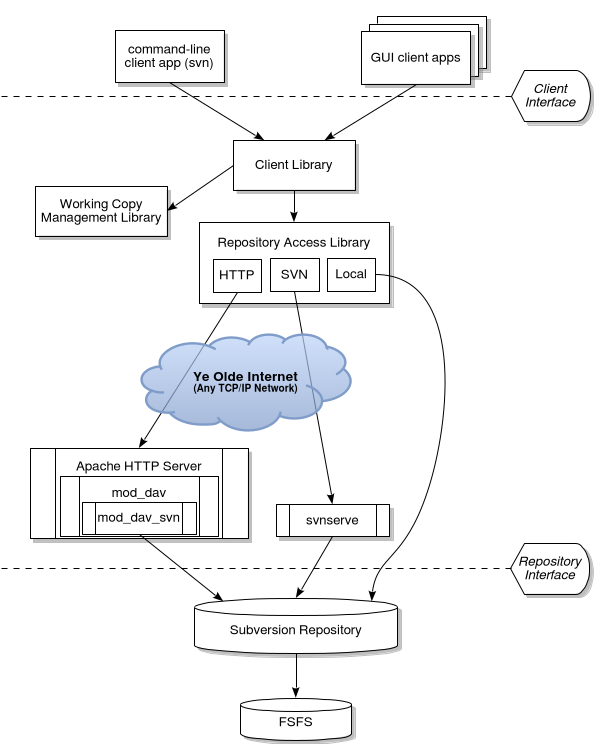
\includegraphics[width=5in,height=6.25in]{images/svn-arch-diagram.png}
\caption{Subversion\textquotesingle s
architecture}\label{svn.intro.architecture.dia-1}
\end{figure}

On one end is a Subversion repository that holds all of your versioned
data. On the other end is your Subversion client program, which manages
local reflections of portions of that versioned data. Between these
extremes are multiple routes through a Repository Access (RA) layer,
some of which go across computer networks and through network servers
which then access the repository, others of which bypass the network
altogether and access the repository directly.

\subsection{Subversion\textquotesingle s
Components}\label{svn.intro.components}

Subversion, once installed, has a number of different pieces. The
following is a quick overview of what you get. Don\textquotesingle t be
alarmed if the brief descriptions leave you scratching your
head---\emph{plenty} more pages in this book are devoted to alleviating
that confusion.

\begin{description}
\item[svn]
The command-line client program
\item[svnversion]
A program for reporting the state (in terms of revisions of the items
present) of a working copy
\item[svnlook]
A tool for directly inspecting a Subversion repository
\item[svnadmin]
A tool for creating, tweaking, or repairing a Subversion repository
\item[mod\_dav\_svn]
A plug-in module for the Apache HTTP Server, used to make your
repository available to others over a network
\item[svnserve]
A custom standalone server program, runnable as a daemon process or
invokable by SSH; another way to make your repository available to
others over a network
\item[svndumpfilter]
A program for filtering Subversion repository dump streams
\item[svnsync]
A program for incrementally mirroring one repository to another over a
network
\item[svnrdump]
A program for performing repository history dumps and loads over a
network
\item[svnmucc]
A program for performing multiple repository URL-based operations in a
single commit and without the use of a working copy
\end{description}

\subsection{What\textquotesingle s New in
Subversion}\label{svn.intro.whatsnew}

The first edition of this book was published by O\textquotesingle Reilly
Media in 2004, shortly after Subversion had reached 1.0. Since that
time, the Subversion project has continued to release new major releases
of the software. Here\textquotesingle s a quick summary of major new
changes since Subversion 1.0. Note that this is not a complete list; for
full details, please visit Subversion\textquotesingle s web site at
\href{https://subversion.apache.org}{}.

\begin{description}
\item[Subversion 1.1 (September 2004)]
Release 1.1 introduced FSFS, a flat-file repository storage option for
the repository. While the Berkeley DB backend is still widely used and
supported, FSFS has since become the default choice for newly created
repositories due to its low barrier to entry and minimal maintenance
requirements. Also in this release came the ability to put symbolic
links under version control, auto-escaping of URLs, and a localized user
interface.
\item[Subversion 1.2 (May 2005)]
Release 1.2 introduced the ability to create server-side locks on files,
thus serializing commit access to certain resources. While Subversion is
still a fundamentally concurrent version control system, certain types
of binary files (e.g. art assets) cannot be merged together. The locking
feature fulfills the need to version and protect such resources. With
locking also came a complete WebDAV auto-versioning implementation,
allowing Subversion repositories to be mounted as network folders.
Finally, Subversion 1.2 began using a new, faster binary-differencing
algorithm to compress and retrieve old versions of files.
\item[Subversion 1.3 (December 2005)]
Release 1.3 brought path-based authorization controls to the
\texttt{svnserve} server, matching a feature formerly found only in the
Apache server. The Apache server, however, gained some new logging
features of its own, and Subversion\textquotesingle s API bindings to
other languages also made great leaps forward.
\item[Subversion 1.4 (September 2006)]
Release 1.4 introduced a whole new tool---\texttt{svnsync}---for doing
one-way repository replication over a network. Major parts of the
working copy metadata were revamped to no longer use XML (resulting in
client-side speed gains), while the Berkeley DB repository backend
gained the ability to automatically recover itself after a server crash.
\item[Subversion 1.5 (June 2008)]
Release 1.5 took much longer to finish than prior releases, but the
headliner feature was gigantic: semi-automated tracking of branching and
merging. This was a huge boon for users, and pushed Subversion far
beyond the abilities of CVS and into the ranks of commercial competitors
such as Perforce and ClearCase. Subversion 1.5 also introduced a bevy of
other user-focused features, such as interactive resolution of file
conflicts, sparse checkouts, client-side management of changelists,
powerful new syntax for externals definitions, and SASL authentication
support for the \texttt{svnserve} server.
\item[Subversion 1.6 (March 2009)]
Release 1.6 continued to make branching and merging more robust by
introducing tree conflicts, and offered improvements to several other
existing features: more interactive conflict resolution options;
de-telescoping and outright exclusion support for sparse checkouts;
file-based externals definitions; and operational logging support for
\texttt{svnserve} similar to what \texttt{mod\_dav\_svn} offered. Also,
the command-line client introduced a new shortcut syntax for referring
to Subversion repository URLs.
\item[Subversion 1.7 (October 2011)]
Release 1.7 was primarily a delivery vehicle for two big plumbing
overhauls of existing Subversion components. The largest and most
impactful of these was the so-called ``WC-NG''---a complete rewrite of
the \texttt{libsvn\_wc} working copy management library. The second
change was the introduction of a sleeker HTTP protocol for Subversion
client/server interaction. Subversion 1.7 delivered a handful of
additional features, many bug fixes, and some notable performance
improvements, too.
\item[Subversion 1.8 (June 2013)]
In release 1.8, Subversion\textquotesingle s client now tracks renamed
files and directories more thoroughly, and its \texttt{svn\ merge}
command has grown intelligent enough to make the
\texttt{-\/-reintegrate} option unnecessary. Certain new versioned
property values can be inherited from parent directories. That feature
now allows a repository to dictate default values for automatic property
settings and ignorable file patterns, bringing consistency across the
user base of that repository in a way which previously had to be managed
socially. There is also a new built-in command-line file merge tool for
interactive conflict resolution. As always, Subversion 1.8 includes many
additional features, defect fixes, and improvements in behavior and
performance.
\end{description}

\section{Audience}\label{svn.preface.audience}

This book is written for computer-literate folk who want to use
Subversion to manage their data. While Subversion runs on a number of
different operating systems, its primary user interface is
command-line-based. That command-line tool (\texttt{svn}), and some
additional auxiliary programs, are the focus of this book.

For consistency, the examples in this book assume that the reader is
using a Unix-like operating system and is relatively comfortable with
Unix and command-line interfaces. That said, the \texttt{svn} program
also runs on non-Unix platforms such as Microsoft Windows. With a few
minor exceptions, such as the use of backward slashes
(\texttt{\textbackslash{}}) instead of forward slashes (\texttt{/}) for
path separators, the input to and output from this tool when run on
Windows are identical to those of its Unix counterpart.

Most readers are probably programmers or system administrators who need
to track changes to source code. This is the most common use for
Subversion, and therefore it is the scenario underlying all of the
book\textquotesingle s examples. But Subversion can be used to manage
changes to any sort of information---images, music, databases,
documentation, and so on. To Subversion, all data is just data.

While this book is written with the assumption that the reader has never
used a version control system, we\textquotesingle ve also tried to make
it easy for users of CVS (and other systems) to make a painless leap
into Subversion. Special sidebars may mention other version control
systems from time to time, and \hyperref[svn.forcvs]{Subversion for CVS
Users} summarizes many of the differences between CVS and Subversion.

Note also that the source code examples used throughout the book are
only examples. While they will compile with the proper compiler
incantations, they are intended to illustrate a particular scenario and
not necessarily to serve as examples of good programming style or
practices.

\section{How to Read This Book}\label{svn.preface.howread}

Technical books always face a certain dilemma: whether to cater to
``top-down'' or to ``bottom-up'' learners. A top-down learner prefers to
read or skim documentation, getting a large overview of how the system
works; only then does she actually start using the software. A bottom-up
learner is a ``learn by doing'' person---someone who just wants to dive
into the software and figure it out as she goes, referring to book
sections when necessary. Most books tend to be written for one type of
person or the other, and this book is undoubtedly biased toward top-down
learners. (And if you\textquotesingle re actually reading this section,
you\textquotesingle re probably already a top-down learner yourself!)
However, if you\textquotesingle re a bottom-up person,
don\textquotesingle t despair. While the book may be laid out as a broad
survey of Subversion topics, the content of each section tends to be
heavy with specific examples that you can try-by-doing. For the
impatient folks who just want to get going, you can jump right to
\hyperref[svn.intro]{Subversion Quick-Start Guide}.

Regardless of your learning style, this book aims to be useful to people
of widely different backgrounds---from those with no previous experience
in version control to experienced system administrators. Depending on
your own background, certain chapters may be more or less important to
you. The following can be considered a ``recommended reading list'' for
various types of readers:

\begin{description}
\item[Experienced system administrators]
The assumption here is that you\textquotesingle ve probably used version
control before and are dying to get a Subversion server up and running
ASAP. \hyperref[svn.reposadmin]{Repository Administration} and
\hyperref[svn.serverconfig]{Server Configuration} will show you how to
create your first repository and make it available over the network.
After that\textquotesingle s done, \hyperref[svn.tour]{Basic Usage} and
\hyperref[svn.forcvs]{Subversion for CVS Users} are the fastest routes
to learning the Subversion client.
\item[New users]
Your administrator has probably set up Subversion already, and you need
to learn how to use the client. If you\textquotesingle ve never used a
version control system, then \hyperref[svn.basic]{Fundamental Concepts}
is a vital introduction to the ideas behind version control.
\hyperref[svn.tour]{Basic Usage} is a guided tour of the Subversion
client.
\item[Advanced users]
Whether you\textquotesingle re a user or administrator, eventually your
project will grow larger. You\textquotesingle re going to want to learn
how to do more advanced things with Subversion, such as how to use
Subversion\textquotesingle s property support
(\hyperref[svn.advanced]{Advanced Topics}), how to use branches and
perform merges (\hyperref[svn.branchmerge]{Branching and Merging}), how
to configure runtime options (\hyperref[svn.customization]{Customizing
Your Subversion Experience}), and other things. These chapters
aren\textquotesingle t critical at first, but be sure to read them once
you\textquotesingle re comfortable with the basics.
\item[Developers]
Presumably, you\textquotesingle re already familiar with Subversion, and
now want to either extend it or build new software on top of its many
APIs. \hyperref[svn.developer]{Embedding Subversion} is just for you.
\end{description}

The book ends with reference material---\hyperref[svn.ref]{Subversion
Command Reference} is a reference guide for all Subversion commands, and
the appendixes cover a number of useful topics. These are the chapters
you\textquotesingle re most likely to come back to after
you\textquotesingle ve finished the book.

\section{Organization of This Book}\label{svn.preface.organization}

The chapters that follow and their contents are listed here:

\begin{description}
\item[{\hyperref[svn.basic]{Fundamental Concepts}}]
Explains the basics of version control and different versioning models,
along with Subversion\textquotesingle s repository, working copies, and
revisions.
\item[{\hyperref[svn.tour]{Basic Usage}}]
Walks you through a day in the life of a Subversion user. It
demonstrates how to use a Subversion client to obtain, modify, and
commit data.
\item[{\hyperref[svn.advanced]{Advanced Topics}}]
Covers more complex features that regular users will eventually come
into contact with, such as versioned metadata, file locking, and peg
revisions.
\item[{\hyperref[svn.branchmerge]{Branching and Merging}}]
Discusses branches, merges, and tagging, including best practices for
branching and merging, common use cases, how to undo changes, and how to
easily swing from one branch to the next.
\item[{\hyperref[svn.reposadmin]{Repository Administration}}]
Describes the basics of the Subversion repository, how to create,
configure, and maintain a repository, and the tools you can use to do
all of this.
\item[{\hyperref[svn.serverconfig]{Server Configuration}}]
Explains how to configure your Subversion server and offers different
ways to access your repository: \texttt{HTTP}, the \texttt{svn}
protocol, and local disk access. It also covers the details of
authentication, authorization and anonymous access.
\item[{\hyperref[svn.customization]{Customizing Your Subversion
Experience}}]
Explores the Subversion client configuration files, the handling of
internationalized text, and how to make external tools cooperate with
Subversion.
\item[{\hyperref[svn.developer]{Embedding Subversion}}]
Describes the internals of Subversion, the Subversion filesystem, and
the working copy administrative areas from a
programmer\textquotesingle s point of view. It also demonstrates how to
use the public APIs to write a program that uses Subversion.
\item[{\hyperref[svn.ref]{Subversion Command Reference}}]
Explains in great detail every subcommand of \texttt{svn},
\texttt{svnadmin}, and \texttt{svnlook} with plenty of examples for the
whole family!
\item[{\hyperref[svn.intro]{Subversion Quick-Start Guide}}]
For the impatient, a whirlwind explanation of how to install Subversion
and start using it immediately. You have been warned.
\item[{\hyperref[svn.forcvs]{Subversion for CVS Users}}]
Covers the similarities and differences between Subversion and CVS, with
numerous suggestions on how to break all the bad habits you picked up
from years of using CVS. Included are descriptions of Subversion
revision numbers, versioned directories, offline operations,
\texttt{update} versus \texttt{status}, branches, tags, metadata,
conflict resolution, and authentication.
\item[{\hyperref[svn.webdav]{WebDAV and Autoversioning}}]
Describes the details of WebDAV and DeltaV and how you can configure
your Subversion repository to be mounted read/write as a DAV share.
\item[{\hyperref[svn.copyright]{Copyright}}]
A copy of the Creative Commons Attribution License, under which this
book is licensed.
\end{description}

\section{This Book Is Free}\label{svn.preface.free}

This book started out as bits of documentation written by Subversion
project developers, which were then coalesced into a single work and
rewritten. As such, it has always been under a free license (see
\hyperref[svn.copyright]{Copyright}). In fact, the book was written in
the public eye, originally as part of the Subversion project itself.
This means two things:

\begin{itemize}
\item
  You will always find the latest version of this book in the
  book\textquotesingle s own Subversion repository.
\item
  You can make changes to this book and redistribute it however you
  wish---it\textquotesingle s under a free license. Your only obligation
  is to maintain proper attribution to the original authors. Of course,
  we\textquotesingle d much rather you send feedback and patches to the
  Subversion developer community, instead of distributing your private
  version of this book.
\end{itemize}

The online home of this book\textquotesingle s development and most of
the volunteer-driven translation efforts regarding it is
\href{https://svnbook.red-bean.com}{}. There you can find links to the
latest releases and tagged versions of the book in various formats, as
well as instructions for accessing the book\textquotesingle s Subversion
repository (where its DocBook XML source code lives). Feedback is
welcomed---encouraged, even. Please submit all comments, complaints, and
patches against the book sources to
\href{mailto:svnbook-dev@red-bean.com}{\nolinkurl{svnbook-dev@red-bean.com}}.

\section{Acknowledgments}\label{svn.preface.acks}

This book would not be possible (nor very useful) if Subversion did not
exist. For that, the authors would like to thank Brian Behlendorf and
CollabNet for the vision to fund such a risky and ambitious new open
source project; Jim Blandy for the original Subversion name and
design---we love you, Jim; and Karl Fogel for being such a good friend
and a great community leader, in that order.\footnote{Oh, and thanks,
  Karl, for being too overworked to write this book yourself.}

Thanks to O\textquotesingle Reilly and the team of professional editors
who have helped us polish this text at various stages of its evolution:
Chuck Toporek, Linda Mui, Tatiana Apandi, Mary Brady, and Mary Treseler.
Your patience and support has been tremendous.

Finally, we thank the countless people who contributed to this book with
informal reviews, suggestions, and patches. An exhaustive listing of
those folks\textquotesingle{} names would be impractical to print and
maintain here, but may their names live on forever in this
book\textquotesingle s version control history!


\part{Getting to Know Subversion}\label{svn.content}

\chapter{Fundamental Concepts}\label{svn.basic}

This chapter is a short, casual introduction to Subversion and its
approach to version control. We begin with a discussion of general
version control concepts, work our way into the specific ideas behind
Subversion, and show some simple examples of Subversion in use.

Even though the examples in this chapter show people sharing collections
of program source code, keep in mind that Subversion can manage any sort
of file collection---it\textquotesingle s not limited to helping
computer programmers.

\section{Version Control Basics}\label{svn.basic.version-control-basics}

A version control system (or revision control system) is a system that
tracks incremental versions (or revisions) of files and, in some cases,
directories over time. Of course, merely tracking the various versions
of a user\textquotesingle s (or group of users\textquotesingle) files
and directories isn\textquotesingle t very interesting in itself. What
makes a version control system useful is the fact that it allows you to
explore the changes which resulted in each of those versions and
facilitates the arbitrary recall of the same.

In this section, we\textquotesingle ll introduce some fairly high-level
version control system components and concepts. We\textquotesingle ll
limit our discussion to modern version control systems---in
today\textquotesingle s interconnected world, there is very little point
in acknowledging version control systems which cannot operate across
wide-area networks.

\subsection{The Repository}\label{svn.basic.repository}

At the core of the version control system is a repository, which is the
central store of that system\textquotesingle s data. The repository
usually stores information in the form of a filesystem tree---a
hierarchy of files and directories. Any number of clients connect to the
repository, and then read or write to these files. By writing data, a
client makes the information available to others; by reading data, the
client receives information from others.
\hyperref[svn.basic.repository.dia-1]{A typical client/server system}
illustrates this.

\begin{figure}
\centering
\pandocbounded{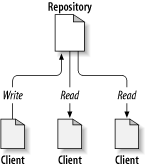
\includegraphics[keepaspectratio]{images/ch02dia1.png}}
\caption{A typical client/server
system}\label{svn.basic.repository.dia-1}
\end{figure}

Why is this interesting? So far, this sounds like the definition of a
typical file server. And indeed, the repository \emph{is} a kind of file
server, but it\textquotesingle s not your usual breed. What makes the
repository special is that as the files in the repository are changed,
the repository remembers each version of those files.

When a client reads data from the repository, it normally sees only the
latest version of the filesystem tree. But what makes a version control
client interesting is that it also has the ability to request previous
states of the filesystem from the repository. A version control client
can ask historical questions such as ``What did this directory contain
last Wednesday?'' and ``Who was the last person to change this file, and
what changes did he make?'' These are the sorts of questions that are at
the heart of any version control system.

\subsection{The Working Copy}\label{svn.basic.working-copy}

A version control system\textquotesingle s value comes from the fact
that it tracks versions of files and directories, but the rest of the
software universe doesn\textquotesingle t operate on ``versions of files
and directories''. Most software programs understand how to operate only
on a \emph{single} version of a specific type of file. So how does a
version control user interact with an abstract---and, often,
remote---repository full of multiple versions of various files in a
concrete fashion? How does his or her word processing software,
presentation software, source code editor, web design software, or some
other program---all of which trade in the currency of simple data
files---get access to such files? The answer is found in the version
control construct known as a working copy.

A working copy is, quite literally, a local copy of a particular version
of a user\textquotesingle s VCS-managed data upon which that user is
free to work. Working copies\footnote{The term ``working copy'' can be
  generally applied to any one file version\textquotesingle s local
  instance. When most folks use the term, though, they are referring to
  a whole directory tree containing files and subdirectories managed by
  the version control system.} appear to other software just as any
other local directory full of files, so those programs
don\textquotesingle t have to be ``version-control-aware'' in order to
read from and write to that data. The task of managing the working copy
and communicating changes made to its contents to and from the
repository falls squarely to the version control
system\textquotesingle s client software.

\subsection{Versioning Models}\label{svn.basic.vsn-models}

If the primary mission of a version control system is to track the
various versions of digital information over time, a very close
secondary mission in any modern version control system is to enable
collaborative editing and sharing of that data. But different systems
use different strategies to achieve this. It\textquotesingle s important
to understand these different strategies, for a couple of reasons.
First, it will help you compare and contrast existing version control
systems, in case you encounter other systems similar to Subversion.
Beyond that, it will also help you make more effective use of
Subversion, since Subversion itself supports a couple of different ways
of working.

\subsubsection{The problem of file
sharing}\label{svn.basic.vsn-models.problem-sharing}

All version control systems have to solve the same fundamental problem:
how will the system allow users to share information, but prevent them
from accidentally stepping on each other\textquotesingle s feet?
It\textquotesingle s all too easy for users to accidentally overwrite
each other\textquotesingle s changes in the repository.

Consider the scenario shown in
\hyperref[svn.basic.vsn-models.problem-sharing.dia-1]{The problem to
avoid}. Suppose we have two coworkers, Harry and Sally. They each decide
to edit the same repository file at the same time. If Harry saves his
changes to the repository first, it\textquotesingle s possible that (a
few moments later) Sally could accidentally overwrite them with her own
new version of the file. While Harry\textquotesingle s version of the
file won\textquotesingle t be lost forever (because the system remembers
every change), any changes Harry made \emph{won\textquotesingle t} be
present in Sally\textquotesingle s newer version of the file, because
she never saw Harry\textquotesingle s changes to begin with.
Harry\textquotesingle s work is still effectively lost---or at least
missing from the latest version of the file---and probably by accident.
This is definitely a situation we want to avoid!

\begin{figure}
\centering
\pandocbounded{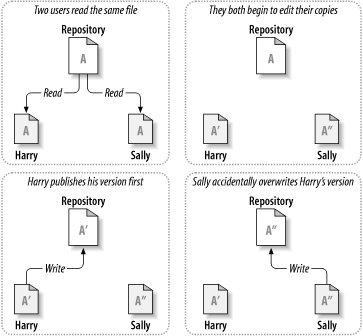
\includegraphics[keepaspectratio]{images/ch02dia2.png}}
\caption{The problem to
avoid}\label{svn.basic.vsn-models.problem-sharing.dia-1}
\end{figure}

\subsubsection{The lock-modify-unlock
solution}\label{svn.basic.vsn-models.lock-unlock}

Many version control systems use a lock-modify-unlock model to address
the problem of many authors clobbering each other\textquotesingle s
work. In this model, the repository allows only one person to change a
file at a time. This exclusivity policy is managed using locks. Harry
must ``lock'' a file before he can begin making changes to it. If Harry
has locked a file, Sally cannot also lock it, and therefore cannot make
any changes to that file. All she can do is wait for Harry to finish his
changes, save the file and release his lock. After Harry unlocks the
file, Sally can take her turn by locking the file. Then she may read the
latest version of the file and edit it.
\hyperref[svn.basic.vsn-models.lock-unlock.dia-1]{The lock-modify-unlock
solution} demonstrates this simple solution.

\begin{figure}
\centering
\pandocbounded{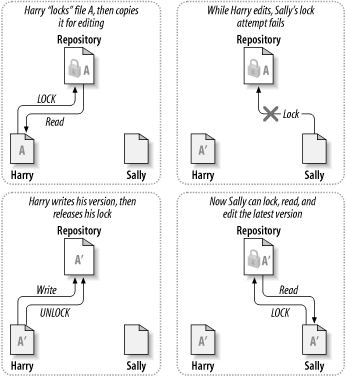
\includegraphics[keepaspectratio]{images/ch02dia3.png}}
\caption{The lock-modify-unlock
solution}\label{svn.basic.vsn-models.lock-unlock.dia-1}
\end{figure}

The problem with the lock-modify-unlock model is that
it\textquotesingle s a bit restrictive and often becomes a roadblock for
users:

\begin{itemize}
\item
  \emph{Locking may cause administrative problems.} Sometimes Harry will
  lock a file and then forget about it. Meanwhile, because Sally is
  still waiting to edit the file, her hands are tied. And then Harry
  goes on vacation. Now Sally has to get an administrator to release
  Harry\textquotesingle s lock. The situation ends up causing a lot of
  unnecessary delay and wasted time.
\item
  \emph{Locking may cause unnecessary serialization.} What if Harry is
  editing the beginning of a text file, and Sally simply wants to edit
  the end of the same file? These changes don\textquotesingle t overlap
  at all. They could easily edit the file simultaneously, and no great
  harm would come, assuming the changes were properly merged together.
  There\textquotesingle s no need for them to take turns in this
  situation.
\item
  \emph{Locking may create a false sense of security.} Suppose Harry
  locks and edits file A, while Sally simultaneously locks and edits
  file B. But what if A and B depend on one another, and the changes
  made to each are semantically incompatible? Suddenly A and B
  don\textquotesingle t work together anymore. The locking system was
  powerless to prevent the problem---yet it somehow provided a false
  sense of security. It\textquotesingle s easy for Harry and Sally to
  imagine that by locking files, each is beginning a safe, insulated
  task, and thus they need not bother discussing their incompatible
  changes early on. Locking often becomes a substitute for real
  communication.
\end{itemize}

\subsubsection{The copy-modify-merge
solution}\label{svn.basic.vsn-models.copy-merge}

Subversion, CVS, and many other version control systems use a
copy-modify-merge model as an alternative to locking. In this model,
each user\textquotesingle s client contacts the project repository and
creates a personal working copy. Users then work simultaneously and
independently, modifying their private copies. Finally, the private
copies are merged together into a new, final version. The version
control system often assists with the merging, but ultimately, a human
being is responsible for making it happen correctly.

Here\textquotesingle s an example. Say that Harry and Sally each create
working copies of the same project, copied from the repository. They
work concurrently and make changes to the same file A within their
copies. Sally saves her changes to the repository first. When Harry
attempts to save his changes later, the repository informs him that his
file A is out of date. In other words, file A in the repository has
somehow changed since he last copied it. So Harry asks his client to
merge any new changes from the repository into his working copy of file
A. Chances are that Sally\textquotesingle s changes
don\textquotesingle t overlap with his own; once he has both sets of
changes integrated, he saves his working copy back to the repository.
\hyperref[svn.basic.vsn-models.copy-merge.dia-1]{The copy-modify-merge
solution} and \hyperref[svn.basic.vsn-models.copy-merge.dia-2]{The
copy-modify-merge solution (continued)} show this process.

\begin{figure}
\centering
\pandocbounded{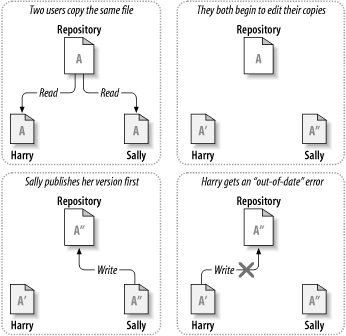
\includegraphics[keepaspectratio]{images/ch02dia4.png}}
\caption{The copy-modify-merge
solution}\label{svn.basic.vsn-models.copy-merge.dia-1}
\end{figure}

\begin{figure}
\centering
\pandocbounded{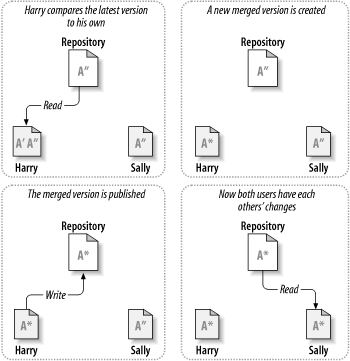
\includegraphics[keepaspectratio]{images/ch02dia5.png}}
\caption{The copy-modify-merge solution
(continued)}\label{svn.basic.vsn-models.copy-merge.dia-2}
\end{figure}

But what if Sally\textquotesingle s changes \emph{do} overlap with
Harry\textquotesingle s changes? What then? This situation is called a
conflict, and it\textquotesingle s usually not much of a problem. When
Harry asks his client to merge the latest repository changes into his
working copy, his copy of file A is somehow flagged as being in a state
of conflict: he\textquotesingle ll be able to see both sets of
conflicting changes and manually choose between them. Note that software
can\textquotesingle t automatically resolve conflicts; only humans are
capable of understanding and making the necessary intelligent choices.
Once Harry has manually resolved the overlapping changes---perhaps after
a discussion with Sally---he can safely save the merged file back to the
repository.

The copy-modify-merge model may sound a bit chaotic, but in practice, it
runs extremely smoothly. Users can work in parallel, never waiting for
one another. When they work on the same files, it turns out that most of
their concurrent changes don\textquotesingle t overlap at all; conflicts
are infrequent. And the amount of time it takes to resolve conflicts is
usually far less than the time lost by a locking system.

In the end, it all comes down to one critical factor: user
communication. When users communicate poorly, both syntactic and
semantic conflicts increase. No system can force users to communicate
perfectly, and no system can detect semantic conflicts. So
there\textquotesingle s no point in being lulled into a false sense of
security that a locking system will somehow prevent conflicts; in
practice, locking seems to inhibit productivity more than anything else.

\protect\phantomsection\label{svn.basic.vsn-models.copy-merge.sb-1}
When Locking Is Necessary

While the lock-modify-unlock model is considered generally harmful to
collaboration, sometimes locking is appropriate.

The copy-modify-merge model is based on the assumption that files are
contextually mergeable---that is, that the majority of the files in the
repository are line-based text files (such as program source code). But
for files with binary formats, such as artwork or sound,
it\textquotesingle s often impossible to merge conflicting changes. In
these situations, it really is necessary for users to take strict turns
when changing the file. Without serialized access, somebody ends up
wasting time on changes that are ultimately discarded.

While Subversion is primarily a copy-modify-merge system, it still
recognizes the need to lock an occasional file, and thus provides
mechanisms for this. We discuss this feature in
\hyperref[svn.advanced.locking]{Locking}.

\section{Version Control the Subversion Way}\label{svn.basic.in-action}

We\textquotesingle ve mentioned already that Subversion is a modern,
network-aware version control system. As we described in
\hyperref[svn.basic.version-control-basics]{Version Control Basics} (our
high-level version control overview), a repository serves as the core
storage mechanism for Subversion\textquotesingle s versioned data, and
it\textquotesingle s via working copies that users and their software
programs interact with that data. In this section, we\textquotesingle ll
begin to introduce the specific ways in which Subversion implements
version control.

\subsection{Subversion Repositories}\label{svn.basic.svn-repositories}

Subversion implements the concept of a version control repository much
as any other modern version control system would. Unlike a working copy,
a Subversion repository is an abstract entity, able to be operated upon
almost exclusively by Subversion\textquotesingle s own libraries and
tools. As most of a user\textquotesingle s Subversion interactions
involve the use of the Subversion client and occur in the context of a
working copy, we spend the majority of this book discussing the
Subversion working copy and how to manipulate it. For the finer details
of the repository, though, check out
\hyperref[svn.reposadmin]{Repository Administration}.

\protect\phantomsection\label{svn.basic.svn-repositories.not-working-copy}
In Subversion, the client-side object which every user of the system
has---the directory of versioned files, along with metadata that enables
the system to track them and communicate with the server---is called a
\emph{working copy}. Although other version control systems use the term
``repository'' for the client-side object, it is both incorrect and a
common source of confusion to use the term in that way in the context of
Subversion.

Working copies are described later, in
\hyperref[svn.basic.in-action.wc]{Subversion Working Copies}.

\subsection{Revisions}\label{svn.basic.in-action.revs}

A Subversion client commits (that is, communicates the changes made to)
any number of files and directories as a single atomic transaction. By
atomic transaction, we mean simply this: either all of the changes are
accepted into the repository, or none of them is. Subversion tries to
retain this atomicity in the face of program crashes, system crashes,
network problems, and other users\textquotesingle{} actions.

Each time the repository accepts a commit, this creates a new state of
the filesystem tree, called a revision. Each revision is assigned a
unique natural number, one greater than the number assigned to the
previous revision. The initial revision of a freshly created repository
is numbered 0 and consists of nothing but an empty root directory.

\hyperref[svn.basic.in-action.revs.dia-1]{Tree changes over time}
illustrates a nice way to visualize the repository. Imagine an array of
revision numbers, starting at 0, stretching from left to right. Each
revision number has a filesystem tree hanging below it, and each tree is
a ``snapshot'' of the way the repository looked after a commit.

\begin{figure}
\centering
\pandocbounded{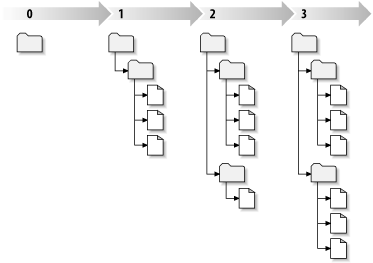
\includegraphics[keepaspectratio]{images/ch02dia7.png}}
\caption{Tree changes over time}\label{svn.basic.in-action.revs.dia-1}
\end{figure}

Global Revision Numbers

Unlike most version control systems, Subversion\textquotesingle s
revision numbers apply to \emph{the entire repository tree}, not
individual files. Each revision number selects an entire tree, a
particular state of the repository after some committed change. Another
way to think about it is that revision N represents the state of the
repository filesystem after the Nth commit. When Subversion users talk
about ``revision 5 of \texttt{foo.c},'' they really mean
``\texttt{foo.c} as it appears in revision 5.'' Notice that in general,
revisions N and M of a file do \emph{not} necessarily differ! Many other
version control systems use per-file revision numbers, so this concept
may seem unusual at first. (Former CVS users might want to see
\hyperref[svn.forcvs]{Subversion for CVS Users} for more details.)

\subsection{Addressing the Repository}\label{svn.advanced.reposurls}

Subversion client programs use URLs to identify versioned files and
directories in Subversion repositories. For the most part, these URLs
use the standard syntax, allowing for server names and port numbers to
be specified as part of the URL.

\begin{itemize}
\tightlist
\item
  http://svn.example.com/svn/project
\item
  http://svn.example.com:9834/repos
\end{itemize}

Subversion repository URLs aren\textquotesingle t limited to only the
\texttt{http://} variety. Because Subversion offers several different
ways for its clients to communicate with its servers, the URLs used to
address the repository differ subtly depending on which repository
access mechanism is employed.
\hyperref[svn.basic.in-action.wc.tbl-1]{Repository access URLs}
describes how different URL schemes map to the available repository
access methods. For more details about Subversion\textquotesingle s
server options, see \hyperref[svn.serverconfig]{Server Configuration}.

\begin{longtable}[]{@{}>{\raggedright\arraybackslash}p{\dimexpr(\linewidth-2\tabcolsep*2)/2\relax}>{\raggedright\arraybackslash}p{\dimexpr(\linewidth-2\tabcolsep*2)/2\relax}@{}}
\caption{Repository access
URLs}\label{svn.basic.in-action.wc.tbl-1}\tabularnewline
\toprule\noalign{}
Schema & Access method \\
\midrule\noalign{}
\endfirsthead
\toprule\noalign{}
Schema & Access method \\
\midrule\noalign{}
\endhead
\bottomrule\noalign{}
\endlastfoot
\texttt{file:///} & Direct repository access (on local disk) \\
\texttt{http://} & Access via WebDAV protocol to Subversion-aware Apache
server \\
\texttt{https://} & Same as \texttt{http://}, but with SSL encapsulation
(encryption and authentication) \\
\texttt{svn://} & Access via custom protocol to an \texttt{svnserve}
server \\
\texttt{svn+ssh://} & Same as \texttt{svn://}, but through an SSH
tunnel \\
\end{longtable}

Subversion\textquotesingle s handling of URLs has some noteworthy
nuances. For example, URLs containing the \texttt{file://} access method
(used for local repositories) must, in accordance with convention, have
either a server name of \texttt{localhost} or no server name at all:

\begin{itemize}
\tightlist
\item
  file:///var/svn/repos
\item
  file://localhost/var/svn/repos
\end{itemize}

Also, users of the \texttt{file://} scheme on Windows platforms will
need to use an unofficially ``standard'' syntax for accessing
repositories that are on the same machine, but on a different drive than
the client\textquotesingle s current working drive. Either of the two
following URL path syntaxes will work, where \texttt{X} is the drive on
which the repository resides:

\begin{itemize}
\tightlist
\item
  file:///X:/var/svn/repos
\item
  file:///X\textbar/var/svn/repos
\end{itemize}

Note that a URL uses forward slashes even though the native (non-URL)
form of a path on Windows uses backslashes. Also note that when using
the \texttt{file:///X\textbar{}/} form at the command line, you need to
quote the URL (wrap it in quotation marks) so that the vertical bar
character is not interpreted as a pipe.

You cannot use Subversion\textquotesingle s \texttt{file://} URLs in a
regular web browser the way you can use typical \texttt{file://} URLs.
When you attempt to view a \texttt{file://} URL in a regular web
browser, it reads and displays the contents of the file at that location
by examining the filesystem directly. However,
Subversion\textquotesingle s resources exist in a virtual filesystem
(see \hyperref[svn.developer.layerlib.repos]{Repository Layer}), and
your browser will not understand how to interact with that filesystem.

The Subversion client will automatically encode URLs as necessary, just
like a web browser does. For example, the URL
\texttt{http://host/path\ with\ space/project/españa} --- which contains
both spaces and upper-ASCII characters --- will be automatically
interpreted by Subversion as if you\textquotesingle d provided
\texttt{http://host/path\%20with\%20space/project/espa\%C3\%B1a}. If the
URL contains spaces, be sure to place it within quotation marks at the
command line so that your shell treats the whole thing as a single
argument to the program.

There is one notable exception to Subversion\textquotesingle s handling
of URLs which also applies to its handling of local paths in many
contexts, too. If the final path component of your URL or local path
contains an at sign (\texttt{@}), you need to use a special
syntax---described in \hyperref[svn.advanced.pegrevs]{Peg and Operative
Revisions}---in order to make Subversion properly address that resource.

In Subversion 1.6, a new caret (\texttt{\^{}}) notation was introduced
as a shorthand for ``the URL of the repository\textquotesingle s root
directory''. For example, you can use the
\texttt{\^{}/tags/bigsandwich/} to refer to the URL of the
\texttt{/tags/bigsandwich} directory in the root of the repository. Such
a URL is called a repository-relative URL. Note that this URL syntax
works only when your current working directory is a working copy---the
command-line client knows the repository\textquotesingle s root URL by
looking at the working copy\textquotesingle s metadata. Also note that
when you wish to refer precisely to the root directory of the
repository, you must do so using \texttt{\^{}/} (with the trailing slash
character), not merely \texttt{\^{}}. Windows users should not forget
that a caret is an escape character on their platform. Therefore, use a
double caret \texttt{\^{}\^{}} if you run the Subversion client on a
Windows machine.

\subsection{Subversion Working Copies}\label{svn.basic.in-action.wc}

A Subversion working copy is an ordinary directory tree on your local
system, containing a collection of files. You can edit these files
however you wish, and if they\textquotesingle re source code files, you
can compile your program from them in the usual way. Your working copy
is your own private work area: Subversion will never incorporate other
people\textquotesingle s changes, nor make your own changes available to
others, until you explicitly tell it to do so. You can even have
multiple working copies of the same project.

After you\textquotesingle ve made some changes to the files in your
working copy and verified that they work properly, Subversion provides
you with commands to ``publish'' your changes (by writing to the
repository), thereby making them available to the other people working
with you on your project. If other people publish their own changes,
Subversion provides you with commands to merge those changes into your
own working copy (by reading from the repository). Notice that the
central repository is the broker for everybody\textquotesingle s changes
in Subversion---changes aren\textquotesingle t passed directly from
working copy to working copy in the typical workflow.

A working copy also contains some extra files, created and maintained by
Subversion, to help it carry out these commands. In particular, each
working copy contains a subdirectory named \texttt{.svn}, also known as
the working copy\textquotesingle s administrative directory. The files
in the administrative directory help Subversion recognize which of your
versioned files contain unpublished changes, and which files are out of
date with respect to others\textquotesingle{} work.

Prior to version 1.7, Subversion maintained \texttt{.svn} administrative
subdirectories in \emph{every} versioned directory of your working copy.
Subversion 1.7 offers a completely new approach to how working copy
metadata is stored and maintained, and chief among the visible changes
to this approach is that each working copy now has only one
\texttt{.svn} subdirectory which is an immediate child of the root of
that working copy.

\subsubsection{How the working copy
works}\label{svn.basic.in-action.track-repos}

For each file in a working directory, Subversion records (among other
things) two essential pieces of information:

\begin{itemize}
\item
  What revision your working file is based on (this is called the
  file\textquotesingle s working revision)
\item
  A timestamp recording when the local copy was last updated by the
  repository
\end{itemize}

Given this information, by talking to the repository, Subversion can
tell which of the following four states a working file is in:

\begin{description}
\item[Unchanged, and current]
The file is unchanged in the working directory, and no changes to that
file have been committed to the repository since its working revision.
An \texttt{svn\ commit} of the file will do nothing, and an
\texttt{svn\ update} of the file will do nothing.
\item[Locally changed, and current]
The file has been changed in the working directory, and no changes to
that file have been committed to the repository since you last updated.
There are local changes that have not been committed to the repository;
thus an \texttt{svn\ commit} of the file will succeed in publishing your
changes, and an \texttt{svn\ update} of the file will do nothing.
\item[Unchanged, and out of date]
The file has not been changed in the working directory, but it has been
changed in the repository. The file should eventually be updated in
order to make it current with the latest public revision. An
\texttt{svn\ commit} of the file will do nothing, and an
\texttt{svn\ update} of the file will fold the latest changes into your
working copy.
\item[Locally changed, and out of date]
The file has been changed both in the working directory and in the
repository. An \texttt{svn\ commit} of the file will fail with an
``out-of-date'' error. The file should be updated first; an
\texttt{svn\ update} command will attempt to merge the public changes
with the local changes. If Subversion can\textquotesingle t complete the
merge in a plausible way automatically, it leaves it to the user to
resolve the conflict.
\end{description}

\subsubsection{Fundamental working copy
interactions}\label{svn.basic.in-action.wc-funcdamentals}

A typical Subversion repository often holds the files (or source code)
for several projects; usually, each project is a subdirectory in the
repository\textquotesingle s filesystem tree. In this arrangement, a
user\textquotesingle s working copy will usually correspond to a
particular subtree of the repository.

For example, suppose you have a repository that contains two software
projects, \texttt{paint} and \texttt{calc}. Each project lives in its
own top-level subdirectory, as shown in
\hyperref[svn.basic.in-action.wc.dia-1]{The repository\textquotesingle s
filesystem}.

\begin{figure}
\centering
\pandocbounded{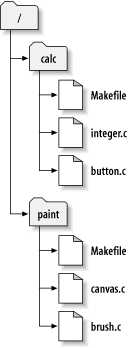
\includegraphics[keepaspectratio]{images/ch02dia6.png}}
\caption{The repository\textquotesingle s
filesystem}\label{svn.basic.in-action.wc.dia-1}
\end{figure}

To get a working copy, you must check out some subtree of the
repository. (The term \emph{check out} may sound like it has something
to do with locking or reserving resources, but it
doesn\textquotesingle t; it simply creates a working copy of the project
for you.) For example, if you check out \texttt{/calc}, you will get a
working copy like this:

\begin{verbatim}
$ svn checkout http://svn.example.com/repos/calc
A    calc/Makefile
A    calc/integer.c
A    calc/button.c
Checked out revision 56.
$ ls -A calc
Makefile  button.c integer.c .svn/
$
\end{verbatim}

The list of letter \texttt{A}s in the left margin indicates that
Subversion is adding a number of items to your working copy. You now
have a personal copy of the repository\textquotesingle s \texttt{/calc}
directory, with one additional entry---\texttt{.svn}---which holds the
extra information needed by Subversion, as mentioned earlier.

Suppose you make changes to \texttt{button.c}. Since the \texttt{.svn}
directory remembers the file\textquotesingle s original modification
date and contents, Subversion can tell that you\textquotesingle ve
changed the file. However, Subversion does not make your changes public
until you explicitly tell it to. The act of publishing your changes is
more commonly known as committing (or checking in) changes to the
repository.

To publish your changes, you can use Subversion\textquotesingle s
\texttt{svn\ commit} command:

\begin{verbatim}
$ svn commit button.c -m "Fixed a typo in button.c."
Sending        button.c
Transmitting file data .
Committed revision 57.
$
\end{verbatim}

Now your changes to \texttt{button.c} have been committed to the
repository, with a note describing your change (namely, that you fixed a
typo). If another user checks out a working copy of \texttt{/calc}, she
will see your changes in the latest version of the file.

Suppose you have a collaborator, Sally, who checked out a working copy
of \texttt{/calc} at the same time you did. When you commit your change
to \texttt{button.c}, Sally\textquotesingle s working copy is left
unchanged; Subversion modifies working copies only at the
user\textquotesingle s request.

To bring her project up to date, Sally can ask Subversion to update her
working copy, by using the \texttt{svn\ update} command. This will
incorporate your changes into her working copy, as well as any others
that have been committed since she checked it out.

\begin{verbatim}
$ pwd
/home/sally/calc
$ ls -A
Makefile button.c integer.c .svn/
$ svn update
Updating '.':
U    button.c
Updated to revision 57.
$
\end{verbatim}

The output from the \texttt{svn\ update} command indicates that
Subversion updated the contents of \texttt{button.c}. Note that Sally
didn\textquotesingle t need to specify which files to update; Subversion
uses the information in the \texttt{.svn} directory as well as further
information in the repository, to decide which files need to be brought
up to date.

\subsubsection{Mixed-revision working
copies}\label{svn.basic.in-action.mixedrevs}

As a general principle, Subversion tries to be as flexible as possible.
One special kind of flexibility is the ability to have a working copy
containing files and directories with a mix of different working
revision numbers. Subversion working copies do not always correspond to
any single revision in the repository; they may contain files from
several different revisions. For example, suppose you check out a
working copy from a repository whose most recent revision is 4:

\begin{verbatim}
calc/
   Makefile:4
   integer.c:4
   button.c:4
\end{verbatim}

At the moment, this working directory corresponds exactly to revision 4
in the repository. However, suppose you make a change to
\texttt{button.c}, and commit that change. Assuming no other commits
have taken place, your commit will create revision 5 of the repository,
and your working copy will now look like this:

\begin{verbatim}
calc/
   Makefile:4
   integer.c:4
   button.c:5
\end{verbatim}

Suppose that, at this point, Sally commits a change to
\texttt{integer.c}, creating revision 6. If you use \texttt{svn\ update}
to bring your working copy up to date, it will look like this:

\begin{verbatim}
calc/
   Makefile:6
   integer.c:6
   button.c:6
\end{verbatim}

Sally\textquotesingle s change to \texttt{integer.c} will appear in your
working copy, and your change will still be present in
\texttt{button.c}. In this example, the text of \texttt{Makefile} is
identical in revisions 4, 5, and 6, but Subversion will mark your
working copy of \texttt{Makefile} with revision 6 to indicate that it is
still current. So, after you do a clean update at the top of your
working copy, it will generally correspond to exactly one revision in
the repository.

\paragraph{Updates and commits are
separate}\label{svn.basic.in-action.mixedrevs.update-commit}

One of the fundamental rules of Subversion is that a ``push'' action
does not cause a ``pull'' nor vice versa. Just because
you\textquotesingle re ready to submit new changes to the repository
doesn\textquotesingle t mean you\textquotesingle re ready to receive
changes that others have checked in. And if you have new changes still
in progress, \texttt{svn\ update} should gracefully merge repository
changes into your own, rather than forcing you to publish them.

The main side effect of this rule is that it means a working copy has to
do extra bookkeeping to track mixed revisions as well as be tolerant of
the mixture. It\textquotesingle s made more complicated by the fact that
directories themselves are versioned.

For example, suppose you have a working copy entirely at revision 10,
while others have been committing their changes so that the youngest
revision in the repository is now revision 14. You edit the file
\texttt{foo.html} and then perform an \texttt{svn\ commit}, which
creates revision 15 in the repository. After the commit succeeds, many
new users would expect the working copy to be entirely at revision 15,
but that\textquotesingle s not the case! Any number of changes might
have happened in the repository between revisions 10 and 15. The client
knows nothing of those changes in the repository, since you
haven\textquotesingle t yet run \texttt{svn\ update}, and
\texttt{svn\ commit} doesn\textquotesingle t pull down new changes. If,
on the other hand, \texttt{svn\ commit} were to automatically download
the newest changes, it would be possible to set the entire working copy
to revision 15---but then we\textquotesingle d be breaking the
fundamental rule of ``push'' and ``pull'' remaining separate actions.
Therefore, the only safe thing the Subversion client can do is mark the
one file---\texttt{foo.html}---as being at revision 15. The rest of the
working copy remains at revision 10. Only by running
\texttt{svn\ update} can the latest changes be downloaded and the whole
working copy be marked as revision 15.

\paragraph{Mixed revisions are
normal}\label{svn.basic.in-action.mixedrevs.normal}

The fact is, \emph{every time} you run \texttt{svn\ commit} your working
copy ends up with some mixture of revisions. The things you just
committed are marked as having larger working revisions than everything
else. After several commits (with no updates in between), your working
copy will contain a whole mixture of revisions. Even if
you\textquotesingle re the only person using the repository, you will
still see this phenomenon. To examine your mixture of working revisions,
use the \texttt{svn\ status} command with the \texttt{-\/-verbose}
(\texttt{-v}) option (see \hyperref[svn.tour.cycle.examine.status]{See
an overview of your changes} for more information).

Often, new users are completely unaware that their working copy contains
mixed revisions. This can be confusing, because many client commands are
sensitive to the working revision of the item they\textquotesingle re
examining. For example, the \texttt{svn\ log} command is used to display
the history of changes to a file or directory (see
\hyperref[svn.tour.history.log]{Generating a List of Historical
Changes}). When the user invokes this command on a working copy object,
he expects to see the entire history of the object. But if the
object\textquotesingle s working revision is quite old (often because
\texttt{svn\ update} hasn\textquotesingle t been run in a long time),
the history of the \emph{older} version of the object is shown.

\paragraph{Mixed revisions are
useful}\label{svn.basic.in-action.mixedrevs.useful}

If your project is sufficiently complex, you\textquotesingle ll discover
that it\textquotesingle s sometimes nice to forcibly backdate (or update
to a revision older than the one you already have) portions of your
working copy to an earlier revision; you\textquotesingle ll learn how to
do that in \hyperref[svn.tour]{Basic Usage}. Perhaps
you\textquotesingle d like to test an earlier version of a submodule
contained in a subdirectory, or perhaps you\textquotesingle d like to
figure out when a bug first came into existence in a specific file. This
is the ``time machine'' aspect of a version control system---the feature
that allows you to move any portion of your working copy forward and
backward in history.

\paragraph{Mixed revisions have
limitations}\label{svn.basic.in-action.mixedrevs.limits}

However you make use of mixed revisions in your working copy, there are
limitations to this flexibility.

First, you cannot commit the deletion of a file or directory that
isn\textquotesingle t fully up to date. If a newer version of the item
exists in the repository, your attempt to delete will be rejected to
prevent you from accidentally destroying changes you\textquotesingle ve
not yet seen.

Second, you cannot commit a metadata change to a directory unless
it\textquotesingle s fully up to date. You\textquotesingle ll learn
about attaching ``properties'' to items in
\hyperref[svn.advanced]{Advanced Topics}. A directory\textquotesingle s
working revision defines a specific set of entries and properties, and
thus committing a property change to an out-of-date directory may
destroy properties you\textquotesingle ve not yet seen.

Finally, beginning in Subversion 1.7, you cannot by default use a
mixed-revision working copy as the target of a merge operation. (This
new requirement was introduced to prevent common problems which stem
from doing so.)

\section{Summary}\label{svn.basic.summary}

We covered a number of fundamental Subversion concepts in this chapter:

\begin{itemize}
\item
  We introduced the notions of the central repository, the client
  working copy, and the array of repository revision trees.
\item
  We saw some simple examples of how two collaborators can use
  Subversion to publish and receive changes from one another, using the
  ``copy-modify-merge'' model.
\item
  We talked a bit about the way Subversion tracks and manages
  information in a working copy.
\end{itemize}

At this point, you should have a good idea of how Subversion works in
the most general sense. Armed with this knowledge, you should now be
ready to move into the next chapter, which is a detailed tour of
Subversion\textquotesingle s commands and features.


\chapter{Basic Usage}\label{svn.tour}

Theory is useful, but its application is just plain fun.
Let\textquotesingle s move now into the details of using Subversion. By
the time you reach the end of this chapter, you will be able to perform
all the tasks you need to use Subversion in a normal
day\textquotesingle s work. You\textquotesingle ll start with getting
your files into Subversion, followed by an initial checkout of your
code. We\textquotesingle ll then walk you through making changes and
examining those changes. You\textquotesingle ll also see how to bring
changes made by others into your working copy, examine them, and work
through any conflicts that might arise.

This chapter will not provide exhaustive coverage of all of
Subversion\textquotesingle s commands---rather, it\textquotesingle s a
conversational introduction to the most common Subversion tasks that
you\textquotesingle ll encounter. This chapter assumes that
you\textquotesingle ve read and understood
\hyperref[svn.basic]{Fundamental Concepts} and are familiar with the
general model of Subversion. For a complete reference of all commands,
see \hyperref[svn.ref.svn]{svn Reference---Subversion Command-Line
Client}.

Also, this chapter assumes that the reader is seeking information about
how to interact in a basic fashion with an existing Subversion
repository. No repository means no working copy; no working copy means
not much of interest in this chapter. There are many Internet sites
which offer free or inexpensive Subversion repository hosting services.
Or, if you\textquotesingle d prefer to set up and administer your own
repositories, check out \hyperref[svn.reposadmin]{Repository
Administration}. But don\textquotesingle t expect the examples in this
chapter to work without the user having access to a Subversion
repository.

Finally, any Subversion operation that contacts the repository over a
network may potentially require that the user authenticate. For the sake
of simplicity, our examples throughout this chapter avoid demonstrating
and discussing authentication. Be aware that if you hope to apply the
knowledge herein to an existing, real-world Subversion instance,
you\textquotesingle ll probably be forced to provide at least a username
and password to the server. See
\hyperref[svn.serverconfig.netmodel.creds]{Client Credentials} for a
detailed description of Subversion\textquotesingle s handling of
authentication and client credentials.

\section{Help!}\label{svn.tour.help}

It goes without saying that this book exists to be a source of
information and assistance for Subversion users new and old.
Conveniently, though, the Subversion command-line is self-documenting,
alleviating the need to grab a book off the shelf (wooden, virtual, or
otherwise). The \texttt{svn\ help} command is your gateway to that
built-in documentation:

\begin{verbatim}
$ svn help
usage: svn <subcommand> [options] [args]
Subversion command-line client, version 1.8.13.
Type 'svn help <subcommand>' for help on a specific subcommand.
Type 'svn --version' to see the program version and RA modules
  or 'svn --version --quiet' to see just the version number.

Most subcommands take file and/or directory arguments, recursing
on the directories.  If no arguments are supplied to such a
command, it recurses on the current directory (inclusive) by default.

Available subcommands:
   add
   blame (praise, annotate, ann)
   cat
…
\end{verbatim}

As described in the previous output, you can ask for help on a
particular subcommand by running \texttt{svn\ help\ SUBCOMMAND}.
Subversion will respond with the full usage message for that subcommand,
including its syntax, options, and behavior:

\begin{verbatim}
$ svn help help
help (?, h): Describe the usage of this program or its subcommands.
usage: help [SUBCOMMAND...]

Global options:
  --username ARG           : specify a username ARG
  --password ARG           : specify a password ARG
…
\end{verbatim}

Options and Switches and Flags, Oh My!

The Subversion command-line client has numerous command modifiers. Some
folks refer to such things as ``switches'' or ``flags''---in this book,
we\textquotesingle ll call them ``options''. You\textquotesingle ll find
the options supported by a given \texttt{svn} subcommand, plus a set of
options which are globally supported by all subcommands, listed near the
bottom of the built-in usage message for that subcommand.

Subversion\textquotesingle s options have two distinct forms: short
options are a single hyphen followed by a single letter, and long
options consist of two hyphens followed by several letters and hyphens
(e.g., \texttt{-s} and \texttt{-\/-this-is-a-long-option},
respectively). Every option has at least one long format. Some, such as
the \texttt{-\/-changelist} option, feature an abbreviated long-format
alias (\texttt{-\/-cl}, in this case). Only certain options---generally
the most-used ones---have an additional short format. To maintain
clarity in this book, we usually use the long form in code examples, but
when describing options, if there\textquotesingle s a short form,
we\textquotesingle ll provide the long form (to improve clarity) and the
short form (to make it easier to remember). Use the form
you\textquotesingle re more comfortable with when executing your own
Subversion commands.

Many Unix-based distributions of Subversion include manual pages of the
sort that can be invoked using the \texttt{man} program, but those tend
to carry only pointers to other sources of real help, such as the
project\textquotesingle s website and to the website which hosts this
book. Also, several companies offer Subversion help and support, too,
usually via a mixture of web-based discussion forums and fee-based
consulting. And of course, the Internet holds a decade\textquotesingle s
worth of Subversion-related discussions just begging to be located by
your favorite search engine. Subversion help is never too far away.

\section{Getting Data into Your Repository}\label{svn.tour.importing}

You can get new files into your Subversion repository in two ways:
\texttt{svn\ import} and \texttt{svn\ add}. We\textquotesingle ll
discuss \texttt{svn\ import} now and will discuss \texttt{svn\ add}
later in this chapter when we review a typical day with Subversion.

\subsection{Importing Files and
Directories}\label{svn.tour.importing.import}

The \texttt{svn\ import} command is a quick way to copy an unversioned
tree of files into a repository, creating intermediate directories as
necessary. \texttt{svn\ import} doesn\textquotesingle t require a
working copy, and your files are immediately committed to the
repository. You typically use this when you have an existing tree of
files that you want to begin tracking in your Subversion repository. For
example:

\begin{verbatim}
$ svn import /path/to/mytree \
             http://svn.example.com/svn/repo/some/project \
             -m "Initial import"
Adding         mytree/foo.c
Adding         mytree/bar.c
Adding         mytree/subdir
Adding         mytree/subdir/quux.h

Committed revision 1.
$
\end{verbatim}

The previous example copied the contents of the local directory
\texttt{mytree} into the directory \texttt{some/project} in the
repository. Note that you didn\textquotesingle t have to create that new
directory first---\texttt{svn\ import} does that for you. Immediately
after the commit, you can see your data in the repository:

\begin{verbatim}
$ svn list http://svn.example.com/svn/repo/some/project
bar.c
foo.c
subdir/
$
\end{verbatim}

Note that after the import is finished, the original local directory is
\emph{not} converted into a working copy. To begin working on that data
in a versioned fashion, you still need to create a fresh working copy of
that tree.

\subsection{Recommended Repository
Layout}\label{svn.tour.importing.layout}

Subversion provides the ultimate flexibility in terms of how you arrange
your data. Because it simply versions directories and files, and because
it ascribes no particular meaning to any of those objects, you may
arrange the data in your repository in any way that you choose.
Unfortunately, this flexibility also means that it\textquotesingle s
easy to find yourself ``lost without a roadmap'' as you attempt to
navigate different Subversion repositories which may carry completely
different and unpredictable arrangements of the data within them.

To counteract this confusion, we recommend that you follow a repository
layout convention (established long ago, in the nascency of the
Subversion project itself) in which a handful of strategically named
Subversion repository directories convey valuable meaning about the data
they hold. Most projects have a recognizable ``main line'', or trunk, of
development; some branches, which are divergent copies of development
lines; and some tags, which are named, stable snapshots of a particular
line of development. So we first recommend that each project have a
recognizable project root in the repository, a directory under which all
of the versioned information for that project---and only that
project---lives. Secondly, we suggest that each project root contain a
\texttt{trunk} subdirectory for the main development line, a
\texttt{branches} subdirectory in which specific branches (or
collections of branches) will be created, and a \texttt{tags}
subdirectory in which specific tags (or collections of tags) will be
created. Of course, if a repository houses only a single project, the
root of the repository can serve as the project root, too.

Here are some examples:

\begin{verbatim}
$ svn list file:///var/svn/single-project-repo
trunk/
branches/
tags/
$ svn list file:///var/svn/multi-project-repo
project-A/
project-B/
$ svn list file:///var/svn/multi-project-repo/project-A
trunk/
branches/
tags/
$
\end{verbatim}

We talk much more about tags and branches in
\hyperref[svn.branchmerge]{Branching and Merging}. For details and some
advice on how to set up repositories when you have multiple projects,
see \hyperref[svn.branchmerge.maint.layout]{Repository Layout}. Finally,
we discuss project roots more in
\hyperref[svn.reposadmin.projects.chooselayout]{Planning Your Repository
Organization}.

\subsection{What\textquotesingle s In a
Name?}\label{svn.tour.importing.naming}

Subversion tries hard not to limit the type of data you can place under
version control. The contents of files and property values are stored
and transmitted as binary data, and
\hyperref[svn.advanced.props.special.mime-type]{File Content Type} tells
you how to give Subversion a hint that ``textual'' operations
don\textquotesingle t make sense for a particular file. There are a few
places, however, where Subversion places restrictions on information it
stores.

Subversion internally handles certain bits of data---for example,
property names, pathnames, and log messages---as UTF-8-encoded Unicode.
This is not to say that all your interactions with Subversion must
involve UTF-8, though. As a general rule, Subversion clients will
gracefully and transparently handle conversions between UTF-8 and the
encoding system in use on your computer, if such a conversion can
meaningfully be done (which is the case for most common encodings in use
today).

In WebDAV exchanges and older versions of some of
Subversion\textquotesingle s administrative files, paths are used as XML
attribute values, and property names in XML tag names. This means that
pathnames can contain only legal XML (1.0) characters, and properties
are further limited to ASCII characters. Subversion also prohibits
\texttt{TAB}, \texttt{CR}, and \texttt{LF} characters in path names to
prevent paths from being broken up in diffs or in the output of commands
such as \texttt{svn\ log} or \texttt{svn\ status}.

While it may seem like a lot to remember, in practice these limitations
are rarely a problem. As long as your locale settings are compatible
with UTF-8 and you don\textquotesingle t use control characters in path
names, you should have no trouble communicating with Subversion. The
command-line client adds an extra bit of help---to create ``legally
correct'' versions for internal use it will automatically escape illegal
path characters as needed in URLs that you type.

Of course, when it comes to choosing valid path names, Subversion
isn\textquotesingle t the only limiting factor. Teams using multiple
operating systems need to consider the limitations placed on path names
by those operating systems, too. For example, while Windows disallows
the use of colon characters in file names, a user on a Linux system can
very easily add such a file to version control, resulting in a dataset
that can no longer be checked out on Windows. Adding multiple files to a
directory whose names differ only in their letter casing will likewise
cause problems for users checking out working copies onto
case-insensitive filesystems. So, some broad awareness of the various
limitations introduced by different operating systems and filesystems,
then, is recommended.

\section{Creating a Working Copy}\label{svn.tour.initial}

Most of the time, you will start using a Subversion repository by
performing a checkout of your project. Checking out a directory from a
repository creates a working copy of that directory on your local
machine. Unless otherwise specified, this copy contains the youngest
(that is, most recently created or modified) versions of the directory
and its children found in the Subversion repository:

\begin{verbatim}
$ svn checkout http://svn.example.com/svn/repo/trunk
A    trunk/README
A    trunk/INSTALL
A    trunk/src/main.c
A    trunk/src/header.h
…
Checked out revision 8810.
$
\end{verbatim}

Although the preceding example checks out the trunk directory, you can
just as easily check out a deeper subdirectory of a repository by
specifying that subdirectory\textquotesingle s URL as the checkout URL:

\begin{verbatim}
$ svn checkout http://svn.example.com/svn/repo/trunk/src
A    src/main.c
A    src/header.h
A    src/lib/helpers.c
…
Checked out revision 8810.
$
\end{verbatim}

Since Subversion uses a copy-modify-merge model instead of
lock-modify-unlock (see \hyperref[svn.basic.vsn-models]{Versioning
Models}), you can immediately make changes to the files and directories
in your working copy. Your working copy is just like any other
collection of files and directories on your system. You can edit the
files inside it, rename it, even delete the entire working copy and
forget about it.

While your working copy is ``just like any other collection of files and
directories on your system,'' you can edit files at will, but you must
tell Subversion about \emph{everything else} that you do. For example,
if you want to copy or move an item in a working copy, you should use
\texttt{svn\ copy} or \texttt{svn\ move} instead of the copy and move
commands provided by your operating system. We\textquotesingle ll talk
more about them later in this chapter.

Unless you\textquotesingle re ready to commit the addition of a new file
or directory or changes to existing ones, there\textquotesingle s no
need to further notify the Subversion server that you\textquotesingle ve
done anything.

What Is This .svn Directory?

The topmost directory of a working copy---and prior to version 1.7,
every versioned subdirectory thereof---contains a special administrative
subdirectory named \texttt{.svn}. Usually, your operating
system\textquotesingle s directory listing commands
won\textquotesingle t show this subdirectory, but it is nevertheless an
important directory. Whatever you do, don\textquotesingle t delete or
change anything in the administrative area! Subversion uses that
directory and its contents to manage your working copy.

Notice that in the previous pair of examples, Subversion chose to create
a working copy in a directory named for the final component of the
checkout URL. This occurs only as a convenience to the user when the
checkout URL is the only bit of information provided to the
\texttt{svn\ checkout} command. Subversion\textquotesingle s
command-line client gives you additional flexibility, though, allowing
you to optionally specify the local directory name that Subversion
should use for the working copy it creates. For example:

\begin{verbatim}
$ svn checkout http://svn.example.com/svn/repo/trunk my-working-copy
A    my-working-copy/README
A    my-working-copy/INSTALL
A    my-working-copy/src/main.c
A    my-working-copy/src/header.h
…
Checked out revision 8810.
$
\end{verbatim}

If the local directory you specify doesn\textquotesingle t yet exist,
that\textquotesingle s okay---\texttt{svn\ checkout} will create it for
you.

\section{Basic Work Cycle}\label{svn.tour.cycle}

Subversion has numerous features, options, bells, and whistles, but on a
day-to-day basis, odds are that you will use only a few of them. In this
section, we\textquotesingle ll run through the most common things that
you might find yourself doing with Subversion in the course of a
day\textquotesingle s work.

The typical work cycle looks like this:

\begin{enumerate}
\def\labelenumi{\arabic{enumi}.}
\item
  \emph{Update your working copy.} This involves the use of the
  \texttt{svn\ update} command.
\item
  \emph{Make your changes.} The most common changes that
  you\textquotesingle ll make are edits to the contents of your existing
  files. But sometimes you need to add, remove, copy and move files and
  directories---the \texttt{svn\ add}, \texttt{svn\ delete},
  \texttt{svn\ copy}, and \texttt{svn\ move} commands handle those sorts
  of structural changes within the working copy.
\item
  \emph{Review your changes.} The \texttt{svn\ status} and
  \texttt{svn\ diff} commands are critical to reviewing the changes
  you\textquotesingle ve made in your working copy.
\item
  \emph{Fix your mistakes.} Nobody\textquotesingle s perfect, so as you
  review your changes, you may spot something that\textquotesingle s not
  quite right. Sometimes the easiest way to fix a mistake is start all
  over again from scratch. The \texttt{svn\ revert} command restores a
  file or directory to its unmodified state.
\item
  \emph{Resolve any conflicts (merge others\textquotesingle{} changes).}
  In the time it takes you to make and review your changes, others might
  have made and published changes, too. You\textquotesingle ll want to
  integrate their changes into your working copy to avoid the potential
  out-of-dateness scenarios when you attempt to publish your own. Again,
  the \texttt{svn\ update} command is the way to do this. If this
  results in local conflicts, you\textquotesingle ll need to resolve
  those using the \texttt{svn\ resolve} command.
\item
  \emph{Publish (commit) your changes.} The \texttt{svn\ commit} command
  transmits your changes to the repository where, if they are accepted,
  they create the newest versions of all the things you modified. Now
  others can see your work, too!
\end{enumerate}

\subsection{Update Your Working Copy}\label{svn.tour.cycle.update}

When working on a project that is being modified via multiple working
copies, you\textquotesingle ll want to update your working copy to
receive any changes committed from other working copies since your last
update. These might be changes that other members of your project team
have made, or they might simply be changes you\textquotesingle ve made
yourself from a different computer. To protect your data, Subversion
won\textquotesingle t allow you commit new changes to out-of-date files
and directories, so it\textquotesingle s best to have the latest
versions of all your project\textquotesingle s files and directories
before making new changes of your own.

Use \texttt{svn\ update} to bring your working copy into sync with the
latest revision in the repository:

\begin{verbatim}
$ svn update
Updating '.':
U    foo.c
U    bar.c
Updated to revision 2.
$
\end{verbatim}

In this case, it appears that someone committed modifications to both
\texttt{foo.c} and \texttt{bar.c} since the last time you updated, and
Subversion has updated your working copy to include those changes.

When the server sends changes to your working copy via
\texttt{svn\ update}, a letter code is displayed next to each item to
let you know what actions Subversion performed to bring your working
copy up to date. To find out what these letters mean, run
\texttt{svn\ help\ update} or see \hyperref[svn.ref.svn.c.update]{svn
update (up)} in \hyperref[svn.ref.svn]{svn Reference---Subversion
Command-Line Client}.

\subsection{Make Your Changes}\label{svn.tour.cycle.edit}

Now you can get to work and make changes in your working copy. You can
make two kinds of changes to your working copy: file changes and tree
changes. You don\textquotesingle t need to tell Subversion that you
intend to change a file; just make your changes using your text editor,
word processor, graphics program, or whatever tool you would normally
use. Subversion automatically detects which files have been changed, and
in addition, it handles binary files just as easily as it handles text
files---and just as efficiently, too. Tree changes are different, and
involve changes to a directory\textquotesingle s structure. Such changes
include adding and removing files, renaming files or directories, and
copying files or directories to new locations. For tree changes, you use
Subversion operations to ``schedule'' files and directories for removal,
addition, copying, or moving. These changes may take place immediately
in your working copy, but no additions or removals will happen in the
repository until you commit them.

Versioning Symbolic Links

On non-Windows platforms, Subversion is able to version files of the
special type symbolic link (or ``symlink''). A symlink is a file that
acts as a sort of transparent reference to some other object in the
filesystem, allowing programs to read and write to those objects
indirectly by performing operations on the symlink itself.

When a symlink is committed into a Subversion repository, Subversion
remembers that the file was in fact a symlink, as well as the object to
which the symlink ``points.'' When that symlink is checked out to
another working copy on a non-Windows system, Subversion reconstructs a
real filesystem-level symbolic link from the versioned symlink. But that
doesn\textquotesingle t in any way limit the usability of working copies
on systems such as Windows that do not support symlinks. On such
systems, Subversion simply creates a regular text file whose contents
are the path to which the original symlink pointed. While that file
can\textquotesingle t be used as a symlink on a Windows system, it also
won\textquotesingle t prevent Windows users from performing their other
Subversion-related activities.

Here is an overview of the five Subversion subcommands that
you\textquotesingle ll use most often to make tree changes:

\begin{description}
\item[\texttt{svn\ add\ FOO}]
Use this to schedule the file, directory, or symbolic link \texttt{FOO}
to be added to the repository. When you next commit, \texttt{FOO} will
become a child of its parent directory. Note that if \texttt{FOO} is a
directory, everything underneath \texttt{FOO} will be scheduled for
addition. If you want only to add \texttt{FOO} itself, pass the
\texttt{-\/-depth=empty} option.
\item[\texttt{svn\ delete\ FOO}]
Use this to schedule the file, directory, or symbolic link \texttt{FOO}
to be deleted from the repository. \texttt{FOO} is immediately deleted
from your working copy. (Of course, nothing is ever totally deleted from
the repository---just from its \texttt{HEAD} revision. You may continue
to access the deleted item in previous revisions). \footnote{Should you
  desire to resurrect the item so that it is again present in
  \texttt{HEAD}, see
  \hyperref[svn.branchmerge.basicmerging.resurrect]{Resurrecting Deleted
  Items}.}
\item[\texttt{svn\ copy\ FOO\ BAR}]
Create a new item \texttt{BAR} as a duplicate of \texttt{FOO} and
automatically schedule \texttt{BAR} for addition. When \texttt{BAR} is
added to the repository on the next commit, its copy history is recorded
(as having originally come from \texttt{FOO}). \texttt{svn\ copy} does
not create intermediate directories unless you pass the
\texttt{-\/-parents} option.
\item[\texttt{svn\ move\ FOO\ BAR}]
This command is exactly the same as running
\texttt{svn\ copy\ FOO\ BAR;\ svn\ delete\ FOO}. That is, \texttt{BAR}
is scheduled for addition as a copy of \texttt{FOO}, and \texttt{FOO} is
scheduled for removal. \texttt{svn\ move} does not create intermediate
directories unless you pass the \texttt{-\/-parents} option.
\item[\texttt{svn\ mkdir\ FOO}]
This command is exactly the same as running
\texttt{mkdir\ FOO;\ svn\ add\ FOO}. That is, a new directory named
\texttt{FOO} is created and scheduled for addition.
\end{description}

Changing the Repository Without a Working Copy

Subversion \emph{does} offer ways to immediately commit tree changes to
the repository without an explicit commit action. In particular,
specific uses of \texttt{svn\ mkdir}, \texttt{svn\ copy},
\texttt{svn\ move}, and \texttt{svn\ delete} can operate directly on
repository URLs as well as on working copy paths. Of course, as
previously mentioned, \texttt{svn\ import} always makes direct changes
to the repository. We discuss the ways to commit tree changes without a
working copy in \hyperref[svn.advanced.working-without-a-wc]{Working
Without a Working Copy}.

There are pros and cons to performing URL-based operations. One obvious
advantage to doing so is speed: sometimes, checking out a working copy
that you don\textquotesingle t already have solely to perform some
seemingly simple action is an overbearing cost. A disadvantage is that
you are generally limited to a single, or single type of, operation at a
time when operating directly on URLs. Finally, the primary advantage of
a working copy is in its utility as a sort of ``staging area'' for
changes. You can make sure that the changes you are about to commit make
sense in the larger scope of your project before committing them. And,
of course, these staged changes can be as complex or as a simple as they
need to be, yet result in but a single new revision when committed.

\subsection{Review Your Changes}\label{svn.tour.cycle.examine}

Once you\textquotesingle ve finished making changes, you need to commit
them to the repository, but before you do so, it\textquotesingle s
usually a good idea to take a look at exactly what
you\textquotesingle ve changed. By examining your changes before you
commit, you can compose a more accurate log message (a human-readable
description of the committed changes stored alongside those changes in
the repository). You may also discover that you\textquotesingle ve
inadvertently changed a file, and that you need to undo that change
before committing. Additionally, this is a good opportunity to review
and scrutinize changes before publishing them. You can see an overview
of the changes you\textquotesingle ve made by using the
\texttt{svn\ status} command, and you can dig into the details of those
changes by using the \texttt{svn\ diff} command.

Look Ma! No Network!

You can use the commands \texttt{svn\ status}, \texttt{svn\ diff}, and
\texttt{svn\ revert} without any network access even if your repository
\emph{is} across the network. This makes it easy to manage and review
your changes-in-progress when you are working offline or are otherwise
unable to contact your repository over the network.

Subversion does this by keeping private caches of pristine, unmodified
versions of each versioned file inside its working copy administrative
area (or prior to version 1.7, potentially multiple administrative
areas). This allows Subversion to report---and revert---local
modifications to those files \emph{without network access}. This cache
(called the text-base) also allows Subversion to send the
user\textquotesingle s local modifications during a commit to the server
as a compressed delta (or ``difference'') against the pristine version.
Having this cache is a tremendous benefit---even if you have a fast
Internet connection, it\textquotesingle s generally much faster to send
only a file\textquotesingle s changes rather than the whole file to the
server.

\subsubsection{See an overview of your
changes}\label{svn.tour.cycle.examine.status}

To get an overview of your changes, use the \texttt{svn\ status}
command. You\textquotesingle ll probably use \texttt{svn\ status} more
than any other Subversion command.

Because the \texttt{cvs\ status} command\textquotesingle s output was so
noisy, and because \texttt{cvs\ update} not only performs an update, but
also reports the status of your local changes, most CVS users have grown
accustomed to using \texttt{cvs\ update} to report their changes. In
Subversion, the update and status reporting facilities are completely
separate.

If you run \texttt{svn\ status} at the top of your working copy with no
additional arguments, it will detect and report all file and tree
changes you\textquotesingle ve made.

\begin{verbatim}
$ svn status
?       scratch.c
A       stuff/loot
A       stuff/loot/new.c
D       stuff/old.c
M       bar.c
$
\end{verbatim}

In its default output mode, \texttt{svn\ status} prints seven columns of
characters, followed by several whitespace characters, followed by a
file or directory name. The first column tells the status of a file or
directory and/or its contents. Some of the most common codes that
\texttt{svn\ status} displays are:

\begin{description}
\item[\texttt{?\ item}]
The file, directory, or symbolic link \texttt{item} is not under version
control.
\item[\texttt{A\ item}]
The file, directory, or symbolic link \texttt{item} has been scheduled
for addition into the repository.
\item[\texttt{C\ item}]
The file \texttt{item} is in a state of conflict. That is, changes
received from the server during an update overlap with local changes
that you have in your working copy (and weren\textquotesingle t resolved
during the update). You must resolve this conflict before committing
your changes to the repository.
\item[\texttt{D\ item}]
The file, directory, or symbolic link \texttt{item} has been scheduled
for deletion from the repository.
\item[\texttt{M\ item}]
The contents of the file \texttt{item} have been modified.
\end{description}

If you pass a specific path to \texttt{svn\ status}, you get information
about that item alone:

\begin{verbatim}
$ svn status stuff/fish.c
D       stuff/fish.c
\end{verbatim}

\texttt{svn\ status} also has a \texttt{-\/-verbose} (\texttt{-v})
option, which will show you the status of \emph{every} item in your
working copy, even if it has not been changed:

\begin{verbatim}
$ svn status -v
M               44        23    sally     README
                44        30    sally     INSTALL
M               44        20    harry     bar.c
                44        18    ira       stuff
                44        35    harry     stuff/trout.c
D               44        19    ira       stuff/fish.c
                44        21    sally     stuff/things
A                0         ?     ?        stuff/things/bloo.h
                44        36    harry     stuff/things/gloo.c
\end{verbatim}

This is the ``long form'' output of \texttt{svn\ status}. The letters in
the first column mean the same as before, but the second column shows
the working revision of the item. The third and fourth columns show the
revision in which the item last changed, and who changed it.

None of the prior invocations to \texttt{svn\ status} contact the
repository---they merely report what is known about the working copy
items based on the records stored in the working copy administrative
area and on the timestamps and contents of modified files. But sometimes
it is useful to see which of the items in your working copy have been
modified in the repository since the last time you updated your working
copy. For this, \texttt{svn\ status} offers the
\texttt{-\/-show-updates} (\texttt{-u}) option, which contacts the
repository and adds information about items that are out of date:

\begin{verbatim}
$ svn status -u -v
M      *        44        23    sally     README
M               44        20    harry     bar.c
       *        44        35    harry     stuff/trout.c
D               44        19    ira       stuff/fish.c
A                0         ?     ?        stuff/things/bloo.h
Status against revision:   46
\end{verbatim}

Notice in the previous example the two asterisks: if you were to run
\texttt{svn\ update} at this point, you would receive changes to
\texttt{README} and \texttt{trout.c}. This tells you some very useful
information---because one of those items is also one that you have
locally modified (the file \texttt{README}), you\textquotesingle ll need
to update and get the server\textquotesingle s changes for that file
before you commit, or the repository will reject your commit for being
out of date. We discuss this in more detail later.

\texttt{svn\ status} can display much more information about the files
and directories in your working copy than we\textquotesingle ve shown
here---for an exhaustive description of \texttt{svn\ status} and its
output, run \texttt{svn\ help\ status} or see
\hyperref[svn.ref.svn.c.status]{svn status (stat, st)} in
\hyperref[svn.ref.svn]{svn Reference---Subversion Command-Line Client}.

\subsubsection{Examine the details of your local
modifications}\label{svn.tour.cycle.examine.diff}

Another way to examine your changes is with the \texttt{svn\ diff}
command, which displays differences in file content. When you run
\texttt{svn\ diff} at the top of your working copy with no arguments,
Subversion will print the changes you\textquotesingle ve made to
human-readable files in your working copy. It displays those changes in
unified diff format, a format which describes changes as ``hunks'' (or
``snippets'') of a file\textquotesingle s content where each line of
text is prefixed with a single-character code: a space, which means the
line was unchanged; a minus sign (\texttt{-}), which means the line was
removed from the file; or a plus sign (\texttt{+}), which means the line
was added to the file. In the context of \texttt{svn\ diff}, those
minus-sign- and plus-sign-prefixed lines show how the lines looked
before and after your modifications, respectively.

Here\textquotesingle s an example:

\begin{verbatim}
$ svn diff
Index: bar.c
===================================================================
--- bar.c   (revision 3)
+++ bar.c   (working copy)
@@ -1,7 +1,12 @@
+#include <sys/types.h>
+#include <sys/stat.h>
+#include <unistd.h>
+
+#include <stdio.h>

 int main(void) {
-  printf("Sixty-four slices of American Cheese...\n");
+  printf("Sixty-five slices of American Cheese...\n");
 return 0;
 }

Index: README
===================================================================
--- README  (revision 3)
+++ README  (working copy)
@@ -193,3 +193,4 @@
+Note to self:  pick up laundry.

Index: stuff/fish.c
===================================================================
--- stuff/fish.c    (revision 1)
+++ stuff/fish.c    (working copy)
-Welcome to the file known as 'fish'.
-Information on fish will be here soon.

Index: stuff/things/bloo.h
===================================================================
--- stuff/things/bloo.h (revision 8)
+++ stuff/things/bloo.h (working copy)
+Here is a new file to describe
+things about bloo.
\end{verbatim}

The \texttt{svn\ diff} command produces this output by comparing your
working files against its pristine text-base. Files scheduled for
addition are displayed as files in which every line was added; files
scheduled for deletion are displayed as if every line was removed from
those files. The output from \texttt{svn\ diff} is somewhat compatible
with the \texttt{patch} program---more so with the \texttt{svn\ patch}
subcommand introduced in Subversion 1.7. Patch processing commands such
as these read and apply patch files (or ``patches''), which are files
that describe differences made to one or more files. Because of this,
you can share the changes you\textquotesingle ve made in your working
copy with someone else without first committing those changes by
creating a patch file from the redirected output of \texttt{svn\ diff}:

\begin{verbatim}
$ svn diff > patchfile
$
\end{verbatim}

Subversion uses its internal diff engine, which produces unified diff
format, by default. If you want diff output in a different format,
specify an external diff program using \texttt{-\/-diff-cmd} and pass
any additional flags that it needs via the \texttt{-\/-extensions}
(\texttt{-x}) option. For example, you might want Subversion to defer
its difference calculation and display to the GNU \texttt{diff} program,
asking that program to print local modifications made to the file
\texttt{foo.c} in context diff format (another flavor of difference
format) while ignoring changes made only to the case of the letters used
in the file\textquotesingle s contents:

\begin{verbatim}
$ svn diff --diff-cmd /usr/bin/diff -x "-i" foo.c
…
$
\end{verbatim}

\subsection{Fix Your Mistakes}\label{svn.tour.cycle.revert}

Suppose while viewing the output of \texttt{svn\ diff} you determine
that all the changes you made to a particular file are mistakes. Maybe
you shouldn\textquotesingle t have changed the file at all, or perhaps
it would be easier to make different changes starting from scratch. You
could edit the file again and unmake all those changes. You could try to
find a copy of how the file looked before you changed it, and then copy
its contents atop your modified version. You could attempt to apply
those changes to the file again in reverse using
\texttt{svn\ patch\ -\/-reverse-diff} or using your operating
system\textquotesingle s \texttt{patch\ -R}. And there are probably
other approaches you could take.

Fortunately in Subversion, undoing your work and starting over from
scratch doesn\textquotesingle t require such acrobatics. Just use the
\texttt{svn\ revert} command:

\begin{verbatim}
$ svn status README
M       README
$ svn revert README
Reverted 'README'
$ svn status README
$
\end{verbatim}

In this example, Subversion has reverted the file to its premodified
state by overwriting it with the pristine version of the file cached in
the text-base area. But note that \texttt{svn\ revert} can undo
\emph{any} scheduled operation---for example, you might decide that you
don\textquotesingle t want to add a new file after all:

\begin{verbatim}
$ svn status new-file.txt
?       new-file.txt
$ svn add new-file.txt
A         new-file.txt
$ svn revert new-file.txt
Reverted 'new-file.txt'
$ svn status new-file.txt
?       new-file.txt
$
\end{verbatim}

Or perhaps you mistakenly removed a file from version control:

\begin{verbatim}
$ svn status README
$ svn delete README
D         README
$ svn revert README
Reverted 'README'
$ svn status README
$
\end{verbatim}

The \texttt{svn\ revert} command offers salvation for imperfect people.
It can save you huge amounts of time and energy that would otherwise be
spent manually unmaking changes or, worse, disposing of your working
copy and checking out a fresh one just to have a clean slate to work
with again.

\subsection{Resolve Any Conflicts}\label{svn.tour.cycle.resolve}

We\textquotesingle ve already seen how \texttt{svn\ status\ -u} can
predict conflicts, but dealing with those conflicts is still something
that remains to be done. Conflicts can occur any time you attempt to
merge or integrate (in a very general sense) changes from the repository
into your working copy. By now you know that \texttt{svn\ update}
creates exactly that sort of scenario---that command\textquotesingle s
very purpose is to bring your working copy up to date with the
repository by merging all the changes made since your last update into
your working copy. So how does Subversion report these conflicts to you,
and how do you deal with them?

Suppose you run \texttt{svn\ update} and you see this sort of
interesting output:

\begin{verbatim}
$ svn update
Updating '.':
U    INSTALL
G    README
Conflict discovered in 'bar.c'.
Select: (p) postpone, (df) show diff, (e) edit file, (m) merge,
        (mc) my side of conflict, (tc) their side of conflict,
        (s) show all options:
        
\end{verbatim}

The \texttt{U} (which stands for ``Updated'') and \texttt{G} (for
``merGed'') codes are no cause for concern; those files cleanly absorbed
changes from the repository. A file marked with \texttt{U} contains no
local changes but was updated with changes from the repository. One
marked with \texttt{G} had local changes to begin with, but the changes
coming from the repository didn\textquotesingle t conflict with those
local changes.

It\textquotesingle s the next few lines which are interesting. First,
Subversion reports to you that in its attempt to merge outstanding
server changes into the file \texttt{bar.c}, it has detected that some
of those changes clash with local modifications you\textquotesingle ve
made to that file in your working copy but have not yet committed.
Perhaps someone has changed the same line of text you also changed.
Whatever the reason, Subversion instantly flags this file as being in a
state of conflict. It then asks you what you want to do about the
problem, allowing you to interactively choose an action to take toward
resolving the conflict. The most commonly used options are displayed,
but you can see all of the options by typing \textless s\textgreater:

\begin{verbatim}
…
Select: (p) postpone, (df) show diff, (e) edit file, (m) merge,
        (mc) my side of conflict, (tc) their side of conflict,
        (s) show all options: s

  (e)  - change merged file in an editor  [edit]
  (df) - show all changes made to merged file
  (r)  - accept merged version of file

  (dc) - show all conflicts (ignoring merged version)
  (mc) - accept my version for all conflicts (same)  [mine-conflict]
  (tc) - accept their version for all conflicts (same)  [theirs-conflict]

  (mf) - accept my version of entire file (even non-conflicts)  [mine-full]
  (tf) - accept their version of entire file (same)  [theirs-full]

  (m)  - use internal merge tool to resolve conflict
  (l)  - launch external tool to resolve conflict  [launch]
  (p)  - mark the conflict to be resolved later  [postpone]
  (q)  - postpone all remaining conflicts
  (s)  - show this list (also 'h', '?')
Words in square brackets are the corresponding --accept option arguments.

Select: (p) postpone, (df) show diff, (e) edit file, (m) merge,
        (mc) my side of conflict, (tc) their side of conflict,
        (s) show all options:
\end{verbatim}

Let\textquotesingle s briefly review each of these options before we go
into detail on what each option means.

\begin{description}
\item[\texttt{(e)\ edit\ {[}edit{]}}]
Open the file in conflict with your favorite editor, as set in the
environment variable \texttt{EDITOR}.
\item[\texttt{(df)\ diff-full}]
Display the differences between the base revision and the conflicted
file itself in unified diff format.
\item[\texttt{(r)\ resolved}]
After editing a file, tell \texttt{svn} that you\textquotesingle ve
resolved the conflicts in the file and that it should accept the current
contents---basically that you\textquotesingle ve ``resolved'' the
conflict.
\item[\texttt{(dc)\ display-conflict}]
Display all conflicting regions of the file, ignoring changes which were
successfully merged.
\item[\texttt{(mc)\ mine-conflict\ {[}mine-conflict{]}}]
Discard any newly received changes from the server which conflict with
your local changes to the file under review. However, accept and merge
all non-conflicting changes received from the server for that file.
\item[\texttt{(tc)\ theirs-conflict\ {[}theirs-conflict{]}}]
Discard any local changes which conflict with incoming changes from the
server for the file under review. However, preserve all non-conflicting
local changes to that file.
\item[\texttt{(mf)\ mine-full\ {[}mine-full{]}}]
Discard all newly received changes from the server for the file under
review, but preserve all your local changes for that file.
\item[\texttt{(tf)\ theirs-full\ {[}theirs-full{]}}]
Discard all your local changes to the file under review and use only the
newly received changes from the server for that file.
\item[\texttt{(m)\ merge}]
Launch an internal file merge tool to perform the conflict resolution.
The option is available starting with Subversion 1.8.
\item[\texttt{(l)\ launch}]
Launch an external program to perform the conflict resolution. This
requires a bit of preparation beforehand.
\item[\texttt{(p)\ postpone\ {[}postpone{]}}]
Leave the file in a conflicted state for you to resolve after your
update is complete.
\item[\texttt{(s)\ show\ all}]
Show the list of all possible commands you can use in interactive
conflict resolution.
\end{description}

We\textquotesingle ll cover these commands in more detail now, grouping
them together by related functionality.

\subsubsection{Viewing conflict differences
interactively}\label{svn.tour.cycle.resolve.diff}

Before deciding how to attack a conflict interactively, odds are that
you\textquotesingle d like to see exactly what is in conflict. Two of
the commands available at the interactive conflict resolution prompt can
assist you here. The first is the ``diff-full'' command (\texttt{df}),
which displays all the local modifications to the file in question plus
any conflict regions:

\begin{verbatim}
…
Select: (p) postpone, (df) show diff, (e) edit file, (m) merge,
        (mc) my side of conflict, (tc) their side of conflict,
        (s) show all options: df
--- .svn/text-base/sandwich.txt.svn-base      Tue Dec 11 21:33:57 2007
+++ .svn/tmp/tempfile.32.tmp     Tue Dec 11 21:34:33 2007
@@ -1 +1,5 @@
-Just buy a sandwich.
+<<<<<<< .mine
+Go pick up a cheesesteak.
+=======
+Bring me a taco!
+>>>>>>> .r32
…
\end{verbatim}

The first line of the diff content shows the previous contents of the
working copy (the \texttt{BASE} revision), the next content line is your
change, and the last content line is the change that was just received
from the server (\emph{usually} the \texttt{HEAD} revision).

The second command is similar to the first, but the ``display-conflict''
(\texttt{dc}) command shows only the conflict regions, not all the
changes made to the file. Additionally, this command uses a slightly
different display format for the conflict regions which allows you to
more easily compare the file\textquotesingle s contents in those regions
as they would appear in each of three states: original and unedited;
with your local changes applied and the server\textquotesingle s
conflicting changes ignored; and with only the server\textquotesingle s
incoming changes applied and your local, conflicting changes reverted.

After reviewing the information provided by these commands,
you\textquotesingle re ready to move on to the next action.

\subsubsection{Resolving conflict differences
interactively}\label{svn.tour.cycle.resolve.resolve}

The main way to resolve conflicts interactively is to use an internal
file merge tool. The tool asks you what to do with each conflicting
change and allows you to selectively merge and edit changes. However,
there are several other different ways to resolve conflicts
interactively---two of them allow you to selectively merge and edit
changes using external editors, the rest of which allow you to simply
pick a version of the file and move along. Internal merge tool combines
all of the available ways to resolve conflicts.

You\textquotesingle ve already reviewed the conflicting changes, so
it\textquotesingle s now time to resolve the conflicts. The first
command that should help you is the ``merge'' command (\texttt{m}) which
is available starting with Subversion 1.8. The command displays the
conflicting areas and allows you to choose from a number of options to
resolve the conflicts area-by-area:

\begin{verbatim}
Select: (p) postpone, (df) show diff, (e) edit file, (m) merge,
        (mc) my side of conflict, (tc) their side of conflict,
        (s) show all options: m
Merging 'Makefile'.
Conflicting section found during merge:
(1) their version (at line 24)                  |(2) your version (at line 24)
------------------------------------------------+------------------------------------------------
top_builddir = /bar                             |top_builddir = /foo
------------------------------------------------+------------------------------------------------
Select: (1) use their version, (2) use your version,
        (12) their version first, then yours,
        (21) your version first, then theirs,
        (e1) edit their version and use the result,
        (e2) edit your version and use the result,
        (eb) edit both versions and use the result,
        (p) postpone this conflicting section leaving conflict markers,
        (a) abort file merge and return to main menu:
\end{verbatim}

As you can see, when you use the internal file merge tool, you can cycle
through individual conflicting areas in the file and select various
resolution options or postpone conflict resolution for selected
conflicts.

However, if you wish to use an external editor to choose some
combination of your local changes, you can use the ``edit'' command
(\texttt{e}) to manually edit the file with conflict markers in a text
editor (configured per the instructions in
\hyperref[svn.advanced.externaleditors]{Using External Editors}). After
you\textquotesingle ve edited the file, if you\textquotesingle re
satisfied with the changes you\textquotesingle ve made, you can tell
Subversion that the edited file is no longer in conflict by using the
``resolved'' command (\texttt{r}).

Regardless of what your local Unix snob will likely tell you, editing
the file by hand in your favorite text editor is a somewhat low-tech way
of remedying conflicts (see
\hyperref[svn.tour.cycle.resolve.byhand]{Manual conflict resolution} for
a walkthrough). For this reason, Subversion provides the ``launch''
resolution command (\texttt{l}) to fire up a fancy graphical merge tool
instead (see \hyperref[svn.advanced.externaldifftools.merge]{External
merge}).

There is also a pair of compromise options available. The
``mine-conflict'' (\texttt{mc}) and ``theirs-conflict'' (\texttt{tc})
commands instruct Subversion to select your local changes or the
server\textquotesingle s incoming changes, respectively, as the
``winner'' for all conflicts in the file. But, unlike the ``mine-full''
and ``theirs-full'' commands, these commands preserve both your local
changes and changes received from the server in regions of the file
where no conflict was detected.

Finally, if you decide that you don\textquotesingle t need to merge any
changes, but just want to accept one version of the file or the other,
you can either choose your changes (a.k.a. ``mine'') by using the
``mine-full'' command (\texttt{mf}) or choose theirs by using the
``theirs-full'' command (\texttt{tf}).

\subsubsection{Postponing conflict
resolution}\label{svn.tour.cycle.resolve.pending}

This may sound like an appropriate section for avoiding marital
disagreements, but it\textquotesingle s actually still about Subversion,
so read on. If you\textquotesingle re doing an update and encounter a
conflict that you\textquotesingle re not prepared to review or resolve,
you can type \texttt{p} to postpone resolving a conflict on a
file-by-file basis when you run \texttt{svn\ update}. If you know in
advance that you don\textquotesingle t want to resolve any conflicts
interactively, you can pass the \texttt{-\/-non-interactive} option to
\texttt{svn\ update}, and any file in conflict will be marked with a
\texttt{C} automatically.

Beginning with Subversion 1.8, an internal file merge tool allows you to
postpone conflict resolution for certain conflicts, but resolve other
conflicts. Therefore, you can postpone conflict resolution area-by-area,
not just on a file-to-file basis.

The \texttt{C} (for ``Conflicted'') means that the changes from the
server overlapped with your own, and now you have to manually choose
between them after the update has completed. When you postpone a
conflict resolution, \texttt{svn} typically does three things to assist
you in noticing and resolving that conflict:

\begin{itemize}
\item
  Subversion prints a \texttt{C} during the update and remembers that
  the file is in a state of conflict.
\item
  If Subversion considers the file to be mergeable, it places conflict
  markers---special strings of text that delimit the ``sides'' of the
  conflict---into the file to visibly demonstrate the overlapping areas.
  (Subversion uses the \texttt{svn:mime-type} property to decide whether
  a file is capable of contextual, line-based merging. See
  \hyperref[svn.advanced.props.special.mime-type]{File Content Type} to
  learn more.)
\item
  For every conflicted file, Subversion places three extra unversioned
  files in your working copy:

  \begin{description}
  \item[\texttt{filename.mine}]
  This is the file as it existed in your working copy before you began
  the update process. It contains any local modifications you had made
  to the file up to that point. (If Subversion considers the file to be
  unmergeable, the \texttt{.mine} file isn\textquotesingle t created,
  since it would be identical to the working file.)
  \item[\texttt{filename.rOLDREV}]
  This is the file as it existed in the \texttt{BASE} revision---that
  is, the unmodified revision of the file in your working copy
  \emph{before} you began the update process---where
  \textless OLDREV\textgreater{} is that base revision number.
  \item[\texttt{filename.rNEWREV}]
  This is the file that your Subversion client just received from the
  server via the update of your working copy, where
  \textless NEWREV\textgreater{} corresponds to the revision number to
  which you were updating (\texttt{HEAD}, unless otherwise requested).
  \end{description}
\end{itemize}

For example, Sally makes changes to the file \texttt{sandwich.txt}, but
does not yet commit those changes. Meanwhile, Harry commits changes to
that same file. Sally updates her working copy before committing and she
gets a conflict, which she postpones:

\begin{verbatim}
$ svn update
Updating '.':
Conflict discovered in 'sandwich.txt'.
Select: (p) postpone, (df) show diff, (e) edit file, (m) merge,
        (mc) my side of conflict, (tc) their side of conflict,
        (s) show all options: p
C    sandwich.txt
Updated to revision 2.
Summary of conflicts:
  Text conflicts: 1
$ ls -1
sandwich.txt
sandwich.txt.mine
sandwich.txt.r1
sandwich.txt.r2
\end{verbatim}

At this point, Subversion will \emph{not} allow Sally to commit the file
\texttt{sandwich.txt} until the three temporary files are removed:

\begin{verbatim}
$ svn commit -m "Add a few more things"
svn: E155015: Commit failed (details follow):
svn: E155015: Aborting commit: '/home/sally/svn-work/sandwich.txt' remains in conflict
\end{verbatim}

If you\textquotesingle ve postponed a conflict, you need to resolve the
conflict before Subversion will allow you to commit your changes.
You\textquotesingle ll do this with the \texttt{svn\ resolve} command.
This command accepts the \texttt{-\/-accept} option, which allows you
specify your desired approach for resolving the conflict. Prior to
Subversion 1.8, the \texttt{svn\ resolve} command \emph{required} the
use of this option. Subversion now allows you to run the
\texttt{svn\ resolve} command without that option. When you do so,
Subversion cranks up its interactive conflict resolution mechanism,
which you can read about (if you haven\textquotesingle t done so
already) in the previous section,
\hyperref[svn.tour.cycle.resolve.resolve]{Resolving conflict differences
interactively}. We\textquotesingle ll take the opportunity in this
section, though, to discuss the use of the \texttt{-\/-accept} option
for conflict resolution.

The \texttt{-\/-accept} option to the \texttt{svn\ resolve} command
instructs Subversion to use one of its pre-packaged approaches to
conflict resolution. If you want Subversion to resolve the conflict
using the version of the file that you last checked out before making
your edits, use \texttt{-\/-accept=base}. If you\textquotesingle d
prefer instead to keep the version that contains only your edits, use
\texttt{-\/-accept=mine-full}. You can also select the version that your
most recent update pulled from the server (discarding your edits
entirely)---that\textquotesingle s done using
\texttt{-\/-accept=theirs-full}. There are other ``canned'' resolution
types, too. See \hyperref[svn.ref.svn.sw.accept]{\texttt{-\/-accept}
\textless ACTION\textgreater{}} in \hyperref[svn.ref.svn]{svn
Reference---Subversion Command-Line Client} for details.

You aren\textquotesingle t limited strictly to all-or-nothing options.
If you want to pick and choose from your changes and the changes that
your update fetched from the server, you can manually repair the working
file, fixing up the conflicted text ``by hand'' (by examining and
editing the conflict markers within the file), then tell Subversion to
resolve the conflict by keeping the working file in its current state by
running \texttt{svn\ resolve} with the \texttt{-\/-accept=working}
option.

\texttt{svn\ resolve} removes the three temporary files and accepts the
version of the file that you specified. After the command completes
successfully---and assuming you didn\textquotesingle t interactively
choose to postpone resolution, of course---Subversion no longer
considers the file to be in a state of conflict:

\begin{verbatim}
$ svn resolve --accept working sandwich.txt
Resolved conflicted state of 'sandwich.txt'
\end{verbatim}

\subsubsection{Manual conflict
resolution}\label{svn.tour.cycle.resolve.byhand}

Manually resolving conflicts can be quite intimidating the first time
you attempt it, but with a little practice, it can become as easy as
falling off a bike.

Here\textquotesingle s an example. Due to a miscommunication, you and
Sally, your collaborator, both edit the file \texttt{sandwich.txt} at
the same time. Sally commits her changes, and when you go to update your
working copy, you get a conflict and you\textquotesingle re going to
have to edit \texttt{sandwich.txt} to resolve the conflict. First,
let\textquotesingle s take a look at the file:

\begin{verbatim}
$ cat sandwich.txt
Top piece of bread
Mayonnaise
Lettuce
Tomato
Provolone
<<<<<<< .mine
Salami
Mortadella
Prosciutto
=======
Sauerkraut
Grilled Chicken
>>>>>>> .r2
Creole Mustard
Bottom piece of bread
\end{verbatim}

The strings of less-than signs, equals signs, and greater-than signs are
conflict markers and are not part of the actual data in conflict. You
generally want to ensure that those are removed from the file before
your next commit. The text between the first two sets of markers is
composed of the changes you made in the conflicting area:

\begin{verbatim}
<<<<<<< .mine
Salami
Mortadella
Prosciutto
=======
\end{verbatim}

The text between the second and third sets of conflict markers is the
text from Sally\textquotesingle s commit:

\begin{verbatim}
=======
Sauerkraut
Grilled Chicken
>>>>>>> .r2
\end{verbatim}

Usually you won\textquotesingle t want to just delete the conflict
markers and Sally\textquotesingle s changes---she\textquotesingle s
going to be awfully surprised when the sandwich arrives and
it\textquotesingle s not what she wanted. This is where you pick up the
phone or walk across the office and explain to Sally that you
can\textquotesingle t get sauerkraut from an Italian deli.\footnote{And
  if you ask them for it, they may very well ride you out of town on a
  rail.} Once you\textquotesingle ve agreed on the changes you will
commit, edit your file and remove the conflict markers:

\begin{verbatim}
Top piece of bread
Mayonnaise
Lettuce
Tomato
Provolone
Salami
Mortadella
Prosciutto
Creole Mustard
Bottom piece of bread
\end{verbatim}

Now use \texttt{svn\ resolve}, and you\textquotesingle re ready to
commit your changes:

\begin{verbatim}
$ svn resolve --accept working sandwich.txt
Resolved conflicted state of 'sandwich.txt'
$ svn commit -m "Go ahead and use my sandwich, discarding Sally's edits."
\end{verbatim}

Naturally, you want to be careful that when using \texttt{svn\ resolve}
you don\textquotesingle t tell Subversion that you\textquotesingle ve
resolved a conflict when you truly haven\textquotesingle t. Once the
temporary files are removed, Subversion will let you commit the file
even if it still contains conflict markers.

If you ever get confused while editing the conflicted file, you can
always consult the three files that Subversion creates for you in your
working copy---including your file as it was before you updated. You can
even use a third-party interactive merging tool to examine those three
files.

\subsubsection{Discarding your changes in favor of a newly fetched
revision}\label{svn.tour.cycle.resolve.theirsfull}

If you get a conflict and decide that you want to throw out your
changes, you can run
\texttt{svn\ resolve\ -\/-accept\ theirs-full\ CONFLICTED-PATH} and
Subversion will discard your edits and remove the temporary files:

\begin{verbatim}
$ svn update
Updating '.':
Conflict discovered in 'sandwich.txt'.
Select: (p) postpone, (df) show diff, (e) edit file, (m) merge,
        (mc) my side of conflict, (tc) their side of conflict,
        (s) show all options: p
C    sandwich.txt
Updated to revision 2.
Summary of conflicts:
  Text conflicts: 1
$ ls sandwich.*
sandwich.txt  sandwich.txt.mine  sandwich.txt.r2  sandwich.txt.r1
$ svn resolve --accept theirs-full sandwich.txt
Resolved conflicted state of 'sandwich.txt'
$
\end{verbatim}

\subsubsection{Punting: using svn
revert}\label{svn.tour.cycle.resolve.revert}

If you decide that you want to throw out your changes and start your
edits again (whether this occurs after a conflict or anytime), just
revert your changes:

\begin{verbatim}
$ svn revert sandwich.txt
Reverted 'sandwich.txt'
$ ls sandwich.*
sandwich.txt
$
\end{verbatim}

Note that when you revert a conflicted file, you don\textquotesingle t
have to use \texttt{svn\ resolve}.

\subsection{Commit Your Changes}\label{svn.tour.cycle.commit}

Finally! Your edits are finished, you\textquotesingle ve merged all
changes from the server, and you\textquotesingle re ready to commit your
changes to the repository.

The \texttt{svn\ commit} command sends all of your changes to the
repository. When you commit a change, you need to supply a log message
describing your change. Your log message will be attached to the new
revision you create. If your log message is brief, you may wish to
supply it on the command line using the \texttt{-\/-message}
(\texttt{-m}) option:

\begin{verbatim}
$ svn commit -m "Corrected number of cheese slices."
Sending        sandwich.txt
Transmitting file data .
Committed revision 3.
\end{verbatim}

However, if you\textquotesingle ve been composing your log message in
some other text file as you work, you may want to tell Subversion to get
the message from that file by passing its filename as the value of the
\texttt{-\/-file} (\texttt{-F}) option:

\begin{verbatim}
$ svn commit -F logmsg
Sending        sandwich.txt
Transmitting file data .
Committed revision 4.
\end{verbatim}

If you fail to specify either the \texttt{-\/-message} (\texttt{-m}) or
\texttt{-\/-file} (\texttt{-F}) option, Subversion will automatically
launch your favorite editor (see the information on \texttt{editor-cmd}
in \hyperref[svn.advanced.confarea.opts.config]{General configuration})
for composing a log message.

If you\textquotesingle re in your editor writing a commit message and
decide that you want to cancel your commit, you can just quit your
editor without saving changes. If you\textquotesingle ve already saved
your commit message, simply delete all the text, save again, and then
abort:

\begin{verbatim}
$ svn commit
Waiting for Emacs...Done

Log message unchanged or not specified
(a)bort, (c)ontinue, (e)dit
a
$
\end{verbatim}

The repository doesn\textquotesingle t know or care whether your changes
make any sense as a whole; it checks only to make sure nobody else has
changed any of the same files that you did when you
weren\textquotesingle t looking. If somebody \emph{has} done that, the
entire commit will fail with a message informing you that one or more of
your files are out of date:

\begin{verbatim}
$ svn commit -m "Add another rule"
Sending        rules.txt
Transmitting file data .
svn: E155011: Commit failed (details follow):
svn: E155011: File '/home/sally/svn-work/sandwich.txt' is out of date
…
\end{verbatim}

(The exact wording of this error message depends on the network protocol
and server you\textquotesingle re using, but the idea is the same in all
cases.)

At this point, you need to run \texttt{svn\ update}, deal with any
merges or conflicts that result, and then attempt your commit again.

That covers the basic work cycle for using Subversion. Subversion offers
many other features that you can use to manage your repository and
working copy, but most of your day-to-day use of Subversion will involve
only the commands that we\textquotesingle ve discussed so far in this
chapter. We will, however, cover a few more commands that
you\textquotesingle ll use fairly often.

\section{Examining History}\label{svn.tour.history}

Your Subversion repository is like a time machine. It keeps a record of
every change ever committed and allows you to explore this history by
examining previous versions of files and directories as well as the
metadata that accompanies them. With a single Subversion command, you
can check out the repository (or restore an existing working copy)
exactly as it was at any date or revision number in the past. However,
sometimes you just want to \emph{peer into} the past instead of
\emph{going into} it.

Several commands can provide you with historical data from the
repository:

\begin{description}
\item[\texttt{svn\ diff}]
Shows line-level details of a particular change
\item[\texttt{svn\ log}]
Shows you broad information: log messages with date and author
information attached to revisions and which paths changed in each
revision
\item[\texttt{svn\ cat}]
Retrieves a file as it existed in a particular revision number and
displays it on your screen
\item[\texttt{svn\ annotate}]
Retrieves a human-readable file as it existed in a particular revision
number, displaying its contents in a tabular form with last-changed
information added to each line of the file
\item[\texttt{svn\ list}]
Displays the files in a directory for any given revision
\end{description}

\subsection{Examining the Details of Historical
Changes}\label{svn.tour.history.diff}

We\textquotesingle ve already seen \texttt{svn\ diff} before---it
displays file differences in unified diff format; we used it to show the
local modifications made to our working copy before committing to the
repository.

In fact, it turns out that there are \emph{three} distinct uses of
\texttt{svn\ diff}:

\begin{itemize}
\item
  Examining local changes
\item
  Comparing your working copy to the repository
\item
  Comparing repository revisions
\end{itemize}

\subsubsection{Examining local
changes}\label{svn.tour.history.diff.local}

As we\textquotesingle ve seen, invoking \texttt{svn\ diff} with no
options will compare your working files to the cached ``pristine''
copies in the \texttt{.svn} area:

\begin{verbatim}
$ svn diff
Index: rules.txt
===================================================================
--- rules.txt   (revision 3)
+++ rules.txt   (working copy)
@@ -1,4 +1,5 @@
 Be kind to others
 Freedom = Responsibility
 Everything in moderation
-Chew with your mouth open
+Chew with your mouth closed
+Listen when others are speaking
$
\end{verbatim}

\subsubsection{Comparing working copy to
repository}\label{svn.tour.history.diff.wcrepos}

If a single \texttt{-\/-revision} (\texttt{-r}) number is passed, your
working copy is compared to the specified revision in the repository:

\begin{verbatim}
$ svn diff -r 3 rules.txt
Index: rules.txt
===================================================================
--- rules.txt   (revision 3)
+++ rules.txt   (working copy)
@@ -1,4 +1,5 @@
 Be kind to others
 Freedom = Responsibility
 Everything in moderation
-Chew with your mouth open
+Chew with your mouth closed
+Listen when others are speaking
$
\end{verbatim}

\subsubsection{Comparing repository
revisions}\label{svn.tour.history.diff.reposrepos}

If two revision numbers, separated by a colon, are passed via
\texttt{-\/-revision} (\texttt{-r}), the two revisions are directly
compared:

\begin{verbatim}
$ svn diff -r 2:3 rules.txt
Index: rules.txt
===================================================================
--- rules.txt   (revision 2)
+++ rules.txt   (revision 3)
@@ -1,4 +1,4 @@
 Be kind to others
-Freedom = Chocolate Ice Cream
+Freedom = Responsibility
 Everything in moderation
 Chew with your mouth open
$
\end{verbatim}

A more convenient way of comparing one revision to the previous revision
is to use the \texttt{-\/-change} (\texttt{-c}) option:

\begin{verbatim}
$ svn diff -c 3 rules.txt
Index: rules.txt
===================================================================
--- rules.txt   (revision 2)
+++ rules.txt   (revision 3)
@@ -1,4 +1,4 @@
 Be kind to others
-Freedom = Chocolate Ice Cream
+Freedom = Responsibility
 Everything in moderation
 Chew with your mouth open
$
\end{verbatim}

Lastly, you can compare repository revisions even when you
don\textquotesingle t have a working copy on your local machine, just by
including the appropriate URL on the command line:

\begin{verbatim}
$ svn diff -c 5 http://svn.example.com/repos/example/trunk/text/rules.txt
…
$
\end{verbatim}

\subsection{Generating a List of Historical
Changes}\label{svn.tour.history.log}

To find information about the history of a file or directory, use the
\texttt{svn\ log} command. \texttt{svn\ log} will provide you with a
record of who made changes to a file or directory, at what revision it
changed, the time and date of that revision, and---if it was
provided---the log message that accompanied the commit:

\begin{verbatim}
$ svn log
------------------------------------------------------------------------
r3 | sally | 2008-05-15 23:09:28 -0500 (Thu, 15 May 2008) | 1 line

Added include lines and corrected # of cheese slices.
------------------------------------------------------------------------
r2 | harry | 2008-05-14 18:43:15 -0500 (Wed, 14 May 2008) | 1 line

Added main() methods.
------------------------------------------------------------------------
r1 | sally | 2008-05-10 19:50:31 -0500 (Sat, 10 May 2008) | 1 line

Initial import
------------------------------------------------------------------------
\end{verbatim}

Note that the log messages are printed in \emph{reverse chronological
order} by default. If you wish to see a different range of revisions in
a particular order or just a single revision, pass the
\texttt{-\/-revision} (\texttt{-r}) option:

\begin{longtable}[]{@{}>{\raggedright\arraybackslash}p{\dimexpr(\linewidth-2\tabcolsep*2)/2\relax}>{\raggedright\arraybackslash}p{\dimexpr(\linewidth-2\tabcolsep*2)/2\relax}@{}}
\caption{Common log
requests}\label{svn.tour.history.log.tbl-1}\tabularnewline
\toprule\noalign{}
Command & Description \\
\midrule\noalign{}
\endfirsthead
\toprule\noalign{}
Command & Description \\
\midrule\noalign{}
\endhead
\bottomrule\noalign{}
\endlastfoot
\texttt{svn\ log\ -r\ 5:19} & Display logs for revisions 5 through 19 in
chronological order \\
\texttt{svn\ log\ -r\ 19:5} & Display logs for revisions 5 through 19 in
reverse chronological order \\
\texttt{svn\ log\ -r\ 8} & Display logs for revision 8 only \\
\end{longtable}

You can also examine the log history of a single file or directory. For
example:

\begin{verbatim}
$ svn log foo.c
…
$ svn log http://foo.com/svn/trunk/code/foo.c
…
\end{verbatim}

These will display log messages \emph{only} for those revisions in which
the named file (or directory) changed.

Why Does svn log Not Show Me What I Just Committed?

If you make a commit and immediately type \texttt{svn\ log} with no
arguments, you may notice that your most recent commit
doesn\textquotesingle t show up in the list of log messages. This is due
to a combination of the behavior of \texttt{svn\ commit} and the default
behavior of \texttt{svn\ log}. First, when you commit changes to the
repository, \texttt{svn} bumps only the revision number of files (and
directories) that it commits, so usually the parent directory remains at
the older revision (See
\hyperref[svn.basic.in-action.mixedrevs.update-commit]{Updates and
commits are separate} for an explanation of why). \texttt{svn\ log} then
defaults to fetching the history of the directory at its current
revision, and thus you don\textquotesingle t see the newly committed
changes. The solution here is to either update your working copy or
explicitly provide a revision number to \texttt{svn\ log} by using the
\texttt{-\/-revision} (\texttt{-r}) option.

If you want even more information about a file or directory,
\texttt{svn\ log} also takes a \texttt{-\/-verbose} (\texttt{-v})
option. Because Subversion allows you to move and copy files and
directories, it is important to be able to track path changes in the
filesystem. So, in verbose mode, \texttt{svn\ log} will include a list
of changed paths in a revision in its output:

\begin{verbatim}
$ svn log -r 8 -v
------------------------------------------------------------------------
r8 | sally | 2008-05-21 13:19:25 -0500 (Wed, 21 May 2008) | 1 line
Changed paths:
   M /trunk/code/foo.c
   M /trunk/code/bar.h
   A /trunk/code/doc/README

Frozzled the sub-space winch.

------------------------------------------------------------------------
\end{verbatim}

\texttt{svn\ log} also takes a \texttt{-\/-quiet} (\texttt{-q}) option,
which suppresses the body of the log message. When combined with
\texttt{-\/-verbose} (\texttt{-v}), it gives just the names of the
changed files.

Why Does svn log Give Me an Empty Response?

After working with Subversion for a bit, most users will come across
something like this:

\begin{verbatim}
$ svn log -r 2
------------------------------------------------------------------------
$
\end{verbatim}

At first glance, this seems like an error. But recall that while
revisions are repository-wide, \texttt{svn\ log} operates on a path in
the repository. If you supply no path, Subversion uses the current
working directory as the default target. As a result, if
you\textquotesingle re operating in a subdirectory of your working copy
and attempt to see the log of a revision in which neither that directory
nor any of its children was changed, Subversion will show you an empty
log. If you want to see what changed in that revision, try pointing
\texttt{svn\ log} directly at the topmost URL of your repository, as in
\texttt{svn\ log\ -r\ 2\ \^{}/}.

As of Subversion 1.7, users of the Subversion command-line can also take
advantage of a special output mode for \texttt{svn\ log} which
integrates a difference report such as is generated by the
\texttt{svn\ diff} command we introduced earlier. When you invoke
\texttt{svn\ log} with the \texttt{-\/-diff} option, Subversion will
append to each revision log chunk in the log report a
\texttt{diff}-style difference report. This is a very convenient way to
see both the high-level, semantic changes and the line-based
modifications of a revision all at the same time!

Beginning with Subversion 1.8, \texttt{svn\ log} accepts
\texttt{-\/-search} and \texttt{-\/-search-and} options. The options
allow you to filter the output of \texttt{svn\ log} based on the search
pattern you supply. When using these options, a log message is shown
only if a revision\textquotesingle s author, date, log message text, or
list of changed paths, matches the search pattern.

\subsection{Browsing the Repository}\label{svn.tour.history.browsing}

Using \texttt{svn\ cat} and \texttt{svn\ list}, you can view various
revisions of files and directories without changing the working revision
of your working copy. In fact, you don\textquotesingle t even need a
working copy to use either one.

\subsubsection{Displaying file
contents}\label{svn.tour.history.browsing.cat}

If you want to examine an earlier version of a file and not necessarily
the differences between two files, you can use \texttt{svn\ cat}:

\begin{verbatim}
$ svn cat -r 2 rules.txt
Be kind to others
Freedom = Chocolate Ice Cream
Everything in moderation
Chew with your mouth open
$
\end{verbatim}

You can also redirect the output directly into a file:

\begin{verbatim}
$ svn cat -r 2 rules.txt > rules.txt.v2
$
\end{verbatim}

\subsubsection{Displaying line-by-line change
attribution}\label{svn.tour.history.browsing.annotate}

Very similar to the \texttt{svn\ cat} command we discussed in the
previous section is the \texttt{svn\ annotate} command. This command
also displays the contents of a versioned file, but it does so using a
tabular format. Each line of output shows not only a line of the
file\textquotesingle s content but also the username, the revision
number and (optionally) the datestamp of the revision in which that line
was last modified.

When used with a working copy file target, \texttt{svn\ annotate} will
by default show line-by-line attribution of the file as it currently
appears in the working copy.

\begin{verbatim}
$ svn annotate rules.txt
     1      harry Be kind to others
     3      sally Freedom = Responsibility
     1      harry Everything in moderation
     -          - Chew with your mouth closed
     -          - Listen when others are speaking
\end{verbatim}

Notice that for some lines, there is no attribution provided. In this
case, that\textquotesingle s because those lines have been modified in
the working copy\textquotesingle s version of the file. In this way,
\texttt{svn\ annotate} becomes another way for you to see which lines in
the file you have changed. You can use the \texttt{BASE} revision
keyword (see \hyperref[svn.tour.revs.keywords]{Revision Keywords}) to
instead see the unmodified form of the file as it resides in your
working copy.

\begin{verbatim}
$ svn annotate rules.txt@BASE
     1      harry Be kind to others
     3      sally Freedom = Responsibility
     1      harry Everything in moderation
     1      harry Chew with your mouth open
\end{verbatim}

The \texttt{-\/-verbose\ (-v)} option causes \texttt{svn\ annotate} to
also include on each line the datestamp associated with that
line\textquotesingle s reported revision number. (This adds a
significant amount of width to each line of ouput, so
we\textquotesingle ll skip the demonstration here.)

As with \texttt{svn\ cat}, you can also ask \texttt{svn\ annotate} to
display previous versions of the file. This can be a handy trick when,
after finding out who most recently modified a particular line of
interest in the file, you then wish to see who modified the same line
prior to that.

\begin{verbatim}
$ svn blame rules.txt -r 2
     1      harry Be kind to others
     1      harry Freedom = Chocolate Ice Cream
     1      harry Everything in moderation
     1      harry Chew with your mouth open
\end{verbatim}

Unlike the \texttt{svn\ cat} command, the functionality of
\texttt{svn\ annotate} is tied heavily to the idea of ``lines'' of text
in a human-readable file. As such, if you attempt to run the command on
a file that Subversion has determined is \emph{not} human-readable (per
the file\textquotesingle s \texttt{svn:mime-type} property---see
\hyperref[svn.advanced.props.special.mime-type]{File Content Type} for
details), you\textquotesingle ll get an error message.

\begin{verbatim}
$ svn annotate images/logo.png
Skipping binary file (use --force to treat as text): 'images/logo.png'
$
\end{verbatim}

As revealed in the error message, you can use the \texttt{-\/-force}
option to disable this check and proceed with the annotation as if the
file\textquotesingle s contents are, in fact, human-readable and
line-based. Naturally, if you force Subversion to try to perform
line-based annotation on a nontextual file, you\textquotesingle ll get
what you asked for: a screenful of nonsense.

\begin{verbatim}
$ svn annotate images/logo.png --force
     6      harry \211PNG
     6      harry ^Z
     6      harry 
     7      harry \274\361\MI\300\365\353^X\300…
\end{verbatim}

Depending on your mood at the time you execute this command and your
reasons for doing so, you may find yourself typing
\texttt{svn\ blame\ …} or \texttt{svn\ praise\ …} instead of using the
canonical \texttt{svn\ annotate} command form. That\textquotesingle s
okay---the Subversion developers anticipated as much, so those
particular command aliases work, too!

Finally, as with many of Subversion\textquotesingle s informational
commands, you can also reference files in your \texttt{svn\ annotate}
command invocations by their repository URLs, allowing access to this
information even when you don\textquotesingle t have ready access to a
working copy.

\subsubsection{Listing versioned
directories}\label{svn.tour.history.browsing.list}

The \texttt{svn\ list} command shows you what files are in a repository
directory without actually downloading the files to your local machine:

\begin{verbatim}
$ svn list http://svn.example.com/repo/project
README
branches/
tags/
trunk/
\end{verbatim}

If you want a more detailed listing, pass the \texttt{-\/-verbose}
(\texttt{-v}) flag to get output like this:

\begin{verbatim}
$ svn list -v http://svn.example.com/repo/project
  23351 sally                 Feb 05 13:26 ./
  20620 harry            1084 Jul 13  2006 README
  23339 harry                 Feb 04 01:40 branches/
  23198 harry                 Jan 23 17:17 tags/
  23351 sally                 Feb 05 13:26 trunk/
\end{verbatim}

The columns tell you the revision at which the file or directory was
last modified, the user who modified it, the size if it is a file, the
date it was last modified, and the item\textquotesingle s name.

The \texttt{svn\ list} command with no arguments defaults to the
\emph{repository URL} of the current working directory, \emph{not} the
local working copy directory. After all, if you want a listing of your
local directory, you could use just plain \texttt{ls} (or any reasonable
non-Unixy equivalent).

\subsection{Fetching Older Repository
Snapshots}\label{svn.tour.history.snapshots}

In addition to all of the previous commands, you can use the
\texttt{-\/-revision} (\texttt{-r}) option with \texttt{svn\ update} to
take an entire working copy ``back in time'':\footnote{See? We told you
  that Subversion was a time machine.}

\begin{verbatim}
# Make the current directory look like it did in r1729.
$ svn update -r 1729
Updating '.':
…
$
\end{verbatim}

Many Subversion newcomers attempt to use the preceding
\texttt{svn\ update} example to ``undo'' committed changes, but this
won\textquotesingle t work as you can\textquotesingle t commit changes
that you obtain from backdating a working copy if the changed files have
newer revisions. See
\hyperref[svn.branchmerge.basicmerging.resurrect]{Resurrecting Deleted
Items} for a description of how to ``undo'' a commit.

If you\textquotesingle d prefer to create a whole new working copy from
an older snapshot, you can do so by modifying the typical
\texttt{svn\ checkout} command. As with \texttt{svn\ update}, you can
provide the \texttt{-\/-revision} (\texttt{-r}) option. But for reasons
that we cover in \hyperref[svn.advanced.pegrevs]{Peg and Operative
Revisions}, you might instead want to specify the target revision as
part of Subversion\textquotesingle s expanded URL syntax.

\begin{verbatim}
# Checkout the trunk from r1729.
$ svn checkout http://svn.example.com/svn/repo/trunk@1729 trunk-1729
…
# Checkout the current trunk as it looked in r1729.
$ svn checkout http://svn.example.com/svn/repo/trunk -r 1729 trunk-1729
…
$
\end{verbatim}

Lastly, if you\textquotesingle re building a release and wish to bundle
up your versioned files and directories, you can use
\texttt{svn\ export} to create a local copy of all or part of your
repository without any \texttt{.svn} administrative directories
included. The basic syntax of this subcommand is identical to that of
\texttt{svn\ checkout}:

\begin{verbatim}
# Export the trunk from the latest revision.
$ svn export http://svn.example.com/svn/repo/trunk trunk-export
…
# Export the trunk from r1729.
$ svn export http://svn.example.com/svn/repo/trunk@1729 trunk-1729
…
# Export the current trunk as it looked in r1729. 
$ svn export http://svn.example.com/svn/repo/trunk -r 1729 trunk-1729
…
$
\end{verbatim}

\section{Sometimes You Just Need to Clean Up}\label{svn.tour.cleanup}

Now that we\textquotesingle ve covered the day-to-day tasks that
you\textquotesingle ll frequently use Subversion for,
we\textquotesingle ll review a few administrative tasks relating to your
working copy.

\subsection{Disposing of a Working
Copy}\label{svn.tour.cleanup.disposal}

Subversion doesn\textquotesingle t track either the state or the
existence of working copies on the server, so there\textquotesingle s no
server overhead to keeping working copies around. Likewise,
there\textquotesingle s no need to let the server know that
you\textquotesingle re going to delete a working copy.

If you\textquotesingle re likely to use a working copy again,
there\textquotesingle s nothing wrong with just leaving it on disk until
you\textquotesingle re ready to use it again, at which point all it
takes is an \texttt{svn\ update} to bring it up to date and ready for
use.

However, if you\textquotesingle re definitely not going to use a working
copy again, you can safely delete the entire thing using whatever
directory removal capabilities your operating system offers. We
recommend that before you do so you run \texttt{svn\ status} and review
any files listed in its output that are prefixed with a \texttt{?} to
make certain that they\textquotesingle re not of importance.

\subsection{Recovering from an
Interruption}\label{svn.tour.cleanup.interruption}

When Subversion modifies your working copy---either your files or its
own administrative state---it tries to do so as safely as possible.
Before changing the working copy, Subversion logs its intentions in a
private ``to-do list'', of sorts. Next, it performs those actions to
effect the desired change, holding a lock on the relevant part of the
working copy while it works. This prevents other Subversion clients from
accessing the working copy mid-change. Finally, Subversion releases its
lock and cleans up its private to-do list. Architecturally, this is
similar to a journaled filesystem. If a Subversion operation is
interrupted (e.g, if the process is killed or if the machine crashes),
the private to-do list remains on disk. This allows Subversion to return
to that list later to complete any unfinished operations and return your
working copy to a consistent state.

This is exactly what \texttt{svn\ cleanup} does: it searches your
working copy and runs any leftover to-do items, removing working copy
locks as it completes those operations. If Subversion ever tells you
that some part of your working copy is ``locked,'' run
\texttt{svn\ cleanup} to remedy the problem. The \texttt{svn\ status}
command will inform you about administrative locks in the working copy,
too, by displaying an \texttt{L} next to those locked paths:

\begin{verbatim}
$ svn status
  L     somedir
M       somedir/foo.c
$ svn cleanup
$ svn status
M       somedir/foo.c
\end{verbatim}

Don\textquotesingle t confuse these working copy administrative locks
with the user-managed locks that Subversion users create when using the
lock-modify-unlock model of concurrent version control; see the sidebar
\hyperref[svn.advanced.locking.meanings]{The Many Meanings of ``Lock''}
for clarification.

\section{Dealing with Structural
Conflicts}\label{svn.tour.treeconflicts}

So far, we have only talked about conflicts at the level of file
content. When you and your collaborators make overlapping changes within
the same file, Subversion forces you to merge those changes before you
can commit.\footnote{Well, you \emph{could} mark files containing
  conflict markers as resolved and commit them, if you really wanted to.
  But this is rarely done in practice.}

But what happens if your collaborators move or delete a file that you
are still working on? Maybe there was a miscommunication, and one person
thinks the file should be deleted, while another person still wants to
commit changes to the file. Or maybe your collaborators did some
refactoring, renaming files and moving around directories in the
process. If you were still working on these files, those modifications
may need to be applied to the files at their new location. Such
conflicts manifest themselves at the directory tree structure level
rather than at the file content level, and are known as tree conflicts.

Tree conflicts prior to Subversion 1.6

Prior to Subversion 1.6, tree conflicts could yield rather unexpected
results. For example, if a file was locally modified, but had been
renamed in the repository, running \texttt{svn\ update} would make
Subversion carry out the following steps:

\begin{itemize}
\item
  Check the file to be renamed for local modifications.
\item
  Delete the file at its old location, and if it had local
  modifications, keep an on-disk copy of the file at the old location.
  This on-disk copy now appears as an unversioned file in the working
  copy.
\item
  Add the file, as it exists in the repository, at its new location.
\end{itemize}

When this situation arises, there is the possibility that the user makes
a commit without realizing that local modifications have been left in a
now-unversioned file in the working copy, and have not reached the
repository. This gets more and more likely (and tedious) if the number
of files affected by this problem is large.

Since Subversion 1.6, this and other similar situations are flagged as
conflicts in the working copy.

As with textual conflicts, tree conflicts prevent a commit from being
made from the conflicted state, giving the user the opportunity to
examine the state of the working copy for potential problems arising
from the tree conflict, and resolving any such problems before
committing.

\subsection{An Example Tree
Conflict}\label{svn.tour.treeconflicts.example}

Suppose a software project you were working on currently looked like
this:

\begin{verbatim}
$ svn list -Rv svn://svn.example.com/trunk/
     13 harry                 Sep 06 10:34 ./
     13 harry              27 Sep 06 10:34 COPYING
     13 harry              41 Sep 06 10:32 Makefile
     13 harry              53 Sep 06 10:34 README
     13 harry                 Sep 06 10:32 code/
     13 harry              54 Sep 06 10:32 code/bar.c
     13 harry             130 Sep 06 10:32 code/foo.c
$
\end{verbatim}

Later, in revision 14, your collaborator Harry renames the file
\texttt{bar.c} to \texttt{baz.c}. Unfortunately, you
don\textquotesingle t realize this yet. As it turns out, you are busy in
your working copy composing a different set of changes, some of which
also involve modifications to \texttt{bar.c}:

\begin{verbatim}
$ svn diff
Index: code/foo.c
===================================================================
--- code/foo.c  (revision 13)
+++ code/foo.c  (working copy)
@@ -3,5 +3,5 @@
 int main(int argc, char *argv[])
 {
     printf("I don't like being moved around!\n%s", bar());
-    return 0;
+    return 1;
 }
Index: code/bar.c
===================================================================
--- code/bar.c  (revision 13)
+++ code/bar.c  (working copy)
@@ -1,4 +1,4 @@
 const char *bar(void)
 {
-    return "Me neither!\n";
+    return "Well, I do like being moved around!\n";
 }
$
\end{verbatim}

You first realize that someone else has changed \texttt{bar.c} when your
own commit attempt fails:

\begin{verbatim}
$ svn commit -m "Small fixes"
Sending        code/bar.c
Transmitting file data .
svn: E155011: Commit failed (details follow):
svn: E155011: File '/home/svn/project/code/bar.c' is out of date
svn: E160013: File not found: transaction '14-e', path '/code/bar.c'
$
\end{verbatim}

At this point, you need to run \texttt{svn\ update}. Besides bringing
our working copy up to date so that you can see Harry\textquotesingle s
changes, this also flags a tree conflict so you have the opportunity to
evaluate and properly resolve it.

\begin{verbatim}
$ svn update
Updating '.':
   C code/bar.c
A    code/baz.c
U    Makefile
Updated to revision 14.
Summary of conflicts:
  Tree conflicts: 1
$
\end{verbatim}

In its output, \texttt{svn\ update} signifies tree conflicts using a
capital C in the fourth output column. \texttt{svn\ status} reveals
additional details of the conflict:

\begin{verbatim}
$ svn status
M       code/foo.c
A  +  C code/bar.c
      >   local edit, incoming delete upon update
Summary of conflicts:
  Tree conflicts: 1
$
\end{verbatim}

Note how \texttt{bar.c} is automatically scheduled for re-addition in
your working copy, which simplifies things in case you want to keep the
file.

Because a move in Subversion is implemented as a copy operation followed
by a delete operation, and these two operations cannot be easily related
to one another during an update, all Subversion can warn you about is an
incoming delete operation on a locally modified file. This delete
operation \emph{may} be part of a move, or it could be a genuine delete
operation. Determining exactly what semantic change was made to the
repository is important---you want to know just how your own edits fit
into the overall trajectory of the project. So read log messages, talk
to your collaborators, study the line-based differences---do whatever
you must do---to determine your best course of action.

In this case, Harry\textquotesingle s commit log message tells you what
you need to know.

\begin{verbatim}
$ svn log -r14 ^/trunk
------------------------------------------------------------------------
r14 | harry | 2011-09-06 10:38:17 -0400 (Tue, 06 Sep 2011) | 1 line
Changed paths:
   M /Makefile
   D /code/bar.c
   A /code/baz.c (from /code/bar.c:13)

Rename bar.c to baz.c, and adjust Makefile accordingly.
------------------------------------------------------------------------
$
\end{verbatim}

\texttt{svn\ info} shows the URLs of the items involved in the conflict.
The \emph{left} URL shows the source of the local side of the conflict,
while the \emph{right} URL shows the source of the incoming side of the
conflict. These URLs indicate where you should start searching the
repository\textquotesingle s history for the change which conflicts with
your local change.

\begin{verbatim}
$ svn info code/bar.c
Path: code/bar.c
Name: bar.c
URL: http://svn.example.com/svn/repo/trunk/code/bar.c
…
Tree conflict: local edit, incoming delete upon update
  Source  left: (file) ^/trunk/code/bar.c@4
  Source right: (none) ^/trunk/code/bar.c@5

$
\end{verbatim}

\texttt{bar.c} is now said to be the victim of a tree conflict. It
cannot be committed until the conflict is resolved:

\begin{verbatim}
$ svn commit -m "Small fixes" 
svn: E155015: Commit failed (details follow):
svn: E155015: Aborting commit: '/home/svn/project/code/bar.c' remains in confl
ict
$
\end{verbatim}

To resolve this conflict, you must either agree or disagree with the
move that Harry made.

If you agree with the move, your \texttt{bar.c} is superfluous.
You\textquotesingle ll want to delete it and mark the tree conflict as
resolved. But wait: you made changes to that file! Before deleting
\texttt{bar.c}, you need to decide if the changes you made to it need to
be applied elsewhere, for example to the new \texttt{baz.c} file where
all of \texttt{bar.c}\textquotesingle s code now lives.
Let\textquotesingle s assume that your changes do need to ``follow the
move''. Subversion isn\textquotesingle t smart enough to do this work
for you\footnote{In some cases, Subversion 1.5 and 1.6 \emph{would}
  actually handle this for you, but this somewhat hit-or-miss
  functionality was removed in Subversion 1.7.}, so you need to migrate
your changes manually.

In our example, you could manually re-make your change to \texttt{bar.c}
pretty easily---it was, after all, a single-line change.
That\textquotesingle s not always the case, though, so
we\textquotesingle ll show a more scalable approach.
We\textquotesingle ll first use \texttt{svn\ diff} to create a patch
file. Then we\textquotesingle ll edit the headers of that patch file to
point to the new name of our renamed file. Finally, we re-apply the
modified patch to our working copy.

\begin{verbatim}
$ svn diff code/bar.c > PATCHFILE
$ cat PATCHFILE
Index: code/bar.c
===================================================================
--- code/bar.c  (revision 14)
+++ code/bar.c  (working copy)
@@ -1,4 +1,4 @@
 const char *bar(void)
 {
-    return "Me neither!\n";
+    return "Well, I do like being moved around!\n";
 }
$ ### Edit PATCHFILE to refer to code/baz.c instead of code/bar.c
$ cat PATCHFILE
Index: code/baz.c
===================================================================
--- code/baz.c  (revision 14)
+++ code/baz.c  (working copy)
@@ -1,4 +1,4 @@
 const char *bar(void)
 {
-    return "Me neither!\n";
+    return "Well, I do like being moved around!\n";
 }
$ svn patch PATCHFILE
U         code/baz.c
$
\end{verbatim}

Now that the changes you originally made to \texttt{bar.c} have been
successfully reproduced in \texttt{baz.c}, you can delete \texttt{bar.c}
and resolve the conflict, instructing the resolution logic to accept
what is currently in the working copy as the desired result.

\begin{verbatim}
$ svn delete --force code/bar.c
D         code/bar.c
$ svn resolve --accept=working code/bar.c
Resolved conflicted state of 'code/bar.c'
$ svn status
M       code/foo.c
M       code/baz.c
$ svn diff
Index: code/foo.c
===================================================================
--- code/foo.c  (revision 14)
+++ code/foo.c  (working copy)
@@ -3,5 +3,5 @@
 int main(int argc, char *argv[])
 {
     printf("I don't like being moved around!\n%s", bar());
-    return 0;
+    return 1;
 }
Index: code/baz.c
===================================================================
--- code/baz.c  (revision 14)
+++ code/baz.c  (working copy)
@@ -1,4 +1,4 @@
 const char *bar(void)
 {
-    return "Me neither!\n";
+    return "Well, I do like being moved around!\n";
 }
$
\end{verbatim}

But what if you do not agree with the move? Well, in that case, you can
delete \texttt{baz.c} instead, after making sure any changes made to it
after it was renamed are either preserved or not worth keeping. (Do not
forget to also revert the changes Harry made to \texttt{Makefile}.)
Since \texttt{bar.c} is already scheduled for re-addition, there is
nothing else left to do, and the conflict can be marked resolved:

\begin{verbatim}
$ svn delete --force code/baz.c
D         code/baz.c
$ svn resolve --accept=working code/bar.c
Resolved conflicted state of 'code/bar.c'
$ svn status
M       code/foo.c
A  +    code/bar.c
D       code/baz.c
M       Makefile
$ svn diff
Index: code/foo.c
===================================================================
--- code/foo.c  (revision 14)
+++ code/foo.c  (working copy)
@@ -3,5 +3,5 @@
 int main(int argc, char *argv[])
 {
     printf("I don't like being moved around!\n%s", bar());
-    return 0;
+    return 1;
 }
Index: code/bar.c
===================================================================
--- code/bar.c  (revision 14)
+++ code/bar.c  (working copy)
@@ -1,4 +1,4 @@
 const char *bar(void)
 {
-    return "Me neither!\n";
+    return "Well, I do like being moved around!\n";
 }
Index: code/baz.c
===================================================================
--- code/baz.c  (revision 14)
+++ code/baz.c  (working copy)
@@ -1,4 +0,0 @@
-const char *bar(void)
-{
-    return "Me neither!\n";
-}
Index: Makefile
===================================================================
--- Makefile    (revision 14)
+++ Makefile    (working copy)
@@ -1,2 +1,2 @@
 foo: 
-   $(CC) -o $@ code/foo.c code/baz.c
+   $(CC) -o $@ code/foo.c code/bar.c
\end{verbatim}

You\textquotesingle ve now resolved your first tree conflict! You can
commit your changes and tell Harry during tea break about all the extra
work he caused for you.

\section{Summary}\label{svn.tour.summary}

Now we\textquotesingle ve covered most of the Subversion client
commands. Notable exceptions are those dealing with branching and
merging (see \hyperref[svn.branchmerge]{Branching and Merging}) and
properties (see \hyperref[svn.advanced.props]{Properties}). However, you
may want to take a moment to skim through \hyperref[svn.ref.svn]{svn
Reference---Subversion Command-Line Client} to get an idea of all the
different commands that Subversion has---and how you can use them to
make your work easier.


\chapter{Advanced Topics}\label{svn.advanced}

If you\textquotesingle ve been reading this book chapter by chapter,
from start to finish, you should by now have acquired enough knowledge
to use the Subversion client to perform the most common version control
operations. You understand how to check out a working copy from a
Subversion repository. You are comfortable with submitting and receiving
changes using the \texttt{svn\ commit} and \texttt{svn\ update}
operations. You\textquotesingle ve probably even developed a reflex that
causes you to run the \texttt{svn\ status} command almost unconsciously.
For all intents and purposes, you are ready to use Subversion in a
typical environment.

But the Subversion feature set doesn\textquotesingle t stop at ``common
version control operations.'' It has other bits of functionality besides
just communicating file and directory changes to and from a central
repository.

This chapter highlights some of Subversion\textquotesingle s features
that, while important, may not be part of the typical
user\textquotesingle s daily routine. It assumes that you are familiar
with Subversion\textquotesingle s basic file and directory versioning
capabilities. If you aren\textquotesingle t, you\textquotesingle ll want
to first read \hyperref[svn.basic]{Fundamental Concepts} and
\hyperref[svn.tour]{Basic Usage}. Once you\textquotesingle ve mastered
those basics and consumed this chapter, you\textquotesingle ll be a
Subversion power user!

\section{Revision Specifiers}\label{svn.tour.revs.specifiers}

As we described in \hyperref[svn.basic.in-action.revs]{Revisions},
revision numbers in Subversion are pretty straightforward---integers
that keep getting larger as you commit more changes to your versioned
data. Still, it doesn\textquotesingle t take long before you can no
longer remember exactly what happened in each and every revision.
Fortunately, the typical Subversion workflow doesn\textquotesingle t
often demand that you supply arbitrary revisions to the Subversion
operations you perform. For operations that \emph{do} require a revision
specifier, you generally supply a revision number that you saw in a
commit email, in the output of some other Subversion operation, or in
some other context that would give meaning to that particular number.

Referring to revision numbers with an ``\texttt{r}'' prefix
(\texttt{r314}, for example) is an established practice in Subversion
communities, and is both supported and encouraged by many
Subversion-related tools. In most places where you would specify a bare
revision number on the command line, you may also use the
\texttt{r}\textless NNN\textgreater{} syntax.

But occasionally, you need to pinpoint a moment in time for which you
don\textquotesingle t already have a revision number memorized or handy.
So besides the integer revision numbers, \texttt{svn} allows as input
some additional forms of revision specifiers: revision keywords and
revision dates.

The various forms of Subversion revision specifiers can be mixed and
matched when used to specify revision ranges. For example, you can use
\texttt{-r\ REV1:REV2} where \textless REV1\textgreater{} is a revision
keyword and \textless REV2\textgreater{} is a revision number, or where
\textless REV1\textgreater{} is a date and \textless REV2\textgreater{}
is a revision keyword, and so on. The individual revision specifiers are
independently evaluated, so you can put whatever you want on the
opposite sides of that colon.

\subsection{Revision Keywords}\label{svn.tour.revs.keywords}

The Subversion client understands a number of revision keywords. These
keywords can be used instead of integer arguments to the
\texttt{-\/-revision} (\texttt{-r}) option, and are resolved into
specific revision numbers by Subversion:

\begin{description}
\item[\texttt{HEAD}]
The latest (or ``youngest'') revision in the repository.
\item[\texttt{BASE}]
The revision number of an item in a working copy. If the item has been
locally modified, this refers to the way the item appears without those
local modifications.
\item[\texttt{COMMITTED}]
The most recent revision prior to, or equal to, \texttt{BASE}, in which
an item changed.
\item[\texttt{PREV}]
The revision immediately \emph{before} the last revision in which an
item changed. Technically, this boils down to \texttt{COMMITTED}-1.
\end{description}

As can be derived from their descriptions, the \texttt{PREV},
\texttt{BASE}, and \texttt{COMMITTED} revision keywords are used only
when referring to a working copy path---they don\textquotesingle t apply
to repository URLs. \texttt{HEAD}, on the other hand, can be used in
conjunction with both of these path types.

Here are some examples of revision keywords in action:

\begin{verbatim}
$ svn diff -r PREV:COMMITTED foo.c
# shows the last change committed to foo.c

$ svn log -r HEAD
# shows log message for the latest repository commit

$ svn diff -r HEAD
# compares your working copy (with all of its local changes) to the
# latest version of that tree in the repository

$ svn diff -r BASE:HEAD foo.c
# compares the unmodified version of foo.c with the latest version of
# foo.c in the repository

$ svn log -r BASE:HEAD
# shows all commit logs for the current versioned directory since you
# last updated

$ svn update -r PREV foo.c
# rewinds the last change on foo.c, decreasing foo.c's working revision

$ svn diff -r BASE:14 foo.c
# compares the unmodified version of foo.c with the way foo.c looked
# in revision 14
\end{verbatim}

\subsection{Revision Dates}\label{svn.tour.revs.dates}

Revision numbers reveal nothing about the world outside the version
control system, but sometimes you need to correlate a moment in real
time with a moment in version history. To facilitate this, the
\texttt{-\/-revision} (\texttt{-r}) option can also accept as input date
specifiers wrapped in curly braces (\texttt{\{} and \texttt{\}}).
Subversion accepts the standard ISO-8601 date and time formats, plus a
few others. Here are some examples.

\begin{verbatim}
$ svn update -r {2006-02-17}
$ svn update -r {15:30}
$ svn update -r {15:30:00.200000}
$ svn update -r {"2006-02-17 15:30"}
$ svn update -r {"2006-02-17 15:30 +0230"}
$ svn update -r {2006-02-17T15:30}
$ svn update -r {2006-02-17T15:30Z}
$ svn update -r {2006-02-17T15:30-04:00}
$ svn update -r {20060217T1530}
$ svn update -r {20060217T1530Z}
$ svn update -r {20060217T1530-0500}
…
\end{verbatim}

Keep in mind that most shells will require you to, at a minimum, quote
or otherwise escape any spaces that are included as part of revision
date specifiers. Certain shells may also take issue with the unescaped
use of curly braces, too. Consult your shell\textquotesingle s
documentation for the requirements specific to your environment.

When you specify a date, Subversion resolves that date to the most
recent revision of the repository as of that date, and then continues to
operate against that resolved revision number:

\begin{verbatim}
$ svn log -r {2006-11-28}
------------------------------------------------------------------------
r12 | ira | 2006-11-27 12:31:51 -0600 (Mon, 27 Nov 2006) | 6 lines
…
\end{verbatim}

Is Subversion a Day Early?

If you specify a single date as a revision without specifying a time of
day (for example \texttt{2006-11-27}), you may think that Subversion
should give you the last revision that took place on the 27th of
November. Instead, you\textquotesingle ll get back a revision from the
26th, or even earlier. Remember that Subversion will find the \emph{most
recent revision of the repository} as of the date you give. If you give
a date without a timestamp, such as \texttt{2006-11-27}, Subversion
assumes a time of 00:00:00, so looking for the most recent revision
won\textquotesingle t return anything on the 27th.

If you want to include the 27th in your search, you can either specify
the 27th with the time (\texttt{\{"2006-11-27\ 23:59"\}}), or just
specify the next day (\texttt{\{2006-11-28\}}).

You can also use a range of dates. Subversion will find all revisions
between both dates, inclusive:

\begin{verbatim}
$ svn log -r {2006-11-20}:{2006-11-29}
…
\end{verbatim}

Subversion\textquotesingle s ability to correctly convert revision dates
into real revision numbers depends on revision datestamps maintaining a
sequential ordering---the younger the revision, the younger its
datestamp. But datestamps are stored in the unversioned, modifiable
\texttt{svn:date} property of the revision (see
\hyperref[svn.advanced.props]{Properties}), so it is possible for
revision datestamps to get out of sequence. Now, most of
Subversion\textquotesingle s operations are unaffected by this
situation---after all, the revision number itself is the primary
identifier of each revision. But if the datestamp ordering
isn\textquotesingle t maintained, you will likely find that trying to
use dates to specify revision ranges in your repository
doesn\textquotesingle t always return the data you might have expected.
Combining the histories of multiple repositories into a single one (as
described in \hyperref[svn.reposadmin.maint.migrate]{Migrating
Repository Data Elsewhere}) is the most common cause of this scenario.

\section{Peg and Operative Revisions}\label{svn.advanced.pegrevs}

We copy, move, rename, and completely replace files and directories on
our computers all the time. And your version control system
shouldn\textquotesingle t get in the way of your doing these things with
your version-controlled files and directories, either.
Subversion\textquotesingle s file management support is quite
liberating, affording almost as much flexibility for versioned files as
you\textquotesingle d expect when manipulating your unversioned ones.
But that flexibility means that across the lifetime of your repository,
a given versioned object might have many paths, and a given path might
represent several entirely different versioned objects. This introduces
a certain level of complexity to your interactions with those paths and
objects.

Subversion is pretty smart about noticing when an
object\textquotesingle s version history includes such ``changes of
address.'' For example, if you ask for the revision history log of a
particular file that was renamed last week, Subversion happily provides
all those logs---the revision in which the rename itself happened, plus
the logs of relevant revisions both before and after that rename. So,
most of the time, you don\textquotesingle t even have to think about
such things. But occasionally, Subversion needs your help to clear up
ambiguities.

The simplest example of this occurs when a directory or file is deleted
from version control, and then a new directory or file is created with
the same name and added to version control. The thing you deleted and
the thing you later added aren\textquotesingle t the same thing. They
merely happen to have had the same path---\texttt{/trunk/object}, for
example. What, then, does it mean to ask Subversion about the history of
\texttt{/trunk/object}? Are you asking about the thing currently at that
location, or the old thing you deleted from that location? Are you
asking about the operations that have happened to \emph{all} the objects
that have ever lived at that path? Subversion needs a hint about what
you really want.

And thanks to moves, versioned object history can get far more twisted
than even that. For example, you might have a directory named
\texttt{concept}, containing some nascent software project
you\textquotesingle ve been toying with. Eventually, though, that
project matures to the point that the idea seems to actually have some
wings, so you do the unthinkable and decide to give the project a
name.\footnote{``You\textquotesingle re not supposed to name it. Once
  you name it, you start getting attached to it.''---Mike Wazowski}
Let\textquotesingle s say you called your software Frabnaggilywort. At
this point, it makes sense to rename the directory to reflect the
project\textquotesingle s new name, so \texttt{concept} is renamed to
\texttt{frabnaggilywort}. Life goes on, Frabnaggilywort releases a 1.0
version and is downloaded and used daily by hordes of people aiming to
improve their lives.

It\textquotesingle s a nice story, really, but it
doesn\textquotesingle t end there. Entrepreneur that you are,
you\textquotesingle ve already got another think in the tank. So you
make a new directory, \texttt{concept}, and the cycle begins again. In
fact, the cycle begins again many times over the years, each time
starting with that old \texttt{concept} directory, then sometimes seeing
that directory renamed as the idea cures, sometimes seeing it deleted
when you scrap the idea. Or, to get really sick, maybe you rename
\texttt{concept} to something else for a while, but later rename the
thing back to \texttt{concept} for some reason.

In scenarios like these, attempting to instruct Subversion to work with
these reused paths can be a little like instructing a motorist in
Chicago\textquotesingle s West Suburbs to drive east down Roosevelt Road
and turn left onto Main Street. In a mere 20 minutes, you can cross
``Main Street'' in Wheaton, Glen Ellyn, and Lombard. And no, they
aren\textquotesingle t the same street. Our motorist---and our
Subversion---need a little more detail to do the right thing.

Fortunately, Subversion allows you to tell it exactly which Main Street
you meant. The mechanism used is called a peg revision, and you provide
these to Subversion for the sole purpose of identifying unique lines of
history. Because at most one versioned object may occupy a path at any
given time---or, more precisely, in any one revision---the combination
of a path and a peg revision is all that is needed to unambiguously
identify a specific line of history. Peg revisions are specified to the
Subversion command-line client using at syntax, so called because the
syntax involves appending an ``at sign'' (\texttt{@}) and the peg
revision to the end of the path with which the revision is associated.

But what of the \texttt{-\/-revision} (\texttt{-r}) of which
we\textquotesingle ve spoken so much in this book? That revision (or set
of revisions) is called the operative revision (or operative revision
range). Once a particular line of history has been identified using a
path and peg revision, Subversion performs the requested operation using
the operative revision(s). To map this to our Chicagoland streets
analogy, if we are told to go to 606 N. Main Street in
Wheaton,\footnote{606 N. Main Street, Wheaton, Illinois, is the home of
  the Wheaton \emph{History} Center. It seemed appropriate\ldots{}} we
can think of ``Main Street'' as our path and ``Wheaton'' as our peg
revision. These two pieces of information identify a unique path that
can be traveled (north or south on Main Street), and they keep us from
traveling up and down the wrong Main Street in search of our
destination. Now we throw in ``606 N.'' as our operative revision of
sorts, and we know \emph{exactly} where to go.

\protect\phantomsection\label{svn.advanced.pegrevs.algorithm}
The Peg Revision Algorithm

The Subversion command-line client performs the peg revision algorithm
any time it needs to resolve possible ambiguities in the paths and
revisions provided to it. Here\textquotesingle s an example of such an
invocation:

\begin{verbatim}
$ svn command -r OPERATIVE-REV item@PEG-REV
\end{verbatim}

If \textless OPERATIVE-REV\textgreater{} is older than
\textless PEG-REV\textgreater, the algorithm is as follows:

\begin{enumerate}
\def\labelenumi{\arabic{enumi}.}
\item
  Locate \textless item\textgreater{} in the revision identified by
  \textless PEG-REV\textgreater. There can be only one such object.
\item
  Trace the object\textquotesingle s history backwards (through any
  possible renames) to its ancestor in the revision
  \textless OPERATIVE-REV\textgreater.
\item
  Perform the requested action on that ancestor, wherever it is located,
  or whatever its name might be or might have been at that time.
\end{enumerate}

But what if \textless OPERATIVE-REV\textgreater{} is \emph{younger} than
\textless PEG-REV\textgreater? Well, that adds some complexity to the
theoretical problem of locating the path in
\textless OPERATIVE-REV\textgreater, because the path\textquotesingle s
history could have forked multiple times (thanks to copy operations)
between \textless PEG-REV\textgreater{} and
\textless OPERATIVE-REV\textgreater. And that\textquotesingle s not
all---Subversion doesn\textquotesingle t store enough information to
performantly trace an object\textquotesingle s history forward, anyway.
So the algorithm is a little different:

\begin{enumerate}
\def\labelenumi{\arabic{enumi}.}
\item
  Locate \textless item\textgreater{} in the revision identified by
  \textless OPERATIVE-REV\textgreater. There can be only one such
  object.
\item
  Trace the object\textquotesingle s history backward (through any
  possible renames) to its ancestor in the revision
  \textless PEG-REV\textgreater.
\item
  Verify that the object\textquotesingle s location (path-wise) in
  \textless PEG-REV\textgreater{} is the same as it is in
  \textless OPERATIVE-REV\textgreater. If that\textquotesingle s the
  case, at least the two locations are known to be directly related, so
  perform the requested action on the location in
  \textless OPERATIVE-REV\textgreater. Otherwise, relatedness was not
  established, so error out with a loud complaint that no viable
  location was found. (Someday, we expect that Subversion will be able
  to handle this usage scenario with more flexibility and grace.)
\end{enumerate}

Note that even when you don\textquotesingle t explicitly supply a peg
revision or operative revision, they are still present. For your
convenience, the default peg revision is \texttt{BASE} for working copy
items and \texttt{HEAD} for repository URLs. And when no operative
revision is provided, it defaults to being the same revision as the peg
revision.

Say that long ago we created our repository, and in revision 1 we added
our first \texttt{concept} directory, plus an \texttt{IDEA} file in that
directory talking about the concept. After several revisions in which
real code was added and tweaked, we, in revision 20, renamed this
directory to \texttt{frabnaggilywort}. By revision 27, we had a new
concept, a new \texttt{concept} directory to hold it, and a new
\texttt{IDEA} file to describe it. And then five years and thousands of
revisions flew by, just like they would in any good romance story.

Now, years later, we wonder what the \texttt{IDEA} file looked like back
in revision 1. But Subversion needs to know whether we are asking about
how the \emph{current} file looked back in revision 1, or whether we are
asking for the contents of whatever file lived at \texttt{concept/IDEA}
in revision 1. Certainly those questions have different answers, and
because of peg revisions, you can ask those questions. To find out how
the current \texttt{IDEA} file looked in that old revision, you run:

\begin{verbatim}
$ svn cat -r 1 concept/IDEA 
svn: E195012: Unable to find repository location for 'concept/IDEA' in revision 1
\end{verbatim}

Of course, in this example, the current \texttt{IDEA} file
didn\textquotesingle t exist yet in revision 1, so Subversion gives an
error. The previous command is shorthand for a longer notation which
explicitly lists a peg revision. The expanded notation is:

\begin{verbatim}
$ svn cat -r 1 concept/IDEA@BASE
svn: E195012: Unable to find repository location for 'concept/IDEA' in revision 1
\end{verbatim}

And when executed, it has the expected results.

The perceptive reader is probably wondering at this point whether the
peg revision syntax causes problems for working copy paths or URLs that
actually have at signs in them. After all, how does \texttt{svn} know
whether \texttt{news@11} is the name of a directory in my tree or just a
syntax for ``revision 11 of \texttt{news}''? Thankfully, while
\texttt{svn} will always assume the latter, there is a trivial
workaround. You need only append an at sign to the end of the path, such
as \texttt{news@11@}. \texttt{svn} cares only about the last at sign in
the argument, and it is not considered illegal to omit a literal peg
revision specifier after that at sign. This workaround even applies to
paths that end in an at sign---you would use \texttt{filename@@} to talk
about a file named \texttt{filename@}.

Let\textquotesingle s ask the other question, then---in revision 1, what
were the contents of whatever file occupied the address
\texttt{concepts/IDEA} at the time? We\textquotesingle ll use an
explicit peg revision to help us out.

\begin{verbatim}
$ svn cat concept/IDEA@1
The idea behind this project is to come up with a piece of software
that can frab a naggily wort.  Frabbing naggily worts is tricky
business, and doing it incorrectly can have serious ramifications, so
we need to employ over-the-top input validation and data verification
mechanisms.
\end{verbatim}

Notice that we didn\textquotesingle t provide an operative revision this
time. That\textquotesingle s because when no operative revision is
specified, Subversion assumes a default operative revision
that\textquotesingle s the same as the peg revision.

As you can see, the output from our operation appears to be correct. The
text even mentions frabbing naggily worts, so this is almost certainly
the file that describes the software now called Frabnaggilywort. In
fact, we can verify this using the combination of an explicit peg
revision and explicit operative revision. We know that in \texttt{HEAD},
the Frabnaggilywort project is located in the \texttt{frabnaggilywort}
directory. So we specify that we want to see how the line of history
identified in \texttt{HEAD} as the path \texttt{frabnaggilywort/IDEA}
looked in revision 1.

\begin{verbatim}
$ svn cat -r 1 frabnaggilywort/IDEA@HEAD
The idea behind this project is to come up with a piece of software
that can frab a naggily wort.  Frabbing naggily worts is tricky
business, and doing it incorrectly can have serious ramifications, so
we need to employ over-the-top input validation and data verification
mechanisms.
\end{verbatim}

And the peg and operative revisions need not be so trivial, either. For
example, say \texttt{frabnaggilywort} had been deleted from
\texttt{HEAD}, but we know it existed in revision 20, and we want to see
the diffs for its \texttt{IDEA} file between revisions 4 and 10. We can
use peg revision 20 in conjunction with the URL that would have held
Frabnaggilywort\textquotesingle s \texttt{IDEA} file in revision 20, and
then use 4 and 10 as our operative revision range.

\begin{verbatim}
$ svn diff -r 4:10 http://svn.red-bean.com/projects/frabnaggilywort/IDEA@20
Index: frabnaggilywort/IDEA
===================================================================
--- frabnaggilywort/IDEA    (revision 4)
+++ frabnaggilywort/IDEA    (revision 10)
@@ -1,5 +1,5 @@
-The idea behind this project is to come up with a piece of software
-that can frab a naggily wort.  Frabbing naggily worts is tricky
-business, and doing it incorrectly can have serious ramifications, so
-we need to employ over-the-top input validation and data verification
-mechanisms.
+The idea behind this project is to come up with a piece of
+client-server software that can remotely frab a naggily wort.
+Frabbing naggily worts is tricky business, and doing it incorrectly
+can have serious ramifications, so we need to employ over-the-top
+input validation and data verification mechanisms.
\end{verbatim}

Fortunately, most folks aren\textquotesingle t faced with such complex
situations. But when you are, remember that peg revisions are that extra
hint Subversion needs to clear up ambiguity.

\section{Properties}\label{svn.advanced.props}

We\textquotesingle ve already covered in detail how Subversion stores
and retrieves various versions of files and directories in its
repository. Whole chapters have been devoted to this most fundamental
piece of functionality provided by the tool. And if the versioning
support stopped there, Subversion would still be complete from a version
control perspective.

But it doesn\textquotesingle t stop there.

In addition to versioning your directories and files, Subversion
provides interfaces for adding, modifying, and removing versioned
metadata on each of your versioned directories and files. We refer to
this metadata as properties, and they can be thought of as two-column
tables that map property names to arbitrary values attached to each item
in your working copy. Generally speaking, the names and values of the
properties can be whatever you want them to be, with the constraint that
the names must contain only ASCII characters. And the best part about
these properties is that they, too, are versioned, just like the textual
contents of your files. You can modify, commit, and revert property
changes as easily as you can file content changes. And the sending and
receiving of property changes occurs as part of your typical commit and
update operations---you don\textquotesingle t have to change your basic
processes to accommodate them.

Subversion has reserved the set of properties whose names begin with
\texttt{svn:} as its own. While there are only a handful of such
properties in use today, you should avoid creating custom properties for
your own needs whose names begin with this prefix. Otherwise, you run
the risk that a future release of Subversion will grow support for a
feature or behavior driven by a property of the same name but with
perhaps an entirely different interpretation.

Properties show up elsewhere in Subversion, too. Just as files and
directories may have arbitrary property names and values attached to
them, each revision as a whole may have arbitrary properties attached to
it. The same constraints apply---human-readable names and
anything-you-want binary values. The main difference is that revision
properties are not versioned. In other words, if you change the value
of, or delete, a revision property, there\textquotesingle s no way,
within the scope of Subversion\textquotesingle s functionality, to
recover the previous value.

Subversion has no particular policy regarding the use of properties. It
asks only that you do not use property names that begin with the prefix
\texttt{svn:} as that\textquotesingle s the namespace that it sets aside
for its own use. And Subversion does, in fact, use properties---both the
versioned and unversioned variety. Certain versioned properties have
special meaning or effects when found on files and directories, or they
house a particular bit of information about the revisions on which they
are found. Certain revision properties are automatically attached to
revisions by Subversion\textquotesingle s commit process, and they carry
information about the revision. Most of these properties are mentioned
elsewhere in this or other chapters as part of the more general topics
to which they are related. For an exhaustive list of
Subversion\textquotesingle s predefined properties, see
\hyperref[svn.advanced.props.ref]{Subversion\textquotesingle s Reserved
Properties}.

While Subversion automatically attaches properties (\texttt{svn:date},
\texttt{svn:author}, \texttt{svn:log}, and so on) to revisions, it does
\emph{not} presume thereafter the existence of those properties, and
neither should you or the tools you use to interact with your
repository. Revision properties can be deleted programmatically or via
the client (if allowed by the repository hooks) without damaging
Subversion\textquotesingle s ability to function. So, when writing
scripts which operate on your Subversion repository data, do not make
the mistake of assuming that any particular revision property exists on
a revision.

In this section, we will examine the utility---both to users of
Subversion and to Subversion itself---of property support.
You\textquotesingle ll learn about the property-related \texttt{svn}
subcommands and how property modifications affect your normal Subversion
workflow.

\subsection{Why Properties?}\label{svn.advanced.props.why}

Just as Subversion uses properties to store extra information about the
files, directories, and revisions that it contains, you might also find
properties to be of similar use. You might find it useful to have a
place close to your versioned data to hang custom metadata about that
data.

Say you wish to design a web site that houses many digital photos and
displays them with captions and a datestamp. Now, your set of photos is
constantly changing, so you\textquotesingle d like to have as much of
this site automated as possible. These photos can be quite large, so as
is common with sites of this nature, you want to provide smaller
thumbnail images to your site visitors.

Now, you can get this functionality using traditional files. That is,
you can have your \texttt{image123.jpg} and an
\texttt{image123-thumbnail.jpg} side by side in a directory. Or if you
want to keep the filenames the same, you might have your thumbnails in a
different directory, such as \texttt{thumbnails/image123.jpg}. You can
also store your captions and datestamps in a similar fashion, again
separated from the original image file. But the problem here is that
your collection of files multiplies with each new photo added to the
site.

Now consider the same web site deployed in a way that makes use of
Subversion\textquotesingle s file properties. Imagine having a single
image file, \texttt{image123.jpg}, with properties set on that file that
are named \texttt{caption}, \texttt{datestamp}, and even
\texttt{thumbnail}. Now your working copy directory looks much more
manageable---in fact, it looks to the casual browser like there are
nothing but image files in it. But your automation scripts know better.
They know that they can use \texttt{svn} (or better yet, they can use
the Subversion language bindings---see
\hyperref[svn.developer.usingapi]{Using the APIs}) to dig out the extra
information that your site needs to display without having to read an
index file or play path manipulation games.

While Subversion places few restrictions on the names and values you use
for properties, it has not been designed to optimally carry large
property values or large sets of properties on a given file or
directory. Subversion commonly holds all the property names and values
associated with a single item in memory at the same time, which can
cause detrimental performance or failed operations when extremely large
property sets are used.

Custom revision properties are also frequently used. One common such use
is a property whose value contains an issue tracker ID with which the
revision is associated, perhaps because the change made in that revision
fixes a bug filed in the tracker issue with that ID. Other uses include
hanging more friendly names on the revision---it might be hard to
remember that revision 1935 was a fully tested revision. But if
there\textquotesingle s, say, a \texttt{test-results} property on that
revision with the value \texttt{all\ passing}, that\textquotesingle s
meaningful information to have. And Subversion allows you to easily do
this via the \texttt{-\/-with-revprop} option of the
\texttt{svn\ commit} command:

\begin{verbatim}
$ svn commit -m "Fix up the last remaining known regression bug." \
             --with-revprop "test-results=all passing"
Sending        lib/crit_bits.c
Transmitting file data .
Committed revision 912.
$
\end{verbatim}

Searchability (or, Why \emph{Not} Properties)

For all their utility, Subversion properties---or, more accurately, the
available interfaces to them---have a major shortcoming: while it is a
simple matter to \emph{set} a custom property, \emph{finding} that
property later is a whole different ball of wax.

Trying to locate a custom revision property generally involves
performing a linear walk across all the revisions of the repository,
asking of each revision, ``Do you have the property I\textquotesingle m
looking for?'' Use the \texttt{-\/-with-all-revprops} option with the
\texttt{svn\ log} command\textquotesingle s XML output mode to
facilitate this search. Notice the presence of the custom revision
property \texttt{testresults} in the following output:

\begin{verbatim}
$ svn log --with-all-revprops --xml lib/crit_bits.c
<?xml version="1.0"?>
<log>
<logentry
   revision="912">
<author>harry</author>
<date>2011-07-29T14:47:41.169894Z</date>
<msg>Fix up the last remaining known regression bug.</msg>
<revprops>
<property
   name="testresults">all passing</property>
</revprops>
</logentry>
…
$
\end{verbatim}

Trying to find a custom versioned property is painful, too, and often
involves a recursive \texttt{svn\ propget} across an entire working
copy. In your situation, that might not be as bad as a linear walk
across all revisions. But it certainly leaves much to be desired in
terms of both performance and likelihood of success, especially if the
scope of your search would require a working copy from the root of your
repository.

For this reason, you might choose---especially in the revision property
use case---to simply add your metadata to the revision\textquotesingle s
log message using some policy-driven (and perhaps programmatically
enforced) formatting that is designed to be quickly parsed from the
output of \texttt{svn\ log}. It is quite common to see the following in
Subversion log messages:

\begin{verbatim}
Issue(s): IZ2376, IZ1919
Reviewed by:  sally

This fixes a nasty segfault in the wort frabbing process
…
\end{verbatim}

But here again lies some misfortune. Subversion doesn\textquotesingle t
yet provide a log message templating mechanism, which would go a long
way toward helping users be consistent with the formatting of their
log-embedded revision metadata.

\subsection{Manipulating Properties}\label{svn.advanced.props.manip}

The \texttt{svn} program affords a few ways to add or modify file and
directory properties. For properties with short, human-readable values,
perhaps the simplest way to add a new property is to specify the
property name and value on the command line of the \texttt{svn\ propset}
subcommand:

\begin{verbatim}
$ svn propset copyright '(c) 2006 Red-Bean Software' calc/button.c
property 'copyright' set on 'calc/button.c'
$
\end{verbatim}

But we\textquotesingle ve been touting the flexibility that Subversion
offers for your property values. And if you are planning to have a
multiline textual, or even binary, property value, you probably do not
want to supply that value on the command line. So the
\texttt{svn\ propset} subcommand takes a \texttt{-\/-file} (\texttt{-F})
option for specifying the name of a file that contains the new property
value.

\begin{verbatim}
$ svn propset license -F /path/to/LICENSE calc/button.c
property 'license' set on 'calc/button.c'
$
\end{verbatim}

There are some restrictions on the names you can use for properties. A
property name must start with a letter, a colon (\texttt{:}), or an
underscore (\texttt{\_}); after that, you can also use digits, hyphens
(\texttt{-}), and periods (\texttt{.}).\footnote{If
  you\textquotesingle re familiar with XML, this is pretty much the
  ASCII subset of the syntax for XML ``Name''.}

In addition to the \texttt{propset} command, the \texttt{svn} program
supplies the \texttt{propedit} command. This command uses the configured
editor program (see \hyperref[svn.advanced.confarea.opts.config]{General
configuration}) to add or modify properties. When you run the command,
\texttt{svn} invokes your editor program on a temporary file that
contains the current value of the property (or that is empty, if you are
adding a new property). Then, you just modify that value in your editor
program until it represents the new value you wish to store for the
property, save the temporary file, and then exit the editor program. If
Subversion detects that you\textquotesingle ve actually changed the
existing value of the property, it will accept that as the new property
value. If you exit your editor without making any changes, no property
modification will occur:

\begin{verbatim}
$ svn propedit copyright calc/button.c  ### exit the editor without changes
No changes to property 'copyright' on 'calc/button.c'
$
\end{verbatim}

We should note that, as with other \texttt{svn} subcommands, those
related to properties can act on multiple paths at once. This enables
you to modify properties on whole sets of files with a single command.
For example, we could have done the following:

\begin{verbatim}
$ svn propset copyright '(c) 2006 Red-Bean Software' calc/*
property 'copyright' set on 'calc/Makefile'
property 'copyright' set on 'calc/button.c'
property 'copyright' set on 'calc/integer.c'
…
$
\end{verbatim}

All of this property adding and editing isn\textquotesingle t really
very useful if you can\textquotesingle t easily get the stored property
value. So the \texttt{svn} program supplies two subcommands for
displaying the names and values of properties stored on files and
directories. The \texttt{svn\ proplist} command will list the names of
properties that exist on a path. Once you know the names of the
properties on the node, you can request their values individually using
\texttt{svn\ propget}. This command will, given a property name and a
path (or set of paths), print the value of the property to the standard
output stream.

\begin{verbatim}
$ svn proplist calc/button.c
Properties on 'calc/button.c':
  copyright
  license
$ svn propget copyright calc/button.c
(c) 2006 Red-Bean Software
\end{verbatim}

There\textquotesingle s even a variation of the \texttt{proplist}
command that will list both the name and the value for all of the
properties. Simply supply the \texttt{-\/-verbose} (\texttt{-v}) option.

\begin{verbatim}
$ svn proplist -v calc/button.c
Properties on 'calc/button.c':
  copyright
    (c) 2006 Red-Bean Software
  license
    ================================================================
    Copyright (c) 2006 Red-Bean Software.  All rights reserved.

    Redistribution and use in source and binary forms, with or without
    modification, are permitted provided that the following conditions 
    are met:

    1. Redistributions of source code must retain the above copyright
    notice, this list of conditions, and the recipe for Fitz's famous
    red-beans-and-rice.
    …
\end{verbatim}

The last property-related subcommand is \texttt{propdel}. Since
Subversion allows you to store properties with empty values, you
can\textquotesingle t remove a property altogether using
\texttt{svn\ propedit} or \texttt{svn\ propset}. For example, this
command will \emph{not} yield the desired effect:

\begin{verbatim}
$ svn propset license "" calc/button.c
property 'license' set on 'calc/button.c'
$ svn proplist -v calc/button.c
Properties on 'calc/button.c':
  copyright
    (c) 2006 Red-Bean Software
  license
    
$
\end{verbatim}

You need to use the \texttt{propdel} subcommand to delete properties
altogether. The syntax is similar to the other property commands:

\begin{verbatim}
$ svn propdel license calc/button.c
property 'license' deleted from 'calc/button.c'.
$ svn proplist -v calc/button.c
Properties on 'calc/button.c':
  copyright
    (c) 2006 Red-Bean Software
$
\end{verbatim}

Remember those unversioned revision properties? You can modify those,
too, using the same \texttt{svn} subcommands that we just described.
Simply add the \texttt{-\/-revprop} command-line parameter and specify
the revision whose property you wish to modify. Since revisions are
global, you don\textquotesingle t need to specify a target path to these
property-related commands so long as you are positioned in a working
copy of the repository whose revision property you wish to modify.
Otherwise, you can simply provide the URL of any path in the repository
of interest (including the repository\textquotesingle s root URL). For
example, you might want to replace the commit log message of an existing
revision.\footnote{Fixing spelling errors, grammatical gotchas, and
  ``just-plain-wrongness'' in commit log messages is perhaps the most
  common use case for the \texttt{-\/-revprop} option.} If your current
working directory is part of a working copy of your repository, you can
simply run the \texttt{svn\ propset} command with no target path:

\begin{verbatim}
$ svn propset svn:log "* button.c: Fix a compiler warning." -r11 --revprop
property 'svn:log' set on repository revision '11'
$
\end{verbatim}

But even if you haven\textquotesingle t checked out a working copy from
that repository, you can still effect the property change by providing
the repository\textquotesingle s root URL:

\begin{verbatim}
$ svn propset svn:log "* button.c: Fix a compiler warning." -r11 --revprop \
              http://svn.example.com/repos/project
property 'svn:log' set on repository revision '11'
$
\end{verbatim}

Note that the ability to modify these unversioned properties must be
explicitly added by the repository administrator (see
\hyperref[svn.reposadmin.maint.setlog]{Commit Log Message Correction}).
That\textquotesingle s because the properties aren\textquotesingle t
versioned, so you run the risk of losing information if you
aren\textquotesingle t careful with your edits. The repository
administrator can set up methods to protect against this loss, and by
default, modification of unversioned properties is disabled.

Users should, where possible, use \texttt{svn\ propedit} instead of
\texttt{svn\ propset}. While the end result of the commands is
identical, the former will allow them to see the current value of the
property that they are about to change, which helps them to verify that
they are, in fact, making the change they think they are making. This is
especially true when modifying unversioned revision properties. Also, it
is significantly easier to modify multiline property values in a text
editor than at the command line.

\subsection{Properties and the Subversion
Workflow}\label{svn.advanced.props.workflow}

Now that you are familiar with all of the property-related \texttt{svn}
subcommands, let\textquotesingle s see how property modifications affect
the usual Subversion workflow. As we mentioned earlier, file and
directory properties are versioned, just like your file contents. As a
result, Subversion provides the same opportunities for merging---cleanly
or with conflicts---someone else\textquotesingle s modifications into
your own.

As with file contents, your property changes are local modifications,
made permanent only when you commit them to the repository with
\texttt{svn\ commit}. Your property changes can be easily unmade,
too---the \texttt{svn\ revert} command will restore your files and
directories to their unedited states---contents, properties, and all.
Also, you can receive interesting information about the state of your
file and directory properties by using the \texttt{svn\ status} and
\texttt{svn\ diff} commands.

\begin{verbatim}
$ svn status calc/button.c
 M      calc/button.c
$ svn diff calc/button.c
Property changes on: calc/button.c
___________________________________________________________________
Added: copyright
## -0,0 +1 ##
+(c) 2006 Red-Bean Software
$
\end{verbatim}

Notice how the \texttt{status} subcommand displays \texttt{M} in the
second column instead of the first. That is because we have modified the
properties on \texttt{calc/button.c}, but not its textual contents. Had
we changed both, we would have seen \texttt{M} in the first column, too.
(We cover \texttt{svn\ status} in
\hyperref[svn.tour.cycle.examine.status]{See an overview of your
changes}).

Property Conflicts

As with file contents, local property modifications can conflict with
changes committed by someone else. If you update your working copy
directory and receive property changes on a versioned object that clash
with your own, Subversion will report that the object is in a conflicted
state.

\begin{verbatim}
$ svn update calc
Updating 'calc':
M  calc/Makefile.in
Conflict for property 'linecount' discovered on 'calc/button.c'.
Select: (p) postpone, (df) diff-full, (e) edit,
        (s) show all options: p
 C calc/button.c
Updated to revision 143.
Summary of conflicts:
  Property conflicts: 1
$ 
\end{verbatim}

Subversion will also create, in the same directory as the conflicted
object, a file with a \texttt{.prej} extension that contains the details
of the conflict. You should examine the contents of this file so you can
decide how to resolve the conflict. Until the conflict is resolved, you
will see a \texttt{C} in the second column of \texttt{svn\ status}
output for that object, and attempts to commit your local modifications
will fail.

\begin{verbatim}
$ svn status calc
 C      calc/button.c
?       calc/button.c.prej
$ cat calc/button.c.prej 
Trying to change property 'linecount' from '1267' to '1301',
but property has been locally changed from '1267' to '1256'.
$
\end{verbatim}

To resolve property conflicts, simply ensure that the conflicting
properties contain the values that they should, and then use the
\texttt{svn\ resolve\ -\/-accept=working} command to alert Subversion
that you have manually resolved the problem.

You might also have noticed the nonstandard way that Subversion
currently displays property differences. You can still use
\texttt{svn\ diff} and redirect its output to create a usable patch
file. The \texttt{patch} program will ignore property patches---as a
rule, it ignores any noise it can\textquotesingle t understand. This
does, unfortunately, mean that to fully apply a patch generated by
\texttt{svn\ diff} using \texttt{patch}, any property modifications will
need to be applied by hand.

Subversion 1.7 improves this situation in two ways. First, its
nonstandard display of property differences is at least
machine-readable---an improvement over the display of properties in
versions prior to 1.7. But Subversion 1.7 also introduces the
\texttt{svn\ patch} subcommand, designed specifically to handle the
additional information which \texttt{svn\ diff}\textquotesingle s output
can carry, applying those changes to the Subversion working copy. Of
specific relevance to our topic, property differences present in patch
files generated by \texttt{svn\ diff} in Subversion 1.7 or better can be
automatically applied to a working copy by the \texttt{svn\ patch}
command. For more about \texttt{svn\ patch}, see
\hyperref[svn.ref.svn.c.patch]{svn patch} in \hyperref[svn.ref.svn]{svn
Reference---Subversion Command-Line Client}.

There\textquotesingle s one exception to how property changes are
reported by \texttt{svn\ diff}: changes to Subversion\textquotesingle s
special \texttt{svn:mergeinfo} property---used to track information
about merges which have been performed in your repository---are
described in a more human-readable fashion. This is quite helpful to the
humans who have to read those descriptions. But it also serves to cause
patching programs (including \texttt{svn\ patch}) to skip those change
descriptions as noise. This might sound like a bug, but it really
isn\textquotesingle t because this property is intended to be managed
solely by the \texttt{svn\ merge} subcommand. For more about merge
tracking, see \hyperref[svn.branchmerge]{Branching and Merging}.

\subsection{Inherited Properties}\label{svn.advanced.props.inheritable}

Subversion 1.8 introduces the concept of inherited properties. There is
really nothing special about a property that makes it inheritable. In
fact, all versioned properties are inheritable! The main difference
between versioned properties before 1.8 and after is that the latter
provides a mechanism to find the properties set on a target
path\textquotesingle s \emph{parents}, even if those parents are not
found within the working copy.

Generic property inheritance manifests itself in a few commands. First,
the \texttt{svn\ proplist} and \texttt{svn\ propget} subcommands can
retrieve all the properties on a URL\textquotesingle s or a working copy
path\textquotesingle s parents by using the
\texttt{-\/-show-inherited-props} option. You might think of this as the
opposite of a \texttt{-\/-recursive} subcommand operation---instead of
recursing "down" into a target\textquotesingle s subdirectories,
subcommands with the \texttt{-\/-show-inherited-props} option look "up"
into the target\textquotesingle s parent directories. The
\texttt{svnlook\ propget} and \texttt{svnlook\ proplist} subcommands
also use the \texttt{-\/-show-inherited-props} option in a similar
fashion.

Let\textquotesingle s look at an example of how this works. The
following recursive propget on the root of our working copy finds that
the \texttt{svn:auto-props} property is set on both the target of the
subcommand and one of its subdirectories \texttt{site}:

\begin{verbatim}
$ svn pg svn:auto-props --verbose -R .
Properties on '.':
  svn:auto-props
    *.py = svn:eol-style=native
    *.c = svn:eol-style=native
    *.h = svn:eol-style=native

Properties on 'site':
  svn:auto-props
    *.html = svn:eol-style=native
\end{verbatim}

If we were to instead make the target of the subcommand the subdirectory
\texttt{site}, then using the \texttt{-\/-show-inherited-props} option,
we find that the \texttt{svn:auto-props} property is set on the target
\emph{and} its parent. The parent\textquotesingle s properties are
called out as "inherited":

\begin{verbatim}
$ svn pg svn:auto-props --verbose --show-inherited-props site
Inherited properties on 'site',
from '.':
  svn:auto-props
    *.py = svn:eol-style=native
    *.c = svn:eol-style=native
    *.h = svn:eol-style=native

Properties on 'site':
  svn:auto-props
    *.html = svn:eol-style=native
\end{verbatim}

In the prior examples the root of the working copy corresponds to the
root of the repository, but properties can also be inherited from
outside the working copy when this is not the case.
Let\textquotesingle s checkout the \texttt{site} directory from the
prior example, making it the root of our working copy:

\begin{verbatim}
$ svn co http://svn.example.com/repos site-wc
A    site-wc/publish
A    site-wc/publish/ch2.html
A    site-wc/publish/news.html
A    site-wc/publish/ch3.html
A    site-wc/publish/faq.html
A    site-wc/publish/index.html
A    site-wc/publish/ch1.html
 U   site-wc
Checked out revision 19.

$ cd site-wc
\end{verbatim}

Now when we check for inherited properties on a working copy path we can
see that one property is inherited from a working copy parent and one
from a repository parent representing a location "above" the root of the
working copy:

\begin{verbatim}
$ svn pg svn:auto-props --verbose --show-inherited-props publish
Inherited properties on 'publish',
from 'http://svn.example.com/repos':
  svn:auto-props
    *.py = svn:eol-style=native
    *.c = svn:eol-style=native
    *.h = svn:eol-style=native

Inherited properties on 'publish',
from '.':
  svn:auto-props
    *.html = svn:eol-style=native
\end{verbatim}

You can only inherit properties from repository paths which you have
read authorization to---see
\hyperref[svn.serverconfig.svnserve.auth]{Built-in Authentication and
Authorization} and \hyperref[svn.serverconfig.httpd.authz]{Authorization
Options}. If you don\textquotesingle t have read authorization to a
parent path then it will appear as if the parent has no properties set
on it.

As mentioned above, the \texttt{svnlook\ proplist} and
\texttt{svnlook\ propget} commands also support the
\texttt{-\/-show-inherited-props} option, but instead of reporting the
inherited props by working copy path or URL, they are listed by
repository paths:

\begin{verbatim}
$ svnlook pg repos svn:auto-props /site/publish --show-inherited-props -v
Inherited properties on '/site/publish',
from '/':
  svn:auto-props
    *.py = svn:eol-style=native
    *.c = svn:eol-style=native
    *.h = svn:eol-style=native

Inherited properties on '/site/publish',
from '/site':
  svn:auto-props
    *.html = svn:eol-style=native
\end{verbatim}

Properties inherited from above the root of the working copy are cached
in the working copy\textquotesingle s administrative database when the
working copy is initially checked out and then refreshed whenever the
working copy is updated. This means that you don\textquotesingle t need
access to your repository to view inherited properties. This allows
Subversion subcommands that have traditionally not required access to
the repository (e.g. \texttt{svn\ add} ) to remain "disconnected" while
still accessing properties inherited from paths not found in the working
copy. However it also means that inherited properties from above the
root of the working copy may have changed since your most recent update,
causing your local cache to become out of date. So if you require the
absolute latest value of some inherited property, it\textquotesingle s
always safest to update your working copy first or query the repository
directly.

At this point you might be thinking, "nice trick, but what good is it?"
By itself property inheritance isn\textquotesingle t very useful. Before
1.8, all of Subversion\textquotesingle s own reserved \texttt{svn:*}
properties (and likely all of your own custom user properties) applied
only to the path on which they were set or at most, the
path\textquotesingle s immediate children\footnote{The one noteable
  exception to this being the \texttt{svn:mergeinfo} property, which is
  inheritable---see
  \hyperref[svn.branchmerge.basicmerging.mergeinfo]{Mergeinfo and
  Previews}} Rather, inheritable properties are a tool that Subversion
uses to do other more interesting things, like setting automatic
properties with the \texttt{svn:auto-props} property or repository-wide
ignores with the \texttt{svn:global-ignores} property---see
\hyperref[svn.advanced.props.auto]{Automatic Property Setting} and
\hyperref[svn.advanced.props.special.ignore]{Ignoring Unversioned Items}
for more information about these special properties and how to use them.

Currently inheritable properties are primarily useful only as regards
the \texttt{svn:auto-props} and \texttt{svn:global-ignores} properties
but that doesn\textquotesingle t mean those two properties are the end
of the story. Look for more features to be built with inherited
properties in future releases of Subversion---a log message templating
mechanism comes to mind. In the meantime feel free to use the feature
however you\textquotesingle d like. Any piece of versioned metadata you
want to apply to your whole repository (or large subsections thereof)
can easily be stored in a property on the root of your repository (or
the appropriate subtree). We suspect that some users and administrators
will come up with clever ways to use inheritable properties which we
never considered.

\subsection{Automatic Property Setting}\label{svn.advanced.props.auto}

Properties are a powerful feature of Subversion, acting as key
components of many Subversion features discussed elsewhere in this and
other chapters---textual diff and merge support, keyword substitution,
newline translation, and so on. But to get the full benefit of
properties, they must be set on the right files and directories.
Unfortunately, that step can be easily forgotten in the routine of
things, especially since failing to set a property
doesn\textquotesingle t usually result in an obvious error (at least
compared to, say, failing to add a file to version control). To help
your properties get applied to the places that need them, Subversion
provides a few simple but useful features.

Whenever you introduce a file to version control using the
\texttt{svn\ add} or \texttt{svn\ import} commands, Subversion tries to
assist by setting some common file properties automatically. First, on
operating systems whose filesystems support an execute permission bit,
Subversion will automatically set the \texttt{svn:executable} property
on newly added or imported files whose execute bit is enabled. (See
\hyperref[svn.advanced.props.special.executable]{File Executability}
later in this chapter for more about this property.)

Second, Subversion tries to determine the file\textquotesingle s MIME
type. If you\textquotesingle ve configured a \texttt{mime-types-files}
runtime configuration parameter, Subversion will try to find a MIME type
mapping in that file for your file\textquotesingle s extension. If it
finds such a mapping, it will set your file\textquotesingle s
\texttt{svn:mime-type} property to the MIME type it found. If no mapping
file is configured, or no mapping for your file\textquotesingle s
extension could be found, Subversion will fall back to heuristic
algorithms to determine the file\textquotesingle s MIME type. Depending
on how it is built, Subversion 1.7 can make use of file scanning
libraries\footnote{Currently, libmagic is the support library used to
  accomplish this.} to detect a file\textquotesingle s type based on its
content. Failing all else, Subversion will employ its own very basic
heuristic to determine whether the file contains nontextual content. If
so, it automatically sets the \texttt{svn:mime-type} property on that
file to \texttt{application/octet-stream} (the generic ``this is a
collection of bytes'' MIME type). Of course, if Subversion guesses
incorrectly, or if you wish to set the \texttt{svn:mime-type} property
to something more precise---perhaps \texttt{image/png} or
\texttt{application/x-shockwave-flash}---you can always remove or edit
that property. (For more on Subversion\textquotesingle s use of MIME
types, see \hyperref[svn.advanced.props.special.mime-type]{File Content
Type} later in this chapter.)

UTF-16 is commonly used to encode files whose semantic content is
textual in nature, but the encoding itself makes heavy use of bytes
which are outside the typical ASCII character byte range. As such,
Subversion will tend to classify such files as binary files, much to the
chagrin of users who desire line-based differencing and merging, keyword
substitution, and other behaviors for those files.

Subversion also provides, via its runtime configuration system (see
\hyperref[svn.advanced.confarea]{Runtime Configuration Area}), a more
flexible automatic property setting feature that allows you to create
mappings of filename patterns to property names and values. Once again,
these mappings affect adds and imports, and can not only override the
default MIME type decision made by Subversion during those operations,
but can also set additional Subversion or custom properties, too. For
example, you might create a mapping that says that anytime you add JPEG
files---ones whose names match the pattern \texttt{*.jpg}---Subversion
should automatically set the \texttt{svn:mime-type} property on those
files to \texttt{image/jpeg}. Or perhaps any files that match
\texttt{*.cpp} should have \texttt{svn:eol-style} set to
\texttt{native}, and \texttt{svn:keywords} set to \texttt{Id}. For more
details on automatic property support in the runtime configuration see
\hyperref[svn.advanced.confarea.opts.config]{General configuration}.

While automatic property support via the runtime configuration system is
certainly handy, Subversion administrators might prefer a set of
property definitions which all connecting clients automatically consider
when operating on working copies checked out from a given server.
Subversion 1.8 and newer clients support such functionality through the
\texttt{svn:auto-props} inheritable property.

The \texttt{svn:auto-props} property works like the runtime
configuration to automatically set properties on files when they are
added or imported. The value of the \texttt{svn:auto-props} property is
expected to be the same as the \texttt{auto-props} runtime configuration
option (i.e. Any number of key-value pairs in the format FILE\_PATTERN =
PROPNAME=VALUE{[};PROPNAME=VALUE ...{]}) Like the \texttt{auto-props}
runtime option, the \texttt{svn:auto-props} property can be disregarded
when using the \texttt{-\/-no-auto-props} option, but unlike the config
option, the \texttt{svn:auto-props} property is \emph{not} disabled when
the \texttt{enable-auto-props} configuration option is set to
\texttt{no}.

For example, say you have checked out a working copy of your
\texttt{trunk} branch and need to add a new file (let\textquotesingle s
assume that automatic properties in your runtime configuration are
disabled):

\begin{verbatim}
$ svn st
?       calc/data.c

$ svn add calc/data.c
A         calc/data.c

$ svn proplist -v calc/data.c
Properties on 'calc/data.c':
  svn:eol-style
    native
\end{verbatim}

Notice that after you place the unversioned file \texttt{data.c} under
version control the \texttt{svn:eol-style} property was automatically
set on it. Since we assumed that the \texttt{auto-props} runtime
configuration option is disabled, we know that the
\texttt{svn:auto-props} property must be set on some parent path of
\texttt{data.c}. Using the \texttt{svn\ propget} subcommand with the
\texttt{-\/-show-inherited-props} option we see that this is indeed the
case:

\begin{verbatim}
$ svn propget svn:auto-props --show-inherited-props -v calc
Inherited properties on 'calc',
from 'http://svn.example.com/repos':
  svn:auto-props
    *.py = svn:eol-style=native
    *.c = svn:eol-style=native
    *.h = svn:eol-style=native
\end{verbatim}

Unlike the \texttt{svn:global-ignores} property and its analogous
runtime configuration \texttt{global-ignores}, which are combined, the
\texttt{svn:auto-props} property \emph{overrides} the
\texttt{auto-props} runtime configuration if it defines an auto-prop for
the \emph{same} pattern as the runtime configuration. Automatic
properties inherited\footnote{Remember that users can only inherit
  properties from paths for which they have read access. So if an
  administrator sets \texttt{svn:auto-props} on some high-level parent
  path (e.g. the repository root), they need to be sure all users have
  read access to that path or the desired automatic property setting
  won\textquotesingle t kick in.} from one path can also override the
\emph{identical} pattern inherited from a different path. The hierarchy
of these overrides works as follows:

\begin{itemize}
\item
  An auto-prop, for a given pattern, defined in \texttt{svn:auto-props}
  overrides the same auto-prop for the identical pattern in the
  \texttt{auto-props} runtime configuration.
\item
  If an auto-prop, for a given pattern, is inherited from more than one
  parents\textquotesingle{} \texttt{svn:auto-props} property, the nearer
  path-wise parent overrides the more distant parents.
\item
  An auto-prop, for a given pattern, defined in a
  \texttt{svn:auto-props} property explicitly set on a path overrides
  the same auto-prop(s) for the identical pattern inherited from any
  parents.
\end{itemize}

Let\textquotesingle s look at an example. Suppose you have this runtime
configuration:

\begin{verbatim}
[miscellany]
enable-auto-props = yes
[auto-props]
*.py  = svn:eol-style=CR
*.c   = svn:eol-style=CR
*.h   = svn:eol-style=CR
*.cpp = svn:eol-style=CR
\end{verbatim}

And you want to add three files in the \texttt{calc} directory of your
working copy:

\begin{verbatim}
$ svn st
?       calc/data-binding.cpp
?       calc/data.c
?       calc/editor.py
\end{verbatim}

Let\textquotesingle s check what \texttt{svn:auto-props} apply to
\texttt{calc}:

\begin{verbatim}
$ svn propget svn:auto-props -v --show-inherited-props calc
Inherited properties on 'calc',
from 'http://svn.example.com/repos':
  svn:auto-props
    *.py = svn:eol-style=native
    *.c = svn:eol-style=native
    *.h = svn:eol-style=native

Inherited properties on 'calc',
from '.':
  svn:auto-props
    *.py = svn:eol-style=native
    *.c = svn:keywords=Author Date Id Rev URL
\end{verbatim}

When we add these three files what auto-props do we expect? We add the
trio to version control and then check:

\begin{verbatim}
$ svn add calc --force
A         calc/data-binding.cpp
A         calc/data.c
A         calc/editor.py
\end{verbatim}

The file \texttt{data-binding.cpp} has only one matching pattern,
\texttt{*.cpp\ =\ svn:eol-style=CR} in the runtime configuration, so
obviously the \texttt{svn:eol-style} property is set to \texttt{CR}:

\begin{verbatim}
$ svn proplist -v calc/data-binding.cpp
Properties on 'calc/data-binding.cpp':
  svn:eol-style
    CR
\end{verbatim}

The file \texttt{editor.py} matches a single pattern in runtime config
and both of the \texttt{svn:auto-props} properties, but by the hierarchy
described above, the property explicitly set on \texttt{calc},
\texttt{*.py\ =\ svn:eol-style=native}, takes precedence. So the
\texttt{svn:eol-style} property is set to \texttt{native:}:

\begin{verbatim}
$ svn proplist -v calc/editor.py
Properties on 'calc/editor.py':
  svn:eol-style
    native
\end{verbatim}

The file \texttt{data.c} also matches patterns in the runtime config and
both of the inherited \texttt{svn:auto-props} properties. The
\texttt{svn:keywords} auto-prop is only defined once, on \texttt{calc},
so \texttt{data.c} automatically gets that property. The
\texttt{svn:auto-props} on \texttt{calc} don\textquotesingle t define a
\texttt{svn:eol-style} value however, so the nearest inherited parent,
\texttt{http://svn.example.com/repos}, provides that value:

\begin{verbatim}
$ svn proplist -v calc/data.c
Properties on 'calc/data.c':
  svn:eol-style
    native
  svn:keywords
    Author Date Id Rev URL
\end{verbatim}

Overriding auto-props only applies for \emph{identical} patterns. If a
file to be added or imported matches more than one pattern, then there
is no guarantee which pattern\textquotesingle s auto-props will be
applied. For example, say you want to add the file \texttt{foo.cpp} in
the directory \texttt{bar}. Further, suppose the \texttt{svn:auto-props}
property is set on \texttt{bar} with the value:

\begin{verbatim}
*.c*  = svn:eol-style=native
*.cpp = svn:eol-style=native;svn:keywords=Author Date Id Rev URL
\end{verbatim}

Since \texttt{foo.cpp} matches both patterns, there is no way to know if
the \texttt{svn:keywords} property will be set on \texttt{foo.cpp} when
it is added.

A final note on \texttt{svn:auto-props}. This property (along with the
similar \texttt{svn:global-ignores}, see
\hyperref[svn.advanced.props.special.ignore]{Ignoring Unversioned
Items}) only provides a \emph{recommendation} to clients that understand
the meaning of the property. Older clients will ignore these properties,
the \texttt{-\/-no-auto-props} option will disregard them, a user might
manually change or remove automatic properties after they have been
set---there are numerous ways in which the recommended properties
contained in \texttt{svn:auto-props} can be by-passed. Given this,
administrators will still need to use hook scripts to validate that the
properties added to and modified on files and directories match the
administrator\textquotesingle s preferred policies, rejecting commits
which are non-compliant in this fashion. (See
\hyperref[svn.reposadmin.hooks]{Implementing Repository Hooks} for more
about hook scripts.)

\subsection{Subversion\textquotesingle s Reserved
Properties}\label{svn.advanced.props.ref}

In this section, we\textquotesingle ll briefly summarize all the
properties which Subversion reserves for its own use.
We\textquotesingle ll look at both types of properties---those which are
associated with individual versioned files and directories, and those
which are associated with revisions.

\subsubsection{Versioned
properties}\label{svn.advanced.props.ref.versioned}

These are the versioned (or node) properties that Subversion reserves
for its own use:

\begin{description}
\item[\texttt{svn:auto-props}]
If present on a directory, the value is a set of automatic property
definitions which apply to all files under the directory, See
\hyperref[svn.advanced.props.auto]{Automatic Property Setting}.
\item[\texttt{svn:executable}]
If present on a file, the client will make the file executable in
Unix-hosted working copies. See
\hyperref[svn.advanced.props.special.executable]{File Executability}.
\item[\texttt{svn:mime-type}]
If present on a file, the value indicates the file\textquotesingle s
MIME type. This allows the client to decide whether line-based
contextual merging is safe to perform during updates, and can also
affect how the file behaves when fetched via a web browser. See
\hyperref[svn.advanced.props.special.mime-type]{File Content Type}.
\item[\texttt{svn:ignore}]
If present on a directory, the value is a list of \emph{unversioned}
file patterns to be ignored by \texttt{svn\ status} and other
subcommands. See \hyperref[svn.advanced.props.special.ignore]{Ignoring
Unversioned Items}.
\item[\texttt{svn:global-ignores}]
If present on a directory, the value is a list of \emph{unversioned}
file patterns to be ignored by \texttt{svn\ status} and other
subcommands. Unlike \texttt{svn:ignore} these patterns apply to
\emph{all} unversioned subtrees under the directory, not just the
directory\textquotesingle s immediate file children. See
\hyperref[svn.advanced.props.special.ignore]{Ignoring Unversioned
Items}.
\item[\texttt{svn:keywords}]
If present on a file, the value tells the client how to expand
particular keywords within the file. See
\hyperref[svn.advanced.props.special.keywords]{Keyword Substitution}.
\item[\texttt{svn:eol-style}]
If present on a file, the value tells the client how to manipulate the
file\textquotesingle s line-endings in the working copy and in exported
trees. See \hyperref[svn.advanced.props.special.eol-style]{End-of-Line
Character Sequences} and \hyperref[svn.ref.svn.c.export]{svn export}.
\item[\texttt{svn:externals}]
If present on a directory, the value is a multiline list of other paths
and URLs the client should check out. See
\hyperref[svn.advanced.externals]{Externals Definitions}.
\item[\texttt{svn:special}]
If present on a file, indicates that the file is not an ordinary file,
but a symbolic link or other special object.\footnote{As of this
  writing, symbolic links are indeed the only ``special'' objects. But
  there might be more in future releases of Subversion.}
\item[\texttt{svn:needs-lock}]
If present on a file, tells the client to make the file read-only in the
working copy, as a reminder that the file should be locked before
editing begins. See
\hyperref[svn.advanced.locking.lock-communication]{Lock Communication}.
\item[\texttt{svn:mergeinfo}]
Used by Subversion to track merge data. See
\hyperref[svn.branchmerge.basicmerging.mergeinfo]{Mergeinfo and
Previews} for details, but you should never edit this property unless
you \emph{really} know what you\textquotesingle re doing.
\end{description}

\subsubsection{Unversioned
properties}\label{svn.advanced.props.ref.unversioned}

The following are the unversioned (or revision) properties that
Subversion reserves for its own use. Most of these appear on every
revision in the repository, carrying important information about the
origin and nature of the changes made in that revision.

\begin{description}
\item[\texttt{svn:author}]
If present, contains the authenticated username of the person who
created the revision. (If not present, the revision was committed
anonymously.)
\item[\texttt{svn:autoversioned}]
If present, the revision was created via the autoversioning feature. See
\hyperref[svn.webdav.autoversioning]{Autoversioning}.
\item[\texttt{svn:date}]
Contains the UTC time the revision was created, in ISO 8601 format. The
value comes from the \emph{server} machine\textquotesingle s clock, not
the client\textquotesingle s.
\item[\texttt{svn:log}]
Contains the log message describing the revision.
\end{description}

Certain auxiliary tools in the Subversion toolchain---namely,
\texttt{svnrdump} and \texttt{svnsync}---also use unversioned properties
for their own accounting purposes. These properties are found only on
revision 0 of repositories on which these tools are operating. For more
about \texttt{svnrdump} and \texttt{svnsync} and the functionality they
offer, see \hyperref[svn.reposadmin]{Repository Administration}. The
following are the properties created and managed by these tools.

\begin{description}
\item[\texttt{svn:rdump-lock}]
Used to temporarily enforce mutually exclusive access to the repository
by \texttt{svnrdump\ load}. This property is generally only observed
when such an operation is active---or when an \texttt{svnrdump} command
failed to cleanly disconnect from the repository. (This property is only
relevant when it appears on revision 0.)
\item[\texttt{svn:sync-currently-copying}]
Contains the revision number from the source repository which is
currently being mirrored to this one by the \texttt{svnsync} tool. (This
property is only relevant when it appears on revision 0.)
\item[\texttt{svn:sync-from-uuid}]
Contains the UUID of the repository of which this repository has been
initialized as a mirror by the \texttt{svnsync} tool. (This property is
only relevant when it appears on revision 0.)
\item[\texttt{svn:sync-from-url}]
Contains the URL of the repository directory of which this repository
has been initialized as a mirror by the \texttt{svnsync} tool. (This
property is only relevant when it appears on revision 0.)
\item[\texttt{svn:sync-last-merged-rev}]
Contains the revision of the source repository which was most recently
and successfully mirrored to this one. (This property is only relevant
when it appears on revision 0.)
\item[\texttt{svn:sync-lock}]
Used to temporarily enforce mutually exclusive access to the repository
by \texttt{svnsync} mirroring operations. This property is generally
only observed when such an operation is active---or when an
\texttt{svnsync} command failed to cleanly disconnect from the
repository. (This property is only relevant when it appears on revision
0.)
\end{description}

\section{File Portability}\label{svn.advanced.props.file-portability}

Fortunately for Subversion users who routinely find themselves on
different computers with different operating systems,
Subversion\textquotesingle s command-line program behaves almost
identically on all those systems. If you know how to wield \texttt{svn}
on one platform, you know how to wield it everywhere.

However, the same is not always true of other general classes of
software or of the actual files you keep in Subversion. For example, on
a Windows machine, the definition of a ``text file'' would be similar to
that used on a Linux box, but with a key difference---the character
sequences used to mark the ends of the lines of those files. There are
other differences, too. Unix platforms have (and Subversion supports)
symbolic links; Windows does not. Unix platforms use filesystem
permission to determine executability; Windows uses filename extensions.

Because Subversion is in no position to unite the whole world in common
definitions and implementations of all of these things, the best it can
do is to try to help make your life simpler when you need to work with
your versioned files and directories on multiple computers and operating
systems. This section describes some of the ways Subversion does this.

\subsection{File Content
Type}\label{svn.advanced.props.special.mime-type}

Subversion joins the ranks of the many applications that recognize and
make use of Multipurpose Internet Mail Extensions (MIME) content types.
Besides being a general-purpose storage location for a
file\textquotesingle s content type, the value of the
\texttt{svn:mime-type} file property determines some behavioral
characteristics of Subversion itself.

Identifying File Types

Various programs on most modern operating systems make assumptions about
the type and format of the contents of a file by the
file\textquotesingle s name, specifically its file extension. For
example, files whose names end in \texttt{.txt} are generally assumed to
be human-readable; that is, able to be understood by simple perusal
rather than requiring complex processing to decipher. Files whose names
end in \texttt{.png}, on the other hand, are assumed to be of the
Portable Network Graphics type---not human-readable at all, and sensible
only when interpreted by software that understands the PNG format and
can render the information in that format as a raster image.

Unfortunately, some of those extensions have changed their meanings over
time. When personal computers first appeared, a file named
\texttt{README.DOC} would have almost certainly been a plain-text file,
just like today\textquotesingle s \texttt{.txt} files. But by the
mid-1990s, you could almost bet that a file of that name would not be a
plain-text file at all, but instead a Microsoft Word document in a
proprietary, non-human-readable format. But this change
didn\textquotesingle t occur overnight---there was certainly a period of
confusion for computer users over what exactly they had in hand when
they saw a \texttt{.DOC} file.\footnote{You think that was rough? During
  that same era, WordPerfect also used \texttt{.DOC} for their
  proprietary file format\textquotesingle s preferred extension!}

The popularity of computer networking cast still more doubt on the
mapping between a file\textquotesingle s name and its content. With
information being served across networks and generated dynamically by
server-side scripts, there was often no real file per se, and therefore
no filename. Web servers, for example, needed some other way to tell
browsers what they were downloading so that the browser could do
something intelligent with that information, whether that was to display
the data using a program registered to handle that datatype or to prompt
the user for where on the client machine to store the downloaded data.

Eventually, a standard emerged for, among other things, describing the
contents of a data stream. In 1996, RFC 2045 was published. It was the
first of five RFCs describing MIME. It describes the concept of media
types and subtypes and recommends a syntax for the representation of
those types. Today, MIME media types---or ``MIME types''---are used
almost universally across email applications, web servers, and other
software as the de facto mechanism for clearing up the file content
confusion.

For example, one of the benefits that Subversion typically provides is
contextual, line-based merging of changes received from the server
during an update into your working file. But for files containing
nontextual data, there is often no concept of a ``line.'' So, for
versioned files whose \texttt{svn:mime-type} property is set to a
nontextual MIME type (generally, something that doesn\textquotesingle t
begin with \texttt{text/}, though there are exceptions), Subversion does
not attempt to perform contextual merges during updates. Instead, any
time you have locally modified a binary working copy file that is also
being updated, your file is left untouched and Subversion creates two
new files. One file has a \texttt{.oldrev} extension and contains the
BASE revision of the file. The other file has a \texttt{.newrev}
extension and contains the contents of the updated revision of the file.
This behavior is really for the protection of the user against failed
attempts at performing contextual merges on files that simply cannot be
contextually merged.

Additionally, since the acts of displaying line-based differences and
line-based change attribution are, rather obviously, dependent on there
being a meaningful definition of ``line'' for a given file, files with
nontextual MIME types will by default trigger errors when used as the
targets of \texttt{svn\ diff} and \texttt{svn\ annotate} operations.
This can be especially frustrating for users with XML files whose
\texttt{svn:mime-type} property is set to something such as
\texttt{application/xml} which is not unambiguously human-readable and
as such is treated as nontextual by Subversion. Fortunately, those
subcommands offer a \texttt{-\/-force} option for forcing Subversion to
attempt the operations in spite of the apparent non-human-readability of
the files.

The \texttt{svn:mime-type} property, when set to a value that does not
indicate textual file contents, can cause some unexpected behaviors with
respect to other properties. For example, since the idea of line endings
(and therefore, line-ending conversion) makes no sense when applied to
nontextual files, Subversion will prevent you from setting the
\texttt{svn:eol-style} property on such files. This is obvious when
attempted on a single file target---\texttt{svn\ propset} will error
out. But it might not be as clear if you perform a recursive property
set, where Subversion will silently skip over files that it deems
unsuitable for a given property.

Subversion provides a number of mechanisms by which to automatically set
the \texttt{svn:mime-type} property on a versioned file. See
\hyperref[svn.advanced.props.auto]{Automatic Property Setting} for
details.

Also, if the \texttt{svn:mime-type} property is set, then the Subversion
Apache module will use its value to populate the \texttt{Content-type:}
HTTP header when responding to GET requests. This gives your web browser
a crucial clue about how to display a file when you use it to peruse
your Subversion repository\textquotesingle s contents.

\subsection{File
Executability}\label{svn.advanced.props.special.executable}

On many operating systems, the ability to execute a file as a command is
governed by the presence of an execute permission bit. This bit usually
defaults to being disabled, and must be explicitly enabled by the user
for each file that needs it. But it would be a monumental hassle to have
to remember exactly which files in a freshly checked-out working copy
were supposed to have their executable bits toggled on, and then to have
to do that toggling. So, Subversion provides the \texttt{svn:executable}
property as a way to specify that the executable bit for the file on
which that property is set should be enabled, and Subversion honors that
request when populating working copies with such files.

This property has no effect on filesystems that have no concept of an
executable permission bit, such as FAT32 and NTFS.\footnote{The Windows
  filesystems use file extensions (such as \texttt{.EXE}, \texttt{.BAT},
  and \texttt{.COM}) to denote executable files.} Also, although it has
no defined values, Subversion will force its value to \texttt{*} when
setting this property. Finally, this property is valid only on files,
not on directories.

\subsection{End-of-Line Character
Sequences}\label{svn.advanced.props.special.eol-style}

Unless otherwise noted using a versioned file\textquotesingle s
\texttt{svn:mime-type} property, Subversion assumes the file contains
human-readable data. Generally speaking, Subversion uses this knowledge
only to determine whether contextual difference reports for that file
are possible. Otherwise, to Subversion, bytes are bytes.

This means that by default, Subversion doesn\textquotesingle t pay any
attention to the type of end-of-line (EOL) markers used in your files.
Unfortunately, different operating systems have different conventions
about which character sequences represent the end of a line of text in a
file. For example, the usual line-ending token used by software on the
Windows platform is a pair of ASCII control characters---a carriage
return (\texttt{CR}) followed by a line feed (\texttt{LF}). Unix
software, however, just uses the \texttt{LF} character to denote the end
of a line.

Not all of the various tools on these operating systems understand files
that contain line endings in a format that differs from the native
line-ending style of the operating system on which they are running. So,
typically, Unix programs treat the \texttt{CR} character present in
Windows files as a regular character (usually rendered as
\texttt{\^{}M}), and Windows programs combine all of the lines of a Unix
file into one giant line because no \texttt{CR} characters are found to
denote the ends of the lines.

This sensitivity to foreign EOL markers can be frustrating for folks who
share a file across different operating systems. For example, consider a
source code file, and developers who edit this file on both Windows and
Unix systems. If all the developers always use tools that preserve the
line-ending style of the file, no problems occur.

But in practice, many common tools either fail to properly read a file
with foreign EOL markers, or convert the file\textquotesingle s line
endings to the native style when the file is saved. If the former is
true for a developer, he has to use an external conversion utility (such
as \texttt{dos2unix} or its companion, \texttt{unix2dos}) to prepare the
file for editing. The latter case requires no extra preparation. But
both cases result in a file that differs from the original quite
literally on every line! Prior to committing his changes, the user has
two choices. Either he can use a conversion utility to restore the
modified file to the same line-ending style that it was in before his
edits were made, or he can simply commit the file---new EOL markers and
all.

The result of scenarios like these include wasted time and unnecessary
modifications to committed files. Wasted time is painful enough. But
when commits change every line in a file, this complicates the job of
determining which of those lines were changed in a nontrivial way. Where
was that bug really fixed? On what line was a syntax error introduced?

The solution to this problem is the \texttt{svn:eol-style} property.
When this property is set to a valid value, Subversion uses it to
determine what special processing to perform on the file so that the
file\textquotesingle s line-ending style isn\textquotesingle t
flip-flopping with every commit that comes from a different operating
system. The valid values are:

\begin{description}
\item[\texttt{native}]
This causes the file to contain the EOL markers that are native to the
operating system on which Subversion was run. In other words, if a user
on a Windows machine checks out a working copy that contains a file with
an \texttt{svn:eol-style} property set to \texttt{native}, that file
will contain \texttt{CRLF} EOL markers. A Unix user checking out a
working copy that contains the same file will see \texttt{LF} EOL
markers in his copy of the file.

Note that Subversion will actually store the file in the repository
using normalized \texttt{LF} EOL markers regardless of the operating
system. This is basically transparent to the user, though.
\item[\texttt{CRLF}]
This causes the file to contain \texttt{CRLF} sequences for EOL markers,
regardless of the operating system in use.
\item[\texttt{LF}]
This causes the file to contain \texttt{LF} characters for EOL markers,
regardless of the operating system in use.
\item[\texttt{CR}]
This causes the file to contain \texttt{CR} characters for EOL markers,
regardless of the operating system in use. This line-ending style is not
very common.
\end{description}

\section{Ignoring Unversioned
Items}\label{svn.advanced.props.special.ignore}

In any given working copy, there is a good chance that alongside all
those versioned files and directories are other files and directories
that are neither versioned nor intended to be. Text editors litter
directories with backup files. Software compilers generate
intermediate---or even final---files that you typically
wouldn\textquotesingle t bother to version. And users themselves drop
various other files and directories wherever they see fit, often in
version control working copies.

It\textquotesingle s ludicrous to expect Subversion working copies to be
somehow impervious to this kind of clutter and impurity. In fact,
Subversion counts it as a \emph{feature} that its working copies are
just typical directories, just like unversioned trees. But these
not-to-be-versioned files and directories can cause some annoyance for
Subversion users. For example, because the \texttt{svn\ add} and
\texttt{svn\ import} commands act recursively by default and
don\textquotesingle t know which files in a given tree you do and
don\textquotesingle t wish to version, it\textquotesingle s easy to
accidentally add stuff to version control that you
didn\textquotesingle t mean to. And because \texttt{svn\ status}
reports, by default, every item of interest in a working
copy---including unversioned files and directories---its output can get
quite noisy where many of these things exist.

So Subversion provides several ways for telling it which files you would
prefer that it simply disregard. One of the ways involves the use of
Subversion\textquotesingle s runtime configuration system (see
\hyperref[svn.advanced.confarea]{Runtime Configuration Area}), and
therefore applies to all the Subversion operations that make use of that
runtime configuration---generally those performed on a particular
computer or by a particular user of a computer. Two other methods make
use of Subversion\textquotesingle s directory property support and are
more tightly bound to the versioned tree itself, and therefore affects
everyone who has a working copy of that tree. All of these mechanisms
use file patterns (strings of literal and special wildcard characters
used to match against filenames) to decide which files to ignore.

The Subversion runtime configuration system provides an option,
\texttt{global-ignores}, whose value is a whitespace-delimited
collection of file patterns. The Subversion client checks these patterns
against the names of the files that are candidates for addition to
version control, as well as to unversioned files that the
\texttt{svn\ status} command notices. If any file\textquotesingle s name
matches one of the patterns, Subversion will basically act as if the
file didn\textquotesingle t exist at all. This is really useful for the
kinds of files that you almost never want to version, such as editor
backup files such as Emacs\textquotesingle{} \texttt{*\textasciitilde{}}
and \texttt{.*\textasciitilde{}} files.

File Patterns in Subversion

File patterns (also called globs or shell wildcard patterns) are strings
of characters that are intended to be matched against filenames,
typically for the purpose of quickly selecting some subset of similar
files from a larger grouping without having to explicitly name each
file. The patterns contain two types of characters: regular characters,
which are compared explicitly against potential matches, and special
wildcard characters, which are interpreted differently for matching
purposes.

There are different types of file pattern syntaxes, but Subversion uses
the one most commonly found in Unix systems implemented as the
\texttt{fnmatch} system function. It supports the following wildcards,
described here simply for your convenience:

\begin{description}
\item[\texttt{?}]
Matches any single character
\item[\texttt{*}]
Matches any string of characters, including the empty string
\item[\texttt{{[}}]
Begins a character class definition terminated by \texttt{{]}}, used for
matching a subset of characters
\end{description}

You can see this same pattern matching behavior at a Unix shell prompt.
The following are some examples of patterns being used for various
things:

\begin{verbatim}
$ ls   ### the book sources
appa-quickstart.xml             ch06-server-configuration.xml
appb-svn-for-cvs-users.xml      ch07-customizing-svn.xml
appc-webdav.xml                 ch08-embedding-svn.xml
book.xml                        ch09-reference.xml
ch00-preface.xml                ch10-world-peace-thru-svn.xml
ch01-fundamental-concepts.xml   copyright.xml
ch02-basic-usage.xml            foreword.xml
ch03-advanced-topics.xml        images/
ch04-branching-and-merging.xml  index.xml
ch05-repository-admin.xml       styles.css
$ ls ch*   ### the book chapters
ch00-preface.xml                ch06-server-configuration.xml
ch01-fundamental-concepts.xml   ch07-customizing-svn.xml
ch02-basic-usage.xml            ch08-embedding-svn.xml
ch03-advanced-topics.xml        ch09-reference.xml
ch04-branching-and-merging.xml  ch10-world-peace-thru-svn.xml
ch05-repository-admin.xml
$ ls ch?0-*   ### the book chapters whose numbers end in zero
ch00-preface.xml  ch10-world-peace-thru-svn.xml
$ ls ch0[3578]-*   ### the book chapters that Mike is responsible for
ch03-advanced-topics.xml   ch07-customizing-svn.xml
ch05-repository-admin.xml  ch08-embedding-svn.xml
$
\end{verbatim}

File pattern matching is a bit more complex than what
we\textquotesingle ve described here, but this basic usage level tends
to suit the majority of Subversion users.

When found on a versioned directory, the \texttt{svn:ignore} property is
expected to contain a list of newline-delimited file patterns that
Subversion should use to determine ignorable objects in that \emph{same}
directory. These patterns do not override those found in the
\texttt{global-ignores} runtime configuration option, but are instead
appended to that list. And it\textquotesingle s worth noting again that,
unlike the \texttt{global-ignores} option, the patterns found in the
\texttt{svn:ignore} property apply only to the directory on which that
property is set, and not to any of its subdirectories. The
\texttt{svn:ignore} property is a good way to tell Subversion to ignore
files that are likely to be present in every user\textquotesingle s
working copy of that directory, such as compiler output or---to use an
example more appropriate to this book---the HTML, PDF, or PostScript
files generated as the result of a conversion of some source DocBook XML
files to a more legible output format.

Subversion 1.8 provides a more powerful version of the
\texttt{svn:ignore} property, the \texttt{svn:global-ignores} property.
Like the \texttt{svn:ignore} property, \texttt{svn:global-ignores} can
only be set on a directory and contains file patterns Subversion uses to
determine ignorable objects.\footnote{The ignore patterns in the
  \texttt{svn:global-ignores} property may be delimited with any
  whitespace (similar to the \texttt{global-ignores} runtime
  configuration option), not just newlines (as with the
  \texttt{svn:ignore} property).} These ignore patterns are also
appended to any patterns defined in the \texttt{global-ignores} runtime
configuration option together with any \texttt{svn:ignore} defined
patterns. Unlike \texttt{svn:ignore} however, the
\texttt{svn:global-ignores} property is inheritable \footnote{Of course
  only a 1.8 or newer Subversion client will recognize the
  inheritability and special meaning of the \texttt{svn:global-ignores}
  property!} and applies to \emph{all} paths under the directory on
which the property is set, not just the immediate children of the
directory.

Subversion\textquotesingle s support for ignorable file patterns extends
only to the one-time process of adding unversioned files and directories
to version control. Once an object is under Subversion\textquotesingle s
control, the ignore pattern mechanisms no longer apply to it. In other
words, don\textquotesingle t expect Subversion to avoid committing
changes you\textquotesingle ve made to a versioned file simply because
that file\textquotesingle s name matches an ignore pattern---Subversion
\emph{always} notices all of its versioned objects.

Ignore Patterns for CVS Users

The Subversion \texttt{svn:ignore} property is very similar in syntax
and function to the CVS \texttt{.cvsignore} file. In fact, if you are
migrating a CVS working copy to Subversion, you can directly migrate the
ignore patterns by using the \texttt{.cvsignore} file as input to the
\texttt{svn\ propset} command:

\begin{verbatim}
$ svn propset svn:ignore -F .cvsignore .
property 'svn:ignore' set on '.'
$
\end{verbatim}

There are, however, some differences in the ways that CVS and Subversion
handle ignore patterns. The two systems use the ignore patterns at some
different times, and there are slight discrepancies in what the ignore
patterns apply to. Also, Subversion does not recognize the use of the
\texttt{!} pattern as a reset back to having no ignore patterns at all.

The ignore patterns in the \texttt{global-ignores} runtime configuration
option tend to be more a matter of personal taste\footnote{Despite being
  a matter of personal taste, if you don\textquotesingle t explicitly
  set the \texttt{global-ignores} runtime configuration option---either
  to your preferred set of patterns or to an empty string---Subversion
  uses a default value. See the \texttt{global-ignores} entry in
  \hyperref[svn.advanced.confarea.opts.config]{General configuration}}
and ties more closely to a user\textquotesingle s particular tool chain
than to the details of any particular working copy\textquotesingle s
needs. So, the rest of this section will focus on the
\texttt{svn:ignore} and \texttt{svn:global-ignores} properies and their
uses.

Say you have the following output from \texttt{svn\ status}:

\begin{verbatim}
$ svn status calc
 M      calc/button.c
?       calc/calculator
?       calc/data.c
?       calc/debug_log
?       calc/debug_log.1
?       calc/debug_log.2.gz
?       calc/debug_log.3.gz
\end{verbatim}

In this example, you have made some property modifications to
\texttt{button.c}, but in your working copy, you also have some
unversioned files: the latest \texttt{calculator} program that
you\textquotesingle ve compiled from your source code, a source file
named \texttt{data.c}, and a set of debugging output logfiles. Now, you
know that your build system always results in the \texttt{calculator}
program being generated.\footnote{Isn\textquotesingle t that the whole
  point of a build system?} And you know that your test suite always
leaves those debugging logfiles lying around. These facts are true for
all working copies of this project, not just your own. And you know that
you aren\textquotesingle t interested in seeing those things every time
you run \texttt{svn\ status}, and you are pretty sure that nobody else
is interested in them either. So you use
\texttt{svn\ propedit\ svn:ignore\ calc} to add some ignore patterns to
the \texttt{calc} directory.

\begin{verbatim}
$ svn propget svn:ignore calc
calculator
debug_log*
$
\end{verbatim}

After you\textquotesingle ve added this property, you will now have a
local property modification on the \texttt{calc} directory. But notice
what else is different about your \texttt{svn\ status} output:

\begin{verbatim}
$ svn status
 M      calc
 M      calc/button.c
?       calc/data.c
\end{verbatim}

Now, all that cruft is missing from the output! Your \texttt{calculator}
compiled program and all those logfiles are still in your working copy;
Subversion just isn\textquotesingle t constantly reminding you that they
are present and unversioned. And now with all the uninteresting noise
removed from the display, you are left with more intriguing items---such
as that source code file \texttt{data.c} that you probably forgot to add
to version control.

Of course, this less-verbose report of your working copy status
isn\textquotesingle t the only one available. If you actually want to
see the ignored files as part of the status report, you can pass the
\texttt{-\/-no-ignore} option to Subversion:

\begin{verbatim}
$ svn status --no-ignore
 M      calc
 M      calc/button.c
I       calc/calculator
?       calc/data.c
I       calc/debug_log
I       calc/debug_log.1
I       calc/debug_log.2.gz
I       calc/debug_log.3.gz
I       calc/wip.1.diff
\end{verbatim}

All of your previously hidden unversioned paths are once again shown,
but now with the \texttt{\textquotesingle{}I\textquotesingle{}\ Ignored}
status. But wait, what about \texttt{wip.1.diff}? The
\texttt{svn:ignore} property on \texttt{calc} doesn\textquotesingle t
include any pattern that matches that filename, so why is it
ignored?\footnote{Let\textquotesingle s assume that you
  don\textquotesingle t have a matching pattern anywhere in your
  \texttt{global-ignores} runtime configuration.} The answer lies in the
third method by which Subversion can disregard unversioned paths, the
inheritable \texttt{svn:global-ignores} property. Using the
\texttt{svn\ propget} subcommand with the
\texttt{-\/-show-inherited-props} option, you see that the
\texttt{svn:global-ignores} property is set on the root of your working
copy, and sure enough, it defines a matching ignore pattern:

\begin{verbatim}
$ svn pg svn:global-ignores calc -v --show-inherited-props
Inherited properties on 'calc',
from '.':
  svn:global-ignores
    *.diff
    *.patch
\end{verbatim}

As mentioned earlier, the list of file patterns to ignore is also used
by \texttt{svn\ add} and \texttt{svn\ import}. Both of these operations
involve asking Subversion to begin managing some set of files and
directories. Rather than force the user to pick and choose which files
in a tree she wishes to start versioning, Subversion uses the ignore
patterns---the global, per-directory, and inherited lists---to determine
which files should not be swept into the version control system as part
of a larger recursive addition or import operation. And here again, you
can use the \texttt{-\/-no-ignore} option to tell Subversion to
disregard its ignores list and operate on all the files and directories
present.

Even if \texttt{svn:ignore} or \texttt{svn:global-ignores} is set, you
may run into problems if you use shell wildcards in a command. Shell
wildcards are expanded into an explicit list of targets before
Subversion operates on them, so running \texttt{svn\ SUBCOMMAND\ *} is
just like running \texttt{svn\ SUBCOMMAND\ file1\ file2\ file3\ …}. In
the case of the \texttt{svn\ add} command, this has an effect similar to
passing the \texttt{-\/-no-ignore} option. So instead of using a
wildcard, use \texttt{svn\ add\ -\/-force\ .} to do a bulk scheduling of
unversioned things for addition. The explicit target will ensure that
the current directory isn\textquotesingle t overlooked because of being
already under version control, and the \texttt{-\/-force} option will
cause Subversion to crawl through that directory, adding unversioned
files while still honoring the \texttt{svn:ignore} and
\texttt{svn:global-ignores} properties and the \texttt{global-ignores}
runtime configuration variable. Be sure to also provide the
\texttt{-\/-depth\ files} option to the \texttt{svn\ add} command if you
don\textquotesingle t want a fully recursive crawl for things to add.

\section{Keyword
Substitution}\label{svn.advanced.props.special.keywords}

Subversion has the ability to substitute keywords---pieces of useful,
dynamic information about a versioned file---into the contents of the
file itself. Keywords generally provide information about the last
modification made to the file. Because this information changes each
time the file changes, and more importantly, just \emph{after} the file
changes, it is a hassle for any process except the version control
system to keep the data completely up to date. Left to human authors,
the information would inevitably grow stale.

For example, say you have a document in which you would like to display
the last date on which it was modified. You could burden every author of
that document to, just before committing their changes, also tweak the
part of the document that describes when it was last changed. But sooner
or later, someone would forget to do that. Instead, simply ask
Subversion to perform keyword substitution on the
\texttt{LastChangedDate} keyword. You control where the keyword is
inserted into your document by placing a keyword anchor at the desired
location in the file. This anchor is just a string of text formatted as
\texttt{\$}\textless KeywordName\textgreater{}\texttt{\$}.

Adding keyword anchor text alone to your file does nothing special.
Subversion will never attempt to perform textual substitutions on your
file contents unless explicitly asked to do so. After all, you might be
writing a document\footnote{\ldots{} or maybe even a section of a book
  \ldots{}} about how to use keywords, and you don\textquotesingle t
want Subversion to substitute your beautiful examples of unsubstituted
keyword anchors!

To tell Subversion whether to substitute keywords on a particular file,
we again turn to the property-related subcommands. The
\texttt{svn:keywords} property, when set on a versioned file, controls
which keywords will be substituted on that file. The value is a
space-delimited list of keyword names or aliases.

For example, say you have a versioned file named \texttt{weather.txt}
that looks like this:

\begin{verbatim}
Here is the latest report from the front lines.
$LastChangedDate$
$Rev$
Cumulus clouds are appearing more frequently as summer approaches.
\end{verbatim}

With no \texttt{svn:keywords} property set on that file, Subversion will
do nothing special. Now, let\textquotesingle s enable substitution of
the \texttt{LastChangedDate} keyword.

\begin{verbatim}
$ svn propset svn:keywords "Date Author" weather.txt
property 'svn:keywords' set on 'weather.txt'
$
\end{verbatim}

Now you have made a local property modification on the
\texttt{weather.txt} file. You will see no changes to the
file\textquotesingle s contents (unless you made some of your own prior
to setting the property). Notice that the file contained a keyword
anchor for the \texttt{Rev} keyword, yet we did not include that keyword
in the property value we set. Subversion will happily ignore requests to
substitute keywords that are not present in the file and will not
substitute keywords that are not present in the \texttt{svn:keywords}
property value.

Immediately after you commit this property change, Subversion will
update your working file with the new substitute text. Instead of seeing
your keyword anchor \texttt{\$LastChangedDate\$}, you\textquotesingle ll
see its substituted result. That result also contains the name of the
keyword and continues to be delimited by the dollar sign (\texttt{\$})
characters. And as we predicted, the \texttt{Rev} keyword was not
substituted because we didn\textquotesingle t ask for it to be.

Note also that we set the \texttt{svn:keywords} property to
\texttt{Date\ Author}, yet the keyword anchor used the alias
\texttt{\$LastChangedDate\$} and still expanded correctly:

\begin{verbatim}
Here is the latest report from the front lines.
$LastChangedDate: 2006-07-22 21:42:37 -0700 (Sat, 22 Jul 2006) $
$Rev$
Cumulus clouds are appearing more frequently as summer approaches.
\end{verbatim}

If someone else now commits a change to \texttt{weather.txt}, your copy
of that file will continue to display the same substituted keyword value
as before---until you update your working copy. At that time, the
keywords in your \texttt{weather.txt} file will be resubstituted with
information that reflects the most recent known commit to that file.

All keywords are case-sensitive where they appear as anchors in files:
you must use the correct capitalization for the keyword to be expanded.
You should consider the value of the \texttt{svn:keywords} property to
be case-sensitive, too---for the sake of backward compatibility, certain
keyword names will be recognized regardless of case, but this behavior
is deprecated.

Subversion defines the list of keywords available for substitution. That
list contains the following keywords, some of which have aliases that
you can also use:

\begin{description}
\item[\texttt{Date}]
This keyword describes the last time the file was known to have been
changed in the repository, and is of the form
\texttt{\$Date:\ 2006-07-22\ 21:42:37\ -0700\ (Sat,\ 22\ Jul\ 2006)\ \$}.
It may also be specified as \texttt{LastChangedDate}. Unlike the
\texttt{Id} keyword, which uses UTC, the \texttt{Date} keyword displays
dates using the local time zone.
\item[\texttt{Revision}]
This keyword describes the last known revision in which this file
changed in the repository, and looks something like
\texttt{\$Revision:\ 144\ \$}. It may also be specified as
\texttt{LastChangedRevision} or \texttt{Rev}.
\item[\texttt{Author}]
This keyword describes the last known user to change this file in the
repository, and looks something like \texttt{\$Author:\ harry\ \$}. It
may also be specified as \texttt{LastChangedBy}.
\item[\texttt{HeadURL}]
This keyword describes the full URL to the latest version of the file in
the repository, and looks something like
\texttt{\$HeadURL:\ http://svn.example.com/repos/trunk/calc.c\ \$}. It
may be abbreviated as \texttt{URL}.
\item[\texttt{Id}]
This keyword is a compressed combination of the other keywords. Its
substitution looks something like
\texttt{\$Id:\ calc.c\ 148\ 2006-07-28\ 21:30:43Z\ sally\ \$}, and is
interpreted to mean that the file \texttt{calc.c} was last changed in
revision 148 on the evening of July 28, 2006 by the user \texttt{sally}.
The date displayed by this keyword is in UTC, unlike that of the
\texttt{Date} keyword (which uses the local time zone).
\item[\texttt{Header}]
This keyword is similar to the \texttt{Id} keyword but contains the full
URL of the latest revision of the item, identical to \texttt{HeadURL}.
Its substitution looks something like
\texttt{\$Header:\ http://svn.example.com/repos/trunk/calc.c\ 148\ 2006-07-28\ 21:30:43Z\ sally\ \$}.
\end{description}

Several of the preceding descriptions use the phrase ``last known'' or
similar wording. Keep in mind that keyword expansion is a client-side
operation, and your client ``knows'' only about changes that have
occurred in the repository when you update your working copy to include
those changes. If you never update your working copy, your keywords will
never expand to different values even if those versioned files are being
changed regularly in the repository.

Where\textquotesingle s \$GlobalRev\$?

New users are often confused by how the \texttt{\$Rev\$} keyword works.
Since the repository has a single, globally increasing revision number,
many people assume that it is this number that is reflected by the
\texttt{\$Rev\$} keyword\textquotesingle s value. But \texttt{\$Rev\$}
expands to show the last revision in which the file \emph{changed}, not
the last revision to which it was updated. Understanding this clears the
confusion, but frustration often remains---without the support of a
Subversion keyword to do so, how can you automatically get the global
revision number into your files?

To do this, you need external processing. Subversion ships with a tool
called \texttt{svnversion}, which was designed for just this purpose. It
crawls your working copy and generates as output the revision(s) it
finds. You can use this program, plus some additional tooling, to embed
that revision information into your files. For more information on
\texttt{svnversion}, see \hyperref[svn.ref.svnversion]{svnversion
Reference---Subversion Working Copy Version Info}.

In addition to previous set of stock keyword definitions and aliases,
Subversion 1.8 allows you the freedom to define and use custom keywords.
To define a custom keyword, add a token to the value of the
\texttt{svn:keywords} property which is of the form
\texttt{MyKeyword=FORMAT}, where \textless MyKeyword\textgreater{} is
the keyword name (which you\textquotesingle ll use in the keyword
anchor) and \textless FORMAT\textgreater{} is a format string into which
information will be substituted when your keyword is expanded inside
your file.

The format string syntax used for custom keywords supports the following
format codes:

\begin{description}
\item[\texttt{\%a}]
The author of the revision given by \texttt{\%r}.
\item[\texttt{\%b}]
The basename of the URL of the file.
\item[\texttt{\%d}]
Short format of the date of the revision given by \texttt{\%r}.
\item[\texttt{\%D}]
Long format of the date of the revision given by \texttt{\%r}.
\item[\texttt{\%P}]
The file\textquotesingle s path, relative to the repository root.
\item[\texttt{\%r}]
The last known revision in which this file changed in the repository.
(This is the same revision which would be substituted for the
\texttt{Revision} keyword.)
\item[\texttt{\%R}]
The URL to the root of the repository.
\item[\texttt{\%u}]
The URL of the file.
\item[\texttt{\%\_}]
A space character. (Keyword definitions cannot contain a literal space
character.)
\item[\texttt{\%\%}]
A literal percent sign (\textquotesingle{}\texttt{\%}\textquotesingle).
\item[\texttt{\%H}]
Equivalent to \texttt{\%P\%\_\%r\%\_\%d\%\_\%a}.
\item[\texttt{\%I}]
Equivalent to \texttt{\%b\%\_\%r\%\_\%d\%\_\%a}.
\end{description}

As you can see, many of the individual format codes serve as
placeholders for the same information available through the stock
keywords. But of course, the custom keyword format allows you to more
flexibly string together multiple bits of information. For example, you
might wish to have a single keyword in your files which reports the
repository relative path of the file and last-changed revision,
formatted in a pleasant, human-readable way. To do so,
you\textquotesingle d first define your custom keyword:

\begin{verbatim}
$ svn pset svn:keywords "PathRev=%P,%_r%r" calc/button.c
property 'svn:keywords' set on 'button.c'
$
\end{verbatim}

Next, you\textquotesingle d edit the file\textquotesingle s contents to
add the keyword anchor for your custom keyword, which in this case is
\texttt{\$PathRev\$}. After committing these changes, an examination of
your file\textquotesingle s contents will show that your custom keyword
was substituted as you would expect---where previously the file
contained \texttt{\$PathRev\$}, it now reads
\texttt{\$PathRev:\ trunk/calc/button.c,\ r23\ \$}.

Subversion will automatically truncate any keyword expansions which
exceed 255 bytes in length. Also custom keywords defined with names that
exceed 255 bytes will be ignored altogether.

You can also instruct Subversion to maintain a fixed length (in terms of
the number of bytes consumed) for the substituted keyword. By using a
double colon (\texttt{::}) after the keyword name, followed by a number
of space characters, you define that fixed width. When Subversion goes
to substitute your keyword for the keyword and its value, it will
essentially replace only those space characters, leaving the overall
width of the keyword field unchanged. If the substituted value is
shorter than the defined field width, there will be extra padding
characters (spaces) at the end of the substituted field; if it is too
long, it is truncated with a special hash (\texttt{\#}) character just
before the final dollar sign terminator.

For example, say you have a document in which you have some section of
tabular data reflecting the document\textquotesingle s Subversion
keywords. Using the original Subversion keyword substitution syntax,
your file might look something like:

\begin{verbatim}
$Rev$:     Revision of last commit
$Author$:  Author of last commit
$Date$:    Date of last commit
\end{verbatim}

Now, that looks nice and tabular at the start of things. But when you
then commit that file (with keyword substitution enabled, of course),
you see:

\begin{verbatim}
$Rev: 12 $:     Revision of last commit
$Author: harry $:  Author of last commit
$Date: 2006-03-15 02:33:03 -0500 (Wed, 15 Mar 2006) $:    Date of last commit
\end{verbatim}

The result is not so beautiful. And you might be tempted to then adjust
the file after the substitution so that it again looks tabular. But that
holds only as long as the keyword values are the same width. If the last
committed revision rolls into a new place value (say, from 99 to 100),
or if another person with a longer username commits the file, stuff gets
all crooked again. However, if you are using Subversion 1.2 or later,
you can use the new fixed-length keyword syntax and define some field
widths that seem sane, so your file might look like this:

\begin{verbatim}
$Rev::               $:  Revision of last commit
$Author::            $:  Author of last commit
$Date::              $:  Date of last commit
\end{verbatim}

You commit this change to your file. This time, Subversion notices the
new fixed-length keyword syntax and maintains the width of the fields as
defined by the padding you placed between the double colon and the
trailing dollar sign. After substitution, the width of the fields is
completely unchanged---the short values for \texttt{Rev} and
\texttt{Author} are padded with spaces, and the long \texttt{Date} field
is truncated by a hash character:

\begin{verbatim}
$Rev:: 13            $:  Revision of last commit
$Author:: harry      $:  Author of last commit
$Date:: 2006-03-15 0#$:  Date of last commit
\end{verbatim}

The use of fixed-length keywords is especially handy when performing
substitutions into complex file formats that themselves use fixed-length
fields for data, or for which the stored size of a given data field is
overbearingly difficult to modify from outside the
format\textquotesingle s native application. Of course, where binary
file formats are concerned, you must always take great care that any
keyword substitution you introduce---fixed-length or otherwise---does
not violate the integrity of that format. While it might sound easy
enough, this can be an astonishingly difficult task for most of the
popular binary file formats in use today, and \emph{not} something to be
undertaken by the faint of heart!

Be aware that because the width of a keyword field is measured in bytes,
the potential for corruption of multibyte values exists. For example, a
username that contains some multibyte UTF-8 characters might suffer
truncation in the middle of the string of bytes that make up one of
those characters. The result will be a mere truncation when viewed at
the byte level, but will likely appear as a string with an incorrect or
garbled final character when viewed as UTF-8 text. It is conceivable
that certain applications, when asked to load the file, would notice the
broken UTF-8 text and deem the entire file corrupt, refusing to operate
on the file altogether. So, when limiting keywords to a fixed size,
choose a size that allows for this type of byte-wise expansion.

\section{Sparse Directories}\label{svn.advanced.sparsedirs}

By default, most Subversion operations on directories act in a recursive
manner. For example, \texttt{svn\ checkout} creates a working copy with
every file and directory in the specified area of the repository,
descending recursively through the repository tree until the entire
structure is copied to your local disk. Subversion 1.5 introduces a
feature called sparse directories (or shallow checkouts) that allows you
to easily check out a working copy---or a portion of a working
copy---more shallowly than full recursion, with the freedom to bring in
previously ignored files and subdirectories at a later time.

For example, say we have a repository with a tree of files and
directories with names of the members of a human family with pets.
(It\textquotesingle s an odd example, to be sure, but bear with us.) A
regular \texttt{svn\ checkout} operation will give us a working copy of
the whole tree:

\begin{verbatim}
$ svn checkout file:///var/svn/repos mom
A    mom/son
A    mom/son/grandson
A    mom/daughter
A    mom/daughter/granddaughter1
A    mom/daughter/granddaughter1/bunny1.txt
A    mom/daughter/granddaughter1/bunny2.txt
A    mom/daughter/granddaughter2
A    mom/daughter/fishie.txt
A    mom/kitty1.txt
A    mom/doggie1.txt
Checked out revision 1.
$
\end{verbatim}

Now, let\textquotesingle s check out the same tree again, but this time
we\textquotesingle ll ask Subversion to give us only the topmost
directory with none of its children at all:

\begin{verbatim}
$ svn checkout file:///var/svn/repos mom-empty --depth empty
Checked out revision 1
$
\end{verbatim}

Notice that we added to our original \texttt{svn\ checkout} command line
a new \texttt{-\/-depth} option. This option is present on many of
Subversion\textquotesingle s subcommands and is similar to the
\texttt{-\/-non-recursive} (\texttt{-N}) and \texttt{-\/-recursive}
(\texttt{-R}) options. In fact, it combines, improves upon, supercedes,
and ultimately obsoletes these two older options. For starters, it
expands the supported degrees of depth specification available to users,
adding some previously unsupported (or inconsistently supported) depths.
Here are the depth values that you can request for a given Subversion
operation:

\begin{description}
\item[\texttt{-\/-depth\ empty}]
Include only the immediate target of the operation, not any of its file
or directory children.
\item[\texttt{-\/-depth\ files}]
Include the immediate target of the operation and any of its immediate
file children.
\item[\texttt{-\/-depth\ immediates}]
Include the immediate target of the operation and any of its immediate
file or directory children. The directory children will themselves be
empty.
\item[\texttt{-\/-depth\ infinity}]
Include the immediate target, its file and directory children, its
children\textquotesingle s children, and so on to full recursion.
\end{description}

Of course, merely combining two existing options into one hardly
constitutes a new feature worthy of a whole section in our book.
Fortunately, there is more to this story. This idea of depth extends not
just to the operations you perform with your Subversion client, but also
as a description of a working copy citizen\textquotesingle s ambient
depth, which is the depth persistently recorded by the working copy for
that item. Its key strength is this very persistence---the fact that it
is ``sticky''. The working copy remembers the depth
you\textquotesingle ve selected for each item in it until you later
change that depth selection; by default, Subversion commands operate on
the working copy citizens present, regardless of their selected depth
settings.

You can check the recorded ambient depth of a working copy using the
\texttt{svn\ info} command. If the ambient depth is anything other than
infinite recursion, \texttt{svn\ info} will display a line describing
that depth value:

\begin{verbatim}
$ svn info mom-immediates | grep "^Depth:"
Depth: immediates
$
\end{verbatim}

Our previous examples demonstrated checkouts of infinite depth (the
default for \texttt{svn\ checkout}) and empty depth.
Let\textquotesingle s look now at examples of the other depth values:

\begin{verbatim}
$ svn checkout file:///var/svn/repos mom-files --depth files
A    mom-files/kitty1.txt
A    mom-files/doggie1.txt
Checked out revision 1.
$ svn checkout file:///var/svn/repos mom-immediates --depth immediates
A    mom-immediates/son
A    mom-immediates/daughter
A    mom-immediates/kitty1.txt
A    mom-immediates/doggie1.txt
Checked out revision 1.
$
\end{verbatim}

As described, each of these depths is something more than only the
target, but something less than full recursion.

We\textquotesingle ve used \texttt{svn\ checkout} as an example here,
but you\textquotesingle ll find the \texttt{-\/-depth} option present on
many other Subversion commands, too. In those other commands, depth
specification is a way to limit the scope of an operation to some depth,
much like the way the older \texttt{-\/-non-recursive} (\texttt{-N}) and
\texttt{-\/-recursive} (\texttt{-R}) options behave. This means that
when operating on a working copy of some depth, while requesting an
operation of a shallower depth, the operation is limited to that
shallower depth. In fact, we can make an even more general statement:
given a working copy of any arbitrary---even mixed---ambient depth, and
a Subversion command with some requested operational depth, the command
will maintain the ambient depth of the working copy members while still
limiting the scope of the operation to the requested (or default)
operational depth.

In addition to the \texttt{-\/-depth} option, the \texttt{svn\ update}
and \texttt{svn\ switch} subcommands also accept a second depth-related
option: \texttt{-\/-set-depth}. It is with this option that you can
change the sticky depth of a working copy item. Watch what happens as we
take our empty-depth checkout and gradually telescope it deeper using
\texttt{svn\ update\ -\/-set-depth\ NEW-DEPTH\ TARGET}:

\begin{verbatim}
$ svn update --set-depth files mom-empty
Updating 'mom-empty':
A    mom-empty/kittie1.txt
A    mom-empty/doggie1.txt
Updated to revision 1.
$ svn update --set-depth immediates mom-empty
Updating 'mom-empty':
A    mom-empty/son
A    mom-empty/daughter
Updated to revision 1.
$ svn update --set-depth infinity mom-empty
Updating 'mom-empty':
A    mom-empty/son/grandson
A    mom-empty/daughter/granddaughter1
A    mom-empty/daughter/granddaughter1/bunny1.txt
A    mom-empty/daughter/granddaughter1/bunny2.txt
A    mom-empty/daughter/granddaughter2
A    mom-empty/daughter/fishie1.txt
Updated to revision 1.
$
\end{verbatim}

As we gradually increased our depth selection, the repository gave us
more pieces of our tree.

In our example, we operated only on the root of our working copy,
changing its ambient depth value. But we can independently change the
ambient depth value of \emph{any} subdirectory inside the working copy,
too. Careful use of this ability allows us to flesh out only certain
portions of the working copy tree, leaving other portions absent
altogether (hence the ``sparse'' bit of the feature\textquotesingle s
name). Here\textquotesingle s an example of how we might build out a
portion of one branch of our family\textquotesingle s tree, enable full
recursion on another branch, and keep still other pieces pruned (absent
from disk).

\begin{verbatim}
$ rm -rf mom-empty
$ svn checkout file:///var/svn/repos mom-empty --depth empty
Checked out revision 1.
$ svn update --set-depth empty mom-empty/son
Updating 'mom-empty/son':
A    mom-empty/son
Updated to revision 1.
$ svn update --set-depth empty mom-empty/daughter
Updating 'mom-empty/daughter':
A    mom-empty/daughter
Updated to revision 1.
$ svn update --set-depth infinity mom-empty/daughter/granddaughter1
Updating 'mom-empty/daughter/granddaughter1':
A    mom-empty/daughter/granddaughter1
A    mom-empty/daughter/granddaughter1/bunny1.txt
A    mom-empty/daughter/granddaughter1/bunny2.txt
Updated to revision 1.
$
\end{verbatim}

Fortunately, having a complex collection of ambient depths in a single
working copy doesn\textquotesingle t complicate the way you interact
with that working copy. You can still make, revert, display, and commit
local modifications in your working copy without providing any new
options (including \texttt{-\/-depth} and \texttt{-\/-set-depth}) to the
relevant subcommands. Even \texttt{svn\ update} works as it does
elsewhere when no specific depth is provided---it updates the working
copy targets that are present while honoring their sticky depths.

You might at this point be wondering, ``So what? When would I use
this?'' One scenario where this feature finds utility is tied to a
particular repository layout, specifically where you have many related
or codependent projects or software modules living as siblings in a
single repository location (\texttt{trunk/project1},
\texttt{trunk/project2}, \texttt{trunk/project3}, etc.). In such
scenarios, it might be the case that you personally care about only a
handful of those projects---maybe some primary project and a few other
modules on which it depends. You can check out individual working copies
of all of these things, but those working copies are disjoint and, as a
result, it can be cumbersome to perform operations across several or all
of them at the same time. The alternative is to use the sparse
directories feature, building out a single working copy that contains
only the modules you care about. You\textquotesingle d start with an
empty-depth checkout of the common parent directory of the projects, and
then update with infinite depth only the items you wish to have, like we
demonstrated in the previous example. Think of it like an opt-in system
for working copy citizens.

The original (Subversion 1.5) implementation of shallow checkouts was
good, but didn\textquotesingle t support de-telescoping of working copy
items. Subversion 1.6 remedied this problem. For example, running
\texttt{svn\ update\ -\/-set-depth\ empty} in an infinite-depth working
copy will discard everything but the topmost directory.\footnote{Safely,
  of course. As in other situations, Subversion will leave on disk any
  files you\textquotesingle ve modified or which aren\textquotesingle t
  versioned.} Subversion 1.6 also introduced another supported value for
the \texttt{-\/-set-depth} option: \texttt{exclude}. Using
\texttt{-\/-set-depth\ exclude} with \texttt{svn\ update} will cause the
update target to be removed from the working copy entirely---a directory
target won\textquotesingle t even be left present-but-empty. This is
especially handy when there are more things that you\textquotesingle d
like to keep in a working copy than things you\textquotesingle d like to
\emph{not} keep.

Consider a directory with hundreds of subdirectories, one of which you
would like to omit from your working copy. Using an ``additive''
approach to sparse directories, you might check out the directory with
an empty depth, then explicitly telescope (using
\texttt{svn\ update\ -\/-set-depth\ infinity}) each and every
subdirectory of the directory except the one you don\textquotesingle t
care about.

\begin{verbatim}
$ svn checkout http://svn.example.com/repos/many-dirs --depth empty
…
$ svn update --set-depth infinity many-dirs/wanted-dir-1
…
$ svn update --set-depth infinity many-dirs/wanted-dir-2
…
$ svn update --set-depth infinity many-dirs/wanted-dir-3
…
### and so on, and so on, ...
\end{verbatim}

This could be quite tedious, especially since you don\textquotesingle t
even have stubs of these directories in your working copy to deal with.
Such a working copy would also have another characteristic that you
might not expect or desire: if someone else creates any new
subdirectories in this top-level directory, you won\textquotesingle t
receive those when you update your working copy.

Beginning with Subversion 1.6, you can take a different approach. First,
check out the directory in full. Then run
\texttt{svn\ update\ -\/-set-depth\ exclude} on the one subdirectory you
don\textquotesingle t care about.

\begin{verbatim}
$ svn checkout http://svn.example.com/repos/many-dirs
…
$ svn update --set-depth exclude many-dirs/unwanted-dir
D         many-dirs/unwanted-dir
$
\end{verbatim}

This approach leaves your working copy with the same stuff as in the
first approach, but any new subdirectories which appear in the top-level
directory would also show up when you update your working copy. The
downside of this approach is that you have to actually check out that
whole subdirectory that you don\textquotesingle t even want just so you
can tell Subversion that you don\textquotesingle t want it. This might
not even be possible if that subdirectory is too large to fit on your
disk (which might, after all, be the very reason you
don\textquotesingle t want it in your working copy).

While the functionality for excluding an existing item from a working
copy was hung off of the \texttt{svn\ update} command, you might have
noticed that the output from
\texttt{svn\ update\ -\/-set-depth\ exclude} differs from that of a
normal update operation. This output betrays the fact that, under the
hood, exclusion is a completely client-side operation, very much unlike
a typical update.

In such a situation, you might consider a compromise approach. First,
check out the top-level directory with \texttt{-\/-depth\ immediates}.
Then, exclude the directory you don\textquotesingle t want using
\texttt{svn\ update\ -\/-set-depth\ exclude}. Finally, telescope all the
items that remain to infinite depth, which should be fairly easy to do
because they are all addressable in your shell.

\begin{verbatim}
$ svn checkout http://svn.example.com/repos/many-dirs --depth immediates
…
$ svn update --set-depth exclude many-dirs/unwanted-dir
D         many-dirs/unwanted-dir
$ svn update --set-depth infinity many-dirs/*
…
$
\end{verbatim}

Once again, your working copy will have the same stuff as in the
previous two scenarios. But now, any time a new file or subdirectory is
committed to the top-level directory, you\textquotesingle ll receive
it---at an empty depth---when you update your working copy. You can now
decide what to do with such newly appearing working copy items: expand
them into infinite depth, or exclude them altogether.

\section{Locking}\label{svn.advanced.locking}

Subversion\textquotesingle s copy-modify-merge version control model
lives and dies on its data merging algorithms---specifically on how well
those algorithms perform when trying to resolve conflicts caused by
multiple users modifying the same file concurrently. Subversion itself
provides only one such algorithm: a three-way differencing algorithm
that is smart enough to handle data at a granularity of a single line of
text. Subversion also allows you to supplement its content merge
processing with external differencing utilities (as described in
\hyperref[svn.advanced.externaldifftools.diff3]{External diff3} and
\hyperref[svn.advanced.externaldifftools.merge]{External merge}), some
of which may do an even better job, perhaps providing granularity of a
word or a single character of text. But common among those algorithms is
that they generally work only on text files. The landscape starts to
look pretty grim when you start talking about content merges of
nontextual file formats. And when you can\textquotesingle t find a tool
that can handle that type of merging, you begin to run into problems
with the copy-modify-merge model.

Let\textquotesingle s look at a real-life example of where this model
runs aground. Harry and Sally are both graphic designers working on the
same project, a bit of marketing collateral for an automobile mechanic.
Central to the design of a particular poster is an image of a car in
need of some bodywork, stored in a file using the PNG image format. The
poster\textquotesingle s layout is almost finished, and both Harry and
Sally are pleased with the particular photo they chose for their damaged
car---a baby blue 1967 Ford Mustang with an unfortunate bit of crumpling
on the left front fender.

Now, as is common in graphic design work, there\textquotesingle s a
change in plans, which causes the car\textquotesingle s color to be a
concern. So Sally updates her working copy to \texttt{HEAD}, fires up
her photo-editing software, and sets about tweaking the image so that
the car is now cherry red. Meanwhile, Harry, feeling particularly
inspired that day, decides that the image would have greater impact if
the car also appears to have suffered greater impact. He, too, updates
to \texttt{HEAD}, and then draws some cracks on the
vehicle\textquotesingle s windshield. He manages to finish his work
before Sally finishes hers, and after admiring the fruits of his
undeniable talent, he commits the modified image. Shortly thereafter,
Sally is finished with the car\textquotesingle s new finish and tries to
commit her changes. But, as expected, Subversion fails the commit,
informing Sally that her version of the image is now out of date.

Here\textquotesingle s where the difficulty sets in. If Harry and Sally
were making changes to a text file, Sally would simply update her
working copy, receiving Harry\textquotesingle s changes in the process.
In the worst possible case, they would have modified the same region of
the file, and Sally would have to work out by hand the proper resolution
to the conflict. But these aren\textquotesingle t text files---they are
binary images. And while it\textquotesingle s a simple matter to
describe what one would expect the results of this content merge to be,
there is precious little chance that any software exists that is smart
enough to examine the common baseline image that each of these graphic
artists worked against, the changes that Harry made, and the changes
that Sally made, and then spit out an image of a busted-up red Mustang
with a cracked windshield!

Of course, things would have gone more smoothly if Harry and Sally had
serialized their modifications to the image---if, say, Harry had waited
to draw his windshield cracks on Sally\textquotesingle s now-red car, or
if Sally had tweaked the color of a car whose windshield was already
cracked. As is discussed in
\hyperref[svn.basic.vsn-models.copy-merge]{The copy-modify-merge
solution}, most of these types of problems go away entirely where
perfect communication between Harry and Sally exists.\footnote{Communication
  wouldn\textquotesingle t have been such bad medicine for Harry and
  Sally\textquotesingle s Hollywood namesakes, either, for that matter.}
But as one\textquotesingle s version control system is, in fact, one
form of communication, it follows that having that software facilitate
the serialization of nonparallelizable editing efforts is no bad thing.
This is where Subversion\textquotesingle s implementation of the
lock-modify-unlock model steps into the spotlight. This is where we talk
about Subversion\textquotesingle s locking feature, which is similar to
the ``reserved checkouts'' mechanisms of other version control systems.

Subversion\textquotesingle s locking feature exists ultimately to
minimize wasted time and effort. By allowing a user to programmatically
claim the exclusive right to change a file in the repository, that user
can be reasonably confident that any energy he invests on unmergeable
changes won\textquotesingle t be wasted---his commit of those changes
will succeed. Also, because Subversion communicates to other users that
serialization is in effect for a particular versioned object, those
users can reasonably expect that the object is about to be changed by
someone else. They, too, can then avoid wasting their time and energy on
unmergeable changes that won\textquotesingle t be committable due to
eventual out-of-dateness.

When referring to Subversion\textquotesingle s locking feature, one is
actually talking about a fairly diverse collection of behaviors, which
include the ability to lock a versioned file\footnote{Subversion does
  not currently allow locks on directories.} (claiming the exclusive
right to modify the file), to unlock that file (yielding that exclusive
right to modify), to see reports about which files are locked and by
whom, to annotate files for which locking before editing is strongly
advised, and so on. In this section, we\textquotesingle ll cover all of
these facets of the larger locking feature.

\protect\phantomsection\label{svn.advanced.locking.meanings}
The Many Meanings of ``Lock''

In this section, and almost everywhere in this book, the words ``lock''
and ``locking'' describe a mechanism for mutual exclusion between users
to avoid clashing commits. Unfortunately, there are other sorts of
``lock'' with which Subversion, and therefore this book, sometimes needs
to be concerned.

Subversion uses administrative locks internally to prevent clashes
between multiple Subversion clients operating on the same working copy.
This is the sort of lock indicated by an \texttt{L} in the third column
of \texttt{svn\ status} output, and removed by the \texttt{svn\ cleanup}
command, as described in \hyperref[svn.tour.cleanup]{Sometimes You Just
Need to Clean Up}.

Administrators using the older Berkeley DB repository backend will need
to be familiar with database locks, which exist to prevent clashes
between multiple programs trying to access the database. This is the
sort of lock whose unwanted persistence after an error can cause a
repository to be ``wedged,'' as described in
\hyperref[svn.berkeleydb.maintenance.recovery]{Berkeley DB Recovery}.

Additionally, there are svnsync locks, which effect mutual exclusion
between multiple instances of the \texttt{svnsync} command that write to
the same mirror of a repository. This is the sort of lock implemented by
the \texttt{svn:sync-lock} revision property, as described in
\hyperref[svn.reposadmin.maint.replication.svnsync]{Replication with
svnsync}.

Next, there are svnrdump locks. These are very much like svnsync locks,
but are associated with the \texttt{svnrdump\ load} command (described
in \hyperref[svn.reposadmin.maint.migrate.svnrdump]{Repository data
migration using svnrdump}) instead of \texttt{svnsync}.

Finally, there are SQLite locks. These are used by the SQLite library
(\href{https://www.sqlite.org/}{}) to serialize access to SQLite
databases used by Subversion under the hood. See, for example, the
\texttt{exclusive-locking} option in
\hyperref[svn.advanced.confarea.opts.config]{General configuration}.

You can generally forget about these other kinds of locks until
something goes wrong that requires you to care about them. In this book,
``lock'' means the first sort unless the contrary is either clear from
context or explicitly stated.

\subsection{Creating Locks}\label{svn.advanced.locking.creation}

In the Subversion repository, a lock is a piece of metadata that grants
exclusive access to one user to change a file. This user is said to be
the lock owner. Each lock also has a unique identifier, typically a long
string of characters, known as the lock token. The repository manages
locks, ultimately handling their creation, enforcement, and removal. If
any commit transaction attempts to modify or delete a locked file (or
delete one of the parent directories of the file), the repository will
demand two pieces of information---that the client performing the commit
be authenticated as the lock owner, and that the lock token has been
provided as part of the commit process as a form of proof that the
client knows which lock it is using.

To demonstrate lock creation, let\textquotesingle s refer back to our
example of multiple graphic designers working on the same binary image
files. Harry has decided to change a JPEG image. To prevent other people
from committing changes to the file while he is modifying it (as well as
alerting them that he is about to change it), he locks the file in the
repository using the \texttt{svn\ lock} command.

\begin{verbatim}
$ svn lock banana.jpg -m "Editing file for tomorrow's release."
'banana.jpg' locked by user 'harry'.
$
\end{verbatim}

The preceding example demonstrates a number of new things. First, notice
that Harry passed the \texttt{-\/-message} (\texttt{-m}) option to
\texttt{svn\ lock}. Similar to \texttt{svn\ commit}, the
\texttt{svn\ lock} command can take comments---via either
\texttt{-\/-message} (\texttt{-m}) or \texttt{-\/-file}
(\texttt{-F})---to describe the reason for locking the file. Unlike
\texttt{svn\ commit}, however, \texttt{svn\ lock} will not demand a
message by launching your preferred text editor. Lock comments are
optional, but still recommended to aid communication.

Second, the lock attempt succeeded. This means that the file
wasn\textquotesingle t already locked, and that Harry had the latest
version of the file. If Harry\textquotesingle s working copy of the file
had been out of date, the repository would have rejected the request,
forcing Harry to \texttt{svn\ update} and reattempt the locking command.
The locking command would also have failed if the file had already been
locked by someone else.

As you can see, the \texttt{svn\ lock} command prints confirmation of
the successful lock. At this point, the fact that the file is locked
becomes apparent in the output of the \texttt{svn\ status} and
\texttt{svn\ info} reporting subcommands.

\begin{verbatim}
$ svn status
     K  banana.jpg

$ svn info banana.jpg
Path: banana.jpg
Name: banana.jpg
Working Copy Root Path: /home/harry/project
URL: http://svn.example.com/repos/project/banana.jpg
Relative URL: ^/banana.jpg
Repository Root: http://svn.example.com/repos/project
Repository UUID: edb2f264-5ef2-0310-a47a-87b0ce17a8ec
Revision: 2198
Node Kind: file
Schedule: normal
Last Changed Author: frank
Last Changed Rev: 1950
Last Changed Date: 2006-03-15 12:43:04 -0600 (Wed, 15 Mar 2006)
Text Last Updated: 2006-06-08 19:23:07 -0500 (Thu, 08 Jun 2006)
Properties Last Updated: 2006-06-08 19:23:07 -0500 (Thu, 08 Jun 2006)
Checksum: 3b110d3b10638f5d1f4fe0f436a5a2a5
Lock Token: opaquelocktoken:0c0f600b-88f9-0310-9e48-355b44d4a58e
Lock Owner: harry
Lock Created: 2006-06-14 17:20:31 -0500 (Wed, 14 Jun 2006)
Lock Comment (1 line):
Editing file for tomorrow's release.

$
\end{verbatim}

The fact that the \texttt{svn\ info} command, which does not contact the
repository when run against working copy paths, can display the lock
token reveals an important piece of information about those tokens: they
are cached in the working copy. The presence of the lock token is
critical. It gives the working copy authorization to make use of the
lock later on. Also, the \texttt{svn\ status} command shows a \texttt{K}
next to the file (short for locKed), indicating that the lock token is
present.

Regarding Lock Tokens

A lock token isn\textquotesingle t an authentication token, so much as
an \emph{authorization} token. The token isn\textquotesingle t a
protected secret. In fact, a lock\textquotesingle s unique token is
discoverable by anyone who runs \texttt{svn\ info\ URL}. A lock token is
special only when it lives inside a working copy. It\textquotesingle s
proof that the lock was created in that particular working copy, and not
somewhere else by some other client. Merely authenticating as the lock
owner isn\textquotesingle t enough to prevent accidents.

For example, suppose you lock a file using a computer at your office,
but leave work for the day before you finish your changes to that file.
It should not be possible to accidentally commit changes to that same
file from your home computer later that evening simply because
you\textquotesingle ve authenticated as the lock\textquotesingle s
owner. In other words, the lock token prevents one piece of
Subversion-related software from undermining the work of another. (In
our example, if you really need to change the file from an alternative
working copy, you would need to break the lock and relock the file.)

Now that Harry has locked \texttt{banana.jpg}, Sally is unable to change
or delete that file:

\begin{verbatim}
$ svn delete banana.jpg
D         banana.jpg
$ svn commit -m "Delete useless file."
Deleting       banana.jpg
svn: E175002: Commit failed (details follow):
svn: E175002: Server sent unexpected return value (423 Locked) in response to 
DELETE request for '/repos/project/!svn/wrk/64bad3a9-96f9-0310-818a-df4224ddc
35d/banana.jpg'
$
\end{verbatim}

But Harry, after touching up the banana\textquotesingle s shade of
yellow, is able to commit his changes to the file.
That\textquotesingle s because he authenticates as the lock owner and
also because his working copy holds the correct lock token:

\begin{verbatim}
$ svn status
M    K  banana.jpg
$ svn commit -m "Make banana more yellow"
Sending        banana.jpg
Transmitting file data .
Committed revision 2201.
$ svn status
$
\end{verbatim}

Notice that after the commit is finished, \texttt{svn\ status} shows
that the lock token is no longer present in the working copy. This is
the standard behavior of \texttt{svn\ commit}---it searches the working
copy (or list of targets, if you provide such a list) for local
modifications and sends all the lock tokens it encounters during this
walk to the server as part of the commit transaction. After the commit
completes successfully, all of the repository locks that were mentioned
are released---\emph{even on files that weren\textquotesingle t
committed}. This is meant to discourage users from being sloppy about
locking or from holding locks for too long. If Harry haphazardly locks
30 files in a directory named \texttt{images} because
he\textquotesingle s unsure of which files he needs to change, yet
changes only four of those files, when he runs
\texttt{svn\ commit\ images}, the process will still release all 30
locks.

This behavior of automatically releasing locks can be overridden with
the \texttt{-\/-no-unlock} option to \texttt{svn\ commit}. This is best
used for those times when you want to commit changes, but still plan to
make more changes and thus need to retain existing locks. You can also
make this your default behavior by setting the \texttt{no-unlock}
runtime configuration option (see
\hyperref[svn.advanced.confarea]{Runtime Configuration Area}).

Of course, locking a file doesn\textquotesingle t oblige one to commit a
change to it. The lock can be released at any time with a simple
\texttt{svn\ unlock} command:

\begin{verbatim}
$ svn unlock banana.c
'banana.c' unlocked.
\end{verbatim}

\subsection{Discovering Locks}\label{svn.advanced.locking.discovery}

When a commit fails due to someone else\textquotesingle s locks,
it\textquotesingle s fairly easy to learn about them. The easiest way is
to run \texttt{svn\ status\ -u}:

\begin{verbatim}
$ svn status -u
M               23   bar.c
M    O          32   raisin.jpg
        *       72   foo.h
Status against revision:     105
$
\end{verbatim}

In this example, Sally can see not only that her copy of \texttt{foo.h}
is out of date, but also that one of the two modified files she plans to
commit is locked in the repository. The \texttt{O} symbol stands for
``Other,'' meaning that a lock exists on the file and was created by
somebody else. If she were to attempt a commit, the lock on
\texttt{raisin.jpg} would prevent it. Sally is left wondering who made
the lock, when, and why. Once again, \texttt{svn\ info} has the answers:

\begin{verbatim}
$ svn info ^/raisin.jpg
Path: raisin.jpg
Name: raisin.jpg
URL: http://svn.example.com/repos/project/raisin.jpg
Relative URL: ^/raisin.jpg
Repository Root: http://svn.example.com/repos/project
Repository UUID: edb2f264-5ef2-0310-a47a-87b0ce17a8ec
Revision: 105
Node Kind: file
Last Changed Author: sally
Last Changed Rev: 32
Last Changed Date: 2006-01-25 12:43:04 -0600 (Sun, 25 Jan 2006)
Lock Token: opaquelocktoken:fc2b4dee-98f9-0310-abf3-653ff3226e6b
Lock Owner: harry
Lock Created: 2006-02-16 13:29:18 -0500 (Thu, 16 Feb 2006)
Lock Comment (1 line):
Need to make a quick tweak to this image.
$
\end{verbatim}

Just as you can use \texttt{svn\ info} to examine objects in the working
copy, you can also use it to examine objects in the repository. If the
main argument to \texttt{svn\ info} is a working copy path, then all of
the working copy\textquotesingle s cached information is displayed; any
mention of a lock means that the working copy is holding a lock token
(if a file is locked by another user or in another working copy,
\texttt{svn\ info} on a working copy path will show no lock information
at all). If the main argument to \texttt{svn\ info} is a URL, the
information reflects the latest version of an object in the repository,
and any mention of a lock describes the current lock on the object.

So in this particular example, Sally can see that Harry locked the file
on February 16 to ``make a quick tweak.'' It being June, she suspects
that he probably forgot all about the lock. She might phone Harry to
complain and ask him to release the lock. If he\textquotesingle s
unavailable, she might try to forcibly break the lock herself or ask an
administrator to do so.

\subsection{Breaking and Stealing
Locks}\label{svn.advanced.locking.break-steal}

A repository lock isn\textquotesingle t sacred---in
Subversion\textquotesingle s default configuration state, locks can be
released not only by the person who created them, but by anyone. When
somebody other than the original lock creator destroys a lock, we refer
to this as breaking the lock.

From the administrator\textquotesingle s chair, it\textquotesingle s
simple to break locks. The \texttt{svnlook} and \texttt{svnadmin}
programs have the ability to display and remove locks directly from the
repository. (For more information about these tools, see
\hyperref[svn.reposadmin.maint.tk]{An Administrator\textquotesingle s
Toolkit}.)

\begin{verbatim}
$ svnadmin lslocks /var/svn/repos
Path: /project2/images/banana.jpg
UUID Token: opaquelocktoken:c32b4d88-e8fb-2310-abb3-153ff1236923
Owner: frank
Created: 2006-06-15 13:29:18 -0500 (Thu, 15 Jun 2006)
Expires: 
Comment (1 line):
Still improving the yellow color.

Path: /project/raisin.jpg
UUID Token: opaquelocktoken:fc2b4dee-98f9-0310-abf3-653ff3226e6b
Owner: harry
Created: 2006-02-16 13:29:18 -0500 (Thu, 16 Feb 2006)
Expires: 
Comment (1 line):
Need to make a quick tweak to this image.

$ svnadmin rmlocks /var/svn/repos /project/raisin.jpg
Removed lock on '/project/raisin.jpg'.
$
\end{verbatim}

The more interesting option is to allow users to break each
other\textquotesingle s locks over the network. To do this, Sally simply
needs to pass the \texttt{-\/-force} option to the \texttt{svn\ unlock}
command:

\begin{verbatim}
$ svn status -u
M               23   bar.c
M    O          32   raisin.jpg
        *       72   foo.h
Status against revision:     105
$ svn unlock raisin.jpg
svn: E195013: 'raisin.jpg' is not locked in this working copy
$ svn info raisin.jpg | grep ^URL
URL: http://svn.example.com/repos/project/raisin.jpg
$ svn unlock http://svn.example.com/repos/project/raisin.jpg
svn: warning: W160039: Unlock failed on 'raisin.jpg' (403 Forbidden)
$ svn unlock --force http://svn.example.com/repos/project/raisin.jpg
'raisin.jpg' unlocked.
$
\end{verbatim}

Now, Sally\textquotesingle s initial attempt to unlock failed because
she ran \texttt{svn\ unlock} directly on her working copy of the file,
and no lock token was present. To remove the lock directly from the
repository, she needs to pass a URL to \texttt{svn\ unlock}. Her first
attempt to unlock the URL fails, because she can\textquotesingle t
authenticate as the lock owner (nor does she have the lock token). But
when she passes \texttt{-\/-force}, the authentication and authorization
requirements are ignored, and the remote lock is broken.

Simply breaking a lock may not be enough. In the running example, Sally
may not only want to break Harry\textquotesingle s long-forgotten lock,
but relock the file for her own use. She can accomplish this by using
\texttt{svn\ unlock} with \texttt{-\/-force} and then \texttt{svn\ lock}
back-to-back, but there\textquotesingle s a small chance that somebody
else might lock the file between the two commands. The simpler thing to
do is to steal the lock, which involves breaking and relocking the file
all in one atomic step. To do this, Sally passes the \texttt{-\/-force}
option to \texttt{svn\ lock}:

\begin{verbatim}
$ svn lock raisin.jpg
svn: warning: W160035: Path '/project/raisin.jpg' is already locked by user 'h
arry' in filesystem '/var/svn/repos/db'
$ svn lock --force raisin.jpg
'raisin.jpg' locked by user 'sally'.
$
\end{verbatim}

In any case, whether the lock is broken or stolen, Harry may be in for a
surprise. Harry\textquotesingle s working copy still contains the
original lock token, but that lock no longer exists. The lock token is
said to be defunct. The lock represented by the lock token has either
been broken (no longer in the repository) or stolen (replaced with a
different lock). Either way, Harry can see this by asking
\texttt{svn\ status} to contact the repository:

\begin{verbatim}
$ svn status
     K  raisin.jpg
$ svn status -u
     B          32   raisin.jpg
Status against revision:     105
$ svn update
Updating '.':
  B  raisin.jpg
Updated to revision 105.
$ svn status
$
\end{verbatim}

If the repository lock was broken, then
\texttt{svn\ status\ -\/-show-updates} (\texttt{-u}) displays a
\texttt{B} (Broken) symbol next to the file. If a new lock exists in
place of the old one, then a \texttt{T} (sTolen) symbol is shown.
Finally, \texttt{svn\ update} notices any defunct lock tokens and
removes them from the working copy.

Locking Policies

Different systems have different notions of how strict a lock should be.
Some folks argue that locks must be strictly enforced at all costs,
releasable only by the original creator or administrator. They argue
that if anyone can break a lock, chaos runs rampant and the whole point
of locking is defeated. The other side argues that locks are first and
foremost a communication tool. If users are constantly breaking each
other\textquotesingle s locks, it represents a cultural failure within
the team and the problem falls outside the scope of software
enforcement.

Subversion defaults to the ``softer'' approach, but still allows
administrators to create stricter enforcement policies through the use
of hook scripts. In particular, the pre-lock and pre-unlock hooks allow
administrators to decide when lock creation and lock releases are
allowed to happen. Depending on whether a lock already exists, these two
hooks can decide whether to allow a certain user to break or steal a
lock. The post-lock and post-unlock hooks are also available, and can be
used to send email after locking actions. To learn more about repository
hooks, see \hyperref[svn.reposadmin.hooks]{Implementing Repository
Hooks}.

\subsection{Lock
Communication}\label{svn.advanced.locking.lock-communication}

We\textquotesingle ve seen how \texttt{svn\ lock} and
\texttt{svn\ unlock} can be used to create, release, break, and steal
locks. This satisfies the goal of serializing commit access to a file.
But what about the larger problem of preventing wasted time?

For example, suppose Harry locks an image file and then begins editing
it. Meanwhile, miles away, Sally wants to do the same thing. She
doesn\textquotesingle t think to run \texttt{svn\ status\ -u}, so she
has no idea that Harry has already locked the file. She spends hours
editing the file, and when she tries to commit her change, she discovers
that either the file is locked or that she\textquotesingle s out of
date. Regardless, her changes aren\textquotesingle t mergeable with
Harry\textquotesingle s. One of these two people has to throw away his
or her work, and a lot of time has been wasted.

Subversion\textquotesingle s solution to this problem is to provide a
mechanism to remind users that a file ought to be locked \emph{before}
the editing begins. The mechanism is a special property:
\texttt{svn:needs-lock}. If that property is attached to a file
(regardless of its value, which is irrelevant), Subversion will try to
use filesystem-level permissions to make the file read-only---unless, of
course, the user has explicitly locked the file. When a lock token is
present (as a result of using \texttt{svn\ lock}), the file becomes
read/write. When the lock is released, the file becomes read-only again.

The theory, then, is that if the image file has this property attached,
Sally would immediately notice something is strange when she opens the
file for editing: many applications alert users immediately when a
read-only file is opened for editing, and nearly all would prevent her
from saving changes to the file. This reminds her to lock the file
before editing, whereby she discovers the preexisting lock:

\begin{verbatim}
$ /usr/local/bin/gimp raisin.jpg
gimp: error: file is read-only!
$ ls -l raisin.jpg
-r--r--r--   1 sally   sally   215589 Jun  8 19:23 raisin.jpg
$ svn lock raisin.jpg
svn: warning: W160035: Path '/project/raisin.jpg' is already locked by user 'h
arry' in filesystem '/var/svn/repos/db'
$ svn info http://svn.example.com/repos/project/raisin.jpg | grep Lock
Lock Token: opaquelocktoken:fc2b4dee-98f9-0310-abf3-653ff3226e6b
Lock Owner: harry
Lock Created: 2006-06-08 07:29:18 -0500 (Thu, 08 June 2006)
Lock Comment (1 line):
Making some tweaks.  Locking for the next two hours.
$
\end{verbatim}

Users and administrators alike are encouraged to attach the
\texttt{svn:needs-lock} property to any file that cannot be contextually
merged. This is the primary technique for encouraging good locking
habits and preventing wasted effort.

Note that this property is a communication tool that works independently
from the locking system. In other words, any file can be locked, whether
or not this property is present. And conversely, the presence of this
property doesn\textquotesingle t make the repository require a lock when
committing.

Unfortunately, the system isn\textquotesingle t flawless.
It\textquotesingle s possible that even when a file has the property,
the read-only reminder won\textquotesingle t always work. Sometimes
applications misbehave and ``hijack'' the read-only file, silently
allowing users to edit and save the file anyway. There\textquotesingle s
not much that Subversion can do in this situation---at the end of the
day, there\textquotesingle s simply no substitution for good
interpersonal communication.\footnote{Except, perhaps, a classic Vulcan
  mind-meld.}

\section{Externals Definitions}\label{svn.advanced.externals}

Sometimes it is useful to construct a working copy that is made out of a
number of different checkouts. For example, you may want different
subdirectories to come from different locations in a repository or
perhaps from different repositories altogether. You could certainly set
up such a scenario by hand---using \texttt{svn\ checkout} to create the
sort of nested working copy structure you are trying to achieve. But if
this layout is important for everyone who uses your repository, every
other user will need to perform the same checkout operations that you
did.

Fortunately, Subversion provides support for externals definitions. An
externals definition is a mapping of a local directory to the URL---and
ideally a particular revision---of a versioned directory. In Subversion,
you declare externals definitions in groups using the
\texttt{svn:externals} property. You can create or modify this property
using \texttt{svn\ propset} or \texttt{svn\ propedit} (see
\hyperref[svn.advanced.props.manip]{Manipulating Properties}). It can be
set on any versioned directory, and its value describes both the
external repository location and the client-side directory to which that
location should be checked out.

The convenience of the \texttt{svn:externals} property is that once it
is set on a versioned directory, everyone who checks out a working copy
with that directory also gets the benefit of the externals definition.
In other words, once one person has made the effort to define the nested
working copy structure, no one else has to bother---Subversion will,
after checking out the original working copy, automatically also check
out the external working copies.

The relative target subdirectories of externals definitions \emph{must
not} already exist on your or other users\textquotesingle{}
systems---Subversion will create them when it checks out the external
working copy.

You also get in the externals definition design all the regular benefits
of Subversion properties. The definitions are versioned. If you need to
change an externals definition, you can do so using the regular property
modification subcommands. When you commit a change to the
\texttt{svn:externals} property, Subversion will synchronize the
checked-out items against the changed externals definition when you next
run \texttt{svn\ update}. The same thing will happen when others update
their working copies and receive your changes to the externals
definition.

Because the \texttt{svn:externals} property has a multiline value, we
strongly recommend that you use \texttt{svn\ propedit} instead of
\texttt{svn\ propset}.

Subversion releases prior to 1.5 honor an externals definition format
that is a multiline table of subdirectories (relative to the versioned
directory on which the property is set), optional revision flags, and
fully qualified, absolute Subversion repository URLs. An example of this
might look as follows:

\begin{verbatim}
$ svn propget svn:externals calc
# Resources versioned elsewhere.
third-party/sounds             http://svn.example.com/repos/sounds
third-party/skins -r148        http://svn.example.com/skinproj
third-party/skins/toolkit -r21 http://svn.example.com/skin-maker
$
\end{verbatim}

In the previous example, three externals have been defined. The first is
``unpinned''---it effectively refers to the HEAD revision of its target.
The other two have specific revisions declared. Also demonstrated is the
fact that lines that begin with a hash (\texttt{\#}) are treated as
comments and ignored by the externals definitions parsing logic.

When someone checks out a working copy of the \texttt{calc} directory
referred to in the previous example, Subversion also continues to check
out the items found in its externals definition.

\begin{verbatim}
$ svn checkout http://svn.example.com/repos/calc
A    calc
A    calc/Makefile
A    calc/integer.c
A    calc/button.c
Checked out revision 148.

Fetching external item into calc/third-party/sounds
A    calc/third-party/sounds/ding.ogg
A    calc/third-party/sounds/dong.ogg
A    calc/third-party/sounds/clang.ogg
…
A    calc/third-party/sounds/bang.ogg
A    calc/third-party/sounds/twang.ogg
Checked out revision 14.

Fetching external item into calc/third-party/skins
…
\end{verbatim}

As of Subversion 1.5, though, a new format of the \texttt{svn:externals}
property is supported. Externals definitions are still multiline, but
the order and format of the various pieces of information have changed.
The new syntax more closely mimics the order of arguments you might pass
to \texttt{svn\ checkout}: the optional revision flags come first, then
the external Subversion repository URL, and finally the relative local
subdirectory. Notice, though, that this time we didn\textquotesingle t
say ``fully qualified, absolute Subversion repository URLs.''
That\textquotesingle s because the new format supports relative URLs and
URLs that carry peg revisions. The previous example of an externals
definition might, in Subversion 1.5, look like the following:

\begin{verbatim}
$ svn propget svn:externals calc
# Resources versioned elsewhere.
      http://svn.example.com/repos/sounds third-party/sounds
-r148 http://svn.example.com/skinproj third-party/skins
-r21  http://svn.example.com/skin-maker third-party/skins/toolkit
$
\end{verbatim}

Or, making use of the peg revision syntax (which we describe in detail
in \hyperref[svn.advanced.pegrevs]{Peg and Operative Revisions}), it
might appear as:

\begin{verbatim}
$ svn propget svn:externals calc
# Resources versioned elsewhere.
http://svn.example.com/repos/sounds third-party/sounds
http://svn.example.com/skinproj@148 third-party/skins
http://svn.example.com/skin-maker@21 third-party/skins/toolkit
$
\end{verbatim}

You should seriously consider using explicit revision numbers in all of
your externals definitions. Doing so means that you get to decide when
to pull down a different snapshot of external information, and exactly
which snapshot to pull. Besides avoiding the surprise of getting changes
to third-party repositories that you might not have any control over,
using explicit revision numbers also means that as you backdate your
working copy to a previous revision, your externals definitions will
also revert to the way they looked in that previous revision, which in
turn means that the external working copies will be updated to match the
way \emph{they} looked back when your repository was at that previous
revision. For software projects, this could be the difference between a
successful and a failed build of an older snapshot of your complex
codebase.

For most repositories, these three ways of formatting the externals
definitions have the same ultimate effect. They all bring the same
benefits. Unfortunately, they all bring the same annoyances, too. Since
the definitions shown use absolute URLs, moving or copying a directory
to which they are attached will not affect what gets checked out as an
external (though the relative local target subdirectory will, of course,
move with the renamed directory). This can be confusing---even
frustrating---in certain situations. For example, say you have a
top-level directory named \texttt{my-project}, and
you\textquotesingle ve created an externals definition on one of its
subdirectories (\texttt{my-project/some-dir}) that tracks the latest
revision of another of its subdirectories
(\texttt{my-project/external-dir}).

\begin{verbatim}
$ svn checkout http://svn.example.com/projects .
A    my-project
A    my-project/some-dir
A    my-project/external-dir
…
Fetching external item into 'my-project/some-dir/subdir'
Checked out external at revision 11.

Checked out revision 11.
$ svn propget svn:externals my-project/some-dir
subdir http://svn.example.com/projects/my-project/external-dir

$
\end{verbatim}

Now you use \texttt{svn\ move} to rename the \texttt{my-project}
directory. At this point, your externals definition will still refer to
a path under the \texttt{my-project} directory, even though that
directory no longer exists.

\begin{verbatim}
$ svn move -q my-project renamed-project
$ svn commit -m "Rename my-project to renamed-project."
Deleting       my-project
Adding         renamed-project

Committed revision 12.
$ svn update
Updating '.':

svn: warning: W200000: Error handling externals definition for 'renamed-projec
t/some-dir/subdir':
svn: warning: W170000: URL 'http://svn.example.com/projects/my-project/externa
l-dir' at revision 12 doesn't exist
At revision 12.
svn: E205011: Failure occurred processing one or more externals definitions
$
\end{verbatim}

Also, absolute URLs can cause problems with repositories that are
available via multiple URL schemes. For example, if your Subversion
server is configured to allow everyone to check out the repository over
\texttt{http://} or \texttt{https://}, but only allow commits to come in
via \texttt{https://}, you have an interesting problem on your hands. If
your externals definitions use the \texttt{http://} form of the
repository URLs, you won\textquotesingle t be able to commit anything
from the working copies created by those externals. On the other hand,
if they use the \texttt{https://} form of the URLs, anyone who might be
checking out via \texttt{http://} because his client
doesn\textquotesingle t support \texttt{https://} will be unable to
fetch the external items. Be aware, too, that if you need to reparent
your working copy (using \texttt{svn\ relocate}), externals definitions
will \emph{not} also be reparented.

Subversion 1.5 takes a huge step in relieving these frustrations. As
mentioned earlier, the URLs used in the new externals definition format
can be relative, and Subversion provides syntax magic for specifying
multiple flavors of URL relativity.

\protect\phantomsection\label{svn.advanced.externals.urlmagic}{}

\begin{description}
\item[\texttt{../}]
Relative to the URL of the directory on which the \texttt{svn:externals}
property is set
\item[\texttt{\^{}/}]
Relative to the root of the repository in which the
\texttt{svn:externals} property is versioned
\item[\texttt{//}]
Relative to the scheme of the URL of the directory on which the
\texttt{svn:externals} property is set
\item[\texttt{/}]
Relative to the root URL of the server on which the
\texttt{svn:externals} property is versioned
\item[\texttt{\^{}/../REPO-NAME}]
Relative to a sibling repository beneath the same \texttt{SVNParentPath}
location as the repository in which the \texttt{svn:externals} is
defined.
\end{description}

So, looking a fourth time at our previous externals definition example,
and making use of the new absolute URL syntax in various ways, we might
now see:

\begin{verbatim}
$ svn propget svn:externals calc
# Resources versioned elsewhere.
^/sounds third-party/sounds
/skinproj@148 third-party/skins
//svn.example.com/skin-maker@21 third-party/skins/toolkit
$
\end{verbatim}

Subversion 1.6 brought two more improvements to externals definitions.
First, it added a quoting and escape mechanism to the syntax so that the
path of the external working copy may contain whitespace. This was
previously problematic, of course, because whitespace is used to delimit
the fields in an externals definition. Now you need only wrap such a
path specification in double-quote (\texttt{"}) characters or escape the
problematic characters in the path with a backslash
(\texttt{\textbackslash{}}) character. Of course, if you have spaces in
the \emph{URL} portion of the external definition, you should use the
standard URI-encoding mechanism to represent those.

\begin{verbatim}
$ svn propget svn:externals paint
http://svn.thirdparty.com/repos/My%20Project "My Project"
http://svn.thirdparty.com/repos/%22Quotes%20Too%22 \"Quotes\ Too\"
$
\end{verbatim}

Subversion 1.6 also introduced support for external definitions for
files. File externals are configured just like externals for directories
and appear as a versioned file in the working copy.

For example, let\textquotesingle s say you had the file
\texttt{/trunk/bikeshed/blue.html} in your repository, and you wanted
this file, as it appeared in revision 40, to appear in your working copy
of \texttt{/trunk/www/} as \texttt{green.html}.

The externals definition required to achieve this should look familiar
by now:

\begin{verbatim}
$ svn propget svn:externals www/
^/trunk/bikeshed/blue.html@40 green.html
$ svn update
Updating '.':

Fetching external item into 'www'
E    www/green.html
Updated external to revision 40.

Update to revision 103.
$ svn status
    X   www/green.html
$
\end{verbatim}

As you can see in the previous output, Subversion denotes file externals
with the letter \texttt{E} when they are fetched into the working copy,
and with the letter \texttt{X} when showing the working copy status.

While directory externals can place the external directory at any depth,
and any missing intermediate directories will be created, file externals
must be placed into a working copy that is already checked out.

When examining the file external with \texttt{svn\ info}, you can see
the URL and revision the external is coming from:

\begin{verbatim}
$ svn info www/green.html 
Path: www/green.html
Name: green.html
Working Copy Root Path: /home/harry/projects/my-project
URL: http://svn.example.com/projects/my-project/trunk/bikeshed/blue.html
Relative URL: ^/trunk/bikeshed/blue.html
Repository Root: http://svn.example.com/projects/my-project
Repository UUID: b2a368dc-7564-11de-bb2b-113435390e17
Revision: 40
Node kind: file
Schedule: normal
Last Changed Author: harry
Last Changed Rev: 40
Last Changed Date: 2009-07-20 20:38:20 +0100 (Mon, 20 Jul 2009)
Text Last Updated: 2009-07-20 23:22:36 +0100 (Mon, 20 Jul 2009)
Checksum: 01a58b04617b92492d99662c3837b33b
$
\end{verbatim}

Because file externals appear in the working copy as versioned files,
they can be modified and even committed if they reference a file at the
HEAD revision. The committed changes will then appear in the external as
well as the file referenced by the external. However, in our example, we
pinned the external to an older revision, so attempting to commit the
external fails:

\begin{verbatim}
$ svn status
M   X   www/green.html
$ svn commit -m "change the color" www/green.html
Sending        www/green.html
svn: E155011: Commit failed (details follow):
svn: E155011: File '/trunk/bikeshed/blue.html' is out of date
$
\end{verbatim}

Keep this in mind when defining file externals. If you need the external
to refer to a certain revision of a file you will not be able to modify
the external. If you want to be able to modify the external, you cannot
specify a revision other than the \texttt{HEAD} revision, which is
implied if no revision is specified.

Unfortunately, the support which exists for externals definitions in
Subversion remains less than ideal. Both file and directory externals
have shortcomings. For either type of external, the local subdirectory
part of the definition cannot contain \texttt{..} parent directory
indicators (such as \texttt{../../skins/myskin}). File externals cannot
refer to files from other repositories. A file
external\textquotesingle s URL must always be in the same repository as
the URL that the file external will be inserted into. Also, file
externals cannot be moved or deleted. The \texttt{svn:externals}
property must be modified instead. However, file externals can be
copied.

Perhaps most disappointingly, the working copies created via the
externals definition support are still disconnected from the primary
working copy (on whose versioned directories the \texttt{svn:externals}
property was actually set). And Subversion still truly operates only on
nondisjoint working copies. So, for example, if you want to commit
changes that you\textquotesingle ve made in one or more of those
external working copies, you must run \texttt{svn\ commit} explicitly on
those working copies---committing on the primary working copy will not
recurse into any external ones.

We\textquotesingle ve already mentioned some of the additional
shortcomings of the old \texttt{svn:externals} format and how the newer
Subversion 1.5 format improves upon it. But be careful when making use
of the new format that you don\textquotesingle t inadvertently introduce
new problems. For example, while the latest clients will continue to
recognize and support the original externals definition format, pre-1.5
clients will \emph{not} be able to correctly parse the new format. If
you change all your externals definitions to the newer format, you
effectively force everyone who uses those externals to upgrade their
Subversion clients to a version that can parse them. Also, be careful to
avoid naively relocating the \texttt{-rNNN} portion of the
definition---the older format uses that revision as a peg revision, but
the newer format uses it as an operative revision (with a peg revision
of \texttt{HEAD} unless otherwise specified; see
\hyperref[svn.advanced.pegrevs]{Peg and Operative Revisions} for a full
explanation of the distinction here).

External working copies are still completely self-sufficient working
copies. You can operate directly on them as you would any other working
copy. This can be a handy feature, allowing you to examine an external
working copy independently of any primary working copy whose
\texttt{svn:externals} property caused its instantiation. Be careful,
though, that you don\textquotesingle t inadvertently modify your
external working copy in subtle ways that cause problems. For example,
while an externals definition might specify that the external working
copy should be held at a particular revision number, if you run
\texttt{svn\ update} directly on the external working copy, Subversion
will oblige, and now your external working copy is out of sync with its
declaration in the primary working copy. Using \texttt{svn\ switch} to
directly switch the external working copy (or some portion thereof) to
another URL could cause similar problems if the contents of the primary
working copy are expecting particular contents in the external content.

Besides the \texttt{svn\ checkout}, \texttt{svn\ update},
\texttt{svn\ switch}, and \texttt{svn\ export} commands which actually
manage the disjoint (or disconnected) subdirectories into which
externals are checked out, the \texttt{svn\ status} command also
recognizes externals definitions. It displays a status code of
\texttt{X} for the disjoint external subdirectories, and then recurses
into those subdirectories to display the status of the external items
themselves. You can pass the \texttt{-\/-ignore-externals} option to any
of these subcommands to disable externals definition processing.

\section{Changelists}\label{svn.advanced.changelists}

It is commonplace for a developer to find himself working at any given
time on multiple different, distinct changes to a particular bit of
source code. This isn\textquotesingle t necessarily due to poor planning
or some form of digital masochism. A software engineer often spots bugs
in his peripheral vision while working on some nearby chunk of source
code. Or perhaps he\textquotesingle s halfway through some large change
when he realizes the solution he\textquotesingle s working on is best
committed as several smaller logical units. Often, these logical units
aren\textquotesingle t nicely contained in some module, safely separated
from other changes. The units might overlap, modifying different files
in the same module, or even modifying different lines in the same file.

Developers can employ various work methodologies to keep these logical
changes organized. Some use separate working copies of the same
repository to hold each individual change in progress. Others might
choose to create short-lived feature branches in the repository and use
a single working copy that is constantly switched to point to one such
branch or another. Still others use \texttt{diff} and \texttt{patch}
tools to back up and restore uncommitted changes to and from patch files
associated with each change. Each of these methods has its pros and
cons, and to a large degree, the details of the changes being made
heavily influence the methodology used to distinguish them.

Subversion provides a changelists feature that adds yet another method
to the mix. Changelists are basically arbitrary labels (currently at
most one per file) applied to working copy files for the express purpose
of associating multiple files together. Users of many of
Google\textquotesingle s software offerings are familiar with this
concept already. For example, \href{https://mail.google.com/}{Gmail}
doesn\textquotesingle t provide the traditional folders-based email
organization mechanism. In Gmail, you apply arbitrary labels to emails,
and multiple emails can be said to be part of the same group if they
happen to share a particular label. Viewing only a group of similarly
labeled emails then becomes a simple user interface trick. Many other
Web 2.0 sites have similar mechanisms---consider the ``tags'' used by
sites such as \href{https://www.youtube.com/}{YouTube} and
\href{https://www.flickr.com/}{Flickr}, ``categories'' applied to blog
posts, and so on. Folks understand today that organization of data is
critical, but that how that data is organized needs to be a flexible
concept. The old files-and-folders paradigm is too rigid for some
applications.

Subversion\textquotesingle s changelist support allows you to create
changelists by applying labels to files you want to be associated with
that changelist, remove those labels, and limit the scope of the files
on which its subcommands operate to only those bearing a particular
label. In this section, we\textquotesingle ll look in detail at how to
do these things.

\subsection{Creating and Modifying
Changelists}\label{svn.advanced.changelists.creating}

You can create, modify, and delete changelists using the
\texttt{svn\ changelist} command. More accurately, you use this command
to set or unset the changelist association of a particular working copy
file. A changelist is effectively created the first time you label a
file with that changelist; it is deleted when you remove that label from
the last file that had it. Let\textquotesingle s examine a usage
scenario that demonstrates these concepts.

Harry is fixing some bugs in the calculator
application\textquotesingle s mathematics logic. His work leads him to
change a couple of files:

\begin{verbatim}
$ svn status
M       integer.c
M       mathops.c
$
\end{verbatim}

While testing his bug fix, Harry notices that his changes bring to light
a tangentially related bug in the user interface logic found in
\texttt{button.c}. Harry decides that he\textquotesingle ll go ahead and
fix that bug, too, as a separate commit from his math fixes. Now, in a
small working copy with only a handful of files and few logical changes,
Harry can probably keep his two logical change groupings mentally
organized without any problem. But today he\textquotesingle s going to
use Subversion\textquotesingle s changelists feature as a special favor
to the authors of this book.

Harry first creates a changelist and associates with it the two files
he\textquotesingle s already changed. He does this by using the
\texttt{svn\ changelist} command to assign the same arbitrary changelist
name to those files:

\begin{verbatim}
$ svn changelist math-fixes integer.c mathops.c
A [math-fixes] integer.c
A [math-fixes] mathops.c
$ svn status

--- Changelist 'math-fixes':
M       integer.c
M       mathops.c
$
\end{verbatim}

As you can see, the output of \texttt{svn\ status} reflects this new
grouping.

Harry now sets off to fix the secondary UI problem. Since he knows which
file he\textquotesingle ll be changing, he assigns that path to a
changelist, too. Unfortunately, Harry carelessly assigns this third file
to the same changelist as the previous two files:

\begin{verbatim}
$ svn changelist math-fixes button.c
A [math-fixes] button.c
$ svn status

--- Changelist 'math-fixes':
        button.c
M       integer.c
M       mathops.c
$
\end{verbatim}

Fortunately, Harry catches his mistake. At this point, he has two
options. He can remove the changelist association from
\texttt{button.c}, and then assign a different changelist name:

\begin{verbatim}
$ svn changelist --remove button.c
D [math-fixes] button.c
$ svn changelist ui-fix button.c
A [ui-fix] button.c
$
\end{verbatim}

Or, he can skip the removal and just assign a new changelist name. In
this case, Subversion will first warn Harry that \texttt{button.c} is
being removed from the first changelist:

\begin{verbatim}
$ svn changelist ui-fix button.c
D [math-fixes] button.c
A [ui-fix] button.c
$ svn status

--- Changelist 'ui-fix':
        button.c

--- Changelist 'math-fixes':
M       integer.c
M       mathops.c
$
\end{verbatim}

Harry now has two distinct changelists present in his working copy, and
\texttt{svn\ status} will group its output according to these changelist
determinations. Notice that even though Harry hasn\textquotesingle t yet
modified \texttt{button.c}, it still shows up in the output of
\texttt{svn\ status} as interesting because it has a changelist
assignment. Changelists can be added to and removed from files at any
time, regardless of whether they contain local modifications.

Harry now fixes the user interface problem in \texttt{button.c}.

\begin{verbatim}
$ svn status

--- Changelist 'ui-fix':
M       button.c

--- Changelist 'math-fixes':
M       integer.c
M       mathops.c
$
\end{verbatim}

\subsection{Changelists As Operation
Filters}\label{svn.advanced.changelists.asfilters}

The visual grouping that Harry sees in the output of
\texttt{svn\ status} as shown in our previous section is nice, but not
entirely useful. The \texttt{status} command is but one of many
operations that he might wish to perform on his working copy.
Fortunately, many of Subversion\textquotesingle s other operations
understand how to operate on changelists via the use of the
\texttt{-\/-changelist} option.

When provided with a \texttt{-\/-changelist} option, Subversion commands
will limit the scope of their operation to only those files to which a
particular changelist name is assigned. If Harry now wants to see the
actual changes he\textquotesingle s made to the files in his
\texttt{math-fixes} changelist, he \emph{could} explicitly list only the
files that make up that changelist on the \texttt{svn\ diff} command
line.

\begin{verbatim}
$ svn diff integer.c mathops.c
Index: integer.c
===================================================================
--- integer.c   (revision 1157)
+++ integer.c   (working copy)
…
Index: mathops.c
===================================================================
--- mathops.c   (revision 1157)
+++ mathops.c   (working copy)
…
$
\end{verbatim}

That works okay for a few files, but what if Harry\textquotesingle s
change touched 20 or 30 files? That would be an annoyingly long list of
explicitly named files. Now that he\textquotesingle s using changelists,
though, Harry can avoid explicitly listing the set of files in his
changelist from now on, and instead provide just the changelist name:

\begin{verbatim}
$ svn diff --changelist math-fixes
Index: integer.c
===================================================================
--- integer.c   (revision 1157)
+++ integer.c   (working copy)
…
Index: mathops.c
===================================================================
--- mathops.c   (revision 1157)
+++ mathops.c   (working copy)
…
$
\end{verbatim}

And when it\textquotesingle s time to commit, Harry can again use the
\texttt{-\/-changelist} option to limit the scope of the commit to files
in a certain changelist. He might commit his user interface fix by doing
the following:

\begin{verbatim}
$ svn commit -m "Fix a UI bug found while working on math logic." \
             --changelist ui-fix
Sending        button.c
Transmitting file data .
Committed revision 1158.
$
\end{verbatim}

In fact, the \texttt{svn\ commit} command provides a second
changelists-related option: \texttt{-\/-keep-changelists}. Normally,
changelist assignments are removed from files after they are committed.
But if \texttt{-\/-keep-changelists} is provided, Subversion will leave
the changelist assignment on the committed (and now unmodified) files.
In any case, committing files assigned to one changelist leaves other
changelists undisturbed.

\begin{verbatim}
$ svn status

--- Changelist 'math-fixes':
M       integer.c
M       mathops.c
$
\end{verbatim}

The \texttt{-\/-changelist} option acts only as a filter for Subversion
command targets, and will not add targets to an operation. For example,
on a commit operation specified as \texttt{svn\ commit\ /path/to/dir},
the target is the directory \texttt{/path/to/dir} and its children (to
infinite depth). If you then add a changelist specifier to that command,
only those files in and under \texttt{/path/to/dir} that are assigned
that changelist name will be considered as targets of the commit---the
commit will not include files located elsewhere (such as in
\texttt{/path/to/another-dir}), regardless of their changelist
assignment, even if they are part of the same working copy as the
operation\textquotesingle s target(s).

Even the \texttt{svn\ changelist} command accepts the
\texttt{-\/-changelist} option. This allows you to quickly and easily
rename or remove a changelist:

\begin{verbatim}
$ svn changelist math-bugs --changelist math-fixes --depth infinity .
D [math-fixes] integer.c
A [math-bugs] integer.c
D [math-fixes] mathops.c
A [math-bugs] mathops.c
$ svn changelist --remove --changelist math-bugs --depth infinity .
D [math-bugs] integer.c
D [math-bugs] mathops.c
$
\end{verbatim}

Finally, you can specify multiple instances of the
\texttt{-\/-changelist} option on a single command line. Doing so limits
the operation you are performing to files found in any of the specified
changesets.

\subsection{Changelist
Limitations}\label{svn.advanced.changelists.limitations}

Subversion\textquotesingle s changelist feature is a handy tool for
grouping working copy files, but it does have a few limitations.
Changelists are artifacts of a particular working copy, which means that
changelist assignments cannot be propagated to the repository or
otherwise shared with other users. Changelists can be assigned only to
files---Subversion doesn\textquotesingle t currently support the use of
changelists with directories. Finally, you can have at most one
changelist assignment on a given working copy file. Here is where the
blog post category and photo service tag analogies break down---if you
find yourself needing to assign a file to multiple changelists,
you\textquotesingle re out of luck.

\section{Network Model}\label{svn.serverconfig.netmodel}

At some point, you\textquotesingle re going to need to understand how
your Subversion client communicates with its server.
Subversion\textquotesingle s networking layer is abstracted, meaning
that Subversion clients exhibit the same general behaviors no matter
what sort of server they are operating against. Whether speaking the
HTTP protocol (\texttt{http://}) with the Apache HTTP Server or speaking
the custom Subversion protocol (\texttt{svn://}) with \texttt{svnserve},
the basic network model is the same. In this section,
we\textquotesingle ll explain the basics of that network model,
including how Subversion manages authentication and authorization
matters.

\subsection{Requests and
Responses}\label{svn.serverconfig.netmodel.reqresp}

The Subversion client spends most of its time managing working copies.
When it needs information from a remote repository, however, it makes a
network request, and the server responds with an appropriate answer. The
details of the network protocol are hidden from the user---the client
attempts to access a URL, and depending on the URL scheme, a particular
protocol is used to contact the server (see
\hyperref[svn.advanced.reposurls]{Addressing the Repository}).

Run \texttt{svn\ -\/-version} to see which URL schemes and protocols the
client knows how to use.

When the server process receives a client request, it often demands that
the client identify itself. It issues an authentication challenge to the
client, and the client responds by providing credentials back to the
server. Once authentication is complete, the server responds with the
original information that the client asked for. Notice that this system
is different from systems such as CVS, where the client preemptively
offers credentials (``logs in'') to the server before ever making a
request. In Subversion, the server ``pulls'' credentials by challenging
the client at the appropriate moment, rather than the client ``pushing''
them. This makes certain operations more elegant. For example, if a
server is configured to allow anyone in the world to read a repository,
the server will never issue an authentication challenge when a client
attempts to \texttt{svn\ checkout}.

If the particular network requests issued by the client result in a new
revision being created in the repository (e.g., \texttt{svn\ commit}),
Subversion uses the authenticated username associated with those
requests as the author of the revision. That is, the authenticated
user\textquotesingle s name is stored as the value of the
\texttt{svn:author} property on the new revision (see
\hyperref[svn.advanced.props.ref]{Subversion\textquotesingle s Reserved
Properties}). If the client was not authenticated (i.e., if the server
never issued an authentication challenge), the
revision\textquotesingle s \texttt{svn:author} property is empty.

\subsection{Client Credentials}\label{svn.serverconfig.netmodel.creds}

Many Subversion servers are configured to require authentication.
Sometimes anonymous read operations are allowed, while write operations
must be authenticated. In other cases, reads and writes alike require
authentication. Subversion\textquotesingle s different server options
understand different authentication protocols, but from the
user\textquotesingle s point of view, authentication typically boils
down to usernames and passwords. Subversion clients offer several
different ways to retrieve and store a user\textquotesingle s
authentication credentials, from interactive prompting for usernames and
passwords to encrypted and non-encrypted on-disk data caches.

The security-conscious reader will suspect immediately that there is
reason for concern here. ``Caching passwords on disk?
That\textquotesingle s terrible! You should never do that!''
Don\textquotesingle t worry---it\textquotesingle s not as bad as it
sounds. The following sections discuss the various types of credential
caches that Subversion uses, when it uses them, and how to disable that
functionality in whole or in part.

\subsubsection{Caching
credentials}\label{svn.serverconfig.netmodel.credcache}

Subversion offers a remedy for the annoyance caused when users are
forced to type their usernames and passwords over and over again. By
default, whenever the command-line client successfully responds to a
server\textquotesingle s authentication challenge, credentials are
cached on disk and keyed on a combination of the
server\textquotesingle s hostname, port, and authentication realm. This
cache will then be automatically consulted in the future, avoiding the
need for the user to re-type his or her authentication credentials. If
seemingly suitable credentials are not present in the cache, or if the
cached credentials ultimately fail to authenticate, the client will, by
default, fall back to prompting the user for the necessary information.

The Subversion developers recognize that on-disk caches of
authentication credentials can be a security risk. To offset this,
Subversion works with available mechanisms provided by the operating
system and environment to try to minimize the risk of leaking this
information.

\begin{itemize}
\item
  On Windows, the Subversion client stores passwords in the
  \texttt{\%APPDATA\%/Subversion/auth/} directory. On Windows 2000 and
  later, the standard Windows cryptography services are used to encrypt
  the password on disk. Because the encryption key is managed by Windows
  and is tied to the user\textquotesingle s own login credentials, only
  the user can decrypt the cached password. (Note that if the
  user\textquotesingle s Windows account password is reset by an
  administrator, all of the cached passwords become undecipherable. The
  Subversion client will behave as though they don\textquotesingle t
  exist, prompting for passwords when required.)
\item
  Similarly, on Mac OS X, the Subversion client stores all repository
  passwords in the login keyring (managed by the Keychain service),
  which is protected by the user\textquotesingle s account password.
  User preference settings can impose additional policies, such as
  requiring that the user\textquotesingle s account password be entered
  each time the Subversion password is used.
\item
  For other Unix-like operating systems, no single standard ``keychain''
  service exists. However, the Subversion client knows how to store
  passwords securely using the ``GNOME Keyring'', ``KDE Wallet'', and
  ``GnuPG Agent'' services. Also, before storing unencrypted passwords
  in the \texttt{\textasciitilde{}/.subversion/auth/} caching area, the
  Subversion client will ask the user for permission to do so. Note that
  the \texttt{auth/} caching area is still permission-protected so that
  only the user (owner) can read data from it, not the world at large.
  The operating system\textquotesingle s own file permissions protect
  the passwords from other non-administrative users on the same system,
  provided they have no direct physical access to the storage media of
  the home directory, or backups thereof.
\end{itemize}

Of course, for the truly paranoid, none of these mechanisms meets the
test of perfection. So for those folks willing to sacrifice convenience
for the ultimate in security, Subversion provides various ways of
disabling its credentials caching system altogether.

\subsubsection{Disabling password
caching}\label{svn.tour.initial.disabling-password-caching}

When you perform a Subversion operation that requires you to
authenticate, by default Subversion tries to cache your authentication
credentials on disk in encrypted form. On some systems, Subversion may
be unable to encrypt your authentication data. In those situations,
Subversion will ask whether you want to cache your credentials to disk
in plaintext:

\begin{verbatim}
$ svn checkout https://host.example.com:443/svn/private-repo
-----------------------------------------------------------------------
ATTENTION!  Your password for authentication realm:

   <https://host.example.com:443> Subversion Repository

can only be stored to disk unencrypted!  You are advised to configure
your system so that Subversion can store passwords encrypted, if
possible.  See the documentation for details.

You can avoid future appearances of this warning by setting the value
of the 'store-plaintext-passwords' option to either 'yes' or 'no' in
'/tmp/servers'.
-----------------------------------------------------------------------
Store password unencrypted (yes/no)? 
\end{verbatim}

If you want the convenience of not having to continually reenter your
password for future operations, you can answer \texttt{yes} to this
prompt. If you\textquotesingle re concerned about caching your
Subversion passwords in plaintext and do not want to be asked about it
again and again, you can disable caching of plaintext passwords either
permanently, or on a server-by-server basis.

When considering how to use Subversion\textquotesingle s password
caching system, you\textquotesingle ll want to consult any governing
policies that are in place for your client computer---many companies
have strict rules about the ways that their employees\textquotesingle{}
authentication credentials should be stored.

To permanently disable caching of passwords in plaintext, add the line
\texttt{store-plaintext-passwords\ =\ no} to the \texttt{{[}global{]}}
section in the \texttt{servers} configuration file on the local machine.
To disable plaintext password caching for a particular server, use the
same setting in the appropriate group section in the \texttt{servers}
configuration file. (See \hyperref[svn.advanced.confarea.opts]{Runtime
Configuration Options} in \hyperref[svn.customization]{Customizing Your
Subversion Experience} for details.)

To disable password caching entirely for any single Subversion
command-line operation, pass the \texttt{-\/-no-auth-cache} option to
that command line. To permanently disable caching entirely, add the line
\texttt{store-passwords\ =\ no} to your local machine\textquotesingle s
Subversion configuration file.

\subsubsection{Removing cached
credentials}\label{svn.tour.initial.authn-cache-purge}

Sometimes users will want to remove specific credentials from the disk
cache. To do this, you need to navigate into the \texttt{auth/} area and
manually delete the appropriate cache file. Credentials are cached in
individual files; if you look inside each file, you will see keys and
values. The \texttt{svn:realmstring} key describes the particular server
realm that the file is associated with:

\begin{verbatim}
$ ls ~/.subversion/auth/svn.simple/
5671adf2865e267db74f09ba6f872c28
3893ed123b39500bca8a0b382839198e
5c3c22968347b390f349ff340196ed39

$ cat ~/.subversion/auth/svn.simple/5671adf2865e267db74f09ba6f872c28

K 8
username
V 3
joe
K 8
password
V 4
blah
K 15
svn:realmstring
V 45
<https://svn.domain.com:443> Joe's repository
END
\end{verbatim}

Once you have located the proper cache file, just delete it.

\subsubsection{Command-line
authentication}\label{svn.tour.initial.different-user}

All Subversion command-line operations accept the \texttt{-\/-username}
and \texttt{-\/-password} options, which allow you to specify your
username and password, respectively, so that Subversion
isn\textquotesingle t forced to prompt you for that information. This is
especially handy if you need to invoke Subversion from a script and
cannot rely on Subversion being able to locate valid cached credentials
for you. These options are also helpful when Subversion has already
cached authentication credentials for you, but you know they
aren\textquotesingle t the ones you want it to use. Perhaps several
system users share a login to the system, but each have distinct
Subversion identities. You can omit the \texttt{-\/-password} option
from this pair if you wish Subversion to use only the provided username,
but still prompt you for that username\textquotesingle s password.

\subsubsection{Authentication
wrap-up}\label{svn.tour.initial.authn-wrapup}

One last word about \texttt{svn}\textquotesingle s authentication
behavior, specifically regarding the \texttt{-\/-username} and
\texttt{-\/-password} options. Many client subcommands accept these
options, but it is important to understand that using these options does
\emph{not} automatically send credentials to the server. As discussed
earlier, the server ``pulls'' credentials from the client when it deems
necessary; the client cannot ``push'' them at will. If a username and/or
password are passed as options, they will be presented to the server
only if the server requests them. These options are typically used to
authenticate as a different user than Subversion would have chosen by
default (such as your system login name) or when trying to avoid
interactive prompting (such as when calling \texttt{svn} from a script).

A common mistake is to misconfigure a server so that it never issues an
authentication challenge. When users pass \texttt{-\/-username} and
\texttt{-\/-password} options to the client, they\textquotesingle re
surprised to see that they\textquotesingle re never used; that is, new
revisions still appear to have been committed anonymously!

Here is a final summary that describes how a Subversion client behaves
when it receives an authentication challenge.

\begin{enumerate}
\def\labelenumi{\arabic{enumi}.}
\item
  First, the client checks whether the user specified any credentials as
  command-line options (\texttt{-\/-username} and/or
  \texttt{-\/-password}). If so, the client will try to use those
  credentials to authenticate against the server.
\item
  If no command-line credentials were provided, or the provided ones
  were invalid, the client looks up the server\textquotesingle s
  hostname, port, and realm in the runtime
  configuration\textquotesingle s \texttt{auth/} area, to see whether
  appropriate credentials are cached there. If so, it attempts to use
  those credentials to authenticate.
\item
  Finally, if the previous mechanisms failed to successfully
  authenticate the user against the server, the client resorts to
  interactively prompting the user for valid credentials (unless
  instructed not to do so via the \texttt{-\/-non-interactive} option or
  its client-specific equivalents).
\end{enumerate}

If the client successfully authenticates by any of these methods, it
will attempt to cache the credentials on disk (unless the user has
disabled this behavior, as mentioned earlier).

\section{Working Without a Working
Copy}\label{svn.advanced.working-without-a-wc}

As we described in \hyperref[svn.basic.in-action.wc]{Subversion Working
Copies}, the Subversion working copy is a sort of staging area where a
user can privately make changes to his or her versioned data and
then---when those changes are complete and ready for sharing with
others---commit them to the repository. It should come as no surprise,
then, that most of the interaction you will have with Subversion will be
in the form of asking your Subversion client to do \emph{something} to
one or more items in a local working copy. Even for those operations
which don\textquotesingle t manipulate the working copy data itself
(such as \texttt{svn\ log}), it\textquotesingle s often just easier to
use a working copy file or directory as a convenient target for that
operation.

Clearly, the typical approach to making changes to your versioned data
is via commits from a Subversion working copy. Fortunately,
it\textquotesingle s not the only way. Users of Subversion who need to
make relatively simple changes to their versioned data can do so without
the overhead of checking out a working copy. We\textquotesingle ll cover
some of those supported operations in this section.

\subsection{Remote command-line client
operations}\label{svn.advanced.working-without-a-wc.svn}

The Subversion command-line client supports a number of operations which
can be performed directly against repository URLs in order to make
simple changes without a working copy. Some of these are described
elsewhere in this book, but we provide an exhaustive list of them here
for your convenience.

Perhaps the most obvious remote commit-like operation is the
\texttt{svn\ import} command. We describe that command in
\hyperref[svn.tour.importing.import]{Importing Files and Directories} as
part of explaining how you can easily get a whole tree of unversioned
information into your Subversion repository so you can start doing
version-controlled operations on it.

The \texttt{svn\ mkdir} and \texttt{svn\ delete} commands, when used
with URL targets, are also remote commit-type operations. These allow
the user to create one or more new versioned directories or remove
(recursively) one or more versioned files or directories, respectively,
without the use of a working copy. Each time you issue one of these
commands, the client communicates with the server in a way
that\textquotesingle s similar to how it would describe the commit of a
directory added or of an item removed from the working copy. If
there\textquotesingle s no problem or conflict detected with the
requested operation, the server commits the additions or removals in a
single new revision.

You can use \texttt{svn\ copy} or \texttt{svn\ move} with two URLs---a
copy/move source and a destination---to commit a copies and moves of
files and directories directly in the repository. These operations tend
to be some of the most expensive ones when performed within a working
copy, but they complete in constant time when performed remotely using
repository URLs. In fact, the \texttt{svn\ copy} remote operation is
commonly used to create branches in Subversion, as we discuss later in
\hyperref[svn.branchmerge.using.create]{Creating a Branch}.

As with the regular \texttt{svn\ commit} command, you can supply a log
message with any of these commands we\textquotesingle ve discussed so
far to describe the changes you\textquotesingle re making. Use the
\texttt{-\/-file\ (-F)} or \texttt{-\/-message\ (-m)} option, or
otherwise allow the client to prompt you for the log message.

Finally, there are a number of operations related to unversioned
revision properties which can be performed directly against the
repository. In fact, revision properties are somewhat unique in this
context, as they aren\textquotesingle t stored in the working copy and
therefore \emph{must} be modified without working copy interaction. See
\hyperref[svn.advanced.props]{Properties} for a more detailed
description of how to manage properties in Subversion.

\subsection{Using
svnmucc}\label{svn.advanced.working-without-a-wc.svnmucc}

One shortcoming of the remote commit operation support offered in the
command-line client is that you are essentially limited to one
operation---or, really, one type of operation---per commit. For example,
it\textquotesingle s perfectly natural and supported to, say, use
\texttt{svn\ delete} followed by \texttt{svn\ mkdir} within a working
copy to replace an existing versioned directory with a brand new one.
When you commit the results of those operations, a single new revision
is created in the repository, and that revision carries the full
replacement of your directory. You can\textquotesingle t really do the
same thing as remote operations using the command-line client while
still preserving the it-happened-in-a-single-revision-ness of the
change---\texttt{svn\ delete\ URL} would create a new revision that
removed the directory; \texttt{svn\ mkdir\ URL} would generate a second
revision for the directory\textquotesingle s re-creation.

Fortunately, Subversion provides a separate tool which exists solely to
allow users to string together a set of remote operations and commit
them as one atomic change. That tool is the \texttt{svnmucc} tool---the
Subversion Multiple URL Command Client:

\begin{verbatim}
$ svnmucc --help
Subversion multiple URL command client
usage: svnmucc ACTION...

  Perform one or more Subversion repository URL-based ACTIONs, committing
  the result as a (single) new revision.

Actions:
  cp REV URL1 URL2       : copy URL1@REV to URL2
  mkdir URL              : create new directory URL
  mv URL1 URL2           : move URL1 to URL2
  rm URL                 : delete URL
  put SRC-FILE URL       : add or modify file URL with contents copied from
                           SRC-FILE (use "-" to read from standard input)
  propset NAME VAL URL   : set property NAME on URL to value VAL
  propsetf NAME VAL URL  : set property NAME on URL to value from file VAL
  propdel NAME URL       : delete property NAME from URL
…
\end{verbatim}

\texttt{svnmucc} has been a part of the Subversion
project\textquotesingle s source code tree for many years (as
\texttt{mucc} for most of that time), but it was only in Subversion 1.8
that it become a fully supported member of the Subversion command-line
tool suite.

The \texttt{svnmucc} tool can perform any transformation on your
versioned data that \texttt{svn} itself can. But unlike \texttt{svn},
the functionality that \texttt{svnmucc} offers isn\textquotesingle t
broken up into subcommands. Rather, you provide a list of actions and
operands in a single command line (or from a file stream, via the
\texttt{-\/-extra-args\ (-X)} option). Some of the actions supported by
\texttt{svnmucc} mimic those of the command-line client.
You\textquotesingle ll notice in the previous command output actions
such as \texttt{cp}, \texttt{mkdir}, \texttt{mv}, and \texttt{rm}, all
of which are very similar to the commands we mentioned in
\hyperref[svn.advanced.working-without-a-wc.svn]{Remote command-line
client operations}. But remember, the key difference here is that you
can use any number of these actions together in a single command
invocation, resulting in a single committed revision in the repository.

Let\textquotesingle s take our previous example of trying to simply
replace a remote directory. Using \texttt{svnmucc}, you would accomplish
this as follows:

\begin{verbatim}
$ svnmucc rm http://svn.example.com/projects/sandbox \
          mkdir http://svn.example.com/projects/sandbox \
          -m "Replace my old sandbox with a fresh new one."
r22 committed by harry at 2013-01-15T21:45:26.442865Z
$ 
\end{verbatim}

As you can see, \texttt{svnmucc} accomplished in a single revision what
\texttt{svn}---without the benefit of a working copy---required two
revisions to complete.

Another difference between \texttt{svnmucc} and \texttt{svn} is that the
former currently will not prompt you for a commit log message if you
fail to supply one via the command line. Rather, it will use a stock
(that is, relatively valueless) log message.

The \texttt{svnmucc} tool is not limited to merely remixing actions that
\texttt{svn} itself can perform. It introduces some additional
functionality not found in the command-line client. For example, you can
use the \texttt{put} action to add or modify a file in the repository,
copying the file\textquotesingle s intended new contents from either a
file on your local machine or from data piped in via standard input. The
tool also offers \texttt{propset}, \texttt{propsetf}, and
\texttt{propdel} actions, useful for setting properties on versioned
files and directories (explicitly, or by copying the
property\textquotesingle s value from a local file) and for deleting
properties on the same. Those actions are unsupported in the
command-line client at this time.

At this point, though, it seems prudent to discuss the difference
between what \emph{can} be done with \texttt{svnmucc} and what
\emph{should} be done. A pair of notable quotes comes to mind:

\begin{quote}
``To whom much has been given, much will be expected.''

--- Jesus
\end{quote}

\begin{quote}
``With great power comes great responsibility.''

--- "Spiderman" Peter Parker\textquotesingle s Uncle Ben
\end{quote}

Inherent in modifications without a working copy is the loss of the very
conflict detection safeguards which make the use of a working copy so
valuable. When using \texttt{svn} in the typical way, changes are
committed to the server against a specific base version of a file or
directory so that you don\textquotesingle t inadvertently overwrite
contemporary changes made to the same item by another team member. The
server knows what version of the file you had before you changed it, and
it knows if other folks have changed that same file since that revision
was created. That\textquotesingle s all the information the server needs
to deny your commit when it would clobber someone else\textquotesingle s
change, forcing you to integrate their change into your working copy and
reconsider your own change. Because there is no working copy in the mix
here, \texttt{svnmucc} really gives you the power to bypass those
safeguards and to act as if the current state of the repository is
precisely the base state against which you are working. But hopefully it
is obvious to you that this is not a power you should cavalierly wield.

Fortunately, \texttt{svnmucc} allows you to be more conservative in the
way you use the tool. In order to provide a safety mechanism similar to
what is offered by the use of a working copy, \texttt{svnmucc} offers a
\texttt{-\/-revision\ (-r)} option. With this option, you can manually
specify a base revision for the changes you are attempting to commit.
The base revision you choose is ideally the most recent revision in your
repository of which you can reasonably claim knowledge.

Users are strongly encouraged to use, and to use correctly, the
\texttt{-\/-revision\ (-r)} option to \texttt{svnmucc}.

Proper use of the \texttt{svnmucc\ put} action best demonstrates how
this \texttt{-\/-revision\ (-r)} option should be used. Say Harry wishes
to change the contents of a versioned \texttt{README} file without
bothering with a full checkout of a working copy. (We\textquotesingle ll
assume that there is no other value in using a working copy for this
operation, such as the presence of scripts Harry should run in advance
of his commit to verify that it\textquotesingle s a reasonable one.) The
first decision he has to make is which revision of the file he wants to
work with. Typically, users wish to modify the most recent version of a
file. So Harry queries the revision in which the file was last modified,
and then uses that revision to fetch the contents of the file into a
temporary local file:

\begin{verbatim}
$ svn info http://svn.example.com/projects/sandbox/README
Path: README
URL: http://svn.example.com/projects/sandbox/README
Relative URL: ^/sandbox/README
Repository Root: http://svn.example.com/projects
Repository UUID: 13f79535-47bb-0310-9956-ffa450edef68
Revision: 22
Node Kind: file
Last Changed Author: sally
Last Changed Rev: 14
Last Changed Date: 2012-09-02 10:34:09 -0400 (Sun, 02 Sep 2012)

$ svn cat -r 14 http://svn.example.com/projects/sandbox/README \
      > README.tmpfile
$
\end{verbatim}

Harry now has a copy of the \texttt{README} file as it looked when it it
was last modified. He makes the edits he wishes to make to this copy of
the file. Naturally, when he\textquotesingle s finished, he wishes to
then commit those changes to the repository.

Now, if Harry naively uses \texttt{svnmucc\ put\ …} at this point to
replace the contents of \texttt{README} in the repository with his
locally modified contents, he has just abused the power that
\texttt{svnmucc} affords. What if, just microseconds prior to his
commit, Sally had also modified the \texttt{README} file? As with the
\texttt{svn} program, \texttt{svnmucc} won\textquotesingle t attempt
some sort of server-side content merge in order to preserve both
users\textquotesingle{} changes. Rather, \texttt{svnmucc} will happily
replace the current latest version of the file with the contents
specified. Harry will be oblivious. Sally will be livid.

\begin{verbatim}
$ svnmucc put README.tmpfile \
          http://svn.example.com/projects/sandbox/README \
          -m "Tweak the README file."
r24 committed by harry at 2013-01-21T16:21:23.100133Z
$
Message from sally@shell.example.com on pts/2 at 16:26 ...
We need to talk.  Now.
EOF
\end{verbatim}

Harry should instead recall the revision he originally used as the
revision on which to base his changes, supplying that revision to
\texttt{svnmucc} via the \texttt{-\/-revision\ (-r)} option, and thus
giving the server the opportunity to bounce his commit if, by his own
(perhaps ignorant) admission, he\textquotesingle s attempting to modify
an out-of-date item:

\begin{verbatim}
$ svnmucc -r 14 put README.tmpfile \
          http://svn.example.com/projects/sandbox/README \
          -m "Tweak the README file."
svnmucc: E170004: Item '/sandbox/README' is out of date
$
\end{verbatim}

Like other \texttt{svnmucc} options, the \texttt{-\/-revision\ (-r)}
option operates at a scope global to the whole command---every action
specified in that command. This enables you to have the same sort of
safeguards you would have if you had checked out a working copy of your
entire repository (and thus had a working copy entirely at a single
uniform revision), made changes to that working copy, and then committed
all those changes at once.

As you can see, \texttt{svnmucc} is a handy addition to the Subversion
user\textquotesingle s tool chest. For a complete reference of this
tool\textquotesingle s offerings, see \hyperref[svn.ref.svnmucc]{svnmucc
Reference---Subversion Multiple URL Command Client}.

\section{Summary}\label{svn.advanced.summary}

After reading this chapter, you should have a firm grasp on some of
Subversion\textquotesingle s features that, while perhaps not used
\emph{every} time you interact with your version control system, are
certainly handy to know about. But don\textquotesingle t stop here! Read
on to the following chapter, where you\textquotesingle ll learn about
branches, tags, and merging. Then you\textquotesingle ll have nearly
full mastery of the Subversion client. Though our lawyers
won\textquotesingle t allow us to promise you anything, this additional
knowledge could make you measurably more cool.\footnote{No purchase
  necessary. Certains terms and conditions apply. No guarantee of
  coolness---implicit or otherwise---exists. Mileage may vary.}


\chapter{Branching and Merging}\label{svn.branchmerge}

\begin{quote}
``君子务本 (It is upon the Trunk that a gentleman works.)''

--- Confucius
\end{quote}

Branching and merging are fundamental aspects of version control, simple
enough to explain conceptually but offering just enough complexity and
nuance to merit their own chapter in this book. Herein,
we\textquotesingle ll introduce you to the general ideas behind these
operations as well as Subversion\textquotesingle s somewhat unique
approach to them. If you\textquotesingle ve not familiarized yourself
with Subversion\textquotesingle s basic concepts (found in
\hyperref[svn.basic]{Fundamental Concepts}), we recommend that you do so
before reading this chapter.

\section{What\textquotesingle s a Branch?}\label{svn.branchmerge.whatis}

Suppose it\textquotesingle s your job to maintain a document for a
division in your company---a handbook of some sort. One day a different
division asks you for the same handbook, but with a few parts
``tweaked'' for them, since they do things slightly differently.

What do you do in this situation? You do the obvious: make a second copy
of your document and begin maintaining the two copies separately. As
each department asks you to make small changes, you incorporate them
into one copy or the other.

You often want to make the same change to both copies. For example, if
you discover a typo in the first copy, it\textquotesingle s very likely
that the same typo exists in the second copy. The two documents are
almost the same, after all; they differ only in small, specific ways.

This is the basic concept of a branch---namely, a line of development
that exists independently of another line, yet still shares a common
history if you look far enough back in time. A branch always begins life
as a copy of something, and moves on from there, generating its own
history (see \hyperref[svn.branchmerge.whatis.dia-1]{Branches of
development}).

\begin{figure}
\centering
\pandocbounded{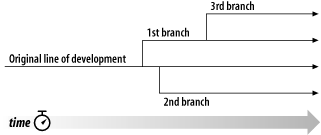
\includegraphics[keepaspectratio]{images/ch04dia1.png}}
\caption{Branches of development}\label{svn.branchmerge.whatis.dia-1}
\end{figure}

Subversion has commands to help you maintain parallel branches of your
files and directories. It allows you to create branches by copying your
data, and remembers that the copies are related to one another. It also
helps you duplicate changes from one branch to another. Finally, it can
make portions of your working copy reflect different branches so that
you can ``mix and match'' different lines of development in your daily
work.

\section{Using Branches}\label{svn.branchmerge.using}

At this point, you should understand how each commit creates a new state
of the filesystem tree (called a ``revision'') in the repository. If you
don\textquotesingle t, go back and read about revisions in
\hyperref[svn.basic.in-action.revs]{Revisions}.

Let\textquotesingle s revisit the example from
\hyperref[svn.basic]{Fundamental Concepts}. Remember that you and your
collaborator, Sally, are sharing a repository that contains two
projects, \texttt{paint} and \texttt{calc}. Notice that in
\hyperref[svn.branchmerge.using.dia-1]{Starting repository layout},
however, each project directory now contains subdirectories named
\texttt{trunk} and \texttt{branches}. The reason for this will soon
become clear.

\begin{figure}
\centering
\pandocbounded{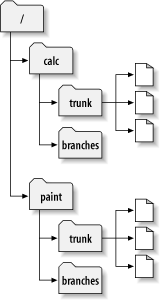
\includegraphics[keepaspectratio]{images/ch04dia2.png}}
\caption{Starting repository layout}\label{svn.branchmerge.using.dia-1}
\end{figure}

As before, assume that Sally and you both have working copies of the
``calc'' project. Specifically, you each have a working copy of
\texttt{/calc/trunk}. All the files for the project are in this
subdirectory rather than in \texttt{/calc} itself, because your team has
decided that \texttt{/calc/trunk} is where the ``main line'' of
development is going to take place.

Let\textquotesingle s say that you\textquotesingle ve been given the
task of implementing a large software feature. It will take a long time
to write, and will affect all the files in the project. The immediate
problem is that you don\textquotesingle t want to interfere with Sally,
who is in the process of fixing small bugs here and there.
She\textquotesingle s depending on the fact that the latest version of
the project (in \texttt{/calc/trunk}) is always usable. If you start
committing your changes bit by bit, you\textquotesingle ll surely break
things for Sally (and other team members as well).

One strategy is to crawl into a hole: you can stop sharing information
for a week or two, gutting and reorganizing all the files in your
private working copy but not committing or updating until
you\textquotesingle re completely finished with your task. There are a
number of problems with this, though. First, it\textquotesingle s not
very safe. Should something bad happen to your working copy or computer,
you risk losing all your changes. Second, it\textquotesingle s not very
flexible. Unless you manually replicate your changes across different
working copies or computers, you\textquotesingle re stuck trying to make
your changes in a single working copy. Similarly, it\textquotesingle s
difficult to share your work-in-progress with anyone else. A common
software development ``best practice'' is to allow your peers to review
your work as you go. If nobody sees your intermediate commits, you lose
potential feedback and may end up going down the wrong path for weeks
before another person on your team notices. Finally, when
you\textquotesingle re finished with all your changes, you might find it
very difficult to merge your completed work with the rest of the
company\textquotesingle s main body of code. Sally (or others) may have
made many other changes in the repository that are difficult to
incorporate into your working copy when you eventually run
\texttt{svn\ update} after weeks of isolation.

The better solution is to create your own branch, or line of
development, in the repository. This allows you to save your
not-yet-completed work frequently without interfering with
others\textquotesingle{} changes and while still selectively sharing
information with your collaborators. You\textquotesingle ll see exactly
how this works as we continue.

\subsection{Creating a Branch}\label{svn.branchmerge.using.create}

Creating a branch is very simple---you make a copy of your project tree
in the repository using the \texttt{svn\ copy} command. Since your
project\textquotesingle s source code is rooted in the
\texttt{/calc/trunk} directory, it\textquotesingle s that directory that
you\textquotesingle ll copy. Where should the new copy live? Wherever
you wish. The repository location in which branches are stashed is left
by Subversion as a matter of project policy. Finally, your branch will
need a name to distinguish it from other branches. Once again, the name
you choose is unimportant to Subversion---you can use whatever name
works best for you and your team.

Let\textquotesingle s assume that your team (like most) has a policy of
creating branches in the \texttt{branches} directory that is a sibling
of the project\textquotesingle s trunk (the \texttt{/calc/branches}
directory in our scenario). Lacking inspiration, you settle on
\texttt{my-calc-branch} as the name you wish to give your branch. This
means that you\textquotesingle ll create a new directory,
\texttt{/calc/branches/my-calc-branch}, which begins its life as a copy
of \texttt{/calc/trunk}.

You may already have seen \texttt{svn\ copy} used to copy one file to
another within a working copy. But it can also be used to do a remote
copy---a copy that immediately results in a newly committed repository
revision and for which no working copy is required at all. Just copy one
URL to another:

\begin{verbatim}
$ svn copy ^/calc/trunk ^/calc/branches/my-calc-branch \
           -m "Creating a private branch of /calc/trunk."

Committed revision 341.
$
\end{verbatim}

This command causes a near-instantaneous commit in the repository,
creating a new directory in revision 341. The new directory is a copy of
\texttt{/calc/trunk}. This is shown in
\hyperref[svn.branchmerge.using.create.dia-1]{Repository with new
copy}.\footnote{Subversion does not support copying between different
  repositories. When using URLs with \texttt{svn\ copy} or
  \texttt{svn\ move}, you can only copy items within the same
  repository.} While it\textquotesingle s also possible to create a
branch by using \texttt{svn\ copy} to duplicate a directory within the
working copy, this technique isn\textquotesingle t recommended. It can
be quite slow, in fact! Copying a directory on the client side is a
linear-time operation, in that it actually has to duplicate every file
and subdirectory within that working copy directory on the local disk.
Copying a directory on the server, however, is a constant-time
operation, and it\textquotesingle s the way most people create branches.
In addition, this practice raises the possibility of copying
mixed-revision working copies. This isn\textquotesingle t inherently
dangerous, but can cause unnecessary complications later during merging.
If you do choose to create a branch by copying a working copy path, you
should be sure the source directory has no local modifications and is
not at mixed-revisions.

\begin{figure}
\centering
\pandocbounded{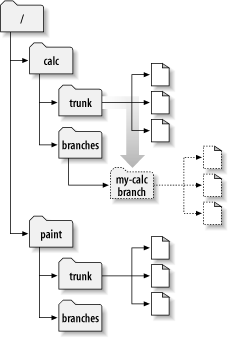
\includegraphics[keepaspectratio]{images/ch04dia3.png}}
\caption{Repository with new
copy}\label{svn.branchmerge.using.create.dia-1}
\end{figure}

Cheap Copies

Subversion\textquotesingle s repository has a special design. When you
copy a directory, you don\textquotesingle t need to worry about the
repository growing huge---Subversion doesn\textquotesingle t actually
duplicate any data. Instead, it creates a new directory entry that
points to an \emph{existing} tree. If you\textquotesingle re an
experienced Unix user, you\textquotesingle ll recognize this as the same
concept behind a hard link. As further changes are made to files and
directories beneath the copied directory, Subversion continues to employ
this hard link concept where it can. It duplicates data only when it is
necessary to disambiguate different versions of objects.

This is why you\textquotesingle ll often hear Subversion users talk
about ``cheap copies.'' It doesn\textquotesingle t matter how large the
directory is---it takes a very tiny, constant amount of time and space
to make a copy of it. In fact, this feature is the basis of how commits
work in Subversion: each revision is a ``cheap copy'' of the previous
revision, with a few items lazily changed within. (To read more about
this, visit Subversion\textquotesingle s web site and read about the
``bubble up'' method in Subversion\textquotesingle s design documents.)

Of course, these internal mechanics of copying and sharing data are
hidden from the user, who simply sees copies of trees. The main point
here is that copies are cheap, both in time and in space. If you create
a branch entirely within the repository (by running
\texttt{svn\ copy\ URL1\ URL2}), it\textquotesingle s a quick,
constant-time operation. Make branches as often as you want.

\subsection{Working with Your Branch}\label{svn.branchmerge.using.work}

Now that you\textquotesingle ve created a branch of the project, you can
check out a new working copy to start using it:

\begin{verbatim}
$ svn checkout http://svn.example.com/repos/calc/branches/my-calc-branch
A    my-calc-branch/doc
A    my-calc-branch/src
A    my-calc-branch/doc/INSTALL
A    my-calc-branch/src/real.c
A    my-calc-branch/src/main.c
A    my-calc-branch/src/button.c
A    my-calc-branch/src/integer.c
A    my-calc-branch/Makefile
A    my-calc-branch/README
Checked out revision 341.

$
\end{verbatim}

There\textquotesingle s nothing special about this working copy; it
simply mirrors a different directory in the repository. When you commit
changes, however, Sally won\textquotesingle t see them when she updates,
because her working copy is of \texttt{/calc/trunk}. (Be sure to read
\hyperref[svn.branchmerge.switchwc]{Traversing Branches} later in this
chapter: the \texttt{svn\ switch} command is an alternative way of
creating a working copy of a branch.)

Let\textquotesingle s pretend that a week goes by, and the following
commits happen:

\begin{itemize}
\item
  You make a change to
  \texttt{/calc/branches/my-calc-branch/src/button.c}, which creates
  revision 342.
\item
  You make a change to
  \texttt{/calc/branches/my-calc-branch/src/integer.c}, which creates
  revision 343.
\item
  Sally makes a change to \texttt{/calc/trunk/src/integer.c}, which
  creates revision 344.
\end{itemize}

Now two independent lines of development (shown in
\hyperref[svn.branchmerge.using.work.dia-1]{The branching of one
file\textquotesingle s history}) are happening on \texttt{integer.c}.

\begin{figure}
\centering
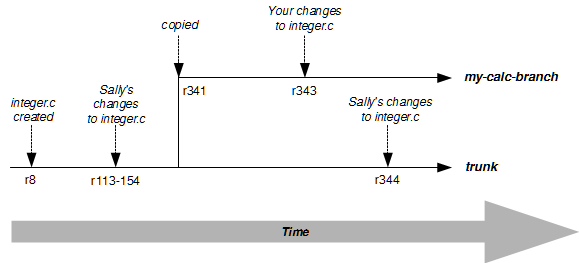
\includegraphics[width=4.81in,height=2.18in]{images/basic-branch.png}
\caption{The branching of one file\textquotesingle s
history}\label{svn.branchmerge.using.work.dia-1}
\end{figure}

Things get interesting when you look at the history of changes made to
your copy of \texttt{integer.c}:

\begin{verbatim}
$ pwd
/home/user/my-calc-branch

$ svn log -v src/integer.c
------------------------------------------------------------------------
r343 | user | 2013-02-15 14:11:09 -0500 (Fri, 15 Feb 2013) | 1 line
Changed paths:
   M /calc/branches/my-calc-branch/src/integer.c

* integer.c:  frozzled the wazjub.
------------------------------------------------------------------------
r341 | user | 2013-02-15 07:41:25 -0500 (Fri, 15 Feb 2013) | 1 line
Changed paths:
   A /calc/branches/my-calc-branch (from /calc/trunk:340)

Creating a private branch of /calc/trunk.
------------------------------------------------------------------------
r154 | sally | 2013-01-30 04:20:03 -0500 (Wed, 30 Jan 2013) | 2 lines
Changed paths:
   M /calc/trunk/src/integer.c

* integer.c:  changed a docstring.
------------------------------------------------------------------------
…
------------------------------------------------------------------------
r113 | sally | 2013-01-26 15:50:21 -0500 (Sat, 26 Jan 2013) | 2 lines
Changed paths:
   M /calc/trunk/src/integer.c

* integer.c: Revise the fooplus API.
------------------------------------------------------------------------
r8 | sally | 2013-01-17 16:55:36 -0500 (Thu, 17 Jan 2013) | 1 line
Changed paths:
   A /calc/trunk/Makefile
   A /calc/trunk/README
   A /calc/trunk/doc/INSTALL
   A /calc/trunk/src/button.c
   A /calc/trunk/src/integer.c
   A /calc/trunk/src/main.c
   A /calc/trunk/src/real.c

Initial trunk code import for calc project.
------------------------------------------------------------------------
\end{verbatim}

Notice that Subversion is tracing the history of your
branch\textquotesingle s \texttt{integer.c} all the way back through
time, even traversing the point where it was copied. It shows the
creation of the branch as an event in the history, because
\texttt{integer.c} was implicitly copied when all of
\texttt{/calc/trunk/} was copied. Now look at what happens when Sally
runs the same command on her copy of the file:

\begin{verbatim}
$ pwd
/home/sally/calc

$ svn log -v src/integer.c
------------------------------------------------------------------------
r344 | sally | 2013-02-15 16:44:44 -0500 (Fri, 15 Feb 2013) | 1 line
Changed paths:
   M /calc/trunk/src/integer.c

Refactor the bazzle functions.
------------------------------------------------------------------------
r154 | sally | 2013-01-30 04:20:03 -0500 (Wed, 30 Jan 2013) | 2 lines
Changed paths:
   M /calc/trunk/src/integer.c

* integer.c:  changed a docstring.
------------------------------------------------------------------------
…
------------------------------------------------------------------------
r113 | sally | 2013-01-26 15:50:21 -0500 (Sat, 26 Jan 2013) | 2 lines
Changed paths:
   M /calc/trunk/src/integer.c

* integer.c: Revise the fooplus API.
------------------------------------------------------------------------
r8 | sally | 2013-01-17 16:55:36 -0500 (Thu, 17 Jan 2013) | 1 line
Changed paths:
   A /calc/trunk/Makefile
   A /calc/trunk/README
   A /calc/trunk/doc/INSTALL
   A /calc/trunk/src/button.c
   A /calc/trunk/src/integer.c
   A /calc/trunk/src/main.c
   A /calc/trunk/src/real.c

Initial trunk code import for calc project.
------------------------------------------------------------------------
\end{verbatim}

Sally sees her own revision 344 change, but not the change you made in
revision 343. As far as Subversion is concerned, these two commits
affected different files in different repository locations. However,
Subversion \emph{does} show that the two files share a common history.
Before the branch copy was made in revision 341, the files used to be
the same file. That\textquotesingle s why you and Sally both see the
changes made between revisions 8 and 154.

\subsection{The Key Concepts Behind
Branching}\label{svn.branchmerge.using.concepts}

You should remember two important lessons from this section. First,
Subversion has no internal concept of a branch---it knows only how to
make copies. When you copy a directory, the resultant directory is only
a ``branch'' because \emph{you} attach that meaning to it. You may think
of the directory differently, or treat it differently, but to Subversion
it\textquotesingle s just an ordinary directory that happens to carry
some extra historical information.

Second, because of this copy mechanism, Subversion\textquotesingle s
branches exist as \emph{normal filesystem directories} in the
repository. This is different from other version control systems, where
branches are typically defined by adding extra-dimensional ``labels'' to
collections of files. The location of your branch directory
doesn\textquotesingle t matter to Subversion. Most teams follow a
convention of putting all branches into a \texttt{/branches} directory,
but you\textquotesingle re free to invent any policy you wish.

\section{Basic Merging}\label{svn.branchmerge.basicmerging}

Now you and Sally are working on parallel branches of the project:
you\textquotesingle re working on a private branch, and Sally is working
on the trunk, or main line of development.

For projects that have a large number of contributors,
it\textquotesingle s common for most people to have working copies of
the trunk. Whenever someone needs to make a long-running change that is
likely to disrupt the trunk, a standard procedure is to create a private
branch and commit changes there until all the work is complete.

So, the good news is that you and Sally aren\textquotesingle t
interfering with each other. The bad news is that it\textquotesingle s
very easy to drift \emph{too} far apart. Remember that one of the
problems with the ``crawl in a hole'' strategy is that by the time
you\textquotesingle re finished with your branch, it may be
near-impossible to merge your changes back into the trunk without a huge
number of conflicts.

Instead, you and Sally might continue to share changes as you work.
It\textquotesingle s up to you to decide which changes are worth
sharing; Subversion gives you the ability to selectively ``copy''
changes between branches. And when you\textquotesingle re completely
finished with your branch, your entire set of branch changes can be
copied back into the trunk. In Subversion terminology, the general act
of replicating changes from one branch to another is called merging, and
it is performed using various invocations of the \texttt{svn\ merge}
subcommand.

In the examples that follow, we\textquotesingle re assuming that both
your Subversion client and server are running Subversion 1.8 (or later).
If either client or server is older than version 1.5, things are more
complicated: the system won\textquotesingle t track changes
automatically, forcing you to use painful manual methods to achieve
similar results. That is, you\textquotesingle ll always need to use the
detailed merge syntax to specify specific ranges of revisions to
replicate (see \hyperref[svn.branchmerge.advanced.advancedsyntax]{Merge
Syntax: Full Disclosure} later in this chapter), and take special care
to keep track of what\textquotesingle s already been merged and what
hasn\textquotesingle t. For this reason, we \emph{strongly} recommend
that you make sure your client and server are at least at version 1.5.

\protect\phantomsection\label{svn.branchmerge.basicmerging.mergetracking}
Merge Tracking

Subversion 1.5 introduced the merge tracking feature to Subversion.
Prior to this feature keeping track of merges required cumbersome manual
procedures or the use of external tools. Subsequent releases of
Subversion introduced many enhancements and bug fixes to merge tracking,
which is why we recommend using the most recent versions for both your
server and client. Keep in mind that even if your server is running
1.5-1.7, you can still use a 1.8 client. This is particularly important
with regard to merge tracking, because the overwhelming majority of
fixes and enhancements to it are on the client side.

\subsection{Changesets}\label{svn.branchmerge.changesets}

Before we proceed further, we should warn you that
there\textquotesingle s a lot of discussion of ``changes'' in the pages
ahead. A lot of people experienced with version control systems use the
terms ``change'' and ``changeset'' interchangeably, and we should
clarify what Subversion understands as a changeset.

Everyone seems to have a slightly different definition of changeset, or
at least a different expectation of what it means for a version control
system to have one. For our purposes, let\textquotesingle s say that a
changeset is just a collection of changes with a unique name. The
changes might include textual edits to file contents, modifications to
tree structure, or tweaks to metadata. In more common speak, a changeset
is just a patch with a name you can refer to.

In Subversion, a global revision number \textless N\textgreater{} names
a tree in the repository: it\textquotesingle s the way the repository
looked after the \textless N\textgreater th commit. It\textquotesingle s
also the name of an implicit changeset: if you compare tree
\textless N\textgreater{} with tree \textless N\textgreater-1, you can
derive the exact patch that was committed. For this reason,
it\textquotesingle s easy to think of revision \textless N\textgreater{}
as not just a tree, but a changeset as well. If you use an issue tracker
to manage bugs, you can use the revision numbers to refer to particular
patches that fix bugs---for example, ``this issue was fixed by r9238.''
Somebody can then run \texttt{svn\ log\ -r\ 9238} to read about the
exact changeset that fixed the bug, and run \texttt{svn\ diff\ -c\ 9238}
to see the patch itself. And (as you\textquotesingle ll see shortly)
Subversion\textquotesingle s \texttt{svn\ merge} command is able to use
revision numbers. You can merge specific changesets from one branch to
another by naming them in the merge arguments: passing \texttt{-c\ 9238}
to \texttt{svn\ merge} would merge changeset r9238 into your working
copy.

\subsection{Keeping a Branch in
Sync}\label{svn.branchmerge.basicmerging.stayinsync}

Continuing with our running example, let\textquotesingle s suppose that
a week has passed since you started working on your private branch. Your
new feature isn\textquotesingle t finished yet, but at the same time you
know that other people on your team continue to make important changes
in the project\textquotesingle s \texttt{/trunk}. It\textquotesingle s
in your best interest to replicate those changes to your own branch,
just to make sure they mesh well with your changes. This is done by
performing an automatic sync merge---a merge operation designed to bring
your branch up to date with any changes made to its ancestral parent
branch since your branch was created. An ``automatic'' merge is simply
one in which you provide the bare minimum of information required for a
merge (i.e. a single merge source and a working copy target) and let
Subversion determine which changes need merging---no changesets are
passed to \texttt{svn\ merge} via the \texttt{-r} or \texttt{-c} options
in an automatic merge.

Frequently keeping your branch in sync with the main development line
helps prevent ``surprise'' conflicts when the time comes for you to fold
your changes back into the trunk.

Subversion is aware of the history of your branch and knows when it
split away from the trunk. To perform a sync merge, first make sure your
working copy of the branch is ``clean''---that it has no local
modifications reported by \texttt{svn\ status}. Then simply run:

\begin{verbatim}
$ pwd
/home/user/my-calc-branch

$ svn merge ^/calc/trunk
--- Merging r341 through r351 into '.':
U    doc/INSTALL
U    src/real.c
U    src/button.c
U    Makefile
--- Recording mergeinfo for merge of r341 through r351 into '.':
 U   .
 $
\end{verbatim}

This basic syntax---\texttt{svn\ merge\ URL}---tells Subversion to merge
all changes which have not been previously merged from the URL to the
current working directory (which is typically the root of your working
copy). Notice that we\textquotesingle re using the caret (\texttt{\^{}})
syntax\footnote{This was introduced in svn 1.6.} to avoid having to type
out the entire \texttt{/trunk} URL. Also note the ``Recording mergeinfo
for merge\ldots{}'' notification. This tells you that the merge is
updating the \texttt{svn:mergeinfo} property. We\textquotesingle ll
discuss both this property and these notifications later in this
chapter, in \hyperref[svn.branchmerge.basicmerging.mergeinfo]{Mergeinfo
and Previews}.

In this book and elsewhere (Subversion mailing lists, articles on merge
tracking, etc.) you will frequently come across the term mergeinfo. This
is simply shorthand for the \texttt{svn:mergeinfo} property.

Keeping a Branch in Sync Without Merge Tracking

You may not always be able to use Subversion\textquotesingle s merge
tracking feature, perhaps because your server is running Subversion 1.4
or earlier or you must use an older client. In such a scenario, you can
of course still perform merges, but Subversion will need you to manually
do many of the historical calculations that it automatically does on
your behalf when the merge tracking feature is available.

To replicate the most recent trunk changes you need to perform sync
merges the ``old-fashioned'' way---by specifying ranges of revisions you
wish to merge.

Using the ongoing example, you know that you branched
\texttt{/calc/trunk} to \texttt{/calc/branches/my-calc-branch} in
revision 341:

\begin{verbatim}
$ svn log -v -r341
------------------------------------------------------------------------
r341 | user | 2013-02-15 07:41:25 -0500 (Fri, 15 Feb 2013) | 1 line
Changed paths:
   A /calc/branches/my-calc-branch (from /calc/trunk:340)

Creating a private branch of /calc/trunk.
------------------------------------------------------------------------
\end{verbatim}

When you are ready to synchronize your branch with the ongoing changes
from trunk, you specify the starting revision as the revision of
\texttt{/calc/trunk} which the branch was copied from and the ending
revision as the youngest change on \texttt{/calc/trunk}. You can find
the latter with the \texttt{svn\ log} command with the \texttt{-r} set
to \texttt{HEAD}:

\begin{verbatim}
$ svn log -q -rHEAD http://svn.example.com/repos/calc/trunk
------------------------------------------------------------------------
r351 | sally | 2013-02-16 08:04:22 -0500 (Sat, 16 Feb 2013)
------------------------------------------------------------------------

$ svn merge http://svn.example.com/repos/calc/trunk -r340:351
U    doc/INSTALL
U    src/real.c
U    src/button.c
U    Makefile
\end{verbatim}

After any conflicts have been resolved, you can commit the merged
changes to your branch. Now, to avoid accidentally trying to merge these
same changes into your branch again in the future,
you\textquotesingle ll need to record the fact that
you\textquotesingle ve already merged them. But where should that record
be kept? One of the simplest places to record this information is in the
log message for the commit of the merge:

\begin{verbatim}
$ svn ci -m "Sync the my-calc-branch with ^/calc/trunk through r351."
…
\end{verbatim}

The next time you sync \texttt{/calc/branches/my-calc-branch} with
\texttt{/calc/trunk} you repeat this process, except that the starting
revision is the \emph{youngest} revision that\textquotesingle s already
been merged in from the trunk. If you\textquotesingle ve been keeping
good records of your merges in the commit log messages, you should be
able to determine what that youngest revision was by reading the
revision logs associated with your branch. Once you know your starting
revision, you can perform another sync merge:

\begin{verbatim}
$ svn log -q -rHEAD http://svn.example.com/repos/calc/trunk
------------------------------------------------------------------------
r959 | sally | 2013-03-5 7:30:21 -0500 (Tue, 05 Mar 2013)
------------------------------------------------------------------------

$ svn merge http://svn.example.com/repos/calc/trunk -r351:959
…
\end{verbatim}

After running the prior example, your branch working copy now contains
new local modifications, and these edits are duplications of all of the
changes that have happened on the trunk since you first created your
branch:

\begin{verbatim}
$ svn status
 M      .
M       Makefile
M       doc/INSTALL
M       src/button.c
M       src/real.c
\end{verbatim}

At this point, the wise thing to do is look at the changes carefully
with \texttt{svn\ diff}, and then build and test your branch. Notice
that the current working directory (``\texttt{.}'') has also been
modified; \texttt{svn\ diff} shows that its \texttt{svn:mergeinfo}
property has been created.

\begin{verbatim}
$ svn diff --depth empty .
Index: .
===================================================================
--- .   (revision 351)
+++ .   (working copy)

Property changes on: .
___________________________________________________________________
Added: svn:mergeinfo
   Merged /calc/trunk:r341-351
\end{verbatim}

This new property is important merge-related metadata that you should
\emph{not} touch, since it is needed by future \texttt{svn\ merge}
commands. (We\textquotesingle ll learn more about this metadata later in
the chapter.)

After performing the merge, you might also need to resolve some
conflicts---just as you do with \texttt{svn\ update}---or possibly make
some small edits to get things working properly. (Remember, just because
there are no \emph{syntactic} conflicts doesn\textquotesingle t mean
there aren\textquotesingle t any \emph{semantic} conflicts!) If you
encounter serious problems, you can always abort the local changes by
running \texttt{svn\ revert\ .\ -R} (which will undo all local
modifications) and starting a long ``what\textquotesingle s going on?''
discussion with your collaborators. If things look good, however, you
can submit these changes into the repository:

\begin{verbatim}
$ svn commit -m "Sync latest trunk changes to my-calc-branch."
Sending        .
Sending        Makefile
Sending        doc/INSTALL
Sending        src/button.c
Sending        src/real.c
Transmitting file data ....
Committed revision 352.
\end{verbatim}

At this point, your private branch is now ``in sync'' with the trunk, so
you can rest easier knowing that as you continue to work in isolation,
you\textquotesingle re not drifting too far away from what everyone else
is doing.

Why Not Use Patches Instead?

A question may be on your mind, especially if you\textquotesingle re a
Unix user: why bother to use \texttt{svn\ merge} at all? Why not simply
use \texttt{svn\ patch} or the operating system\textquotesingle s
\texttt{patch} command to accomplish the same job? For example:

\begin{verbatim}
$ cd my-calc-branch

$ svn diff -r 341:351 ^/calc/trunk > my-patch-file

$ svn patch my-patch-file
U         doc/INSTALL
U         src/real.c
U         src/button.c
U         Makefile
\end{verbatim}

In this particular example, there really isn\textquotesingle t much
difference. But \texttt{svn\ merge} has special abilities that surpass
the \texttt{patch} program. The file format used by \texttt{patch} is
quite limited; it\textquotesingle s able to tweak file contents only.
There\textquotesingle s no way to represent changes to \emph{trees},
such as the addition, removal, or renaming of files and directories. Nor
can the \texttt{patch} program notice changes to properties. If
Sally\textquotesingle s change had, say, added a new directory, the
output of \texttt{svn\ diff} wouldn\textquotesingle t have mentioned it
at all. \texttt{svn\ diff} outputs only the limited patch format, so
there are some ideas it simply can\textquotesingle t express. Even
Subversion\textquotesingle s own \texttt{svn\ patch} subcommand, while
more flexible than the \texttt{patch} program, still has similar
limitations.

The \texttt{svn\ merge} command, however, can express changes in tree
structure and properties by directly applying them to your working copy.
Even more important, this command records the changes that have been
duplicated to your branch so that Subversion is aware of exactly which
changes exist in each location (see
\hyperref[svn.branchmerge.basicmerging.mergeinfo]{Mergeinfo and
Previews}). This is a critical feature that makes branch management
usable; without it, users would have to manually keep notes on which
sets of changes have or haven\textquotesingle t been merged yet.

Suppose that another week has passed. You\textquotesingle ve committed
more changes to your branch, and your comrades have continued to improve
the trunk as well. Once again, you want to replicate the latest trunk
changes to your branch and bring yourself in sync. Just run the same
merge command again!

\begin{verbatim}
$ svn merge ^/calc/trunk
svn: E195020: Cannot merge into mixed-revision working copy [352:357]; try up\
dating first
$
\end{verbatim}

Well that was unexpected! After making changes to your branch over the
past week you now find yourself with a working copy that contains a
mixture of revisions (see
\hyperref[svn.basic.in-action.mixedrevs]{Mixed-revision working
copies}). With Subversion 1.7 and later, the \texttt{svn\ merge}
subcommand disables merges into mixed-revision working copies by
default. Without going into too much detail, this is because of
limitations in the way merges are tracked by the \texttt{svn:mergeinfo}
property (see
\hyperref[svn.branchmerge.basicmerging.mergeinfo]{Mergeinfo and
Previews} for details). These limitations mean that merges into
mixed-revision working copies can result in unexpected text and tree
conflicts.\footnote{The \texttt{svn\ merge} subcommand option
  \texttt{-\/-allow-mixed-revisions} allows you to override this
  prohibition, but you should only do so if you understand the
  ramifications and have a good reason for it.} We don\textquotesingle t
want any needless conflicts, so we update the working copy and then
reattempt the merge.

\begin{verbatim}
$ svn up
Updating '.':
At revision 361.

$ svn merge ^/calc/trunk
--- Merging r352 through r361 into '.':
U    src/real.c
U    src/main.c
--- Recording mergeinfo for merge of r352 through r361 into '.':
 U   .
\end{verbatim}

Subversion knows which trunk changes you previously replicated to your
branch, so it carefully replicates only those changes you
don\textquotesingle t yet have. And once again, you build, test, and
\texttt{svn\ commit} the local modifications to your branch.

\subsection{Subtree Merges and Subtree
Mergeinfo}\label{svn.branchmerge.basicmerging.stayinsync.subtree}

In most of the examples in this chapter the merge target is the root
directory of a branch (see
\hyperref[svn.branchmerge.whatis]{What\textquotesingle s a Branch?}).
While this is a best practice, you may occasionally need to merge
directly to some child of the branch root. This type of merge is called
a subtree merge and the mergeinfo recorded to describe it is called
subtree mergeinfo. There is nothing special about subtree merges or
subtree mergeinfo. In fact there is really only one important point to
keep in mind about these concepts: the complete record of merges to a
branch may not be contained solely in the mergeinfo on the branch root.
You may have to consider subtree mergeinfo to get a full accounting.
Fortunately Subversion does this for you and rarely will you need to
concern yourself with it. A brief example will help explain:

\begin{verbatim}
# We need to merge r958 from trunk to branches/proj-X/doc/INSTALL,
# but that revision also affects main.c, which we don't want to merge:
$ svn log --verbose --quiet -r 958 ^/
------------------------------------------------------------------------
r958 | bruce | 2011-10-20 13:28:11 -0400 (Thu, 20 Oct 2011)
Changed paths:
   M /trunk/doc/INSTALL
   M /trunk/src/main.c
------------------------------------------------------------------------

# No problem, we'll do a subtree merge targeting the INSTALL file
# directly, but first take a note of what mergeinfo exists on the
# root of the branch:
$ cd branches/proj-X

$ svn propget svn:mergeinfo --recursive
Properties on '.':
  svn:mergeinfo
    /trunk:651-652

# Now we perform the subtree merge, note that merge source
# and target both point to INSTALL:
$ svn merge ^/trunk/doc/INSTALL doc/INSTALL -c 958
--- Merging r958 into 'doc/INSTALL':
U    doc/INSTALL
--- Recording mergeinfo for merge of r958 into 'doc/INSTALL':
 G   doc/INSTALL

# Once the merge is complete there is now subtree mergeinfo on INSTALL:
$ svn propget svn:mergeinfo --recursive
Properties on '.':
  svn:mergeinfo
    /trunk:651-652
Properties on 'doc/INSTALL':
  svn:mergeinfo
    /trunk/doc/INSTALL:651-652,958

# What if we then decide we do want all of r958? Easy, all we need do is
# repeat the merge of that revision, but this time to the root of the
# branch, Subversion notices the subtree mergeinfo on INSTALL and doesn't
# try to merge any changes to it, only the changes to main.c are merged:
$ svn merge ^/subversion/trunk . -c 958
--- Merging r958 into '.':
U    src/main.c
--- Recording mergeinfo for merge of r958 into '.':
 U   .
--- Eliding mergeinfo from 'doc/INSTALL':
 U   doc/INSTALL
\end{verbatim}

You might be wondering why \texttt{INSTALL} in the above example has
mergeinfo for r651-652, when we only merged r958. This is due to
mergeinfo inheritance, which we\textquotesingle ll cover in the sidebar
\hyperref[svn.branchmerge.basicmerging.mergeinfo.inheritance]{Mergeinfo
Inheritance}. Also note that the subtree mergeinfo on
\texttt{doc/INSTALL} was removed, or ``elided''. This is called
mergeinfo elision and it occurs whenever Subversion detects redundant
subtree mergeinfo.

Prior to Subversion 1.7, merges unconditionally updated \emph{all} of
the subtree mergeinfo under the target to describe the merge. For users
with a lot of subtree mergeinfo this meant that relatively ``simple''
merges (e.g. one which applied a diff to only a single file) resulted in
changes to every subtree with mergeinfo, even those that were not
parents of the affected path(s). This caused some level of confusion and
frustration. Subversion 1.7 and later addresses this problem by only
updating the mergeinfo on subtrees which are parents of the paths
modified by the merge (i.e. paths changed, added, or deleted by
application of the difference, see
\hyperref[svn.branchmerge.advanced.advancedsyntax]{Merge Syntax: Full
Disclosure}). The one exception to this behavior regards the actual
merge target; the merge target\textquotesingle s mergeinfo is always
updated to describe the merge, even if the applied difference made no
changes.

\subsection{Reintegrating a
Branch}\label{svn.branchmerge.basicmerging.reintegrate}

What happens when you finally finish your work, though? Your new feature
is done, and you\textquotesingle re ready to merge your branch changes
back to the trunk (so your team can enjoy the bounty of your labor). The
process is simple. First, bring your branch into sync with the trunk
again, just as you\textquotesingle ve been doing all along\footnote{Since
  Subversion 1.7 you don\textquotesingle t absolutely have to do all
  your sync merges to the root of your branch as we do in this example.
  \emph{If} your branch is effectively synced via a series of subtree
  merges then the reintegrate will work, but ask yourself, if the branch
  is effectively synced, then why are you doing subtree merges? Doing so
  is almost always needlessly complex.}:

\begin{verbatim}
$ svn up # (make sure the working copy is up to date)
Updating '.':
At revision 378.

$ svn merge ^/calc/trunk
--- Merging r362 through r378 into '.':
U    src/main.c
--- Recording mergeinfo for merge of r362 through r378 into '.':
 U   .

$ # build, test, ...

$ svn commit -m "Final merge of trunk changes to my-calc-branch."
Sending        .
Sending        src/main.c
Transmitting file data .
Committed revision 379.
\end{verbatim}

Now, use \texttt{svn\ merge} subcommand to automatically replicate your
branch changes back into the trunk. This type of merge is called an
``automatic reintegrate'' merge. You\textquotesingle ll need a working
copy of \texttt{/calc/trunk}. You can get one by doing an
\texttt{svn\ checkout}, dredging up an old trunk working copy from
somewhere on your disk, or using \texttt{svn\ switch} (see
\hyperref[svn.branchmerge.switchwc]{Traversing Branches}).

The term ``reintegrating'' comes from the \texttt{merge} option
\texttt{-\/-reintegrate}. This option is deprecated in Subversion 1.8
(which automatically detects when a reintegrate merge is needed), but is
required for Subversion 1.5 through 1.7 clients when performing
reintegrate merges.

Your trunk working copy cannot have any local edits, switched paths, or
contain a mixture of revisions (see
\hyperref[svn.basic.in-action.mixedrevs]{Mixed-revision working
copies}). While these are typically best practices for merging anyway,
they are \emph{required} for automatic reintegrate merges.

Once you have a clean working copy of the trunk, you\textquotesingle re
ready to merge your branch back into it:

\begin{verbatim}
$ pwd
/home/user/calc-trunk

$ svn update
Updating '.':
At revision 379.

$ svn merge ^/calc/branches/my-calc-branch
--- Merging differences between repository URLs into '.':
U    src/real.c
U    src/main.c
U    Makefile
--- Recording mergeinfo for merge between repository URLs into '.':
 U   .

$ # build, test, verify, ...

$ svn commit -m "Merge my-calc-branch back into trunk!"
Sending        .
Sending        Makefile
Sending        src/main.c
Sending        src/real.c
Transmitting file data ...
Committed revision 380.
\end{verbatim}

Congratulations, your branch-specific changes have now been merged back
into the main line of development. Notice that the automatic reintegrate
merge did a different sort of work than what you\textquotesingle ve done
up until now. Previously, we were asking \texttt{svn\ merge} to grab the
``next set'' of changes from one line of development (the trunk) and
duplicate them to another (your branch). This is fairly straightforward,
and each time Subversion knows how to pick up where it left off. In our
prior examples, you can see that first it merges the ranges 341:351 from
\texttt{/calc/trunk} to \texttt{/calc/branches/my-calc-branch}; later
on, it continues by merging the next contiguously available range,
351:361. When doing the final sync, it merges the range 361:378.

When merging \texttt{/calc/branches/my-calc-branch} back to the
\texttt{/calc/trunk}, however, the underlying mathematics are quite
different. Your feature branch is now a mishmash of both duplicated
trunk changes and private branch changes, so there\textquotesingle s no
simple contiguous range of revisions to copy over. By using an automatic
merge, you\textquotesingle re asking Subversion to carefully replicate
\emph{only} those changes unique to your branch. (And in fact, it does
this by comparing the latest trunk tree with the latest branch tree: the
resulting difference is exactly your branch changes!)

Keep in mind that the automatic reintegrate merges only support the use
case described above. Because of this narrow focus, in addition to the
requirements previously mentioned (up-to-date working copy \footnote{Automatic
  reintegrate merges are allowed if the target is a shallow checkout
  (see \hyperref[svn.advanced.sparsedirs]{Sparse Directories}) but any
  paths affected by the diff which are ``missing'' due to the sparse
  working copy will be skipped---this is probably \emph{not} what you
  intended!} with no mixed-revisions, switched paths or local changes)
it will not function in combination with most of the other
\texttt{svn\ merge} options. You\textquotesingle ll get an error if you
use any non-global options but these: \texttt{-\/-accept},
\texttt{-\/-dry-run}, \texttt{-\/-diff3-cmd}, \texttt{-\/-extensions},
or \texttt{-\/-quiet}.

Now that your private branch is merged to trunk, you may wish to remove
it from the repository:

\begin{verbatim}
$ svn delete ^/calc/branches/my-calc-branch \
             -m "Remove my-calc-branch, reintegrated with trunk in r381."
…
\end{verbatim}

But wait! Isn\textquotesingle t the history of that branch valuable?
What if somebody wants to audit the evolution of your feature someday
and look at all of your branch changes? No need to worry. Remember that
even though your branch is no longer visible in the
\texttt{/calc/branches} directory, its existence is still an immutable
part of the repository\textquotesingle s history. A simple
\texttt{svn\ log} command on the \texttt{/calc/branches} URL will show
the entire history of your branch. Your branch can even be resurrected
at some point, should you desire (see
\hyperref[svn.branchmerge.basicmerging.resurrect]{Resurrecting Deleted
Items}).

If you choose not to delete your branch after reintegrating it to the
trunk you may continue to perform sync merges from the trunk and then
reintegrate the branch again\footnote{Only Subversion 1.8 supports this
  reuse of a feature branch. Earlier versions require some special
  handling before a feature branch can be reintegrated more than once.
  See the earlier version of this chapter for more information:
  \href{https://svnbook.red-bean.com/en/1.7/svn.branchmerge.basicmerging.html\#svn.branchemerge.basicmerging.reintegrate}{}}.
If you do this, only the changes made on your branch after the first
reintegrate are merged to the trunk.

\subsection{Mergeinfo and
Previews}\label{svn.branchmerge.basicmerging.mergeinfo}

The basic mechanism Subversion uses to track changesets---that is, which
changes have been merged to which branches---is by recording data in
versioned properties. Specifically, merge data is tracked in the
\texttt{svn:mergeinfo} property attached to files and directories. (If
you\textquotesingle re not familiar with Subversion properties, see
\hyperref[svn.advanced.props]{Properties}.)

You can examine the mergeinfo property, just like any other versioned
property:

\begin{verbatim}
$ cd my-calc-branch

$ svn pg svn:mergeinfo -v
Properties on '.':
  svn:mergeinfo
    /calc/trunk:341-378
\end{verbatim}

While it is possible to modify \texttt{svn:mergeinfo} just as you might
any other versioned property, we strongly discourage doing so unless you
\emph{really} know what you\textquotesingle re doing.

The amount of \texttt{svn:mergeinfo} on a single path can get quite
large, as can the output of a \texttt{svn\ propget\ -\/-recursive} or
\texttt{svn\ proplist\ -\/-recursive} when dealing with large amounts of
subtree mergeinfo. See
\hyperref[svn.branchmerge.basicmerging.stayinsync.subtree]{Subtree
Merges and Subtree Mergeinfo} . The formatted output produced by the
\texttt{-\/-verbose} option with either of these subcommands is often
very helpful in these cases.

The \texttt{svn:mergeinfo} property is automatically maintained by
Subversion whenever you run \texttt{svn\ merge}. Its value indicates
which changes made to a given path have been replicated into the
directory in question. In our previous example, the path which is the
source of the merged changes is \texttt{/calc/trunk} and the directory
which has received the changes is
\texttt{/calc/branches/my-calc-branch}. Earlier versions of Subversion
maintained the \texttt{svn:mergeinfo} property silently. You could still
detect the changes, after a merge completed, with the \texttt{svn\ diff}
or \texttt{svn\ status} subcommands, but the merge itself gave no
indication when it changed the \texttt{svn:mergeinfo} property. In
Subversion 1.7 and later this is no longer true as there are several
notifications to alert you when a merge updates the
\texttt{svn:mergeinfo} property. These notifications all begin with
``-\/-\/- Recording mergeinfo for'' and appear at the end of the merge.
Unlike other merge notifications, these don\textquotesingle t describe
the application of a difference to a working copy (see
\hyperref[svn.branchmerge.advanced.advancedsyntax]{Merge Syntax: Full
Disclosure}), but instead describe "housekeeping" changes made to keep
track of what was merged.

Subversion also provides a subcommand, \texttt{svn\ mergeinfo}, which is
helpful in seeing the merge relationships between two branches;
specifically which changesets a directory has absorbed or which
changesets it\textquotesingle s still eligible to receive. The latter
gives a sort of preview of which changes a subsequent
\texttt{svn\ merge} operation would replicate to your branch. By
default, \texttt{svn\ mergeinfo} gives an graphical overview of the
relationship between to branches. Returning to our earlier example, we
use the subcommand to analyze the relationship between
\texttt{/calc/trunk} and \texttt{/calc/branches/my-calc-branch}:

\begin{verbatim}
$ cd my-calc-branch

$ svn mergeinfo ^/calc/trunk
    youngest common ancestor
    |         last full merge
    |         |        tip of branch
    |         |        |         repository path

    340                382
    |                  |
  -------| |------------         calc/trunk
     \          /
      \        /
       --| |------------         calc/branches/my-calc-branch
              |        |
              379      382
\end{verbatim}

The diagram shows that \texttt{/calc/branches/my-calc-branch} was copied
from \texttt{/calc/trunk@340} and that most recent automatic merge was
the reintegrate merge we made from the branch to the trunk in r380.
Notice that the diagram does \emph{not} show the four automatic sync
merges we made in revisions 352, 362, 372, and 379. Only the most recent
automatic merge, in either direction\footnote{By ``direction'' we mean
  either trunk-to-branch (automatic sync) or branch-to-trunk (automatic
  reintegrate) merges.}, is shown. This default output is useful for
obtaining an overview of the merges between two branches, but to see the
specific revisions which were merged we use the
\texttt{-\/-show-revs=merged} option:

\begin{verbatim}
$ svn mergeinfo ^/calc/trunk --show-revs merged
r344
r345
r346
…
r366
r367
r368
\end{verbatim}

Likewise, to see which changes are eligible to merge from the trunk to
the branch we can use the \texttt{-\/-show-revs=eligible} option:

\begin{verbatim}
$ svn mergeinfo ^/calc/trunk --show-revs eligible
r380
r381
r382
\end{verbatim}

\protect\phantomsection\label{svn.branchmerge.basicmerging.mergeinfo.operativerevs}
Operative and Inoperative Merge Revisions

The revision lists produced by the \texttt{-\/-show-revs} option include
only revisions which made (or would make) changes when merged. So while
we have merged a contiguous range of revisions (i.e. r341-378) from
\texttt{/calc/trunk} to \texttt{/calc/branches/my-calc-branch}, only the
revisions listed with the \texttt{-\/-show-revs=merged} option actually
represent changes made on \texttt{/calc/trunk}. These revisions are
described as ``operative'' revisions as regards merging, not to be
confused with the operative revision used with the \texttt{-r} option,
see \hyperref[svn.advanced.pegrevs]{Peg and Operative Revisions}. Not
suprisingly, the revisions in the range r341-378 that are \emph{not}
listed as merged are termed ``inoperative'' revisions.

The \texttt{svn\ mergeinfo} command requires a ``source'' URL (where the
changes come from), and takes an optional ``target'' URL (where the
changes merge to). If no target URL is given, it assumes that the
current working directory is the target. In the prior example, because
we\textquotesingle re querying our branch working copy, the command
assumes we\textquotesingle re interested in receiving changes to
\texttt{/calc/branches/my-calc-branch} from the specified trunk URL.

Since Subversion 1.7, the \texttt{svn\ mergeinfo} subcommand can also
account for subtree mergeinfo and non-inheritable mergeinfo. It accounts
for subtree mergeinfo by use of the \texttt{-\/-recursive} or
\texttt{-\/-depth} options, while non-inheritable mergeinfo is
considered by default.

\protect\phantomsection\label{svn.branchmerge.basicmerging.mergeinfo.inheritance}
Mergeinfo Inheritance

When a path has the \texttt{svn:mergeinfo} property set on it we say it
has explicit mergeinfo. This explicit mergeinfo describes not only what
changes were merged into that particular directory, but also all the
children of that directory (because those children inherit the mergeinfo
of their parent path). For example:

\begin{verbatim}
# What explicit mergeinfo exists on a branch?
$ svn propget svn:mergeinfo ^/branches/proj-X --recursive
/trunk:651-652

# What children does proj-X have?
$ svn list --recursive ^/branches/proj-X
doc/
doc/INSTALL
README
src/main.c

# Ask what revs were merged to a file with no explicit mergeinfo
$ svn mergeinfo ^/trunk/src/main.c ^/branches/proj-X/src/main.c \
                --show-revs merged
651
652
\end{verbatim}

Notice from our first subcommand that only the root of
\texttt{/branches/proj-X} has any explicit mergeinfo. However, when we
use \texttt{svn\ mergeinfo} to ask what was merged to
\texttt{/branches/proj-X/src/main.c} it reports that the two revisions
described in the explicit mergeinfo on \texttt{/branches/proj-X} were
merged. This is because \texttt{/branches/proj-X/src/main.c}, having no
explicit mergeinfo of its own, inherits the mergeinfo from its nearest
parent with explicit mergeinfo, \texttt{/branches/proj-X}.

There are two cases in which mergeinfo is not inherited. First, if a
path has explicit mergeinfo, then it never inherits mergeinfo. Another
way to think of this is that explicit mergeinfo is always a complete
record of the merges to a given path. Once it exists it overrides any
mergeinfo that path might otherwise inherit. The second way is when
dealing with non-inheritable mergeinfo, a special type of explicit
mergeinfo that applies \emph{only} to the directory on which the
\texttt{svn:mergeinfo} property is set (and it\textquotesingle s only
directories, non-inheritable mergeinfo is never set on files). For
example:

\begin{verbatim}
# The '*' decorator indicates non-inheritable mergeinfo
$ svn propget svn:mergeinfo ^/branches/proj-X
/trunk:651-652,758*

# Revision 758 is non-inheritable, but still applies to the path it is
# set on. Here the '*' decorator signals that r758 is only partially
# merged from trunk. 
$ svn mergeinfo ^/trunk ^/branches/proj-X --show-revs merged
651
652
758*

# Revision 758 is not reported as merged because it is non-inheritable
# and applies only to ^/trunk
$ svn mergeinfo ^/trunk/src/main.c ^/branches/proj-X/src/main.c \
                --show-revs merged
651
652
\end{verbatim}

You might never have to think about mergeinfo inheritance or encounter
non-inheritable mergeinfo in your own repository. A discussion of the
full ramifications of mergeinfo inheritance are beyond the scope of this
book. If you have more questions check out some of the references
mentioned in \hyperref[svn.branchmerge.advanced.finalword]{The Final
Word on Merge Tracking}

Let\textquotesingle s say we have a branch with both subtree and
non-inheritable mergeinfo:

\begin{verbatim}
$ svn pg svn:mergeinfo -vR
# Non-inheritable mergeinfo
Properties on '.':
  svn:mergeinfo
    /calc/trunk:354,385-388*
# Subtree mergeinfo
Properties on 'Makefile':
  svn:mergeinfo
    /calc/trunk/Makefile:354,380
\end{verbatim}

From the above mergeinfo we see that r385-388 has only been merged into
the root of the branch, but not any of the root\textquotesingle s
children. We also see that r380 has only been merged to
\texttt{Makefile}. When we use \texttt{svn\ mergeinfo} with the
\texttt{-\/-recursive} option to see what has been merged from
\texttt{/calc/trunk} to this branch, we see three revisions are flagged
with the \texttt{*} marker:

\begin{verbatim}
$ svn mergeinfo -R --show-revs=merged ^/calc/trunk .
r354
r380*
r385
r386
r387*
r388*
\end{verbatim}

The \texttt{*} indicates revisions that are only \emph{partially} merged
to the target in question (the meaning is the same if we are checking
for eligible revisions). What this means in this example is that if we
tried to merge r380, r387, or r388 from \texttt{\^{}/trunk} then more
changes would result. Likewise, because r354, r385 and r386 are
\emph{not} flagged with a \texttt{*}, we know that re-merging those
revisions would have no result. \footnote{This is a good example of
  inoperative merge revisions.}

Another way to get a more precise preview of a merge operation is to use
the \texttt{-\/-dry-run} option:

\begin{verbatim}
$ svn merge ^/paint/trunk paint-feature-branch --dry-run
--- Merging r290 through r383 into 'paint-feature-branch':
U    paint-feature-branch/src/palettes.c
U    paint-feature-branch/src/brushes.c
U    paint-feature-branch/Makefile

$ svn status
#  nothing printed, working copy is still unchanged.
\end{verbatim}

The \texttt{-\/-dry-run} option doesn\textquotesingle t actually apply
any local changes to the working copy. It shows only status codes that
\emph{would} be printed in a real merge. It\textquotesingle s useful for
getting a ``high-level'' preview of the potential merge, for those times
when running \texttt{svn\ diff} gives too much detail.

After performing a merge operation, but before committing the results of
the merge, you can use
\texttt{svn\ diff\ -\/-depth=empty\ /path/to/merge/target} to see only
the changes to the immediate target of your merge. If your merge target
was a directory, only property differences are displayed. This is a
handy way to see the changes to the \texttt{svn:mergeinfo} property
recorded by the merge operation, which will remind you about what
you\textquotesingle ve just merged.

Of course, the best way to preview a merge operation is to just do it!
Remember, running \texttt{svn\ merge} isn\textquotesingle t an
inherently risky thing (unless you\textquotesingle ve made local
modifications to your working copy---but we already stressed that you
shouldn\textquotesingle t merge into such an environment). If you
don\textquotesingle t like the results of the merge, simply run
\texttt{svn\ revert\ .\ -R} to revert the changes from your working copy
and retry the command with different options. The merge
isn\textquotesingle t final until you actually \texttt{svn\ commit} the
results.

\subsection{Undoing Changes}\label{svn.branchmerge.basicmerging.undo}

An extremely common use for \texttt{svn\ merge} is to roll back a change
that has already been committed. Suppose you\textquotesingle re working
away happily on a working copy of \texttt{/calc/trunk}, and you discover
that the change made back in revision 392, which changed several code
files, is completely wrong. It never should have been committed. You can
use \texttt{svn\ merge} to ``undo'' the change in your working copy, and
then commit the local modification to the repository. All you need to do
is to specify a \emph{reverse} difference. (You can do this by
specifying \texttt{-\/-revision\ 392:391}, or by an equivalent
\texttt{-\/-change\ -392}.)

\begin{verbatim}
$ svn merge ^/calc/trunk . -c-392
--- Reverse-merging r392 into '.':
U    src/real.c
U    src/main.c
U    src/button.c
U    src/integer.c
--- Recording mergeinfo for reverse merge of r392 into '.':
 U   .

$ svn st
M       src/button.c
M       src/integer.c
M       src/main.c
M       src/real.c

$ svn diff
…
# verify that the change is removed
…

$ svn commit -m "Undoing erroneous change committed in r392."
Sending        src/button.c
Sending        src/integer.c
Sending        src/main.c
Sending        src/real.c
Transmitting file data ....
Committed revision 399.
\end{verbatim}

As we mentioned earlier, one way to think about a repository revision is
as a specific changeset. By using the \texttt{-r} option, you can ask
\texttt{svn\ merge} to apply a changeset, or a whole range of
changesets, to your working copy. In our case of undoing a change,
we\textquotesingle re asking \texttt{svn\ merge} to apply changeset r392
to our working copy \emph{backward}.

Keep in mind that rolling back a change like this is just like any other
\texttt{svn\ merge} operation, so you should use \texttt{svn\ status}
and \texttt{svn\ diff} to confirm that your work is in the state you
want it to be in, and then use \texttt{svn\ commit} to send the final
version to the repository. After committing, this particular changeset
is no longer reflected in the \texttt{HEAD} revision.

Again, you may be thinking: well, that really didn\textquotesingle t
undo the commit, did it? The change still exists in revision 392. If
somebody checks out a version of the \texttt{calc} project between
revisions 392 and 398, she\textquotesingle ll still see the bad change,
right?

Yes, that\textquotesingle s true. When we talk about ``removing'' a
change, we\textquotesingle re really talking about removing it from the
\texttt{HEAD} revision. The original change still exists in the
repository\textquotesingle s history. For most situations, this is good
enough. Most people are only interested in tracking the \texttt{HEAD} of
a project anyway. There are special cases, however, where you really
might want to destroy all evidence of the commit. (Perhaps somebody
accidentally committed a confidential document.) This
isn\textquotesingle t so easy, it turns out, because Subversion was
deliberately designed to never lose information. Revisions are immutable
trees that build upon one another. Removing a revision from history
would cause a domino effect, creating chaos in all subsequent revisions
and possibly invalidating all working copies.\footnote{The Subversion
  project has plans, however, to someday implement a command that would
  accomplish the task of permanently deleting information. In the
  meantime, see
  \hyperref[svn.reposadmin.maint.tk.svndumpfilter]{svndumpfilter} for a
  possible workaround.}

\subsection{Resurrecting Deleted
Items}\label{svn.branchmerge.basicmerging.resurrect}

The great thing about version control systems is that information is
never lost. Even when you delete a file or directory, it may be gone
from the \texttt{HEAD} revision, but the object still exists in earlier
revisions. One of the most common questions new users ask is, ``How do I
get my old file or directory back?''

The first step is to define exactly \emph{which} item
you\textquotesingle re trying to resurrect. Here\textquotesingle s a
useful metaphor: you can think of every object in the repository as
existing in a sort of two-dimensional coordinate system. The first
coordinate is a particular revision tree, and the second coordinate is a
path within that tree. So every version of your file or directory is
defined by a specific coordinate pair. (Remember the ``peg revision''
syntax---foo.c@224---mentioned back in
\hyperref[svn.advanced.pegrevs]{Peg and Operative Revisions}.)

First, you might need to use \texttt{svn\ log} to discover the exact
coordinate pair you wish to resurrect. A good strategy is to run
\texttt{svn\ log\ -\/-verbose} in a directory that used to contain your
deleted item. The \texttt{-\/-verbose} (\texttt{-v}) option shows a list
of all changed items in each revision; all you need to do is find the
revision in which you deleted the file or directory. You can do this
visually, or by using another tool to examine the log output (via
\texttt{grep}, or perhaps via an incremental search in an editor). If
you know that the item in question was recently deleted you might also
use the \texttt{-\/-limit} option to keep the log output brief enough to
examine manually.

\begin{verbatim}
$ cd calc/trunk

$ svn log -v --limit 3
------------------------------------------------------------------------
r401 | sally | 2013-02-19 23:15:44 -0500 (Tue, 19 Feb 2013) | 1 line
Changed paths:
   M /calc/trunk/src/main.c

Follow-up to r400: Fix typos in help text.
------------------------------------------------------------------------
r400 | bill | 2013-02-19 20:55:08 -0500 (Tue, 19 Feb 2013) | 4 lines
Changed paths:
   M /calc/trunk/src/main.c
   D /calc/trunk/src/real.c

* calc/trunk/src/main.c: Update help text.

* calc/trunk/src/real.c: Remove this file, none of the APIs
  implemented here are used anymore.
------------------------------------------------------------------------
r399 | sally | 2013-02-19 20:05:14 -0500 (Tue, 19 Feb 2013) | 1 line
Changed paths:
   M /calc/trunk/src/button.c
   M /calc/trunk/src/integer.c
   M /calc/trunk/src/main.c
   M /calc/trunk/src/real.c

Undoing erroneous change committed in r392.
------------------------------------------------------------------------
\end{verbatim}

In the example, we\textquotesingle re assuming that
you\textquotesingle re looking for a deleted file \texttt{real.c}. By
looking through the logs of a parent directory, you\textquotesingle ve
spotted that this file was deleted in revision 400. Therefore, the last
version of the file to exist was in the revision right before that.
Conclusion: you want to resurrect the path \texttt{/calc/trunk/real.c}
from revision 399.

That was the hard part---the research. Now that you know what you want
to restore, you have two different choices.

One option is to use \texttt{svn\ merge} to apply revision 400 ``in
reverse.'' (We already discussed how to undo changes in
\hyperref[svn.branchmerge.basicmerging.undo]{Undoing Changes}.) This
would have the effect of re-adding \texttt{real.c} as a local
modification. The file would be scheduled for addition, and after a
commit, the file would again exist in \texttt{HEAD}.

In this particular example, however, this is probably not the best
strategy. Reverse-applying revision 400 would not only schedule
\texttt{real.c} for addition, but the log message indicates that it
would also undo certain changes to \texttt{main.c}, which you
don\textquotesingle t want. Certainly, you could reverse-merge revision
400 and then \texttt{svn\ revert} the local modifications to
\texttt{main.c}, but this technique doesn\textquotesingle t scale well.
What if 90 files were changed in revision 400?

A second, more targeted strategy is not to use \texttt{svn\ merge} at
all, but rather to use the \texttt{svn\ copy} command. Simply copy the
exact revision and path ``coordinate pair'' from the repository to your
working copy:

\begin{verbatim}
$ svn copy ^/calc/trunk/src/real.c@399 ./real.c
A         real.c

$ svn st
A  +    real.c

# Commit the resurrection.
…
\end{verbatim}

The plus sign in the status output indicates that the item
isn\textquotesingle t merely scheduled for addition, but scheduled for
addition ``with history.'' Subversion remembers where it was copied
from. In the future, running \texttt{svn\ log} on this file will
traverse back through the file\textquotesingle s resurrection and
through all the history it had prior to revision 399. In other words,
this new \texttt{real.c} isn\textquotesingle t really new;
it\textquotesingle s a direct descendant of the original, deleted file.
This is usually considered a good and useful thing. If, however, you
wanted to resurrect the file \emph{without} maintaining a historical
link to the old file, this technique works just as well:

\begin{verbatim}
$ svn cat ^/calc/trunk/src/real.c@399 > ./real.c

$ svn add real.c
A         real.c

# Commit the resurrection.
…
\end{verbatim}

Although our example shows us resurrecting a file, note that these same
techniques work just as well for resurrecting deleted directories. Also
note that a resurrection doesn\textquotesingle t have to happen in your
working copy---it can happen entirely in the repository:

\begin{verbatim}
$ svn copy ^/calc/trunk/src/real.c@399 ^/calc/trunk/src/real.c \
           -m "Resurrect real.c from revision 399."

Committed revision 402.

$ svn up
Updating '.':
A    real.c
Updated to revision 402.
\end{verbatim}

\section{Advanced Merging}\label{svn.branchmerge.advanced}

Here ends the automated magic. Sooner or later, once you get the hang of
branching and merging, you\textquotesingle re going to have to ask
Subversion to merge \emph{specific} changes from one place to another.
To do this, you\textquotesingle re going to have to start passing more
complicated arguments to \texttt{svn\ merge}. The next section describes
the fully expanded syntax of the command and discusses a number of
common scenarios that require it.

\subsection{Cherrypicking}\label{svn.branchmerge.cherrypicking}

Just as the term ``changeset'' is often used in version control systems,
so is the term cherrypicking. This word refers to the act of choosing
\emph{one} specific changeset from a branch and replicating it to
another. Cherrypicking may also refer to the act of duplicating a
particular set of (not necessarily contiguous!) changesets from one
branch to another. This is in contrast to more typical merging
scenarios, where the ``next'' contiguous range of revisions is
duplicated automatically.

Why would people want to replicate just a single change? It comes up
more often than you\textquotesingle d think. For example,
let\textquotesingle s assume you\textquotesingle ve created a new
feature branch \texttt{/calc/branches/my-calc-feature-branch} copied
from \texttt{/calc/trunk}:

\begin{verbatim}
$ svn log ^/calc/branches/new-calc-feature-branch -v -r403
------------------------------------------------------------------------
r403 | user | 2013-02-20 03:26:12 -0500 (Wed, 20 Feb 2013) | 1 line
Changed paths:
   A /calc/branches/new-calc-feature-branch (from /calc/trunk:402)

Create a new calc branch for Feature 'X'.
------------------------------------------------------------------------
\end{verbatim}

At the water cooler, you get word that Sally made an interesting change
to \texttt{main.c} on the trunk. Looking over the history of commits to
the trunk, you see that in revision 413 she fixed a critical bug that
directly impacts the feature you\textquotesingle re working on. You
might not be ready to merge all the trunk changes to your branch just
yet, but you certainly need that particular bug fix in order to continue
your work.

\begin{verbatim}
$ svn log ^/calc/trunk -r413 -v
------------------------------------------------------------------------
r413 | sally | 2013-02-21 01:57:51 -0500 (Thu, 21 Feb 2013) | 3 lines
Changed paths:
   M /calc/trunk/src/main.c

Fix issue #22 'Passing a null value in the foo argument
of bar() should be a tolerated, but causes a segfault'.
------------------------------------------------------------------------

$ svn diff ^/calc/trunk -c413
Index: src/main.c
===================================================================
--- src/main.c  (revision 412)
+++ src/main.c  (revision 413)
@@ -34,6 +34,7 @@
…
# Details of the fix
…
\end{verbatim}

Just as you used \texttt{svn\ diff} in the prior example to examine
revision 413, you can pass the same option to \texttt{svn\ merge}:

\begin{verbatim}
$ cd new-calc-feature-branch

$ svn merge ^/calc/trunk -c413
--- Merging r413 into '.':
U    src/main.c
--- Recording mergeinfo for merge of r413 into '.':
 U   .

$ svn st
 M      .
M       src/main.c
\end{verbatim}

You can now go through the usual testing procedures before committing
this change to your branch. After the commit, Subversion updates the
\texttt{svn:mergeinfo} on your branch to reflect that r413 was been
merged to the branch. This prevents future automatic sync merges from
attempting to merge r413 again. (Merging the same change to the same
branch almost always results in a conflict!) Notice also the mergeinfo
\texttt{/calc/branches/my-calc-branch:341-379}. This was recorded during
the earlier reintegrate merge to \texttt{/calc/trunk} from the
\texttt{/calc/branches/my-calc-branch} branch which we made in r380.
When we created the \texttt{my-calc-branch} branch in r403, this
mergeinfo was carried along with the copy.

\begin{verbatim}
$ svn pg svn:mergeinfo -v
Properties on '.':
  svn:mergeinfo
    /calc/branches/my-calc-branch:341-379
    /calc/trunk:413
\end{verbatim}

Notice too that the \texttt{mergeinfo} doesn\textquotesingle t list r413
as "eligible" to merge, because it\textquotesingle s already been
merged:

\begin{verbatim}
$ svn mergeinfo ^/calc/trunk --show-revs eligible
r404
r405
r406
r407
r409
r410
r411
r412
r414
r415
r416
…
r455
r456
r457
\end{verbatim}

The preceding means that when the time finally comes to do an automatic
sync merge, Subversion breaks the merge into two parts. First it merges
all eligible merges up to revision 412. Then it merges all eligible
revisions from revisions 414 to the \texttt{HEAD} revision. Because we
already cherrypicked r413, that change is skipped:

\begin{verbatim}
$ svn merge ^/calc/trunk
--- Merging r403 through r412 into '.':
U    doc/INSTALL
U    src/main.c
U    src/button.c
U    src/integer.c
U    Makefile
U    README
--- Merging r414 through r458 into '.':
G    doc/INSTALL
G    src/main.c
G    src/integer.c
G    Makefile
--- Recording mergeinfo for merge of r403 through r458 into '.':
 U   .
\end{verbatim}

This use case of replicating (or backporting) bug fixes from one branch
to another is perhaps the most popular reason for cherrypicking changes;
it comes up all the time, for example, when a team is maintaining a
``release branch'' of software. (We discuss this pattern in
\hyperref[svn.branchmerge.commonpatterns.release]{Release Branches}.)

Did you notice how, in the last example, the merge invocation merged two
distinct ranges? The \texttt{svn\ merge} command applied two independent
patches to your working copy to skip over changeset 413, which your
branch already contained. There\textquotesingle s nothing inherently
wrong with this, except that it has the potential to make conflict
resolution trickier. If the first range of changes creates conflicts,
you \emph{must} resolve them interactively for the merge process to
continue and apply the second range of changes. If you postpone a
conflict from the first wave of changes, the whole merge command will
bail out with an error message and you must resolve the conflict before
running the merge a second time to get the remainder of the changes.

A word of warning: while \texttt{svn\ diff} and \texttt{svn\ merge} are
very similar in concept, they do have different syntax in many cases. Be
sure to read about them in \hyperref[svn.ref.svn]{svn
Reference---Subversion Command-Line Client} for details, or ask
\texttt{svn\ help}. For example, \texttt{svn\ merge} requires a working
copy path as a target, that is, a place where it should apply the
generated patch. If the target isn\textquotesingle t specified, it
assumes you are trying to perform one of the following common
operations:

\begin{itemize}
\item
  You want to merge directory changes into your current working
  directory.
\item
  You want to merge the changes in a specific file into a file by the
  same name that exists in your current working directory.
\end{itemize}

If you are merging a directory and haven\textquotesingle t specified a
target path, \texttt{svn\ merge} assumes the first case and tries to
apply the changes into your current directory. If you are merging a
file, and that file (or a file by the same name) exists in your current
working directory, \texttt{svn\ merge} assumes the second case and tries
to apply the changes to a local file with the same name.

\subsection{Merge Syntax: Full
Disclosure}\label{svn.branchmerge.advanced.advancedsyntax}

You\textquotesingle ve now seen some examples of the \texttt{svn\ merge}
command, and you\textquotesingle re about to see several more. If
you\textquotesingle re feeling confused about exactly how merging works,
you\textquotesingle re not alone. Many users (especially those new to
version control) are initially perplexed about the proper syntax of the
command and about how and when the feature should be used. But fear not,
this command is actually much simpler than you think!
There\textquotesingle s a very easy technique for understanding exactly
how \texttt{svn\ merge} behaves.

The main source of confusion is the \emph{name} of the command. The term
``merge'' somehow denotes that branches are combined together, or that
some sort of mysterious blending of data is going on.
That\textquotesingle s not the case. A better name for the command might
have been \texttt{svn\ diff-and-apply}, because that\textquotesingle s
all that happens: two repository trees are compared, and the differences
are applied to a working copy.

If you\textquotesingle re using \texttt{svn\ merge} to do basic copying
of changes between branches, an automatic merge will generally do the
right thing. For example, a command such as the following,

\begin{verbatim}
$ svn merge ^/calc/branches/some-branch
\end{verbatim}

will attempt to duplicate any changes made on \texttt{some-branch} into
your current working directory, which is presumably a working copy that
shares some historical connection to the branch. The command is smart
enough to only duplicate changes that your working copy
doesn\textquotesingle t yet have. If you repeat this command once a
week, it will only duplicate the ``newest'' branch changes that happened
since you last merged.

If you choose to use the \texttt{svn\ merge} command in all its full
glory by giving it specific revision ranges to duplicate, the command
takes three main arguments:

\begin{enumerate}
\def\labelenumi{\arabic{enumi}.}
\item
  An initial repository tree (often called the left side of the
  comparison)
\item
  A final repository tree (often called the right side of the
  comparison)
\item
  A working copy to accept the differences as local changes (often
  called the target of the merge)
\end{enumerate}

Once these three arguments are specified, then the two trees are
compared and the differences applied to the target working copy as local
modifications. When the command is done, the results are no different
than if you had hand-edited the files or run various \texttt{svn\ add}
or \texttt{svn\ delete} commands yourself. If you like the results, you
can commit them. If you don\textquotesingle t like the results, you can
simply \texttt{svn\ revert} all of the changes.

The syntax of \texttt{svn\ merge} allows you to specify the three
necessary arguments rather flexibly. Here are some examples:

\begin{verbatim}
$ svn merge http://svn.example.com/repos/branch1@150 \
            http://svn.example.com/repos/branch2@212 \
            my-working-copy

$ svn merge -r 100:200 http://svn.example.com/repos/trunk my-working-copy

$ svn merge -r 100:200 http://svn.example.com/repos/trunk
\end{verbatim}

The first syntax lays out all three arguments explicitly, naming each
tree in the form \emph{URL@REV} and naming the working copy target. The
second syntax is used as a shorthand for situations when
you\textquotesingle re comparing two different revisions of the same
URL. This type of merge is referred to (for obvious reasons) as a
``2-URL'' merge. The last syntax shows how the working copy argument is
optional; if omitted, it defaults to the current directory.

While the first example shows the ``full'' syntax of
\texttt{svn\ merge}, use it very carefully; it can result in merges
which do not record any \texttt{svn:mergeinfo} metadata at all. The next
section talks a bit more about this.

\subsection{Merges Without Mergeinfo}\label{svn.branchmerge.nomergedata}

Subversion tries to generate merge metadata whenever it can, to make
future invocations of \texttt{svn\ merge} smarter. There are still
situations, however, where \texttt{svn:mergeinfo} data is not created or
changed. Remember to be a bit wary of these scenarios:

\begin{description}
\item[Merging unrelated sources]
If you ask \texttt{svn\ merge} to compare two URLs that
aren\textquotesingle t related to each other, a patch is still generated
and applied to your working copy, but no merging metadata is created.
There\textquotesingle s no common history between the two sources, and
future ``smart'' merges depend on that common history.
\item[Merging from foreign repositories]
While it\textquotesingle s possible to run a command such as
\texttt{svn\ merge\ -r\ 100:200\ http://svn.foreignproject.com/repos/trunk},
the resultant patch also lacks any historical merge metadata. At the
time of this writing, Subversion has no way of representing different
repository URLs within the \texttt{svn:mergeinfo} property.
\item[Using \texttt{-\/-ignore-ancestry}]
If this option is passed to \texttt{svn\ merge}, it causes the merging
logic to mindlessly generate differences the same way that
\texttt{svn\ diff} does, ignoring any historical relationships. We
discuss this later in this chapter in
\hyperref[svn.branchmerge.advanced.ancestry]{Noticing or Ignoring
Ancestry}.
\item[Applying reverse merges from a target\textquotesingle s natural
history]
Earlier in this chapter
(\hyperref[svn.branchmerge.basicmerging.undo]{Undoing Changes}) we
discussed how to use \texttt{svn\ merge} to apply a ``reverse patch'' as
a way of rolling back changes. If this technique is used to undo a
change to an object\textquotesingle s personal history (e.g., commit r5
to the trunk, then immediately roll back r5 using
\texttt{svn\ merge\ .\ -c\ -5}), this sort of merge
doesn\textquotesingle t affect the recorded mergeinfo.\footnote{Interestingly,
  after rolling back a revision like this, we wouldn\textquotesingle t
  be able to reapply the revision using \texttt{svn\ merge\ .\ -c\ 5},
  since the mergeinfo would already list r5 as being applied. We would
  have to use the \texttt{-\/-ignore-ancestry} option to make the merge
  command ignore the existing mergeinfo!}
\end{description}

\protect\phantomsection\label{svn.branchmerge.nomergedata.impicit.mergeinfo}
Natural History and Implicit Mergeinfo

As we mentioned earlier when discussing
\hyperref[svn.branchmerge.basicmerging.mergeinfo.inheritance]{Mergeinfo
Inheritance}, a path that has the \texttt{svn:mergeinfo} property set on
it is said to have ``explicit'' mergeinfo. Yes, this implies a path can
have ``implicit'' mergeinfo, too! Implicit mergeinfo, or natural
history, is simply a path\textquotesingle s own history (see
\hyperref[svn.tour.history]{Examining History}) interpreted as
mergeinfo. While implicit mergeinfo is largely an implementation detail,
it can be a useful abstraction for understanding merge tracking
behavior.

Let\textquotesingle s say you created \texttt{\^{}/trunk} in revision
100 and then later, in revision 201, created
\texttt{\^{}/branches/feature-branch} as a copy of
\texttt{\^{}/trunk@200}. The natural history of
\texttt{\^{}/branches/feature-branch} contains all the repository paths
and revision ranges through which the history of the new branch has ever
passed:

\begin{verbatim}
/trunk:100-200
/branches/feature-branch:201
\end{verbatim}

With each new revision added to the repository, the natural
history---and thus, implicit mergeinfo---of the branch continues to
expand to include those revisions until the day the branch is deleted.
Here\textquotesingle s what the implicit mergeinfo of our branch would
look like when the \texttt{HEAD} revision of the repository had grown to
234:

\begin{verbatim}
/trunk:100-200
/branches/feature-branch:201-234
\end{verbatim}

Implicit mergeinfo does not actually show up in the
\texttt{svn:mergeinfo} property, but Subversion acts as if it does. This
is why if you check out \texttt{\^{}/branches/feature-branch} and then
run \texttt{svn\ merge\ \^{}/trunk\ -c\ 58} in the resulting working
copy, nothing happens. Subversion knows that the changes committed to
\texttt{\^{}/trunk} in revision 58 are already present in the
target\textquotesingle s natural history, so there\textquotesingle s no
need to try to merge them again. After all, avoiding repeated merges of
changes \emph{is} the primary goal of Subversion\textquotesingle s merge
tracking feature!

\subsection{More on Merge
Conflicts}\label{svn.branchmerge.advanced.mergeconflicts}

Just like the \texttt{svn\ update} command, \texttt{svn\ merge} applies
changes to your working copy. And therefore it\textquotesingle s also
capable of creating conflicts. The conflicts produced by
\texttt{svn\ merge}, however, are sometimes different, and this section
explains those differences.

To begin with, assume that your working copy has no local edits. When
you \texttt{svn\ update} to a particular revision, the changes sent by
the server always apply ``cleanly'' to your working copy. The server
produces the delta by comparing two trees: a virtual snapshot of your
working copy, and the revision tree you\textquotesingle re interested
in. Because the left hand side of the comparison is exactly equal to
what you already have, the delta is guaranteed to correctly convert your
working copy into the right hand tree.

But \texttt{svn\ merge} has no such guarantees and can be much more
chaotic: the advanced user can ask the server to compare \emph{any} two
trees at all, even ones that are unrelated to the working copy! This
means there\textquotesingle s large potential for human error. Users
will sometimes compare the wrong two trees, creating a delta that
doesn\textquotesingle t apply cleanly. The \texttt{svn\ merge}
subcommand does its best to apply as much of the delta as possible, but
some parts may be impossible. A common sign that you merged the wrong
delta is unexpected tree conflicts:

\begin{verbatim}
$ svn merge ^/calc/trunk -r104:115
--- Merging r105 through r115 into '.':
   C doc
   C src/button.c
   C src/integer.c
   C src/real.c
   C src/main.c
--- Recording mergeinfo for merge of r105 through r115 into '.':
 U   .
Summary of conflicts:
  Tree conflicts: 5

$ svn st
 M      .
!     C doc
      >   local dir missing, incoming dir edit upon merge
!     C src/button.c
      >   local file missing, incoming file edit upon merge
!     C src/integer.c
      >   local file missing, incoming file edit upon merge
!     C src/main.c
      >   local file missing, incoming file edit upon merge
!     C src/real.c
      >   local file missing, incoming file edit upon merge
Summary of conflicts:
  Tree conflicts: 5
\end{verbatim}

In the previous example, it might be the case that \texttt{doc} and the
four \texttt{*.c} files all exist in both snapshots of the branch being
compared. The resultant delta wants to change the contents of the
corresponding paths in your working copy, but those paths
don\textquotesingle t exist in the working copy. Whatever the case, the
preponderance of tree conflicts most likely means that the user compared
the wrong two trees or that you are merging to the wrong working copy
target; both are classic signs of user error. When this happens,
it\textquotesingle s easy to recursively revert all the changes created
by the merge (\texttt{svn\ revert\ .\ -\/-recursive}), delete any
unversioned files or directories left behind after the revert, and rerun
\texttt{svn\ merge} with the correct arguments.

Also keep in mind that a merge into a working copy with no local edits
can still produce text conflicts.

\begin{verbatim}
$ svn st

$ svn merge ^/paint/trunk -r289:291
--- Merging r290 through r291 into '.':
C    Makefile
--- Recording mergeinfo for merge of r290 through r291 into '.':
 U   .
Summary of conflicts:
  Text conflicts: 1
Conflict discovered in file 'Makefile'.
Select: (p) postpone, (df) diff-full, (e) edit, (m) merge,
        (mc) mine-conflict, (tc) theirs-conflict, (s) show all options: p

$ svn st
 M      .
C       Makefile
?       Makefile.merge-left.r289
?       Makefile.merge-right.r291
?       Makefile.working
Summary of conflicts:
  Text conflicts: 1
\end{verbatim}

How can a conflict possibly happen? Again, because the user can request
\texttt{svn\ merge} to define and apply any old delta to the working
copy, that delta may contain textual changes that don\textquotesingle t
cleanly apply to a working file, even if the file has no local
modifications.

Another small difference between \texttt{svn\ update} and
\texttt{svn\ merge} is the names of the full-text files created when a
conflict happens. In \hyperref[svn.tour.cycle.resolve]{Resolve Any
Conflicts}, we saw that an update produces files named
\texttt{filename.mine}, \texttt{filename.rOLDREV}, and
\texttt{filename.rNEWREV}. When \texttt{svn\ merge} produces a conflict,
though, it creates three files named \texttt{filename.working},
\texttt{filename.merge-left.rOLDREV}, and
\texttt{filename.merge-right.rNEWREV}. In this case, the terms
``merge-left'' and ``merge-right'' are describing which side of the
double-tree comparison the file came from, ``rOLDREV'' describes the
revision of the left side, and ``rNEWREV'' the revision of the right
side. In any case, these differing names help you distinguish between
conflicts that happened as a result of an update and ones that happened
as a result of a merge.

\subsection{Blocking
Changes}\label{svn.branchmerge.advanced.blockchanges}

Sometimes there\textquotesingle s a particular changeset that you
don\textquotesingle t want automatically merged. For example, perhaps
your team\textquotesingle s policy is to do new development work on
\texttt{/trunk}, but is more conservative about backporting changes to a
stable branch you use for releasing to the public. On one extreme, you
can manually cherrypick single changesets from the trunk to the
branch---just the changes that are stable enough to pass muster. Maybe
things aren\textquotesingle t quite that strict, though; perhaps most of
the time you just let \texttt{svn\ merge} automatically merge most
changes from trunk to branch. In this case, you want a way to mask a few
specific changes out, that is, prevent them from ever being
automatically merged.

To block a changeset you must make Subversion believe that the change
has \emph{already} been merged. To do this, invoke the merge subcommand
with the \texttt{-\/-record-only} option. The option makes Subversion
record mergeinfo as if it had actually performed the merge, but no
difference is actually applied:

\begin{verbatim}
$ cd my-calc-branch

$ svn merge ^/calc/trunk -r386:388 --record-only
--- Recording mergeinfo for merge of r387 through r388 into '.':
 U   .

# Only the mergeinfo is changed
$ svn st
 M      .

$ svn pg svn:mergeinfo -vR
Properties on '.':
  svn:mergeinfo
    /calc/trunk:341-378,387-388

$ svn commit -m "Block r387-388 from being merged to my-calc-branch."
Sending        .

Committed revision 461.
\end{verbatim}

Since Subversion 1.7, \texttt{-\/-record-only} merges are transitive.
This means that, in addition to recording mergeinfo describing the
blocked revision(s), any \texttt{svn:mergeinfo} property differences in
the merge source are also applied. For example, let\textquotesingle s
say we want to block the
\textquotesingle paint-python-wrapper\textquotesingle{} feature from
ever being merged from \texttt{\^{}/paint/trunk} to the
\texttt{\^{}/paint/branches/paint-1.0.x} branch. We know the work on
this feature was done on its own branch, which was reintegrated to
\texttt{/paint/trunk} in revision 465:

\begin{verbatim}
$ svn log -v -r465 ^/paint/trunk
------------------------------------------------------------------------
r465 | joe | 2013-02-25 14:05:12 -0500 (Mon, 25 Feb 2013) | 1 line
Changed paths:
   M /paint/trunk
   A /paint/trunk/python (from /paint/branches/paint-python-wrapper/python:464)

Reintegrate Paint Python wrapper.
------------------------------------------------------------------------
\end{verbatim}

Because revision 465 was a reintegrate merge we know that mergeinfo was
recorded describing the merge:

\begin{verbatim}
$ svn diff ^/paint/trunk --depth empty -c465
Index: .
===================================================================
--- .   (revision 464)
+++ .   (revision 465)

Property changes on: .
___________________________________________________________________
Added: svn:mergeinfo
   Merged /paint/branches/paint-python-wrapper:r463-464
\end{verbatim}

Now simply blocking merges of revision 465 from \texttt{/paint/trunk}
isn\textquotesingle t foolproof since someone could merge r462:464
directly from \texttt{/paint/branches/paint-python-wrapper}. Fortunately
the transitive nature of \texttt{-\/-record-only} merges prevents this;
the \texttt{-\/-record-only} merge applies the \texttt{svn:mergeinfo}
diff from revision 465, thus blocking merges of that change directly
from \texttt{/paint/trunk} \emph{and} indirectly from
\texttt{/paint/branches/paint-python-wrapper}:

\begin{verbatim}
$ cd paint/branches/paint-1.0.x

$ svn merge ^/paint/trunk --record-only -c465
--- Merging r465 into '.':
 U   .
--- Recording mergeinfo for merge of r465 into '.':
 G   .

$ svn diff --depth empty
Index: .
===================================================================
--- .   (revision 462)
+++ .   (working copy)

Property changes on: .
___________________________________________________________________
Added: svn:mergeinfo
   Merged /paint/branches/paint-python-wrapper:r463-464
   Merged /paint/trunk:r465

$ svn ci -m "Block the Python wrappers from the first release of paint."
Sending        .

Committed revision 466.
\end{verbatim}

Now any subsequent attempts to merge the feature to
\texttt{/paint/trunk} are inoperative:

\begin{verbatim}
$ svn merge ^/paint/trunk -c465
--- Recording mergeinfo for merge of r465 into '.':
 U   .

$ svn st # No change!

$ svn merge ^/paint/branches/paint-python-wrapper -r462:464
--- Recording mergeinfo for merge of r463 through r464 into '.':
 U   .

$ svn st  # No change!

$
\end{verbatim}

If at a later time you realize that you actually \emph{do} need the
blocked feature merged to \texttt{/paint/trunk} you have a couple of
choices. You can reverse merge r466, (the revision you blocked the
feature), as we discussed in
\hyperref[svn.branchmerge.basicmerging.undo]{Undoing Changes}. Once you
commit that change you can repeat the merge of r465 from
\texttt{/paint/trunk}. Alternatively, you can simply repeat the merge of
r465 from \texttt{/paint/trunk} using the \texttt{-\/-ignore-ancestry}
option, which will cause the merge to disregard any mergeinfo and simply
apply the requested diff, see
\hyperref[svn.branchmerge.advanced.ancestry]{Noticing or Ignoring
Ancestry}.

\begin{verbatim}
$ svn merge ^/paint/trunk -c465 --ignore-ancestry
--- Merging r465 into '.':
A    python
A    python/paint.py
 G   .
\end{verbatim}

Blocking changes with \texttt{-\/-record-only} works, but
it\textquotesingle s also a little bit dangerous. The main problem is
that we\textquotesingle re not clearly differentiating between the ideas
of ``I already have this change'' and ``I don\textquotesingle t have
this change, but don\textquotesingle t currently want it.''
We\textquotesingle re effectively lying to the system, making it think
that the change was previously merged. This puts the responsibility on
you---the user---to remember that the change wasn\textquotesingle t
actually merged, it just wasn\textquotesingle t wanted.
There\textquotesingle s no way to ask Subversion for a list of ``blocked
changelists.'' If you want to track them (so that you can unblock them
someday) you\textquotesingle ll need to record them in a text file
somewhere, or perhaps in an invented property.

\subsection{Merge-Sensitive Logs and
Annotations}\label{svn.branchmerge.advanced.logblame}

One of the main features of any version control system is to keep track
of who changed what, and when they did it. The \texttt{svn\ log} and
\texttt{svn\ blame} subcommands are just the tools for this: when
invoked on individual files, they show not only the history of
changesets that affected the file, but also exactly which user wrote
which line of code, and when she did it.

When changes start getting replicated between branches, however, things
start to get complicated. For example, if you were to ask
\texttt{svn\ log} about the history of your feature branch, it would
show exactly every revision that ever affected the branch:

\begin{verbatim}
$ cd my-calc-branch

$ svn log -q
------------------------------------------------------------------------
r461 | user | 2013-02-25 05:57:48 -0500 (Mon, 25 Feb 2013)
------------------------------------------------------------------------
r379 | user | 2013-02-18 10:56:35 -0500 (Mon, 18 Feb 2013)
------------------------------------------------------------------------
r378 | user | 2013-02-18 09:48:28 -0500 (Mon, 18 Feb 2013)
------------------------------------------------------------------------
…
------------------------------------------------------------------------
r8 | sally | 2013-01-17 16:55:36 -0500 (Thu, 17 Jan 2013)
------------------------------------------------------------------------
r7 | bill | 2013-01-17 16:49:36 -0500 (Thu, 17 Jan 2013)
------------------------------------------------------------------------
r3 | bill | 2013-01-17 09:07:04 -0500 (Thu, 17 Jan 2013)
------------------------------------------------------------------------
\end{verbatim}

But is this really an accurate picture of all the changes that happened
on the branch? What\textquotesingle s left out here is the fact that
revisions 352, 362, 372 and 379 were actually the results of merging
changes from the trunk. If you look at one of these logs in detail, the
multiple trunk changesets that comprised the branch change are nowhere
to be seen:

\begin{verbatim}
$ svn log ^/calc/branches/my-calc-branch -r352 -v
------------------------------------------------------------------------
r352 | user | 2013-02-16 09:35:18 -0500 (Sat, 16 Feb 2013) | 1 line
Changed paths:
   M /calc/branches/my-calc-branch
   M /calc/branches/my-calc-branch/Makefile
   M /calc/branches/my-calc-branch/doc/INSTALL
   M /calc/branches/my-calc-branch/src/button.c
   M /calc/branches/my-calc-branch/src/real.c

Sync latest trunk changes to my-calc-branch.
------------------------------------------------------------------------
\end{verbatim}

We happen to know that this merge to the branch was nothing but a merge
of trunk changes. How can we see those trunk changes as well? The answer
is to use the \texttt{-\/-use-merge-history} (\texttt{-g}) option. This
option expands those ``child'' changes that were part of the merge.

\begin{verbatim}
$ svn log ^/calc/branches/my-calc-branch -r352 -v -g
------------------------------------------------------------------------
r352 | user | 2013-02-16 09:35:18 -0500 (Sat, 16 Feb 2013) | 1 line
Changed paths:
   M /calc/branches/my-calc-branch
   M /calc/branches/my-calc-branch/Makefile
   M /calc/branches/my-calc-branch/doc/INSTALL
   M /calc/branches/my-calc-branch/src/button.c
   M /calc/branches/my-calc-branch/src/real.c

Sync latest trunk changes to my-calc-branch.
------------------------------------------------------------------------
r351 | sally | 2013-02-16 08:04:22 -0500 (Sat, 16 Feb 2013) | 2 lines
Changed paths:
   M /calc/trunk/src/real.c
Merged via: r352

Trunk work on calc project.
------------------------------------------------------------------------
…
------------------------------------------------------------------------
r345 | sally | 2013-02-15 16:51:17 -0500 (Fri, 15 Feb 2013) | 2 lines
Changed paths:
   M /calc/trunk/Makefile
   M /calc/trunk/src/integer.c
Merged via: r352

Trunk work on calc project.
------------------------------------------------------------------------
r344 | sally | 2013-02-15 16:44:44 -0500 (Fri, 15 Feb 2013) | 1 line
Changed paths:
   M /calc/trunk/src/integer.c
Merged via: r352

Refactor the bazzle functions.
------------------------------------------------------------------------
\end{verbatim}

By making the log operation use merge history, we see not just the
revision we queried (r352), but also the other revisions that came along
on the ride with it---Sally\textquotesingle s work on trunk. This is a
much more complete picture of history!

The \texttt{svn\ blame} command also takes the
\texttt{-\/-use-merge-history} (\texttt{-g}) option. If this option is
neglected, somebody looking at a line-by-line annotation of
\texttt{src/button.c} may get the mistaken impression that you were
responsible for a particular change:

\begin{verbatim}
$ svn blame src/button.c
…
   352    user    retval = inverse_func(button, path);
   352    user    return retval;
   352    user    }
…
\end{verbatim}

And while it\textquotesingle s true that you did actually commit those
three lines in revision 352, two of them were actually written by Sally
back in revision 348 and were brought into your branch via a sync merge:

\begin{verbatim}
$ svn blame button.c -g
…
G    348    sally   retval = inverse_func(button, path);
G    348    sally   return retval;
     352    user    }
…
\end{verbatim}

Now we know who to \emph{really} blame for those two lines of code!

\subsection{Noticing or Ignoring
Ancestry}\label{svn.branchmerge.advanced.ancestry}

When conversing with a Subversion developer, you might very likely hear
reference to the term ancestry. This word is used to describe the
relationship between two objects in a repository: if
they\textquotesingle re related to each other, one object is said to be
an ancestor of the other.

For example, suppose you commit revision 100, which includes a change to
a file \texttt{foo.c}. Then \texttt{foo.c@99} is an ``ancestor'' of
\texttt{foo.c@100}. On the other hand, suppose you commit the deletion
of \texttt{foo.c} in revision 101, and then add a new file by the same
name in revision 102. In this case, \texttt{foo.c@99} and
\texttt{foo.c@102} may appear to be related (they have the same path),
but in fact are completely different objects in the repository. They
share no history or ``ancestry.''

The reason for bringing this up is to point out an important difference
between \texttt{svn\ diff} and \texttt{svn\ merge}. The former command
ignores ancestry, while the latter command is quite sensitive to it. For
example, if you asked \texttt{svn\ diff} to compare revisions 99 and 102
of \texttt{foo.c}, you would see line-based diffs; the \texttt{diff}
command is blindly comparing two paths. But if you asked
\texttt{svn\ merge} to compare the same two objects, it would notice
that they\textquotesingle re unrelated and first attempt to delete the
old file, then add the new file; the output would indicate a deletion
followed by an add:

\begin{verbatim}
D    foo.c
A    foo.c
\end{verbatim}

Most merges involve comparing trees that are ancestrally related to one
another; therefore, \texttt{svn\ merge} defaults to this behavior.
Occasionally, however, you may want the \texttt{merge} command to
compare two unrelated trees. For example, you may have imported two
source-code trees representing different vendor releases of a software
project (see \hyperref[svn.advanced.vendorbr]{Vendor Branches}). If you
ask \texttt{svn\ merge} to compare the two trees, you\textquotesingle d
see the entire first tree being deleted, followed by an add of the
entire second tree! In these situations, you\textquotesingle ll want
\texttt{svn\ merge} to do a path-based comparison only, ignoring any
relations between files and directories. Add the
\texttt{-\/-ignore-ancestry} option to your \texttt{merge} command, and
it will behave just like \texttt{svn\ diff}. (And conversely, the
\texttt{-\/-notice-ancestry} option will cause \texttt{svn\ diff} to
behave like the \texttt{svn\ merge} command.)

The \texttt{-\/-ignore-ancestry} option also disables
\hyperref[svn.branchmerge.basicmerging.mergetracking]{Merge Tracking}.
This means that \texttt{svn:mergeinfo} is not considered when
\texttt{svn\ merge} is determining what revisions to merge, nor is
\texttt{svn:mergeinfo} recorded to describe the merge.

\subsection{Merges and Moves}\label{svn.branchmerge.advanced.moves}

A common desire is to refactor source code, especially in Java-based
software projects. Files and directories are shuffled around and
renamed, often causing great disruption to everyone working on the
project. Sounds like a perfect case to use a branch,
doesn\textquotesingle t it? Just create a branch, shuffle things around,
and then merge the branch back to the trunk, right?

Alas, this scenario doesn\textquotesingle t work so well right now and
is considered one of Subversion\textquotesingle s current weak spots.
The problem is that Subversion\textquotesingle s \texttt{svn\ merge}
command isn\textquotesingle t as robust as it should be, particularly
when dealing with copy and move operations.

When you use \texttt{svn\ copy} to duplicate a file, the repository
remembers where the new file came from, but it fails to transmit that
information to the client which is running \texttt{svn\ update} or
\texttt{svn\ merge}. Instead of telling the client, ``Copy that file you
already have to this new location,'' it sends down an entirely new file.
This can lead to problems, particularly tree conflicts in the case of
renames, which involve not only the new copy, but a deletion of the old
path---a lesser-known fact about Subversion is that it lacks ``true
renames''---the \texttt{svn\ move} command is nothing more than an
aggregation of \texttt{svn\ copy} and \texttt{svn\ delete}.

For example, suppose that you want to make some changes on your private
branch \texttt{/calc/branch/my-calc-branch}. First you perform an
automatic sync merge with \texttt{/calc/trunk} and commit that in r470:

\begin{verbatim}
$ cd calc/trunk

$ svn merge ^/calc/trunk
--- Merging differences between repository URLs into '.':
U    doc/INSTALL
A    FAQ
U    src/main.c
U    src/button.c
U    src/integer.c
U    Makefile
U    README
 U   .
--- Recording mergeinfo for merge between repository URLs into '.':
 U   .

$ svn ci -m "Sync all changes from ^/calc/trunk through r469."
Sending        .
Sending        Makefile
Sending        README
Sending        FAQ
Sending        doc/INSTALL
Sending        src/main.c
Sending        src/button.c
Sending        src/integer.c
Transmitting file data ....
Committed revision 470.
\end{verbatim}

Then you rename \texttt{integer.c} to \texttt{whole.c} in r471 and then
make some edits to the same file in r473. Effectively
you\textquotesingle ve created a new file in your branch (that is a copy
of the original file plus some edits) and deleted the original file.
Meanwhile, back on \texttt{/calc/trunk}, Sally has committed some
improvements of her own to \texttt{integer.c} in r472:

\begin{verbatim}
$ svn log -v -r472 ^/calc/trunk
------------------------------------------------------------------------
r472 | sally | 2013-02-26 07:05:18 -0500 (Tue, 26 Feb 2013) | 1 line
Changed paths:
   M /calc/trunk/src/integer.c

Trunk work on integer.c.
------------------------------------------------------------------------
\end{verbatim}

Now you decide to merge your branch back to the trunk. How will
Subversion combine the rename and edits you made with
Sally\textquotesingle s edits?

\begin{verbatim}
$ svn merge ^/calc/branches/my-calc-branch
--- Merging differences between repository URLs into '.':
   C src/integer.c
 U   src/real.c
A    src/whole.c
--- Recording mergeinfo for merge between repository URLs into '.':
 U   .
Summary of conflicts:
  Tree conflicts: 1

$ svn st
 M      .
      C src/integer.c
      >   local file edit, incoming file delete upon merge
 M      src/real.c
A  +    src/whole.c
Summary of conflicts:
  Tree conflicts: 1
\end{verbatim}

The answer is that Subversion \emph{won\textquotesingle t} combine those
changes, but rather raises a tree conflict\footnote{If Sally
  hadn\textquotesingle t made her change in r472, then Subversion would
  notice that \texttt{integer.c} in the target working copy is identical
  to \texttt{integer.c} in the left-side of the merge and would allow
  your rename to succeed without a tree conflict:

\begin{Verbatim}
$ svn merge ^/calc/branches/my-calc-branch
--- Merging differences between repository URLs into '.':
 U   src/real.c
A    src/whole.c
D    src/integer.c
--- Recording mergeinfo for merge between repository URLs into '.':
 U   .
\end{Verbatim}
}because it needs your help to figure out what part of your changes and
what part of Sally\textquotesingle s changes should ultimately end up in
\texttt{whole.c} or even if the rename should take place at all!

You will need to resolve this tree conflict before committing the merge
and this may require some manual intervention on your part, see
\hyperref[svn.tour.treeconflicts]{Dealing with Structural Conflicts}.
The moral of this story is that until Subversion improves, be careful
about merging copies and renames from one branch to another and when you
do, be prepared for some manual resolution.

\subsection{Preventing Naïve Clients from Committing
Merges}\label{svn.branchmerge.advanced.pre1.5clients}

If you\textquotesingle ve just upgraded your server to Subversion 1.5 or
later, there\textquotesingle s a risk that pre-1.5 Subversion clients
can cause problems with
\hyperref[svn.branchmerge.basicmerging.mergetracking]{Merge Tracking}.
This is because pre-1.5 clients don\textquotesingle t support this
feature; when one of these older clients performs \texttt{svn\ merge},
it doesn\textquotesingle t modify the value of the
\texttt{svn:mergeinfo} property at all. So the subsequent commit,
despite being the result of a merge, doesn\textquotesingle t tell the
repository about the duplicated changes---that information is lost.
Later on, when ``merge-aware'' clients attempt automatic merging,
they\textquotesingle re likely to run into all sorts of conflicts
resulting from repeated merges.

If you and your team are relying on the merge-tracking features of
Subversion, you may want to configure your repository to prevent older
clients from committing changes. The easy way to do this is by
inspecting the ``capabilities'' parameter in the start-commit hook
script. If the client reports itself as having \texttt{mergeinfo}
capabilities, the hook script can allow the commit to start. If the
client doesn\textquotesingle t report that capability, have the hook
deny the commit.
\hyperref[svn.branchmerge.advanced.hook-ex1]{Merge-tracking gatekeeper
start-commit hook script} gives an example of such a hook script:

\protect\phantomsection\label{svn.branchmerge.advanced.hook-ex1}
Merge-tracking gatekeeper start-commit hook script

\begin{verbatim}
#!/usr/bin/env python
import sys

# The start-commit hook is invoked immediately after a Subversion txn is
# created and populated with initial revprops in the process of doing a
# commit. Subversion runs this hook by invoking a program (script, 
# executable, binary, etc.) named 'start-commit' (for which this file
# is a template) with the following ordered arguments:
#
#   [1] REPOS-PATH   (the path to this repository)
#   [2] USER         (the authenticated user attempting to commit)
#   [3] CAPABILITIES (a colon-separated list of capabilities reported
#                     by the client; see note below)
#   [4] TXN-NAME     (the name of the commit txn just created)

capabilities = sys.argv[3].split(':')
if "mergeinfo" not in capabilities:
  sys.stderr.write("Commits from merge-tracking-unaware clients are "
                   "not permitted.  Please upgrade to Subversion 1.5 "
                   "or newer.\n")
  sys.exit(1)
sys.exit(0)
\end{verbatim}

For more information about hook scripts, see
\hyperref[svn.reposadmin.hooks]{Implementing Repository Hooks}.

\subsection{The Final Word on Merge
Tracking}\label{svn.branchmerge.advanced.finalword}

The bottom line is that Subversion\textquotesingle s merge-tracking
feature has an complex internal implementation, and the
\texttt{svn:mergeinfo} property is the only window the user has into the
machinery.

How and when mergeinfo is recorded by a merge can sometimes be difficult
to understand. Furthermore, the management of mergeinfo metadata has a
whole set of taxonomies and behaviors around it, such as ``explicit''
versus ``implicit '' mergeinfo, ``operative'' versus ``inoperative''
revisions, specific mechanisms of mergeinfo ``elision,'' and even
``inheritance'' from parent to child directories.

We\textquotesingle ve chosen to only briefly cover, if at all, these
detailed topics for a couple of reasons. First, the level of detail is
overwhelming for a typical user. Second, and more importantly, the
typical user \emph{doesn\textquotesingle t} need to understand these
concepts; typically they remain in the background as implementation
details. All that said, if you enjoy this sort of thing, you can get a
fantastic overview in a paper posted at CollabNet\textquotesingle s
website (now mirrored on the Subversion website):
\href{https://subversion.apache.org/blog/2008-05-06-merge-info.html}{}.

For now, if you want to steer clear of the complexities of merge
tracking, we recommend that you follow these simple best practices:

\begin{itemize}
\item
  For short-term feature branches, follow the simple procedure described
  throughout \hyperref[svn.branchmerge.basicmerging]{Basic Merging}.
\item
  Avoid subtree merges and subtree mergeinfo. Perform merges only on the
  root of your branches, not on subdirectories or files (see
  \hyperref[svn.branchmerge.basicmerging.stayinsync.subtree]{Subtree
  Merges and Subtree Mergeinfo}) .
\item
  Don\textquotesingle t ever edit the \texttt{svn:mergeinfo} property
  directly; use \texttt{svn\ merge} with the \texttt{-\/-record-only}
  option to effect a desired change to the metadata (as demonstrated in
  \hyperref[svn.branchmerge.advanced.blockchanges]{Blocking Changes}).
\item
  Your merge target should be a working copy which represents the root
  of a \emph{complete} tree representing a \emph{single} location in the
  repository at a single point in time:

  \begin{itemize}
  \item
    Update before you merge! Don\textquotesingle t use the
    \texttt{-\/-allow-mixed-revisions} option to merge into
    mixed-revision working copies.
  \item
    Don\textquotesingle t merge to targets with ``switched''
    subdirectories (as described next in
    \hyperref[svn.branchmerge.switchwc]{Traversing Branches}).
  \item
    Avoid merges to targets with sparse directories. Likewise,
    don\textquotesingle t merge to depths other than
    \texttt{-\/-depth=infinity}
  \item
    Be sure you have read access to all of the merge source and
    read/write access to all of the merge target.
  \end{itemize}
\end{itemize}

Of course sometimes you may need to violate some of these best
practices. Don\textquotesingle t worry if you need to, just be sure you
understand the ramifications of doing so.

\section{Traversing Branches}\label{svn.branchmerge.switchwc}

The \texttt{svn\ switch} command transforms an existing working copy to
reflect a different branch. While this command isn\textquotesingle t
strictly necessary for working with branches, it provides a nice
shortcut. In one of our earlier examples, after creating your private
branch, you checked out a fresh working copy of the new repository
directory. Instead, you can simply ask Subversion to change your working
copy of \texttt{/calc/trunk} to mirror the new branch location:

\begin{verbatim}
$ cd calc
$ svn info | grep URL
URL: http://svn.example.com/repos/calc/trunk
Relative URL: ^/calc/trunk
$ svn switch ^/calc/branches/my-calc-branch
U    integer.c
U    button.c
U    Makefile
Updated to revision 341.
$ svn info | grep URL
URL: http://svn.example.com/repos/calc/branches/my-calc-branch
Relative URL: ^/calc/branches/my-calc-branch
$
\end{verbatim}

``Switching'' a working copy that has no local modifications to a
different branch results in the working copy looking just as it would if
you\textquotesingle d done a fresh checkout of the directory.
It\textquotesingle s usually more efficient to use this command, because
often branches differ by only a small degree. The server sends only the
minimal set of changes necessary to make your working copy reflect the
branch directory.

The \texttt{svn\ switch} command also takes a \texttt{-\/-revision}
(\texttt{-r}) option, so you need not always move your working copy to
the \texttt{HEAD} of the branch.

Of course, most projects are more complicated than our \texttt{calc}
example, and contain multiple subdirectories. Subversion users often
follow a specific algorithm when using branches:

\begin{enumerate}
\def\labelenumi{\arabic{enumi}.}
\item
  Copy the project\textquotesingle s entire ``trunk'' to a new branch
  directory.
\item
  Switch only \emph{part} of the trunk working copy to mirror the
  branch.
\end{enumerate}

In other words, if a user knows that the branch work needs to happen on
only a specific subdirectory, she uses \texttt{svn\ switch} to move only
that subdirectory to the branch. (Or sometimes users will switch just a
single working file to the branch!) That way, the user can continue to
receive normal ``trunk'' updates to most of her working copy, but the
switched portions will remain immune (unless someone commits a change to
her branch). This feature adds a whole new dimension to the concept of a
``mixed working copy''---not only can working copies contain a mixture
of working revisions, but they can also contain a mixture of repository
locations as well.

Typically switched subdirectories share common ancestry with the
location which is switched ``away'' from. However \texttt{svn\ switch}
can switch a subdirectory to mirror a repository location which it
shares no common ancestry with. To do this you need to use the
\texttt{-\/-ignore-ancestry} option.

If your working copy contains a number of switched subtrees from
different repository locations, it continues to function as normal. When
you update, you\textquotesingle ll receive patches to each subtree as
appropriate. When you commit, your local changes are still applied as a
single, atomic change to the repository.

Note that while it\textquotesingle s okay for your working copy to
reflect a mixture of repository locations, these locations must all be
within the \emph{same} repository. Subversion repositories
aren\textquotesingle t yet able to communicate with one another; that
feature is planned for the future.\footnote{You \emph{can}, however, use
  \texttt{svn\ relocate} if the URL of your server changes and you
  don\textquotesingle t want to abandon an existing working copy. See
  \hyperref[svn.ref.svn.c.relocate]{svn relocate} in
  \hyperref[svn.ref.svn]{svn Reference---Subversion Command-Line Client}
  for more information and an example.}

Administrators who need to change the URL of a repository which is
accessed via HTTP are encouraged to add to their \texttt{httpd.conf}
configuration file a permanent redirect from the old URL location to the
new one (via the \texttt{RedirectPermanent} directive). Subversion
clients will generally display the new repository URL in error messages
generated when the user attempts to use working copies which still
reflect the old URL location. Since Subversion 1.7 clients will go a
step further, automatically relocating the working copy to the new URL.

Switches and Updates

Have you noticed that the output of \texttt{svn\ switch} and
\texttt{svn\ update} looks the same? The switch command is actually a
superset of the update command.

When you run \texttt{svn\ update}, you\textquotesingle re asking the
repository to compare two trees. The repository does so, and then sends
a description of the differences back to the client. The only difference
between \texttt{svn\ switch} and \texttt{svn\ update} is that the latter
command always compares two identical repository paths.

That is, if your working copy is a mirror of \texttt{/calc/trunk},
\texttt{svn\ update} will automatically compare your working copy of
\texttt{/calc/trunk} to \texttt{/calc/trunk} in the \texttt{HEAD}
revision. If you\textquotesingle re switching your working copy to a
branch, \texttt{svn\ switch} will compare your working copy of
\texttt{/calc/trunk} to some \emph{other} branch directory in the
\texttt{HEAD} revision.

In other words, an update moves your working copy through time. A switch
moves your working copy through time \emph{and} space.

Because \texttt{svn\ switch} is essentially a variant of
\texttt{svn\ update}, it shares the same behaviors; any local
modifications in your working copy are preserved when new data arrives
from the repository.

Have you ever found yourself making some complex edits (in your
\texttt{/trunk} working copy) and suddenly realized, ``Hey, these
changes ought to be in their own branch?'' There is a great two step
technique to do this:

\begin{verbatim}
$ svn copy http://svn.example.com/repos/calc/trunk \
           http://svn.example.com/repos/calc/branches/newbranch \
           -m "Create branch 'newbranch'."
Committed revision 353.
$ svn switch ^/calc/branches/newbranch
At revision 353.
\end{verbatim}

The \texttt{svn\ switch} command, like \texttt{svn\ update}, preserves
your local edits. At this point, your working copy is now a reflection
of the newly created branch, and your next \texttt{svn\ commit}
invocation will send your changes there.

\section{Tags}\label{svn.branchmerge.tags}

Another common version control concept is a tag. A tag is just a
``snapshot'' of a project in time. In Subversion, this idea already
seems to be everywhere. Each repository revision is exactly that---a
snapshot of the filesystem after each commit.

However, people often want to give more human-friendly names to tags,
such as \texttt{release-1.0}. And they want to make snapshots of smaller
subdirectories of the filesystem. After all, it\textquotesingle s not so
easy to remember that release 1.0 of a piece of software is a particular
subdirectory of revision 4822.

\subsection{Creating a Simple Tag}\label{svn.branchmerge.tags.mksimple}

Once again, \texttt{svn\ copy} comes to the rescue. If you want to
create a snapshot of \texttt{/calc/trunk} exactly as it looks in the
\texttt{HEAD} revision, make a copy of it:

\begin{verbatim}
$ svn copy http://svn.example.com/repos/calc/trunk \
           http://svn.example.com/repos/calc/tags/release-1.0 \
           -m "Tagging the 1.0 release of the 'calc' project."

Committed revision 902.
\end{verbatim}

This example assumes that a \texttt{/calc/tags} directory already
exists. (If it doesn\textquotesingle t, you can create it using
\texttt{svn\ mkdir}.) After the copy completes, the new
\texttt{release-1.0} directory is forever a snapshot of how the
\texttt{/trunk} directory looked in the \texttt{HEAD} revision at the
time you made the copy. Of course, you might want to be more precise
about exactly which revision you copy, in case somebody else may have
committed changes to the project when you weren\textquotesingle t
looking. So if you know that revision 901 of \texttt{/calc/trunk} is
exactly the snapshot you want, you can specify it by passing
\texttt{-r\ 901} to the \texttt{svn\ copy} command.

But wait a moment: isn\textquotesingle t this tag creation procedure the
same procedure we used to create a branch? Yes, in fact, it is. In
Subversion, there\textquotesingle s no difference between a tag and a
branch. Both are just ordinary directories that are created by copying.
Just as with branches, the only reason a copied directory is a ``tag''
is because \emph{humans} have decided to treat it that way: as long as
nobody ever commits to the directory, it forever remains a snapshot. If
people start committing to it, it becomes a branch.

If you are administering a repository, there are two approaches you can
take to managing tags. The first approach is ``hands off'': as a matter
of project policy, decide where your tags will live, and make sure all
users know how to treat the directories they copy. (That is, make sure
they know not to commit to them.) The second approach is more paranoid:
you can use one of the access control scripts provided with Subversion
to prevent anyone from doing anything but creating new copies in the
tags area (see \hyperref[svn.serverconfig]{Server Configuration}). The
paranoid approach, however, isn\textquotesingle t usually necessary. If
a user accidentally commits a change to a tag directory, you can simply
undo the change as discussed in the previous section. This is version
control, after all!

\subsection{Creating a Complex
Tag}\label{svn.branchmerge.tags.mkcomplex}

Sometimes you may want a ``snapshot'' that is more complicated than a
single directory at a single revision.

For example, pretend your project is much larger than our \texttt{calc}
example: suppose it contains a number of subdirectories and many more
files. In the course of your work, you may decide that you need to
create a working copy that is designed to have specific features and bug
fixes. You can accomplish this by selectively backdating files or
directories to particular revisions (using \texttt{svn\ update} with the
\texttt{-r} option liberally), by switching files and directories to
particular branches (making use of \texttt{svn\ switch}), or even just
by making a bunch of local changes. When you\textquotesingle re done,
your working copy is a hodgepodge of repository locations from different
revisions. But after testing, you know it\textquotesingle s the precise
combination of data you need to tag.

Time to make a snapshot. Copying one URL to another
won\textquotesingle t work here. In this case, you want to make a
snapshot of your exact working copy arrangement and store it in the
repository. Luckily, \texttt{svn\ copy} actually has four different uses
(see \hyperref[svn.ref.svn.c.copy]{svn copy (cp)} in
\hyperref[svn.ref.svn]{svn Reference---Subversion Command-Line Client}),
including the ability to copy a working copy tree to the repository:

\begin{verbatim}
$ ls
my-working-copy/

$ svn copy my-working-copy \
           http://svn.example.com/repos/calc/tags/mytag \
           -m "Tag my existing working copy state."

Committed revision 940.
\end{verbatim}

Now there is a new directory in the repository,
\texttt{/calc/tags/mytag}, which is an exact snapshot of your working
copy---mixed revisions, URLs, local changes, and all.

Other users have found interesting uses for this feature. Sometimes
there are situations where you have a bunch of local changes made to
your working copy, and you\textquotesingle d like a collaborator to see
them. Instead of running \texttt{svn\ diff} and sending a patch file
(which won\textquotesingle t capture directory or symlink changes), you
can use \texttt{svn\ copy} to ``upload'' your working copy to a private
area of the repository. Your collaborator can then either check out a
verbatim copy of your working copy or use \texttt{svn\ merge} to receive
your exact changes.

While this is a nice method for uploading a quick snapshot of your
working copy, note that this is \emph{not} a good way to initially
create a branch. Branch creation should be an event unto itself, and
this method conflates the creation of a branch with extra changes to
files, all within a single revision. This makes it very difficult (later
on) to identify a single revision number as a branch point.

\section{Branch Maintenance}\label{svn.branchmerge.maint}

You may have noticed by now that Subversion is extremely flexible.
Because it implements branches and tags with the same underlying
mechanism (directory copies), and because branches and tags appear in
normal filesystem space, many people find Subversion intimidating.
It\textquotesingle s almost \emph{too} flexible. In this section,
we\textquotesingle ll offer some suggestions for arranging and managing
your data over time.

\subsection{Repository Layout}\label{svn.branchmerge.maint.layout}

There are some standard, recommended ways to organize the contents of a
repository. Most people create a \texttt{trunk} directory to hold the
``main line'' of development, a \texttt{branches} directory to contain
branch copies, and a \texttt{tags} directory to contain tag copies. If a
repository holds only one project, often people create these top-level
directories:

\begin{verbatim}
/
   trunk/
   branches/
   tags/
\end{verbatim}

If a repository contains multiple projects, admins typically index their
layout by project. See
\hyperref[svn.reposadmin.projects.chooselayout]{Planning Your Repository
Organization} to read more about ``project roots'', but
here\textquotesingle s an example of such a layout:

\begin{verbatim}
/
   paint/
      trunk/
      branches/
      tags/
   calc/
      trunk/
      branches/
      tags/
\end{verbatim}

Of course, you\textquotesingle re free to ignore these common layouts.
You can create any sort of variation, whatever works best for you or
your team. Remember that whatever you choose, it\textquotesingle s not a
permanent commitment. You can reorganize your repository at any time.
Because branches and tags are ordinary directories, the
\texttt{svn\ move} command can move or rename them however you wish.
Switching from one layout to another is just a matter of issuing a
series of server-side moves; if you don\textquotesingle t like the way
things are organized in the repository, just juggle the directories
around.

Remember, though, that while moving directories is easy to do, you need
to be considerate of other users as well. Your juggling can disorient
users with existing working copies. If a user has a working copy of a
particular repository directory and your \texttt{svn\ move} subcommand
removes the path from the latest revision, then when the user next runs
\texttt{svn\ update}, she is told that her working copy represents a
path that no longer exists. She is then forced to \texttt{svn\ switch}
to the new location.

\subsection{Data Lifetimes}\label{svn.branchmerge.maint.lifetime}

Another nice feature of Subversion\textquotesingle s model is that
branches and tags can have finite lifetimes, just like any other
versioned item. For example, suppose you eventually finish all your work
on your personal branch of the \texttt{calc} project. After merging all
of your changes back into \texttt{/calc/trunk}, there\textquotesingle s
no need for your private branch directory to stick around anymore:

\begin{verbatim}
$ svn delete http://svn.example.com/repos/calc/branches/my-calc-branch \
             -m "Removing obsolete branch of calc project."

Committed revision 474.
\end{verbatim}

Recall from the previous section that if the repository location your
working copy refers to is deleted, then when you try to update you will
receive an error:

\begin{verbatim}
$ svn up
Updating '.':
svn: E160005: Target path '/calc/branches/my-calc-branch' does not exist
\end{verbatim}

All you need to do in this situation is switch your working copy to a
location that still exits:

\begin{verbatim}
$ svn sw ^/calc/trunk
D    src/whole.c
 U   src/real.c
A    src/integer.c
 U   .
Updated to revision 474.
\end{verbatim}

And now your branch is gone. Of course, it\textquotesingle s not really
gone: the directory is simply missing from the \texttt{HEAD} revision,
no longer distracting anyone. If you use \texttt{svn\ checkout},
\texttt{svn\ switch}, or \texttt{svn\ list} to examine an earlier
revision, you can still see your old branch.

If browsing your deleted directory isn\textquotesingle t enough, you can
always bring it back. Resurrecting data is very easy in Subversion. If
there\textquotesingle s a deleted directory (or file) that
you\textquotesingle d like to bring back into \texttt{HEAD}, simply use
\texttt{svn\ copy} to copy it from the old revision:

\begin{verbatim}
$ svn copy ^/calc/branches/my-calc-branch@473 \
           ^/calc/branches/my-calc-branch \
           -m "Restore my-calc-branch."

Committed revision 475.
\end{verbatim}

In our example, your personal branch had a relatively short lifetime:
you may have created it to fix a bug or implement a new feature. When
your task is done, so is the branch. In software development, though,
it\textquotesingle s also common to have two ``main'' branches running
side by side for very long periods. For example, suppose
it\textquotesingle s time to release a stable version of the
\texttt{calc} project to the public, and you know it\textquotesingle s
going to take a couple of months to shake bugs out of the software. You
don\textquotesingle t want people to add new features to the project,
but you don\textquotesingle t want to tell all developers to stop
programming either. So instead, you create a ``stable'' branch of the
software that won\textquotesingle t change much:

\begin{verbatim}
$ svn copy ^/calc/trunk ^/calc/branches/stable-1.0 \
           -m "Creating stable branch of calc project."

Committed revision 476.
\end{verbatim}

And now developers are free to continue adding cutting-edge (or
experimental) features to \texttt{/calc/trunk}, and you can declare a
project policy that only bug fixes are to be committed to
\texttt{/calc/branches/stable-1.0}. That is, as people continue to work
on the trunk, a human selectively cherrypicks bug fixes over to the
stable branch. Even after the stable branch has shipped,
you\textquotesingle ll probably continue to maintain the branch for a
long time---that is, as long as you continue to support that release for
customers. We\textquotesingle ll discuss this more in the next section.

\section{Common Branching
Patterns}\label{svn.branchmerge.commonpatterns}

There are many different uses for branching and \texttt{svn\ merge}, and
this section describes the most common.

Version control is most often used for software development, so
here\textquotesingle s a quick peek at two of the most common
branching/merging patterns used by teams of programmers. If
you\textquotesingle re not using Subversion for software development,
feel free to skip this section. If you\textquotesingle re a software
developer using version control for the first time, pay close attention,
as these patterns are often considered best practices by experienced
folk. These processes aren\textquotesingle t specific to Subversion;
they\textquotesingle re applicable to any version control system. Still,
it may help to see them described in Subversion terms.

\subsection{Release
Branches}\label{svn.branchmerge.commonpatterns.release}

Most software has a typical life cycle: code, test, release, repeat.
There are two problems with this process. First, developers need to keep
writing new features while quality assurance teams take time to test
supposedly stable versions of the software. New work cannot halt while
the software is tested. Second, the team almost always needs to support
older, released versions of software; if a bug is discovered in the
latest code, it most likely exists in released versions as well, and
customers will want to get that bug fix without having to wait for a
major new release.

Here\textquotesingle s where version control can help. The typical
procedure looks like this:

\begin{enumerate}
\def\labelenumi{\arabic{enumi}.}
\item
  \emph{Developers commit all new work to the trunk.} Day-to-day changes
  are committed to \texttt{/trunk}: new features, bug fixes, and so on.
\item
  \emph{The trunk is copied to a ``release'' branch.} When the team
  thinks the software is ready for release (say, a 1.0 release),
  \texttt{/trunk} might be copied to \texttt{/branches/1.0}.
\item
  \emph{Teams continue to work in parallel.} One team begins rigorous
  testing of the release branch, while another team continues new work
  (say, for version 2.0) on \texttt{/trunk}. If bugs are discovered in
  either location, fixes are cherrypicked back and forth as necessary.
  At some point, however, even that process stops. The branch is
  ``frozen'' for final testing right before a release.
\item
  \emph{The branch is tagged and released.} When testing is complete,
  \texttt{/branches/1.0} is copied to \texttt{/tags/1.0.0} as a
  reference snapshot. The tag is packaged and released to customers.
\item
  \emph{The branch is maintained over time.} While work continues on
  \texttt{/trunk} for version 2.0, bug fixes continue to be ported from
  \texttt{/trunk} to \texttt{/branches/1.0}. When enough bug fixes have
  accumulated, management may decide to do a 1.0.1 release:
  \texttt{/branches/1.0} is copied to \texttt{/tags/1.0.1}, and the tag
  is packaged and released.
\end{enumerate}

This entire process repeats as the software matures: when the 2.0 work
is complete, a new 2.0 release branch is created, tested, tagged, and
eventually released. After some years, the repository ends up with a
number of release branches in ``maintenance'' mode, and a number of tags
representing final shipped versions.

\subsection{Feature
Branches}\label{svn.branchmerge.commonpatterns.feature}

A feature branch is the sort of branch that\textquotesingle s been the
dominant example in this chapter (the one you\textquotesingle ve been
working on while Sally continues to work on \texttt{/trunk}).
It\textquotesingle s a temporary branch created to work on a complex
change without interfering with the stability of \texttt{/trunk}. Unlike
release branches (which may need to be supported forever), feature
branches are born, used for a while, merged back to the trunk, and then
ultimately deleted. They have a finite span of usefulness.

Again, project policies vary widely concerning exactly when
it\textquotesingle s appropriate to create a feature branch. Some
projects never use feature branches at all: commits to \texttt{/trunk}
are a free-for-all. The advantage to this system is that
it\textquotesingle s simple---nobody needs to learn about branching or
merging. The disadvantage is that the trunk code is often unstable or
unusable. Other projects use branches to an extreme: no change is
\emph{ever} committed to the trunk directly. Even the most trivial
changes are created on a short-lived branch, carefully reviewed, and
merged to the trunk. Then the branch is deleted. This system guarantees
an exceptionally stable and usable trunk at all times, but at the cost
of tremendous process overhead.

Most projects take a middle-of-the-road approach. They commonly insist
that \texttt{/trunk} compile and pass regression tests at all times. A
feature branch is required only when a change requires a large number of
destabilizing commits. A good rule of thumb is to ask this question: if
the developer worked for days in isolation and then committed the large
change all at once (so that \texttt{/trunk} were never destabilized),
would it be too large a change to review? If the answer to that question
is ``yes,'' the change should be developed on a feature branch. As the
developer commits incremental changes to the branch, they can be easily
reviewed by peers.

Finally, there\textquotesingle s the issue of how to best keep a feature
branch in ``sync'' with the trunk as work progresses. As we mentioned
earlier, there\textquotesingle s a great risk to working on a branch for
weeks or months; trunk changes may continue to pour in, to the point
where the two lines of development differ so greatly that it may become
a nightmare trying to merge the branch back to the trunk.

This situation is best avoided by regularly running an automatic merge
from trunk to the branch. Make up a policy: once a week, merge the last
week\textquotesingle s worth of trunk changes to the branch.

When you are eventually ready to merge the ``synchronized'' feature
branch back to the trunk, begin by doing a final automatic merge of the
latest trunk changes to the branch. When that\textquotesingle s done,
the latest versions of branch and trunk are absolutely identical except
for your branch changes. You can then run an automatic reintegrate merge
from the branch back to the trunk:

\begin{verbatim}
$ cd trunk-working-copy

$ svn update
Updating '.':
At revision 1910.

$ svn merge ^/calc/branches/mybranch
--- Merging differences between repository URLs into '.':
U    real.c
U    integer.c
A    newdirectory
A    newdirectory/newfile
 U   .
…
\end{verbatim}

Another way of thinking about this pattern is that your weekly sync of
trunk to branch is analogous to running \texttt{svn\ update} in a
working copy, while the final merge step is analogous to running
\texttt{svn\ commit} from a working copy. After all, what else \emph{is}
a working copy but a very shallow private branch? It\textquotesingle s a
branch that\textquotesingle s capable of storing only one change at a
time.

\section{Vendor Branches}\label{svn.advanced.vendorbr}

As is especially the case when developing software, the data that you
maintain under version control is often closely related to, or perhaps
dependent upon, someone else\textquotesingle s data. Generally, the
needs of your project will dictate that you stay as up to date as
possible with the data provided by that external entity without
sacrificing the stability of your own project. This scenario plays
itself out all the time---anywhere that the information generated by one
group of people has a direct effect on that which is generated by
another group.

For example, software developers might be working on an application that
makes use of a third-party library. Subversion has just such a
relationship with the Apache Portable Runtime (APR) library (see
\hyperref[svn.developer.usingapi.apr]{The Apache Portable Runtime
Library}). The Subversion source code depends on the APR library for all
its portability needs. In earlier stages of Subversion\textquotesingle s
development, the project closely tracked APR\textquotesingle s changing
API, always sticking to the ``bleeding edge'' of the
library\textquotesingle s code churn. Now that both APR and Subversion
have matured, Subversion attempts to synchronize with
APR\textquotesingle s library API only at well-tested, stable release
points.

Now, if your project depends on someone else\textquotesingle s
information, you could attempt to synchronize that information with your
own in several ways. Most painfully, you could issue oral or written
instructions to all the contributors of your project, telling them to
make sure they have the specific versions of that third-party
information that your project needs. If the third-party information is
maintained in a Subversion repository, you could also use
Subversion\textquotesingle s externals definitions to effectively ``pin
down'' specific versions of that information to some location in your
own working copy (see \hyperref[svn.advanced.externals]{Externals
Definitions}).

But sometimes you want to maintain custom modifications to third-party
code in your own version control system. Returning to the software
development example, programmers might need to make modifications to
that third-party library for their own purposes. These modifications
might include new functionality or bug fixes, maintained internally only
until they become part of an official release of the third-party
library. Or the changes might never be relayed back to the library
maintainers, existing solely as custom tweaks to make the library
further suit the needs of the software developers.

Now you face an interesting situation. Your project could house its
custom modifications to the third-party data in some disjointed fashion,
such as using patch files or full-fledged alternative versions of files
and directories. But these quickly become maintenance headaches,
requiring some mechanism by which to apply your custom changes to the
third-party code and necessitating regeneration of those changes with
each successive version of the third-party code that you track.

The solution to this problem is to use vendor branches. A vendor branch
is a directory tree in your own version control system that contains
information provided by a third-party entity, or vendor. Each version of
the vendor\textquotesingle s data that you decide to absorb into your
project is called a vendor drop.

Vendor branches provide two benefits. First, by storing the currently
supported vendor drop in your own version control system, you ensure
that the members of your project never need to question whether they
have the right version of the vendor\textquotesingle s data. They simply
receive that correct version as part of their regular working copy
updates. Second, because the data lives in your own Subversion
repository, you can store your custom changes to it in-place---you have
no more need of an automated (or worse, manual) method for swapping in
your customizations.

Unfortunately, there is no single best way to manage vendor branches in
Subversion. The flexibility of the system offers several different
approaches, each of which has its advantages and disadvantages, and none
of which can be clearly considered a ``silver bullet'' for the problem.
We\textquotesingle ll cover a few of these approaches at a high level in
the following sections, using the common example of a software project
which depends on a third-party library.

\subsection{General Vendor Branch Management
Procedure}\label{svn.advanced.vendorbr.general}

Maintaining customizations to a third-party library involves three data
sources: the version of the third-party library upon which your
modifications were last based, the customized version (that is, the
actual vendor branch) of that library which is used by your project, and
any new version of the vendor\textquotesingle s library to which you may
be hoping to upgrade. Managing the vendor branch (which should live
within your source code repository per our definition of the thing),
then, essentially boils down to performing merge operations (in the
general sense). But different teams take different approaches to the
other data sources---the pristine versions of the third-party library
code. Thus, there are likewise different specific ways to perform the
requisite merges.

Strictly speaking, there are a couple of different ways that those
merges can be performed in the general sense. For the sake of simplicity
and with the goal of at least providing \emph{something} concrete in
this section of the book, we\textquotesingle ll assume that there is but
a single vendor branch which is upgraded to each successive new release
of the third-party library by receiving updates that describe the
differences between the current and new pristine versions of that
library.

Another approach is to create new vendor branches for each successive
pristine library version, applying the differences between the current
pristine library and the customized version thereof (from the current
vendor branch) to the new branch. There\textquotesingle s nothing wrong
with that approach---we just don\textquotesingle t feel compelled to
document every legitimate possibility in this space.

The following sections examine how to create and manage a vendor branch
in a few different scenarios. In the examples which follow,
we\textquotesingle ll assume that the third-party library is called
libcomplex, and that we will be implementing a vendor branch based on
libcomplex 1.0.0 which lives in our repository at
\texttt{\^{}/vendor/libcomplex-custom}. We\textquotesingle ll then look
at how we can upgrade to libcomplex 1.0.1 while still preserving our
customizations to the library.

\subsection{Vendor Branches from Foreign
Repositories}\label{svn.advanced.vendorbr.foreign-repos}

Let\textquotesingle s look first at a vendor branch management approach
that is possible when the original third-party library is itself
Subversion-accessible. For the sake of the example,
we\textquotesingle ll assume that the libcomplex library we previously
discussed is developed in a publicly accessible Subversion repository,
and that its developers use sane release procedures which include the
creation of tags for each stable release version.

Since Subversion 1.5, \texttt{svn\ merge} has been able to perform
so-called foreign repository merges, where the sources of the merge live
in a different repository than the repository from which the merge
target working copy was checked out. And in Subversion 1.8, the behavior
of \texttt{svn\ copy} was changed so that when you perform a copy from a
foreign repository into an existing working copy, the resulting tree is
incorporated into that working copy and scheduled for addition.
It\textquotesingle s this foreign repository copy functionality that
we\textquotesingle ll use to bootstrap our vendor branch.

So let\textquotesingle s create our vendor branch. We\textquotesingle ll
begin by creating a placeholder directory for all such vendor branches
in our repository, and then checking out a working copy of that
location.

\begin{verbatim}
$ svn mkdir http://svn.example.com/projects/vendor \
            -m "Create a container for vendor branches."
Committed revision 1160.
$ svn checkout http://svn.example.com/projects/vendor \
               /path/to/vendor
Checked out revision 1160.
$
\end{verbatim}

Now, we\textquotesingle ll take advantage of
Subversion\textquotesingle s foreign repository copy support to get an
exact copy of libcomplex 1.0.0---including any Subversion properties
stored on its files and directories---from the vendor repository.

\begin{verbatim}
$ cd /path/to/vendor
$ svn copy http://svn.othervendor.com/repos/libcomplex/tags/1.0.0 \
           libcomplex-custom
--- Copying from foreign repository URL 'http://svn.othervendor.com/repos/lib\
complex/tags/1.0.0':
A    libcomplex-custom
A    libcomplex-custom/README
A    libcomplex-custom/LICENSE
…
A    libcomplex-custom/src/code.c
A    libcomplex-custom/tests
A    libcomplex-custom/tests/TODO
$ svn commit -m "Initialize libcomplex vendor branch from libcomplex 1.0.0."
Adding         libcomplex-custom
Adding         libcomplex-custom/README
Adding         libcomplex-custom/LICENSE
…
Adding         libcomplex-custom/src
Adding         libcomplex-custom/src/code.h
Adding         libcomplex-custom/src/code.c
Transmitting file data .......................................
Committed revision 1161.
$
\end{verbatim}

If you happen to be using an older version of Subversion, the closest
available approximation of the new foreign repository copy support in
\texttt{svn\ copy} is to instead import (via \texttt{svn\ import}) a
working copy of the vendor\textquotesingle s tag, including the
\texttt{-\/-no-auto-props} and \texttt{-\/-no-ignore} options so that
the complete tree and any of its versioned properties are accurately
replicated in your own repository.

Now that we have a vendor branch based on libcomplex 1.0.0, we can begin
making the customizations to libcomplex required for our purposes,
committing them directly to the vendor branch we\textquotesingle ve
created. And of course, we can begin using libcomplex in our own
application.

Some time later, libcomplex 1.0.1 is released. After reviewing its
changes, we decide we\textquotesingle d like to upgrade our vendor
branch to the new version. Here is where Subversion\textquotesingle s
foreign repository merge operation is useful. We have in our vendor
branch the original libcomplex 1.0.0 plus our customizations to it. What
we need now is to get the set of changes the vendor has made between
1.0.0 and 1.0.1 into our vendor branch, ideally without clobbering our
own customizations. This is precisely what the 2-URL form of the
\texttt{svn\ merge} command is for.

\begin{verbatim}
$ cd /path/to/vendor
$ svn merge http://svn.othervendor.com/repos/libcomplex/tags/1.0.0 \
            http://svn.othervendor.com/repos/libcomplex/tags/1.0.1 \
            libcomplex-custom
--- Merging differences between foreign repository URLs into '.':
U    libcomplex-custom/src/code.h
C    libcomplex-custom/src/code.c
U    libcomplex-custom/README
Summary of conflicts:
  Text conflicts: 1
Conflict discovered in file 'libcomplex-custom/src/code.c'.
Select: (p) postpone, (df) diff-full, (e) edit, (m) merge,
        (mc) mine-conflict, (tc) theirs-conflict, (s) show all options: 
\end{verbatim}

As you can see, \texttt{svn\ merge} has merged the changes required to
make libcomplex 1.0.0 look like libcomplex 1.0.1 into our working copy.
In our example, it has even noticed and flagged a conflict on one file.
It seems the vendor modified a region of one of the files we also
customized. Subversion safely detects this conflict, and gives us the
opportunity to resolve it so that our customizations to what is now
libcomplex 1.0.1 continue to make sense. (See
\hyperref[svn.tour.cycle.resolve]{Resolve Any Conflicts} for more on
resolving conflicts of this sort.)

Once we\textquotesingle ve resolved the conflicts and performed any
testing or review we need, we can commit the changes to our vendor
branch.

\begin{verbatim}
$ svn status libcomplex-custom
M       libcomplex-custom/src/code.h
M       libcomplex-custom/src/code.c
M       libcomplex-custom/README
$ svn commit -m "Upgrade vendor branch to libcomplex 1.0.1." \
             libcomplex-custom
Sending        libcomplex-custom/README
Sending        libcomplex-custom/src/code.h
Sending        libcomplex-custom/src/code.c
Transmitting file data ...
Committed revision 1282.
$
\end{verbatim}

That, in a nutshell, is how to manage vendor branches when the original
source is Subversion-accessible. There are some notable shortcomings,
though. First, foreign repository merges are not automatically tracked
by Subversion itself like same-repository merges are. This means the
burden falls to the user to know which merges have been performed on
their vendor branch, and just how to construct the next merge when
upgrading that branch. Also, as is the case for all of
Subversion\textquotesingle s merge support, renames in the merge sources
can cause no small amount of complication and frustration.
Unfortunately, at this time, we don\textquotesingle t have a
particularly solid recommendation to offer to alleviate that pain.

\subsection{Vendor Branches from Mirrored
Sources}\label{svn.advanced.vendorbr.mirrored-sources}

In the previous section
(\hyperref[svn.advanced.vendorbr.foreign-repos]{Vendor Branches from
Foreign Repositories}) we looked at how to implement and maintain a
vendor branch when the vendor drops are accessible via Subversion, which
is the ideal scenario when it comes to vendor branches. Subversion is
pretty good at handling merges of stuff that\textquotesingle s been
Subversion-managed. Unfortunately, it\textquotesingle s not always the
case that third-party libraries are publicly accessible via Subversion.
Many times, a project depends on a library which is delivered via only
non-Subversion mechanisms, such as a source code release distribution
tarball. In such circumstances, we strongly recommend that you do all
you can to get that non-Subversion information into Subversion as
cleanly as possible. So let\textquotesingle s examine an approach to
vendor branches in which the third-party library\textquotesingle s
various releases are mirrored within our own repository.

Setting up the vendor branch the first time is pretty simple, really.
For our example, we\textquotesingle ll assume that libcomplex 1.0.0 is
delivered via the common tarball mechanism. To create our vendor branch,
we\textquotesingle ll first get the contents of the libcomplex 1.0.0
tarball into our repository as a read-only (by convention only) vendor
tag of sorts.

\begin{verbatim}
$ tar xvfz libcomplex-1.0.0.tar.gz
libcomplex-1.0.0/
libcomplex-1.0.0/README
libcomplex-1.0.0/LICENSE
…
libcomplex-1.0.0/src/code.c
libcomplex-1.0.0/tests
libcomplex-1.0.0/tests/TODO
$ svn import libcomplex-1.0.0 \
             http://svn.example.com/projects/vendor/libcomplex-1.0.0 \
             --no-ignore --no-auto-props \
             -m "Import libcomplex 1.0.0 sources."
Adding         libcomplex-custom
Adding         libcomplex-custom/README
Adding         libcomplex-custom/LICENSE
…
Adding         libcomplex-custom/src
Adding         libcomplex-custom/src/code.h
Adding         libcomplex-custom/src/code.c
Transmitting file data .......................................
Committed revision 1160.
$
\end{verbatim}

Note that in our example, we used the \texttt{-\/-no-ignore} option
during import so that Subversion is sure to pick up every file in the
vendor drop and not to omit any of them. We also supply the
\texttt{-\/-no-auto-props} option so that our client
doesn\textquotesingle t manufacture property information which
isn\textquotesingle t present in the vendor drop.\footnote{Technically,
  we could let the auto-props feature do its thing, but the key to
  making that work well is ensuring that each vendor drop gets identical
  auto-prop treatment.}.

Now that the first vendor release drop is present in our repository, we
can create our vendor branch from it just as we would create any other
branch---using \texttt{svn\ copy}.

\begin{verbatim}
$ svn copy http://svn.example.com/projects/vendor/libcomplex-1.0.0 \
           http://svn.example.com/projects/vendor/libcomplex-custom \
           -m "Initialize libcomplex vendor branch from libcomplex 1.0.0."
Committed revision 1161.
$
\end{verbatim}

Okay. At this point we have a vendor branch based on libcomplex 1.0.0.
We are now poised to begin making the customizations to libcomplex
required for our purposes---committing them directly to the vendor
branch we\textquotesingle ve created---and then to start using our
customized libcomplex in our own application.

Some time later, libcomplex 1.0.1 is released. After reviewing its
changes, we decide we\textquotesingle d like to upgrade our vendor
branch to the new version. In order to perform that upgrade on our
branch, we need to essentially apply the same set of changes the vendor
has made between 1.0.0 and 1.0.1 to our vendor branch without clobbering
our own customizations. The safest way to perform that application is to
first get libcomplex 1.0.1 into our repository \emph{as a delta against
the libcomplex 1.0.0 code in our repository}. Afterwards,
we\textquotesingle ll use the 2-URL form of the \texttt{svn\ merge}
command to replicate those same changes into our vendor branch.

As it turns out, there are several different approaches we can take to
to get libcomplex 1.0.1 into our repository in the right way.\footnote{Using
  another \texttt{svn\ import} operation would be an \emph{incorrect}
  approach, as the libcomplex 1.0.0 and 1.0.1 branches would not have
  any common ancestry.} The approach we\textquotesingle ll describe here
is relatively rudimentary, but it will serve our illustrative needs.

Remember, we want our mirror of the libcomplex 1.0.1 vendor drop to
share ancestry with our 1.0.0 vendor drop, which will produce the best
results later when we need to merge the changes between those drops to
our vendor branch. So we\textquotesingle ll start by creating a
libcomplex-1.0.1 branch as copy of our previously created
libcomplex-1.0.0 ``vendor tag''---a copy which will eventually become a
replica of libcomplex 1.0.1.

\begin{verbatim}
$ svn copy http://svn.example.com/projects/vendor/libcomplex-1.0.0 \
           http://svn.example.com/projects/vendor/libcomplex-1.0.1 \
           -m "Setup a construction zone for libcomplex 1.0.1."
Committed revision 1282.
$
\end{verbatim}

What we need now is to make a working copy of our libcomplex-1.0.1
branch, and then to make it actually look like libcomplex 1.0.1. To do
this, we\textquotesingle ll take advantage of the fact that
\texttt{svn\ checkout} can overlay an existing directory and, if the
\texttt{-\/-force} option is provided, do so in manner that allows the
differences between the checked-out tree and the target tree that the
checkout overlayed to remain as local modifications in the new working
copy.

\begin{verbatim}
$ tar xvfz libcomplex-1.0.1.tar.gz
libcomplex-1.0.1/
libcomplex-1.0.1/README
libcomplex-1.0.1/LICENSE
…
libcomplex-1.0.1/src/code.c
libcomplex-1.0.1/tests
libcomplex-1.0.1/tests/TODO
$ svn checkout http://svn.example.com/projects/vendor/libcomplex-1.0.1 \
               libcomplex-1.0.1 \
               --force
E    libcomplex-1.0.1/README
E    libcomplex-1.0.1/LICENSE
E    libcomplex-1.0.1/INSTALL
…
E    libcomplex-1.0.1/src/code.c
E    libcomplex-1.0.1/tests
E    libcomplex-1.0.1/tests/TODO
Checked out revision 1282.
$ svn status libcomplex-1.0.1
M       libcomplex-1.0.1/src/code.h
M       libcomplex-1.0.1/src/code.c
M       libcomplex-1.0.1/README
$
\end{verbatim}

As you can see, after checking out what was really libcomplex 1.0.0 atop
the libcomplex 1.0.1 exploded tarball, we are left with a working copy
that contains local modifications---those modifications required to
morph our previous vendor release drop into our new one.

Admittedly, this is a pretty simple example. The changes required to
perform this particular upgrade involved merely content changes to
existing files. In reality, new versions of third-party libraries might
also add or remove files or directories, might rename files or
directories, and so on. In those situations, it can be much more
challenging to morph the new vendor tag into a state where it accurately
reflects the vendor drop it claims to reflect. We\textquotesingle ll
leave the details of such transformations as an exercise to the
reader.\footnote{Here\textquotesingle s a hint, though:
  \texttt{svn\ add\ -\/-force\ /path/to/working-copy\ -\/-no-ignore\ -\/-no-auto-props}
  is super handy for adding any new vendor drop items to version control
  in this situation.}

However we make it happen, once our new vendor tag working copy is
reconciled with the original source distribution, we can commit those
changes to our repository.

\begin{verbatim}
$ svn commit -m "Upgrade vendor branch to libcomplex 1.0.1." \
             libcomplex-1.0.1
Sending        libcomplex-1.0.1/README
Sending        libcomplex-1.0.1/src/code.h
Sending        libcomplex-1.0.1/src/code.c
Transmitting file data ...
Committed revision 1283.
$
\end{verbatim}

We\textquotesingle re finally ready to upgrade our vendor branch.
Remember, our goal is to get the changes made by the vendor between the
1.0.0 and 1.0.1 releases of their library into our vendor branch. There
is where a 2-URL \texttt{svn\ merge} operation, applied to a working
copy of our vendor branch, comes into play.

\begin{verbatim}
$ svn checkout http://svn.example.com/projects/vendor/libcomplex-custom \
               libcomplex-custom
E    libcomplex-custom/README
E    libcomplex-custom/LICENSE
E    libcomplex-custom/INSTALL
…
E    libcomplex-custom/src/code.c
E    libcomplex-custom/tests
E    libcomplex-custom/tests/TODO
Checked out revision 1283.
$ cd libcomplex-custom
$ svn merge ^/vendor/libcomplex-1.0.0 \
            ^/vendor/libcomplex-1.0.1
--- Merging differences between repository URLs into '.':
U    src/code.h
C    src/code.c
U    README
Summary of conflicts:
  Text conflicts: 1
Conflict discovered in file 'src/code.c'.
Select: (p) postpone, (df) diff-full, (e) edit, (m) merge,
        (mc) mine-conflict, (tc) theirs-conflict, (s) show all options: 
\end{verbatim}

As you can see, \texttt{svn\ merge} has merged the requisite changes
into our working copy, flagging a conflict where the vendor modified the
same region of one of the files as we did during our customizations.
Subversion detects this conflict, and gives us the opportunity to
resolve it (using the methods described in
\hyperref[svn.tour.cycle.resolve]{Resolve Any Conflicts}) so that our
customizations to what is now libcomplex 1.0.1 continue to make sense.
Once we\textquotesingle ve resolved the conflicts and performed any
testing or review we need, we can commit the changes to our vendor
branch.

\begin{verbatim}
$ svn status
M       src/code.h
M       src/code.c
M       README
$ svn commit -m "Upgrade vendor branch to libcomplex 1.0.1."
Sending        README
Sending        src/code.h
Sending        src/code.c
Transmitting file data ...
Committed revision 1284.
$
\end{verbatim}

Our vendor branch upgrade is complete. And the next time we need to
upgrade that branch, we\textquotesingle ll follow the same procedure we
used to upgrade it this time.

\section{To Branch or Not to Branch?}\label{svn.branchmerge.when}

To branch or not to branch---that is an interesting question. This
chapter has provided thus far a pretty deep dive into the waters of
branching and merging, topics which have historically been the premier
source of Subversion user confusion. As if the rote actions involved in
branching and branch management aren\textquotesingle t sometimes tricky
enough, some users get hung up on deciding whether they need to branch
at all. As you\textquotesingle ve learned, Subversion can handle common
branching and branch management scenarios. So, the decision of whether
or not to branch a project\textquotesingle s history is rarely a
technical one. Rather, the social impact of the decision often carries
more weight. Let\textquotesingle s examine some of the benefits and
costs of using branches in a software project.

The most obvious benefit of working on a branch is isolation. Changes
made to the branch don\textquotesingle t affect the other lines of
development in the project; changes made to those other lines
don\textquotesingle t affect the branch. In this way, a branch can serve
as a great place to experiment with new features, complex bug fixes,
major code rewrites, and so on. No matter how much stuff Sally breaks on
her branch, Harry and the rest of the team can continue with their work
unhindered outside the branch.

Branches also provide a great way to organize related changes into
readily identifiable collections. For example, the changes which
comprise the complete solution to a particular bug might be a list of
non-sequential revision numbers. You might describe them in human
language as ``revisions 1534, 1543, 1587 and 1588''.
You\textquotesingle d probably reproduce those numbers manually (or
otherwise) in the issue tracker artifact which tracks the bug. When
porting the bug fix to other product versions, you\textquotesingle d
need to make sure to port all those revisions. But had those changes
been made on a unique branch, you\textquotesingle d find yourself
referring only to that branch by its name in conversation, in issue
tracker comments, and when porting changes.

The unfortunate downside of branches, though, is that the very isolation
that makes them so useful \emph{can} be at odds with the collaborative
needs of the project team. Depending on the work habits of your project
peers, changes made to branches might not get the kind of constructive
review, criticism, and testing that changes made to the main line of
development do. The isolation of a branch can encourage users to forsake
certain version control ``best practices'', leading to version history
which is difficult to review \emph{post facto}. Developers on long-lived
branches sometimes need to work extra hard to ensure that the
evolutionary direction of their isolated copy of the codebase is in
harmony with the direction their peers are steering the main code lines.
Now, these drawbacks might be less of an issue for true exploratory
branches aimed at experimenting with the future of a codebase with no
expectation of reintegrating the results back into the main development
lines---mere policy needn\textquotesingle t be a vision-killer! But the
simple fact remains that projects generally benefit from an orderly
approach to version control where code and code changes enjoy the review
and comprehension of more than one team member.

That\textquotesingle s not to say that there are no technical penalties
to branching. Pardon us while we ``go meta'' for a bit here. If you
think about it, every time you checkout a Subversion working copy,
you\textquotesingle re creating a branch of sorts of your project.
It\textquotesingle s a special sort of branch. It lives only on your
client machine; not in the repository. You synchronize this branch with
changes made in the repository using \texttt{svn\ update}---which acts
almost like a special-cased, simplified form of an \texttt{svn\ merge}
command.\footnote{Actually, you \emph{could} use
  \texttt{svn\ merge\ -rLAST\_UPDATED\_REV:HEAD\ .} in your working copy
  to quite literally merge in all the repository changes since your last
  update if really wanted to!} You effectively reintegrate your branch
each time you run \texttt{svn\ commit}. So, in that special sense,
Subversion users deal with branches and merges all the time. Given the
similarities between updating and merging, it\textquotesingle s no
surprise, then, that the areas in which Subversion seems to have the
most shortcomings---namely, handling file and directory renames and
dealing with tree conflicts in general---are problematic for both the
\texttt{svn\ update} and \texttt{svn\ merge} operations. Unfortunately,
\texttt{svn\ merge} has a harder time of it precisely because of the
fact that, for every way in which \texttt{svn\ update} is a
special-cased, simplified kind of generic merge operation, a true
Subversion merge is neither special-cased nor simplified. For this
reason, merges perform much more slowly than updates, require explicit
tracking (via the \texttt{svn:mergeinfo} property we\textquotesingle ve
discussed in this chapter) and history-crunching arithmetic, and
generally offer more opportunities for something to go awry.

To branch or not to branch? Ultimately, that depends on what your team
needs in order to find that sweet balance of collaboration and
isolation.

\section{Summary}\label{svn.branchmerge.summary}

We covered a lot of ground in this chapter. We discussed the concepts of
tags and branches and demonstrated how Subversion implements these
concepts by copying directories with the \texttt{svn\ copy} command. We
showed how to use \texttt{svn\ merge} to copy changes from one branch to
another or roll back bad changes. We went over the use of
\texttt{svn\ switch} to create mixed-location working copies. And we
talked about how one might manage the organization and lifetimes of
branches in a repository.

Remember the Subversion mantra: branches and tags are cheap. So
don\textquotesingle t be afraid to use them when needed!

As a helpful reminder of all the operations we discussed, here is handy
reference table you can consult as you begin to make use of branches.

\begin{longtable}[]{@{}>{\raggedright\arraybackslash}p{\dimexpr(\linewidth-2\tabcolsep*2)/2\relax}>{\raggedright\arraybackslash}p{\dimexpr(\linewidth-2\tabcolsep*2)/2\relax}@{}}
\caption{Branching and merging
commands}\label{svn.branchmerge.summary.tbl-1}\tabularnewline
\toprule\noalign{}
Action & Command \\
\midrule\noalign{}
\endfirsthead
\toprule\noalign{}
Action & Command \\
\midrule\noalign{}
\endhead
\bottomrule\noalign{}
\endlastfoot
Create a branch or tag & \texttt{svn\ copy\ URL1\ URL2} \\
Switch a working copy to a branch or tag & \texttt{svn\ switch\ URL} \\
Synchronize a branch with trunk &
\texttt{svn\ merge\ trunkURL;\ svn\ commit} \\
See merge history or eligible changesets &
\texttt{svn\ mergeinfo\ SOURCE\ TARGET} \\
Merge a branch back into trunk &
\texttt{svn\ merge\ branchURL;\ svn\ commit} \\
Merge one specific change &
\texttt{svn\ merge\ -c\ REV\ URL;\ svn\ commit} \\
Merge a range of changes &
\texttt{svn\ merge\ -r\ REV1:REV2\ URL;\ svn\ commit} \\
Block a change from automatic merging &
\texttt{svn\ merge\ -c\ REV\ -\/-record-only\ URL;\ svn\ commit} \\
Preview a merge & \texttt{svn\ merge\ URL\ -\/-dry-run} \\
Abandon merge results & \texttt{svn\ revert\ -R\ .} \\
Resurrect something from history &
\texttt{svn\ copy\ URL@REV\ localPATH} \\
Undo a committed change &
\texttt{svn\ merge\ -c\ -REV\ URL;\ svn\ commit} \\
Examine merge-sensitive history &
\texttt{svn\ log\ -g;\ svn\ blame\ -g} \\
Create a tag from a working copy & \texttt{svn\ copy\ .\ tagURL} \\
Rearrange a branch or tag & \texttt{svn\ move\ URL1\ URL2} \\
Remove a branch or tag & \texttt{svn\ delete\ URL} \\
\end{longtable}


\chapter{Repository Administration}\label{svn.reposadmin}

The Subversion repository is the central storehouse of all your
versioned data. As such, it becomes an obvious candidate for all the
love and attention an administrator can offer. While the repository is
generally a low-maintenance item, it is important to understand how to
properly configure and care for it so that potential problems are
avoided, and so actual problems are safely resolved.

In this chapter, we\textquotesingle ll discuss how to create and
configure a Subversion repository. We\textquotesingle ll also talk about
repository maintenance, providing examples of how and when to use
various related tools provided with Subversion. We\textquotesingle ll
address some common questions and mistakes and give some suggestions on
how to arrange the data in the repository.

If you plan to access a Subversion repository only in the role of a user
whose data is under version control (i.e., via a Subversion client), you
can skip this chapter altogether. However, if you are, or wish to
become, a Subversion repository administrator,\footnote{This may sound
  really prestigious and lofty, but we\textquotesingle re just talking
  about anyone who is interested in that mysterious realm beyond the
  working copy where everyone\textquotesingle s data hangs out.} this
chapter is for you.

\section{The Subversion Repository,
Defined}\label{svn.reposadmin.basics}

Before jumping into the broader topic of repository administration,
let\textquotesingle s further define what a repository is. How does it
look? How does it feel? Does it take its tea hot or iced, sweetened, and
with lemon? As an administrator, you\textquotesingle ll be expected to
understand the composition of a repository both from a literal, OS-level
perspective---how a repository looks and acts with respect to
non-Subversion tools---and from a logical perspective---dealing with how
data is represented \emph{inside} the repository.

Seen through the eyes of a typical file browser application (such as
Windows Explorer) or command-line based filesystem navigation tools, the
Subversion repository is just another directory full of stuff. There are
some subdirectories with human-readable configuration files in them,
some subdirectories with some not-so-human-readable data files, and so
on. As in other areas of the Subversion design, modularity is given high
regard, and hierarchical organization is preferred to cluttered chaos.
So a shallow glance into a typical repository from a nuts-and-bolts
perspective is sufficient to reveal the basic components of the
repository:

\begin{verbatim}
$ ls repos
conf/  db/  format  hooks/  locks/  README.txt
\end{verbatim}

Here\textquotesingle s a quick fly-by overview of what exactly
you\textquotesingle re seeing in this directory listing.
(Don\textquotesingle t get bogged down in the terminology---detailed
coverage of these components exists elsewhere in this and other
chapters.)

\begin{description}
\item[conf/]
This directory is a container for configuration files.
\item[db/]
This directory contains the data store for all of your versioned
data.\footnote{Strictly speaking, Subversion doesn\textquotesingle t
  dictate that the versioned data live here, and there are known (albeit
  proprietary) alternative backend storage implementations which do not,
  in fact, store data in this directory.}
\item[format]
This file describes the repository\textquotesingle s internal
organizational scheme. (As it turns out, the \texttt{db/} subdirectory
sometimes also contains a \texttt{format} file which describes only the
contents of that subdirectory and which is not to be confused with this
file.)
\item[hooks/]
This directory contains hook script templates and hook scripts, if any
have been installed.
\item[locks/]
Subversion uses this directory to house repository lock files, used for
managing concurrent access to the repository.
\item[README.txt]
This is a brief text file containing merely a notice to readers that the
directory they are looking in is a Subversion repository.
\end{description}

Prior to Subversion 1.5, the on-disk repository structure also always
contained a \texttt{dav} subdirectory. \texttt{mod\_dav\_svn} used this
directory to store information about WebDAV activities---mappings of
high-level WebDAV protocol concepts to Subversion commit transactions.
Subversion 1.5 changed that behavior, moving ownership of the activities
directory, and the ability to configure its location, into
\texttt{mod\_dav\_svn} itself. Now, new repositories will not
necessarily have a \texttt{dav} subdirectory unless
\texttt{mod\_dav\_svn} is in use and hasn\textquotesingle t been
configured to store its activities database elsewhere. See
\hyperref[svn.serverconfig.httpd.ref.mod_dav_svn]{mod\_dav\_svn
configuration directives} for more information.

Of course, when accessed via the Subversion libraries, this otherwise
unremarkable collection of files and directories suddenly becomes an
implementation of a virtual, versioned filesystem, complete with
customizable event triggers. This filesystem has its own notions of
directories and files, very similar to the notions of such things held
by real filesystems (such as NTFS, FAT32, ext3, etc.). But this is a
special filesystem---it hangs these directories and files from
revisions, keeping all the changes you\textquotesingle ve ever made to
them safely stored and forever accessible. This is where the entirety of
your versioned data lives.

\protect\phantomsection\label{svn.reposadmin.basics.backends}
Speaking of Filesystems\ldots{}

When the initial design phase of Subversion was in progress, the
developers decided to use Berkeley DB (BDB) as the storage mechanism
behind the virtual versioned filesystem implementation. Berkeley DB was
a logical choice for a variety of reasons, including its open source
license, transaction support, reliability, performance, API simplicity,
thread safety, support for cursors, and so on.

In the years since, the newer FSFS\footnote{While it is often pronounced
  ``fuzz-fuzz,'' per Jack Repenning\textquotesingle s rendition, this
  book assumes that the reader is thinking ``eff-ess-eff-ess.''} backend
was introduced. This so-called ``filesystem filesystem'' was a versioned
filesystem implemented not within an opaque database container, but
instead as a larger collection of more transparent files stored in the
OS\textquotesingle s filesystem. FSFS enjoyed continual development and
improvement, and eventually earned the right to be the default
Subversion backend. But improvements to that backend kept coming, and
ultimately the FSFS storage layer surpassed the Berkeley DB one in
nearly every meaningful metric, from performance to scalability to
reliability and beyond.

These days, it is generally assumed that if you are using the open
source Subversion product, you are using the FSFS backend for your
repositories. In fact, beginning with Subversion 1.8, the Berkeley DB
Subversion repository filesystem backend has been officially deprecated.
Subversion repositories which still use this storage layer option will
continue to function with newer Subversion 1.x releases, but no further
development---including feature introduction or expansion---is planned
for the Berkeley DB backend. Subversion effectively offers a single
viable repository storage layer option. FSFS won.

This book assumes throughout what the rest of the world does: that FSFS
is \emph{the} Subversion storage backend implementation. Berkeley DB is
mentioned only for historical context; administrators of legacy
BDB-backed repositories should consult older versions of this
documentation for information about maintaining them.

\section{Strategies for Repository
Deployment}\label{svn.reposadmin.planning}

Due largely to the simplicity of the overall design of the Subversion
repository and the technologies on which it relies, creating and
configuring a repository are fairly straightforward tasks. There are a
few preliminary decisions you\textquotesingle ll want to make, but the
actual work involved in any given setup of a Subversion repository is
pretty basic, tending toward mindless repetition if you find yourself
setting up multiples of these things.

Some things you\textquotesingle ll want to consider beforehand, though,
are:

\begin{itemize}
\item
  What data do you expect to live in your repository (or repositories),
  and how will that data be organized?
\item
  Where will your repository live, and how will it be accessed?
\item
  What types of access control do you need?
\end{itemize}

In this section, we\textquotesingle ll try to help you answer those
questions.

\subsection{Planning Your Repository
Organization}\label{svn.reposadmin.projects.chooselayout}

While Subversion allows you to move around versioned files and
directories without any loss of information, and even provides ways of
moving whole sets of versioned history from one repository to another,
doing so can greatly disrupt the workflow of those who access the
repository often and come to expect things to be at certain locations.
So before creating a new repository, try to peer into the future a bit;
plan ahead before placing your data under version control. By
conscientiously ``laying out'' your repository or repositories and their
versioned contents ahead of time, you can prevent many future headaches.

Let\textquotesingle s assume that as repository administrator, you will
be responsible for supporting the version control system for several
projects. Your first decision is whether to use a single repository for
multiple projects, or to give each project its own repository, or some
compromise of these two.

There are benefits to using a single repository for multiple projects,
most obviously the lack of duplicated maintenance. A single repository
means that there is one set of hook programs, one thing to routinely
back up, one thing to dump and load if Subversion releases an
incompatible new version, and so on. Also, you can move data between
projects easily, without losing any historical versioning information.

The downside of using a single repository is that different projects may
have different requirements in terms of the repository event triggers,
such as needing to send commit notification emails to different mailing
lists, or having different definitions about what does and does not
constitute a legitimate commit. These aren\textquotesingle t
insurmountable problems, of course---it just means that all of your hook
scripts have to be sensitive to the layout of your repository rather
than assuming that the whole repository is associated with a single
group of people. Also, remember that Subversion uses repository-global
revision numbers. While those numbers don\textquotesingle t have any
particular magical powers, some folks still don\textquotesingle t like
the fact that even though no changes have been made to their project
lately, the youngest revision number for the repository keeps climbing
because other projects are actively adding new revisions.\footnote{Whether
  founded in ignorance or in poorly considered concepts about how to
  derive legitimate software development metrics, global revision
  numbers are a silly thing to fear, and \emph{not} the kind of thing
  you should weigh when deciding how to arrange your projects and
  repositories.}

A middle-ground approach can be taken, too. For example, projects can be
grouped by how well they relate to each other. You might have a few
repositories with a handful of projects in each repository. That way,
projects that are likely to want to share data can do so easily, and as
new revisions are added to the repository, at least the developers know
that those new revisions are at least remotely related to everyone who
uses that repository.

After deciding how to organize your projects with respect to
repositories, you\textquotesingle ll probably want to think about
directory hierarchies within the repositories themselves. Because
Subversion uses regular directory copies for branching and tagging (see
\hyperref[svn.branchmerge]{Branching and Merging}), the Subversion
community recommends that you choose a repository location for each
project root---the ``topmost'' directory that contains data related to
that project---and then create three subdirectories beneath that root:
\texttt{trunk}, meaning the directory under which the main project
development occurs; \texttt{branches}, which is a directory in which to
create various named branches of the main development line; and
\texttt{tags}, which is a collection of tree snapshots that are created,
and perhaps destroyed, but never changed.\footnote{The \texttt{trunk},
  \texttt{tags}, and \texttt{branches} trio is sometimes referred to as
  ``the TTB directories.''}

For example, your repository might look like this:

\begin{verbatim}
/
   calc/
      trunk/
      tags/
      branches/
   calendar/
      trunk/
      tags/
      branches/
   spreadsheet/
      trunk/
      tags/
      branches/
   …
\end{verbatim}

Note that it doesn\textquotesingle t matter where in your repository
each project root is. If you have only one project per repository, the
logical place to put each project root is at the root of that
project\textquotesingle s respective repository. If you have multiple
projects, you might want to arrange them in groups inside the
repository, perhaps putting projects with similar goals or shared code
in the same subdirectory, or maybe just grouping them alphabetically.
Such an arrangement might look like this:

\begin{verbatim}
/
   utils/
      calc/
         trunk/
         tags/
         branches/
      calendar/
         trunk/
         tags/
         branches/
      …
   office/
      spreadsheet/
         trunk/
         tags/
         branches/
      …
\end{verbatim}

Lay out your repository in whatever way you see fit. Subversion does not
expect or enforce a particular layout---in its eyes, a directory is a
directory is a directory. Ultimately, you should choose the repository
arrangement that meets the needs of the people who work on the projects
that live there.

In the name of full disclosure, though, we\textquotesingle ll mention
another very common layout. In this layout, the \texttt{trunk},
\texttt{tags}, and \texttt{branches} directories live in the root
directory of your repository, and your projects are in subdirectories
beneath those, like so:

\begin{verbatim}
/
   trunk/
      calc/
      calendar/
      spreadsheet/
      …
   tags/
      calc/
      calendar/
      spreadsheet/
      …
   branches/
      calc/
      calendar/
      spreadsheet/
      …
\end{verbatim}

There\textquotesingle s nothing particularly incorrect about such a
layout, but it may or may not seem as intuitive for your users.
Especially in large, multiproject situations with many users, those
users may tend to be familiar with only one or two of the projects in
the repository. But the projects-as-branch-siblings approach tends to
deemphasize project individuality and focus on the entire set of
projects as a single entity. That\textquotesingle s a social issue,
though. We like our originally suggested arrangement for purely
practical reasons---it\textquotesingle s easier to ask about (or modify,
or migrate elsewhere) the entire history of a single project when
there\textquotesingle s a single repository path that holds the entire
history---past, present, tagged, and branched---for that project and
that project alone.

\subsection{Deciding Where and How to Host Your
Repository}\label{svn.reposadmin.basics.hosting}

Before creating your Subversion repository, an obvious question
you\textquotesingle ll need to answer is where the thing is going to
live. This is strongly connected to myriad other questions involving how
the repository will be accessed (via a Subversion server or directly),
by whom (users behind your corporate firewall or the whole world out on
the open Internet), what other services you\textquotesingle ll be
providing around Subversion (repository browsing interfaces, email-based
commit notification, etc.), your data backup strategy, and so on.

We cover server choice and configuration in
\hyperref[svn.serverconfig]{Server Configuration}, but the point
we\textquotesingle d like to briefly make here is simply that the
answers to some of these other questions might have implications that
force your hand when deciding where your repository will live. For
example, certain deployment scenarios might require accessing the
repository via a remote filesystem from multiple computers, or using
multiple repositories with syncronized contents distributed
geographically to permit more performant access to that data by users
around the globe. Addressing each possible way to deploy Subversion is
both impossible and outside the scope of this book. We simply encourage
you to evaluate your options using these pages and other sources as your
reference material and to plan ahead.

\subsection{Controlling Access to Your
Repository}\label{svn.reposadmin.basics.accesscontrol}

Access control in Subversion is almost entirely managed by the
Subversion server processes. We discuss the available Subversion servers
in \hyperref[svn.serverconfig]{Server Configuration}, and explain
path-based access control specifically in
\hyperref[svn.serverconfig.pathbasedauthz]{Path-Based Authorization}. In
addition to those user-level access control questions,
you\textquotesingle ll also want to ensure that your repository is
accessible by the programs on your hosting machine which need to access
it. Consider the OS-level user and group ownership that makes sense for
your repository. Once again, the information found in
\hyperref[svn.serverconfig]{Server Configuration} should be able to help
you make these decisions.

\section{Creating and Configuring Your
Repository}\label{svn.reposadmin.create}

Earlier in this chapter (in
\hyperref[svn.reposadmin.planning]{Strategies for Repository
Deployment}), we looked at some of the important decisions that should
be made before creating and configuring your Subversion repository. Now,
we finally get to get our hands dirty! In this section,
we\textquotesingle ll see how to actually create a Subversion repository
and configure it to perform custom actions when special repository
events occur.

\subsection{Creating the
Repository}\label{svn.reposadmin.basics.creating}

Subversion repository creation is an incredibly simple task. The
\texttt{svnadmin} utility that comes with Subversion provides a
subcommand (\texttt{svnadmin\ create}) for doing just that.

\begin{verbatim}
$ # Create a repository
$ svnadmin create /var/svn/repos
$
\end{verbatim}

Assuming that the parent directory \texttt{/var/svn} exists and that you
have sufficient permissions to modify that directory, the previous
command creates a new repository in the directory
\texttt{/var/svn/repos}, and with the default filesystem data store
(FSFS). You can explicitly select the filesystem type using the
\texttt{-\/-fs-type} argument; new repositories should always use
\texttt{fsfs}.

\begin{verbatim}
$ # Create an FSFS-backed repository
$ svnadmin create --fs-type fsfs /var/svn/repos
$
\end{verbatim}

After running this simple command, you have a Subversion repository.
Depending on how users will access this new repository, you might need
to fiddle with its filesystem permissions. But since basic system
administration is rather outside the scope of this text,
we\textquotesingle ll leave further exploration of that topic as an
exercise to the reader.

The path argument to \texttt{svnadmin} is just a regular filesystem path
and not a URL like the \texttt{svn} client program uses when referring
to repositories. Both \texttt{svnadmin} and \texttt{svnlook} are
considered server-side utilities---they are used on the machine where
the repository resides to examine or modify aspects of the repository,
and are in fact unable to perform tasks across a network. A common
mistake made by Subversion newcomers is trying to pass URLs (even
``local'' \texttt{file://} ones) to these two programs.

Present in the \texttt{db/} subdirectory of your repository is the
implementation of the versioned filesystem. Your new
repository\textquotesingle s versioned filesystem begins life at
revision 0, which is defined to consist of nothing but the top-level
root (\texttt{/}) directory. Initially, revision 0 also has a single
revision property, \texttt{svn:date}, set to the time at which the
repository was created.

Now that you have a repository, it\textquotesingle s time to customize
it.

While some parts of a Subversion repository---such as the configuration
files and hook scripts---are meant to be examined and modified manually,
you shouldn\textquotesingle t (and shouldn\textquotesingle t need to)
tamper with the other parts of the repository ``by hand.'' The
\texttt{svnadmin} tool should be sufficient for any changes necessary to
your repository, or you can look to third-party tools for tweaking
relevant subsections of the repository. Do \emph{not} attempt manual
manipulation of your version control history by poking and prodding
around in your repository\textquotesingle s data store files!

\subsection{Implementing Repository Hooks}\label{svn.reposadmin.hooks}

A hook is a program triggered by some repository event, such as the
creation of a new revision or the modification of an unversioned
property. Some hooks (the so-called ``pre hooks'') run in advance of a
repository operation and provide a means by which to both report what is
about to happen and prevent it from happening at all. Other hooks (the
``post hooks'') run after the completion of a repository event and are
useful for performing tasks that examine---but don\textquotesingle t
modify---the repository. Each hook is handed enough information to tell
what that event is (or was), the specific repository changes proposed
(or completed), and the username of the person who triggered the event.

The \texttt{hooks} subdirectory is, by default, filled with templates
for various repository hooks:

\begin{verbatim}
$ ls repos/hooks/
post-commit.tmpl          post-unlock.tmpl  pre-revprop-change.tmpl
post-lock.tmpl            pre-commit.tmpl   pre-unlock.tmpl
post-revprop-change.tmpl  pre-lock.tmpl     start-commit.tmpl
$
\end{verbatim}

There is one template for each hook that the Subversion repository
supports; by examining the contents of those template scripts, you can
see what triggers each script to run and what data is passed to that
script. Also present in many of these templates are examples of how one
might use that script, in conjunction with other Subversion-supplied
programs, to perform common useful tasks. To actually install a working
hook, you need only place some executable program or script into the
\texttt{repos/hooks} directory, which can be executed as the name (such
as \texttt{start-commit} or \texttt{post-commit}) of the hook.

On Unix platforms, this means supplying a script or program (which could
be a shell script, a Python program, a compiled C binary, or any number
of other things) named exactly like the name of the hook. Of course, the
template files are present for more than just informational
purposes---the easiest way to install a hook on Unix platforms is to
simply copy the appropriate template file to a new file that lacks the
\texttt{.tmpl} extension, customize the hook\textquotesingle s contents,
and ensure that the script is executable. Windows, however, uses file
extensions to determine whether a program is executable, so you would
need to supply a program whose basename is the name of the hook and
whose extension is one of the special extensions recognized by Windows
for executable programs, such as \texttt{.exe} for programs and
\texttt{.bat} for batch files.

Subversion executes hooks as the same user who owns the process that is
accessing the Subversion repository. In most cases, the repository is
being accessed via a Subversion server, so this user is the same user as
whom the server runs on the system. The hooks themselves will need to be
configured with OS-level permissions that allow that user to execute
them. Also, this means that any programs or files (including the
Subversion repository) accessed directly or indirectly by the hook will
be accessed as the same user. In other words, be alert to potential
permission-related problems that could prevent the hook from performing
the tasks it is designed to perform.

There are several hooks implemented by the Subversion repository, and
you can get details about each of them in
\hyperref[svn.ref.reposhooks]{Subversion Repository Hook Reference}. As
a repository administrator, you\textquotesingle ll need to decide which
hooks you wish to implement (by way of providing an appropriately named
and permissioned hook program), and how. When you make this decision,
keep in mind the big picture of how your repository is deployed. For
example, if you are using server configuration to determine which users
are permitted to commit changes to your repository, you
don\textquotesingle t need to do this sort of access control via the
hook system.

\subsubsection{Hook script environment
configuration}\label{svn.reposadmin.hooks.configuration}

By default, Subversion executes hook scripts with an empty
environment---that is, no environment variables are set at all, not even
\texttt{\$PATH} (or \texttt{\%PATH\%}, under Windows). Because of this,
many administrators are baffled when their hook program runs fine by
hand, but doesn\textquotesingle t work when invoked by Subversion.
Administrators have historically worked around this problem by manually
setting all the environment variables their hook scripts need in the
scripts themselves.

Subversion 1.8 introduces a new way to manage the environment of
Subversion-executed hook scripts---the hook script environment
configuration file. If a Subversion server finds a file named
\texttt{hooks-env} in the repository\textquotesingle s \texttt{conf/}
subdirectory, it parses that file as an INI-formatted configuration file
and applies the option names and variables found therein to the hook
script\textquotesingle s execution environment as environment variables.

The syntax of the \texttt{hooks-env} file is pretty straightforward:
each section name is the name of a hook script (such as
\texttt{{[}pre-commit{]}} or \texttt{{[}post-revprop-change{]}}), and
the configuration items inside that section are treated as mappings of
environment variable names to desired values. Additionally, there is a
special \texttt{{[}default{]}} section, which can be used to configure
environment variable mappings that should be applied to \emph{all} hook
scripts (unless explicitly overridden by per-hook-script settings). See
\hyperref[svn.reposadmin.hooks.configuration.ex-1]{hooks-env (custom
hook script environment configuration)} for a sample \texttt{hooks-env}
configuration file.

\protect\phantomsection\label{svn.reposadmin.hooks.configuration.ex-1}
hooks-env (custom hook script environment configuration)

\begin{verbatim}
# All scripts should use a UTF-8 locale and have our hook script
# utilities directory on the search path.

[default]
LANG = en_US.UTF-8
PATH = /usr/local/svn/tools:/usr/bin


# The post-commit and post-revprop-change scripts want to run
# programs from our custom synctools replication software suite, too.

[post-commit]
PATH = /usr/local/synctools-1.1/bin:%(PATH)s

[post-revprop-change]
PATH = /usr/local/synctools-1.1/bin:%(PATH)s
\end{verbatim}

\hyperref[svn.reposadmin.hooks.configuration.ex-1]{hooks-env (custom
hook script environment configuration)} also demonstrates the nifty
string substitution syntax found in Subversion\textquotesingle s
configuration file parser. In this example, the value of the
\texttt{PATH} option---pulled from the \texttt{{[}default{]}} section of
the file---is substituted in place of the \texttt{\%(PATH)s} placeholder
text in the per-hook sections. For more about this special syntax, see
the \texttt{README.txt} file which lives in the Subversion runtime
configuration directory. (And for more information about that directory,
see \hyperref[svn.advanced.confarea]{Runtime Configuration Area}.)

Of course, having exact duplicates of your custom hook script
environment configuration files in every single
repository\textquotesingle s \texttt{conf/} directory could get
cumbersome, especially when you need to make changes to them all. So
Subversion\textquotesingle s servers allow you to specify an alternate
(possibly shared) location for this configuration information.

\subsubsection{Common uses for hook
scripts}\label{svn.reposadmin.hooks.uses}

Repository hook scripts can offer a wide range of utility, but most tend
to fall into a few basic categories: notification, validation, and
replication.

Notification scripts are those which tell someone that something
happened. The most common of these found in a Subversion service
offering involve programs which send commit and revision property change
notification emails to project members, driven by the post-commit and
post-revprop-change hooks, respectively. There are numerous other
notification approaches, from issue tracker integration scripts to
scripts which operate as IRC bots to announce that
something\textquotesingle s changed in the repository.

On the validation side of things, the start-commit and pre-commit hooks
are widely used to allow or disallow commits based on various criteria:
the author of the commit, the formatting and/or content of the log
message which describes the commit, and even the low-level details of
the changes made to files and directories in the commit. Likewise, the
pre-revprop-change hook acts as the gateway to revision property
changes, which is an especially valuable role considering the fact that
revision properties are not themselves versioned, and can therefore only
be modified destructively.

One special class of change validation that has seen widespread use
since Subversion 1.5 was released is validation of the committing client
software itself. When Subversion\textquotesingle s merge tracking
feature (described extensively in \hyperref[svn.branchmerge]{Branching
and Merging}) was introduced in that release, Subversion administrators
needed a way to ensure that once users of their repositories started
using the new feature that \emph{all} their merges were tracked. To
reduce the chance of someone committing an untracked merge to the
repository, they used start-commit hooks to examine the feature
capabilities string advertised by Subversion clients. If the committing
client didn\textquotesingle t advertise support for merge tracking, the
commit was denied with instructions to the user to immediately update
their Subversion client!
\hyperref[svn.reposadmin.hooks.uses.ex-1]{start-commit hook to require
merge tracking support} provides an example of a start-commit script
which does precisely this.

\protect\phantomsection\label{svn.reposadmin.hooks.uses.ex-1}
start-commit hook to require merge tracking support

\begin{verbatim}
#!/usr/bin/env python
import sys

# sys.argv[3] is a colon-delimited capabilities list
if 'mergeinfo' not in sys.argv[3].split(':'):
  sys.stderr.write("""\
ERROR: Commits to this repository must be made using Subversion
clients which support the merge tracking feature.  Please upgrade
your client to at least Subversion 1.5.0.
""")
  sys.exit(1)
\end{verbatim}

Beginning in Subversion 1.8, clients committing against a Subversion 1.8
server will still provide the feature capabilities string, but will also
provide additional information about themselves by way of ephemeral
transaction properties. Ephemeral transaction properties are essentially
revision properties which are set on the commit transaction by the
client at the earliest opportunity while committing, but which are
automatically removed by the server immediately prior to the transaction
becoming a finalized revision. You can inspect these properties using
the same tools with which you\textquotesingle d inspect other
unversioned properties set on commit transactions during the timeframe
between which the start-commit and pre-commit repository hook scripts
would operate.

The following are the ephemeral transaction properties which Subversion
currently provides and implements:

\begin{description}
\item[\texttt{svn:txn-client-compat-version}]
Carries the Subversion library version string with which the committing
client claims compatibility. This is useful for deciding whether the
client supports the minimal feature set required for proper handling of
the repository data.
\item[\texttt{svn:txn-user-agent}]
Carries the ``user agent'' string which describes the committing client
program. Subversion\textquotesingle s libraries define the initial
portion of this string, but third-party consumers of the API (GUI
clients, etc.) can append custom information to it.
\end{description}

While most clients will transmit ephemeral transaction properties early
enough in the commit process that they may be inspected by the
start-commit hook script, some configurations of Subversion will cause
those properties to not be set on the transaction until later in the
commit process. Administrators should consider performing any validation
based on ephemeral transaction properties in both the start-commit and
pre-commit hooks---the former to rule out invalid clients before those
clients transmit the commit payload; the latter ``just in case'' the
validation checks couldn\textquotesingle t be performed by the
start-commit hook.

As noted before, ephemeral transaction properties are removed from the
transaction just before it is promoted to a new revision. Some
administrators may wish to preserve the information in those properties
indefinitely. We suggest that you do so by using the pre-commit hook
script to copy the values of those properties to new property names. In
fact, the Subversion source code distribution provides a
\texttt{persist-ephemeral-txnprops.py} script (in the
\texttt{tools/hook-scripts/} subdirectory) for doing precisely that.

The third common type of hook script usage is for the purpose of
replication. Whether you are driving a simple backup process or a more
involved remote repository mirroring scenario, hook scripts can be
critical. See \hyperref[svn.reposadmin.maint.backup]{Repository Backup}
and \hyperref[svn.reposadmin.maint.replication]{Repository Replication}
for more information about these aspects of repository maintenance.

\subsubsection{Finding hook scripts or rolling your
own}\label{svn.reposadmin.hooks.summary}

As you might imagine, there is no shortage of Subversion hook programs
and scripts that are freely available either from the Subversion
community itself or elsewhere. In fact, the Subversion distribution
provides several commonly used hook scripts in its
\texttt{tools/hook-scripts/} subdirectory. However, if you are unable to
find one that meets your specific needs, you might consider writing your
own. See \hyperref[svn.developer]{Embedding Subversion} for information
about developing software using Subversion\textquotesingle s public
APIs.

Hook scripts can do almost anything, but hook script authors should show
restraint. It might be tempting to, say, use hook scripts to
automatically correct errors, shortcomings, or policy violations present
in the files being committed. Unfortunately, doing so can cause
problems. Subversion keeps client-side caches of certain bits of
repository data, and if you change a commit transaction in this way,
those caches become indetectably stale, leading to surprising and
unexpected behavior. While it is generally okay to add new commit
transaction properties via a hook script, essentially everything else
about a commit transaction should be considered read-only. Instead of
modifying a transaction to polish its payload, simply \emph{validate}
the transaction in the pre-commit hook and reject the commit if it does
not meet the desired requirements. As a bonus, your users will learn the
value of careful, compliance-minded work habits.

\subsection{FSFS Configuration}\label{svn.reposadmin.create.fsfs}

As of Subversion 1.6, FSFS filesystems have several configurable
parameters which an administrator can use to fine-tune the performance
or disk usage of their repositories. You can find these options---and
the documentation for them---in the \texttt{db/fsfs.conf} file in the
repository.

The on-disk FSFS format has evolved over time, and a newly created
repository uses the most capable format its version of Subversion
supports. Format 7, introduced in Subversion 1.9, switched FSFS to
\emph{logical addressing} and added full checksum coverage,
substantially reducing the amount of disk I/O needed to read revision
data. Format 8, introduced in Subversion 1.10, added support for LZ4
compression. (If a new repository must remain compatible with an older
server, create it with the \texttt{-\/-compatible-version} option to
\texttt{svnadmin\ create} so that it uses an older format.)

The settings most worth knowing about are the following:

\begin{description}
\item[\texttt{compression}]
Selects the algorithm used to compress file contents:
\texttt{lz4}, \texttt{zlib}, \texttt{zlib-1} through \texttt{zlib-9}, or
\texttt{none}. LZ4---available only on format 8 and later
repositories---is very fast and is the default for such repositories;
zlib compresses more tightly but more slowly, and a bare \texttt{zlib} is
equivalent to \texttt{zlib-5}. The older \texttt{compression-level}
option, which configured the zlib level, is still honored for backward
compatibility.
\item[\texttt{enable-rep-sharing}]
When enabled (the default), identical file and property contents are
stored only once across the entire repository, even when they appear in
otherwise unrelated files. This is the data tracked by the representation
cache (see \hyperref[svn.ref.svnadmin.c.build-repcache]{svnadmin
build-repcache}).
\item[\texttt{enable-dir-deltification}, \texttt{enable-props-deltification}]
Control whether directory listings and property lists, respectively, are
stored as deltas against earlier revisions to save space. Both are
enabled by default.
\item[\texttt{max-deltification-walk}, \texttt{max-linear-deltification}]
Tune how aggressively Subversion deltifies stored representations,
trading disk space against the work required to reconstruct full text.
\end{description}

Changing these options affects only revisions written after the change;
existing data is left as it is until it is rewritten---for example, by a
dump and load.

\section{Repository Maintenance}\label{svn.reposadmin.maint}

Maintaining a Subversion repository can be daunting, mostly due to the
complexities inherent in systems that have a database backend. Doing the
task well is all about knowing the tools---what they are, when to use
them, and how. This section will introduce you to the repository
administration tools provided by Subversion and discuss how to wield
them to accomplish tasks such as repository data migration, upgrades,
backups, and cleanups.

\subsection{An Administrator\textquotesingle s
Toolkit}\label{svn.reposadmin.maint.tk}

Subversion provides a handful of utilities useful for creating,
inspecting, modifying, and repairing your repository.
Let\textquotesingle s look more closely at each of those tools.

\subsubsection{svnadmin}\label{svn.reposadmin.maint.tk.svnadmin}

The \texttt{svnadmin} program is the repository
administrator\textquotesingle s best friend. Besides providing the
ability to create Subversion repositories, this program allows you to
perform several maintenance operations on those repositories. The syntax
of \texttt{svnadmin} is similar to that of other Subversion command-line
programs:

\begin{verbatim}
$ svnadmin help
general usage: svnadmin SUBCOMMAND REPOS_PATH  [ARGS & OPTIONS ...]
Type 'svnadmin help <subcommand>' for help on a specific subcommand.
Type 'svnadmin --version' to see the program version and FS modules.

Available subcommands:
   build-repcache
   crashtest
   create
…
\end{verbatim}

Previously in this chapter (in
\hyperref[svn.reposadmin.basics.creating]{Creating the Repository}), we
were introduced to the \texttt{svnadmin\ create} subcommand. Most of the
other \texttt{svnadmin} subcommands we will cover later in this chapter.
And you can consult \hyperref[svn.ref.svnadmin]{svnadmin
Reference---Subversion Repository Administration} for a full rundown of
subcommands and what each of them offers.

\subsubsection{svnlook}\label{svn.reposadmin.maint.tk.svnlook}

\texttt{svnlook} is a tool provided by Subversion for examining the
various revisions and transactions (which are revisions in the making)
in a repository. No part of this program attempts to change the
repository. \texttt{svnlook} is typically used by the repository hooks
for reporting the changes that are about to be committed (in the case of
the pre-commit hook) or that were just committed (in the case of the
post-commit hook) to the repository. A repository administrator may use
this tool for diagnostic purposes.

\texttt{svnlook} has a straightforward syntax:

\begin{verbatim}
$ svnlook help
general usage: svnlook SUBCOMMAND REPOS_PATH [ARGS & OPTIONS ...]
Note: any subcommand which takes the '--revision' and '--transaction'
      options will, if invoked without one of those options, act on
      the repository's youngest revision.
Type 'svnlook help <subcommand>' for help on a specific subcommand.
Type 'svnlook --version' to see the program version and FS modules.
…
\end{verbatim}

Most of \texttt{svnlook}\textquotesingle s subcommands can operate on
either a revision or a transaction tree, printing information about the
tree itself, or how it differs from the previous revision of the
repository. You use the \texttt{-\/-revision} (\texttt{-r}) and
\texttt{-\/-transaction} (\texttt{-t}) options to specify which revision
or transaction, respectively, to examine. In the absence of both the
\texttt{-\/-revision} (\texttt{-r}) and \texttt{-\/-transaction}
(\texttt{-t}) options, \texttt{svnlook} will examine the youngest (or
\texttt{HEAD}) revision in the repository. So the following two commands
do exactly the same thing when 19 is the youngest revision in the
repository located at \texttt{/var/svn/repos}:

\begin{verbatim}
$ svnlook info /var/svn/repos
$ svnlook info /var/svn/repos -r 19
\end{verbatim}

One exception to these rules about subcommands is the
\texttt{svnlook\ youngest} subcommand, which takes no options and simply
prints out the repository\textquotesingle s youngest revision number:

\begin{verbatim}
$ svnlook youngest /var/svn/repos
19
$
\end{verbatim}

Keep in mind that the only transactions you can browse are uncommitted
ones. Most repositories will have no such transactions because
transactions are usually either committed (in which case, you should
access them as revision with the \texttt{-\/-revision} (\texttt{-r})
option) or aborted and removed.

Output from \texttt{svnlook} is designed to be both human- and
machine-parsable. Take, as an example, the output of the
\texttt{svnlook\ info} subcommand:

\begin{verbatim}
$ svnlook info /var/svn/repos
sally
2002-11-04 09:29:13 -0600 (Mon, 04 Nov 2002)
27
Added the usual
Greek tree.
$
\end{verbatim}

The output of \texttt{svnlook\ info} consists of the following, in the
order given:

\begin{enumerate}
\def\labelenumi{\arabic{enumi}.}
\item
  The author, followed by a newline
\item
  The date, followed by a newline
\item
  The number of characters in the log message, followed by a newline
\item
  The log message itself, followed by a newline
\end{enumerate}

This output is human-readable, meaning items such as the datestamp are
displayed using a textual representation instead of something more
obscure (such as the number of nanoseconds since the Tastee Freez guy
drove by). But the output is also machine-parsable---because the log
message can contain multiple lines and be unbounded in length,
\texttt{svnlook} provides the length of that message before the message
itself. This allows scripts and other wrappers around this command to
make intelligent decisions about the log message, such as how much
memory to allocate for the message, or at least how many bytes to skip
in the event that this output is not the last bit of data in the stream.

\texttt{svnlook} can perform a variety of other queries: displaying
subsets of bits of information we\textquotesingle ve mentioned
previously, recursively listing versioned directory trees, reporting
which paths were modified in a given revision or transaction, showing
textual and property differences made to files and directories, and so
on. See \hyperref[svn.ref.svnlook]{svnlook Reference---Subversion
Repository Examination} for a full reference of
\texttt{svnlook}\textquotesingle s features.

\subsubsection{svndumpfilter}\label{svn.reposadmin.maint.tk.svndumpfilter}

While it won\textquotesingle t be the most commonly used tool at the
administrator\textquotesingle s disposal, \texttt{svndumpfilter}
provides a very particular brand of useful functionality---the ability
to quickly and easily modify streams of Subversion repository history
data by acting as a path-based filter.

The syntax of \texttt{svndumpfilter} is as follows:

\begin{verbatim}
$ svndumpfilter help
general usage: svndumpfilter SUBCOMMAND [ARGS & OPTIONS ...]
Type 'svndumpfilter help <subcommand>' for help on a specific subcommand.
Type 'svndumpfilter --version' to see the program version.
  
Available subcommands:
   exclude
   include
   help (?, h)
\end{verbatim}

There are only two interesting subcommands:
\texttt{svndumpfilter\ exclude} and \texttt{svndumpfilter\ include}.
They allow you to make the choice between implicit or explicit inclusion
of paths in the stream. You can learn more about these subcommands and
\texttt{svndumpfilter}\textquotesingle s unique purpose later in this
chapter, in \hyperref[svn.reposadmin.maint.filtering]{Filtering
Repository History}.

\subsubsection{svnrdump}\label{svn.reposadmin.maint.tk.svnrdump}

The \texttt{svnrdump} program is, to put it simply, essentially just
network-aware flavors of the \texttt{svnadmin\ dump} and
\texttt{svnadmin\ load} subcommands, rolled up into a separate program.

\begin{verbatim}
$ svnrdump help
general usage: svnrdump SUBCOMMAND URL [-r LOWER[:UPPER]]
Type 'svnrdump help <subcommand>' for help on a specific subcommand.
Type 'svnrdump --version' to see the program version and RA modules.

Available subcommands:
   dump
   load
   help (?, h)

$
\end{verbatim}

We discuss the use of \texttt{svnrdump} and the aforementioned
\texttt{svnadmin} commands later in this chapter (see
\hyperref[svn.reposadmin.maint.migrate]{Migrating Repository Data
Elsewhere}).

\subsubsection{svnsync}\label{svn.reposadmin.maint.tk.svnsync}

The \texttt{svnsync} program provides all the functionality required for
maintaining a read-only mirror of a Subversion repository. The program
really has one job---to transfer one repository\textquotesingle s
versioned history into another repository. And while there are few ways
to do that, its primary strength is that it can operate remotely---the
``source'' and ``sink''\footnote{Or is that, the ``sync''?} repositories
may be on different computers from each other and from \texttt{svnsync}
itself.

As you might expect, \texttt{svnsync} has a syntax that looks very much
like every other program we\textquotesingle ve mentioned in this
chapter:

\begin{verbatim}
$ svnsync help
general usage: svnsync SUBCOMMAND DEST_URL  [ARGS & OPTIONS ...]
Type 'svnsync help <subcommand>' for help on a specific subcommand.
Type 'svnsync --version' to see the program version and RA modules.

Available subcommands:
   initialize (init)
   synchronize (sync)
   copy-revprops
   info
   help (?, h)
$
\end{verbatim}

We talk more about replicating repositories with \texttt{svnsync} later
in this chapter (see
\hyperref[svn.reposadmin.maint.replication]{Repository Replication}).

\subsubsection{fsfs-reshard.py}\label{svn.reposadmin.maint.tk.fsfsreshard}

While not an official member of the Subversion toolchain, the
\texttt{fsfs-reshard.py} script (found in the \texttt{tools/server-side}
directory of the Subversion source distribution) is a useful performance
tuning tool for administrators of FSFS-backed Subversion repositories.
FSFS repositories use individual files to house information about each
revision. Sometimes these files all live in a single directory;
sometimes they are sharded across many directories.

The earliest FSFS release versions would house all the revision files
within a single directory that grew---one file per revision---throughout
the lifetime of your repository. This created problems on systems which
have hard limits on the number of files permitted in a given directory,
and was a performance burden even on systems where such limits
didn\textquotesingle t exist or were set sufficiently high.

Beginning in version 1.5, Subversion creates FSFS-backed repositories
using a slightly modified layout in which the contents of the revision
files directory (and other always-growing directories) are sharded, or
scattered across several subdirectories. This can greatly reduce the
time it takes the system to locate any one of these files, and therefore
increases the overall performance of Subversion when reading from the
repository.

The number of files permitted to live in a given subdirectory is a
configurable thing (though the defaults are reasonable ones for most
known platforms), but changing that configuration after the repository
has been in use for some time could cause Subversion to be unable to
locate the files it is looking for. That\textquotesingle s where
\texttt{fsfs-reshard.py} comes in.

\texttt{fsfs-reshard.py} reshuffles the repository\textquotesingle s
file structure into a new arrangement that reflects the requested number
of sharding subdirectories and updates the repository configuration to
preserve this change. When used in conjunction with the
\texttt{svnadmin\ upgrade} command, this is especially useful for
upgrading a pre-1.5 Subversion (unsharded) repository to the latest
filesystem format and sharding its data files (which Subversion will not
automatically do for you). This script can also be used for fine-tuning
an already sharded repository.

\subsection{Commit Log Message
Correction}\label{svn.reposadmin.maint.setlog}

Sometimes a user will have an error in her log message (a misspelling or
some misinformation, perhaps). If the repository is configured (using
the pre-revprop-change hook; see
\hyperref[svn.reposadmin.hooks]{Implementing Repository Hooks}) to
accept changes to this log message after the commit is finished, the
user can ``fix'' her log message remotely using \texttt{svn\ propset}
(see \hyperref[svn.ref.svn.c.propset]{svn propset (pset, ps)} in
\hyperref[svn.ref.svn]{svn Reference---Subversion Command-Line Client}).
However, because of the potential to lose information forever,
Subversion repositories are not, by default, configured to allow changes
to unversioned properties---except by an administrator.

If a log message needs to be changed by an administrator, this can be
done using \texttt{svnadmin\ setlog}. This command changes the log
message (the \texttt{svn:log} property) on a given revision of a
repository, reading the new value from a provided file.

\begin{verbatim}
$ echo "Here is the new, correct log message" > newlog.txt
$ svnadmin setlog myrepos newlog.txt -r 388
\end{verbatim}

The \texttt{svnadmin\ setlog} command, by default, is still bound by the
same protections against modifying unversioned properties as a remote
client is---the pre-revprop-change and post-revprop-change hooks are
still triggered, and therefore must be set up to accept changes of this
nature. But an administrator can get around these protections by passing
the \texttt{-\/-bypass-hooks} option to the \texttt{svnadmin\ setlog}
command.

Remember, though, that by bypassing the hooks, you are likely avoiding
such things as email notifications of property changes, backup systems
that track unversioned property changes, and so on. In other words, be
very careful about what you are changing, and how you change it.

\subsection{Managing Disk Space}\label{svn.reposadmin.maint.diskspace}

While the cost of storage has dropped incredibly in the past few years,
disk usage is still a valid concern for administrators seeking to
version large amounts of data. Every bit of version history information
stored in the live repository needs to be backed up elsewhere, perhaps
multiple times as part of rotating backup schedules. It is useful to
know what pieces of Subversion\textquotesingle s repository data need to
remain on the live site, which need to be backed up, and which can be
safely removed.

\subsubsection{How Subversion saves disk
space}\label{svn.reposadmin.maint.diskspace.deltas}

To keep the repository small, Subversion uses deltification (or
delta-based storage) within the repository itself. Deltification
involves encoding the representation of a chunk of data as a collection
of differences against some other chunk of data. If the two pieces of
data are very similar, this deltification results in storage savings for
the deltified chunk---rather than taking up space equal to the size of
the original data, it takes up only enough space to say, ``I look just
like this other piece of data over here, except for the following couple
of changes.'' The result is that most of the repository data that tends
to be bulky---namely, the contents of versioned files---is stored at a
much smaller size than the original full-text representation of that
data.

While deltified storage has been a part of Subversion\textquotesingle s
design since the very beginning, there have been additional improvements
made over the years. Subversion repositories created with Subversion 1.4
or later benefit from compression of the full-text representations of
file contents. Repositories created with Subversion 1.6 or later further
enjoy the disk space savings afforded by representation sharing, a
feature which allows multiple files or file revisions with identical
file content to refer to a single shared instance of that data rather
than each having their own distinct copy thereof.

\subsubsection{Removing dead
transactions}\label{svn.reposadmin.maint.diskspace.deadtxns}

Though they are uncommon, there are circumstances in which a Subversion
commit process might fail, leaving behind in the repository the remnants
of the revision-to-be that wasn\textquotesingle t---an uncommitted
transaction and all the file and directory changes associated with it.
This could happen for several reasons: perhaps the client operation was
inelegantly terminated by the user, or a network failure occurred in the
middle of an operation. Regardless of the reason, dead transactions can
happen. They don\textquotesingle t do any real harm, other than
consuming disk space. A fastidious administrator may nonetheless wish to
remove them.

You can use the \texttt{svnadmin\ lstxns} command to list the names of
the currently outstanding transactions:

\begin{verbatim}
$ svnadmin lstxns myrepos
19
3a1
a45
$
\end{verbatim}

Each item in the resultant output can then be used with \texttt{svnlook}
(and its \texttt{-\/-transaction} (\texttt{-t}) option) to determine who
created the transaction, when it was created, what types of changes were
made in the transaction---information that is helpful in determining
whether the transaction is a safe candidate for removal! If you do
indeed want to remove a transaction, its name can be passed to
\texttt{svnadmin\ rmtxns}, which will perform the cleanup of the
transaction. In fact, \texttt{svnadmin\ rmtxns} can take its input
directly from the output of \texttt{svnadmin\ lstxns}!

\begin{verbatim}
$ svnadmin rmtxns myrepos `svnadmin lstxns myrepos`
$
\end{verbatim}

If you use these two subcommands like this, you should consider making
your repository temporarily inaccessible to clients. That way, no one
can begin a legitimate transaction before you start your cleanup.
\hyperref[svn.reposadmin.maint.diskspace.deadtxns.ex-1]{txn-info.sh
(reporting outstanding transactions)} contains a bit of shell-scripting
that can quickly generate information about each outstanding transaction
in your repository.

\protect\phantomsection\label{svn.reposadmin.maint.diskspace.deadtxns.ex-1}
txn-info.sh (reporting outstanding transactions)

\begin{verbatim}
#!/bin/sh

### Generate informational output for all outstanding transactions in
### a Subversion repository.

REPOS="${1}"
if [ "x$REPOS" = x ] ; then
  echo "usage: $0 REPOS_PATH"
  exit
fi

for TXN in `svnadmin lstxns ${REPOS}`; do 
  echo "---[ Transaction ${TXN} ]-------------------------------------------"
  svnlook info "${REPOS}" -t "${TXN}"
done
\end{verbatim}

The output of the script is basically a concatenation of several chunks
of \texttt{svnlook\ info} output (see
\hyperref[svn.reposadmin.maint.tk.svnlook]{svnlook}) and will look
something like this:

\begin{verbatim}
$ txn-info.sh myrepos
---[ Transaction 19 ]-------------------------------------------
sally
2001-09-04 11:57:19 -0500 (Tue, 04 Sep 2001)
0
---[ Transaction 3a1 ]-------------------------------------------
harry
2001-09-10 16:50:30 -0500 (Mon, 10 Sep 2001)
39
Trying to commit over a faulty network.
---[ Transaction a45 ]-------------------------------------------
sally
2001-09-12 11:09:28 -0500 (Wed, 12 Sep 2001)
0
$
\end{verbatim}

A long-abandoned transaction usually represents some sort of failed or
interrupted commit. A transaction\textquotesingle s datestamp can
provide interesting information---for example, how likely is it that an
operation begun nine months ago is still active?

In short, transaction cleanup decisions need not be made unwisely.
Various sources of information---including Apache\textquotesingle s
error and access logs, Subversion\textquotesingle s operational logs,
Subversion revision history, and so on---can be employed in the
decision-making process. And of course, an administrator can often
simply communicate with a seemingly dead transaction\textquotesingle s
owner (via email, e.g.) to verify that the transaction is, in fact, in a
zombie state.

\subsubsection{Packing FSFS
filesystems}\label{svn.reposadmin.maint.diskspace.fsfspacking}

FSFS repositories contain files that describe the changes made in a
single revision, and files that contain the revision properties
associated with a single revision. Repositories created in versions of
Subversion prior to 1.5 keep these files in two directories---one for
each type of file. As new revisions are committed to the repository,
Subversion drops more files into these two directories---over time, the
number of these files in each directory can grow to be quite large. This
has been observed to cause performance problems on certain network-based
filesystems.

The first problem is that the operating system has to reference many
different files over a short period of time. This leads to inefficient
use of disk caches and, as a result, more time spent seeking across
large disks. Because of this, Subversion pays a performance penalty when
accessing your versioned data.

The second problem is a bit more subtle. Because of the ways that most
filesystems allocate disk space, each file claims more space on the disk
than it actually uses. The amount of extra space required to house a
single file can average anywhere from 2 to 16 kilobytes \emph{per file},
depending on the underlying filesystem in use. This translates directly
into a per-revision disk usage penalty for FSFS-backed repositories. The
effect is most pronounced in repositories which have many small
revisions, since the overhead involved in storing the revision file
quickly outgrows the size of the actual data being stored.

To solve these problems, Subversion 1.6 introduced the
\texttt{svnadmin\ pack} command. By concatenating all the files of a
completed shard into a single ``pack'' file and then removing the
original per-revision files, \texttt{svnadmin\ pack} reduces the file
count within a given shard down to just a single file. In doing so, it
aids filesystem caches and reduces (to one) the number of times a file
storage overhead penalty is paid.

Subversion can pack existing sharded repositories which have been
upgraded to the 1.6 filesystem format or later (see
\hyperref[svn.ref.svnadmin.c.upgrade]{svnadmin upgrade}) in
\hyperref[svn.ref.svnadmin]{svnadmin Reference---Subversion Repository
Administration}. To do so, just run \texttt{svnadmin\ pack} on the
repository:

\begin{verbatim}
$ svnadmin pack /var/svn/repos
Packing shard 0...done.
Packing shard 1...done.
Packing shard 2...done.
…
Packing shard 34...done.
Packing shard 35...done.
Packing shard 36...done.
$
\end{verbatim}

Because the packing process obtains the required locks before doing its
work, you can run it on live repositories, or even as part of a
post-commit hook. Repacking packed shards is legal, but will have no
effect on the disk usage of the repository.

\subsection{Migrating Repository Data
Elsewhere}\label{svn.reposadmin.maint.migrate}

A Subversion filesystem has its data spread throughout files in the
repository, in a fashion generally understood by (and of interest to)
only the Subversion developers themselves. However, circumstances may
arise that call for all, or some subset, of that data to be copied or
moved into another repository.

Subversion provides such functionality by way of repository dump
streams. A repository dump stream (often referred to as a ``dump file''
when stored as a file on disk) is a portable, flat file format that
describes the various revisions in your repository---what was changed,
by whom, when, and so on. This dump stream is the primary mechanism used
to marshal versioned history---in whole or in part, with or without
modification---between repositories. And Subversion provides the tools
necessary for creating and loading these dump streams: the
\texttt{svnadmin\ dump} and \texttt{svnadmin\ load} subcommands,
respectively, and the \texttt{svnrdump} program.

While the Subversion repository dump format contains human-readable
portions and a familiar structure (it resembles an RFC 822 format, the
same type of format used for most email), it is \emph{not} a plain-text
file format. It is a binary file format, highly sensitive to meddling.
For example, many text editors will corrupt the file by automatically
converting line endings.

There are many reasons for dumping and loading Subversion repository
data. Early in Subversion\textquotesingle s life, the most common reason
was due to the evolution of Subversion itself. As Subversion matured,
there were times when changes made to the backend database schema caused
compatibility issues with previous versions of the repository, so users
had to dump their repository data using the previous version of
Subversion and load it into a freshly created repository with the new
version of Subversion. Now, these types of schema changes
haven\textquotesingle t occurred since Subversion\textquotesingle s 1.0
release, and the Subversion developers promise not to force users to
dump and load their repositories when upgrading between minor versions
(such as from 1.3 to 1.4) of Subversion. But there are still other
reasons for dumping and loading, such as migrating repository history
into another repository, or (as we\textquotesingle ll cover later
in this chapter in \hyperref[svn.reposadmin.maint.filtering]{Filtering
Repository History}) purging versioned data from repository history.

The Subversion repository dump format describes versioned repository
changes only. It will not carry any information about uncommitted
transactions, user locks on filesystem paths, repository or server
configuration customizations (including hook scripts), and so on.

The Subversion repository dump format also enables conversion from a
different storage mechanism or version control system altogether.
Because the dump file format is, for the most part, human-readable, it
should be relatively easy to describe generic sets of changes---each of
which should be treated as a new revision---using this file format. In
fact, the \texttt{cvs2svn} utility uses the dump format to represent the
contents of a CVS repository so that those contents can be copied into a
Subversion repository.

For now, we\textquotesingle ll concern ourselves only with migration of
repository data between Subversion repositories, which
we\textquotesingle ll describe in detail in the sections which follow.

\subsubsection{Repository data migration using
svnadmin}\label{svn.reposadmin.maint.migrate.svnadmin}

Whatever your reason for migrating repository history, using the
\texttt{svnadmin\ dump} and \texttt{svnadmin\ load} subcommands is
straightforward. \texttt{svnadmin\ dump} will output a range of
repository revisions that are formatted using
Subversion\textquotesingle s custom filesystem dump format. The dump
format is printed to the standard output stream, while informative
messages are printed to the standard error stream. This allows you to
redirect the output stream to a file while watching the status output in
your terminal window. For example:

\begin{verbatim}
$ svnlook youngest myrepos
26
$ svnadmin dump myrepos > dumpfile
* Dumped revision 0.
* Dumped revision 1.
* Dumped revision 2.
…
* Dumped revision 25.
* Dumped revision 26.
\end{verbatim}

At the end of the process, you will have a single file
(\texttt{dumpfile} in the previous example) that contains all the data
stored in your repository in the requested range of revisions. Note that
\texttt{svnadmin\ dump} is reading revision trees from the repository
just like any other ``reader'' process would (e.g.,
\texttt{svn\ checkout}), so it\textquotesingle s safe to run this
command at any time.

The other subcommand in the pair, \texttt{svnadmin\ load}, parses the
standard input stream as a Subversion repository dump file and
effectively replays those dumped revisions into the target repository
for that operation. It also gives informative feedback, this time using
the standard output stream:

\begin{verbatim}
$ svnadmin load newrepos < dumpfile
<<< Started new txn, based on original revision 1
     * adding path : A ... done.
     * adding path : A/B ... done.
     …
------- Committed new rev 1 (loaded from original rev 1) >>>

<<< Started new txn, based on original revision 2
     * editing path : A/mu ... done.
     * editing path : A/D/G/rho ... done.

------- Committed new rev 2 (loaded from original rev 2) >>>

…

<<< Started new txn, based on original revision 25
     * editing path : A/D/gamma ... done.

------- Committed new rev 25 (loaded from original rev 25) >>>

<<< Started new txn, based on original revision 26
     * adding path : A/Z/zeta ... done.
     * editing path : A/mu ... done.

------- Committed new rev 26 (loaded from original rev 26) >>>
\end{verbatim}

The result of a load is new revisions added to a repository---the same
thing you get by making commits against that repository from a regular
Subversion client. Just as in a commit, you can use hook programs to
perform actions before and after each of the commits made during a load
process. By passing the \texttt{-\/-use-pre-commit-hook} and
\texttt{-\/-use-post-commit-hook} options to \texttt{svnadmin\ load},
you can instruct Subversion to execute the pre-commit and post-commit
hook programs, respectively, for each loaded revision. You might use
these, for example, to ensure that loaded revisions pass through the
same validation steps that regular commits pass through. Of course, you
should use these options with care---if your post-commit hook sends
emails to a mailing list for each new commit, you might not want to spew
hundreds or thousands of commit emails in rapid succession at that list!
You can read more about the use of hook scripts in
\hyperref[svn.reposadmin.hooks]{Implementing Repository Hooks}.

Note that because \texttt{svnadmin} uses standard input and output
streams for the repository dump and load processes, people who are
feeling especially saucy can try things such as this (perhaps even using
different versions of \texttt{svnadmin} on each side of the pipe):

\begin{verbatim}
$ svnadmin create newrepos
$ svnadmin dump oldrepos | svnadmin load newrepos
\end{verbatim}

By default, the dump file will be quite large---much larger than the
repository itself. That\textquotesingle s because by default every
version of every file is expressed as a full text in the dump file. This
is the fastest and simplest behavior, and it\textquotesingle s nice if
you\textquotesingle re piping the dump data directly into some other
process (such as a compression program, filtering program, or loading
process). But if you\textquotesingle re creating a dump file for
longer-term storage, you\textquotesingle ll likely want to save disk
space by using the \texttt{-\/-deltas} option. With this option,
successive revisions of files will be output as compressed, binary
differences---just as file revisions are stored in a repository. This
option is slower, but it results in a dump file much closer in size to
the original repository.

We mentioned previously that \texttt{svnadmin\ dump} outputs a range of
revisions. Use the \texttt{-\/-revision} (\texttt{-r}) option to specify
a single revision, or a range of revisions, to dump. If you omit this
option, all the existing repository revisions will be dumped.

\begin{verbatim}
$ svnadmin dump myrepos -r 23 > rev-23.dumpfile
$ svnadmin dump myrepos -r 100:200 > revs-100-200.dumpfile
\end{verbatim}

As Subversion dumps each new revision, it outputs only enough
information to allow a future loader to re-create that revision based on
the previous one. In other words, for any given revision in the dump
file, only the items that were changed in that revision will appear in
the dump. The only exception to this rule is the first revision that is
dumped with the current \texttt{svnadmin\ dump} command.

By default, Subversion will not express the first dumped revision as
merely differences to be applied to the previous revision. For one
thing, there is no previous revision in the dump file! And second,
Subversion cannot know the state of the repository into which the dump
data will be loaded (if it ever is). To ensure that the output of each
execution of \texttt{svnadmin\ dump} is self-sufficient, the first
dumped revision is, by default, a full representation of every
directory, file, and property in that revision of the repository.

However, you can change this default behavior. If you add the
\texttt{-\/-incremental} option when you dump your repository,
\texttt{svnadmin} will compare the first dumped revision against the
previous revision in the repository---the same way it treats every other
revision that gets dumped. It will then output the first revision
exactly as it does the rest of the revisions in the dump
range---mentioning only the changes that occurred in that revision. The
benefit of this is that you can create several small dump files that can
be loaded in succession, instead of one large one, like so:

\begin{verbatim}
$ svnadmin dump myrepos -r 0:1000 > dumpfile1
$ svnadmin dump myrepos -r 1001:2000 --incremental > dumpfile2
$ svnadmin dump myrepos -r 2001:3000 --incremental > dumpfile3
\end{verbatim}

These dump files could be loaded into a new repository with the
following command sequence:

\begin{verbatim}
$ svnadmin load newrepos < dumpfile1
$ svnadmin load newrepos < dumpfile2
$ svnadmin load newrepos < dumpfile3
\end{verbatim}

Another neat trick you can perform with this \texttt{-\/-incremental}
option involves appending to an existing dump file a new range of dumped
revisions. For example, you might have a post-commit hook that simply
appends the repository dump of the single revision that triggered the
hook. Or you might have a script that runs nightly to append dump file
data for all the revisions that were added to the repository since the
last time the script ran. Used like this, \texttt{svnadmin\ dump} can be
one way to back up changes to your repository over time in case of a
system crash or some other catastrophic event.

The dump format can also be used to merge the contents of several
different repositories into a single repository. By using the
\texttt{-\/-parent-dir} option of \texttt{svnadmin\ load}, you can
specify a new virtual root directory for the load process. That means if
you have dump files for three repositories---say \texttt{calc-dumpfile},
\texttt{cal-dumpfile}, and \texttt{ss-dumpfile}---you can first create a
new repository to hold them all:

\begin{verbatim}
$ svnadmin create /var/svn/projects
$
\end{verbatim}

Then, make new directories in the repository that will encapsulate the
contents of each of the three previous repositories:

\begin{verbatim}
$ svn mkdir -m "Initial project roots" \
            file:///var/svn/projects/calc \
            file:///var/svn/projects/calendar \
            file:///var/svn/projects/spreadsheet
Committed revision 1.
$ 
\end{verbatim}

Lastly, load the individual dump files into their respective locations
in the new repository:

\begin{verbatim}
$ svnadmin load /var/svn/projects --parent-dir calc < calc-dumpfile
…
$ svnadmin load /var/svn/projects --parent-dir calendar < cal-dumpfile
…
$ svnadmin load /var/svn/projects --parent-dir spreadsheet < ss-dumpfile
…
$
\end{verbatim}

\subsubsection{Repository data migration using
svnrdump}\label{svn.reposadmin.maint.migrate.svnrdump}

In Subversion 1.7, \texttt{svnrdump} joined the set of stock Subversion
tools. It offers fairly specialized functionality, essentially as a
network-aware version of the \texttt{svnadmin\ dump} and
\texttt{svnadmin\ load} commands which we discuss in depth in
\hyperref[svn.reposadmin.maint.migrate.svnadmin]{Repository data
migration using svnadmin}. \texttt{svnrdump\ dump} will generate a dump
stream from a remote repository, spewing it to standard output;
\texttt{svnrdump\ load} will read a dump stream from standard input and
load it into a remote repository. Using \texttt{svnrdump}, you can
generate incremental dumps just as you might with
\texttt{svnadmin\ dump}. You can even dump a subtree of the
repository---something that \texttt{svnadmin\ dump} cannot do.

The primary difference is that instead of requiring direct access to the
repository, \texttt{svnrdump} operates remotely, using the very same
Repository Access (RA) protocols that the Subversion client does. As
such, you might need to provide authentication credentials. Also, your
remote interactions are subject to any authorization limitations
configured on the Subversion server.

\texttt{svnrdump\ dump} requires that the remote server be running
Subversion 1.4 or newer. It currently generates dump streams only of the
sort which are created when you pass the \texttt{-\/-deltas} option to
\texttt{svnadmin\ dump}. This isn\textquotesingle t interesting in the
typical use-cases, but might impact specific types of custom
transformations you might wish to apply to the resulting dump stream.

Because it modifies revision properties after committing new revisions,
\texttt{svnrdump\ load} requires that the target repository have
revision property changes enabled via the pre-revprop-change hook. See
\hyperref[svn.ref.reposhooks.pre-revprop-change]{pre-revprop-change} in
\hyperref[svn.ref.reposhooks]{Subversion Repository Hook Reference} for
details.

As you might expect, you can use \texttt{svnadmin} and \texttt{svnrdump}
in concert. You can, for example, use \texttt{svnrdump\ dump} to
generate a dump stream from a remote repository, and pipe the results
thereof through \texttt{svnadmin\ load} to copy all that repository
history into a local repository. Or you can do the reverse, copying
history from a local repository into a remote one.

By using \texttt{file://} URLs, \texttt{svnrdump} can also access local
repositories, but it will be doing so via Subversion\textquotesingle s
Repository Access (RA) abstraction layer---you\textquotesingle ll get
better performance out of \texttt{svnadmin} in such situations.

\subsection{Filtering Repository
History}\label{svn.reposadmin.maint.filtering}

Since Subversion stores your versioned history using, at the very least,
binary differencing algorithms and data compression (optionally in a
completely opaque database system), attempting manual tweaks is unwise
if not quite difficult, and at any rate strongly discouraged. And once
data has been stored in your repository, Subversion generally
doesn\textquotesingle t provide an easy way to remove that
data.\footnote{That\textquotesingle s rather the reason you use version
  control at all, right?} But inevitably, there will be times when you
would like to manipulate the history of your repository. You might need
to strip out all instances of a file that was accidentally added to the
repository (and shouldn\textquotesingle t be there for whatever
reason).\footnote{Conscious, cautious removal of certain bits of
  versioned data is actually supported by real use cases.
  That\textquotesingle s why an ``obliterate'' feature has been one of
  the most highly requested Subversion features, and one which the
  Subversion developers hope to soon provide.} Or, perhaps you have
multiple projects sharing a single repository, and you decide to split
them up into their own repositories. To accomplish tasks such as these,
administrators need a more manageable and malleable representation of
the data in their repositories---the Subversion repository dump format.

As we described earlier in
\hyperref[svn.reposadmin.maint.migrate]{Migrating Repository Data
Elsewhere}, the Subversion repository dump format is a human-readable
representation of the changes that you\textquotesingle ve made to your
versioned data over time. Use the \texttt{svnadmin\ dump} or
\texttt{svnrdump\ dump} command to generate the dump data, and
\texttt{svnadmin\ load} or \texttt{svnrdump\ load} to populate a new
repository with it. The great thing about the human-readability aspect
of the dump format is that, if you aren\textquotesingle t careless about
it, you can manually inspect and modify it. Of course, the downside is
that if you have three years\textquotesingle{} worth of repository
activity encapsulated in what is likely to be a very large dump file, it
could take you a long, long time to manually inspect and modify it.

That\textquotesingle s where \texttt{svndumpfilter} becomes useful. This
program acts as a path-based filter for repository dump streams. Simply
give it either a list of paths you wish to keep or a list of paths you
wish to not keep, and then pipe your repository dump data through this
filter. The result will be a modified stream of dump data that contains
only the versioned paths you (explicitly or implicitly) requested.

Let\textquotesingle s look at a realistic example of how you might use
this program. Earlier in this chapter (see
\hyperref[svn.reposadmin.projects.chooselayout]{Planning Your Repository
Organization}), we discussed the process of deciding how to choose a
layout for the data in your repositories---using one repository per
project or combining them, arranging stuff within your repository, and
so on. But sometimes after new revisions start flying in, you rethink
your layout and would like to make some changes. A common change is the
decision to move multiple projects that are sharing a single repository
into separate repositories for each project.

Our imaginary repository contains three projects: \texttt{calc},
\texttt{calendar}, and \texttt{spreadsheet}. They have been living
side-by-side in a layout like this:

\begin{verbatim}
/
   calc/
      trunk/
      branches/
      tags/
   calendar/
      trunk/
      branches/
      tags/
   spreadsheet/
      trunk/
      branches/
      tags/
\end{verbatim}

To get these three projects into their own repositories, we first dump
the whole repository:

\begin{verbatim}
$ svnadmin dump /var/svn/repos > repos-dumpfile
* Dumped revision 0.
* Dumped revision 1.
* Dumped revision 2.
* Dumped revision 3.
…
$
\end{verbatim}

Next, run that dump file through the filter, each time including only
one of our top-level directories. This results in three new dump files:

\begin{verbatim}
$ svndumpfilter include calc < repos-dumpfile > calc-dumpfile
…
$ svndumpfilter include calendar < repos-dumpfile > cal-dumpfile
…
$ svndumpfilter include spreadsheet < repos-dumpfile > ss-dumpfile
…
$
\end{verbatim}

At this point, you have to make a decision. Each of your dump files will
create a valid repository, but will preserve the paths exactly as they
were in the original repository. This means that even though you would
have a repository solely for your \texttt{calc} project, that repository
would still have a top-level directory named \texttt{calc}. If you want
your \texttt{trunk}, \texttt{tags}, and \texttt{branches} directories to
live in the root of your repository, you might wish to edit your dump
files, tweaking the \texttt{Node-path} and \texttt{Node-copyfrom-path}
headers so that they no longer have that first \texttt{calc/} path
component. Also, you\textquotesingle ll want to remove the section of
dump data that creates the \texttt{calc} directory. It will look
something like the following:

\begin{verbatim}
Node-path: calc
Node-action: add
Node-kind: dir
Content-length: 0
  
\end{verbatim}

If you do plan on manually editing the dump file to remove a top-level
directory, make sure your editor is not set to automatically convert
end-of-line characters to the native format (e.g.,
\texttt{\textbackslash{}r\textbackslash{}n} to
\texttt{\textbackslash{}n}), as the content will then not agree with the
metadata. This will render the dump file useless.

All that remains now is to create your three new repositories, and load
each dump file into the right repository, ignoring the UUID found in the
dump stream:

\begin{verbatim}
$ svnadmin create calc
$ svnadmin load --ignore-uuid calc < calc-dumpfile
<<< Started new transaction, based on original revision 1
     * adding path : Makefile ... done.
     * adding path : button.c ... done.
…
$ svnadmin create calendar
$ svnadmin load --ignore-uuid calendar < cal-dumpfile
<<< Started new transaction, based on original revision 1
     * adding path : Makefile ... done.
     * adding path : cal.c ... done.
…
$ svnadmin create spreadsheet
$ svnadmin load --ignore-uuid spreadsheet < ss-dumpfile
<<< Started new transaction, based on original revision 1
     * adding path : Makefile ... done.
     * adding path : ss.c ... done.
…
$
\end{verbatim}

Both of \texttt{svndumpfilter}\textquotesingle s subcommands accept
options for deciding how to deal with ``empty'' revisions. If a given
revision contains only changes to paths that were filtered out, that
now-empty revision could be considered uninteresting or even unwanted.
So to give the user control over what to do with those revisions,
\texttt{svndumpfilter} provides the following command-line options:

\begin{description}
\item[\texttt{-\/-drop-empty-revs}]
Do not generate empty revisions at all---just omit them.
\item[\texttt{-\/-renumber-revs}]
If empty revisions are dropped (using the \texttt{-\/-drop-empty-revs}
option), change the revision numbers of the remaining revisions so that
there are no gaps in the numeric sequence.
\item[\texttt{-\/-preserve-revprops}]
If empty revisions are not dropped, preserve the revision properties
(log message, author, date, custom properties, etc.) for those empty
revisions. Otherwise, empty revisions will contain only the original
datestamp, and a generated log message that indicates that this revision
was emptied by \texttt{svndumpfilter}.
\end{description}

While \texttt{svndumpfilter} can be very useful and a huge timesaver,
there are unfortunately a couple of gotchas. First, this utility is
overly sensitive to path semantics. Pay attention to whether paths in
your dump file are specified with or without leading slashes.
You\textquotesingle ll want to look at the \texttt{Node-path} and
\texttt{Node-copyfrom-path} headers.

\begin{verbatim}
…
Node-path: spreadsheet/Makefile
…
\end{verbatim}

If the paths have leading slashes, you should include leading slashes in
the paths you pass to \texttt{svndumpfilter\ include} and
\texttt{svndumpfilter\ exclude} (and if they don\textquotesingle t, you
shouldn\textquotesingle t). Further, if your dump file has an
inconsistent usage of leading slashes for some reason,\footnote{While
  \texttt{svnadmin\ dump} has a consistent leading slash policy (to not
  include them), other programs that generate dump data might not be so
  consistent.} you should probably normalize those paths so that they
all have, or all lack, leading slashes.

Also, copied paths can give you some trouble. Subversion supports copy
operations in the repository, where a new path is created by copying
some already existing path. It is possible that at some point in the
lifetime of your repository, you might have copied a file or directory
from some location that \texttt{svndumpfilter} is excluding, to a
location that it is including. To make the dump data self-sufficient,
\texttt{svndumpfilter} needs to still show the addition of the new
path---including the contents of any files created by the copy---and not
represent that addition as a copy from a source that
won\textquotesingle t exist in your filtered dump data stream. But
because the Subversion repository dump format shows only what was
changed in each revision, the contents of the copy source might not be
readily available. If you suspect that you have any copies of this sort
in your repository, you might want to rethink your set of
included/excluded paths, perhaps including the paths that served as
sources of your troublesome copy operations, too.

Finally, \texttt{svndumpfilter} takes path filtering quite literally. If
you are trying to copy the history of a project rooted at
\texttt{trunk/my-project} and move it into a repository of its own, you
would, of course, use the \texttt{svndumpfilter\ include} command to
keep all the changes in and under \texttt{trunk/my-project}. But the
resultant dump file makes no assumptions about the repository into which
you plan to load this data. Specifically, the dump data might begin with
the revision that added the \texttt{trunk/my-project} directory, but it
will \emph{not} contain directives that would create the \texttt{trunk}
directory itself (because \texttt{trunk} doesn\textquotesingle t match
the include filter). You\textquotesingle ll need to make sure that any
directories that the new dump stream expects to exist actually do exist
in the target repository before trying to load the stream into that
repository.

\subsection{Repository
Replication}\label{svn.reposadmin.maint.replication}

There are several scenarios in which it is quite handy to have a
Subversion repository whose version history is exactly the same as some
other repository\textquotesingle s. Perhaps the most obvious one is the
maintenance of a simple backup repository, used when the primary
repository has become inaccessible due to a hardware failure, network
outage, or other such annoyance. Other scenarios include deploying
mirror repositories to distribute heavy Subversion load across multiple
servers, use as a soft-upgrade mechanism, and so on.

Subversion provides a program for managing scenarios such as these.
\texttt{svnsync} works by essentially asking the Subversion server to
``replay'' revisions, one at a time. It then uses that revision
information to mimic a commit of the same to another repository. Neither
repository needs to be locally accessible to the machine on which
\texttt{svnsync} is running---its parameters are repository URLs, and it
does all its work through Subversion\textquotesingle s Repository Access
(RA) interfaces. All it requires is read access to the source repository
and read/write access to the destination repository.

When using \texttt{svnsync} against a remote source repository, the
Subversion server for that repository must be running Subversion version
1.4 or later.

\subsubsection{Replication with
svnsync}\label{svn.reposadmin.maint.replication.svnsync}

Assuming you already have a source repository that you\textquotesingle d
like to mirror, the next thing you need is a target repository that will
actually serve as that mirror. This target repository can use either of
the available filesystem data-store backends (see
\hyperref[svn.reposadmin.basics.backends]{Speaking of
Filesystems\ldots{}})---Subversion\textquotesingle s abstraction layers
ensure that such details don\textquotesingle t matter. But by default,
it must not yet have any version history in it. (We\textquotesingle ll
discuss an exception to this later in this section.)

The protocol that \texttt{svnsync} uses to communicate revision
information is highly sensitive to mismatches between the versioned
histories contained in the source and target repositories. For this
reason, while \texttt{svnsync} cannot \emph{demand} that the target
repository be read-only,\footnote{In fact, it can\textquotesingle t
  truly be read-only, or \texttt{svnsync} itself would have a tough time
  copying revision history into it.} allowing the revision history in
the target repository to change by any mechanism other than the
mirroring process is a recipe for disaster.

Do \emph{not} modify a mirror repository in such a way as to cause its
version history to deviate from that of the repository it mirrors. The
only commits and revision property modifications that ever occur on that
mirror repository should be those performed by the \texttt{svnsync}
tool.

Another requirement of the target repository is that the
\texttt{svnsync} process be allowed to modify revision properties.
Because \texttt{svnsync} works within the framework of that
repository\textquotesingle s hook system, the default state of the
repository (which is to disallow revision property changes; see
\hyperref[svn.ref.reposhooks.pre-revprop-change]{pre-revprop-change} in
\hyperref[svn.ref.reposhooks]{Subversion Repository Hook Reference}) is
insufficient. You\textquotesingle ll need to explicitly implement the
pre-revprop-change hook, and your script must allow \texttt{svnsync} to
set and change revision properties. With those provisions in place, you
are ready to start mirroring repository revisions.

It\textquotesingle s a good idea to implement authorization measures
that allow your repository replication process to perform its tasks
while preventing other users from modifying the contents of your mirror
repository at all.

Let\textquotesingle s walk through the use of \texttt{svnsync} in a
somewhat typical mirroring scenario. We\textquotesingle ll pepper this
discourse with practical recommendations, which you are free to
disregard if they aren\textquotesingle t required by or suitable for
your environment.

We will be mirroring the public Subversion repository which houses the
source code for this very book and exposing that mirror publicly on the
Internet, hosted on a different machine than the one on which the
original Subversion source code repository lives. This remote host has a
global configuration that permits anonymous users to read the contents
of repositories on the host, but requires users to authenticate to
modify those repositories. (Please forgive us for glossing over the
details of Subversion server configuration for the moment---those are
covered thoroughly in \hyperref[svn.serverconfig]{Server
Configuration}.) And for no other reason than that it makes for a more
interesting example, we\textquotesingle ll be driving the replication
process from a third machine---the one that we currently find ourselves
using.

First, we\textquotesingle ll create the repository which will be our
mirror. This and the next couple of steps do require shell access to the
machine on which the mirror repository will live. Once the repository is
all configured, though, we shouldn\textquotesingle t need to touch it
directly again.

\begin{verbatim}
$ ssh admin@svn.example.com "svnadmin create /var/svn/svn-mirror"
admin@svn.example.com's password: ********
$
\end{verbatim}

At this point, we have our repository, and due to our
server\textquotesingle s configuration, that repository is now ``live''
on the Internet. Now, because we don\textquotesingle t want anything
modifying the repository except our replication process, we need a way
to distinguish that process from other would-be committers. To do so, we
use a dedicated username for our process. Only commits and revision
property modifications performed by the special username
\texttt{syncuser} will be allowed.

We\textquotesingle ll use the repository\textquotesingle s hook system
both to allow the replication process to do what it needs to do and to
enforce that only it is doing those things. We accomplish this by
implementing two of the repository event hooks---pre-revprop-change and
start-commit. Our pre-revprop-change hook script is found in
\hyperref[svn.reposadmin.maint.replication.pre-revprop-change]{Mirror
repository\textquotesingle s pre-revprop-change hook script}, and
basically verifies that the user attempting the property changes is our
\texttt{syncuser} user. If so, the change is allowed; otherwise, it is
denied.

\protect\phantomsection\label{svn.reposadmin.maint.replication.pre-revprop-change}
Mirror repository\textquotesingle s pre-revprop-change hook script

\begin{verbatim}
#!/bin/sh 

USER="$3"

if [ "$USER" = "syncuser" ]; then exit 0; fi

echo "Only the syncuser user may change revision properties" >&2
exit 1
\end{verbatim}

That covers revision property changes. Now we need to ensure that only
the \texttt{syncuser} user is permitted to commit new revisions to the
repository. We do this using a start-commit hook script such as the one
in \hyperref[svn.reposadmin.maint.replication.start-commit]{Mirror
repository\textquotesingle s start-commit hook script}.

\protect\phantomsection\label{svn.reposadmin.maint.replication.start-commit}
Mirror repository\textquotesingle s start-commit hook script

\begin{verbatim}
#!/bin/sh 

USER="$2"

if [ "$USER" = "syncuser" ]; then exit 0; fi

echo "Only the syncuser user may commit new revisions" >&2
exit 1
\end{verbatim}

After installing our hook scripts and ensuring that they are executable
by the Subversion server, we\textquotesingle re finished with the setup
of the mirror repository. Now, we get to actually do the mirroring.

The first thing we need to do with \texttt{svnsync} is to register in
our target repository the fact that it will be a mirror of the source
repository. We do this using the \texttt{svnsync\ initialize}
subcommand. The URLs we provide point to the root directories of the
target and source repositories, respectively. In Subversion 1.4, this is
required---only full mirroring of repositories is permitted. Beginning
with Subversion 1.5, though, you can use \texttt{svnsync} to mirror only
some subtree of the repository, too.

\begin{verbatim}
$ svnsync help init
initialize (init): usage: svnsync initialize DEST_URL SOURCE_URL

Initialize a destination repository for synchronization from
another repository.
…
$ svnsync initialize http://svn.example.com/svn-mirror \
                     https://svn.code.sf.net/p/svnbook/source \
                     --sync-username syncuser --sync-password syncpass
Copied properties for revision 0 (svn:sync-* properties skipped).
NOTE: Normalized svn:* properties to LF line endings (1 rev-props, 0 node-props).
$
\end{verbatim}

Our target repository will now remember that it is a mirror of the
public Subversion source code repository. Notice that we provided a
username and password as arguments to \texttt{svnsync}---that was
required by the pre-revprop-change hook on our mirror repository.

In Subversion 1.4, the values given to
\texttt{svnsync}\textquotesingle s \texttt{-\/-username} and
\texttt{-\/-password} command-line options were used for authentication
against both the source and destination repositories. This caused
problems when a user\textquotesingle s credentials
weren\textquotesingle t exactly the same for both repositories,
especially when running in noninteractive mode (with the
\texttt{-\/-non-interactive} option). This was fixed in Subversion 1.5
with the introduction of two new pairs of options. Use
\texttt{-\/-source-username} and \texttt{-\/-source-password} to provide
authentication credentials for the source repository; use
\texttt{-\/-sync-username} and \texttt{-\/-sync-password} to provide
credentials for the destination repository. (The old
\texttt{-\/-username} and \texttt{-\/-password} options still exist for
compatibility, but we advise against using them.)

And now comes the fun part. With a single subcommand, we can tell
\texttt{svnsync} to copy all the as-yet-unmirrored revisions from the
source repository to the target.\footnote{Be forewarned that while it
  will take only a few seconds for the average reader to parse this
  paragraph and the sample output that follows it, the actual time
  required to complete such a mirroring operation is, shall we say,
  quite a bit longer.} The \texttt{svnsync\ synchronize} subcommand will
peek into the special revision properties previously stored on the
target repository and determine how much of the source repository has
been previously mirrored---in this case, the most recently mirrored
revision is r0. Then it will query the source repository and determine
what the latest revision in that repository is. Finally, it asks the
source repository\textquotesingle s server to start replaying all the
revisions between 0 and that latest revision. As \texttt{svnsync} gets
the resultant response from the source repository\textquotesingle s
server, it begins forwarding those revisions to the target
repository\textquotesingle s server as new commits.

\begin{verbatim}
$ svnsync help synchronize
synchronize (sync): usage: svnsync synchronize DEST_URL [SOURCE_URL]

Transfer all pending revisions to the destination from the source
with which it was initialized.
…
$ svnsync synchronize http://svn.example.com/svn-mirror \
                      https://svn.code.sf.net/p/svnbook/source
Committed revision 1.
Copied properties for revision 1.
Committed revision 2.
Copied properties for revision 2.
Transmitting file data .
Committed revision 3.
Copied properties for revision 3.
…
Transmitting file data .
Committed revision 4063.
Copied properties for revision 4063.
Transmitting file data .
Committed revision 4064.
Copied properties for revision 4064.
Transmitting file data ....
Committed revision 4065.
Copied properties for revision 4065.
$
\end{verbatim}

Of particular interest here is that for each mirrored revision, there is
first a commit of that revision to the target repository, and then
property changes follow. This two-phase replication is required because
the initial commit is performed by (and attributed to) the user
\texttt{syncuser} and is datestamped with the time as of that
revision\textquotesingle s creation. \texttt{svnsync} has to follow up
with an immediate series of property modifications that copy into the
target repository all the original revision properties found for that
revision in the source repository, which also has the effect of fixing
the author and datestamp of the revision to match that of the source
repository.

Also noteworthy is that \texttt{svnsync} performs careful bookkeeping
that allows it to be safely interrupted and restarted without ruining
the integrity of the mirrored data. If a network glitch occurs while
mirroring a repository, simply repeat the \texttt{svnsync\ synchronize}
command, and it will happily pick up right where it left off. In fact,
as new revisions appear in the source repository, this is exactly what
you do to keep your mirror up to date.

As part of its bookkeeping, \texttt{svnsync} records in the mirror
repository the URL with which the mirror was initialized. Because of
this, invocations of \texttt{svnsync} which follow the initialization
step do not \emph{require} that you provide the source URL on the
command line again. However, for security purposes, we recommend that
you continue to do so. Depending on how it is deployed, it may not be
safe for \texttt{svnsync} to trust the source URL which it retrieves
from the mirror repository, and from which it pulls versioned data.

svnsync Bookkeeping

\texttt{svnsync} needs to be able to set and modify revision properties
on the mirror repository because those properties are part of the data
it is tasked with mirroring. As those properties change in the source
repository, those changes need to be reflected in the mirror repository,
too. But \texttt{svnsync} also uses a set of custom revision
properties---stored in revision 0 of the mirror repository---for its own
internal bookkeeping. These properties contain information such as the
URL and UUID of the source repository, plus some additional
state-tracking information.

One of those pieces of state-tracking information is a flag that
essentially just means ``there\textquotesingle s a synchronization in
progress right now.'' This is used to prevent multiple \texttt{svnsync}
processes from colliding with each other while trying to mirror data to
the same destination repository. Now, generally you
won\textquotesingle t need to pay any attention whatsoever to \emph{any}
of these special properties (all of which begin with the prefix
\texttt{svn:sync-}). Occasionally, though, if a synchronization fails
unexpectedly, Subversion never has a chance to remove this particular
state flag. This causes all future synchronization attempts to fail
because it appears that a synchronization is still in progress when, in
fact, none is. Fortunately, recovering from this situation is easy to
do. In Subversion 1.7, you can use the newly introduced
\texttt{-\/-steal-lock} option with \texttt{svnsync}\textquotesingle s
commands. In previous Subversion versions, you need only to remove the
\texttt{svn:sync-lock} property which serves as this flag from revision
0 of the mirror repository:

\begin{verbatim}
$ svn propdel --revprop -r0 svn:sync-lock http://svn.example.com/svn-mirror
property 'svn:sync-lock' deleted from repository revision 0
$
\end{verbatim}

Also, \texttt{svnsync} stores the source repository URL provided at
mirror initialization time in a bookkeeping property on the mirror
repository. Future synchronization operations against that mirror which
omit the source URL at the command line will consult the special
\texttt{svn:sync-from-url} property stored on the mirror itself to know
where to synchronize from. This value is used literally by the
synchronization process, though. Be wary of using non-fully-qualified
domain names (such as referring to \texttt{svnbook.red-bean.com} as
simply \texttt{svnbook} because that happens to work when you are
connected directly to the \texttt{red-bean.com} network), domain names
which don\textquotesingle t resolve or resolve differently depending on
where you happen to be operating from, or IP addresses (which can change
over time). But here again, if you need an existing mirror to start
referring to a different URL for the same source repository, you can
change the bookkeeping property which houses that information. Users of
Subversion 1.7 or better can use
\texttt{svnsync\ init\ -\/-allow-non-empty} to reinitialize their
mirrors with new source URL:

\begin{verbatim}
$ svnsync initialize --allow-non-empty http://svn.example.com/svn-mirror \
                                       NEW-SOURCE-URL
Copied properties for revision 4065.
$
\end{verbatim}

If you are running an older version of Subversion,
you\textquotesingle ll need to manually tweak the
\texttt{svn:sync-from-url} bookkeeping property:

\begin{verbatim}
$ svn propset --revprop -r0 svn:sync-from-url NEW-SOURCE-URL \
      http://svn.example.com/svn-mirror
property 'svn:sync-from-url' set on repository revision 0
$
\end{verbatim}

Another interesting thing about these special bookkeeping properties is
that \texttt{svnsync} will not attempt to mirror any of those properties
when they are found in the source repository. The reason is probably
obvious, but basically boils down to \texttt{svnsync} not being able to
distinguish the special properties it has merely copied from the source
repository from those it needs to consult and maintain for its own
bookkeeping needs. This situation could occur if, for example, you were
maintaining a mirror of a mirror of a third repository. When
\texttt{svnsync} sees its own special properties in revision 0 of the
source repository, it simply ignores them.

An \texttt{svnsync\ info} subcommand was added in Subversion 1.6 to
easily display the special bookkeeping properties in the destination
repository.

\begin{verbatim}
$ svnsync help info
info: usage: svnsync info DEST_URL

Print information about the synchronization destination repository
located at DEST_URL.
…
$ svnsync info http://svn.example.com/svn-mirror
Source URL: https://svn.code.sf.net/p/svnbook/source
Source Repository UUID: 931749d0-5854-0410-9456-f14be4d6b398
Last Merged Revision: 4065
$
\end{verbatim}

There is, however, one bit of inelegance in the process. Because
Subversion revision properties can be changed at any time throughout the
lifetime of the repository, and because they don\textquotesingle t leave
an audit trail that indicates when they were changed, replication
processes have to pay special attention to them. If
you\textquotesingle ve already mirrored the first 15 revisions of a
repository and someone then changes a revision property on revision 12,
\texttt{svnsync} won\textquotesingle t know to go back and patch up its
copy of revision 12. You\textquotesingle ll need to tell it to do so
manually by using (or with some additional tooling around) the
\texttt{svnsync\ copy-revprops} subcommand, which simply rereplicates
all the revision properties for a particular revision or range thereof.

\begin{verbatim}
$ svnsync help copy-revprops
copy-revprops: usage:

    1. svnsync copy-revprops DEST_URL [SOURCE_URL]
    2. svnsync copy-revprops DEST_URL REV[:REV2]

…
$ svnsync copy-revprops http://svn.example.com/svn-mirror 12
Copied properties for revision 12.
$
\end{verbatim}

That\textquotesingle s repository replication via \texttt{svnsync} in a
nutshell. You\textquotesingle ll likely want some automation around such
a process. For example, while our example was a pull-and-push setup, you
might wish to have your primary repository push changes to one or more
blessed mirrors as part of its post-commit and post-revprop-change hook
implementations. This would enable the mirror to be up to date in as
near to real time as is likely possible.

\subsubsection{Partial replication with
svnsync}\label{svn.reposadmin.maint.replication.svnsync-partial}

\texttt{svnsync} isn\textquotesingle t limited to full copies of
everything which lives in a repository. It can handle various shades of
partial replication, too. For example, while it isn\textquotesingle t
very commonplace to do so, \texttt{svnsync} does gracefully mirror
repositories in which the user as whom it authenticates has only partial
read access. It simply copies only the bits of the repository that it is
permitted to see. Obviously, such a mirror is not useful as a backup
solution.

As of Subversion 1.5, \texttt{svnsync} also has the ability to mirror a
subset of a repository rather than the whole thing. The process of
setting up and maintaining such a mirror is exactly the same as when
mirroring a whole repository, except that instead of specifying the
source repository\textquotesingle s root URL when running
\texttt{svnsync\ init}, you specify the URL of some subdirectory within
that repository. Synchronization to that mirror will now copy only the
bits that changed under that source repository subdirectory. There are
some limitations to this support, though. First, you
can\textquotesingle t mirror multiple disjoint subdirectories of the
source repository into a single mirror
repository---you\textquotesingle d need to instead mirror some parent
directory that is common to both. Second, the filtering logic is
entirely path-based, so if the subdirectory you are mirroring was
renamed at some point in the past, your mirror would contain only the
revisions since the directory appeared at the URL you specified. And
likewise, if the source subdirectory is renamed in the future, your
synchronization processes will stop mirroring data at the point that the
source URL you specified is no longer valid.

\subsubsection{A quick trick for mirror
creation}\label{svn.reposadmin.maint.replication.svnsync-init-nonempty}

We mentioned previously the cost of setting up an initial mirror of an
existing repository. For many folks, the sheer cost of transmitting
thousands---or millions---of revisions of history to a new mirror
repository via \texttt{svnsync} is a show-stopper. Fortunately,
Subversion 1.7 provides a workaround by way of a new
\texttt{-\/-allow-non-empty} option to \texttt{svnsync\ initialize}.
This option allows you to initialize one repository as a mirror of
another while bypassing the verification that the to-be-initialized
mirror has no version history present in it. Per our previous warnings
about the sensitivity of this whole replication process, you should
rightly discern that this is an option to be used only with great
caution. But it\textquotesingle s wonderfully handy when you have
administrative access to the source repository, where you can simply
make a physical copy of the repository and then initialize that copy as
a new mirror:

\begin{verbatim}
$ svnadmin hotcopy /path/to/repos /path/to/mirror-repos
$ ### create /path/to/mirror-repos/hooks/pre-revprop-change
$ svnsync initialize file:///path/to/mirror-repos \
                     file:///path/to/repos
svnsync: E000022: Destination repository already contains revision history; co
nsider using --allow-non-empty if the repository's revisions are known to mirr
or their respective revisions in the source repository
$ svnsync initialize --allow-non-empty file:///path/to/mirror-repos \
                                       file:///path/to/repos
Copied properties for revision 32042.
$
\end{verbatim}

Admins who are running a version of Subversion prior to 1.7 (and thus do
not have access to \texttt{svnsync\ initialize}\textquotesingle s
\texttt{-\/-allow-non-empty} feature) can accomplish effectively the
same thing that that feature does through \emph{careful} manipulation of
the r0 revision properties on the copy of the repository which is slated
to become a mirror of the original. Use \texttt{svnadmin\ setrevprop} to
create the same bookkeeping properties that \texttt{svnsync} would have
created there.

\subsubsection{Replication
wrap-up}\label{svn.reposadmin.maint.replication.wrapup}

We\textquotesingle ve discussed a couple of ways to replicate revision
history from one repository to another. So let\textquotesingle s look
now at the user end of these operations. How does replication and the
various situations which call for it affect Subversion clients?

As far as user interaction with repositories and mirrors goes, it
\emph{is} possible to have a single working copy that interacts with
both, but you\textquotesingle ll have to jump through some hoops to make
it happen. First, you need to ensure that both the primary and mirror
repositories have the same repository UUID (which is not the case by
default). See \hyperref[svn.reposadmin.maint.uuids]{Managing Repository
UUIDs} later in this chapter for more about this.

Once the two repositories have the same UUID, you can use
\texttt{svn\ relocate} to point your working copy to whichever of the
repositories you wish to operate against, a process that is described in
\hyperref[svn.ref.svn.c.relocate]{svn relocate} in
\hyperref[svn.ref.svn]{svn Reference---Subversion Command-Line Client}.
There is a possible danger here, though, in that if the primary and
mirror repositories aren\textquotesingle t in close synchronization, a
working copy up to date with, and pointing to, the primary repository
will, if relocated to point to an out-of-date mirror, become confused
about the apparent sudden loss of revisions it fully expects to be
present, and it will throw errors to that effect. If this occurs, you
can relocate your working copy back to the primary repository and then
either wait until the mirror repository is up to date, or backdate your
working copy to a revision you know is present in the sync repository,
and then retry the relocation.

Finally, be aware that the revision-based replication provided by
\texttt{svnsync} is only that---replication of revisions. Only the kinds
of information carried by the Subversion repository dump file format are
available for replication. As such, tools such as \texttt{svnsync} (and
\texttt{svnrdump}, which we discuss in
\hyperref[svn.reposadmin.maint.migrate.svnrdump]{Repository data
migration using svnrdump}) are limited in ways similar to that of the
repository dump stream. They do not include in their replicated
information such things as the hook implementations, repository or
server configuration data, uncommitted transactions, or information
about user locks on repository paths.

\subsection{Repository Backup}\label{svn.reposadmin.maint.backup}

Despite numerous advances in technology since the birth of the modern
computer, one thing unfortunately rings true with crystalline
clarity---sometimes things go very, very awry. Power outages, network
connectivity dropouts, corrupt RAM, and crashed hard drives are but a
taste of the evil that Fate is poised to unleash on even the most
conscientious administrator. And so we arrive at a very important
topic---how to make backup copies of your repository data.

There are two types of backup methods available for Subversion
repository administrators---full and incremental. A full backup of the
repository involves squirreling away in one sweeping action all the
information required to fully reconstruct that repository in the event
of a catastrophe. Usually, it means, quite literally, the duplication of
the entire repository directory (which includes the FSFS
environment). Incremental backups are lesser things: backups of
only the portion of the repository data that has changed since the
previous backup.

As far as full backups go, the naïve approach might seem like a sane
one, but unless you temporarily disable all other access to your
repository, simply doing a recursive directory copy runs the risk of
generating a faulty backup. Subversion\textquotesingle s FSFS data must
be copied in a particular order to guarantee a valid backup copy. But
you don\textquotesingle t have to implement that algorithm yourself,
because the Subversion development team has already done so. The \texttt{svnadmin\ hotcopy} command takes care of
the minutiae involved in making a hot backup of your repository. And its
invocation is as trivial as the Unix \texttt{cp} or Windows
\texttt{copy} operations:

\begin{verbatim}
$ svnadmin hotcopy /var/svn/repos /var/svn/repos-backup
\end{verbatim}

The resultant backup is a fully functional Subversion repository, able
to be dropped in as a replacement for your live repository should
something go horribly wrong.

Additional tooling around this command is available, too. The
\texttt{tools/backup/} directory of the Subversion source distribution
holds the \texttt{hot-backup.py} script. This script adds a bit of
backup management atop \texttt{svnadmin\ hotcopy}, allowing you to keep
only the most recent configured number of backups of each repository. It
will automatically manage the names of the backed-up repository
directories to avoid collisions with previous backups and will ``rotate
off'' older backups, deleting them so that only the most recent ones
remain. Even if you also have an incremental backup, you might want to
run this program on a regular basis. For example, you might consider
using \texttt{hot-backup.py} from a program scheduler (such as
\texttt{cron} on Unix systems), which can cause it to run nightly (or at
whatever granularity of time you deem safe).

Some administrators use a different backup mechanism built around
generating and storing repository dump data. We described in
\hyperref[svn.reposadmin.maint.migrate]{Migrating Repository Data
Elsewhere} how to use \texttt{svnadmin\ dump} with the
\texttt{-\/-incremental} option to perform an incremental backup of a
given revision or range of revisions. And of course, you can achieve a
full backup variation of this by omitting the \texttt{-\/-incremental}
option to that command. There is some value in these methods, in that
the format of your backed-up information is
flexible---it\textquotesingle s not tied to a particular platform,
versioned filesystem type, or release of Subversion or the libraries it
uses. But that flexibility comes at a cost, namely that restoring that
data can take a long time---longer with each new revision committed to
your repository. Also, as is the case with so many of the various backup
methods, revision property changes that are made to already backed-up
revisions won\textquotesingle t get picked up by a nonoverlapping,
incremental dump generation. For these reasons, we recommend against
relying solely on dump-based backup approaches.

Beginning with Subversion 1.8, \texttt{svnadmin\ hotcopy} accepts
\texttt{-\/-incremental} option and supports incremental hotcopy mode
for FSFS repositories. In incremental hotcopy mode, revision data which
has already been copied from the source to the destination repository
will not be copied again. When \texttt{-\/-incremental} option is used
with \texttt{svnadmin\ hotcopy}, Subversion will only copy new
revisions, and revisions which have changed in size or had their
modification time stamp changed since the previous hotcopy operation.
Moreover, unlike with \texttt{svnsync} or
\texttt{svnadmin\ dump\ -\/-incremental}, performance of
\texttt{svnadmin\ hotcopy\ -\/-incremental} is only limited to disk I/O.
Therefore, incremental hotcopy can be a huge time saver when making a
backup of a large repository.

As you can see, each of the various backup types and methods has its
advantages and disadvantages. The easiest is by far the full hot backup,
which will always result in a perfect working replica of your
repository. Should something bad happen to your live repository, you can
restore from the backup with a simple recursive directory copy.
Unfortunately, if you are maintaining multiple backups of your
repository, these full copies will each eat up just as much disk space
as your live repository. Incremental backups, by contrast, tend to be
quicker to generate and smaller to store. But the restoration process
can be a pain, often involving applying multiple incremental backups.
And other methods have their own peculiarities. Administrators need to
find the balance between the cost of making the backup and the cost of
restoring it.

The \texttt{svnsync} program (see
\hyperref[svn.reposadmin.maint.replication]{Repository Replication})
actually provides a rather handy middle-ground approach. If you are
regularly synchronizing a read-only mirror with your main repository, in
a pinch your read-only mirror is probably a good candidate for replacing
that main repository if it falls over. The primary disadvantage of this
method is that only the versioned repository data gets
synchronized---repository configuration files, user-specified repository
path locks, and other items that might live in the physical repository
directory but not \emph{inside} the repository\textquotesingle s virtual
versioned filesystem are not handled by \texttt{svnsync}.

In any backup scenario, repository administrators need to be aware of
how modifications to unversioned revision properties affect their
backups. Since these changes do not themselves generate new revisions,
they will not trigger post-commit hooks, and may not even trigger the
pre-revprop-change and post-revprop-change hooks.\footnote{\texttt{svnadmin\ setlog}
  can be called in a way that bypasses the hook interface altogether.}
And since you can change revision properties without respect to
chronological order---you can change any revision\textquotesingle s
properties at any time---an incremental backup of the latest few
revisions might not catch a property modification to a revision that was
included as part of a previous backup.

Generally speaking, only the truly paranoid would need to back up their
entire repository, say, every time a commit occurred. However, assuming
that a given repository has some other redundancy mechanism in place
with relatively fine granularity (such as per-commit emails or
incremental dumps), a hot backup of the database might be something that
a repository administrator would want to include as part of a
system-wide nightly backup. It\textquotesingle s your data---protect it
as much as you\textquotesingle d like.

Often, the best approach to repository backups is a diversified one that
leverages combinations of the methods described here. The Subversion
developers, for example, back up the Subversion source code repository
nightly using \texttt{hot-backup.py} and an off-site \texttt{rsync} of
those full backups; keep multiple archives of all the commit and
property change notification emails; and have repository mirrors
maintained by various volunteers using \texttt{svnsync}. Your solution
might be similar, but should be catered to your needs and that delicate
balance of convenience with paranoia. And whatever you do, validate your
backups from time to time---what good is a spare tire that has a hole in
it? While all of this might not save your hardware from the iron fist of
Fate,\footnote{You know---the collective term for all of her ``fickle
  fingers.''} it should certainly help you recover from those trying
times.

\subsection{Managing Repository UUIDs}\label{svn.reposadmin.maint.uuids}

Subversion repositories have a universally unique identifier (UUID)
associated with them. This is used by Subversion clients to verify the
identity of a repository when other forms of verification
aren\textquotesingle t good enough (such as checking the repository URL,
which can change over time). Most Subversion repository administrators
rarely, if ever, need to think about repository UUIDs as anything more
than a trivial implementation detail of Subversion. Sometimes, however,
there is cause for attention to this detail.

As a general rule, you want the UUIDs of your live repositories to be
unique. That is, after all, the point of having UUIDs. But there are
times when you want the repository UUIDs of two repositories to be
exactly the same. For example, if you make a copy of a repository for
backup purposes, you want the backup to be a perfect replica of the
original so that, in the event that you have to restore that backup and
replace the live repository, users don\textquotesingle t suddenly see
what looks like a different repository. When dumping and loading
repository history (as described earlier in
\hyperref[svn.reposadmin.maint.migrate]{Migrating Repository Data
Elsewhere}), you get to decide whether to apply the UUID encapsulated in
the data dump stream to the repository in which you are loading the
data. The particular circumstance will dictate the correct behavior.

There are a couple of ways to set (or reset) a
repository\textquotesingle s UUID, should you need to. As of Subversion
1.5, this is as simple as using the \texttt{svnadmin\ setuuid} command.
If you provide this subcommand with an explicit UUID, it will validate
that the UUID is well-formed and then set the repository UUID to that
value. If you omit the UUID, a brand-new UUID will be generated for your
repository.

\begin{verbatim}
$ svnlook uuid /var/svn/repos
cf2b9d22-acb5-11dc-bc8c-05e83ce5dbec
$ svnadmin setuuid /var/svn/repos   # generate a new UUID
$ svnlook uuid /var/svn/repos
3c3c38fe-acc0-11dc-acbc-1b37ff1c8e7c
$ svnadmin setuuid /var/svn/repos \
           cf2b9d22-acb5-11dc-bc8c-05e83ce5dbec  # restore the old UUID
$ svnlook uuid /var/svn/repos
cf2b9d22-acb5-11dc-bc8c-05e83ce5dbec
$
\end{verbatim}

For folks using versions of Subversion earlier than 1.5, these tasks are
a little more complicated. You can explicitly set a
repository\textquotesingle s UUID by piping a repository dump file stub
that carries the new UUID specification through
\texttt{svnadmin\ load\ -\/-force-uuid\ REPOS-PATH}.

\begin{verbatim}
$ svnadmin load --force-uuid /var/svn/repos <<EOF
SVN-fs-dump-format-version: 2

UUID: cf2b9d22-acb5-11dc-bc8c-05e83ce5dbec
EOF
$ svnlook uuid /var/svn/repos
cf2b9d22-acb5-11dc-bc8c-05e83ce5dbec
$
\end{verbatim}

Having older versions of Subversion generate a brand-new UUID is not
quite as simple to do, though. Your best bet here is to find some other
way to generate a UUID, and then explicitly set the
repository\textquotesingle s UUID to that value.

\section{Moving and Removing
Repositories}\label{svn.reposadmin.maint.moving-and-removing}

Subversion repository data is wholly contained within the repository
directory. As such, you can move a Subversion repository to some other
location on disk, rename a repository, copy a repository, or delete a
repository altogether using the tools provided by your operating system
for manipulating directories---\texttt{mv}, \texttt{cp\ -a}, and
\texttt{rm\ -r} on Unix platforms; \texttt{copy}, \texttt{move}, and
\texttt{rmdir\ /s\ /q} on Windows; vast numbers of mouse and menu
gyrations in various graphical file explorer applications, and so on.

Of course, there\textquotesingle s often still more to be done when
trying to cleanly affect changes such as this. For example, you might
need to update your Subversion server configuration to point to the new
location of a relocated repository or to remove configuration bits for a
now-deleted repository. If you have automated processes that publish
information from or about your repositories, they may need to be
updated. Hook scripts might need to be reconfigured. Users may need to
be notified. The list can go on indefinitely, or at least to the extent
that you\textquotesingle ve built processes and procedures around your
Subversion repository.

In the case of a copied repository, you should also consider the fact
that Subversion uses repository UUIDs to distinguish repositories. If
you copy a Subversion repository using a typical shell recursive copy
command, you\textquotesingle ll wind up with two repositories that are
identical in every way---including their UUIDs. In some circumstances,
this might be desirable. But in the instances where it is not,
you\textquotesingle ll need to generate a new UUID for one of these
identical repositories. See
\hyperref[svn.reposadmin.maint.uuids]{Managing Repository UUIDs} for
more about managing repository UUIDs.

\section{Summary}\label{svn.reposadmin.summary}

By now you should have a basic understanding of how to create,
configure, and maintain Subversion repositories. We introduced you to
the various tools that will assist you with this task. Throughout the
chapter, we noted common administration pitfalls and offered suggestions
for avoiding them.

All that remains is for you to decide what exciting data to store in
your repository, and finally, how to make it available over a network.
The next chapter is all about networking.


\chapter{Server Configuration}\label{svn.serverconfig}

A Subversion repository can be accessed simultaneously by clients
running on the same machine on which the repository resides using URLs
carrying the \texttt{file://} scheme. But the typical Subversion setup
involves a single server machine being accessed from clients on
computers all over the office---or, perhaps, all over the world.

This chapter describes how to get your Subversion repository exposed
outside its host machine for use by remote clients. We will cover
Subversion\textquotesingle s currently available server mechanisms,
discussing the configuration and use of each. After reading this
chapter, you should be able to decide which networking setup is right
for your needs, as well as understand how to enable such a setup on your
host computer.

\section{Overview}\label{svn.serverconfig.overview}

Subversion was designed with an abstract repository access layer. This
means that a repository can be programmatically accessed by any sort of
server process, and the client ``repository access'' API allows
programmers to write plug-ins that speak relevant network protocols. In
theory, Subversion can use an infinite number of network
implementations. In practice, there are only two Subversion servers in
widespread use today.

Apache HTTP Server (also known as \texttt{httpd}) is an extremely
popular web server; using the \texttt{mod\_dav\_svn} module, Apache can
access a repository and make it available to clients via the
WebDAV/DeltaV protocol, which is an extension of HTTP. Because Apache is
an extremely extensible server, it provides a number of features ``for
free,'' such as encrypted SSL communication, logging, integration with a
number of third-party authentication systems, and limited built-in web
browsing of repositories.

In the other corner is \texttt{svnserve}: a small, lightweight server
program that speaks a custom protocol with clients. Because its protocol
is explicitly designed for Subversion and is stateful (unlike HTTP), it
provides significantly faster network operations---but at the cost of
some features as well. While it can use SASL to provide a variety of
authentication and encryption options, it has no logging or built-in web
browsing. It is, however, extremely easy to set up and is often the best
option for small teams just starting out with Subversion.

The network protocol which \texttt{svnserve} speaks may also be tunneled
over an SSH connection. This deployment option for \texttt{svnserve}
differs quite a bit in features from a traditional \texttt{svnserve}
deployment. SSH is used to encrypt all communication. SSH is also used
exclusively to authenticate, so real system accounts are required on the
server host (unlike vanilla \texttt{svnserve}, which has its own private
user accounts). Finally, because this setup requires that each user
spawn a private, temporary \texttt{svnserve} process,
it\textquotesingle s equivalent (from a permissions point of view) to
allowing a group of local users to all access the repository via
\texttt{file://} URLs. Path-based access control has no meaning, since
each user is accessing the repository database files directly.

\hyperref[svn.serverconfig.overview.tbl-1]{Comparison of Subversion
server options} provides a quick summary of the three typical server
deployments.

\begin{longtable}[]{@{}>{\raggedright\arraybackslash}p{\dimexpr(\linewidth-2\tabcolsep*4)/4\relax}>{\raggedright\arraybackslash}p{\dimexpr(\linewidth-2\tabcolsep*4)/4\relax}>{\raggedright\arraybackslash}p{\dimexpr(\linewidth-2\tabcolsep*4)/4\relax}>{\raggedright\arraybackslash}p{\dimexpr(\linewidth-2\tabcolsep*4)/4\relax}@{}}
\caption{Comparison of Subversion server
options}\label{svn.serverconfig.overview.tbl-1}\tabularnewline
\toprule\noalign{}
Feature & Apache + mod\_dav\_svn & svnserve & svnserve over SSH \\
\midrule\noalign{}
\endfirsthead
\toprule\noalign{}
Feature & Apache + mod\_dav\_svn & svnserve & svnserve over SSH \\
\midrule\noalign{}
\endhead
\bottomrule\noalign{}
\endlastfoot
Authentication options & HTTP Basic or Digest auth, X.509 certificates,
LDAP, NTLM, or any other mechanism available to Apache httpd & CRAM-MD5
by default; LDAP, NTLM, or any other mechanism available to SASL &
SSH \\
User account options & Private ``users'' file, or other mechanisms
available to Apache httpd (LDAP, SQL, etc.) & Private ``users'' file, or
other mechanisms available to SASL (LDAP, SQL, etc.) & System
accounts \\
Authorization options & Read/write access can be granted over the whole
repository, or specified per path & Read/write access can be granted
over the whole repository, or specified per path & Read/write access
only grantable over the whole repository \\
Encryption & Available via optional SSL (https) & Available via optional
SASL features & Inherent in SSH connection \\
Logging & High-level operational logging of Subversion operations plus
detailed logging at the per-HTTP-request level & High-level operational
logging only & High-level operational logging only \\
Interoperability & Accessible by other WebDAV clients & Talks only to
svn clients & Talks only to svn clients \\
Web viewing & Limited built-in support, or via third-party tools such as
ViewVC & Only via third-party tools such as ViewVC & Only via
third-party tools such as ViewVC \\
Master-slave server replication & Transparent write-proxying available
from slave to master & Can only create read-only slave servers & Can
only create read-only slave servers \\
Speed & Somewhat slower & Somewhat faster & Somewhat faster \\
Initial setup & Somewhat complex & Extremely simple & Moderately
simple \\
\end{longtable}

\section{Choosing a Server
Configuration}\label{svn.serverconfig.choosing}

So, which server should you use? Which is best?

Obviously, there\textquotesingle s no right answer to that question.
Every team has different needs, and the different servers all represent
different sets of trade-offs. The Subversion project itself
doesn\textquotesingle t endorse one server or another, or consider
either server more ``official'' than another.

Here are some reasons why you might choose one deployment over another,
as well as reasons you might \emph{not} choose one.

\subsection{The svnserve
Server}\label{svn.serverconfig.choosing.svnserve}

\begin{description}
\item[Why you might want to use it:]
\hfill
\begin{itemize}
\item
  Quick and easy to set up.
\item
  Network protocol is stateful and noticeably faster than WebDAV.
\item
  No need to create system accounts on server.
\item
  Password is not passed over the network.
\end{itemize}
\item[Why you might want to avoid it:]
\hfill
\begin{itemize}
\item
  By default, only one authentication method is available, the network
  protocol is not encrypted, and the server stores clear text passwords.
  (All these things can be changed by configuring SASL, but
  it\textquotesingle s a bit more work to do.)
\item
  No advanced logging facilities.
\item
  No built-in web browsing. (You\textquotesingle d have to install a
  separate web server and repository browsing software to add this.)
\end{itemize}
\end{description}

\subsection{svnserve over SSH}\label{svn.serverconfig.choosing.svn-ssh}

\begin{description}
\item[Why you might want to use it:]
\hfill
\begin{itemize}
\item
  The network protocol is stateful and noticeably faster than WebDAV.
\item
  You can take advantage of existing SSH accounts and user
  infrastructure.
\item
  All network traffic is encrypted.
\end{itemize}
\item[Why you might want to avoid it:]
\hfill
\begin{itemize}
\item
  Only one choice of authentication method is available.
\item
  No advanced logging facilities.
\item
  It requires users to be in the same system group, or use a shared SSH
  key.
\item
  If used improperly, it can lead to file permission problems.
\end{itemize}
\end{description}

\subsection{The Apache HTTP
Server}\label{svn.serverconfig.choosing.apache}

\begin{description}
\item[Why you might want to use it:]
\hfill
\begin{itemize}
\item
  It allows Subversion to use any of the numerous authentication systems
  already integrated with Apache.
\item
  There is no need to create system accounts on the server.
\item
  Full Apache logging is available.
\item
  Network traffic can be encrypted via SSL.
\item
  HTTP(S) can usually go through corporate firewalls.
\item
  Built-in repository browsing is available via web browser.
\item
  The repository can be mounted as a network drive for transparent
  version control (see
  \hyperref[svn.webdav.autoversioning]{Autoversioning}).
\end{itemize}
\item[Why you might want to avoid it:]
\hfill
\begin{itemize}
\item
  Noticeably slower than \texttt{svnserve}, because HTTP is a stateless
  protocol and requires more network turnarounds.
\item
  Initial setup can be complex.
\end{itemize}
\end{description}

\subsection{Recommendations}\label{svn.serverconfig.choosing.recommendations}

In general, the authors of this book recommend a vanilla
\texttt{svnserve} installation for small teams just trying to get
started with a Subversion server; it\textquotesingle s the simplest to
set up and has the fewest maintenance issues. You can always switch to a
more complex server deployment as your needs change.

Here are some general recommendations and tips, based on years of
supporting users:

\begin{itemize}
\item
  If you\textquotesingle re trying to set up the simplest possible
  server for your group, a vanilla \texttt{svnserve} installation is the
  easiest, fastest route. Note, however, that your repository data will
  be transmitted in the clear over the network. If your deployment is
  entirely within your company\textquotesingle s LAN or VPN, this
  isn\textquotesingle t an issue. If the repository is exposed to the
  wide-open Internet, you might want to make sure that either the
  repository\textquotesingle s contents aren\textquotesingle t sensitive
  (e.g., it contains only open source code), or that you go the extra
  mile in configuring SASL to encrypt network communications.
\item
  If you need to integrate with existing legacy identity systems (LDAP,
  Active Directory, NTLM, X.509, etc.), you must use either the
  Apache-based server or \texttt{svnserve} configured with SASL.
\item
  If you\textquotesingle ve decided to use either Apache or stock
  \texttt{svnserve}, create a single \texttt{svn} user on your system
  and run the server process as that user. Be sure to make the
  repository directory wholly owned by the \texttt{svn} user as well.
  From a security point of view, this keeps the repository data nicely
  siloed and protected by operating system filesystem permissions,
  changeable by only the Subversion server process itself.
\item
  If you have an existing infrastructure that is heavily based on SSH
  accounts, and if your users already have system accounts on your
  server machine, it makes sense to deploy an \texttt{svnserve}-over-SSH
  solution. Otherwise, we don\textquotesingle t widely recommend this
  option to the public. It\textquotesingle s generally considered safer
  to have your users access the repository via (imaginary) accounts
  managed by \texttt{svnserve} or Apache, rather than by full-blown
  system accounts. If your deep desire for encrypted communication still
  draws you to this option, we recommend using Apache with SSL or
  \texttt{svnserve} with SASL encryption instead.
\item
  Do \emph{not} be seduced by the simple idea of having all of your
  users access a repository directly via \texttt{file://} URLs. Even if
  the repository is readily available to everyone via a network share,
  this is a bad idea. It removes any layers of protection between the
  users and the repository: users can accidentally (or intentionally)
  corrupt the repository database, it becomes hard to take the
  repository offline for inspection or upgrade, and it can lead to a
  mess of file permission problems (see
  \hyperref[svn.serverconfig.multimethod]{Supporting Multiple Repository
  Access Methods}). Note that this is also one of the reasons we warn
  against accessing repositories via \texttt{svn+ssh://} URLs---from a
  security standpoint, it\textquotesingle s effectively the same as
  local users accessing via \texttt{file://}, and it can entail all the
  same problems if the administrator isn\textquotesingle t careful.
\end{itemize}

\section{svnserve, a Custom Server}\label{svn.serverconfig.svnserve}

The \texttt{svnserve} program is a lightweight server, capable of
speaking to clients over TCP/IP using a custom, stateful protocol.
Clients contact an \texttt{svnserve} server by using URLs that begin
with the \texttt{svn://} or \texttt{svn+ssh://} scheme. This section
will explain the different ways of running \texttt{svnserve}, how
clients authenticate themselves to the server, and how to configure
appropriate access control to your repositories.

\subsection{Invoking the
Server}\label{svn.serverconfig.svnserve.invoking}

There are a few different ways to run the \texttt{svnserve} program:

\begin{itemize}
\item
  Run \texttt{svnserve} as a standalone daemon, listening for requests.
\item
  Have the Unix \texttt{inetd} daemon temporarily spawn
  \texttt{svnserve} whenever a request comes in on a certain port.
\item
  Have SSH invoke a temporary \texttt{svnserve} over an encrypted
  tunnel.
\item
  Run \texttt{svnserve} as a Microsoft Windows service.
\item
  Run \texttt{svnserve} as a launchd job.
\end{itemize}

The following sections will cover in detail these various deployment
options for \texttt{svnserve}.

\subsubsection{svnserve as
daemon}\label{svn.serverconfig.svnserve.invoking.daemon}

The easiest option is to run \texttt{svnserve} as a standalone
``daemon'' process. Use the \texttt{-d} option for this:

\begin{verbatim}
$ svnserve -d
$               # svnserve is now running, listening on port 3690
\end{verbatim}

When running \texttt{svnserve} in daemon mode, you can use the
\texttt{-\/-listen-port} and \texttt{-\/-listen-host} options to
customize the exact port and hostname to ``bind'' to.

Once we successfully start \texttt{svnserve} as explained previously, it
makes every repository on your system available to the network. A client
needs to specify an \emph{absolute} path in the repository URL. For
example, if a repository is located at \texttt{/var/svn/project1}, a
client would reach it via \url{svn://host.example.com/var/svn/project1}.
To increase security, you can pass the \texttt{-r} option to
\texttt{svnserve}, which restricts it to exporting only repositories
below that path. For example:

\begin{verbatim}
$ svnserve -d -r /var/svn
…
\end{verbatim}

Using the \texttt{-r} option effectively modifies the location that the
program treats as the root of the remote filesystem space. Clients then
use URLs that have that path portion removed from them, leaving much
shorter (and much less revealing) URLs:

\begin{verbatim}
$ svn checkout svn://host.example.com/project1
…
\end{verbatim}

\subsubsection{svnserve via
inetd}\label{svn.serverconfig.svnserve.invoking.inetd}

If you want \texttt{inetd} to launch the process, you need to pass the
\texttt{-i} (\texttt{-\/-inetd}) option. In the following example,
we\textquotesingle ve shown the output from running
\texttt{svnserve\ -i} at the command line, but note that this
isn\textquotesingle t how you actually start the daemon; see the
paragraphs following the example for how to configure \texttt{inetd} to
start \texttt{svnserve}.

\begin{verbatim}
$ svnserve -i
( success ( 2 2 ( ) ( edit-pipeline svndiff1 absent-entries commit-revprops d\
epth log-revprops atomic-revprops partial-replay ) ) )
\end{verbatim}

When invoked with the \texttt{-\/-inetd} option, \texttt{svnserve}
attempts to speak with a Subversion client via \texttt{stdin} and
\texttt{stdout} using a custom protocol. This is the standard behavior
for a program being run via \texttt{inetd}. The IANA has reserved port
3690 for the Subversion protocol, so on a Unix-like system you can add
lines to \texttt{/etc/services} such as these (if they
don\textquotesingle t already exist):

\begin{verbatim}
svn           3690/tcp   # Subversion
svn           3690/udp   # Subversion
\end{verbatim}

If your system is using a classic Unix-like \texttt{inetd} daemon, you
can add this line to \texttt{/etc/inetd.conf}:

\begin{verbatim}
svn stream tcp nowait svnowner /usr/bin/svnserve svnserve -i
\end{verbatim}

Make sure ``svnowner'' is a user that has appropriate permissions to
access your repositories. Now, when a client connection comes into your
server on port 3690, \texttt{inetd} will spawn an \texttt{svnserve}
process to service it. Of course, you may also want to add \texttt{-r}
to the configuration line as well, to restrict which repositories are
exported.

\subsubsection{svnserve via
xinetd}\label{svn.serverconfig.svnserve.invoking.xinetd}

Some operating systems provide the \texttt{xinetd} daemon as an
alternative to \texttt{inetd}. Fortunately, you can configure
\texttt{svnserve} for use with \texttt{xinetd}, too. To do so,
you\textquotesingle ll need to create a configuration file
\texttt{/etc/xinetd.d/svn} with the following contents:

\begin{verbatim}
# default: on
# description: Subversion server for the svn protocol
service svn
{
  disabled        = no
  port            = 3690
  socket_type     = stream
  protocol        = tcp
  wait            = no
  user            = subversion
  server          = /usr/local/bin/svnserve
  server_args     = -i -r /path/to/repositories
}
\end{verbatim}

Be sure that your \texttt{/etc/services} configuration file contains the
definition of the port used for the \texttt{svn} protocol (as described
in \hyperref[svn.serverconfig.svnserve.invoking.inetd]{svnserve via
inetd}), otherwise the daemon will not start correctly.

In Redhat-based distributions, you then need to activate the new service
using \texttt{chkconfig\ -\/-add\ svn}. After doing so, you will be able
to enable and disable the server using the graphical configuration
tools.

\subsubsection{svnserve over a
tunnel}\label{svn.serverconfig.svnserve.invoking.tunnel}

Another way to invoke \texttt{svnserve} is in tunnel mode, using the
\texttt{-t} option. This mode assumes that a remote-service program such
as \texttt{rsh} or \texttt{ssh} has successfully authenticated a user
and is now invoking a private \texttt{svnserve} process \emph{as that
user}. (Note that you, the user, will rarely, if ever, have reason to
invoke \texttt{svnserve} with the \texttt{-t} at the command line;
instead, the SSH daemon does so for you.) The \texttt{svnserve} program
behaves normally (communicating via \texttt{stdin} and \texttt{stdout})
and assumes that the traffic is being automatically redirected over some
sort of tunnel back to the client. When \texttt{svnserve} is invoked by
a tunnel agent like this, be sure that the authenticated user has full
read and write access to the repository database files.
It\textquotesingle s essentially the same as a local user accessing the
repository via \texttt{file://} URLs.

This option is described in much more detail later in this chapter in
\hyperref[svn.serverconfig.svnserve.sshauth]{Tunneling over SSH}.

\subsubsection{svnserve as a Windows
service}\label{svn.serverconfig.svnserve.invoking.winservice}

If your Windows system is a descendant of Windows NT (Windows 2000 or
newer), you can run \texttt{svnserve} as a standard Windows service.
This is typically a much nicer experience than running it as a
standalone daemon with the \texttt{-\/-daemon} (\texttt{-d}) option.
Using daemon mode requires launching a console, typing a command, and
then leaving the console window running indefinitely. A Windows service,
however, runs in the background, can start at boot time automatically,
and can be started and stopped using the same consistent administration
interface as other Windows services.

You\textquotesingle ll need to define the new service using the
command-line tool \texttt{SC.EXE}. Much like the \texttt{inetd}
configuration line, you must specify an exact invocation of
\texttt{svnserve} for Windows to run at startup time:

\begin{verbatim}
C:\> sc create svn
        binpath= "C:\svn\bin\svnserve.exe --service -r C:\repos"
        displayname= "Subversion Server"
        depend= Tcpip
        start= auto
\end{verbatim}

This defines a new Windows service named \texttt{svn} which executes a
particular \texttt{svnserve.exe} command when started (in this case,
rooted at \texttt{C:\textbackslash{}repos}). There are a number of
caveats in the prior example, however.

First, notice that the \texttt{svnserve.exe} program must always be
invoked with the \texttt{-\/-service} option. Any other options to
\texttt{svnserve} must then be specified on the same line, but you
cannot add conflicting options such as \texttt{-\/-daemon}
(\texttt{-d}), \texttt{-\/-tunnel}, or \texttt{-\/-inetd} (\texttt{-i}).
Options such as \texttt{-r} or \texttt{-\/-listen-port} are fine,
though. Second, be careful about spaces when invoking the
\texttt{SC.EXE} command: the \texttt{key=\ value} patterns must have no
spaces between \texttt{key=} and must have exactly one space before the
\texttt{value}. Lastly, be careful about spaces in your command line to
be invoked. If a directory name contains spaces (or other characters
that need escaping), place the entire inner value of \texttt{binpath} in
double quotes, by escaping them:

\begin{verbatim}
C:\> sc create svn
        binpath= "\"C:\program files\svn\bin\svnserve.exe\" --service -r C:\repos"
        displayname= "Subversion Server"
        depend= Tcpip
        start= auto
\end{verbatim}

Also note that the word \texttt{binpath} is misleading---its value is a
\emph{command line}, not the path to an executable.
That\textquotesingle s why you need to surround it with quotes if it
contains embedded spaces.

Once the service is defined, it can be stopped, started, or queried
using standard GUI tools (the Services administrative control panel), or
at the command line:

\begin{verbatim}
C:\> net stop svn
C:\> net start svn
\end{verbatim}

The service can also be uninstalled (i.e., undefined) by deleting its
definition: \texttt{sc\ delete\ svn}. Just be sure to stop the service
first! The \texttt{SC.EXE} program has many other subcommands and
options; run \texttt{sc\ /?} to learn more about it.

\subsubsection{svnserve as a launchd
job}\label{svn.serverconfig.svnserve.invoking.launchd}

Mac OS X (10.4 and higher) uses \texttt{launchd} to manage processes
(including daemons) both system-wide and per-user. A \texttt{launchd}
job is specified by parameters in an XML property list file, and the
\texttt{launchctl} command is used to manage the lifecycle of those
jobs.

When configured to run as a \texttt{launchd} job, \texttt{svnserve} is
automatically launched on demand whenever incoming Subversion
\texttt{svn://} network traffic needs to be handled. This is far more
convenient than a configuration which requires you to manually invoke
\texttt{svnserve} as a long-running background process.

To configure \texttt{svnserve} as a \texttt{launchd} job, first create a
job definition file named
\texttt{/Library/LaunchDaemons/org.apache.subversion.svnserve.plist}.
\hyperref[svn.serverconfig.svnserve.invoking.launchd.ex-1]{A sample
svnserve launchd job definition} provides an example of such a file.

\protect\phantomsection\label{svn.serverconfig.svnserve.invoking.launchd.ex-1}
A sample svnserve launchd job definition

\begin{verbatim}
<?xml version="1.0" encoding="UTF-8"?>
<!DOCTYPE plist PUBLIC "-//Apple//DTD PLIST 1.0//EN"
    "http://www.apple.com/DTDs/PropertyList-1.0.dtd">
<plist version="1.0">
    <dict>
        <key>Label</key>
        <string>org.apache.subversion.svnserve</string>
        <key>ServiceDescription</key>
        <string>Host Subversion repositories using svn:// scheme</string>
        <key>ProgramArguments</key>
        <array>
            <string>/usr/bin/svnserve</string>
            <string>--inetd</string>
            <string>--root=/var/svn</string>
        </array>
        <key>UserName</key>
        <string>svn</string>
        <key>GroupName</key>
        <string>svn</string>
        <key>inetdCompatibility</key>
        <dict>
            <key>Wait</key>
            <false/>
        </dict>
        <key>Sockets</key>
        <dict>
            <key>Listeners</key>
            <array>
                <dict>
                    <key>SockServiceName</key>
                    <string>svn</string>
                    <key>Bonjour</key>
                    <true/>
                </dict>
            </array>
        </dict>
    </dict>
</plist>
\end{verbatim}

The \texttt{launchd} system can be somewhat challenging to learn.
Fortunately, documentation exists for the commands described in this
section. For example, run \texttt{man\ launchd} from the command line to
see the manual page for \texttt{launchd} itself,
\texttt{man\ launchd.plist} to read about the job definition format,
etc.

Once your job definition file is created, you can activate the job using
\texttt{launchctl\ load}:

\begin{verbatim}
$ sudo launchctl load \
       -w /Library/LaunchDaemons/org.apache.subversion.svnserve.plist
\end{verbatim}

To be clear, this action doesn\textquotesingle t actually launch
\texttt{svnserve} yet. It simply tells \texttt{launchd} how to fire up
\texttt{svnserve} when incoming networking traffic arrives on the
\texttt{svn} network port; it will be terminated it after the traffic
has been handled.

Because we want \texttt{svnserve} to be a system-wide daemon process, we
need to use \texttt{sudo} to manage this job as an administrator. Note
also that the \texttt{UserName} and \texttt{GroupName} keys in the
definition file are optional---if omitted, the job will run as the user
who loaded the job.

Deactivating the job is just as easy to do---use
\texttt{launchctl\ unload}:

\begin{verbatim}
$ sudo launchctl unload \
       -w /Library/LaunchDaemons/org.apache.subversion.svnserve.plist
\end{verbatim}

\texttt{launchctl} also provides a way for you to query the status of
jobs. If the job is loaded, there will be line which matches the
\texttt{Label} specified in the job definition file:

\begin{verbatim}
$ sudo launchctl list | grep org.apache.subversion.svnserve
-       0       org.apache.subversion.svnserve
$
\end{verbatim}

\subsection{Built-in Authentication and
Authorization}\label{svn.serverconfig.svnserve.auth}

When a client connects to an \texttt{svnserve} process, the following
things happen:

\begin{itemize}
\item
  The client selects a specific repository.
\item
  The server processes the repository\textquotesingle s
  \texttt{conf/svnserve.conf} file and begins to enforce any
  authentication and authorization policies it describes.
\item
  Depending on the defined policies, one of the following may occur:

  \begin{itemize}
  \item
    The client may be allowed to make requests anonymously, without ever
    receiving an authentication challenge.
  \item
    The client may be challenged for authentication at any time.
  \item
    If operating in tunnel mode, the client will declare itself to be
    already externally authenticated (typically by SSH).
  \end{itemize}
\end{itemize}

The \texttt{svnserve} server, by default, knows only how to send a
CRAM-MD5\footnote{See RFC 2195.} authentication challenge. In essence,
the server sends a small amount of data to the client. The client uses
the MD5 hash algorithm to create a fingerprint of the data and password
combined, and then sends the fingerprint as a response. The server
performs the same computation with the stored password to verify that
the result is identical. \emph{At no point does the actual password
travel over the network.}

If your \texttt{svnserve} server was built with SASL support, it not
only knows how to send CRAM-MD5 challenges, but also likely knows a
whole host of other authentication mechanisms. See
\hyperref[svn.serverconfig.svnserve.sasl]{Using svnserve with SASL}
later in this chapter to learn how to configure SASL authentication and
encryption.

It\textquotesingle s also possible, of course, for the client to be
externally authenticated via a tunnel agent, such as \texttt{ssh}. In
that case, the server simply examines the user it\textquotesingle s
running as, and uses this name as the authenticated username. For more
on this, see the later section,
\hyperref[svn.serverconfig.svnserve.sshauth]{Tunneling over SSH}.

As you\textquotesingle ve already guessed, a
repository\textquotesingle s \texttt{svnserve.conf} file is the central
mechanism for controlling access to the repository. When used in
conjunction with other supplemental files described in this section,
this configuration file offers an administrator a complete solution for
governing user authentication and authorization policies. Each of the
files we\textquotesingle ll discuss uses the format common to other
configuration files (see \hyperref[svn.advanced.confarea]{Runtime
Configuration Area}): section names are marked by square brackets
(\texttt{{[}} and \texttt{{]}}), comments begin with hashes
(\texttt{\#}), and each section contains specific variables that can be
set (\texttt{variable\ =\ value}). Let\textquotesingle s walk through
these files now and learn how to use them.

\subsubsection{Create a users file and
realm}\label{svn.serverconfig.svnserve.auth.users}

For now, the \texttt{{[}general{]}} section of \texttt{svnserve.conf}
has all the variables you need. Begin by changing the values of those
variables: choose a name for a file that will contain your usernames and
passwords and choose an authentication realm:

\begin{verbatim}
[general]
password-db = userfile
realm = example realm
\end{verbatim}

The \texttt{realm} is a name that you define. It tells clients which
sort of ``authentication namespace'' they\textquotesingle re connecting
to; the Subversion client displays it in the authentication prompt and
uses it as a key (along with the server\textquotesingle s hostname and
port) for caching credentials on disk (see
\hyperref[svn.serverconfig.netmodel.credcache]{Caching credentials}).
The \texttt{password-db} variable points to a separate file that
contains a list of usernames and passwords, using the same familiar
format. For example:

\begin{verbatim}
[users]
harry = foopassword
sally = barpassword
\end{verbatim}

The value of \texttt{password-db} can be an absolute or relative path to
the users file. For many admins, it\textquotesingle s easy to keep the
file right in the \texttt{conf/} area of the repository, alongside
\texttt{svnserve.conf}. On the other hand, it\textquotesingle s possible
you may want to have two or more repositories share the same users file;
in that case, the file should probably live in a more public place. The
repositories sharing the users file should also be configured to have
the same realm, since the list of users essentially defines an
authentication realm. Wherever the file lives, be sure to set the
file\textquotesingle s read and write permissions appropriately. If you
know which user(s) \texttt{svnserve} will run as, restrict read access
to the users file as necessary.

\subsubsection{Set access
controls}\label{svn.serverconfig.svnserve.auth.general}

There are two more variables to set in the \texttt{svnserve.conf} file:
they determine what unauthenticated (anonymous) and authenticated users
are allowed to do. The variables \texttt{anon-access} and
\texttt{auth-access} can be set to the value \texttt{none},
\texttt{read}, or \texttt{write}. Setting the value to \texttt{none}
prohibits both reading and writing; \texttt{read} allows read-only
access to the repository, and \texttt{write} allows complete read/write
access to the repository. For example:

\begin{verbatim}
[general]
password-db = userfile
realm = example realm

# anonymous users can only read the repository
anon-access = read

# authenticated users can both read and write
auth-access = write
\end{verbatim}

The example settings are, in fact, the default values of the variables,
should you forget to define them. If you want to be even more
conservative, you can block anonymous access completely:

\begin{verbatim}
[general]
password-db = userfile
realm = example realm

# anonymous users aren't allowed
anon-access = none

# authenticated users can both read and write
auth-access = write
\end{verbatim}

The server process understands not only these ``blanket'' access
controls to the repository, but also finer-grained access restrictions
placed on specific files and directories within the repository. To make
use of this feature, you need to define a file containing more detailed
rules, and then set the \texttt{authz-db} variable to point to it:

\begin{verbatim}
[general]
password-db = userfile
realm = example realm

# Specific access rules for specific locations
authz-db = authzfile
\end{verbatim}

We discuss the syntax of the \texttt{authzfile} file in detail later in
this chapter, in \hyperref[svn.serverconfig.pathbasedauthz]{Path-Based
Authorization}. Note that the \texttt{authz-db} variable
isn\textquotesingle t mutually exclusive with the \texttt{anon-access}
and \texttt{auth-access} variables; if all the variables are defined at
once, \emph{all} of the rules must be satisfied before access is
allowed.

\subsection{Using svnserve with
SASL}\label{svn.serverconfig.svnserve.sasl}

For many teams, the built-in CRAM-MD5 authentication is all they need
from \texttt{svnserve}. However, if your server (and your Subversion
clients) were built with the Cyrus Simple Authentication and Security
Layer (SASL) library, you have a number of authentication and encryption
options available to you.

What Is SASL?

The Cyrus Simple Authentication and Security Layer is open source
software written by Carnegie Mellon University. It adds generic
authentication and encryption capabilities to any network protocol, and
as of Subversion 1.5 and later, both the \texttt{svnserve} server and
\texttt{svn} client know how to make use of this library. It may or may
not be available to you: if you\textquotesingle re building Subversion
yourself, you\textquotesingle ll need to have at least version 2.1 of
SASL installed on your system, and you\textquotesingle ll need to make
sure that it\textquotesingle s detected during
Subversion\textquotesingle s build process. The Subversion command-line
client will report the availability of Cyrus SASL when you run
\texttt{svn\ -\/-version}; if you\textquotesingle re using some other
Subversion client, you might need to check with the package maintainer
as to whether SASL support was compiled in.

SASL comes with a number of pluggable modules that represent different
authentication systems: Kerberos (GSSAPI), NTLM, One-Time-Passwords
(OTP), DIGEST-MD5, LDAP, Secure-Remote-Password (SRP), and others.
Certain mechanisms may or may not be available to you; be sure to check
which modules are provided.

You can download Cyrus SASL (both code and documentation) from
\href{https://www.cyrusimap.org/sasl/}{}.

Normally, when a subversion client connects to \texttt{svnserve}, the
server sends a greeting that advertises a list of the capabilities it
supports, and the client responds with a similar list of capabilities.
If the server is configured to require authentication, it then sends a
challenge that lists the authentication mechanisms available; the client
responds by choosing one of the mechanisms, and then authentication is
carried out in some number of round-trip messages. Even when SASL
capabilities aren\textquotesingle t present, the client and server
inherently know how to use the CRAM-MD5 and ANONYMOUS mechanisms (see
\hyperref[svn.serverconfig.svnserve.auth]{Built-in Authentication and
Authorization}). If server and client were linked against SASL, a number
of other authentication mechanisms may also be available. However,
you\textquotesingle ll need to explicitly configure SASL on the server
side to advertise them.

\subsubsection{Authenticating with
SASL}\label{svn.serverconfig.svnserve.sasl.authn}

To activate specific SASL mechanisms on the server,
you\textquotesingle ll need to do two things. First, create a
\texttt{{[}sasl{]}} section in your repository\textquotesingle s
\texttt{svnserve.conf} file with an initial key-value pair:

\begin{verbatim}
[sasl]
use-sasl = true
\end{verbatim}

Second, create a main SASL configuration file called \texttt{svn.conf}
in a place where the SASL library can find it---typically in the
directory where SASL plug-ins are located. You\textquotesingle ll have
to locate the plug-in directory on your particular system, such as
\texttt{/usr/lib/sasl2/} or \texttt{/etc/sasl2/}. (Note that this is
\emph{not} the \texttt{svnserve.conf} file that lives within a
repository!)

On a Windows server, you\textquotesingle ll also have to edit the system
registry (using a tool such as \texttt{regedit}) to tell SASL where to
find things. Create a registry key named
\texttt{{[}HKEY\_LOCAL\_MACHINE\textbackslash{}SOFTWARE\textbackslash{}Carnegie\ Mellon\textbackslash{}Project\ Cyrus\textbackslash{}SASL\ Library{]}},
and place two keys inside it: a key called \texttt{SearchPath} (whose
value is a path to the directory containing the SASL \texttt{sasl*.dll}
plug-in libraries), and a key called \texttt{ConfFile} (whose value is a
path to the parent directory containing the \texttt{svn.conf} file you
created).

Because SASL provides so many different kinds of authentication
mechanisms, it would be foolish (and far beyond the scope of this book)
to try to describe every possible server-side configuration. Instead, we
recommend that you read the documentation supplied in the \texttt{doc/}
subdirectory of the SASL source code. It goes into great detail about
every mechanism and how to configure the server appropriately for each.
For the purposes of this discussion, we\textquotesingle ll just
demonstrate a simple example of configuring the DIGEST-MD5 mechanism.
For example, if your \texttt{svn.conf} file contains the following:

\begin{verbatim}
pwcheck_method: auxprop
auxprop_plugin: sasldb
sasldb_path: /etc/my_sasldb
mech_list: DIGEST-MD5
\end{verbatim}

you\textquotesingle ve told SASL to advertise the DIGEST-MD5 mechanism
to clients and to check user passwords against a private password
database located at \texttt{/etc/my\_sasldb}. A system administrator can
then use the \texttt{saslpasswd2} program to add or modify usernames and
passwords in the database:

\begin{verbatim}
$ saslpasswd2 -c -f /etc/my_sasldb -u realm username
\end{verbatim}

A few words of warning: first, make sure the ``realm'' argument to
\texttt{saslpasswd2} matches the same realm you\textquotesingle ve
defined in your repository\textquotesingle s \texttt{svnserve.conf}
file; if they don\textquotesingle t match, authentication will fail.
Also, due to a shortcoming in SASL, the common realm must be a string
with no space characters. Finally, if you decide to go with the standard
SASL password database, make sure the \texttt{svnserve} program has read
access to the file (and possibly write access as well, if
you\textquotesingle re using a mechanism such as OTP).

This is just one simple way of configuring SASL. Many other
authentication mechanisms are available, and passwords can be stored in
other places such as in LDAP or a SQL database. Consult the full SASL
documentation for details.

Remember that if you configure your server to only allow certain SASL
authentication mechanisms, this forces all connecting clients to have
SASL support as well. Any Subversion client built without SASL support
(which includes all pre-1.5 clients) will be unable to authenticate. On
the one hand, this sort of restriction may be exactly what you want
(``My clients must all use Kerberos!''). However, if you still want
non-SASL clients to be able to authenticate, be sure to advertise the
CRAM-MD5 mechanism as an option. All clients are able to use CRAM-MD5,
whether they have SASL capabilities or not.

\subsubsection{SASL
encryption}\label{svn.serverconfig.svnserve.sasl.encryption}

SASL is also able to perform data encryption if a particular mechanism
supports it. The built-in CRAM-MD5 mechanism doesn\textquotesingle t
support encryption, but DIGEST-MD5 does, and mechanisms such as SRP
actually require use of the OpenSSL library. To enable or disable
different levels of encryption, you can set two values in your
repository\textquotesingle s \texttt{svnserve.conf} file:

\begin{verbatim}
[sasl]
use-sasl = true
min-encryption = 128
max-encryption = 256
\end{verbatim}

The \texttt{min-encryption} and \texttt{max-encryption} variables
control the level of encryption demanded by the server. To disable
encryption completely, set both values to 0. To enable simple
checksumming of data (i.e., prevent tampering and guarantee data
integrity without encryption), set both values to 1. If you wish to
allow---but not require---encryption, set the minimum value to 0, and
the maximum value to some bit length. To require encryption
unconditionally, set both values to numbers greater than 1. In our
previous example, we require clients to do at least 128-bit encryption,
but no more than 256-bit encryption.

\subsection{Tunneling over SSH}\label{svn.serverconfig.svnserve.sshauth}

\texttt{svnserve}\textquotesingle s built-in authentication (and SASL
support) can be very handy, because it avoids the need to create real
system accounts. On the other hand, some administrators already have
well-established SSH authentication frameworks in place. In these
situations, all of the project\textquotesingle s users already have
system accounts and the ability to ``SSH into'' the server machine.

It\textquotesingle s easy to use SSH in conjunction with
\texttt{svnserve}. The client simply uses the \texttt{svn+ssh://} URL
scheme to connect:

\begin{verbatim}
$ whoami
harry

$ svn list svn+ssh://host.example.com/repos/project
harryssh@host.example.com's password:  *****

foo
bar
baz
…
\end{verbatim}

In this example, the Subversion client is invoking a local \texttt{ssh}
process, connecting to \texttt{host.example.com}, authenticating as the
user \texttt{harryssh} (according to SSH user configuration), then
spawning a private \texttt{svnserve} process on the remote machine
running as the user \texttt{harryssh}. The \texttt{svnserve} command is
being invoked in tunnel mode (\texttt{-t}), and its network protocol is
being ``tunneled'' over the encrypted connection by \texttt{ssh}, the
tunnel agent. If the client performs a commit, the authenticated
username \texttt{harryssh} will be used as the author of the new
revision.

The important thing to understand here is that the Subversion client is
\emph{not} connecting to a running \texttt{svnserve} daemon. This method
of access doesn\textquotesingle t require a daemon, nor does it notice
one if present. It relies wholly on the ability of \texttt{ssh} to spawn
a temporary \texttt{svnserve} process, which then terminates when the
network connection is closed.

When using \texttt{svn+ssh://} URLs to access a repository, remember
that it\textquotesingle s the \texttt{ssh} program prompting for
authentication, and \emph{not} the \texttt{svn} client program. That
means there\textquotesingle s no automatic password-caching going on
(see \hyperref[svn.serverconfig.netmodel.credcache]{Caching
credentials}). The Subversion client often makes multiple connections to
the repository, though users don\textquotesingle t normally notice this
due to the password caching feature. When using \texttt{svn+ssh://}
URLs, however, users may be annoyed by \texttt{ssh} repeatedly asking
for a password for every outbound connection. The solution is to use a
separate SSH password-caching tool such as \texttt{ssh-agent} on a
Unix-like system, or \texttt{pageant} on Windows.

When running over a tunnel, authorization is primarily controlled by
operating system permissions to the repository\textquotesingle s
database files; it\textquotesingle s very much the same as if Harry were
accessing the repository directly via a \texttt{file://} URL. If
multiple system users are going to be accessing the repository directly,
you may want to place them into a common group, and
you\textquotesingle ll need to be careful about umasks (be sure to read
\hyperref[svn.serverconfig.multimethod]{Supporting Multiple Repository
Access Methods} later in this chapter). But even in the case of
tunneling, you can still use the \texttt{svnserve.conf} file to block
access, by simply setting \texttt{auth-access\ =\ read} or
\texttt{auth-access\ =\ none}.\footnote{Note that using any sort of
  \texttt{svnserve}-enforced access control at all only makes sense if
  the users cannot bypass it and access the repository directory
  directly using other tools (such as \texttt{cd} and \texttt{vi});
  implementing such restrictions is described in
  \hyperref[svn.serverconfig.svnserve.sshtricks.fixedcmd]{Controlling
  the invoked command}.}

You\textquotesingle d think that the story of SSH tunneling would end
here, but it doesn\textquotesingle t. Subversion allows you to create
custom tunnel behaviors in your runtime \texttt{config} file (see
\hyperref[svn.advanced.confarea]{Runtime Configuration Area}). For
example, suppose you want to use RSH instead of SSH.\footnote{We
  don\textquotesingle t actually recommend this, since RSH is notably
  less secure than SSH.} In the \texttt{{[}tunnels{]}} section of your
\texttt{config} file, simply define it like this:

\begin{verbatim}
[tunnels]
rsh = rsh --
\end{verbatim}

And now, you can use this new tunnel definition by using a URL scheme
that matches the name of your new variable:
\texttt{svn+rsh://host/path}. When using the new URL scheme, the
Subversion client will actually be running the command
\texttt{rsh\ -\/-\ host\ svnserve\ -t} behind the scenes. If you include
a username in the URL (e.g., \texttt{svn+rsh://username@host/path}), the
client will also include that in its command
(\texttt{rsh\ -\/-\ username@host\ svnserve\ -t}).

Notice that when defining an RSH-based tunnel, we\textquotesingle ve
added the \texttt{-\/-} end-of-options argument to the tunnel command
line. This is to prevent a malformed hostname from being treated as
another option to the tunnel command. You should do the same for other
tunnel programs (for example, SSH).

But you can define new tunneling schemes to be much more clever than
that:

\begin{verbatim}
[tunnels]
joessh = $JOESSH /opt/alternate/ssh -p 29934 --
\end{verbatim}

This example demonstrates a couple of things. First, it shows how to
make the Subversion client launch a very specific tunneling binary (the
one located at \texttt{/opt/alternate/ssh}) with specific options. In
this case, accessing an \texttt{svn+joessh://} URL would invoke the
particular SSH binary with \texttt{-p\ 29934} as arguments---useful if
you want the tunnel program to connect to a nonstandard port.

Second, it shows how to define a custom environment variable that can
override the name of the tunneling program. Setting the
\texttt{SVN\_SSH} environment variable is a convenient way to override
the default SSH tunnel agent. But if you need to have several different
overrides for different servers, each perhaps contacting a different
port or passing a different set of options to SSH, you can use the
mechanism demonstrated in this example. Now if we were to set the
\texttt{JOESSH} environment variable, its value would override the
entire value of the tunnel variable---\texttt{\$JOESSH} would be
executed instead of \texttt{/opt/alternate/ssh\ -p\ 29934}.

\subsection{SSH Configuration
Tricks}\label{svn.serverconfig.svnserve.sshtricks}

It\textquotesingle s possible to control not only the way in which the
client invokes \texttt{ssh}, but also to control the behavior of
\texttt{sshd} on your server machine. In this section,
we\textquotesingle ll show how to control the exact \texttt{svnserve}
command executed by \texttt{sshd}, as well as how to have multiple users
share a single system account.

\subsubsection{Initial
setup}\label{svn.serverconfig.svnserve.sshtricks.setup}

To begin, locate the home directory of the account
you\textquotesingle ll be using to launch \texttt{svnserve}. Make sure
the account has an SSH public/private keypair installed, and that the
user can log in via public-key authentication. Password authentication
will not work, since all of the following SSH tricks revolve around
using the SSH \texttt{authorized\_keys} file.

If it doesn\textquotesingle t already exist, create the
\texttt{authorized\_keys} file (on Unix, typically
\texttt{\textasciitilde{}/.ssh/authorized\_keys}). Each line in this
file describes a public key that is allowed to connect. The lines are
typically of the form:

\begin{verbatim}
  ssh-dsa AAAABtce9euch… user@example.com
\end{verbatim}

The first field describes the type of key, the second field is the
base64-encoded key itself, and the third field is a comment. However,
it\textquotesingle s a lesser known fact that the entire line can be
preceded by a \texttt{command} field:

\begin{verbatim}
  command="program" ssh-dsa AAAABtce9euch… user@example.com
\end{verbatim}

When the \texttt{command} field is set, the SSH daemon will run the
named program instead of the typical tunnel-mode \texttt{svnserve}
invocation that the Subversion client asks for. This opens the door to a
number of server-side tricks. In the following examples, we abbreviate
the lines of the file as:

\begin{verbatim}
  command="program" TYPE KEY COMMENT
\end{verbatim}

\subsubsection{Controlling the invoked
command}\label{svn.serverconfig.svnserve.sshtricks.fixedcmd}

Because we can specify the executed server-side command,
it\textquotesingle s easy to name a specific \texttt{svnserve} binary to
run and to pass it extra arguments:

\begin{verbatim}
  command="/path/to/svnserve -t -r /virtual/root" TYPE KEY COMMENT
\end{verbatim}

In this example, \texttt{/path/to/svnserve} might be a custom wrapper
script around \texttt{svnserve} which sets the umask (see
\hyperref[svn.serverconfig.multimethod]{Supporting Multiple Repository
Access Methods}). It also shows how to anchor \texttt{svnserve} in a
virtual root directory, just as one often does when running
\texttt{svnserve} as a daemon process. This might be done either to
restrict access to parts of the system, or simply to relieve the user of
having to type an absolute path in the \texttt{svn+ssh://} URL.

It\textquotesingle s also possible to have multiple users share a single
account. Instead of creating a separate system account for each user,
generate a public/private key pair for each person. Then place each
public key into the \texttt{authorized\_keys} file, one per line, and
use the \texttt{-\/-tunnel-user} option:

\begin{verbatim}
  command="svnserve -t --tunnel-user=harry" TYPE1 KEY1 harry@example.com
  command="svnserve -t --tunnel-user=sally" TYPE2 KEY2 sally@example.com
\end{verbatim}

This example allows both Harry and Sally to connect to the same account
via public key authentication. Each of them has a custom command that
will be executed; the \texttt{-\/-tunnel-user} option tells
\texttt{svnserve} to assume that the named argument is the authenticated
user. Without \texttt{-\/-tunnel-user}, it would appear as though all
commits were coming from the one shared system account.

A final word of caution: giving a user access to the server via
public-key in a shared account might still allow other forms of SSH
access, even if you\textquotesingle ve set the \texttt{command} value in
\texttt{authorized\_keys}. For example, the user may still get shell
access through SSH or be able to perform X11 or general port forwarding
through your server. To give the user as little permission as possible,
you may want to specify a number of restrictive options immediately
after the \texttt{command}:

\begin{verbatim}
  command="svnserve -t --tunnel-user=harry",no-port-forwarding,no-agent-forw
arding,no-X11-forwarding,no-pty TYPE1 KEY1 harry@example.com
\end{verbatim}

Note that this all must be on one line---truly on one line---since SSH
\texttt{authorized\_keys} files do not even allow the conventional
backslash character (\texttt{\textbackslash{}}) for line continuation.
The only reason we\textquotesingle ve shown it with a line break is to
fit it on the physical page of a book.

\subsection{svnserve Configuration
Reference}\label{svn.serverconfig.svnserve.ref}

In the previous sections, we\textquotesingle ve mentioned numerous
configuration options that administrators can use in their
\texttt{svnserve.conf} files to configure the behavior of Subversion as
accessed via Subversion\textquotesingle s \texttt{svnserve} server
option. In this section, we\textquotesingle ll quickly summarize
\emph{all} the configuration options supported by this server.

The \texttt{svnserve.conf} configuration file uses a typical INI-style
format, with name/value pairs of options grouped into named sections.
(This is conveniently the same format used by
Subversion\textquotesingle s runtime configuration area on the client
side of the network.) We\textquotesingle ll describe herein each of
those named sections and the options available for use within them.

By default, \texttt{svnserve} will consult per-repository configuration
files located at \texttt{conf/svnserve.conf} within the physical
directory structure of the repository. To instead use a single
configuration file whose values apply to all repositories served via an
instance of \texttt{svnserve}, use the \texttt{-\/-config-file} option
when starting your server.

In the following sections, we will refer to the \texttt{svnserve}
configuration file by its canonical name, \texttt{svnserve.conf}. The
filename of actual configuration file used by your \texttt{svnserve}
instance might be something else, though. We trust this
won\textquotesingle t be too confusing.

\subsubsection{General
configuration}\label{svn.serverconfig.svnserve.ref.general}

The \texttt{{[}general{]}} section contains the most commonly used and
broadly focused \texttt{svnserve} configuration options.

\begin{description}
\item[\texttt{anon-access}]
Controls the access level granted to unauthenticated (anonymous) users.
Valid values are \texttt{write}, \texttt{read}, and \texttt{none}, with
\texttt{read} being the default value.
\item[\texttt{auth-access}]
Controls the access level granted to authenticaed users. Valid values
are \texttt{write}, \texttt{read}, and \texttt{none}, with
\texttt{write} being the default value.
\item[\texttt{authz-db}]
Specifies the location of the repository access file as described in
\hyperref[svn.serverconfig.pathbasedauthz.getting-started]{Getting
Started with Path-Based Access Control}. If a regular local path is
used, then unless that path begins with a forward-slash character
(\texttt{/}), it is interpreted as a path relative to the directory
containing the \texttt{svnserve.conf} configuration file. If no path is
specified, path-based access control will be disabled.

As a special consideration, you may also specify the location of an
access file which is versioned inside a Subversion repository. Use a
local URL (one which begins with \texttt{file://}) to refer to an
absolute Subversion-versioned access file. Alternatively, use a
repository relative URL (one which begins with \texttt{\^{}/}) to cause
\texttt{svnserve} to consult for each repository the access file stored
at the specified relative URL within that repository.
\item[\texttt{force-username-case}]
Specifies the case normalization applied to usernames before comparing
them against the rules found in the access file (specified by the
\texttt{authz-db} option). Valid values are \texttt{upper} (to uppercase
the usernames), \texttt{lower} (to lowercase the usernames), and
\texttt{none} (to perform no normalization at all). By default,
\texttt{svnserve} will not perform any case normalization on usernames.
\item[\texttt{groups-db}]
Specifies the path of the groups file. If a regular local path is used,
then unless that path begins with a forward-slash character
(\texttt{/}), it is interpreted as a path relative to the directory
containing the \texttt{svnserve.conf} configuration file.

You may also specify the location of a groups file which is versioned
inside a Subversion repository. Use a local URL (one which begins with
\texttt{file://}) to refer to an absolute Subversion-versioned file.
Alternatively, use a repository relative URL (one which begins with
\texttt{\^{}/}) to cause \texttt{svnserve} to consult for each
repository the group file stored at the specified relative URL within
that repository.
\item[\texttt{hooks-env}]
Specifies the path to the hook script environment configuration file.
This option overrides the per-repository default location for this file,
and can be used to configure the hook script environment for multiple
repositories in a single file if an absolute path is specified. Unless
you specify an absolute path, the file\textquotesingle s location is
interpreted as relative to the directory containing the
\texttt{svnserve.conf} configuration file.

See \hyperref[svn.reposadmin.hooks.configuration]{Hook script
environment configuration} for detailed information regarding the hook
script environment configuration file.
\item[\texttt{password-db}]
Specifies the path of the password database file. Unless the path
specified begins with a forward-slash character (\texttt{/}), it is
interpreted as a path relative to the directory containing the
\texttt{svnserve.conf} configuration file. Note that if the SASL feature
is used, this option will be ignored.
\item[\texttt{realm}]
Specifies the authentication realm of the repository. This is primarily
used by the client to associate cached authentication credentials with a
specific repository or set of repositories. As such, it is best that the
specified realm be unique across your repositories unless those
repositories share the same password database. By default, the
repository\textquotesingle s UUID is used as its authentication realm.
\end{description}

\subsubsection{Cyrus SASL
configuration}\label{svn.serverconfig.svnserve.ref.sasl}

The \texttt{{[}sasl{]}} section contains configuration which is specific
to the optional Cyrus Simple Authentication and Security Layer (SASL)
integration feature of \texttt{svnserve}. See
\hyperref[svn.serverconfig.svnserve.sasl]{Using svnserve with SASL} for
a more thorough description of this feature and the benefits it
provides.

\begin{description}
\item[\texttt{max-encryption}]
Specifies---as an integer bit-width---the maximum desired strength of
the security layer\textquotesingle s encryption algorithm. The special
value \texttt{0} means "no encryption", and the special value \texttt{1}
means "integrity checking only". The default value for this option is
\texttt{256} (256-bit encryption).
\item[\texttt{min-encryption}]
Specifies---as an integer bit-width---the minimum desired strength of
the security layer\textquotesingle s encryption algorithm. The special
value \texttt{0} means "no encryption", and the special value \texttt{1}
means "integrity checking only". The default value for this option is
\texttt{0} (no encryption).
\item[\texttt{use-sasl}]
Specifies (as a \texttt{true} or \texttt{false} value) whether to enable
the Cyrus SASL feature. Note that this feature is only available if
\texttt{svnserve} was built with support for the feature. This feature
is disabled by default.
\end{description}

\section{httpd, the Apache HTTP Server}\label{svn.serverconfig.httpd}

The Apache HTTP Server is a ``heavy-duty'' network server that
Subversion can leverage. Via a custom module, \texttt{httpd} makes
Subversion repositories available to clients via the
WebDAV/DeltaV\footnote{See \href{http://www.webdav.org/}{}.} protocol,
which is an extension to HTTP 1.1. This protocol takes the ubiquitous
HTTP protocol that is the core of the World Wide Web, and adds
writing---specifically, versioned writing---capabilities. The result is
a standardized, robust system that is conveniently packaged as part of
the Apache 2.0 software, supported by numerous operating systems and
third-party products, and doesn\textquotesingle t require network
administrators to open up yet another custom port.\footnote{They really
  hate doing that.} While an Apache-Subversion server has more features
than \texttt{svnserve}, it\textquotesingle s also a bit more difficult
to set up. With flexibility often comes more complexity.

Much of the following discussion includes references to Apache
configuration directives. While some examples are given of the use of
these directives, describing them in full is outside the scope of this
chapter. The Apache team maintains excellent documentation, publicly
available on their web site at \href{https://httpd.apache.org}{}. For
example, a general reference for the configuration directives is located
at \href{https://httpd.apache.org/docs/current/mod/directives.html}{}.

Also, as you make changes to your Apache setup, it is likely that
somewhere along the way a mistake will be made. If you are not already
familiar with Apache\textquotesingle s logging subsystem, you should
become aware of it. In your \texttt{httpd.conf} file are directives that
specify the on-disk locations of the access and error logs generated by
Apache (the \texttt{CustomLog} and \texttt{ErrorLog} directives,
respectively). Subversion\textquotesingle s \texttt{mod\_dav\_svn} uses
Apache\textquotesingle s error logging interface as well. You can always
browse the contents of those files for information that might reveal the
source of a problem that is not clearly noticeable otherwise.

\subsection{Prerequisites}\label{svn.serverconfig.httpd.prereqs}

To network your repository over HTTP, you basically need four
components, available in two packages. You\textquotesingle ll need
Apache \texttt{httpd} 2.0 or newer, the \texttt{mod\_dav} DAV module
that comes with it, Subversion, and the \texttt{mod\_dav\_svn}
filesystem provider module distributed with Subversion. Once you have
all of those components, the process of networking your repository is as
simple as:

\begin{itemize}
\item
  Getting httpd up and running with the \texttt{mod\_dav} module
\item
  Installing the \texttt{mod\_dav\_svn} backend to \texttt{mod\_dav},
  which uses Subversion\textquotesingle s libraries to access the
  repository
\item
  Configuring your \texttt{httpd.conf} file to export (or expose) the
  repository
\end{itemize}

You can accomplish the first two items either by compiling
\texttt{httpd} and Subversion from source code or by installing prebuilt
binary packages of them on your system. For the most up-to-date
information on how to compile Subversion for use with the Apache HTTP
Server, as well as how to compile and configure Apache itself for this
purpose, see the \texttt{INSTALL} file in the top level of the
Subversion source code tree.

\subsection{Basic Apache
Configuration}\label{svn.serverconfig.httpd.basic}

Once you have all the necessary components installed on your system, all
that remains is the configuration of Apache via its \texttt{httpd.conf}
file. Instruct Apache to load the \texttt{mod\_dav\_svn} module using
the \texttt{LoadModule} directive. This directive must precede any other
Subversion-related configuration items. If your Apache was installed
using the default layout, your \texttt{mod\_dav\_svn} module should have
been installed in the \texttt{modules} subdirectory of the Apache
install location (often \texttt{/usr/local/apache2}). The
\texttt{LoadModule} directive has a simple syntax, mapping a named
module to the location of a shared library on disk:

\begin{verbatim}
LoadModule dav_svn_module     modules/mod_dav_svn.so
\end{verbatim}

Apache interprets the \texttt{LoadModule} configuration
item\textquotesingle s library path as relative to its own server root.
If configured as previously shown, Apache will look for the Subversion
DAV module shared library in its own \texttt{modules/} subdirectory.
Depending on how Subversion was installed on your system, you might need
to specify a different path for this library altogether, perhaps even an
absolute path such as in the following example:

\begin{verbatim}
LoadModule dav_svn_module     C:/Subversion/libexec/mod_dav_svn.so
\end{verbatim}

Note that if \texttt{mod\_dav} was compiled as a shared object (instead
of statically linked directly to the \texttt{httpd} binary),
you\textquotesingle ll need a similar \texttt{LoadModule} statement for
it, too. Be sure that it comes before the \texttt{mod\_dav\_svn} line:

\begin{verbatim}
LoadModule dav_module         modules/mod_dav.so
LoadModule dav_svn_module     modules/mod_dav_svn.so
\end{verbatim}

At a later location in your configuration file, you now need to tell
Apache where you keep your Subversion repository (or repositories). The
\texttt{Location} directive has an XML-like notation, starting with an
opening tag and ending with a closing tag, with various other
configuration directives in the middle. The purpose of the
\texttt{Location} directive is to instruct Apache to do something
special when handling requests that are directed at a given URL or one
of its children. In the case of Subversion, you want Apache to simply
hand off support for URLs that point at versioned resources to the DAV
layer. You can instruct Apache to delegate the handling of all URLs
whose path portions (the part of the URL that follows the
server\textquotesingle s name and the optional port number) begin with
\texttt{/repos/} to a DAV provider whose repository is located at
\texttt{/var/svn/repository} using the following \texttt{httpd.conf}
syntax:

\begin{verbatim}
<Location /repos>
  DAV svn
  SVNPath /var/svn/repository
</Location>
\end{verbatim}

If you plan to support multiple Subversion repositories that will reside
in the same parent directory on your local disk, you can use an
alternative directive---\texttt{SVNParentPath}---to indicate that common
parent directory. For example, if you know you will be creating multiple
Subversion repositories in a directory \texttt{/var/svn} that would be
accessed via URLs such as \url{http://my.server.com/svn/repos1},
\url{http://my.server.com/svn/repos2}, and so on, you could use the
\texttt{httpd.conf} configuration syntax in the following example:

\begin{verbatim}
<Location /svn>
  DAV svn

  # Automatically map any "/svn/foo" URL to repository /var/svn/foo
  SVNParentPath /var/svn
</Location>
\end{verbatim}

Using this syntax, Apache will delegate the handling of all URLs whose
path portions begin with \texttt{/svn/} to the Subversion DAV provider,
which will then assume that any items in the directory specified by the
\texttt{SVNParentPath} directive are actually Subversion repositories.
This is a particularly convenient syntax in that, unlike the use of the
\texttt{SVNPath} directive, you don\textquotesingle t have to restart
Apache to add or remove hosted repositories.

Be sure that when you define your new \texttt{Location}, it
doesn\textquotesingle t overlap with other exported locations. For
example, if your main \texttt{DocumentRoot} is exported to
\texttt{/www}, do not export a Subversion repository in
\texttt{\textless{}Location\ /www/repos\textgreater{}}. If a request
comes in for the URI \texttt{/www/repos/foo.c}, Apache
won\textquotesingle t know whether to look for a file
\texttt{repos/foo.c} in the \texttt{DocumentRoot}, or whether to
delegate \texttt{mod\_dav\_svn} to return \texttt{foo.c} from the
Subversion repository. The result is often an error from the server of
the form \texttt{301\ Moved\ Permanently}.

Server Names and the COPY Request

Subversion makes use of the \texttt{COPY} request type to perform
server-side copies of files and directories. As part of the sanity
checking done by the Apache modules, the source of the copy is expected
to be located on the same machine as the destination of the copy. To
satisfy this requirement, you might need to tell \texttt{mod\_dav} the
name you use as the hostname of your server. Generally, you can use the
\texttt{ServerName} directive in \texttt{httpd.conf} to accomplish this.

\begin{verbatim}
ServerName svn.example.com
\end{verbatim}

If you are using Apache\textquotesingle s virtual hosting support via
the \texttt{NameVirtualHost} directive, you may need to use the
\texttt{ServerAlias} directive to specify additional names by which your
server is known. Again, refer to the Apache documentation for full
details.

At this stage, you should strongly consider the question of permissions.
If you\textquotesingle ve been running Apache for some time now as your
regular web server, you probably already have a collection of
content---web pages, scripts, and such. These items have already been
configured with a set of permissions that allows them to work with
Apache, or more appropriately, that allows Apache to work with those
files. Apache, when used as a Subversion server, will also need the
correct permissions to read and write to your Subversion repository.

You will need to determine a permission system setup that satisfies
Subversion\textquotesingle s requirements without messing up any
previously existing web page or script installations. This might mean
changing the permissions on your Subversion repository to match those in
use by other things that Apache serves for you, or it could mean using
the \texttt{User} and \texttt{Group} directives in \texttt{httpd.conf}
to specify that Apache should run as the user and group that owns your
Subversion repository. There is no single correct way to set up your
permissions, and each administrator will have different reasons for
doing things a certain way. Just be aware that permission-related
problems are perhaps the most common oversight when configuring a
Subversion repository for use with Apache.

\subsection{Authentication Options}\label{svn.serverconfig.httpd.authn}

At this point, if you configured \texttt{httpd.conf} to contain
something such as the following:

\begin{verbatim}
<Location /svn>
  DAV svn
  SVNParentPath /var/svn
</Location>
\end{verbatim}

your repository is ``anonymously'' accessible to the world. Until you
configure some authentication and authorization policies, the Subversion
repositories that you make available via the \texttt{Location} directive
will be generally accessible to everyone. In other words:

\begin{itemize}
\item
  Anyone can use a Subversion client to check out a working copy of a
  repository URL (or any of its subdirectories).
\item
  Anyone can interactively browse the repository\textquotesingle s
  latest revision simply by pointing a web browser to the repository
  URL.
\item
  Anyone can commit to the repository.
\end{itemize}

Of course, you might have already set up a pre-commit hook script to
prevent commits (see \hyperref[svn.reposadmin.hooks]{Implementing
Repository Hooks}). But as you read on, you\textquotesingle ll see that
it\textquotesingle s also possible to use Apache\textquotesingle s
built-in methods to restrict access in specific ways.

Requiring authentication defends against invalid users directly
accessing the repository, but does not guard the privacy of valid
users\textquotesingle{} network activity. See
\hyperref[svn.serverconfig.httpd.ssl]{Protecting network traffic with
SSL} for how to configure your server to support SSL encryption, which
can provide that extra layer of protection.

\subsubsection{Basic
authentication}\label{svn.serverconfig.httpd.authn.basic}

The easiest way to authenticate a client is via the HTTP Basic
authentication mechanism, which simply uses a username and password to
verify a user\textquotesingle s identity. Apache provides the
\texttt{htpasswd} utility\footnote{See
  \href{https://httpd.apache.org/docs/current/programs/htpasswd.html}{}.}
for managing files containing usernames and passwords.

Basic authentication is \emph{extremely} insecure, because it sends
passwords over the network in very nearly plain text. See
\hyperref[svn.serverconfig.httpd.authn.digest]{Digest authentication}
for details on using the much safer Digest mechanism.

First, create a password file and grant access to users Harry and Sally:

\begin{verbatim}
$ ### First time: use -c to create the file
$ ### Use -m to use MD5 encryption of the password, which is more secure
$ htpasswd -c -m /etc/svn-auth.htpasswd harry
New password: *****
Re-type new password: *****
Adding password for user harry
$ htpasswd -m /etc/svn-auth.htpasswd sally
New password: *******
Re-type new password: *******
Adding password for user sally
$
\end{verbatim}

Next, ensure that Apache has access to the modules which provide the
Basic authentication and related functionality:
\texttt{mod\_auth\_basic}, \texttt{mod\_authn\_file}, and
\texttt{mod\_authz\_user}. In many cases, these modules are compiled
into \texttt{httpd} itself, but if not, you might need to explicitly
load one or more of them using the \texttt{LoadModule} directive:

\begin{verbatim}
LoadModule auth_basic_module   modules/mod_auth_basic.so
LoadModule authn_file_module   modules/mod_authn_file.so
LoadModule authz_user_module   moduels/mod_authz_user.so
\end{verbatim}

After ensuring the Apache has access to the required functionality,
you\textquotesingle ll need to add some more directives inside the
\texttt{\textless{}Location\textgreater{}} block to tell Apache what
type of authentication you wish to use, and just how to do so:

\begin{verbatim}
<Location /svn>
  DAV svn
  SVNParentPath /var/svn

  # Authentication: Basic
  AuthName "Subversion repository"
  AuthType Basic
  AuthBasicProvider file
  AuthUserFile /etc/svn-auth.htpasswd
</Location>
\end{verbatim}

These directives work as follows:

\begin{itemize}
\item
  \texttt{AuthName} is an arbitrary name that you choose for the
  authentication domain. Most browsers display this name in the dialog
  box when prompting for username and password.
\item
  \texttt{AuthType} specifies the type of authentication to use.
\item
  \texttt{AuthBasicProvider} specifies the Basic authentication provider
  to use for the location. In our example, we wish to consult a local
  password file.
\item
  \texttt{AuthUserFile} specifies the location of the password file to
  use.
\end{itemize}

However, this \texttt{\textless{}Location\textgreater{}} block
doesn\textquotesingle t yet do anything useful. It merely tells Apache
that \emph{if} authorization were required, it should challenge the
Subversion client for a username and password. (When authorization is
required, Apache requires authentication as well.)
What\textquotesingle s missing here, however, are directives that tell
Apache \emph{which sorts} of client requests require authorization;
currently, none do. The simplest thing is to specify that \emph{all}
requests require authorization by adding \texttt{Require\ valid-user} to
the block:

\begin{verbatim}
<Location /svn>
  DAV svn
  SVNParentPath /var/svn

  # Authentication: Basic
  AuthName "Subversion repository"
  AuthType Basic
  AuthBasicProvider file
  AuthUserFile /etc/svn-auth.htpasswd

  # Authorization: Authenticated users only
  Require valid-user
</Location>
\end{verbatim}

Refer to \hyperref[svn.serverconfig.httpd.authz]{Authorization Options}
for more detail on the \texttt{Require} directive and other ways to set
authorization policies.

The default value of the \texttt{AuthBasicProvider} option is
\texttt{file}, so we won\textquotesingle t bother including it in future
examples. Just know that if in a broader context you\textquotesingle ve
set this value to something else, you\textquotesingle ll need to
explicitly reset it to \texttt{file} within your Subversion
\texttt{\textless{}Location\textgreater{}} block in order to get that
behavior.

\subsubsection{Digest
authentication}\label{svn.serverconfig.httpd.authn.digest}

Digest authentication is an improvement on Basic authentication which
allows the server to verify a client\textquotesingle s identity without
sending the password over the network unprotected. Both client and
server create a non-reversible MD5 hash of the username, password,
requested URI, and a nonce (number used once) provided by the server and
changed each time authentication is required. The client sends its hash
to the server, and the server then verifies that the hashes match.

Configuring Apache to use Digest authentication is straightforward.
You\textquotesingle ll need to ensure that the
\texttt{mod\_auth\_digest} module is available (instead of
\texttt{mod\_auth\_basic}), and then make a few small variations on our
prior example:

\begin{verbatim}
<Location /svn>
  DAV svn
  SVNParentPath /var/svn

  # Authentication: Digest
  AuthName "Subversion repository"
  AuthType Digest
  AuthDigestProvider file
  AuthUserFile /etc/svn-auth.htdigest

  # Authorization: Authenticated users only
  Require valid-user
</Location>
\end{verbatim}

Notice that \texttt{AuthType} is now set to \texttt{Digest}, and we
specify a different path for \texttt{AuthUserFile}. Digest
authentication uses a different file format than Basic authentication,
created and managed using Apache\textquotesingle s \texttt{htdigest}
utility\footnote{See
  \href{https://httpd.apache.org/docs/current/programs/htdigest.html}{}.}
rather than \texttt{htpasswd}. Digest authentication also has the
additional concept of a ``realm'', which must match the value of the
\texttt{AuthName} directive.

For Digest authentication, the authentication provider is selected using
the \texttt{AuthDigestProvider} as shown in the previous example. As was
the case with the \texttt{AuthBasicProvider} directive, \texttt{file} is
the default value of the \texttt{AuthDigestProvider} option, so this
line is not strictly required unless you need to override a different
value thereof inherited from a broader configuration context.

The password file can be created as follows:

\begin{verbatim}
$ ### First time: use -c to create the file
$ htdigest -c /etc/svn-auth.htdigest "Subversion repository" harry
Adding password for harry in realm Subversion repository.
New password: *****
Re-type new password: *****
$ htdigest /etc/svn-auth.htdigest "Subversion repository" sally
Adding user sally in realm Subversion repository
New password: *******
Re-type new password: *******
$
\end{verbatim}

\subsection{Authorization Options}\label{svn.serverconfig.httpd.authz}

At this point, you\textquotesingle ve configured authentication, but not
authorization. Apache is able to challenge clients and confirm
identities, but it has not been told how to allow or restrict access to
the clients bearing those identities. This section describes two
strategies for controlling access to your repositories.

\subsubsection{Blanket access
control}\label{svn.serverconfig.httpd.authz.blanket}

The simplest form of access control is to authorize certain users for
either read-only access to a repository or read/write access to a
repository.

You can restrict access on all repository operations by adding
\texttt{Require\ valid-user} directly inside the
\texttt{\textless{}Location\textgreater{}} block. The example from
\hyperref[svn.serverconfig.httpd.authn.digest]{Digest authentication}
allows only clients that successfully authenticate to do anything with
the Subversion repository:

\begin{verbatim}
<Location /svn>
  DAV svn
  SVNParentPath /var/svn

  # Authentication: Digest
  AuthName "Subversion repository"
  AuthType Digest
  AuthUserFile /etc/svn-auth.htdigest

  # Authorization: Authenticated users only
  Require valid-user
</Location>
\end{verbatim}

Sometimes you don\textquotesingle t need to run such a tight ship. For
example, the server hosting Subversion\textquotesingle s own source code
at \href{https://svn.apache.org/repos/asf/subversion/}{} allows anyone
in the world to perform read-only repository tasks (such as checking out
working copies and browsing the repository), but restricts write
operations to authenticated users. The \texttt{Limit} and
\texttt{LimitExcept} directives allow for this type of selective
restriction. Like the \texttt{Location} directive, these blocks have
starting and ending tags, and you would nest them inside your
\texttt{\textless{}Location\textgreater{}} block.

The parameters present on the \texttt{Limit} and \texttt{LimitExcept}
directives are HTTP request types that are affected by that block. For
example, to allow anonymous read-only operations, you would use the
\texttt{LimitExcept} directive (passing the \texttt{GET},
\texttt{PROPFIND}, \texttt{OPTIONS}, and \texttt{REPORT} request type
parameters) and place the previously mentioned
\texttt{Require\ valid-user} directive inside the
\texttt{\textless{}LimitExcept\textgreater{}} block instead of just
inside the \texttt{\textless{}Location\textgreater{}} block.

\begin{verbatim}
<Location /svn>
  DAV svn
  SVNParentPath /var/svn

  # Authentication: Digest
  AuthName "Subversion repository"
  AuthType Digest
  AuthUserFile /etc/svn-auth.htdigest

  # Authorization: Authenticated users only for non-read-only
  #                (write) operations; allow anonymous reads
  <LimitExcept GET PROPFIND OPTIONS REPORT>
    Require valid-user
  </LimitExcept>
</Location>
\end{verbatim}

These are only a few simple examples. For more in-depth information
about Apache access control and the \texttt{Require} directive, take a
look at the \texttt{Security} section of the Apache
documentation\textquotesingle s tutorials collection at
\href{https://httpd.apache.org/docs-2.0/misc/tutorials.html}{}.

\subsubsection{Per-directory access
control}\label{svn.serverconfig.httpd.authz.perdir}

It\textquotesingle s possible to set up finer-grained permissions using
\texttt{mod\_authz\_svn}. This Apache module grabs the various opaque
URLs passing from client to server, asks \texttt{mod\_dav\_svn} to
decode them, and then possibly vetoes requests based on access policies
defined in a configuration file.

If you\textquotesingle ve built Subversion from source code,
\texttt{mod\_authz\_svn} is automatically built and installed alongside
\texttt{mod\_dav\_svn}. Many binary distributions install it
automatically as well. To verify that it\textquotesingle s installed
correctly, make sure it comes right after
\texttt{mod\_dav\_svn}\textquotesingle s \texttt{LoadModule} directive
in \texttt{httpd.conf}:

\begin{verbatim}
LoadModule dav_module         modules/mod_dav.so
LoadModule dav_svn_module     modules/mod_dav_svn.so
LoadModule authz_svn_module   modules/mod_authz_svn.so
\end{verbatim}

To activate this module, you need to configure your
\texttt{\textless{}Location\textgreater{}} block to use the
\texttt{AuthzSVNAccessFile} directive which specifies a single file
containing the permissions policy for paths within your repositories.
Beginning with Subversion 1.7, you can also use
\texttt{AuthzSVNReposRelativeAccessFile} directive to specify a per
repository access file. (In a moment, we\textquotesingle ll discuss the
format of that file.)

Apache is flexible, so you have the option to configure your block in
one of three general patterns. To begin, choose one of these basic
configuration patterns. (The following examples are very simple; look at
Apache\textquotesingle s own documentation for much more detail on
Apache authentication and authorization options.)

The most open approach is to allow access to everyone. This means Apache
never sends authentication challenges, and all users are treated as
``anonymous''. (See
\hyperref[svn.serverconfig.httpd.authz.perdir.ex-1]{A sample
configuration for anonymous access}.)

\protect\phantomsection\label{svn.serverconfig.httpd.authz.perdir.ex-1}
A sample configuration for anonymous access

\begin{verbatim}
<Location /repos>
  DAV svn
  SVNParentPath /var/svn

  # Authentication: None

  # Authorization: Path-based access control
  AuthzSVNAccessFile /path/to/access/file
</Location>
\end{verbatim}

On the opposite end of the paranoia scale, you can configure Apache to
authenticate all clients. This block unconditionally requires
authentication via the \texttt{Require\ valid-user} directive, and
defines a means to authenticate valid users. (See
\hyperref[svn.serverconfig.httpd.authz.perdir.ex-2]{A sample
configuration for authenticated access}.)

\protect\phantomsection\label{svn.serverconfig.httpd.authz.perdir.ex-2}
A sample configuration for authenticated access

\begin{verbatim}
<Location /repos>
  DAV svn
  SVNParentPath /var/svn

  # Authentication: Digest
  AuthName "Subversion repository"
  AuthType Digest
  AuthUserFile /etc/svn-auth.htdigest

  # Authorization: Path-based access control; authenticated users only
  AuthzSVNAccessFile /path/to/access/file
  Require valid-user
</Location>
\end{verbatim}

A third very popular pattern is to allow a combination of authenticated
and anonymous access. For example, many administrators want to allow
anonymous users to read certain repository directories, but restrict
access to more sensitive areas to authenticated users. In this setup,
all users start out accessing the repository anonymously. If your access
control policy demands a real username at any point, Apache will demand
authentication from the client. To do this, use both the
\texttt{Satisfy\ Any} and \texttt{Require\ valid-user} directives. (See
\hyperref[svn.serverconfig.httpd.authz.perdir.ex-3]{A sample
configuration for mixed authenticated/anonymous access}.)

\protect\phantomsection\label{svn.serverconfig.httpd.authz.perdir.ex-3}
A sample configuration for mixed authenticated/anonymous access

\begin{verbatim}
<Location /repos>
  DAV svn
  SVNParentPath /var/svn

  # Authentication: Digest
  AuthName "Subversion repository"
  AuthType Digest
  AuthUserFile /etc/svn-auth.htdigest

  # Authorization: Path-based access control; try anonymous access
  #                first, but authenticate if necessary
  AuthzSVNAccessFile /path/to/access/file
  Satisfy Any
  Require valid-user
</Location>
\end{verbatim}

The next step is to create the authorization file containing access
rules for particular paths within the repository. We describe how later
in this chapter, in
\hyperref[svn.serverconfig.pathbasedauthz]{Path-Based Authorization}.

\subsubsection{Disabling path-based
checks}\label{svn.serverconfig.httpd.authz.pathauthzoff}

The \texttt{mod\_dav\_svn} module goes through a lot of work to make
sure that data you\textquotesingle ve marked ``unreadable''
doesn\textquotesingle t get accidentally leaked. This means it needs to
closely monitor all of the paths and file-contents returned by commands
such as \texttt{svn\ checkout} and \texttt{svn\ update}. If these
commands encounter a path that isn\textquotesingle t readable according
to some authorization policy, the path is typically omitted altogether.
In the case of history or rename tracing---for example, running a
command such as \texttt{svn\ cat\ -r\ OLD\ foo.c} on a file that was
renamed long ago---the rename tracking will simply halt if one of the
object\textquotesingle s former names is determined to be
read-restricted.

All of this path checking can sometimes be quite expensive, especially
in the case of \texttt{svn\ log}. When retrieving a list of revisions,
the server looks at every changed path in each revision and checks it
for readability. If an unreadable path is discovered,
it\textquotesingle s omitted from the list of the
revision\textquotesingle s changed paths (normally seen with the
\texttt{-\/-verbose} (\texttt{-v}) option), and the whole log message is
suppressed. Needless to say, this can be time-consuming on revisions
that affect a large number of files. This is the cost of security: even
if you haven\textquotesingle t configured a module such as
\texttt{mod\_authz\_svn} at all, the \texttt{mod\_dav\_svn} module is
still asking Apache \texttt{httpd} to run authorization checks on every
path. The \texttt{mod\_dav\_svn} module has no idea what authorization
modules have been installed, so all it can do is ask Apache to invoke
whatever might be present.

On the other hand, there\textquotesingle s also an escape hatch of
sorts, which allows you to trade security features for speed. If
you\textquotesingle re not enforcing any sort of per-directory
authorization (i.e., not using \texttt{mod\_authz\_svn} or similar
module), you can disable all of this path checking. In your
\texttt{httpd.conf} file, use the \texttt{SVNPathAuthz} directive as
shown in
\hyperref[svn.serverconfig.httpd.authz.pathauthzoff.ex-1]{Disabling path
checks altogether}.

\protect\phantomsection\label{svn.serverconfig.httpd.authz.pathauthzoff.ex-1}
Disabling path checks altogether

\begin{verbatim}
<Location /repos>
  DAV svn
  SVNParentPath /var/svn

  SVNPathAuthz off
</Location>
\end{verbatim}

The \texttt{SVNPathAuthz} directive is ``on'' by default. When set to
``off,'' all path-based authorization checking is disabled;
\texttt{mod\_dav\_svn} stops invoking authorization checks on every path
it discovers.

\subsubsection{Versioned in repository access
files}\label{svn.serverconfig.httpd.authz.inrepo-authz}

Beginning with Subversion 1.8, access files can be stored inside a
Subversion repository. It is possible to store the access file in the
same repository to which the access rules are being applied, or you can
store it in an entirely different repository. This approach enables
versioning features of Subversion for the path-based authorization
configuration.

Both \texttt{AuthzSVNAccessFile} and
\texttt{AuthzSVNReposRelativeAccessFile} configuration directives allow
to specify in-repository access file\textquotesingle s location. The
directives accept absolute \texttt{file://} URLs and repository relative
URLs (one which begins with \texttt{\^{}/}).

For example, it is possible to specify an absolute URL to in-repository
access file as shown in
\hyperref[svn.serverconfig.httpd.authz.inrepo-authz.ex-1]{Using single
versioned in repo access file}.

\protect\phantomsection\label{svn.serverconfig.httpd.authz.inrepo-authz.ex-1}
Using single versioned in repo access file

\begin{verbatim}
<Location /repos>
  DAV svn
  SVNParentPath /var/svn
  AuthzSVNAccessFile file:///var/svn/authzrepo/authz
</Location>
\end{verbatim}

You can also specify a relative URL to an in repository access file as
demonstrated in
\hyperref[svn.serverconfig.httpd.authz.inrepo-authz.ex-2]{Using per
repository in repo access files}.

\protect\phantomsection\label{svn.serverconfig.httpd.authz.inrepo-authz.ex-2}
Using per repository in repo access files

\begin{verbatim}
<Location /repos>
  DAV svn
  SVNParentPath /var/svn
  AuthzSVNReposRelativeAccessFile ^/authz
</Location>
\end{verbatim}

\subsection{Protecting network traffic with
SSL}\label{svn.serverconfig.httpd.ssl}

Connecting to a repository via \texttt{http://} means that all
Subversion activity is sent across the network in the clear. This means
that actions such as checkouts, commits, and updates could potentially
be intercepted by an unauthorized party ``sniffing'' network traffic.
Encrypting traffic using SSL is a good way to protect potentially
sensitive information over the network.

If a Subversion client is compiled to use OpenSSL, it gains the ability
to speak to an Apache server via \texttt{https://} URLs, so all traffic
is encrypted with a per-connection session key. The WebDAV library used
by the Subversion client is not only able to verify server certificates,
but can also supply client certificates when challenged by the server.

\subsubsection{Subversion server SSL certificate
configuration}\label{svn.serverconfig.httpd.ssl.server}

It\textquotesingle s beyond the scope of this book to describe how to
generate client and server SSL certificates and how to configure Apache
to use them. Many other references, including Apache\textquotesingle s
own documentation (\href{https://httpd.apache.org/docs/current/ssl/}{}),
describe the process.

SSL certificates from well-known entities generally cost money, but at a
bare minimum, you can configure Apache to use a self-signed certificate
generated with a tool such as OpenSSL
(\href{https://www.openssl.org}{}).\footnote{While self-signed
  certificates are still vulnerable to a ``man-in-the-middle'' attack
  (before a client sees the certificate for the first time), such an
  attack is much more difficult for a casual observer to pull off,
  compared to sniffing unprotected passwords.}

\subsubsection{Subversion client SSL certificate
management}\label{svn.serverconfig.httpd.ssl.client}

When connecting to Apache via \texttt{https://}, a Subversion client can
receive two different types of responses:

\begin{itemize}
\item
  A server certificate
\item
  A challenge for a client certificate
\end{itemize}

\paragraph{Server
certificate}\label{svn.serverconfig.httpd.ssl.client.servercert}

When the client receives a server certificate, it needs to verify that
the server is who it claims to be. OpenSSL does this by examining the
signer of the server certificate, or certificate authority (CA). If
OpenSSL is unable to automatically trust the CA, or if some other
problem occurs (such as an expired certificate or hostname mismatch),
the Subversion command-line client will ask you whether you want to
trust the server certificate anyway:

\begin{verbatim}
$ svn list https://host.example.com/repos/project

Error validating server certificate for 'https://host.example.com:443':
 - The certificate is not issued by a trusted authority.  Use the
   fingerprint to validate the certificate manually!
Certificate information:
 - Hostname: host.example.com
 - Valid: from Jan 30 19:23:56 2004 GMT until Jan 30 19:23:56 2006 GMT
 - Issuer: CA, example.com, Sometown, California, US
 - Fingerprint: 7d:e1:a9:34:33:39:ba:6a:e9:a5:c4:22:98:7b:76:5c:92:a0:9c:7b

(R)eject, accept (t)emporarily or accept (p)ermanently?
\end{verbatim}

This dialogue is essentially the same question you may have seen coming
from your web browser (which is just another HTTP client like
Subversion). If you choose the \texttt{(p)}ermanent option, Subversion
will cache the server certificate in your private runtime \texttt{auth/}
area, just as your username and password are cached (see
\hyperref[svn.serverconfig.netmodel.credcache]{Caching credentials}),
and will automatically trust the certificate in the future.

Your runtime \texttt{servers} file also gives you the ability to make
your Subversion client automatically trust specific CAs, either globally
or on a per-host basis. Simply set the \texttt{ssl-authority-files}
variable to a semicolon-separated list of PEM-encoded CA certificates:

\begin{verbatim}
[global]
ssl-authority-files = /path/to/CAcert1.pem;/path/to/CAcert2.pem
\end{verbatim}

Many OpenSSL installations also have a predefined set of ``default'' CAs
that are nearly universally trusted. To make the Subversion client
automatically trust these standard authorities, set the
\texttt{ssl-trust-default-ca} variable to \texttt{true}.

\paragraph{Client certificate
challenge}\label{svn.serverconfig.httpd.ssl.client.clientcert}

If the client receives a challenge for a certificate, the server is
asking the client to prove its identity. The client must send back a
certificate signed by a CA that the server trusts, along with a
challenge response which proves that the client owns the private key
associated with the certificate. The private key and certificate are
usually stored in an encrypted format on disk, protected by a
passphrase. When Subversion receives this challenge, it will ask you for
the path to the encrypted file and the passphrase that protects it:

\begin{verbatim}
$ svn list https://host.example.com/repos/project

Authentication realm: https://host.example.com:443
Client certificate filename: /path/to/my/cert.p12
Passphrase for '/path/to/my/cert.p12':  ********
\end{verbatim}

Notice that the client credentials are stored in a \texttt{.p12} file.
To use a client certificate with Subversion, it must be in PKCS\#12
format, which is a portable standard. Most web browsers are able to
import and export certificates in that format. Another option is to use
the OpenSSL command-line tools to convert existing certificates into
PKCS\#12.

The runtime \texttt{servers} file also allows you to automate this
challenge on a per-host basis. If you set the
\texttt{ssl-client-cert-file} and \texttt{ssl-client-cert-password}
variables, Subversion can automatically respond to a client certificate
challenge without prompting you:

\begin{verbatim}
[groups]
examplehost = host.example.com

[examplehost]
ssl-client-cert-file = /path/to/my/cert.p12
ssl-client-cert-password = somepassword
\end{verbatim}

More security-conscious folk might want to exclude
\texttt{ssl-client-cert-password} to avoid storing the passphrase in the
clear on disk.

\subsection{Tuning for Performance}\label{svn.serverconfig.httpd.perf}

The Apache HTTP Server is built for performance, but you can improve
upon its default configuration to get even better results out of your
Subversion service offering. In this section, we\textquotesingle ll
recommend some specific configuration changes to consider. Understand,
however, that some of the \texttt{httpd.conf} configuration options
we\textquotesingle ll be discussing herein affect the general behavior
of your server, not merely the Subversion service. As such, you need to
consider the full breadth of your HTTP service offering to discern how
modifications to these settings for Subversion\textquotesingle s sake
may affect your other services.

\subsubsection{KeepAlive}\label{svn.serverconfig.httpd.perf.keepalive}

By default, the Apache HTTP Server is configured to enable the re-use of
a single server connection for multiple requests. That\textquotesingle s
very beneficial for Subversion, because unlike many HTTP-based
applications, Subversion can very quickly generate hundreds or thousands
of requests against the server for a single operation, and the cost of
opening a new connection to the server is non-trivial. Subversion wants
to squeeze as many requests as possible out of a single connection
before that connection is terminated by the server. The
\texttt{KeepAlive} directive is the boolean flag which enables or
disables this connection re-use facility, and as we indicated
previously, by default its value is \texttt{On}.

But there\textquotesingle s another directive which limits the number of
requests a client is allowed to submit on a single connection: the
\texttt{MaxKeepAliveRequests} directive. The default value for that
option is \texttt{100}. This was probably sufficient for older versions
of Subversion, but Subversion 1.8 employs a different HTTP
communications library (called Serf) which prefers to pipeline several
smaller requests for specific bits of information rather than asking the
server to transmit huge chunks of data in a single response. We
recommend that you increase the value of the
\texttt{MaxKeepAliveRequests} option to at least \texttt{1000}.

\begin{verbatim}
#
# KeepAlive: Whether or not to allow persistent connections (more than
# one request per connection). Set to "Off" to deactivate.
#
KeepAlive On

#
# MaxKeepAliveRequests: The maximum number of requests to allow
# during a persistent connection. Set to 0 to allow an unlimited amount.
# We recommend you leave this number high, for maximum performance.
#
MaxKeepAliveRequests 1000
\end{verbatim}

\subsubsection{Bulk
updates}\label{svn.serverconfig.httpd.perf.bulk-updates}

The biggest difference between the way that Subversion 1.8 clients and
pre-1.8 clients behave is in how update-style operations
(\texttt{svn\ checkout}, \texttt{svn\ update}, \texttt{svn\ switch},
etc.) are handled. Older clients which used the Neon HTTP library for
communications preferred to ask the server for the entire payload of
information required from the server in a single request. Admins will
have noticed that in their server logs, there would be some initial
handshaking operations, and then a \texttt{REPORT} request with a
massive response. That response was the entire checkout/update dataset!

Subversion clients which use the Serf HTTP library---which includes all
clients built atop the Subversion 1.8---still send the \texttt{REPORT}
request, but with slightly different flags set inside that request.
These flags ask the server not to send all the data for the operation,
but to instead send only a checklist of other more specific things that
the client needs to subsequently fetch from the server in order to
complete that operation. In the server\textquotesingle s
\texttt{access\_log}, that \texttt{REPORT} is followed by many smaller
requests (\texttt{GET}s and, in older versions of Subversion,
\texttt{PROPFIND}s).

There are pros and cons to each approach. As we\textquotesingle ve
mentioned, the so-called bulk updates generate considerably less
information in the server logs, but a given Apache HTTP Server child
process is completely consumed for the duration of what could be a
lengthy operation. Non-bulk updates offer opportunities for setting up
content caches (which themselves can improve performance), but generate
server log traffic which is whole orders of magnitude larger than the
bulk update approach. So, for one reason or another, administrators may
desire to exert a little more control over which approach the clients
use. Subversion 1.6 introduced the \texttt{SVNAllowBulkUpdates}
\texttt{mod\_dav\_svn} directive---a simple boolean flag---to allow
admins to specify whether the server was allowed to honor bulk update
requests. In Subversion 1.8, this directive has expanded to include a
\texttt{Prefer} value in addition to the \texttt{On} and \texttt{Off}
values it already supported. When \texttt{SVNAllowBulkUpdates} is set to
\texttt{Prefer}, supporting clients (1.8 or newer) will try to use the
bulk update approach unless otherwise configured.

\subsection{Extra Goodies}\label{svn.serverconfig.httpd.extra}

We\textquotesingle ve covered most of the authentication and
authorization options for Apache and \texttt{mod\_dav\_svn}. But there
are a few other nice features that Apache provides.

\subsubsection{Repository
browsing}\label{svn.serverconfig.httpd.extra.browsing}

One of the most useful benefits of an Apache/WebDAV configuration for
your Subversion repository is that your versioned files and directories
are immediately available for viewing via a regular web browser. Since
Subversion uses URLs to identify versioned resources, those URLs used
for HTTP-based repository access can be typed directly into a web
browser. Your browser will issue an HTTP \texttt{GET} request for that
URL; based on whether that URL represents a versioned directory or file,
\texttt{mod\_dav\_svn} will respond with a directory listing or with
file contents.

\paragraph{URL
syntax}\label{svn.serverconfig.httpd.extra.browsing.syntax}

If the URLs do not contain any information about which version of the
resource you wish to see, \texttt{mod\_dav\_svn} will answer with the
youngest version. This functionality has the wonderful side effect that
you can pass around Subversion URLs to your peers as references to
documents, and those URLs will always point at the latest manifestation
of that document. Of course, you can even use the URLs as hyperlinks
from other web sites, too.

As of Subversion 1.6, \texttt{mod\_dav\_svn} supports a public URI
syntax for examining older revisions of both files and directories. The
syntax uses the query string portion of the URL to specify either or
both of a peg revision and operative revision, which Subversion will
then use to determine which version of the file or directory to display
to your web browser. Add the query string name/value pair
\texttt{p=PEGREV}, where \textless PEGREV\textgreater{} is a revision
number, to specify the peg revision you wish to apply to the request.
Use \texttt{r=REV}, where \textless REV\textgreater{} is a revision
number, to specify an operative revision.

For example, if you wish to see the latest version of a
\texttt{README.txt} file located in your project\textquotesingle s
\texttt{/trunk}, point your web browser to that file\textquotesingle s
repository URL, which might look something like the following:

\begin{verbatim}
http://host.example.com/repos/project/trunk/README.txt
\end{verbatim}

If you now wish to see some older version of that file, add an operative
revision to the URL\textquotesingle s query string:

\begin{verbatim}
http://host.example.com/repos/project/trunk/README.txt?r=1234
\end{verbatim}

What if the thing you\textquotesingle re trying to view no longer exists
in the youngest revision of the repository? That\textquotesingle s where
a peg revision is handy:

\begin{verbatim}
http://host.example.com/repos/project/trunk/deleted-thing.txt?p=321
\end{verbatim}

And of course, you can combine peg revision and operative revision
specifiers to fine-tune the exact item you wish to view:

\begin{verbatim}
http://host.example.com/repos/project/trunk/renamed-thing.txt?p=123&r=21
\end{verbatim}

The previous URL would display revision 21 of the object which, in
revision 123, was located at \texttt{/trunk/renamed-thing.txt} in the
repository. See \hyperref[svn.advanced.pegrevs]{Peg and Operative
Revisions} for a detailed explanation of these ``peg revision'' and
``operative revision'' concepts. They can be a bit tricky to wrap your
head around.

Beginning with Subversion 1.8, \texttt{mod\_dav\_svn} has the ability to
substitute keywords. When \texttt{mod\_dav\_svn} finds the query
argument \texttt{kw=1} added to the URL of a file, it will expand
keywords when delivering the file\textquotesingle s content. Omitting
the \texttt{kw} parameter or using any value besides \texttt{1} for that
parameter will cause Subversion to use its default behavior, which is to
deliver the file\textquotesingle s content without any keywords
expanded.

Because keyword substitution is typically performed by the Subversion
client as part of its working copy administration and management, this
is a handy way to get the server to deliver a keyword-expanded form of
your versioned file without the use of a working copy.

For example, if you wish to see the latest version of a
\texttt{README.txt} file located in your project\textquotesingle s
\texttt{/trunk} with keywords expanded, add the query argument
\texttt{kw=1} to the URL:

\begin{verbatim}
http://host.example.com/repos/project/trunk/README.txt?kw=1
\end{verbatim}

As with client-side keyword expansion, only those keywords which are
explicitly designated for expansion via the \texttt{svn:keywords}
property set on the file itself will be expanded. See
\hyperref[svn.advanced.props.special.keywords]{Keyword Substitution} for
a detailed description of the keyword substitution feature.

As a reminder, \texttt{mod\_dav\_svn} offers only a limited repository
browsing experience. You can see directory listings and file contents,
but no revision properties (such as commit log messages) or
file/directory properties. For folks who require more extensive browsing
of repositories and their history, there are several third-party
software packages which offer this. Some examples include ViewVC
(\href{https://viewvc.org}{}), Trac (\href{https://trac.edgewall.org}{})
and WebSVN (\href{https://websvnphp.github.io}{}). These third-party
tools don\textquotesingle t affect
\texttt{mod\_dav\_svn}\textquotesingle s built-in ``browseability'', and
generally offer a much wider set of features, including the display of
the aforementioned property sets, display of content differences between
file revisions, and so on.

\paragraph{Proper MIME
type}\label{svn.serverconfig.httpd.extra.browsing.mimetype}

When browsing a Subversion repository, the web browser gets a clue about
how to render a file\textquotesingle s contents by looking at the
\texttt{Content-Type:} header returned in Apache\textquotesingle s
response to the HTTP \texttt{GET} request. The value of this header is
some sort of MIME type. By default, Apache will tell the web browsers
that all repository files are of the ``default'' MIME type, typically
\texttt{text/plain}. This can be frustrating, however, if a user wishes
repository files to render as something more meaningful---for example,
it might be nice to have a \texttt{foo.html} file in the repository
actually render as HTML when browsing.

To make this happen, you need only to make sure that your files have the
proper \texttt{svn:mime-type} set. We discuss this in more detail in
\hyperref[svn.advanced.props.special.mime-type]{File Content Type}, and
you can even configure your client to automatically attach proper
\texttt{svn:mime-type} properties to files entering the repository for
the first time; see \hyperref[svn.advanced.props.auto]{Automatic
Property Setting}.

Continuing our example, if one were to set the \texttt{svn:mime-type}
property to \texttt{text/html} on file \texttt{foo.html}, Apache would
properly tell your web browser to render the file as HTML. One could
also attach proper \texttt{image/*} MIME-type properties to image files
and ultimately get an entire web site to be viewable directly from a
repository! There\textquotesingle s generally no problem with this, as
long as the web site doesn\textquotesingle t contain any dynamically
generated content.

\paragraph{Customizing the
look}\label{svn.serverconfig.httpd.extra.browsing.xslt}

You generally will get more use out of URLs to versioned files---after
all, that\textquotesingle s where the interesting content tends to lie.
But you might have occasion to browse a Subversion directory listing,
where you\textquotesingle ll quickly note that the generated HTML used
to display that listing is very basic, and certainly not intended to be
aesthetically pleasing (or even interesting). To enable customization of
these directory displays, Subversion provides an XML index feature. A
single \texttt{SVNIndexXSLT} directive in your
repository\textquotesingle s \texttt{Location} block of
\texttt{httpd.conf} will instruct \texttt{mod\_dav\_svn} to generate XML
output when displaying a directory listing, and to reference the XSLT
stylesheet of your choice:

\begin{verbatim}
<Location /svn>
  DAV svn
  SVNParentPath /var/svn
  SVNIndexXSLT "/svnindex.xsl"
  …
</Location>
\end{verbatim}

Using the \texttt{SVNIndexXSLT} directive and a creative XSLT
stylesheet, you can make your directory listings match the color schemes
and imagery used in other parts of your web site. Or, if
you\textquotesingle d prefer, you can use the sample stylesheets
provided in the Subversion source distribution\textquotesingle s
\texttt{tools/xslt/} directory. Keep in mind that the path provided to
the \texttt{SVNIndexXSLT} directive is actually a URL path---browsers
need to be able to read your stylesheets to make use of them!

\paragraph{Listing
repositories}\label{svn.serverconfig.httpd.extra.browsing.reposlisting}

If you\textquotesingle re serving a collection of repositories from a
single URL via the \texttt{SVNParentPath} directive, then
it\textquotesingle s also possible to have Apache display all available
repositories to a web browser. Just activate the
\texttt{SVNListParentPath} directive:

\begin{verbatim}
<Location /svn>
  DAV svn
  SVNParentPath /var/svn
  SVNListParentPath on
  …
</Location>
\end{verbatim}

If a user now points her web browser to the URL
\texttt{http://host.example.com/svn/}, she\textquotesingle ll see a list
of all Subversion repositories sitting in \texttt{/var/svn}. Obviously,
this can be a security problem, so this feature is turned off by
default.

\subsubsection{Apache
logging}\label{svn.serverconfig.httpd.extra.logging}

Because Apache is an HTTP server at heart, it contains fantastically
flexible logging features. It\textquotesingle s beyond the scope of this
book to discuss all of the ways logging can be configured, but we should
point out that even the most generic \texttt{httpd.conf} file will cause
Apache to produce two logs: \texttt{error\_log} and
\texttt{access\_log}. These logs may appear in different places, but are
typically created in the logging area of your Apache installation. (On
Unix, they often live in \texttt{/usr/local/apache2/logs/}.)

The \texttt{error\_log} describes any internal errors that Apache runs
into as it works. The \texttt{access\_log} file records every incoming
HTTP request received by Apache. This makes it easy to see, for example,
which IP addresses Subversion clients are coming from, how often
particular clients use the server, which users are authenticating
properly, and which requests succeed or fail.

Unfortunately, because HTTP is a stateless protocol, even the simplest
Subversion client operation generates multiple network requests.
It\textquotesingle s very difficult to look at the \texttt{access\_log}
and deduce what the client was doing---most operations look like a
series of cryptic \texttt{PROPPATCH}, \texttt{GET}, \texttt{PUT}, and
\texttt{REPORT} requests. To make things worse, many client operations
send nearly identical series of requests, so it\textquotesingle s even
harder to tell them apart.

\texttt{mod\_dav\_svn}, however, can come to your aid. By activating an
``operational logging'' feature, you can ask \texttt{mod\_dav\_svn} to
create a separate log file describing what sort of high-level operations
your clients are performing.

To do this, you need to make use of Apache\textquotesingle s
\texttt{CustomLog} directive (which is explained in more detail in
Apache\textquotesingle s own documentation). Be sure to invoke this
directive \emph{outside} your Subversion \texttt{Location} block:

\begin{verbatim}
<Location /svn>
  DAV svn
  …
</Location>

CustomLog logs/svn_logfile "%t %u %{SVN-ACTION}e" env=SVN-ACTION
\end{verbatim}

In this example, we\textquotesingle re asking Apache to create a special
logfile, \texttt{svn\_logfile}, in the standard Apache \texttt{logs}
directory. The \texttt{\%t} and \texttt{\%u} variables are replaced by
the time and username of the request, respectively. The really important
parts are the two instances of \texttt{SVN-ACTION}. When Apache sees
that variable, it substitutes the value of the \texttt{SVN-ACTION}
environment variable, which is automatically set by
\texttt{mod\_dav\_svn} whenever it detects a high-level client action.

So, instead of having to interpret a traditional \texttt{access\_log}
like this:

\begin{verbatim}
[26/Jan/2007:22:25:29 -0600] "PROPFIND /svn/calc/!svn/vcc/default HTTP/1.1" 207 398
[26/Jan/2007:22:25:29 -0600] "PROPFIND /svn/calc/!svn/bln/59 HTTP/1.1" 207 449
[26/Jan/2007:22:25:29 -0600] "PROPFIND /svn/calc HTTP/1.1" 207 647
[26/Jan/2007:22:25:29 -0600] "REPORT /svn/calc/!svn/vcc/default HTTP/1.1" 200 607
[26/Jan/2007:22:25:31 -0600] "OPTIONS /svn/calc HTTP/1.1" 200 188
[26/Jan/2007:22:25:31 -0600] "MKACTIVITY /svn/calc/!svn/act/e6035ef7-5df0-4ac0-b811-4be7c823f998 HTTP/1.1" 201 227
…
\end{verbatim}

you can peruse a much more intelligible \texttt{svn\_logfile} like this:

\begin{verbatim}
[26/Jan/2007:22:24:20 -0600] - get-dir /tags r1729 props
[26/Jan/2007:22:24:27 -0600] - update /trunk r1729 depth=infinity
[26/Jan/2007:22:25:29 -0600] - status /trunk/foo r1729 depth=infinity
[26/Jan/2007:22:25:31 -0600] sally commit r1730
\end{verbatim}

In addition to the \texttt{SVN-ACTION} environment variable,
\texttt{mod\_dav\_svn} also populates the \texttt{SVN-REPOS} and
\texttt{SVN-REPOS-NAME} variables, which carry the filesystem path to
the repository and the basename thereof, respectively. You might wish to
include references to one or both of these variables in your
\texttt{CustomLog} format string, too, especially if you are combining
usage information from multiple repositories into a single log file. For
an exhaustive list of all actions logged, see
\hyperref[svn.serverconfig.operational-logging]{High-level Logging}.

Obviously, the more information that Apache logs about your Subversion
activities, the more disk space on your server those logs consume. It is
non uncommon for high-traffic Subversion servers to generate many
gigabytes of log information daily. Obviously, logs are only valuable if
they can be meaningfully processed, and huge log files can quickly
become unwieldy. There are various standard approaches to Apache HTTP
Server log management which are outside the scope of this book.
Administrators are encouraged to use the log rotation and archival
approach which works best for them.

But what if Subversion is simply generating too much log information to
be useful? For example, in
\hyperref[svn.serverconfig.httpd.perf.bulk-updates]{Bulk updates}, we
mentioned that certain approaches that Subversion clients may take to
checkouts and other update-style operations can cause rapid growth of
your server logs as requests for individual pieces of the update data
set are individually logged (whereas in previous version of Subversion,
they might not have been). In this case, you might consider using some
Apache configuration magic to selectively silence some of that log
activity.

Apache HTTP Server\textquotesingle s \texttt{mod\_setenvif} module
offers a \texttt{SetEnvIf} directive which is handy for conditionally
setting environment variables. And as it turns out, the
\texttt{CustomLog} directive can be told to conditionally log requests
based on the state of environment variables. The following is a sample
configuration which instructs the server to \emph{not} log \texttt{GET}
and \texttt{PROPFIND} requests aimed at private Subversion URLs.

\begin{verbatim}
# Matches everything, just to initialize the "in_repos" variable.
SetEnvIf Request_URI "^" in_repos=0

# Set "in_repos" if this is a request for a private Subversion URL.
SetEnvIf Request_URI "/!svn/" in_repos=1

# Set "do_not_log" for non-public request types we don't care to log.
SetEnvIf Request_Method "GET" do_not_log
SetEnvIf Request_Method "PROPFIND" do_not_log

# Unset "do_not_log" for URLs that aren't private Subversion URLs.
SetEnvIf in_repos 0 !do_not_log

# Log requests, but only if "do_not_log" isn't set.
CustomLog logs/access_log env=!do_not_log
\end{verbatim}

Using this configuration, \texttt{httpd} would still log \texttt{GET}
requests aimed at public Subversion URLs. These are the sorts of
requests generated by a web browser as someone navigates the repository
directly. But \texttt{GET} and \texttt{PROPFIND} requests aimed at
so-called ``private'' Subversion URLs---which are the very sorts of
requests used to fetch each and every individual file during a checkout
operation---won\textquotesingle t get logged.

\subsubsection{Write-through
proxying}\label{svn.serverconfig.httpd.extra.writethruproxy}

One of the nice advantages of using Apache as a Subversion server is
that it can be set up for simple replication. For example, suppose that
your team is distributed across four offices around the globe. The
Subversion repository can exist only in one of those offices, which
means the other three offices will not enjoy accessing
it---they\textquotesingle re likely to experience significantly slower
traffic and response times when updating and committing code. A powerful
solution is to set up a system consisting of one master Apache server
and several slave Apache servers. If you place a slave server in each
office, users can check out a working copy from whichever slave is
closest to them. All read requests go to their local slave. Write
requests get automatically routed to the single master server. When the
commit completes, the master then automatically ``pushes'' the new
revision to each slave server using the \texttt{svnsync} replication
tool.

This configuration creates a huge perceptual speed increase for your
users, because Subversion client traffic is typically 80--90\% read
requests. And if those requests are coming from a \emph{local} server,
it\textquotesingle s a huge win.

In this section, we\textquotesingle ll walk you through a standard setup
of this single-master/multiple-slave system. However, keep in mind that
your servers must be running at least Apache 2.2.0 (with
\texttt{mod\_proxy} loaded) and Subversion 1.5 (\texttt{mod\_dav\_svn}).

Ours is just one example of how you might setup a Subversion
write-through proxy configuration. There are other approaches. For
example, rather than having the master server push changes out to every
slave server, the slaves could periodically pull those changes from the
master. Or perhaps the master could push changes to a single slave,
which then pushes the same change to the next slave, and so on down the
line. Administrators are encouraged to use this section for basic
understanding of what happens in a Subversion WebDAV proxy deployment
scenario, and then implement the specific approach that works best for
their organization.

\paragraph{Configure the
servers}\label{svn.serverconfig.httpd.extra.writethruproxy.configure}

First, configure your master server\textquotesingle s
\texttt{httpd.conf} file in the usual way. Make the repository available
at a certain URI location, and configure authentication and
authorization however you\textquotesingle d like. After
that\textquotesingle s done, configure each of your ``slave'' servers in
the exact same way, but add the special \texttt{SVNMasterURI} directive
to the block:

\begin{verbatim}
<Location /svn>
  DAV svn
  SVNPath /var/svn/repos
  SVNMasterURI http://master.example.com/svn
  …
</Location>
\end{verbatim}

This new directive tells a slave server to redirect all write requests
to the master. (This is done automatically via Apache\textquotesingle s
\texttt{mod\_proxy} module.) Ordinary read requests, however, are still
serviced by the slaves. Be sure that your master and slave servers all
have matching authentication and authorization configurations; if they
fall out of sync, it can lead to big headaches.

Next, we need to deal with the problem of infinite recursion. With the
current configuration, imagine what will happen when a Subversion client
performs a commit to the master server. After the commit completes, the
server uses \texttt{svnsync} to replicate the new revision to each
slave. But because \texttt{svnsync} appears to be just another
Subversion client performing a commit, the slave will immediately
attempt to proxy the incoming write request back to the master! Hilarity
ensues.

The solution to this problem is to have the master push revisions to a
different \texttt{\textless{}Location\textgreater{}} on the slaves. This
location is configured to \emph{not} proxy write requests at all, but to
accept normal commits from (and only from) the master\textquotesingle s
IP address:

\begin{verbatim}
<Location /svn-proxy-sync>
  DAV svn
  SVNPath /var/svn/repos
  Order deny,allow
  Deny from all
  # Only let the server's IP address access this Location:
  Allow from 10.20.30.40
  …
</Location>
\end{verbatim}

\paragraph{Set up
replication}\label{svn.serverconfig.httpd.extra.writethruproxy.replicate}

Now that you\textquotesingle ve configured your \texttt{Location} blocks
on master and slaves, you need to configure the master to replicate to
the slaves. Our walkthough uses \texttt{svnsync}, which is covered in
more detail in
\hyperref[svn.reposadmin.maint.replication.svnsync]{Replication with
svnsync}.

First, make sure that each slave repository has a pre-revprop-change
hook script which allows remote revision property changes. (This is
standard procedure for being on the receiving end of \texttt{svnsync}.)
Then log into the master server and configure each of the slave
repository URIs to receive data from the master repository on the local
disk:

\begin{verbatim}
$ svnsync init http://slave1.example.com/svn-proxy-sync \
               file:///var/svn/repos
Copied properties for revision 0.
$ svnsync init http://slave2.example.com/svn-proxy-sync \
               file:///var/svn/repos
Copied properties for revision 0.
$ svnsync init http://slave3.example.com/svn-proxy-sync \
               file:///var/svn/repos
Copied properties for revision 0.

# Perform the initial replication

$ svnsync sync http://slave1.example.com/svn-proxy-sync \
               file:///var/svn/repos
Transmitting file data ....
Committed revision 1.
Copied properties for revision 1.
Transmitting file data .......
Committed revision 2.
Copied properties for revision 2.
…

$ svnsync sync http://slave2.example.com/svn-proxy-sync \
               file:///var/svn/repos
Transmitting file data ....
Committed revision 1.
Copied properties for revision 1.
Transmitting file data .......
Committed revision 2.
Copied properties for revision 2.
…

$ svnsync sync http://slave3.example.com/svn-proxy-sync \
               file:///var/svn/repos
Transmitting file data ....
Committed revision 1.
Copied properties for revision 1.
Transmitting file data .......
Committed revision 2.
Copied properties for revision 2.
…
\end{verbatim}

After this is done, we configure the master server\textquotesingle s
post-commit hook script to invoke \texttt{svnsync} on each slave server:

\begin{verbatim}
#!/bin/sh
# Post-commit script to replicate newly committed revision to slaves

svnsync sync http://slave1.example.com/svn-proxy-sync \
             file:///var/svn/repos > /dev/null 2>&1 &
svnsync sync http://slave2.example.com/svn-proxy-sync \
             file:///var/svn/repos > /dev/null 2>&1 &
svnsync sync http://slave3.example.com/svn-proxy-sync \
             file:///var/svn/repos > /dev/null 2>&1 &
\end{verbatim}

The extra bits on the end of each line aren\textquotesingle t necessary,
but they\textquotesingle re a sneaky way to allow the sync commands to
run in the background so that the Subversion client
isn\textquotesingle t left waiting forever for the commit to finish. In
addition to this post-commit hook, you\textquotesingle ll need a
post-revprop-change hook as well so that when a user, say, modifies a
log message, the slave servers get that change also:

\begin{verbatim}
#!/bin/sh
# Post-revprop-change script to replicate revprop-changes to slaves

REV=${2}
svnsync copy-revprops http://slave1.example.com/svn-proxy-sync \
                      file:///var/svn/repos \
                      -r ${REV} > /dev/null 2>&1 &
svnsync copy-revprops http://slave2.example.com/svn-proxy-sync \
                      file:///var/svn/repos \
                      -r ${REV} > /dev/null 2>&1 &
svnsync copy-revprops http://slave3.example.com/svn-proxy-sync \
                      file:///var/svn/repos \
                      -r ${REV} > /dev/null 2>&1 &
\end{verbatim}

The only thing we\textquotesingle ve left out here is what to do about
user-level locks (of the \texttt{svn\ lock} variety). Locks are enforced
by the master server during commit operations; but all the information
about locks is distributed during read operations such as
\texttt{svn\ update} and \texttt{svn\ status} by the slave server. As
such, a fully functioning proxy setup needs to perfectly replicate lock
information from the master server to the slave servers. Unfortunately,
most of the mechanisms that one might employ to accomplish this
replication fall short in one way or another\footnote{\href{https://subversion.apache.org/issue3457}{}
  tracks these problems.}. Many teams don\textquotesingle t use
Subversion\textquotesingle s locking features at all, so this may be a
nonissue for you. Sadly, for those teams which do use locks, we have no
recommendations on how to gracefully work around this shortcoming.

\paragraph{Caveats}\label{svn.serverconfig.httpd.extra.writethruproxy.caveats}

Your master/slave replication system should now be ready to use. A
couple of words of warning are in order, however. Remember that this
replication isn\textquotesingle t entirely robust in the face of
computer or network crashes. For example, if one of the automated
\texttt{svnsync} commands fails to complete for some reason, the slaves
will begin to fall behind. For example, your remote users will see that
they\textquotesingle ve committed revision 100, but then when they run
\texttt{svn\ update}, their local server will tell them that revision
100 doesn\textquotesingle t yet exist! Of course, the problem will be
automatically fixed the next time another commit happens and the
subsequent \texttt{svnsync} is successful---the sync will replicate all
waiting revisions. But still, you may want to set up some sort of
out-of-band monitoring to notice synchronization failures and force
\texttt{svnsync} to run when things go wrong.

Another limitation of the write-through proxy deployment model involves
version mismatches---of the version of Subversion which is installed,
that is---between the master and slave servers. Each new release of
Subversion may (and often does) add new features to the network protocol
used between the clients and servers. Since feature negotiation happens
against the slave, it is the slave\textquotesingle s protocol version
and feature set which is used. But write operations are passed through
to the master server quite literally. Therefore, there is a risk that
the slave server will answer a feature negotiation request from the
client in way that is true for the slave, but untrue for the master if
the master is running an older version of Subversion. This could result
in the client trying to use a new feature that the master
doesn\textquotesingle t understand, and failing.

Subversion 1.8 helps to mitigate this problem via the introduction of a
new Apache configuration directive, \texttt{SVNMasterVersion}. By
configuring each of your slave servers with \texttt{SVNMasterVersion}
set to the release version of the Subversion instance which is running
on your master server, the slave servers can more accurately negotiate
feature support with the client.

Unfortunately, Subversion 1.7 doesn\textquotesingle t offer the
\texttt{SVNMasterVersion} configuration directive and is known to have
some specific problems along these lines. If you are deploying a
Subversion 1.7 slave server in front of a pre-1.7 master,
you\textquotesingle ll want to configure your slave
server\textquotesingle s Subversion
\texttt{\textless{}Location\textgreater{}} block with the
\texttt{SVNAdvertiseV2Protocol\ Off} directive.

For the best results possible, try to run the same version of Subversion
on your master and slave servers.

Can We Set Up Replication with svnserve?

If you\textquotesingle re using \texttt{svnserve} instead of Apache as
your server, you can certainly configure your
repository\textquotesingle s hook scripts to invoke \texttt{svnsync} as
we\textquotesingle ve shown here, thereby causing automatic replication
from master to slaves. Unfortunately, at the time of this writing there
is no way to make slave \texttt{svnserve} servers automatically proxy
write requests back to the master server. This means your users would
only be able to check out read-only working copies from the slave
servers. You\textquotesingle d have to configure your slave servers to
disallow write access completely. This might be useful for creating
read-only ``mirrors'' of popular open source projects, but
it\textquotesingle s not a transparent proxying system.

\subsubsection{Other Apache
features}\label{svn.serverconfig.httpd.extra.other}

Several of the features already provided by Apache in its role as a
robust web server can be leveraged for increased functionality or
security in Subversion as well. The Subversion client is able to use SSL
(the Secure Sockets Layer, discussed earlier). If your Subversion client
is built to support SSL, it can access your Apache server using
\texttt{https://} and enjoy a high-quality encrypted network session.

Equally useful are other features of the Apache and Subversion
relationship, such as the ability to specify a custom port (instead of
the default HTTP port 80) or a virtual domain name by which the
Subversion repository should be accessed, or the ability to access the
repository through an HTTP proxy.

Finally, because \texttt{mod\_dav\_svn} is speaking a subset of the
WebDAV/DeltaV protocol, it\textquotesingle s possible to access the
repository via third-party DAV clients. Most modern operating systems
(Win32, OS X, and Linux) have the built-in ability to mount a DAV server
as a standard network ``shared folder.'' This is a complicated topic,
but also wondrous when implemented. For details, read
\hyperref[svn.webdav]{WebDAV and Autoversioning}.

Note that there are a number of other small tweaks one can make to
\texttt{mod\_dav\_svn} that perhaps do not merit extensive coverage. For
those interested, however, we provide a complete list of all
\texttt{httpd.conf} directives to which \texttt{mod\_dav\_svn} responds
in \hyperref[svn.serverconfig.httpd.ref.mod_dav_svn]{mod\_dav\_svn
configuration directives}.

\subsection{Subversion Apache HTTP Server Configuration
Reference}\label{svn.serverconfig.httpd.ref}

In the previous sections, we\textquotesingle ve mentioned numerous
directives that administrators can use in their \texttt{httpd.conf}
files to enable and configure their Subversion server offering,
introducing each directive as we also introduce the functionality it
toggles. In this section, we\textquotesingle ll quickly summarize
\emph{all} the configuration directives supported by both of the Apache
HTTP Server modules which are provided as part of the standard
Subversion distribution.

\subsubsection{mod\_dav\_svn configuration
directives}\label{svn.serverconfig.httpd.ref.mod_dav_svn}

The following configuration directives are recognized and supported by
Subversion\textquotesingle s Apache HTTP Server module,
\texttt{mod\_dav\_svn}.

\begin{description}
\item[\texttt{DAV\ svn}]
Must be included in any \texttt{Directory} or \texttt{Location} block
for a Subversion repository. It tells \texttt{httpd} to use the
Subversion backend for \texttt{mod\_dav} to handle all requests.
\item[\texttt{SVNActivitiesDB\ directory-path}]
Specifies the location in the filesystem where the activities database
should be stored. By default, \texttt{mod\_dav\_svn} creates and uses a
directory in the repository called \texttt{dav/activities.d}. The path
specified with this option must be an absolute path.

If specified for an \texttt{SVNParentPath} area, \texttt{mod\_dav\_svn}
appends the basename of the repository to the path specified here. For
example:

\begin{verbatim}
<Location /svn>
  DAV svn

  # any "/svn/foo" URL will map to a repository in 
  # /net/svn.nfs/repositories/foo
  SVNParentPath         "/net/svn.nfs/repositories"

  # any "/svn/foo" URL will map to an activities db in
  #  /var/db/svn/activities/foo
  SVNActivitiesDB       "/var/db/svn/activities"
</Location>
\end{verbatim}
\item[\texttt{SVNAdvertiseV2Protocol\ On\textbar{}Off}]
New to Subversion 1.7, this toggles whether \texttt{mod\_dav\_svn}
advertises its support for the new version of its HTTP protocol also
introduced in that version. Most admins will not wish to use this
directive (which is \texttt{On} by default), choosing instead to enjoy
the performance benefits that the new protocol offers. However, when
configuring a server as a write-through proxy to another server which
does not support the new protocol, set this directive\textquotesingle s
value to \texttt{Off}.
\item[\texttt{SVNAllowBulkUpdates\ On\textbar{}Off\textbar{}Prefer}]
Toggles support for all-inclusive responses to update-style requests.
Subversion clients use \texttt{REPORT} requests to get information about
directory tree checkouts and updates from \texttt{mod\_dav\_svn}. They
can ask the server to send that information in one of two ways: with the
entirety of the tree\textquotesingle s information in one massive (bulk)
response, or with a skelta (a skeletal representation of a tree delta)
which contains just enough information for the client to know what
\emph{additional} data to fetch from the server using subsequent
requests. When this directive is included with a value of \texttt{Off},
\texttt{mod\_dav\_svn} will only ever respond to these \texttt{REPORT}
requests with skelta responses, regardless of the type of responses
requested by the client.

The default value of this directive is \texttt{On}, which permits the
server to reply to update requests using the style of response (bulk or
skelta) requested by the client. Beginning in Subversion 1.8, this
directive also accepts a value of \texttt{Prefer}, which is similar to
\texttt{On} but additionally causes the server to announce to clients
that it \emph{prefers} to handle bulk update requests.

Most folks won\textquotesingle t need to use this directive at all. It
primarily exists for administrators who wish---for security or auditing
reasons---to force Subversion clients to fetch individually all the
files and directories needed for updates and checkouts, thus leaving an
audit trail of \texttt{GET} and \texttt{PROPFIND} requests in
Apache\textquotesingle s logs.
\item[\texttt{SVNAutoversioning\ On\textbar{}Off}]
When its value is \texttt{On}, allows write requests from WebDAV clients
to result in automatic commits. A generic log message is auto-generated
and attached to each revision. If you enable autoversioning,
you\textquotesingle ll likely want to set
\texttt{ModMimeUsePathInfo\ On} so that \texttt{mod\_mime} can set
\texttt{svn:mime-type} to the correct MIME type automatically (as best
as \texttt{mod\_mime} is able to, of course). For more information, see
\hyperref[svn.webdav]{WebDAV and Autoversioning}. The default value of
this directive is \texttt{Off}.
\item[\texttt{SVNCacheFullTexts\ On\textbar{}Off}]
When set to \texttt{On}, this tells Subversion to cache content
fulltexts if sufficient in-memory cache is available, which could offer
a significant performance benefit to the server. (See also the
\texttt{SVNInMemoryCacheSize} directive.) The default value of this
directive is \texttt{Off}.
\item[\texttt{SVNCacheTextDeltas\ On\textbar{}Off}]
When set to \texttt{On}, this tells Subversion to cache content deltas
if sufficient in-memory cache is available, which could offer a
significant performance benefit to the server. (See also the
\texttt{SVNInMemoryCacheSize} directive.) The default value of this
directive is \texttt{Off}.
\item[\texttt{SVNCompressionLevel\ level}]
Specifies the compression level used when sending file content over the
network. A value of \texttt{0} disables compression altogether, and
\texttt{9} is the maximum value. \texttt{5} is the default value.
\item[\texttt{SVNHooksEnv\ file-path}]
Specifies the location of the Subversion repository hook script
environment configuration file. This file is used to describe the
initial environment in which repository hook scripts are executed. For
more on this feature, see
\hyperref[svn.reposadmin.hooks.configuration]{Hook script environment
configuration}.
\item[\texttt{SVNIndexXSLT\ directory-path}]
Specifies the URI of an XSL transformation for directory indexes. This
directive is optional.
\item[\texttt{SVNInMemoryCacheSize\ size}]
Specifies the maximum size (in kbytes) per process of
Subversion\textquotesingle s in-memory object cache. The default value
is \texttt{16384}; use a value of \texttt{0} to deactivate this cache
altogether.
\item[\texttt{SVNListParentPath\ On\textbar{}Off}]
When set to \texttt{On}, allows a \texttt{GET} of
\texttt{SVNParentPath}, which results in a listing of all repositories
under that path. The default setting is \texttt{Off}.
\item[\texttt{SVNMasterURI\ url}]
Specifies a URI to the master Subversion repository (used for a
write-through proxy).
\item[\texttt{SVNMasterVersion\ X.Y}]
Specifies the release version number of the Subversion instance which is
serving the master repository (used for a write-through proxy).
\item[\texttt{SVNParentPath\ directory-path}]
Specifies the location in the filesystem of a parent directory whose
child directories are Subversion repositories. In a configuration block
for a Subversion repository, either this directive or \texttt{SVNPath}
must be present, but not both.
\item[\texttt{SVNPath\ directory-path}]
Specifies the location in the filesystem for a Subversion
repository\textquotesingle s files. In a configuration block for a
Subversion repository, either this directive or \texttt{SVNParentPath}
must be present, but not both.
\item[\texttt{SVNPathAuthz\ On\textbar{}Off\textbar{}short\_circuit}]
Controls path-based authorization by enabling subrequests (\texttt{On}),
disabling subrequests (\texttt{Off}; see
\hyperref[svn.serverconfig.httpd.authz.pathauthzoff]{Disabling
path-based checks}), or querying \texttt{mod\_authz\_svn} directly
(\texttt{short\_circuit}). The default value of this directive is
\texttt{On}.
\item[\texttt{SVNReposName\ name}]
Specifies the name of a Subversion repository for use in
\texttt{HTTP\ GET} responses. This value will be prepended to the title
of all directory listings (which are served when you navigate to a
Subversion repository with a web browser). This directive is optional.

Subversion will not use the repository name as configured via this
directive when trying to match rules in access control files. The
repository names used in that file\textquotesingle s syntax are always
derived from the repository URL. See
\hyperref[svn.serverconfig.pathbasedauthz.getting-started]{Getting
Started with Path-Based Access Control} for details.
\item[\texttt{SVNSpecialURI\ component}]
Specifies the URI component (namespace) for special Subversion
resources. The default is \texttt{!svn}, and most administrators will
never use this directive. Set this only if there is a pressing need to
have a file named \texttt{!svn} in your repository. If you change this
on a server already in use, it will break all of the outstanding working
copies, and your users will hunt you down with pitchforks and flaming
torches.
\item[\texttt{SVNUseUTF8\ On\textbar{}Off}]
When set to \texttt{On}, \texttt{mod\_dav\_svn} will communicate with
hook scripts using repository root paths encoded in UTF-8, and will
expect those scripts to likewise generate output (such as error
messages) encoded in UTF-8. The default value of this option is
\texttt{Off}, which means that \texttt{mod\_dav\_svn} assumes a 7-bit
ASCII encoding for its hook script interactions. This option is
available as of Subversion 1.8.

Administrators should ensure that the character set and encoding
expectations of hook scripts match all the ways they might be invoked.
For example, if one repository is served by both \texttt{httpd} and
\texttt{svnserve}, \texttt{svnserve} should also be configured to use
UTF-8 (by setting an appropriate locale in its environment) if this
option is enabled for \texttt{mod\_dav\_svn}. Also, local filesystem
paths containing non-ASCII characters which will be accessed by those
scripts (such as repository root paths) must be properly encoded in the
filesystem to match the scripts\textquotesingle{} expectations.
\end{description}

\subsubsection{mod\_authz\_svn configuration
directives}\label{svn.serverconfig.httpd.ref.mod_authz_svn}

The following configuration directives are provided by
\texttt{mod\_authz\_svn}, Subversion\textquotesingle s path-based
authorization Apache HTTP Server module. For an in-depth description of
using path-based authorization in Subversion, see
\hyperref[svn.serverconfig.pathbasedauthz]{Path-Based Authorization}.

\begin{description}
\item[\texttt{AuthzForceUsernameCase\ Upper\textbar{}Lower}]
Set to \texttt{Upper} or \texttt{Lower} to perform case conversion of
the specified sort on the authenticated username before checking it for
authorization. While usernames are compared in a case-sensitive fashion
against those referenced in the authorization rules file, this directive
can at least normalize variably-cased usernames into something
consistent.
\item[\texttt{AuthzSVNAccessFile\ file-path}]
Consult \textless file-path\textgreater{} for access rules describing
the permissions for paths in Subversion repository. In a configuration
block for a Subversion repository or a colletion of repositories, either
this directive or \texttt{AuthzSVNReposRelativeAccessFile} can be
present, but not both.

Beginning with Subversion 1.8, \texttt{AuthzSVNAccessFile} accepts a URL
to a file stored inside a Subversion repository---either the same
repository to which the access rules are being applied, or an entirely
different repository.
\item[\texttt{AuthzSVNAnonymous\ On\textbar{}Off}]
Set to \texttt{Off} to disable two special-case behaviours of this
module: interaction with the \texttt{Satisfy\ Any} directive and
enforcement of the authorization policy even when no \texttt{Require}
directives are present. The default value of this directive is
\texttt{On}.
\item[\texttt{AuthzSVNAuthoritative\ On\textbar{}Off}]
Set to \texttt{Off} to allow access control to be passed along to lower
modules. The default value of this directive is \texttt{On}.
\item[\texttt{AuthzSVNNoAuthWhenAnonymousAllowed\ On\textbar{}Off}]
Set to \texttt{On} to suppress authentication and authorization for
requests which anonymous users are allowed to perform. The default value
of this directive is \texttt{On}.
\item[\texttt{AuthzSVNReposRelativeAccessFile\ file-path}]
Consult \textless file-path\textgreater{} for access rules describing
the permissions for paths in Subversion repository. Unlike
\texttt{AuthzSVNAccessFile}, the path specified for
\texttt{AuthzSVNReposRelativeAccessFile} is relative to the
\texttt{conf/} directory in the repository on filesystem. In other
words, the \textless file-path\textgreater{} specifies a per repository
file that must be accessible by the relative path for all repositories
in a configuration block. In a configuration block for a Subversion
repository or a collection of repositories either this directive or
\texttt{AuthzSVNAccessFile} can be present, but not both. This option is
available as of Subversion 1.7.

Beginning with Subversion 1.8, \texttt{AuthzSVNReposRelativeAccessFile}
accepts a URL to a file stored inside a Subversion repository---either
the same repository to which the access rules are being applied, or an
entirely different repository.
\end{description}

\section{Path-Based
Authorization}\label{svn.serverconfig.pathbasedauthz}

Both Apache and \texttt{svnserve} are capable of granting (or denying)
permissions to users. Typically this is done over the entire repository:
a user can read the repository (or not), and she can write to the
repository (or not).

It\textquotesingle s also possible, however, to define finer-grained
access rules. One set of users may have permission to write to a certain
directory in the repository, but not others; another directory might not
even be readable by all but a few special people. It\textquotesingle s
even possible to restrict access on a per file basis.

Both Subversion servers use a common file format to describe these
path-based access rules. In this section, we will explain that file
format, as well how to configure your Subversion server to use it for
managing path-based authorization.

Do You Really Need Path-Based Access Control?

A lot of administrators setting up Subversion for the first time tend to
jump into path-based access control without giving it a lot of thought.
The administrator usually knows which teams of people are working on
which projects, so it\textquotesingle s easy to jump in and grant
certain teams access to certain directories and not others. It seems
like a natural thing, and it appeases the
administrator\textquotesingle s desire to maintain tight control of the
repository.

Note, though, that there are often invisible (and visible!) costs
associated with this feature. In the visible category, the server needs
to do a lot more work to ensure that the user has the right to read or
write each specific path; in certain situations, there\textquotesingle s
very noticeable performance loss. In the invisible category, consider
the culture you\textquotesingle re creating. Most of the time, while
certain users \emph{shouldn\textquotesingle t} be committing changes to
certain parts of the repository, that social contract
doesn\textquotesingle t need to be technologically enforced. Teams can
sometimes spontaneously collaborate with each other; someone may want to
help someone else out by committing to an area she
doesn\textquotesingle t normally work on. By preventing this sort of
thing at the server level, you\textquotesingle re setting up barriers to
unexpected collaboration. You\textquotesingle re also creating a bunch
of rules that need to be maintained as projects develop, new users are
added, and so on. It\textquotesingle s a bunch of extra work to
maintain.

Remember that this is a version control system! Even if somebody
accidentally commits a change to something she
shouldn\textquotesingle t, it\textquotesingle s easy to undo the change.
And if a user commits to the wrong place with deliberate malice,
it\textquotesingle s a social problem anyway, and that the problem needs
to be dealt with outside Subversion.

So, before you begin restricting users\textquotesingle{} access rights,
ask yourself whether there\textquotesingle s a real, honest need for
this, or whether it\textquotesingle s just something that ``sounds
good'' to an administrator. Decide whether it\textquotesingle s worth
sacrificing some server speed, and remember that there\textquotesingle s
very little risk involved; it\textquotesingle s bad to become dependent
on technology as a crutch for social problems.\footnote{A common theme
  in this book!}

As an example to ponder, consider that the Subversion project itself has
always had a notion of who is allowed to commit where, but
it\textquotesingle s always been enforced socially. This is a good model
of community trust, especially for open source projects. Of course,
sometimes there \emph{are} truly legitimate needs for path-based access
control; within corporations, for example, certain types of data really
can be sensitive, and access needs to be genuinely restricted to small
groups of people.

\subsection{Getting Started with Path-Based Access
Control}\label{svn.serverconfig.pathbasedauthz.getting-started}

Subversion offers path-based access control in Apache via the
\texttt{mod\_authz\_svn} module, which must be loaded using the
\texttt{LoadModule} directive in \texttt{httpd.conf} in the same fashion
that \texttt{mod\_dav\_svn} itself is loaded. To enable the use of this
module for your repositories, you\textquotesingle ll add the
\texttt{AuthzSVNAccessFile} or \texttt{AuthzSVNReposRelativeAccessFile}
directives (again within the \texttt{httpd.conf} file) pointing to your
own access rules file. (For a full explanation, see
\hyperref[svn.serverconfig.httpd.authz.perdir]{Per-directory access
control}.)

To configure path-based authorization in \texttt{svnserve}, simply point
the \texttt{authz-db} configuration variable (within your
\texttt{svnserve.conf} file) to your access rules file.

Once your server knows where to look for your access rules,
it\textquotesingle s time to define those rules.

The syntax of the Subversion access file is the same familiar one used
by \texttt{svnserve.conf} and the runtime configuration files. Lines
that start with a hash (\texttt{\#}) are ignored. In its simplest form,
each section names a versioned path and, optionally, the repository in
which that path is found. In other words, except for a few reserved
sections, section names are of one of two forms: either
\texttt{{[}repos-name:path{]}} or \texttt{{[}path{]}} when
\texttt{AuthzSVNAccessFile} is used. If you configured per repository
access files via \texttt{AuthzSVNReposRelativeAccessFile} directive, you
should always use \texttt{{[}path{]}} form only. (Subversion 1.10 added a
third, wildcard-aware form of section name; see
\hyperref[svn.serverconfig.pathbasedauthz.wildcards]{Path Patterns with
Wildcards}.) Authenticated usernames
are the option names within each section, and an
option\textquotesingle s value describes that user\textquotesingle s
level of access to the repository path: either \texttt{r} (read-only) or
\texttt{rw} (read/write). If the user is not mentioned at all, no access
is allowed.

Paths used in access file sections must be specified using
Subversion\textquotesingle s ``internal style'', which mostly just means
that they are encoded in UTF-8 and use forward slash (\texttt{/})
characters as directory separators (even on Windows systems). Note also
that these paths do not employ any character escaping mechanism (such as
URI-encoding)---spaces in path names should be represented exactly as
such in access file section names
(\texttt{{[}repos-name:path\ with\ spaces{]}}, e.g.)

Here\textquotesingle s a simple example demonstrating a piece of the
access configuration which grants read access Sally, and read/write
access to Harry, for the path \texttt{/branches/calc/bug-142} (and all
its children) in the repository \texttt{calc}:

\begin{verbatim}
[calc:/branches/calc/bug-142]
harry = rw
sally = r
\end{verbatim}

Prior to version 1.7, Subversion treated repository names and paths in a
case-insensitive fashion for the purposes of access control, converting
them to lower case internally before comparing them against the contents
of your access file. It now does these comparisons case-sensitively. If
you upgraded to Subversion 1.7 from an older version, you should review
your access files for case correctness.

The name of a repository as evaluated by the authorization subsystem is
derived directly from the repository\textquotesingle s path. Exactly how
this happens differs between the two server options.
\texttt{mod\_dav\_svn} uses only the basename of the
repository\textquotesingle s root URL\footnote{Any human-readable name
  for a repository configured via the \texttt{SVNReposName}
  \texttt{httpd.conf} directive will be ignored by the authorization
  subsystem. Your access control file sections must refer to
  repositories by their server-sensitive paths as previously described.},
while \texttt{svnserve} uses the entire relative path from the serving
root (as determined by its \texttt{-\/-root} (\texttt{-r}) command-line
option) to the repository.

The differences in the ways that a repository\textquotesingle s name is
determined by each of \texttt{mod\_dav\_svn} and \texttt{svnserve} can
cause problems when trying to serve a repository via both servers
simultaneously. Naturally, an administrator would prefer to point both
servers\textquotesingle{} configurations toward a common access file.
However, for this to work, you must ensure that the repository name
portion of the file\textquotesingle s section names are compatible with
each server\textquotesingle s idea of what the repository name should
be---for example, by configuring \texttt{svnserve}\textquotesingle s
root to be the same as \texttt{mod\_dav\_svn}\textquotesingle s
configured \texttt{SVNParentPath}, or by using a different access file
per repository so that section names needn\textquotesingle t reference
the repository at all.

If you\textquotesingle re using the \texttt{SVNParentPath} directive,
it\textquotesingle s important to specify the repository names in your
sections. If you omit them, a section such as \texttt{{[}/some/dir{]}}
will match the path \texttt{/some/dir} in \emph{every} repository. If
you\textquotesingle re using the \texttt{SVNPath} directive, however,
it\textquotesingle s fine to provide only paths in your sections---after
all, there\textquotesingle s only one repository.

Permissions are inherited from a path\textquotesingle s parent
directory. That means we can specify a subdirectory with a different
access policy for Sally. Let\textquotesingle s continue our previous
example, and grant Sally write access to a child of the branch that
she\textquotesingle s otherwise permitted only to read:

\begin{verbatim}
[calc:/branches/calc/bug-142]
harry = rw
sally = r

# give sally write access only to the 'testing' subdir
[calc:/branches/calc/bug-142/testing]
sally = rw
\end{verbatim}

Now Sally can write to the \texttt{testing} subdirectory of the branch,
but can still only read other parts. Harry, meanwhile, continues to have
complete read/write access to the whole branch.

It\textquotesingle s also possible to explicitly deny permission to
someone via inheritance rules, by setting the username variable to
nothing:

\begin{verbatim}
[calc:/branches/calc/bug-142]
harry = rw
sally = r

[calc:/branches/calc/bug-142/secret]
harry =
\end{verbatim}

In this example, Harry has read/write access to the entire
\texttt{bug-142} tree, but has absolutely no access at all to the
\texttt{secret} subdirectory within it.

The thing to remember is that the most specific path always matches
first. The server tries to match the path itself, and then the parent of
the path, then the parent of that, and so on. The net effect is that
mentioning a specific path in the access file will always override any
permissions inherited from parent directories.

Similarly, sections that specify a repository name have precedence over
those that don\textquotesingle t: if both \texttt{{[}calc:/some/path{]}}
and \texttt{{[}/some/path{]}} are present, the former will be used and
the latter ignored for \texttt{calc}.

By default, nobody has any access to any repository at all. That means
that if you\textquotesingle re starting with an empty file,
you\textquotesingle ll probably want to give at least read permission to
all users at the roots of the repositories. You can do this by using the
asterisk variable (\texttt{*}), which means ``all users'':

\begin{verbatim}
[/]
* = r
\end{verbatim}

This is a common setup; notice that no repository name is mentioned in
the section name. This makes all repositories world-readable to all
users. Once all users have read access to the repositories, you can give
explicit \texttt{rw} permission to certain users on specific
subdirectories within specific repositories.

Note that while all of the previous examples use directories,
that\textquotesingle s only because defining access rules on directories
is the most common case. You may similarly restrict access on file
paths, too.

\begin{verbatim}
[calendar:/projects/calendar/manager.ics]
harry = rw
sally = r
\end{verbatim}

\subsection{Access Control
Groups}\label{svn.serverconfig.pathbasedauthz.groups}

The access file also allows you to define whole groups of users, much
like the Unix \texttt{/etc/group} file. To do this, create a
\texttt{groups} section in your access file, and then describe your
groups within that section: each variable\textquotesingle s name defines
the name of the group, and its value is a comma-delimited list of
usernames which are part of that group.

\begin{verbatim}
[groups]
calc-developers = harry, sally, joe
paint-developers = frank, sally, jane
everyone = harry, sally, joe, frank, jane
\end{verbatim}

Groups can be granted access control just like users. Distinguish them
with an ``at sign'' (\texttt{@}) prefix:

\begin{verbatim}
[calc:/projects/calc]
@calc-developers = rw

[paint:/projects/paint]
jane = r
@paint-developers = rw
\end{verbatim}

Another important fact is that group permissions are not overridden by
individual user permissions. Rather, the \emph{combination} of all
matching permissions is granted. In the prior example, Jane is a member
of the \texttt{paint-developers} group, which has read/write access.
Combined with the \texttt{jane\ =\ r} rule, this still gives Jane
read/write access. Permissions for group members can only be extended
beyond the permissions the group already has. Restricting users who are
part of a group to less than their group\textquotesingle s permissions
is impossible.

Groups can also be defined to contain other groups:

\begin{verbatim}
[groups]
calc-developers = harry, sally, joe
paint-developers = frank, sally, jane
everyone = @calc-developers, @paint-developers
\end{verbatim}

\subsection{Username
Aliases}\label{svn.serverconfig.pathbasedauthz.aliases}

Some authentication systems expect and carry relatively short usernames
of the sorts we\textquotesingle ve been describing
here---\texttt{harry}, \texttt{sally}, \texttt{joe}, and so on. But
other authentication systems---such as those which use LDAP stores or
SSL client certificates---may carry much more complex usernames. For
example, Harry\textquotesingle s username in an LDAP-protected system
might be \texttt{CN=Harold\ Hacker,OU=Engineers,DC=red-bean,DC=com}.
With usernames like that, the access file can become quite bloated with
long or obscure usernames that are easy to mistype.

Fortunately, Subversion 1.5 introduced username aliases to the access
file syntax. Username aliases allow you to have to type the correct
complex username only once, in a statement which assigns to it a more
easily digestable alias.

Username aliases are defined in the special \texttt{aliases} section of
the access file, with each variable name in that section defining an
alias, and the value of those variables carrying the real Subversion
username which is being aliased.

\begin{verbatim}
[aliases]
harry = CN=Harold Hacker,OU=Engineers,DC=red-bean,DC=com
sally = CN=Sally Swatterbug,OU=Engineers,DC=red-bean,DC=com
joe = CN=Gerald I. Joseph,OU=Engineers,DC=red-bean,DC=com
…
\end{verbatim}

Once you\textquotesingle ve defined a set of aliases, you can refer to
the users elsewhere in the access file via their aliases in all the same
places you could have instead used their actual usernames. Simply
prepend an ampersand to the alias to distinguish it from a regular
username:

\begin{verbatim}
[groups]
calc-developers = &harry, &sally, &joe
paint-developers = &frank, &sally, &jane
everyone = @calc-developers, @paint-developers
\end{verbatim}

You might also choose to use aliases if your users\textquotesingle{}
usernames change frequently. Doing so allows you to need to update only
the aliases table when these username changes occur, instead of doing
global search-and-replace operations on the whole access file.

\subsection{Advanced Access Control
Features}\label{svn.serverconfig.pathbasedauthz.authclass-tokens}

Beginning with Subversion 1.5, the access file syntax also supports some
``magic'' tokens for helping you to make rule assignments based on the
user\textquotesingle s authentication class. One such token is the
\texttt{\$authenticated} token. Use this token where you would otherwise
specify a username, alias, or group name in your authorization rules to
declare the permissions granted to any user who has authenticated with
any username at all. Similarly employed is the \texttt{\$anonymous}
token, except that it matches everyone who has \emph{not} authenticated
with a username.

\begin{verbatim}
[calendar:/projects/calendar]
$anonymous = r
$authenticated = rw
\end{verbatim}

Another handy bit of access file syntax magic is the use of the tilde
(\texttt{\textasciitilde{}}) character as an exclusion marker. In your
authorization rules, prefixing a username, alias, group name, or
authentication class token with a tilde character will cause Subversion
to apply the rule to users who do \emph{not} match the rule. Though
somewhat unnecessarily obfuscated, the following block is equivalent to
the one in the previous example:

\begin{verbatim}
[calendar:/projects/calendar]
~$authenticated = r
~$anonymous = rw
\end{verbatim}

A less obvious example might be as follows:

\begin{verbatim}
[groups]
calc-developers = &harry, &sally, &joe
calc-owners = &hewlett, &packard
calc = @calc-developers, @calc-owners

# Any calc participant has read-write access...
[calc:/projects/calc]
@calc = rw

# ...but only allow the owners to make and modify release tags.
[calc:/projects/calc/tags]
~@calc-owners = r
\end{verbatim}

\subsection{Path Patterns with
Wildcards}\label{svn.serverconfig.pathbasedauthz.wildcards}

The access rules described so far each name a single, literal path. As of
Subversion 1.10, a rule\textquotesingle s path may instead contain
wildcards, letting a single rule apply to many paths at once. A wildcard
rule is written in a section whose name carries a \texttt{:glob:} marker
immediately after the opening bracket---either
\texttt{{[}:glob:repos-name:/path{]}} or \texttt{{[}:glob:/path{]}}, the
latter (without a repository name) applying across all repositories.

Two wildcards are recognized within the path:

\begin{description}
\item[\texttt{*}]
Matches exactly one arbitrary path segment. It never matches a slash, so
it stays within a single level of the directory tree.
\item[\texttt{**}]
Matches an arbitrary number of path segments (zero or more) separated by
slashes. Written as \texttt{/**/} it can match zero intervening segments,
so \texttt{/*/**/*} matches any path of at least two segments.
\end{description}

Classic shell-style patterns work within a single segment as well---for
example, \texttt{*.c} matches all the C source files in a directory---and
a literal asterisk can be matched by escaping it with a backslash.

For instance, to grant a group read/write access to the \texttt{tags}
directory of \emph{every} project in the \texttt{calc} repository, no
matter how deeply nested it is:

\begin{verbatim}
[:glob:calc:/**/tags]
@calc-developers = rw
\end{verbatim}

Or to make every C source file throughout a repository read-only for a
group of reviewers:

\begin{verbatim}
[:glob:calc:/**/*.c]
@reviewers = r
\end{verbatim}

Literal (non-wildcard) rules continue to take precedence over wildcard
rules, so you can still carve out exceptions with an ordinary section. To
avoid ambiguity, Subversion refuses to load an access file in which a
wildcard rule and a literal rule resolve to the very same path; such
collisions are reported as an error rather than silently resolved.

\subsection{Some Gotchas with Access
Control}\label{svn.serverconfig.pathbasedauthz.gotchas}

If you\textquotesingle re using Apache as your Subversion server and
have made certain subdirectories of your repository unreadable to
certain users, you need to be aware of a possible nonoptimal behavior
with \texttt{svn\ checkout}.

Depending on which HTTP communication library the Subversion client is
using, it may request that the entire payload of a checkout or update be
delivered in a single (often large) response to the primary
checkout/update request. When this happens, this single request is the
\emph{only} opportunity Apache has to demand user authentication. This
has some odd side effects. For example, if a certain subdirectory of the
repository is readable only by user Sally, and user Harry checks out a
parent directory, his client will respond to the initial authentication
challenge as Harry. As the server generates the large response,
there\textquotesingle s no way it can resend an authentication challenge
when it reaches the special subdirectory; thus the subdirectory is
skipped altogether, rather than asking the user to reauthenticate as
Sally at the right moment.

In a similar way, if the root of the repository is anonymously
world-readable, the entire checkout will be done without
authentication---again, skipping the unreadable directory, rather than
asking for authentication partway through.\footnote{For more on this,
  see the blog post \emph{Authz and Anon Authn Agony} at
  \href{https://subversion.apache.org/blog/2007-03-27-authz-and-anon-authn-agony.html}{}.}

\section{High-level Logging}\label{svn.serverconfig.operational-logging}

Both the Apache \texttt{httpd} and \texttt{svnserve} Subversion servers
provide support for high-level logging of Subversion operations.
Configuring each of the server options to provide this level of logging
is done differently, of course, but the output from each is designed to
conform to a uniform syntax.

To enable high-level logging in \texttt{svnserve}, you need only use the
\texttt{-\/-log-file} command-line option when starting the server,
passing as the value to the option the file to which \texttt{svnserve}
should write its log output.

\begin{verbatim}
$ svnserve -d -r /path/to/repositories --log-file /var/log/svn.log
\end{verbatim}

Enabling the same in Apache is a bit more involved, but is essentially
an extension of Apache\textquotesingle s stock log output configuration
mechanisms---see \hyperref[svn.serverconfig.httpd.extra.logging]{Apache
logging} for details.

The following is a list of Subversion action log messages produced by
its high-level logging mechanism, followed by one or more examples of
the log message as it appears in the log output.

\begin{description}
\item[Checkout or export] ~ 
\begin{verbatim}
checkout-or-export /path r62 depth=infinity
\end{verbatim}
\item[Commit] ~ 
\begin{verbatim}
commit harry r100
\end{verbatim}
\item[Diffs] ~ 
\begin{verbatim}
diff /path r15:20 depth=infinity ignore-ancestry
diff /path1@15 /path2@20 depth=infinity ignore-ancestry
\end{verbatim}
\item[Fetch a directory] ~ 
\begin{verbatim}
get-dir /trunk r17 text
\end{verbatim}
\item[Fetch a file] ~ 
\begin{verbatim}
get-file /path r20 props
\end{verbatim}
\item[Fetch a file revision] ~ 
\begin{verbatim}
get-file-revs /path r12:15 include-merged-revisions
\end{verbatim}
\item[Fetch merge information] ~ 
\begin{verbatim}
get-mergeinfo (/path1 /path2)
\end{verbatim}
\item[Lock] ~ 
\begin{verbatim}
lock /path steal
\end{verbatim}
\item[Log] ~ 
\begin{verbatim}
log (/path1,/path2,/path3) r20:90 discover-changed-paths revprops=()
\end{verbatim}
\item[Replay revisions (svnsync)] ~ 
\begin{verbatim}
replay /path r19
\end{verbatim}
\item[Revision property change] ~ 
\begin{verbatim}
change-rev-prop r50 propertyname
\end{verbatim}
\item[Revision property list] ~ 
\begin{verbatim}
rev-proplist r34
\end{verbatim}
\item[Status] ~ 
\begin{verbatim}
status /path r62 depth=infinity
\end{verbatim}
\item[Switch] ~ 
\begin{verbatim}
switch /pathA /pathB@50 depth=infinity
\end{verbatim}
\item[Unlock] ~ 
\begin{verbatim}
unlock /path break
\end{verbatim}
\item[Update] ~ 
\begin{verbatim}
update /path r17 send-copyfrom-args
\end{verbatim}
\end{description}

As a convenience to administrators who wish to post-process their
Subversion high-level logging output (perhaps for reporting or analysis
purposes), Subversion source code distributions provide a Python module
(located at \texttt{tools/server-side/svn\_server\_log\_parse.py}) which
can be used to parse Subversion\textquotesingle s log output.

\section{Server Optimization}\label{svn.serverconfig.optimization}

Part of the due diligence when offering a service such as a Subversion
server involves capacity planning and performance tuning. Subversion
doesn\textquotesingle t tend to be particularly greedy in terms of
server resources such as CPU cycles and memory, but any service can
benefit from optimizations, especially when usage of the service
skyrockets\footnote{In Subversion\textquotesingle s case, the
  skyrocketing affect is, of course, due to its cool name. Well, that
  and its popularity, reliability, ease of use\ldots.}. In this section,
we\textquotesingle ll discuss some ways you can tweak your Subversion
server configuration to offer even better performance and scalability.

\subsection{Data Caching}\label{svn.serverconfig.optimization.caching}

Generally speaking, the most expensive part of a Subversion
server\textquotesingle s job is fetching data from the repository.
Subversion 1.6 attempted to offset this cost by introducing some
in-memory caching of certain classes of data read from the repository.
But Subversion 1.7 takes this a step further, not only caching the
results of some of the more costly operations, but also by providing in
each of the available servers the means by which fine-tune the size and
some behaviors of the cache.

For \texttt{svnserve}, you can specify the size of the cache using the
\texttt{-\/-memory-cache-size} (\texttt{-M}) command-line option. You
can also dictate whether \texttt{svnserve} should attempt to cache
content fulltexts and deltas via the boolean
\texttt{-\/-cache-fulltexts} and \texttt{-\/-cache-txdeltas} options,
respectively.

\begin{verbatim}
$ svnserve -d -r /path/to/repositories \
           --memory-cache-size 1024 \
           --cache-txdeltas yes \
           --cache-fulltexts yes
…
$
\end{verbatim}

\texttt{mod\_dav\_svn} provides the same degree of cache configurability
via \texttt{httpd.conf} directives. The \texttt{SVNInMemoryCacheSize},
\texttt{SVNCacheFullTexts}, and \texttt{SVNCacheTextDeltas} directives
may be used at the server configuration level to control
Subversion\textquotesingle s data cache characteristics:

\begin{verbatim}
<IfModule dav_svn_module>
  # Enable a 1 Gb Subversion data cache for both fulltext and deltas.
  SVNInMemoryCacheSize 1048576
  SVNCacheTextDeltas On
  SVNCacheFullTexts On
</IfModule>
\end{verbatim}

So what settings should you use? Certainly you need to consider what
resources are available on your server. To get any benefit out of the
cache at all, you\textquotesingle ll probably want to let the cache be
at least large enough to hold all the files which are most commonly
accessed in your repository (for example, your project\textquotesingle s
\texttt{trunk} directory tree).

Setting the memory cache size to \texttt{0} will disable this enhanced
caching mechanism and cause Subversion to fall back to using the older
cache mechanisms introduced in Subversion 1.6.

Currently, only repositories which make use of the FSFS backend data
store make use of this data caching functionality.

\subsection{Network Compression of
Data}\label{svn.serverconfig.optimization.compression}

Compressing the data transmitted across the wire can greatly reduce the
size of those network transmissions, but comes at the cost of server
(and client) CPU cycles. Depending on your server\textquotesingle s CPU
capacity, the typical access patterns of the clients who use your
servers, and the bandwidth of the networks between them, you might wish
to fine tune just how hard your server will work to compress the data it
sends across the wire. To assist with this fine tuning process,
Subversion 1.7 offers the \texttt{-\/-compression} (\texttt{-c}) option
to \texttt{svnserve} and the \texttt{SVNCompressionLevel} directive for
\texttt{mod\_dav\_svn}. Both accept a value which is an integer between
0 and 9 (inclusive), where 9 offers the best compression of wire data,
and 0 disables compression altogether.

For example, on a local area network (LAN) with 1-Gigabit connections,
it might not make sense to have the server compress its network
transmissions (which also forces the clients to decompress them), as the
network itself is so fast that users won\textquotesingle t really
benefit from the smaller overall network payload. On the other hand,
servers which are accessed primarily by clients with low-bandwidth
connections would be doing those clients a favor by minimizing the
overall size of its network communications.

\section{Supporting Multiple Repository Access
Methods}\label{svn.serverconfig.multimethod}

You\textquotesingle ve seen how a repository can be accessed in many
different ways. But is it possible---or safe---for your repository to be
accessed by multiple methods simultaneously? The answer is yes, provided
you use a bit of foresight.

At any given time, these processes may require read and write access to
your repository:

\begin{itemize}
\item
  Regular system users using a Subversion client (as themselves) to
  access the repository directly via \texttt{file://} URLs
\item
  Regular system users connecting to SSH-spawned private
  \texttt{svnserve} processes (running as themselves), which access the
  repository
\item
  An \texttt{svnserve} process---either a daemon or one launched by
  \texttt{inetd}---running as a particular fixed user
\item
  An Apache \texttt{httpd} process, running as a particular fixed user
\end{itemize}

The most common problem administrators run into is repository ownership
and permissions. Does every process (or user) in the preceding list have
the rights to read and write the repository\textquotesingle s underlying
data files? Assuming you have a Unix-like operating system, a
straightforward approach might be to place every potential repository
user into a new \texttt{svn} group, and make the repository wholly owned
by that group. But even that\textquotesingle s not enough, because a
process may write to the database files using an unfriendly umask---one
that prevents access by other users.

So the next step beyond setting up a common group for repository users
is to force every repository-accessing process to use a sane umask. For
users accessing the repository directly, you can make the \texttt{svn}
program into a wrapper script that first runs \texttt{umask\ 002} and
then runs the real \texttt{svn} client program. You can write a similar
wrapper script for the \texttt{svnserve} program, and add a
\texttt{umask\ 002} command to Apache\textquotesingle s own startup
script, \texttt{apachectl}. For example:

\begin{verbatim}
$ cat /usr/bin/svn

#!/bin/sh

umask 002
/usr/bin/svn-real "$@"
\end{verbatim}

Another common problem is often encountered on Unix-like systems. As
your repository accumulates revisions, Subversion creates new files
within it. Even if the repository is wholly owned by the \texttt{svn}
group, these newly created files won\textquotesingle t necessarily be
owned by that same group, which then creates more permissions problems
for your users. A good workaround is to set the group SUID bit on the
repository\textquotesingle s \texttt{db} directory. This causes all
newly created files to have the same group owner as the parent
directory.

Once you\textquotesingle ve jumped through these hoops, your repository
should be accessible by all the necessary processes. It may seem a bit
messy and complicated, but the problems of having multiple users sharing
write access to common files are classic ones that are not often
elegantly solved.

Fortunately, most repository administrators will never \emph{need} to
have such a complex configuration. Users who wish to access repositories
that live on the same machine are not limited to using \texttt{file://}
access URLs---they can typically contact the Apache HTTP server or
\texttt{svnserve} using \texttt{localhost} for the server name in their
\texttt{http://} or \texttt{svn://} URL. And maintaining multiple server
processes for your Subversion repositories is likely to be more of a
headache than necessary. We recommend that you choose a single server
that best meets your needs and stick with it!

The svn+ssh:// Server Checklist

It can be quite tricky to get a bunch of users with existing SSH
accounts to share a repository without permissions problems. If
you\textquotesingle re confused about all the things that you (as an
administrator) need to do on a Unix-like system, here\textquotesingle s
a quick checklist that resummarizes some of the topics discussed in this
section:

\begin{itemize}
\item
  All of your SSH users need to be able to read and write to the
  repository, so put all the SSH users into a single group.
\item
  Make the repository wholly owned by that group.
\item
  Set the group permissions to read/write.
\item
  Your users need to use a sane umask when accessing the repository, so
  make sure \texttt{svnserve} (\texttt{/usr/bin/svnserve}, or wherever
  it lives in \texttt{\$PATH}) is actually a wrapper script that runs
  \texttt{umask\ 002} and executes the real \texttt{svnserve} binary.
\item
  Take similar measures when using \texttt{svnlook} and
  \texttt{svnadmin}. Either run them with a sane umask or wrap them as
  just described.
\end{itemize}


\chapter{Customizing Your Subversion
Experience}\label{svn.customization}

Version control can be a complex subject, as much art as science, that
offers myriad ways of getting stuff done. Throughout this book,
you\textquotesingle ve read of the various Subversion command-line
client subcommands and the options that modify their behavior. In this
chapter, we\textquotesingle ll look into still more ways to customize
the way Subversion works for you---setting up the Subversion runtime
configuration, using external helper applications,
Subversion\textquotesingle s interaction with the operating
system\textquotesingle s configured locale, and so on.

\section{Runtime Configuration Area}\label{svn.advanced.confarea}

Subversion provides many optional behaviors that the user can control.
Many of these options are of the kind that a user would wish to apply to
all Subversion operations. So, rather than forcing users to remember
command-line arguments for specifying these options and to use them for
every operation they perform, Subversion uses configuration files,
segregated into a Subversion configuration area.

The Subversion runtime configuration area is a two-tiered hierarchy of
option names and their values. Usually, this boils down to a special
directory that contains configuration files (the first tier), which are
just text files in standard INI format where ``sections'' provide the
second tier. You can easily edit these files using your favorite text
editor (such as Emacs or vi), and they contain directives read by the
client to determine which of several optional behaviors the user
prefers.

\subsection{Configuration Area
Layout}\label{svn.advanced.confarea.layout}

The first time the \texttt{svn} command-line client is executed, it
creates a per-user configuration area. On Unix-like systems, this area
appears as a directory named \texttt{.subversion} in the
user\textquotesingle s home directory. On Win32 systems, Subversion
creates a folder named \texttt{Subversion}, typically inside the
\texttt{Application\ Data} area of the user\textquotesingle s profile
directory (which, by the way, is usually a hidden directory). However,
on this platform, the exact location differs from system to system and
is dictated by the Windows Registry.\footnote{The \texttt{APPDATA}
  environment variable points to the \texttt{Application\ Data} area, so
  you can always refer to this folder as
  \texttt{\%APPDATA\%\textbackslash{}Subversion}.} We will refer to the
per-user configuration area using its Unix name, \texttt{.subversion}.

In addition to the per-user configuration area, Subversion also
recognizes the existence of a system-wide configuration area. This gives
system administrators the ability to establish defaults for all users on
a given machine. Note that the system-wide configuration area alone does
not dictate mandatory policy---the settings in the per-user
configuration area override those in the system-wide one, and
command-line arguments supplied to the \texttt{svn} program have the
final word on behavior. On Unix-like platforms, the system-wide
configuration area is expected to be the \texttt{/etc/subversion}
directory; on Windows machines, it looks for a \texttt{Subversion}
directory inside the common \texttt{Application\ Data} location (again,
as specified by the Windows Registry). Unlike the per-user case, the
\texttt{svn} program does not attempt to create the system-wide
configuration area.

The per-user configuration area currently contains three files---two
configuration files (\texttt{config} and \texttt{servers}), and a
\texttt{README.txt} file, which describes the INI format. At the time of
their creation, the files contain default values for each of the
supported Subversion options, mostly commented out and grouped with
textual descriptions about how the values for the key affect
Subversion\textquotesingle s behavior. To change a certain behavior, you
need only to load the appropriate configuration file into a text editor,
and to modify the desired option\textquotesingle s value. If at any time
you wish to have the default configuration settings restored, you can
simply remove (or rename) your configuration directory and then run some
innocuous \texttt{svn} command, such as \texttt{svn\ -\/-version}. A new
configuration directory with the default contents will be created.

Subversion also allows you to override individual configuration option
values at the command line via the \texttt{-\/-config-option} option,
which is especially useful if you need to make a (very) temporary change
in behavior. For more about this option\textquotesingle s proper usage,
see \hyperref[svn.ref.svn.sw]{svn Options}.

The per-user configuration area also contains a cache of authentication
data. The \texttt{auth} directory holds a set of subdirectories that
contain pieces of cached information used by
Subversion\textquotesingle s various supported authentication methods.
This directory is created in such a way that only the user herself has
permission to read its contents.

\subsection{Configuration and the Windows
Registry}\label{svn.advanced.confarea.windows-registry}

In addition to the usual INI-based configuration area, Subversion
clients running on Windows platforms may also use the Windows Registry
to hold the configuration data. The option names and their values are
the same as in the INI files. The ``file/section'' hierarchy is
preserved as well, though addressed in a slightly different fashion---in
this schema, files and sections are just levels in the Registry key
tree.

Subversion looks for system-wide configuration values under the
\texttt{HKEY\_LOCAL\_MACHINE\textbackslash{}Software\textbackslash{}Tigris.org\textbackslash{}Subversion}
key. For example, the \texttt{global-ignores} option, which is in the
\texttt{miscellany} section of the \texttt{config} file, would be found
at
\texttt{HKEY\_LOCAL\_MACHINE\textbackslash{}Software\textbackslash{}Tigris.org\textbackslash{}Subversion\textbackslash{}Config\textbackslash{}Miscellany\textbackslash{}global-ignores}.
Per-user configuration values should be stored under
\texttt{HKEY\_CURRENT\_USER\textbackslash{}Software\textbackslash{}Tigris.org\textbackslash{}Subversion}.

Registry-based configuration options are parsed \emph{before} their
file-based counterparts, so they are overridden by values found in the
configuration files. In other words, Subversion looks for configuration
information in the following locations on a Windows system;
lower-numbered locations take precedence over higher-numbered locations:

\begin{enumerate}
\def\labelenumi{\arabic{enumi}.}
\item
  Command-line options
\item
  The per-user INI files
\item
  The per-user Registry values
\item
  The system-wide INI files
\item
  The system-wide Registry values
\end{enumerate}

Also, the Windows Registry doesn\textquotesingle t really support the
notion of something being ``commented out.'' However, Subversion will
ignore any option key whose name begins with a hash (\texttt{\#})
character. This allows you to effectively comment out a Subversion
option without deleting the entire key from the Registry, obviously
simplifying the process of restoring that option.

The \texttt{svn} command-line client never attempts to write to the
Windows Registry and will not attempt to create a default configuration
area there. You can create the keys you need using the \texttt{REGEDIT}
program. Alternatively, you can create a \texttt{.reg} file (such as the
one in \hyperref[svn.advanced.confarea.windows-registry.ex-1]{Sample
registration entries (.reg) file}), and then double-click on that
file\textquotesingle s icon in the Explorer shell, which will cause the
data to be merged into your Registry.

\protect\phantomsection\label{svn.advanced.confarea.windows-registry.ex-1}
Sample registration entries (.reg) file

\begin{verbatim}
REGEDIT4

[HKEY_LOCAL_MACHINE\Software\Tigris.org\Subversion\Servers\groups]

[HKEY_LOCAL_MACHINE\Software\Tigris.org\Subversion\Servers\global]
"#http-auth-types"="basic;digest;negotiate"
"#http-compression"="yes"
"#http-library"=""
"#http-proxy-exceptions"=""
"#http-proxy-host"=""
"#http-proxy-password"=""
"#http-proxy-port"=""
"#http-proxy-username"=""
"#http-timeout"="0"
"#neon-debug-mask"=""
"#ssl-authority-files"=""
"#ssl-client-cert-file"=""
"#ssl-client-cert-password"=""
"#ssl-pkcs11-provider"=""
"#ssl-trust-default-ca"=""
"#store-auth-creds"="yes"
"#store-passwords"="yes"
"#store-plaintext-passwords"="ask"
"#store-ssl-client-cert-pp"="yes"
"#store-ssl-client-cert-pp-plaintext"="ask"
"#username"=""

[HKEY_CURRENT_USER\Software\Tigris.org\Subversion\Config\auth]
"#password-stores"="windows-cryptoapi"

[HKEY_CURRENT_USER\Software\Tigris.org\Subversion\Config\helpers]
"#diff-cmd"=""
"#diff-extensions"="-u"
"#diff3-cmd"=""
"#diff3-has-program-arg"=""
"#editor-cmd"="notepad"
"#merge-tool-cmd"=""

[HKEY_CURRENT_USER\Software\Tigris.org\Subversion\Config\tunnels]

[HKEY_CURRENT_USER\Software\Tigris.org\Subversion\Config\miscellany]
"#enable-auto-props"="no"
"#global-ignores"="*.o *.lo *.la *.al .libs *.so *.so.[0-9]* *.a *.pyc *.pyo *.rej *~ #*# .#* .*.swp .DS_Store"
"#interactive-conflicts"="yes"
"#log-encoding"=""
"#mime-types-file"=""
"#no-unlock"="no"
"#preserved-conflict-file-exts"="doc ppt xls od?"
"#use-commit-times"="no"

[HKEY_CURRENT_USER\Software\Tigris.org\Subversion\Config\auto-props]
\end{verbatim}

\hyperref[svn.advanced.confarea.windows-registry.ex-1]{Sample
registration entries (.reg) file} shows the contents of a \texttt{.reg}
file, which contains some of the most commonly used configuration
options and their default values. Note the presence of both system-wide
(for network proxy-related options) and per-user settings (editor
programs and password storage, among others). Also note that all the
options are effectively commented out. You need only to remove the hash
(\texttt{\#}) character from the beginning of the option names and set
the values as you desire.

\subsection{Runtime Configuration
Options}\label{svn.advanced.confarea.opts}

In this section, we will discuss the specific runtime configuration
options that Subversion currently supports.

\subsubsection{General
configuration}\label{svn.advanced.confarea.opts.config}

The \texttt{config} file contains the rest of the currently available
Subversion runtime options---those not related to networking. There are
only a few options in use as of this writing, but they are again grouped
into sections in expectation of future additions.

The \texttt{{[}auth{]}} section contains settings related to
Subversion\textquotesingle s authentication and authorization against
the repository. It contains the following:

\begin{description}
\item[\texttt{password-stores}]
This comma-delimited list specifies which (if any) system-provided
password stores Subversion should attempt to use when saving and
retrieving cached authentication credentials, and in what order
Subversion should prefer them. The default value is
\texttt{gnome-keyring,\ kwallet,\ keychain,\ gpg-agent,\ windows-crypto-api},
representing the GNOME Keyring, KDE Wallet, Mac OS X Keychain, GnuPG
Agent, and Microsoft Windows cryptography API, respectively. Listed
stores which are not available on the system are ignored.
\item[\texttt{store-passwords}]
This option has been deprecated from the \texttt{config} file. It now
lives as a per-server configuration item in the \texttt{servers}
configuration area. See
\hyperref[svn.advanced.confarea.opts.servers]{Per-server configuration}
for details.
\item[\texttt{store-auth-creds}]
This option has been deprecated from the \texttt{config} file. It now
lives as a per-server configuration item in the \texttt{servers}
configuration area. See
\hyperref[svn.advanced.confarea.opts.servers]{Per-server configuration}
for details.
\end{description}

The \texttt{{[}helpers{]}} section controls which external applications
Subversion uses to accomplish its tasks. Valid options in this section
are:

\begin{description}
\item[\texttt{diff-cmd}]
This specifies the absolute path of a differencing program, used when
Subversion generates ``diff'' output (such as when using the
\texttt{svn\ diff} command). By default, Subversion uses an internal
differencing library---setting this option will cause it to perform this
task using an external program. See
\hyperref[svn.advanced.externaldifftools]{Using External Differencing
and Merge Tools} for more details on using such programs.
\item[\texttt{diff-extensions}]
Like the \texttt{-\/-extensions} (\texttt{-x}) command-line option, this
specifies additional options passed to the file content differencing
engine. The set of meaningful extension options differs depending on
whether the client is using Subversion\textquotesingle s internal
differencing engine or an external mechanism. See the output of
\texttt{svn\ help\ diff} for details. The default value for this option
is \texttt{-u}.
\item[\texttt{diff3-cmd}]
This specifies the absolute path of a three-way differencing program.
Subversion uses this program to merge changes made by the user with
those received from the repository. By default, Subversion uses an
internal differencing library---setting this option will cause it to
perform this task using an external program. See
\hyperref[svn.advanced.externaldifftools]{Using External Differencing
and Merge Tools} for more details on using such programs.
\item[\texttt{diff3-has-program-arg}]
This flag should be set to \texttt{true} if the program specified by the
\texttt{diff3-cmd} option accepts a \texttt{-\/-diff-program}
command-line parameter.
\item[\texttt{editor-cmd}]
This specifies the program Subversion will use to query the user for
certain types of textual metadata or when interactively resolving
conflicts. See \hyperref[svn.advanced.externaleditors]{Using External
Editors} for more details on using external text editors with
Subversion.
\item[\texttt{merge-tool-cmd}]
This specifies the program that Subversion will use to perform three-way
merge operations on your versioned files. See
\hyperref[svn.advanced.externaldifftools]{Using External Differencing
and Merge Tools} for more details on using such programs.
\end{description}

The \texttt{{[}tunnels{]}} section allows you to define new tunnel
schemes for use with \texttt{svnserve} and \texttt{svn://} client
connections. For more details, see
\hyperref[svn.serverconfig.svnserve.sshauth]{Tunneling over SSH}.

The \texttt{{[}miscellany{]}} section is where everything that
doesn\textquotesingle t belong elsewhere winds up.\footnote{Anyone for
  potluck dinner?} In this section, you can find:

\begin{description}
\item[\texttt{enable-auto-props}]
This instructs Subversion to automatically set properties on newly added
or imported files. The default value is \texttt{no}, so set this to
\texttt{yes} to enable this feature. The \texttt{{[}auto-props{]}}
section of this file specifies which properties are to be set on which
files.
\item[\texttt{global-ignores}]
When running the \texttt{svn\ status} command, Subversion lists
unversioned files and directories along with the versioned ones,
annotating them with a \texttt{?} character (see
\hyperref[svn.tour.cycle.examine.status]{See an overview of your
changes}). Sometimes it can be annoying to see uninteresting,
unversioned items---for example, object files that result from a
program\textquotesingle s compilation---in this display. The
\texttt{global-ignores} option is a list of whitespace-delimited globs
that describe the names of files and directories that Subversion should
not display unless they are versioned. The default value is
\texttt{*.o\ *.lo\ *.la\ *.al\ .libs\ *.so\ *.so.{[}0-9{]}*\ *.a\ *.pyc\ *.pyo\ *.rej\ *\textasciitilde{}\ \#*\#\ .\#*\ .*.swp\ .DS\_Store}.

As well as \texttt{svn\ status}, the \texttt{svn\ add} and
\texttt{svn\ import} commands also ignore files that match the list when
they are scanning a directory. You can override this behavior for a
single instance of any of these commands by explicitly specifying the
filename, or by using the \texttt{-\/-no-ignore} command-line flag.

For information on finer-grained control of ignored items, see
\hyperref[svn.advanced.props.special.ignore]{Ignoring Unversioned
Items}.
\item[\texttt{interactive-conflicts}]
This is a Boolean option that specifies whether Subversion should try to
resolve conflicts interactively. If its value is \texttt{yes} (which is
the default value), Subversion will prompt the user for how to handle
conflicts in the manner demonstrated in
\hyperref[svn.tour.cycle.resolve]{Resolve Any Conflicts}. Otherwise, it
will simply flag the conflict and continue its operation, postponing
resolution to a later time.
\item[\texttt{log-encoding}]
This variable sets the default character set encoding for commit log
messages. It\textquotesingle s a permanent form of the
\texttt{-\/-encoding} option (see \hyperref[svn.ref.svn.sw]{svn
Options}). The Subversion repository stores log messages in UTF-8 and
assumes that your log message is written using your operating
system\textquotesingle s native locale. You should specify a different
encoding if your commit messages are written in any other encoding.
\item[\texttt{mime-types-file}]
This option, new to Subversion 1.5, specifies the path of a MIME types
mapping file, such as the \texttt{mime.types} file provided by the
Apache HTTP Server. Subversion uses this file to assign MIME types to
newly added or imported files. See
\hyperref[svn.advanced.props.auto]{Automatic Property Setting} and
\hyperref[svn.advanced.props.special.mime-type]{File Content Type} for
more about Subversion\textquotesingle s detection and use of file
content types.
\item[\texttt{no-unlock}]
This Boolean option corresponds to
\texttt{svn\ commit}\textquotesingle s \texttt{-\/-no-unlock} option,
which tells Subversion not to release locks on files
you\textquotesingle ve just committed. If this runtime option is set to
\texttt{yes}, Subversion will never release locks automatically, leaving
you to run \texttt{svn\ unlock} explicitly. It defaults to \texttt{no}.
\item[\texttt{preserved-conflict-file-exts}]
The value of this option is a space-delimited list of file extensions
that Subversion should preserve when generating conflict filenames. By
default, the list is empty. This option is new to Subversion 1.5.

When Subversion detects conflicting file content changes, it defers
resolution of those conflicts to the user. To assist in the resolution,
Subversion keeps pristine copies of the various competing versions of
the file in the working copy. By default, those conflict files have
names constructed by appending to the original filename a custom
extension such as \texttt{.mine} or \texttt{.REV} (where
\textless REV\textgreater{} is a revision number). A mild annoyance with
this naming scheme is that on operating systems where a
file\textquotesingle s extension determines the default application used
to open and edit that file, appending a custom extension prevents the
file from being easily opened by its native application. For example, if
the file \texttt{ReleaseNotes.pdf} was conflicted, the conflict files
might be named \texttt{ReleaseNotes.pdf.mine} or
\texttt{ReleaseNotes.pdf.r4231}. While your system might be configured
to use Adobe\textquotesingle s Acrobat Reader to open files whose
extensions are \texttt{.pdf}, there probably isn\textquotesingle t an
application configured on your system to open all files whose extensions
are \texttt{.r4231}.

You can fix this annoyance by using this configuration option, though.
For files with one of the specified extensions, Subversion will append
to the conflict file names the custom extension just as before, but then
also reappend the file\textquotesingle s original extension. Using the
previous example, and assuming that \texttt{pdf} is one of the
extensions configured in this list thereof, the conflict files generated
for \texttt{ReleaseNotes.pdf} would instead be named
\texttt{ReleaseNotes.pdf.mine.pdf} and
\texttt{ReleaseNotes.pdf.r4231.pdf}. Because each file ends in
\texttt{.pdf}, the correct default application will be used to view
them.
\item[\texttt{use-commit-times}]
Normally your working copy files have timestamps that reflect the last
time they were touched by any process, whether your own editor or some
\texttt{svn} subcommand. This is generally convenient for people
developing software, because build systems often look at timestamps as a
way of deciding which files need to be recompiled.

In other situations, however, it\textquotesingle s sometimes nice for
the working copy files to have timestamps that reflect the last time
they were changed in the repository. The \texttt{svn\ export} command
always places these ``last-commit timestamps'' on trees that it
produces. By setting this config variable to \texttt{yes}, the
\texttt{svn\ checkout}, \texttt{svn\ update}, \texttt{svn\ switch}, and
\texttt{svn\ revert} commands will also set last-commit timestamps on
files that they touch.
\end{description}

The \texttt{{[}auto-props{]}} section controls the Subversion
client\textquotesingle s ability to automatically set properties on
files when they are added or imported. It contains any number of
key-value pairs in the format
\texttt{PATTERN\ =\ PROPNAME=VALUE{[};PROPNAME=VALUE\ ...{]}}, where
\textless PATTERN\textgreater{} is a file pattern that matches one or
more filenames and the rest of the line is a semicolon-delimited set of
property assignments. (If you need to use a semicolon in your
property\textquotesingle s name or value, you can escape it by doubling
it.)

\begin{verbatim}
$ cat ~/.subversion/config
…
[auto-props]
*.c = svn:eol-style=native
*.html = svn:eol-style=native;svn:mime-type=text/html;; charset=UTF8
*.sh = svn:eol-style=native;svn:executable
…
$ cd projects/myproject
$ svn status
?       www/index.html
$ svn add www/index.html
A         www/index.html
$ svn diff www/index.html
…

Property changes on: www/index.html
___________________________________________________________________
Added: svn:mime-type
## -0,0 +1 ##
+text/html; charset=UTF8
Added: svn:eol-style
## -0,0 +1 ##
+native
$
\end{verbatim}

Multiple matches on a file will result in multiple propsets for that
file; however, there is no guarantee that auto-props will be applied in
the order in which they are listed in the config file, so you
can\textquotesingle t have one rule ``override'' another. You can find
several examples of auto-props usage in the \texttt{config} file.
Lastly, don\textquotesingle t forget to set \texttt{enable-auto-props}
to \texttt{yes} in the \texttt{{[}miscellany{]}} section if you want to
enable auto-props.

New to Subversion 1.8, the \texttt{{[}working-copy{]}} section is used
for configuring working copies. Valid options in this section are:

\begin{description}
\item[\texttt{exclusive-locking-clients}]
Enables exclusive SQLite locking of working copies for the client, hence
improving performance for working copies located on network disks. By
setting this config variable to \texttt{svn}, you instruct Subversion
command-line client to use exclusive locking. This reduces the locking
overhead but does mean that only one Subversion client will be able to
access the working copy at a time. A second client attempting to access
a locked working copy will block for 10 seconds and then get an error.
In most cases shared locking is preferred but if the working copy is on
a network disk rather than a local disk the locking overhead is more
significant. When dealing with large working copies on network disks
exclusive locking may give a significant performance gain, two or three
times faster in some cases. This option is new to Subversion 1.8.
\item[\texttt{exclusive-locking}]
Setting this config variable to \texttt{true} enables exclusive SQLite
locking of working copies for all Subversion 1.8 clients. Enabling this
may cause some clients to fail to work properly. The default value for
this option is \texttt{false}. This option is new to Subversion 1.8.
\end{description}

\subsubsection{Per-server
configuration}\label{svn.advanced.confarea.opts.servers}

The \texttt{servers} file contains Subversion configuration options
related to the network layers. There are two special sections in this
file---\texttt{{[}groups{]}} and \texttt{{[}global{]}}. The
\texttt{{[}groups{]}} section is essentially a cross-reference table.
The keys in this section are the names of other sections in the file;
their values are globs---textual tokens that possibly contain wildcard
characters---that are compared against the hostnames of the machine to
which Subversion requests are sent.

\begin{verbatim}
[groups]
beanie-babies = *.red-bean.com
collabnet = svn.collab.net

[beanie-babies]
…

[collabnet]
…
\end{verbatim}

When Subversion is used over a network, it attempts to match the name of
the server it is trying to reach with a group name under the
\texttt{{[}groups{]}} section. If a match is made, Subversion then looks
for a section in the \texttt{servers} file whose name is the matched
group\textquotesingle s name. From that section, it reads the actual
network configuration settings.

The \texttt{{[}global{]}} section contains the settings that are meant
for all of the servers not matched by one of the globs under the
\texttt{{[}groups{]}} section. The options available in this section are
exactly the same as those that are valid for the other server sections
in the file (except, of course, the special \texttt{{[}groups{]}}
section), and are as follows:

\begin{description}
\item[\texttt{http-auth-types}]
This is a semicolon-delimited list of HTTP authentication types which
the client will deem acceptable. Valid types are \texttt{basic},
\texttt{digest}, and \texttt{negotiate}, with the default behavior being
acceptance of any these authentication types. A client which insists on
not transmitting authentication credentials in cleartext might, for
example, be configured such that the value of this option is
\texttt{digest;negotiate}---omitting \texttt{basic} from the list. (Note
that this setting is only honored by Subversion\textquotesingle s
Neon-based HTTP provider module.)
\item[\texttt{http-compression}]
This specifies whether Subversion should attempt to compress network
requests made to DAV-ready servers. The default value is \texttt{yes}
(though compression will occur only if that capability is compiled into
the network layer). Set this to \texttt{no} to disable compression, such
as when debugging network transmissions.
\item[\texttt{http-library}]
The \texttt{http-library} runtime configuration option allows users to
specify (generally, or in a per-server-group fashion) which of the
available WebDAV access modules they\textquotesingle d prefer to use.
Prior to version 1.8, Subversion offered a pair of such modules: its
original implementiation \texttt{libsvn\_ra\_neon} (selected by using
the value \texttt{neon} for this option) and the newer
\texttt{libsvn\_ra\_serf} (selected using the value \texttt{serf}). As
of Subversion 1.8, only \texttt{libsvn\_ra\_serf} is supported. This
configuration option remains, though, because the runtime configuration
area is version-agnostic. Users with multiple versions of Subversion
installed may still wish to enable the use of \texttt{libsvn\_ra\_neon}
for sites which they access with an older version of Subversion.
\item[\texttt{http-proxy-exceptions}]
This specifies a comma-separated list of patterns for repository
hostnames that should be accessed directly, without using the proxy
machine. The pattern syntax is the same as is used in the Unix shell for
filenames. A repository hostname matching any of these patterns will not
be proxied.
\item[\texttt{http-proxy-host}]
This specifies the hostname of the proxy computer through which your
HTTP-based Subversion requests must pass. It defaults to an empty value,
which means that Subversion will not attempt to route HTTP requests
through a proxy computer, and will instead attempt to contact the
destination machine directly.
\item[\texttt{http-proxy-password}]
This specifies the password to supply to the proxy machine. It defaults
to an empty value.
\item[\texttt{http-proxy-port}]
This specifies the port number on the proxy host to use. It defaults to
an empty value.
\item[\texttt{http-proxy-username}]
This specifies the username to supply to the proxy machine. It defaults
to an empty value.
\item[\texttt{http-timeout}]
This specifies the amount of time, in seconds, to wait for a server
response. If you experience problems with a slow network connection
causing Subversion operations to time out, you should increase the value
of this option. In Subversion 1.8 (or older versions employing the
Serf-based HTTP provider), use the value \texttt{0} to disable the
timeout altogether.
\item[\texttt{neon-debug-mask}]
This is an integer mask that the Neon HTTP library uses for choosing
what type of debugging output to yield. The default value is \texttt{0},
which will silence all debugging output. Prior to version 1.8, most
Subversion clients used Neon (via the \texttt{libsvn\_ra\_neon}
repository access module) for WebDAV/HTTP communications between the
Subversion client and server. Support for \texttt{libsvn\_ra\_neon} was
dropped in Subversion 1.8, though, making this option obsolete for newer
Subversion installations.
\item[\texttt{ssl-authority-files}]
This is a semicolon-delimited list of paths to files containing
certificates of the certificate authorities (or CAs) that are accepted
by the Subversion client when accessing the repository over HTTPS.
\item[\texttt{ssl-client-cert-file}]
If a host (or set of hosts) requires an SSL client certificate,
you\textquotesingle ll normally be prompted for a path to your
certificate. By setting this variable to that same path, Subversion will
be able to find your client certificate automatically without prompting
you. There\textquotesingle s no standard place to store your certificate
on disk; Subversion will grab it from any path you specify.
\item[\texttt{ssl-client-cert-password}]
If your SSL client certificate file is encrypted by a passphrase,
Subversion will prompt you for the passphrase whenever the certificate
is used. If you find this annoying (and don\textquotesingle t mind
storing the password in the \texttt{servers} file), you can set this
variable to the certificate\textquotesingle s passphrase. You
won\textquotesingle t be prompted anymore.
\item[\texttt{ssl-pkcs11-provider}]
The value of this option is the name of the PKCS\#11 provider from which
an SSL client certificate will be drawn (if the server asks for one).
This setting is only honored by Subversion\textquotesingle s Neon-based
HTTP provider module, which was removed in Subversion 1.8.
\item[\texttt{ssl-trust-default-ca}]
Set this variable to \texttt{yes} if you want Subversion to
automatically trust the set of default CAs that ship with OpenSSL.
\item[\texttt{store-auth-creds}]
This setting is the same as \texttt{store-passwords}, except that it
enables or disables on-disk caching of \emph{all} authentication
information: usernames, passwords, server certificates, and any other
types of cacheable credentials.
\item[\texttt{store-passwords}]
This instructs Subversion to cache, or not to cache, passwords that are
supplied by the user in response to server authentication challenges.
The default value is \texttt{yes}. Set this to \texttt{no} to disable
this on-disk password caching. You can override this option for a single
instance of the \texttt{svn} command using the
\texttt{-\/-no-auth-cache} command-line parameter (for those subcommands
that support it). For more information regarding that, see
\hyperref[svn.serverconfig.netmodel.credcache]{Caching credentials}.
Note that regardless of how this option is configured, Subversion will
not store passwords in plaintext unless the
\texttt{store-plaintext-passwords} option is also set to \texttt{yes}.
\item[\texttt{store-plaintext-passwords}]
This variable is only important on UNIX-like systems. It controls what
the Subversion client does in case the password for the current
authentication realm can only be cached on disk in unencrypted form, in
the \texttt{\textasciitilde{}/.subversion/auth/} caching area. You can
set it to \texttt{yes} or \texttt{no} to enable or disable caching of
passwords in unencrypted form, respectively. The default setting is
\texttt{ask}, which causes the Subversion client to ask you each time a
\emph{new} password is about to be added to the
\texttt{\textasciitilde{}/.subversion/auth/} caching area.
\item[\texttt{store-ssl-client-cert-pp}]
This option controls whether Subversion will cache SSL client
certificate passphrases provided by the user. Its value defaults to
\texttt{yes}. Set this to \texttt{no} to disable this passphrase
caching.
\item[\texttt{store-ssl-client-cert-pp-plaintext}]
This option controls whether Subversion, when attempting to cache an SSL
client certificate passphrase, will be allowed to do so using its
on-disk plaintext storage mechanism. The default value of this option is
\texttt{ask}, which causes the Subversion client to ask you each time a
\emph{new} client certificate passphrase is about to be added to the
\texttt{\textasciitilde{}/.subversion/auth/} caching area. Set this
option\textquotesingle s value to \texttt{yes} or \texttt{no} to
indicate your preference and avoid related prompts.
\end{description}

\section{Localization}\label{svn.advanced.l10n}

Localization is the act of making programs behave in a region-specific
way. When a program formats numbers or dates in a way specific to your
part of the world or prints messages (or accepts input) in your native
language, the program is said to be localized. This section describes
steps Subversion has made toward localization.

\subsection{Understanding
Locales}\label{svn.advanced.l10n.understanding}

Most modern operating systems have a notion of the ``current
locale''---that is, the region or country whose localization conventions
are honored. These conventions---typically chosen by some runtime
configuration mechanism on the computer---affect the way in which
programs present data to the user, as well as the way in which they
accept user input.

On most Unix-like systems, you can check the values of the
locale-related runtime configuration options by running the
\texttt{locale} command:

\begin{verbatim}
$ locale
LANG=
LC_COLLATE="C"
LC_CTYPE="C"
LC_MESSAGES="C"
LC_MONETARY="C"
LC_NUMERIC="C"
LC_TIME="C"
LC_ALL="C"
$
\end{verbatim}

The output is a list of locale-related environment variables and their
current values. In this example, the variables are all set to the
default \texttt{C} locale, but users can set these variables to specific
country/language code combinations. For example, if one were to set the
\texttt{LC\_TIME} variable to \texttt{fr\_CA}, programs would know to
present time and date information formatted according to a
French-speaking Canadian\textquotesingle s expectations. And if one were
to set the \texttt{LC\_MESSAGES} variable to \texttt{zh\_TW}, programs
would know to present human-readable messages in Traditional Chinese.
Setting the \texttt{LC\_ALL} variable has the effect of changing every
locale variable to the same value. The value of \texttt{LANG} is used as
a default value for any locale variable that is unset. To see the list
of available locales on a Unix system, run the command
\texttt{locale\ -a}.

On Windows, locale configuration is done via the ``Regional and Language
Options'' control panel item. There you can view and select the values
of individual settings from the available locales, and even customize
(at a sickening level of detail) several of the display formatting
conventions.

\subsection{Subversion\textquotesingle s Use of
Locales}\label{svn.advanced.l10n.svnuse}

The Subversion client, \texttt{svn}, honors the current locale
configuration in two ways. First, it notices the value of the
\texttt{LC\_MESSAGES} variable and attempts to print all messages in the
specified language. For example:

\begin{verbatim}
$ export LC_MESSAGES=de_DE
$ svn help cat
cat: Gibt den Inhalt der angegebenen Dateien oder URLs aus.
Aufruf: cat ZIEL[@REV]...
…
\end{verbatim}

This behavior works identically on both Unix and Windows systems. Note,
though, that while your operating system might have support for a
certain locale, the Subversion client still may not be able to speak the
particular language. In order to produce localized messages, human
volunteers must provide translations for each language. The translations
are written using the GNU gettext package, which results in translation
modules that end with the \texttt{.mo} filename extension. For example,
the German translation file is named \texttt{de.mo}. These translation
files are installed somewhere on your system. On Unix, they typically
live in \texttt{/usr/share/locale/}, while on Windows
they\textquotesingle re often found in the
\texttt{share\textbackslash{}locale\textbackslash{}} folder in
Subversion\textquotesingle s installation area. Once installed, a module
is named after the program for which it provides translations. For
example, the \texttt{de.mo} file may ultimately end up installed as
\texttt{/usr/share/locale/de/LC\_MESSAGES/subversion.mo}. By browsing
the installed \texttt{.mo} files, you can see which languages the
Subversion client is able to speak.

The second way in which the locale is honored involves how \texttt{svn}
interprets your input. The repository stores all paths, filenames, and
log messages in Unicode, encoded as UTF-8. In that sense, the repository
is internationalized---that is, the repository is ready to accept input
in any human language. This means, however, that the Subversion client
is responsible for sending only UTF-8 filenames and log messages into
the repository. To do this, it must convert the data from the native
locale into UTF-8.

For example, suppose you create a file named \texttt{caffè.txt}, and
then when committing the file, you write the log message as ``Adesso il
caffè è più forte.'' Both the filename and the log message contain
non-ASCII characters, but because your locale is set to \texttt{it\_IT},
the Subversion client knows to interpret them as Italian. It uses an
Italian character set to convert the data to UTF-8 before sending it off
to the repository.

Note that while the repository demands UTF-8 filenames and log messages,
it \emph{does not} pay attention to file contents. Subversion treats
file contents as opaque strings of bytes, and neither client nor server
makes an attempt to understand the character set or encoding of the
contents.

Character Set Conversion Errors

While using Subversion, you might get hit with an error related to
character set conversions:

\begin{verbatim}
svn: E000022: Can't convert string from native encoding to 'UTF-8':
…
svn: E000022: Can't convert string from 'UTF-8' to native encoding:
…
\end{verbatim}

Errors such as this typically occur when the Subversion client has
received a UTF-8 string from the repository, but not all of the
characters in that string can be represented using the encoding of the
current locale. For example, if your locale is \texttt{en\_US} but a
collaborator has committed a Japanese filename, you\textquotesingle re
likely to see this error when you receive the file during an
\texttt{svn\ update}.

The solution is either to set your locale to something that \emph{can}
represent the incoming UTF-8 data, or to change the filename or log
message in the repository. (And don\textquotesingle t forget to slap
your collaborator\textquotesingle s hand---projects should decide on
common languages ahead of time so that all participants are using the
same locale.)

\section{Using External Editors}\label{svn.advanced.externaleditors}

The most obvious way to get data into Subversion is through the addition
of files to version control, committing changes to those files, and so
on. But other pieces of information besides merely versioned file data
live in your Subversion repository. Some of these bits of
information---commit log messages, lock comments, and some property
values---tend to be textual in nature and are provided explicitly by
users. Most of this information can be provided to the Subversion
command-line client using the \texttt{-\/-message} (\texttt{-m}) and
\texttt{-\/-file} (\texttt{-F}) options with the appropriate
subcommands.

Each of these options has its pros and cons. For example, when
performing a commit, \texttt{-\/-file} (\texttt{-F}) works well if
you\textquotesingle ve already prepared a text file that holds your
commit log message. If you didn\textquotesingle t, though, you can use
\texttt{-\/-message} (\texttt{-m}) to provide a log message on the
command line. Unfortunately, it can be tricky to compose anything more
than a simple one-line message on the command line. Users want more
flexibility---multiline, free-form log message editing on demand.

Subversion supports this by allowing you to specify an external text
editor that it will launch as necessary to give you a more powerful
input mechanism for this textual metadata. There are several ways to
tell Subversion which editor you\textquotesingle d like use. Subversion
checks the following things, in the order specified, when it wants to
launch such an editor:

\begin{enumerate}
\def\labelenumi{\arabic{enumi}.}
\item
  \texttt{-\/-editor-cmd} command-line option
\item
  \texttt{SVN\_EDITOR} environment variable
\item
  \texttt{editor-cmd} runtime configuration option
\item
  \texttt{VISUAL} environment variable
\item
  \texttt{EDITOR} environment variable
\item
  Possibly, a fallback value built into the Subversion libraries (not
  present in the official builds)
\end{enumerate}

The value of any of these options or variables is the beginning of a
command line to be executed by the shell. Subversion appends to that
command line a space and the pathname of a temporary file to be edited.
So, to be used with Subversion, the configured or specified editor needs
to support an invocation in which its last command-line parameter is a
file to be edited, and it should be able to save the file in place and
return a zero exit code to indicate success.

As noted, external editors can be used to provide commit log messages to
any of the committing subcommands (such as \texttt{svn\ commit} or
\texttt{import}, \texttt{svn\ mkdir} or \texttt{delete} when provided a
URL target, etc.), and Subversion will try to launch the editor
automatically if you don\textquotesingle t specify either of the
\texttt{-\/-message} (\texttt{-m}) or \texttt{-\/-file} (\texttt{-F})
options. The \texttt{svn\ propedit} command is built almost entirely
around the use of an external editor. And beginning in version 1.5,
Subversion will also use the configured external text editor when the
user asks it to launch an editor during interactive conflict resolution.
Oddly, there doesn\textquotesingle t appear to be a way to use external
editors to interactively provide lock comments.

\section{Using External Differencing and Merge
Tools}\label{svn.advanced.externaldifftools}

The interface between Subversion and external two- and three-way
differencing tools harkens back to a time when
Subversion\textquotesingle s only contextual differencing capabilities
were built around invocations of the GNU diffutils toolchain,
specifically the \texttt{diff} and \texttt{diff3} utilities. To get the
kind of behavior Subversion needed, it called these utilities with more
than a handful of options and parameters, most of which were quite
specific to the utilities. Some time later, Subversion grew its own
internal differencing library, and as a failover mechanism, the
\texttt{-\/-diff-cmd} and \texttt{-\/-diff3-cmd} options were added to
the Subversion command-line client so that users could more easily
indicate that they preferred to use the GNU diff and diff3 utilities
instead of the newfangled internal diff library. If those options were
used, Subversion would simply ignore the internal diff library, and fall
back to running those external programs, lengthy argument lists and all.
And that\textquotesingle s where things remain today.

It didn\textquotesingle t take long for folks to realize that having
such easy configuration mechanisms for specifying that Subversion should
use the external GNU diff and diff3 utilities located at a particular
place on the system could be applied toward the use of other
differencing tools, too. After all, Subversion didn\textquotesingle t
actually verify that the things it was being told to run were members of
the GNU diffutils toolchain. But the only configurable aspect of using
those external tools is their location on the system---not the option
set, parameter order, and so on. Subversion continues to throw all those
GNU utility options at your external diff tool regardless of whether
that program can understand those options. And that\textquotesingle s
where things get unintuitive for most users.

The decision on when to fire off a contextual two- or three-way diff as
part of a larger Subversion operation is made internally by Subversion
and is affected by, among other things, whether the files being operated
on are human-readable as determined by their \texttt{svn:mime-type}
property. This means, for example, that even if you had the niftiest
Microsoft Word-aware differencing or merging tool in the universe, it
would typically not be invoked by Subversion if your versioned Word
documents had a configured MIME type that denoted that they were not
human-readable (such as \texttt{application/msword}). Fortunately, you
can pass the \texttt{-\/-force} option to \texttt{svn\ diff} to
short-circuit this MIME-related sanity check and force the difference to
be calculated. For more about MIME type settings, see
\hyperref[svn.advanced.props.special.mime-type]{File Content Type}

Much later, Subversion 1.5 introduced interactive resolution of
conflicts (described in \hyperref[svn.tour.cycle.resolve]{Resolve Any
Conflicts}). One of the options that this feature provides to users is
the ability to interactively launch a third-party merge tool. If this
action is taken, Subversion will check to see if the user has specified
such a tool for use in this way. Subversion will first check the
\texttt{SVN\_MERGE} environment variable for the name of an external
merge tool. If that variable is not set, it will look for the same
information in the value of the \texttt{merge-tool-cmd} runtime
configuration option. Upon finding a configured external merge tool, it
will invoke that tool.

While the general purposes of the three-way differencing and merge tools
are roughly the same (finding a way to make separate-but-overlapping
file changes live in harmony), Subversion exercises each of these
options at different times and for different reasons. The internal
three-way differencing engine and its optional external replacement are
used when interaction with the user is \emph{not} expected. In fact,
significant delay introduced by such a tool can actually result in the
failure of some time-sensitive Subversion operations.
It\textquotesingle s the external merge tool that is intended to be
invoked interactively.

Now, while the interface between Subversion and an external merge tool
is significantly less convoluted than that between Subversion and the
diff and diff3 tools, the likelihood of finding such a tool whose
calling conventions exactly match what Subversion expects is still quite
low. The key to using external differencing and merge tools with
Subversion is to use wrapper scripts, which convert the input from
Subversion into something that your specific differencing tool can
understand, and then convert the output of your tool back into a format
that Subversion expects. The following sections cover the specifics of
those expectations.

\subsection{External diff}\label{svn.advanced.externaldifftools.diff}

Subversion calls external diff programs with parameters suitable for the
GNU diff utility, and expects only that the external program will return
with a successful error code per the GNU diff definition thereof. For
most alternative diff programs, only the sixth and seventh
arguments---the paths of the files that represent the left and right
sides of the diff, respectively---are of interest. Note that Subversion
runs the diff program once per modified file covered by the Subversion
operation, so if your program runs in an asynchronous fashion (or is
``backgrounded''), you might have several instances of it all running
simultaneously. Finally, Subversion expects that your program return an
error code of 1 if your program detected differences, or 0 if it did
not---any other error code is considered a fatal error.\footnote{The GNU
  diff manual page puts it this way: ``An exit status of 0 means no
  differences were found, 1 means some differences were found, and 2
  means trouble.''}

\hyperref[svn.advanced.externaldifftools.diff.ex-1]{diffwrap.py} and
\hyperref[svn.advanced.externaldifftools.diff.ex-2]{diffwrap.bat} are
templates for external diff tool wrappers in the Python and Windows
batch scripting languages, respectively.

\protect\phantomsection\label{svn.advanced.externaldifftools.diff.ex-1}
diffwrap.py

\begin{verbatim}
#!/usr/bin/env python
import sys
import os

# Configure your favorite diff program here.
DIFF = "/usr/local/bin/my-diff-tool"

# Subversion provides the paths we need as the last two parameters.
LEFT  = sys.argv[-2]
RIGHT = sys.argv[-1]

# Call the diff command (change the following line to make sense for
# your diff program).
cmd = [DIFF, '--left', LEFT, '--right', RIGHT]
os.execv(cmd[0], cmd)

# Return an errorcode of 0 if no differences were detected, 1 if some were.
# Any other errorcode will be treated as fatal.
\end{verbatim}

\protect\phantomsection\label{svn.advanced.externaldifftools.diff.ex-2}
diffwrap.bat

\begin{verbatim}
@ECHO OFF

REM Configure your favorite diff program here.
SET DIFF="C:\Program Files\Funky Stuff\My Diff Tool.exe"

REM Subversion provides the paths we need as the last two parameters.
REM These are parameters 6 and 7 (unless you use svn diff -x, in
REM which case, all bets are off).
SET LEFT=%6
SET RIGHT=%7

REM Call the diff command (change the following line to make sense for
REM your diff program).
%DIFF% --left %LEFT% --right %RIGHT%

REM Return an errorcode of 0 if no differences were detected, 1 if some were.
REM Any other errorcode will be treated as fatal.
\end{verbatim}

\subsection{External diff3}\label{svn.advanced.externaldifftools.diff3}

Subversion invokes three-way differencing programs to perform
non-interactive merges. When configured to use an external three-way
differencing program, it executes that program with parameters suitable
for the GNU diff3 utility, expecting that the external program will
return with a successful error code and that the full file contents that
result from the completed merge operation are printed on the standard
output stream (so that Subversion can redirect them into the appropriate
version-controlled file). For most alternative merge programs, only the
ninth, tenth, and eleventh arguments, the paths of the files which
represent the ``mine'', ``older'', and ``yours'' inputs, respectively,
are of interest. Note that because Subversion depends on the output of
your merge program, your wrapper script must not exit before that output
has been delivered to Subversion. When it finally does exit, it should
return an error code of 0 if the merge was successful, or 1 if
unresolved conflicts remain in the output---any other error code is
considered a fatal error.

\hyperref[svn.advanced.externaldifftools.diff3.ex-1]{diff3wrap.py} and
\hyperref[svn.advanced.externaldifftools.diff3.ex-2]{diff3wrap.bat} are
templates for external three-way differencing tool wrappers in the
Python and Windows batch scripting languages, respectively.

\protect\phantomsection\label{svn.advanced.externaldifftools.diff3.ex-1}
diff3wrap.py

\begin{verbatim}
#!/usr/bin/env python
import sys
import os

# Configure your favorite three-way diff program here.
DIFF3 = "/usr/local/bin/my-diff3-tool"

# Subversion provides the paths we need as the last three parameters.
MINE  = sys.argv[-3]
OLDER = sys.argv[-2]
YOURS = sys.argv[-1]

# Call the three-way diff command (change the following line to make
# sense for your three-way diff program).
cmd = [DIFF3, '--older', OLDER, '--mine', MINE, '--yours', YOURS]
os.execv(cmd[0], cmd)

# After performing the merge, this script needs to print the contents
# of the merged file to stdout.  Do that in whatever way you see fit.
# Return an errorcode of 0 on successful merge, 1 if unresolved conflicts
# remain in the result.  Any other errorcode will be treated as fatal.
\end{verbatim}

\protect\phantomsection\label{svn.advanced.externaldifftools.diff3.ex-2}
diff3wrap.bat

\begin{verbatim}
@ECHO OFF

REM Configure your favorite three-way diff program here.
SET DIFF3="C:\Program Files\Funky Stuff\My Diff3 Tool.exe"

REM Subversion provides the paths we need as the last three parameters.
REM These are parameters 9, 10, and 11.  But we have access to only
REM nine parameters at a time, so we shift our nine-parameter window
REM twice to let us get to what we need.
SHIFT
SHIFT
SET MINE=%7
SET OLDER=%8
SET YOURS=%9

REM Call the three-way diff command (change the following line to make
REM sense for your three-way diff program).
%DIFF3% --older %OLDER% --mine %MINE% --yours %YOURS%

REM After performing the merge, this script needs to print the contents
REM of the merged file to stdout.  Do that in whatever way you see fit.
REM Return an errorcode of 0 on successful merge, 1 if unresolved conflicts
REM remain in the result.  Any other errorcode will be treated as fatal.
\end{verbatim}

\subsection{External merge}\label{svn.advanced.externaldifftools.merge}

Subversion optionally invokes an external merge tool as part of its
support for interactive conflict resolution. It provides as arguments to
the merge tool the following: the path of the unmodified base file, the
path of the ``theirs'' file (which contains upstream changes), the path
of the ``mine'' file (which contains local modifications), the path of
the file into which the final resolved contents should be stored by the
merge tool, and the working copy path of the conflicted file (relative
to the original target of the merge operation). The merge tool is
expected to return an error code of 0 to indicate success, or 1 to
indicate failure.

\hyperref[svn.advanced.externaldifftools.merge.ex-1]{mergewrap.py} and
\hyperref[svn.advanced.externaldifftools.merge.ex-2]{mergewrap.bat} are
templates for external merge tool wrappers in the Python and Windows
batch scripting languages, respectively.

\protect\phantomsection\label{svn.advanced.externaldifftools.merge.ex-1}
mergewrap.py

\begin{verbatim}
#!/usr/bin/env python
import sys
import os

# Configure your favorite merge program here.
MERGE = "/usr/local/bin/my-merge-tool"

# Get the paths provided by Subversion.
BASE   = sys.argv[1]
THEIRS = sys.argv[2]
MINE   = sys.argv[3]
MERGED = sys.argv[4]
WCPATH = sys.argv[5]

# Call the merge command (change the following line to make sense for
# your merge program).
cmd = [MERGE, '--base', BASE, '--mine', MINE, '--theirs', THEIRS,
              '--outfile', MERGED]
os.execv(cmd[0], cmd)

# Return an errorcode of 0 if the conflict was resolved; 1 otherwise.
# Any other errorcode will be treated as fatal.
\end{verbatim}

\protect\phantomsection\label{svn.advanced.externaldifftools.merge.ex-2}
mergewrap.bat

\begin{verbatim}
@ECHO OFF

REM Configure your favorite merge program here.
SET MERGE="C:\Program Files\Funky Stuff\My Merge Tool.exe"

REM Get the paths provided by Subversion.
SET BASE=%1
SET THEIRS=%2
SET MINE=%3
SET MERGED=%4
SET WCPATH=%5

REM Call the merge command (change the following line to make sense for
REM your merge program).
%MERGE% --base %BASE% --mine %MINE% --theirs %THEIRS% --outfile %MERGED%

REM Return an errorcode of 0 if the conflict was resolved; 1 otherwise.
REM Any other errorcode will be treated as fatal.
\end{verbatim}

\section{Summary}\label{svn.customization.summary}

Sometimes there\textquotesingle s a single right way to do things;
sometimes there are many. Subversion\textquotesingle s developers
understand that while the majority of its exact behaviors are acceptable
to most of its users, there are some corners of its functionality where
such a universally pleasing approach doesn\textquotesingle t exist. In
those places, Subversion offers users the opportunity to tell it how
\emph{they} want it to behave.

In this chapter, we explored Subversion\textquotesingle s runtime
configuration system and other mechanisms by which users can control
those configurable behaviors. If you are a developer, though, the next
chapter will take you one step further. It describes how you can further
customize your Subversion experience by writing your own software
against Subversion\textquotesingle s libraries.


\chapter{Embedding Subversion}\label{svn.developer}

Subversion has a modular design: it\textquotesingle s implemented as a
collection of libraries written in C. Each library has a well-defined
purpose and application programming interface (API), and that interface
is available not only for Subversion itself to use, but for any software
that wishes to embed or otherwise programmatically control Subversion.
Additionally, Subversion\textquotesingle s API is available not only to
other C programs, but also to programs written in higher-level languages
such as Python, Perl, Java, and Ruby.

This chapter is for those who wish to interact with Subversion through
its public API or its various language bindings. If you wish to write
robust wrapper scripts around Subversion functionality to simplify your
own life, are trying to develop more complex integrations between
Subversion and other pieces of software, or just have an interest in
Subversion\textquotesingle s various library modules and what they
offer, this chapter is for you. If, however, you don\textquotesingle t
foresee yourself participating with Subversion at such a level, feel
free to skip this chapter with the confidence that your experience as a
Subversion user will not be affected.

\section{Layered Library Design}\label{svn.developer.layerlib}

Each of Subversion\textquotesingle s core libraries can be said to exist
in one of three main layers---the Repository layer, the Repository
Access (RA) layer, or the Client layer (see
\hyperref[svn.intro.architecture.dia-1]{Subversion\textquotesingle s
architecture} in the Preface). We will examine these layers shortly, but
first, let\textquotesingle s briefly summarize
Subversion\textquotesingle s various libraries. For the sake of
consistency, we will refer to the libraries by their extensionless Unix
library names (\texttt{libsvn\_fs}, \texttt{libsvn\_wc},
\texttt{mod\_dav\_svn}, etc.).

\begin{description}
\item[libsvn\_client]
Primary interface for client programs
\item[libsvn\_delta]
Tree and byte-stream differencing routines
\item[libsvn\_diff]
Contextual differencing and merging routines
\item[libsvn\_fs]
Filesystem commons and module loader
\item[libsvn\_fs\_base]
The Berkeley DB filesystem backend
\item[libsvn\_fs\_fs]
The native filesystem (FSFS) backend
\item[libsvn\_ra]
Repository Access commons and module loader
\item[libsvn\_ra\_local]
The local Repository Access module
\item[libsvn\_ra\_serf]
Another (experimental) WebDAV Repository Access module
\item[libsvn\_ra\_svn]
The custom protocol Repository Access module
\item[libsvn\_repos]
Repository interface
\item[libsvn\_subr]
Miscellaneous helpful subroutines
\item[libsvn\_wc]
The working copy management library
\item[mod\_authz\_svn]
Apache authorization module for Subversion repositories access via
WebDAV
\item[mod\_dav\_svn]
Apache module for mapping WebDAV operations to Subversion ones
\end{description}

The fact that the word ``miscellaneous'' appears only once in the
previous list is a good sign. The Subversion development team is serious
about making sure that functionality lives in the right layer and
libraries. Perhaps the greatest advantage of the modular design is its
lack of complexity from a developer\textquotesingle s point of view. As
a developer, you can quickly formulate that kind of ``big picture'' that
allows you to pinpoint the location of certain pieces of functionality
with relative ease.

Another benefit of modularity is the ability to replace a given module
with a whole new library that implements the same API without affecting
the rest of the code base. In some sense, this happens within Subversion
already. The \texttt{libsvn\_ra\_local}, \texttt{libsvn\_ra\_serf}, and
\texttt{libsvn\_ra\_svn} libraries each implement the same interface,
all working as plug-ins to \texttt{libsvn\_ra}. And all three
communicate with the Repository layer---\texttt{libsvn\_ra\_local}
connects to the repository directly; the others do so over a network.
The \texttt{libsvn\_fs\_base} and \texttt{libsvn\_fs\_fs} libraries are
another pair of libraries that implement the same functionality in
different ways---both are plug-ins to the common \texttt{libsvn\_fs}
library.

The client itself also highlights the benefits of modularity in the
Subversion design. Subversion\textquotesingle s \texttt{libsvn\_client}
library is a one-stop shop for most of the functionality necessary for
designing a working Subversion client (see
\hyperref[svn.developer.layerlib.client]{Client Layer}). So while the
Subversion distribution provides only the \texttt{svn} command-line
client program, several third-party programs provide various forms of
graphical client UIs. These GUIs use the same APIs that the stock
command-line client does. This type of modularity has played a large
role in the proliferation of available Subversion clients and IDE
integrations and, by extension, to the tremendous adoption rate of
Subversion itself.

\subsection{Repository Layer}\label{svn.developer.layerlib.repos}

When referring to Subversion\textquotesingle s Repository layer,
we\textquotesingle re generally talking about two basic concepts---the
versioned filesystem implementation (accessed via \texttt{libsvn\_fs},
and supported by its \texttt{libsvn\_fs\_base} and
\texttt{libsvn\_fs\_fs} plug-ins), and the repository logic that wraps
it (as implemented in \texttt{libsvn\_repos}). These libraries provide
the storage and reporting mechanisms for the various revisions of your
version-controlled data. This layer is connected to the Client layer via
the Repository Access layer, and is, from the perspective of the
Subversion user, the stuff at the ``other end of the line.''

The Subversion filesystem is not a kernel-level filesystem that one
would install in an operating system (such as the Linux ext2 or NTFS),
but instead is a virtual filesystem. Rather than storing ``files'' and
``directories'' as real files and directories (the kind you can navigate
through using your favorite shell program), it uses one of two available
abstract storage backends---either a Berkeley DB database environment or
a flat-file representation. (To learn more about the two repository
backends, see \hyperref[svn.reposadmin.basics.backends]{Speaking of
Filesystems\ldots{}}.) There has even been considerable interest by the
development community in giving future releases of Subversion the
ability to use other backend database systems, perhaps through a
mechanism such as Open Database Connectivity (ODBC). In fact, Google did
something similar to this before launching the Google Code Project
Hosting service: they announced in mid-2006 that members of its open
source team had written a new proprietary Subversion filesystem plug-in
that used Google\textquotesingle s ultra-scalable Bigtable database for
its storage.

The filesystem API exported by \texttt{libsvn\_fs} contains the kinds of
functionality you would expect from any other filesystem API---you can
create and remove files and directories, copy and move them around,
modify file contents, and so on. It also has features that are not quite
as common, such as the ability to add, modify, and remove metadata
(``properties'') on each file or directory. Furthermore, the Subversion
filesystem is a versioning filesystem, which means that as you make
changes to your directory tree, Subversion remembers what your tree
looked like before those changes. And before the previous changes. And
the previous ones. And so on, all the way back through versioning time
to (and just beyond) the moment you first started adding things to the
filesystem.

All the modifications you make to your tree are done within the context
of a Subversion commit transaction. The following is a simplified
general routine for modifying your filesystem:

\begin{enumerate}
\def\labelenumi{\arabic{enumi}.}
\item
  Begin a Subversion commit transaction.
\item
  Make your changes (adds, deletes, property modifications, etc.).
\item
  Commit your transaction.
\end{enumerate}

Once you have committed your transaction, your filesystem modifications
are permanently stored as historical artifacts. Each of these cycles
generates a single new revision of your tree, and each revision is
forever accessible as an immutable snapshot of ``the way things were.''

The Transaction Distraction

The notion of a Subversion transaction can become easily confused with
the transaction support provided by the underlying database itself,
especially given the former\textquotesingle s close proximity to the
Berkeley DB database code in \texttt{libsvn\_fs\_base}. Both types of
transaction exist to provide atomicity and isolation. In other words,
transactions give you the ability to perform a set of actions in an
all-or-nothing fashion---either all the actions in the set complete with
success, or they all get treated as though \emph{none} of them ever
happened---and in a way that does not interfere with other processes
acting on the data.

Database transactions generally encompass small operations related
specifically to the modification of data in the database itself (such as
changing the contents of a table row). Subversion transactions are
larger in scope, encompassing higher-level operations such as making
modifications to a set of files and directories that are intended to be
stored as the next revision of the filesystem tree. If that
isn\textquotesingle t confusing enough, consider the fact that
Subversion uses a database transaction during the creation of a
Subversion transaction (so that if the creation of a Subversion
transaction fails, the database will look as though we had never
attempted that creation in the first place)!

Fortunately for users of the filesystem API, the transaction support
provided by the database system itself is hidden almost entirely from
view (as should be expected from a properly modularized library scheme).
It is only when you start digging into the implementation of the
filesystem itself that such things become visible (or interesting).

Most of the functionality the filesystem interface provides deals with
actions that occur on individual filesystem paths. That is, from outside
the filesystem, the primary mechanism for describing and accessing the
individual revisions of files and directories comes through the use of
path strings such as \texttt{/foo/bar}, just as though you were
addressing files and directories through your favorite shell program.
You add new files and directories by passing their paths-to-be to the
right API functions. You query for information about them by the same
mechanism.

Unlike most filesystems, though, a path alone is not enough information
to identify a file or directory in Subversion. Think of a directory tree
as a two-dimensional system, where a node\textquotesingle s siblings
represent a sort of left-and-right motion, and navigating into the
node\textquotesingle s subdirectories represents a downward motion.
\hyperref[svn.developer.layerlib.repos.dia-1]{Files and directories in
two dimensions} shows a typical representation of a tree as exactly
that.

\begin{figure}
\centering
\pandocbounded{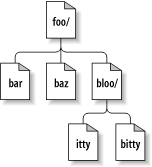
\includegraphics[keepaspectratio]{images/ch08dia1.png}}
\caption{Files and directories in two
dimensions}\label{svn.developer.layerlib.repos.dia-1}
\end{figure}

The difference here is that the Subversion filesystem has a nifty third
dimension that most filesystems do not have---Time!\footnote{We
  understand that this may come as a shock to sci-fi fans who have long
  been under the impression that Time was actually the \emph{fourth}
  dimension, and we apologize for any emotional trauma induced by our
  assertion of a different theory.} In the filesystem interface, nearly
every function that has a \texttt{path} argument also expects a
\texttt{root} argument. This \texttt{svn\_fs\_root\_t} argument
describes either a revision or a Subversion transaction (which is simply
a revision in the making) and provides that third dimension of context
needed to understand the difference between \texttt{/foo/bar} in
revision 32, and the same path as it exists in revision 98.
\hyperref[svn.developer.layerlib.repos.dia-2]{Versioning time---the
third dimension!} shows revision history as an added dimension to the
Subversion filesystem universe.

\begin{figure}
\centering
\pandocbounded{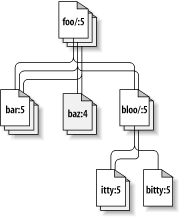
\includegraphics[keepaspectratio]{images/ch08dia2.png}}
\caption{Versioning time---the third
dimension!}\label{svn.developer.layerlib.repos.dia-2}
\end{figure}

As we mentioned earlier, the \texttt{libsvn\_fs} API looks and feels
like any other filesystem, except that it has this wonderful versioning
capability. It was designed to be usable by any program interested in a
versioning filesystem. Not coincidentally, Subversion itself is
interested in that functionality. But while the filesystem API should be
sufficient for basic file and directory versioning support, Subversion
wants more---and that is where \texttt{libsvn\_repos} comes in.

The Subversion repository library (\texttt{libsvn\_repos}) sits
(logically speaking) atop the \texttt{libsvn\_fs} API, providing
additional functionality beyond that of the underlying versioned
filesystem logic. It does not completely wrap each and every filesystem
function---only certain major steps in the general cycle of filesystem
activity are wrapped by the repository interface. Some of these include
the creation and commit of Subversion transactions and the modification
of revision properties. These particular events are wrapped by the
repository layer because they have hooks associated with them. A
repository hook system is not strictly related to implementing a
versioning filesystem, so it lives in the repository wrapper library.

The hooks mechanism is but one of the reasons for the abstraction of a
separate repository library from the rest of the filesystem code. The
\texttt{libsvn\_repos} API provides several other important utilities to
Subversion. These include the abilities to:

\begin{itemize}
\item
  Create, open, destroy, and perform recovery steps on a Subversion
  repository and the filesystem included in that repository.
\item
  Describe the differences between two filesystem trees.
\item
  Query for the commit log messages associated with all (or some) of the
  revisions in which a set of files was modified in the filesystem.
\item
  Generate a human-readable ``dump'' of the filesystem---a complete
  representation of the revisions in the filesystem.
\item
  Parse that dump format, loading the dumped revisions into a different
  Subversion repository.
\end{itemize}

As Subversion continues to evolve, the repository library will grow with
the filesystem library to offer increased functionality and configurable
option support.

\subsection{Repository Access Layer}\label{svn.developer.layerlib.ra}

If the Subversion Repository layer is at ``the other end of the line,''
the Repository Access (RA) layer is the line itself. Charged with
marshaling data between the client libraries and the repository, this
layer includes the \texttt{libsvn\_ra} module loader library, the RA
modules themselves (which currently includes \texttt{libsvn\_ra\_local},
\texttt{libsvn\_ra\_serf}, and \texttt{libsvn\_ra\_svn}), and any
additional libraries needed by one or more of those RA modules (such as
the \texttt{mod\_dav\_svn} Apache module or
\texttt{libsvn\_ra\_svn}\textquotesingle s server, \texttt{svnserve}).

Since Subversion uses URLs to identify its repository resources, the
protocol portion of the URL scheme (usually \texttt{file://},
\texttt{http://}, \texttt{https://}, \texttt{svn://}, or
\texttt{svn+ssh://}) is used to determine which RA module will handle
the communications. Each module registers a list of the protocols it
knows how to ``speak'' so that the RA loader can, at runtime, determine
which module to use for the task at hand. You can determine which RA
modules are available to the Subversion command-line client, and what
protocols they claim to support, by running \texttt{svn\ -\/-version}:

\begin{verbatim}
$ svn --version
svn, version 1.8.0-dev (under development)
   compiled Jan  8 2013, 11:45:25 on i686-pc-linux-gnu

Copyright (C) 2013 The Apache Software Foundation.
This software consists of contributions made by many people;
see the NOTICE file for more information.
Subversion is open source software, see http://subversion.apache.org/

The following repository access (RA) modules are available:

* ra_svn : Module for accessing a repository using the svn network protocol.
  - with Cyrus SASL authentication
  - handles 'svn' scheme
* ra_local : Module for accessing a repository on local disk.
  - handles 'file' scheme
* ra_serf : Module for accessing a repository via WebDAV protocol using serf.
  - handles 'http' scheme
  - handles 'https' scheme

$
\end{verbatim}

The public API exported by the RA layer contains functionality necessary
for sending and receiving versioned data to and from the repository. And
each of the available RA plug-ins is able to perform that task using a
specific protocol---\texttt{libsvn\_ra\_serf} speaks HTTP/WebDAV
(optionally using SSL encryption) with an Apache HTTP Server that is
running the \texttt{mod\_dav\_svn} Subversion server module;
\texttt{libsvn\_ra\_svn} speaks a custom network protocol with the
\texttt{svnserve} program; and so on.

For those who wish to access a Subversion repository using still another
protocol, that is precisely why the Repository Access layer is
modularized! Developers can simply write a new library that implements
the RA interface on one side and communicates with the repository on the
other. Your new library can use existing network protocols or you can
invent your own. You could use interprocess communication (IPC) calls,
or---let\textquotesingle s get crazy, shall we?---you could even
implement an email-based protocol. Subversion supplies the APIs; you
supply the creativity.

\subsection{Client Layer}\label{svn.developer.layerlib.client}

On the client side, the Subversion working copy is where all the action
takes place. The bulk of functionality implemented by the client-side
libraries exists for the sole purpose of managing working
copies---directories full of files and other subdirectories that serve
as a sort of local, editable ``reflection'' of one or more repository
locations---and propagating changes to and from the Repository Access
layer.

Subversion\textquotesingle s working copy library, \texttt{libsvn\_wc},
is directly responsible for managing the data in the working copies. To
accomplish this, the library stores administrative information about the
working copy within a special subdirectory. This subdirectory, named
\texttt{.svn}, is present in each working copy and contains various
other files and directories that record state and provide a private
workspace for administrative action. For those familiar with CVS, this
\texttt{.svn} subdirectory is similar in purpose to the \texttt{CVS}
administrative directories found in CVS working copies.

The Subversion client library, \texttt{libsvn\_client}, has the broadest
responsibility; its job is to mingle the functionality of the working
copy library with that of the Repository Access layer, and then to
provide the highest-level API to any application that wishes to perform
general revision control actions. For example, the function
\texttt{svn\_client\_checkout()} takes a URL as an argument. It passes
this URL to the RA layer and opens an authenticated session with a
particular repository. It then asks the repository for a certain tree,
and sends this tree into the working copy library, which then writes a
full working copy to disk (\texttt{.svn} directories and all).

The client library is designed to be used by any application. While the
Subversion source code includes a standard command-line client, it
should be very easy to write any number of GUI clients on top of the
client library. New GUIs (or any new client, really) for Subversion need
not be clunky wrappers around the included command-line client---they
have full access via the \texttt{libsvn\_client} API to the same
functionality, data, and callback mechanisms that the command-line
client uses. In fact, the Subversion source code tree contains a small C
program (which you can find at
\texttt{tools/examples/minimal\_client.c}) that exemplifies how to wield
the Subversion API to create a simple client program.

Binding Directly---A Word About Correctness

Why should your GUI program bind directly with a \texttt{libsvn\_client}
instead of acting as a wrapper around a command-line program? Besides
simply being more efficient, it can be more correct as well. A
command-line program (such as the one supplied with Subversion) that
binds to the client library needs to effectively translate feedback and
requested data bits from C types to some form of human-readable output.
This type of translation can be lossy. That is, the program may not
display all of the information harvested from the API or may combine
bits of information for compact representation.

If you wrap such a command-line program with yet another program, the
second program has access only to already interpreted (and as we
mentioned, likely incomplete) information, which it must \emph{again}
translate into \emph{its} representation format. With each layer of
wrapping, the integrity of the original data is potentially tainted more
and more, much like the result of making a copy of a copy (of a
copy\ldots) of a favorite audio or video cassette.

But the most compelling argument for binding directly to the APIs
instead of wrapping other programs is that the Subversion project makes
compatibility promises regarding its APIs. Across minor versions of
those APIs (such as between 1.3 and 1.4), no function\textquotesingle s
prototype will change. In other words, you aren\textquotesingle t forced
to update your program\textquotesingle s source code simply because
you\textquotesingle ve upgraded to a new version of Subversion. Certain
functions might be deprecated, but they still work, and this gives you a
buffer of time to eventually embrace the newer APIs. These kinds of
compatibility promises do not exist for Subversion command-line program
output, which is subject to change from release to release.

\section{Using the APIs}\label{svn.developer.usingapi}

Developing applications against the Subversion library APIs is fairly
straightforward. Subversion is primarily a set of C libraries, with
header (\texttt{.h}) files that live in the \texttt{subversion/include}
directory of the source tree. These headers are copied into your system
locations (e.g., \texttt{/usr/local/include}) when you build and install
Subversion itself from source. These headers represent the entirety of
the functions and types meant to be accessible by users of the
Subversion libraries. The Subversion developer community is meticulous
about ensuring that the public API is well documented---refer directly
to the header files for that documentation.

When examining the public header files, the first thing you might notice
is that Subversion\textquotesingle s datatypes and functions are
namespace-protected. That is, every public Subversion symbol name begins
with \texttt{svn\_}, followed by a short code for the library in which
the symbol is defined (such as \texttt{wc}, \texttt{client},
\texttt{fs}, etc.), followed by a single underscore (\texttt{\_}), and
then the rest of the symbol name. Semipublic functions (used among
source files of a given library but not by code outside that library,
and found inside the library directories themselves) differ from this
naming scheme in that instead of a single underscore after the library
code, they use a double underscore (\texttt{\_\ \_}). Functions that are
private to a given source file have no special prefixing and are
declared \texttt{static}. Of course, a compiler isn\textquotesingle t
interested in these naming conventions, but they help to clarify the
scope of a given function or datatype.

Another good source of information about programming against the
Subversion APIs is the project\textquotesingle s own hacking guidelines,
which you can find at
\href{https://subversion.apache.org/docs/community-guide/}{}. This
document contains useful information, which, while aimed at developers
and would-be developers of Subversion itself, is equally applicable to
folks developing against Subversion as a set of third-party
libraries.\footnote{After all, Subversion uses
  Subversion\textquotesingle s APIs, too.}

\subsection{The Apache Portable Runtime
Library}\label{svn.developer.usingapi.apr}

Along with Subversion\textquotesingle s own datatypes, you will see many
references to datatypes that begin with \texttt{apr\_}---symbols from
the Apache Portable Runtime (APR) library. APR is
Apache\textquotesingle s portability library, originally carved out of
its server code as an attempt to separate the OS-specific bits from the
OS-independent portions of the code. The result was a library that
provides a generic API for performing operations that differ mildly---or
wildly---from OS to OS. While the Apache HTTP Server was obviously the
first user of the APR library, the Subversion developers immediately
recognized the value of using APR as well. This means that there is
practically no OS-specific code in Subversion itself. Also, it means
that the Subversion client compiles and runs anywhere that the Apache
HTTP Server does. Currently, this list includes all flavors of Unix,
Win32, BeOS, OS/2, and Mac OS X.

In addition to providing consistent implementations of system calls that
differ across operating systems,\footnote{Subversion uses ANSI system
  calls and datatypes as much as possible.} APR gives Subversion
immediate access to many custom datatypes, such as dynamic arrays and
hash tables. Subversion uses these types extensively. But perhaps the
most pervasive APR datatype, found in nearly every Subversion API
prototype, is the \texttt{apr\_pool\_t}---the APR memory pool.
Subversion uses pools internally for all its memory allocation needs
(unless an external library requires a different memory management
mechanism for data passed through its API),\footnote{Berkeley DB is an
  example of such a library.} and while a person coding against the
Subversion APIs is not required to do the same, she \emph{is} required
to provide pools to the API functions that need them. This means that
users of the Subversion API must also link against APR, must call
\texttt{apr\_initialize()} to initialize the APR subsystem, and then
must create and manage pools for use with Subversion API calls,
typically by using \texttt{svn\_pool\_create()},
\texttt{svn\_pool\_clear()}, and \texttt{svn\_pool\_destroy()}.

Programming with Memory Pools

Almost every developer who has used the C programming language has at
some point sighed at the daunting task of managing memory usage.
Allocating enough memory to use, keeping track of those allocations,
freeing the memory when you no longer need it---these tasks can be quite
complex. And of course, failure to do those things properly can result
in a program that crashes itself, or worse, crashes the computer.

Higher-level languages, on the other hand, either take the job of memory
management away from you completely or make it something you toy with
only when doing extremely tight program optimization. Languages such as
Java and Python use garbage collection, allocating memory for objects
when needed, and automatically freeing that memory when the object is no
longer in use.

APR provides a middle-ground approach called pool-based memory
management. It allows the developer to control memory usage at a lower
resolution---per chunk (or ``pool'') of memory, instead of per allocated
object. Rather than using \texttt{malloc()} and friends to allocate
enough memory for a given object, you ask APR to allocate the memory
from a memory pool. When you\textquotesingle re finished using the
objects you\textquotesingle ve created in the pool, you destroy the
entire pool, effectively de-allocating the memory consumed by \emph{all}
the objects you allocated from it. Thus, rather than keeping track of
individual objects that need to be de-allocated, your program simply
considers the general lifetimes of those objects and allocates the
objects in a pool whose lifetime (the time between the
pool\textquotesingle s creation and its deletion) matches the
object\textquotesingle s needs.

\subsection{Functions and
Batons}\label{svn.developer.usingapi.funcsbatons}

To facilitate ``streamy'' (asynchronous) behavior and provide consumers
of the Subversion C API with hooks for handling information in
customizable ways, many functions in the API accept pairs of parameters:
a pointer to a callback function, and a pointer to a blob of memory
called a baton that carries context information for that callback
function. Batons are typically C structures with additional information
that the callback function needs but which is not given directly to the
callback function by the driving API function.

\subsection{URL and Path
Requirements}\label{svn.developer.usingapi.urlpath}

With remote version control operation as the whole point of
Subversion\textquotesingle s existence, it makes sense that some
attention has been paid to internationalization (i18n) support. After
all, while ``remote'' might mean ``across the office,'' it could just as
well mean ``across the globe.'' To facilitate this, all of
Subversion\textquotesingle s public interfaces that accept path
arguments expect those paths to be canonicalized---which is most easily
accomplished by passing them through
\texttt{svn\_dirent\_canonicalize()} or
\texttt{svn\_uri\_canonicalize()} (depending on whether you are
canonicalizing a local system path or a URL, respectively)---and encoded
in UTF-8. This means, for example, that any new client binary that
drives the \texttt{libsvn\_client} interface needs to first convert
paths from the locale-specific encoding to UTF-8 before passing those
paths to the Subversion libraries, and then reconvert any resultant
output paths from Subversion back into the locale\textquotesingle s
encoding before using those paths for non-Subversion purposes.
Fortunately, Subversion provides a suite of functions (see
\texttt{subversion/include/svn\_utf.h}) that any program can use to do
these conversions.

Also, Subversion APIs require all URL parameters to be properly
URI-encoded. So, instead of passing
\url{file:///home/username/My\%C2\%A0File.txt} as the URL of a file
named \texttt{My\ File.txt}, you need to pass
\url{file:///home/username/My\%20File.txt}. Again, Subversion supplies
helper functions that your application can
use---\texttt{svn\_path\_uri\_encode()} and
\texttt{svn\_path\_uri\_decode()}, for URI encoding and decoding,
respectively.

\subsection{Using Languages Other Than C and
C++}\label{svn.developer.usingapi.otherlangs}

If you are interested in using the Subversion libraries in conjunction
with something other than a C program---say, a Python or Perl
script---Subversion has some support for this via the Simplified Wrapper
and Interface Generator (SWIG). The SWIG bindings for Subversion are
located in \texttt{subversion/bindings/swig}. They are still maturing,
but they are usable. These bindings allow you to call Subversion API
functions indirectly, using wrappers that translate the datatypes native
to your scripting language into the datatypes needed by
Subversion\textquotesingle s C libraries.

Significant efforts have been made toward creating functional
SWIG-generated bindings for Python, Perl, and Ruby. To some extent, the
work done preparing the SWIG interface files for these languages is
reusable in efforts to generate bindings for other languages supported
by SWIG (which include versions of C\#, Guile, Java, MzScheme, OCaml,
PHP, and Tcl, among others). However, some extra programming is required
to compensate for complex APIs that SWIG needs some help translating
between languages. For more information on SWIG itself, see the
project\textquotesingle s web site at \href{https://www.swig.org/}{}.

Subversion also has language bindings for Java. The javahl bindings
(located in \texttt{subversion/bindings/java} in the Subversion source
tree) aren\textquotesingle t SWIG-based, but are instead a mixture of
Java and hand-coded JNI. Javahl covers most Subversion client-side APIs
and is specifically targeted at implementors of Java-based Subversion
clients and IDE integrations.

Subversion\textquotesingle s language bindings tend to lack the level of
developer attention given to the core Subversion modules, but can
generally be trusted as production-ready. A number of scripts and
applications, alternative Subversion GUI clients, and other third-party
tools are successfully using Subversion\textquotesingle s language
bindings today to accomplish their Subversion integrations.

It\textquotesingle s worth noting here that there are other options for
interfacing with Subversion using other languages: alternative bindings
for Subversion that aren\textquotesingle t provided by the Subversion
development community at all. There are a couple of popular ones we feel
are especially noteworthy. First, Barry Scott\textquotesingle s PySVN
bindings (\href{https://pysvn.sourceforge.io/}{}) are a popular option
for binding with Python. PySVN boasts of a more Pythonic interface than
the more C-like APIs provided by Subversion\textquotesingle s own Python
bindings. And if you\textquotesingle re looking for a pure Java
implementation of Subversion, check out SVNKit
(\href{https://svnkit.com/}{}), which is Subversion rewritten from the
ground up in Java.

SVNKit Versus javahl

In 2005, a small company called TMate announced the 1.0.0 release of
JavaSVN---a pure Java implementation of Subversion. Since then, the
project has been renamed to SVNKit (available at
\href{https://svnkit.com/}{}) and has seen great success as a provider
of Subversion functionality to various Subversion clients, IDE
integrations, and other third-party tools.

The SVNKit library is interesting in that, unlike the javahl library, it
is not merely a wrapper around the official Subversion core libraries.
In fact, it shares no code with Subversion at all. But while it is easy
to confuse SVNKit with javahl, and easier still to not even realize
which of these libraries you are using, folks should be aware that
SVNKit differs from javahl in some significant ways. First, while SVNKit
is developed as open source software just like Subversion,
SVNKit\textquotesingle s license is more restrictive than that of
Subversion.\footnote{Redistributions in any form must be accompanied by
  information on how to obtain complete source code for the software
  that uses SVNKit and any accompanying software that uses the software
  that uses SVNKit. See \href{https://svnkit.com/license.html}{} for
  details.} Finally, by aiming to be a pure Java Subversion library,
SVNKit is limited in which portions of Subversion can be reasonably
cloned while still keeping up with Subversion\textquotesingle s
releases. This has already happened once---SVNKit cannot access
BDB-backed Subversion repositories via the \texttt{file://} protocol
because there\textquotesingle s no pure Java implementation of Berkeley
DB that is file-format-compatible with the native implementation of that
library.

That said, SVNKit has a well-established track record of reliability.
And a pure Java solution is much more robust in the face of programming
errors---a bug in SVNKit might raise a catchable Java Exception, but a
bug in the Subversion core libraries as accessed via javahl can bring
down your entire Java Runtime Environment. So, weigh the costs when
choosing a Java-based Subversion implementation.

\subsection{Code Samples}\label{svn.developer.usingapi.codesamples}

\hyperref[svn.developer.layerlib.repos.ex-1]{Using the repository layer}
contains a code segment (written in C) that illustrates some of the
concepts we\textquotesingle ve been discussing. It uses both the
repository and filesystem interfaces (as can be determined by the
prefixes \texttt{svn\_repos\_} and \texttt{svn\_fs\_} of the function
names, respectively) to create a new revision in which a directory is
added. You can see the use of an APR pool, which is passed around for
memory allocation purposes. Also, the code reveals a somewhat obscure
fact about Subversion error handling---all Subversion errors must be
explicitly handled to avoid memory leakage (and in some cases,
application failure).

\protect\phantomsection\label{svn.developer.layerlib.repos.ex-1}
Using the repository layer

\begin{verbatim}
/* Convert a Subversion error into a simple boolean error code.
 *
 * NOTE:  Subversion errors must be cleared (using svn_error_clear())
 *        because they are allocated from the global pool, else memory
 *        leaking occurs.
 */
#define INT_ERR(expr)                           \
  do {                                          \
    svn_error_t *__temperr = (expr);            \
    if (__temperr)                              \
      {                                         \
        svn_error_clear(__temperr);             \
        return 1;                               \
      }                                         \
    return 0;                                   \
  } while (0)

/* Create a new directory at the path NEW_DIRECTORY in the Subversion
 * repository located at REPOS_PATH.  Perform all memory allocation in
 * POOL.  This function will create a new revision for the addition of
 * NEW_DIRECTORY.  Return zero if the operation completes
 * successfully, nonzero otherwise.
 */
static int
make_new_directory(const char *repos_path,
                   const char *new_directory,
                   apr_pool_t *pool)
{
  svn_error_t *err;
  svn_repos_t *repos;
  svn_fs_t *fs;
  svn_revnum_t youngest_rev;
  svn_fs_txn_t *txn;
  svn_fs_root_t *txn_root;
  const char *conflict_str;

  /* Open the repository located at REPOS_PATH. 
   */
  INT_ERR(svn_repos_open(&repos, repos_path, pool));

  /* Get a pointer to the filesystem object that is stored in REPOS. 
   */
  fs = svn_repos_fs(repos);

  /* Ask the filesystem to tell us the youngest revision that
   * currently exists. 
   */
  INT_ERR(svn_fs_youngest_rev(&youngest_rev, fs, pool));

  /* Begin a new transaction that is based on YOUNGEST_REV.  We are
   * less likely to have our later commit rejected as conflicting if we
   * always try to make our changes against a copy of the latest snapshot
   * of the filesystem tree. 
   */
  INT_ERR(svn_repos_fs_begin_txn_for_commit2(&txn, repos, youngest_rev,
                                             apr_hash_make(pool), pool));

  /* Now that we have started a new Subversion transaction, get a root
   * object that represents that transaction. 
   */
  INT_ERR(svn_fs_txn_root(&txn_root, txn, pool));
  
  /* Create our new directory under the transaction root, at the path
   * NEW_DIRECTORY. 
   */
  INT_ERR(svn_fs_make_dir(txn_root, new_directory, pool));

  /* Commit the transaction, creating a new revision of the filesystem
   * which includes our added directory path.
   */
  err = svn_repos_fs_commit_txn(&conflict_str, repos, 
                                &youngest_rev, txn, pool);
  if (! err)
    {
      /* No error?  Excellent!  Print a brief report of our success.
       */
      printf("Directory '%s' was successfully added as new revision "
             "'%ld'.\n", new_directory, youngest_rev);
    }
  else if (err->apr_err == SVN_ERR_FS_CONFLICT)
    {
      /* Uh-oh.  Our commit failed as the result of a conflict
       * (someone else seems to have made changes to the same area 
       * of the filesystem that we tried to modify).  Print an error
       * message.
       */
      printf("A conflict occurred at path '%s' while attempting "
             "to add directory '%s' to the repository at '%s'.\n", 
             conflict_str, new_directory, repos_path);
    }
  else
    {
      /* Some other error has occurred.  Print an error message.
       */
      printf("An error occurred while attempting to add directory '%s' "
             "to the repository at '%s'.\n", 
             new_directory, repos_path);
    }

  INT_ERR(err);
} 
\end{verbatim}

Note that in \hyperref[svn.developer.layerlib.repos.ex-1]{Using the
repository layer}, the code could just as easily have committed the
transaction using \texttt{svn\_fs\_commit\_txn()}. But the filesystem
API knows nothing about the repository library\textquotesingle s hook
mechanism. If you want your Subversion repository to automatically
perform some set of non-Subversion tasks every time you commit a
transaction (e.g., sending an email that describes all the changes made
in that transaction to your developer mailing list), you need to use the
\texttt{libsvn\_repos}-wrapped version of that function, which adds the
hook triggering functionality---in this case,
\texttt{svn\_repos\_fs\_commit\_txn()}. (For more information regarding
Subversion\textquotesingle s repository hooks, see
\hyperref[svn.reposadmin.hooks]{Implementing Repository Hooks}.)

Now let\textquotesingle s switch languages.
\hyperref[svn.developer.usingapi.otherlangs.ex-1]{Using the repository
layer with Python} is a sample program that uses
Subversion\textquotesingle s SWIG Python bindings to recursively crawl
the youngest repository revision, and to print the various paths reached
during the crawl.

\protect\phantomsection\label{svn.developer.usingapi.otherlangs.ex-1}
Using the repository layer with Python

\begin{verbatim}
#!/usr/bin/python

"""Crawl a repository, printing versioned object path names."""

import sys
import os.path
import svn.fs, svn.core, svn.repos

def crawl_filesystem_dir(root, directory):
    """Recursively crawl DIRECTORY under ROOT in the filesystem, and return
    a list of all the paths at or below DIRECTORY."""

    # Print the name of this path.
    print directory + "/"
    
    # Get the directory entries for DIRECTORY.
    entries = svn.fs.svn_fs_dir_entries(root, directory)

    # Loop over the entries.
    names = entries.keys()
    for name in names:
        # Calculate the entry's full path.
        full_path = directory + '/' + name

        # If the entry is a directory, recurse.  The recursion will return
        # a list with the entry and all its children, which we will add to
        # our running list of paths.
        if svn.fs.svn_fs_is_dir(root, full_path):
            crawl_filesystem_dir(root, full_path)
        else:
            # Else it's a file, so print its path here.
            print full_path

def crawl_youngest(repos_path):
    """Open the repository at REPOS_PATH, and recursively crawl its
    youngest revision."""
    
    # Open the repository at REPOS_PATH, and get a reference to its
    # versioning filesystem.
    repos_obj = svn.repos.svn_repos_open(repos_path)
    fs_obj = svn.repos.svn_repos_fs(repos_obj)

    # Query the current youngest revision.
    youngest_rev = svn.fs.svn_fs_youngest_rev(fs_obj)
    
    # Open a root object representing the youngest (HEAD) revision.
    root_obj = svn.fs.svn_fs_revision_root(fs_obj, youngest_rev)

    # Do the recursive crawl.
    crawl_filesystem_dir(root_obj, "")
    
if __name__ == "__main__":
    # Check for sane usage.
    if len(sys.argv) != 2:
        sys.stderr.write("Usage: %s REPOS_PATH\n"
                         % (os.path.basename(sys.argv[0])))
        sys.exit(1)

    # Canonicalize the repository path.
    repos_path = svn.core.svn_dirent_canonicalize(sys.argv[1])

    # Do the real work.
    crawl_youngest(repos_path)
\end{verbatim}

This same program in C would need to deal with APR\textquotesingle s
memory pool system. But Python handles memory usage automatically, and
Subversion\textquotesingle s Python bindings adhere to that convention.
In C, you\textquotesingle d be working with custom datatypes (such as
those provided by the APR library) for representing the hash of entries
and the list of paths, but Python has hashes (called ``dictionaries'')
and lists as built-in datatypes, and it provides a rich collection of
functions for operating on those types. So SWIG (with the help of some
customizations in Subversion\textquotesingle s language bindings layer)
takes care of mapping those custom datatypes into the native datatypes
of the target language. This provides a more intuitive interface for
users of that language.

The Subversion Python bindings can be used for working copy operations,
too. In the previous section of this chapter, we mentioned the
\texttt{libsvn\_client} interface and how it exists for the sole purpose
of simplifying the process of writing a Subversion client.
\hyperref[svn.developer.usingapi.otherlangs.ex-2]{A Python status
crawler} is a brief example of how that library can be accessed via the
SWIG Python bindings to re-create a scaled-down version of the
\texttt{svn\ status} command.

\protect\phantomsection\label{svn.developer.usingapi.otherlangs.ex-2}
A Python status crawler

\begin{verbatim}
#!/usr/bin/env python

"""Crawl a working copy directory, printing status information."""

import sys
import os.path
import getopt
import svn.core, svn.client, svn.wc

def generate_status_code(status):
    """Translate a status value into a single-character status code,
    using the same logic as the Subversion command-line client."""
    code_map = { svn.wc.svn_wc_status_none        : ' ',
                 svn.wc.svn_wc_status_normal      : ' ',
                 svn.wc.svn_wc_status_added       : 'A',
                 svn.wc.svn_wc_status_missing     : '!',
                 svn.wc.svn_wc_status_incomplete  : '!',
                 svn.wc.svn_wc_status_deleted     : 'D',
                 svn.wc.svn_wc_status_replaced    : 'R',
                 svn.wc.svn_wc_status_modified    : 'M',
                 svn.wc.svn_wc_status_conflicted  : 'C',
                 svn.wc.svn_wc_status_obstructed  : '~',
                 svn.wc.svn_wc_status_ignored     : 'I',
                 svn.wc.svn_wc_status_external    : 'X',
                 svn.wc.svn_wc_status_unversioned : '?',
               }
    return code_map.get(status, '?')

def do_status(wc_path, verbose, prefix):
    # Build a client context baton.
    ctx = svn.client.svn_client_create_context()

    def _status_callback(path, status):
        """A callback function for svn_client_status."""

        # Print the path, minus the bit that overlaps with the root of
        # the status crawl
        text_status = generate_status_code(status.text_status)
        prop_status = generate_status_code(status.prop_status)
        prefix_text = ''
        if prefix is not None:
            prefix_text = prefix + " "
        print '%s%s%s  %s' % (prefix_text, text_status, prop_status, path)
        
    # Do the status crawl, using _status_callback() as our callback function.
    revision = svn.core.svn_opt_revision_t()
    revision.type = svn.core.svn_opt_revision_head
    svn.client.svn_client_status2(wc_path, revision, _status_callback,
                                  svn.core.svn_depth_infinity, verbose,
                                  0, 0, 1, ctx)

def usage_and_exit(errorcode):
    """Print usage message, and exit with ERRORCODE."""
    stream = errorcode and sys.stderr or sys.stdout
    stream.write("""Usage: %s OPTIONS WC-PATH

  Print working copy status, optionally with a bit of prefix text.

Options:
  --help, -h    : Show this usage message
  --prefix ARG  : Print ARG, followed by a space, before each line of output
  --verbose, -v : Show all statuses, even uninteresting ones
""" % (os.path.basename(sys.argv[0])))
    sys.exit(errorcode)
    
if __name__ == '__main__':
    # Parse command-line options.
    try:
        opts, args = getopt.getopt(sys.argv[1:], "hv",
                                   ["help", "prefix=", "verbose"])
    except getopt.GetoptError:
        usage_and_exit(1)
    verbose = 0
    prefix = None
    for opt, arg in opts:
        if opt in ("-h", "--help"):
            usage_and_exit(0)
        if opt in ("--prefix"):
            prefix = arg
        if opt in ("-v", "--verbose"):
            verbose = 1
    if len(args) != 1:
        usage_and_exit(2)
            
    # Canonicalize the working copy path.
    wc_path = svn.core.svn_dirent_canonicalize(args[0])

    # Do the real work.
    try:
        do_status(wc_path, verbose, prefix)
    except svn.core.SubversionException, e:
        sys.stderr.write("Error (%d): %s\n" % (e.apr_err, e.message))
        sys.exit(1)
\end{verbatim}

As was the case in
\hyperref[svn.developer.usingapi.otherlangs.ex-1]{Using the repository
layer with Python}, this program is pool-free and uses, for the most
part, normal Python datatypes.

Run user-provided paths through the appropriate canonicalization
function (\texttt{svn\_dirent\_canonicalize()} or
\texttt{svn\_uri\_canonicalize()}) before passing them to other API
functions. Failure to do so can trigger assertions in the underlying
Subversion C library which translate into rather immediate and
unceremonious program abortion.

Of particular interest to users of the Python flavor of
Subversion\textquotesingle s API is the implementation of callback
functions. As previously mentioned, Subversion\textquotesingle s C API
makes liberal use of the callback function/baton paradigm. API functions
which in C accept a function and baton pair only accept a callback
function parameter in Python. How, then, does the caller pass arbitrary
context information to the callback function? In Python, this is done by
taking advantage of Python\textquotesingle s scoping rules and default
argument values. You can see this in action in
\hyperref[svn.developer.usingapi.otherlangs.ex-2]{A Python status
crawler}. The \texttt{svn\_client\_status2()} function is given a
callback function (\texttt{\_status\_callback()}) but no
baton---\texttt{\_status\_callback()} gets access to the user-provided
prefix string because that variable falls into the scope of the function
automatically.

\section{Summary}\label{svn.developer.summary}

One of Subversion\textquotesingle s greatest features
isn\textquotesingle t something you get from running its command-line
client or other tools. It\textquotesingle s the fact that Subversion was
designed modularly and provides a stable, public API so that
others---like yourself, perhaps---can write custom software that drives
Subversion\textquotesingle s core logic.

In this chapter, we took a closer look at Subversion\textquotesingle s
architecture, examining its logical layers and describing that public
API, the very same API that Subversion\textquotesingle s own layers use
to communicate with each other. Many developers have found interesting
uses for the Subversion API, from simple repository hook scripts, to
integrations between Subversion and some other application, to
completely different version control systems. What unique itch will
\emph{you} scratch with it?


\part{Subversion Command Reference}\label{svn.ref}

\chapter{svn Reference---Subversion Command-Line
Client}\label{svn.ref.svn}

\texttt{svn} is the official command-line client of Subversion. Its
functionality is offered via a collection of task-specific subcommands,
most of which accept a number of options for fine-grained control of the
program\textquotesingle s behavior.

When using the \texttt{svn} program, subcommands and other non-option
arguments must appear in a specified order on the command line. Options,
on the other hand, may appear anywhere on the command line (after the
program name, of course), and in general, their order is irrelevant. For
example, all of the following are valid ways to use
\texttt{svn\ status}, and are interpreted in exactly the same way:

\begin{verbatim}
$ svn -vq status myfile
$ svn status -v -q myfile
$ svn -q status -v myfile
$ svn status -vq myfile
$ svn status myfile -qv
\end{verbatim}

The following sections describe each of the various subcommands and
options provided by the \texttt{svn} command-line client program,
including some examples of each subcommand\textquotesingle s typical
uses.

While Subversion has different options for its subcommands, all options
exist in a single namespace---that is, each option is guaranteed to mean
the roughly same thing regardless of the subcommand you use it with. For
example, \texttt{-\/-verbose} (\texttt{-v}) always means ``verbose
output,'' regardless of the subcommand you use it with.

The \texttt{svn} command-line client usually exits quickly with an error
if you pass it an option which does not apply to the specified
subcommand. But as of Subversion 1.5, several of the options which apply
to all---or nearly all---of the subcommands have been deemed acceptable
by all subcommands, even if they have no effect on some of them. (This
change was made primarily to improve the client\textquotesingle s
ability to called from custom wrapping scripts.) These options appear
grouped together in the command-line client\textquotesingle s usage
messages as global options, as can be seen in the following bit of
output:

\begin{verbatim}
$ svn help upgrade
upgrade: Upgrade the metadata storage format for a working copy.
usage: upgrade [WCPATH...]

  Local modifications are preserved.

Valid options:
  -q [--quiet]             : print nothing, or only summary information

Global options:
  --username ARG           : specify a username ARG
  --password ARG           : specify a password ARG
  --no-auth-cache          : do not cache authentication tokens
  --non-interactive        : do no interactive prompting (default is to prompt
                             only if standard input is a terminal device)
  --force-interactive      : do interactive prompting even if standard input
                             is not a terminal device
  --trust-server-cert      : accept SSL server certificates from unknown
                             certificate authorities without prompting (but only
                             with '--non-interactive')
  --config-dir ARG         : read user configuration files from directory ARG
  --config-option ARG      : set user configuration option in the format:
                                 FILE:SECTION:OPTION=[VALUE]
                             For example:
                                 servers:global:http-library=serf
$
\end{verbatim}

\texttt{svn} subcommands recognize the following options:

\protect\phantomsection\label{svn.ref.svn.sw}{}

\begin{description}
\item[\protect\phantomsection\label{svn.ref.svn.sw.accept}{}\texttt{-\/-accept}
\textless ACTION\textgreater{}]
Specifies an action for automatic conflict resolution, disabling the
interactive prompts which ask the user how to handle each conflict as it
is noticed. Though which of the specific actions are applicable differs
depending on which subcommand is in use, Subversion supports the
following long (and short) values for \textless ACTION\textgreater:

\begin{description}
\item[\texttt{postpone} (\texttt{p})]
Take no resolution action at all and instead allow the conflicts to be
recorded for future resolution.
\item[\texttt{edit} (\texttt{e})]
Open each conflicted file in a text editor for manual resolution of
line-based conflicts.
\item[\texttt{launch} (\texttt{l})]
Launch an interactive merge conflict resolution tool for each conflicted
file.
\item[\texttt{base}]
Choose the file that was the (unmodified) \texttt{BASE} revision before
you tried to integrate changes from the server into your working copy.
\item[\texttt{working}]
Assuming that you\textquotesingle ve manually handled the conflict
resolution, choose the version of the file as it currently stands in
your working copy.
\item[\texttt{mine-full} (\texttt{mf})]
Resolve conflicted files by preserving all local modifications and
discarding all changes fetched from the server during the operation
which caused the conflict.
\item[\texttt{theirs-full} (\texttt{tf})]
Resolve conflicted files by discarding all local modifications and
integrating all changes fetched from the server during the operation
which caused the conflict.
\item[\texttt{mine-conflict} (\texttt{mc})]
Resolve conflicted files by preferring local modifications over the
changes fetched from the server in conflicting regions of each
file\textquotesingle s content.
\item[\texttt{theirs-conflict} (\texttt{tc})]
Resolve conflicted files by preferring the changes fetched from the
server over local modifications in conflicting regions of each
file\textquotesingle s content.
\end{description}

Consult the output of \texttt{svn\ help\ SUBCOMMAND} to see exactly
which actions are supported by the specific subcommand of interest.
\item[\protect\phantomsection\label{svn.ref.svn.sw.allow_mixed_revisions}{}\texttt{-\/-allow-mixed-revisions}]
Disables the verification---performed by default by \texttt{svn\ merge}
as of Subversion 1.7---that the target of a merge operation and all of
its children are at a uniform revision. While merging into a
single-revision working copy target is the recommended best practice,
this option may be used to permit merges into mixed-revision working
copies as necessary.
\item[\protect\phantomsection\label{svn.ref.svn.sw.auto_props}{}\texttt{-\/-auto-props}]
Enables automatic property assignment (per runtime configuration rules),
overriding the \texttt{enable-auto-props} runtime configuration
directive.
\item[\protect\phantomsection\label{svn.ref.svn.sw.change}{}\texttt{-\/-change}
(\texttt{-c}) \textless ARG\textgreater{}]
Perform the requested operation using a specific ``change''. Generally
speaking, this option is syntactic sugar for \texttt{-r\ ARG-1:ARG}.
Some subcommands permit a comma-separated list of revision number
arguments (e.g., \texttt{-c\ ARG1,ARG2,ARG3}). Alternatively, you can
provide two arguments separated by a dash (as in \texttt{-c\ ARG1-ARG2})
to identify the range of revisions between \textless ARG1\textgreater{}
and \textless ARG2\textgreater, inclusive. Finally, if the revision
argument is negated, the implied revision range is reversed:
\texttt{-c\ -45} is equivalent to \texttt{-r\ 45:44}.
\item[\protect\phantomsection\label{svn.ref.svn.sw.changelist}{}\texttt{-\/-changelist}
(\texttt{-\/-cl}) \textless ARG\textgreater{}]
Instructs Subversion to operate only on members of the changelist named
\textless ARG\textgreater. You can use this option multiple times to
specify sets of changelists.
\item[\protect\phantomsection\label{svn.ref.svn.sw.config_dir}{}\texttt{-\/-config-dir}
\textless DIR\textgreater{}]
Instructs Subversion to read configuration information from the
specified directory instead of the default location
(\texttt{.subversion} in the user\textquotesingle s home directory).

This option is accepted by all \texttt{svn} subcommands.
\item[\protect\phantomsection\label{svn.ref.svn.sw.config_option}{}\texttt{-\/-config-option}
\textless CONFSPEC\textgreater{}]
Sets, for the duration of the command, the value of a runtime
configuration option. \textless CONFSPEC\textgreater{} is a string which
specifies the configuration option namespace, name and value that
you\textquotesingle d like to assign, formatted as
\textless FILE\textgreater:\textless SECTION\textgreater:\textless OPTION\textgreater={[}\textless VALUE\textgreater{]}.
In this syntax, \textless FILE\textgreater{} and
\textless SECTION\textgreater{} are the runtime configuration file
(either \texttt{config} or \texttt{servers}) and the section thereof,
respectively, which contain the option whose value you wish to change.
\textless OPTION\textgreater{} is, of course, the option itself, and
\textless VALUE\textgreater{} the value (if any) you wish to assign to
the option. For example, to temporarily disable the use of the
compression in the HTTP protocol, use
\texttt{-\/-config-option=servers:global:http-compression=no}. You can
use this option multiple times to change multiple option values
simultaneously.

This option is accepted by all \texttt{svn} subcommands.
\item[\protect\phantomsection\label{svn.ref.svn.sw.depth}{}\texttt{-\/-depth}
\textless ARG\textgreater{}]
Instructs Subversion to limit the scope of an operation to a particular
tree depth. \textless ARG\textgreater{} is one of \texttt{empty} (only
the target itself), \texttt{files} (the target and any immediate file
children thereof), \texttt{immediates} (the target and any immediate
children thereof), or \texttt{infinity} (the target and all of its
descendants---full recursion).
\item[\protect\phantomsection\label{svn.ref.svn.sw.diff}{}\texttt{-\/-diff}]
Enables a special output mode for \texttt{svn\ log} which includes a
difference report (a la \texttt{svn\ diff}) as part of each
revision\textquotesingle s information.
\item[\protect\phantomsection\label{svn.ref.svn.sw.diff_cmd}{}\texttt{-\/-diff-cmd}
\textless CMD\textgreater{}]
Specifies an external program to use to show differences between files.
When \texttt{svn\ diff} is invoked without this option, it uses
Subversion\textquotesingle s internal differencing engine, which
provides unified diffs by default. If you want to use an external
differencing program, use \texttt{-\/-diff-cmd}. You can then pass
options to the specified program using the \texttt{-\/-extensions}
(\texttt{-x}) option.
\item[\protect\phantomsection\label{svn.ref.svn.sw.diff3_cmd}{}\texttt{-\/-diff3-cmd}
\textless CMD\textgreater{}]
Specifies an external 3-way differencing program (used to merge
line-based changes into files).
\item[\protect\phantomsection\label{svn.ref.svn.sw.dry_run}{}\texttt{-\/-dry-run}]
Goes through all the motions of running a command, but makes no actual
changes---either on disk or in the repository.
\item[\protect\phantomsection\label{svn.ref.svn.sw.editor_cmd}{}\texttt{-\/-editor-cmd}
\textless CMD\textgreater{}]
Specifies an external program to use to edit a log message or a property
value. See the \texttt{editor-cmd} section in
\hyperref[svn.advanced.confarea.opts.config]{General configuration} for
ways to specify a default editor.
\item[\protect\phantomsection\label{svn.ref.svn.sw.encoding}{}\texttt{-\/-encoding}
\textless ENC\textgreater{}]
Tells Subversion that your commit message is composed using the
character encoding provided. The default character encoding is derived
from your operating system\textquotesingle s native locale; use this
option if your commit message is composed using any other encoding.
\item[\protect\phantomsection\label{svn.ref.svn.sw.extensions}{}\texttt{-\/-extensions}
(\texttt{-x}) \textless ARG\textgreater{}]
Specifies customizations which Subversion should make when performing
difference calculations. Valid extensions include:

\begin{description}
\item[\texttt{-\/-ignore-space-change} (\texttt{-b})]
Ignore changes in the amount of white space.
\item[\texttt{-\/-ignore-all-space} (\texttt{-w})]
Ignore all white space.
\item[\texttt{-\/-ignore-eol-style}]
Ignore changes in EOL (end-of-line) style.
\item[\texttt{-\/-show-c-function} (\texttt{-p})]
Show C function names in the diff output.
\item[\texttt{-\/-unified} (\texttt{-u})]
Show three lines of unified diff context.
\end{description}

The default value of \textless ARG\textgreater{} is \texttt{-u}. If you
wish to pass multiple arguments, you must enclose all of them in quotes.

Note that when Subversion is configured to invoke an external diff
command, the value of the \texttt{-\/-extensions} (\texttt{-x}) option
isn\textquotesingle t restricted to the previously mentioned options,
but may be \emph{any} additional arguments which Subversion should pass
to that command.
\item[\protect\phantomsection\label{svn.ref.svn.sw.file}{}\texttt{-\/-file}
(\texttt{-F}) \textless FILENAME\textgreater{}]
Uses the contents of the named file for the specified subcommand.
Different subcommands do different things with this content. For
example, \texttt{svn\ commit} uses the content as a commit log message,
whereas \texttt{svn\ propset} uses it as a property value.
\item[\protect\phantomsection\label{svn.ref.svn.sw.force}{}\texttt{-\/-force}]
Forces a particular command or operation to run. Subversion will prevent
you from performing some operations in normal usage, but you can pass
this option to tell Subversion ``I know what I\textquotesingle m doing
as well as the possible repercussions of doing it, so let me at
\textquotesingle em.'' This option is the programmatic equivalent of
doing your own electrical work with the power on---if you
don\textquotesingle t know what you\textquotesingle re doing,
you\textquotesingle re likely to get a nasty shock.
\item[\protect\phantomsection\label{svn.ref.svn.sw.force_log}{}\texttt{-\/-force-log}]
Forces a suspicious parameter passed to the \texttt{-\/-message}
(\texttt{-m}) or \texttt{-\/-file} (\texttt{-F}) option to be accepted
as valid. By default, Subversion will produce an error if parameters to
these options look like they might instead be targets of the subcommand.
For example, if you pass a versioned file\textquotesingle s path to the
\texttt{-\/-file} (\texttt{-F}) option, Subversion will assume
you\textquotesingle ve made a mistake, that the path was instead
intended as the target of the operation, and that you simply failed to
provide some other---unversioned---file as the source of your log
message. To assert your intent and override these types of errors, pass
the \texttt{-\/-force-log} option to subcommands that accept log
messages.
\item[\protect\phantomsection\label{svn.ref.svn.sw.force_interactive}{}\texttt{-\/-force-interactive}]
Forces the \texttt{svn} command-line client to run in interactive mode
when standard input is not a terminal device.

This option is accepted by all \texttt{svn} subcommands.
\item[\protect\phantomsection\label{svn.ref.svn.sw.git}{}\texttt{-\/-git}]
Enables a special output mode for \texttt{svn\ diff} designed for
cross-compatibility with the popular Git distributed version control
system.
\item[\protect\phantomsection\label{svn.ref.svn.sw.help}{}\texttt{-\/-help}
(\texttt{-h}, \texttt{-?})]
If used with one or more subcommands, shows the built-in help text for
each. If used alone, it displays the general client help text.
\item[\protect\phantomsection\label{svn.ref.svn.sw.ignore_ancestry}{}\texttt{-\/-ignore-ancestry}]
Tells Subversion to ignore ancestry when calculating differences (rely
on path contents alone). Also disables
\hyperref[svn.branchmerge.basicmerging.mergetracking]{Merge Tracking}
when used with the \texttt{svn\ merge} subcommand.
\item[\protect\phantomsection\label{svn.ref.svn.sw.ignore_externals}{}\texttt{-\/-ignore-externals}]
Tells Subversion to ignore externals definitions and the external
working copies managed by them.
\item[\protect\phantomsection\label{svn.ref.svn.sw.ignore_keywords}{}\texttt{-\/-ignore-keywords}]
Disables keyword expansion.
\item[\protect\phantomsection\label{svn.ref.svn.sw.ignore_properties}{}\texttt{-\/-ignore-properties}]
Instructs \texttt{svn\ diff} to suppress output of property changes.
\item[\protect\phantomsection\label{svn.ref.svn.sw.ignore_whitespace}{}\texttt{-\/-ignore-whitespace}]
Instructs \texttt{svn\ patch} to ignore whitespace when attempting to
identify patch context.
\item[\protect\phantomsection\label{svn.ref.svn.sw.incremental}{}\texttt{-\/-incremental}]
Prints output in a format suitable for concatenation to prior similar
output.
\item[\protect\phantomsection\label{svn.ref.svn.sw.internal_diff}{}\texttt{-\/-internal-diff}]
Instructs Subversion to use its built-in differencing engine despite any
external differencing mechanism that may be specified for use in the
user\textquotesingle s runtime configuration.
\item[\protect\phantomsection\label{svn.ref.svn.sw.keep_changelists}{}\texttt{-\/-keep-changelists}]
Tells Subversion not to remove the changelist assigments from working
copy items after committing.
\item[\protect\phantomsection\label{svn.ref.svn.sw.keep_local}{}\texttt{-\/-keep-local}]
Keeps the local copy of a file or directory (used with the
\texttt{svn\ delete} command).
\item[\protect\phantomsection\label{svn.ref.svn.sw.limit}{}\texttt{-\/-limit}
(\texttt{-l}) \textless NUM\textgreater{}]
Shows only the first \textless NUM\textgreater{} log messages.
\item[\protect\phantomsection\label{svn.ref.svn.sw.message}{}\texttt{-\/-message}
(\texttt{-m}) \textless MESSAGE\textgreater{}]
Indicates that you will specify either a log message or a lock comment
on the command line, following this option. For example:

\begin{verbatim}
$ svn commit -m "They don't make Sunday."
\end{verbatim}
\item[\protect\phantomsection\label{svn.ref.svn.sw.native_eol}{}\texttt{-\/-native-eol}
\textless ARG\textgreater{}]
Causes \texttt{svn\ export} to use a specific end-of-line sequence as if
it was the native sequence for the client platform.
\textless ARG\textgreater{} may be one of \texttt{CR}, \texttt{LF}, or
\texttt{CRLF}.
\item[\protect\phantomsection\label{svn.ref.svn.sw.new}{}\texttt{-\/-new}
\textless ARG\textgreater{}]
Uses \textless ARG\textgreater{} as the newer target (for use with
\texttt{svn\ diff}).
\item[\protect\phantomsection\label{svn.ref.svn.sw.no_auth_cache}{}\texttt{-\/-no-auth-cache}]
Prevents caching of authentication information (e.g., username and
password) in the Subversion runtime configuration directories.

This option is accepted by all \texttt{svn} subcommands.
\item[\protect\phantomsection\label{svn.ref.svn.sw.no_auto_props}{}\texttt{-\/-no-auto-props}]
Disables automatic property setting, overriding the
\texttt{enable-auto-props} runtime configuration directive.
\item[\protect\phantomsection\label{svn.ref.svn.sw.no_diff_added}{}\texttt{-\/-no-diff-added}]
Prevents Subversion from printing differences for added files. The
default behavior when you add a file is to print the same differences
that you would see if you had added the entire contents of an existing
(empty) file.
\item[\protect\phantomsection\label{svn.ref.svn.sw.no_diff_deleted}{}\texttt{-\/-no-diff-deleted}]
Prevents Subversion from printing differences for deleted files. The
default behavior when you remove a file is for \texttt{svn\ diff} to
print the same differences that you would see if you had kept the file
but removed all of its content.
\item[\protect\phantomsection\label{svn.ref.svn.sw.no_ignore}{}\texttt{-\/-no-ignore}]
Shows files in the status listing or adds/imports files that would
normally be omitted since they match a pattern in the
\texttt{global-ignores} configuration option or the \texttt{svn:ignore}
or \texttt{svn:global-ignores}properties. See
\hyperref[svn.advanced.confarea.opts.config]{General configuration} and
\hyperref[svn.advanced.props.special.ignore]{Ignoring Unversioned Items}
for more information.
\item[\protect\phantomsection\label{svn.ref.svn.sw.no_unlock}{}\texttt{-\/-no-unlock}]
Tells Subversion not to automatically unlock files. (The default commit
behavior is to unlock all files listed as part of the commit.) See
\hyperref[svn.advanced.locking]{Locking} for more information.
\item[\protect\phantomsection\label{svn.ref.svn.sw.non_interactive}{}\texttt{-\/-non-interactive}]
Disables all interactive prompting. Some examples of interactive
prompting include requests for authentication credentials and conflict
resolution decisions. This is useful if you\textquotesingle re running
Subversion inside an automated script and it\textquotesingle s more
appropriate to have Subversion fail than to prompt for more information.

Beginning with Subversion 1.8, the \texttt{svn} command-line client, by
default, is non-interactive when standard input is not a terminal
device. Pass the \texttt{-\/-force-interactive} option to make the
client run in interactive mode.

This option is accepted by all \texttt{svn} subcommands.
\item[\protect\phantomsection\label{svn.ref.svn.sw.non_recursive}{}\texttt{-\/-non-recursive}
(\texttt{-N})]
\emph{Deprecated}. Stops a subcommand from recursing into
subdirectories. Most subcommands recurse by default, but some do not.
Users should avoid this option and use the more precise
\texttt{-\/-depth} option instead. For most subcommands, specifying
\texttt{-\/-non-recursive} produces behavior which is the same as if
you\textquotesingle d specified \texttt{-\/-depth=files}, but there are
exceptions: non-recursive \texttt{svn\ status} operates at the
\texttt{immediates} depth, and the non-recursive forms of
\texttt{svn\ revert}, \texttt{svn\ add}, and \texttt{svn\ commit}
operate at an \texttt{empty} depth.
\item[\protect\phantomsection\label{svn.ref.svn.sw.notice_ancestry}{}\texttt{-\/-notice-ancestry}]
Pays attention to ancestry when calculating differences.
\item[\protect\phantomsection\label{svn.ref.svn.sw.old}{}\texttt{-\/-old}
\textless ARG\textgreater{}]
Uses \textless ARG\textgreater{} as the older target (for use with
\texttt{svn\ diff}).
\item[\protect\phantomsection\label{svn.ref.svn.sw.parents}{}\texttt{-\/-parents}]
Creates and adds nonexistent or nonversioned parent directories to the
working copy or repository as part of an operation. This is useful for
automatically creating multiple subdirectories where none currently
exist. If performed on a URL, all the directories will be created in a
single commit.
\item[\protect\phantomsection\label{svn.ref.svn.sw.password}{}\texttt{-\/-password}
\textless PASSWD\textgreater{}]
Specifies the password to use when authenticating against a Subversion
server. If not provided, or if incorrect, Subversion will prompt you for
this information as needed.

This option is accepted by all \texttt{svn} subcommands.
\item[\protect\phantomsection\label{svn.ref.svn.sw.patch_compatible}{}\texttt{-\/-patch-compatible}]
Instructs \texttt{svn\ diff} to produce output compatible with generic
third-party patch tools. The result of using this option is the same as
running \texttt{svn\ diff} with
\texttt{-\/-show-copies-as-adds\ -\/-ignore-properties} options.
\item[\protect\phantomsection\label{svn.ref.svn.sw.properties_only}{}\texttt{-\/-properties-only}]
Instructs \texttt{svn\ diff} to show only property changes.
\item[\protect\phantomsection\label{svn.ref.svn.sw.quiet}{}\texttt{-\/-quiet}
(\texttt{-q})]
Requests that the client print only essential information while
performing an operation.
\item[\protect\phantomsection\label{svn.ref.svn.sw.record_only}{}\texttt{-\/-record-only}]
Enables a special mode of \texttt{svn\ merge} in which the specified
merge operation is recorded in the local merge tracking information, but
is not actually performed.
\item[\protect\phantomsection\label{svn.ref.svn.sw.recursive}{}\texttt{-\/-recursive}
(\texttt{-R})]
Makes a subcommand recurse into subdirectories. (Most subcommands
recurse by default.)
\item[\protect\phantomsection\label{svn.ref.svn.sw.reintegrate}{}\texttt{-\/-reintegrate}]
\emph{Deprecated}. Used with the \texttt{svn\ merge} subcommand to merge
changes from a feature branch back into the feature
branch\textquotesingle s ancestor branch. Since Subversion 1.8 the
\texttt{svn\ merge} subcommand automatically detects this scenario and
performs the appropriate merge. See
\hyperref[svn.branchmerge.basicmerging.reintegrate]{Reintegrating a
Branch} for details.
\item[\protect\phantomsection\label{svn.ref.svn.sw.relocate}{}\texttt{-\/-relocate}]
\emph{Deprecated}. When used with the \texttt{svn\ switch} subcommand,
changes the location of the repository that your working copy
references. The preferred approach as of Subversion 1.7, however, is to
use the \texttt{svn\ relocate} subcommand. See
\hyperref[svn.ref.svn.c.relocate]{svn relocate} for more details and an
example.
\item[\protect\phantomsection\label{svn.ref.svn.sw.remove}{}\texttt{-\/-remove}]
Used with \texttt{svn\ changelist} to disassociate---rather than
associate (which is the default operation)---the target(s) from a
changelist.
\item[\protect\phantomsection\label{svn.ref.svn.sw.reverse_diff}{}\texttt{-\/-reverse-diff}]
Causes \texttt{svn\ patch} to interpret the input patch instructions in
reverse---treating added lines as removed ones and vice-versa.
\item[\protect\phantomsection\label{svn.ref.svn.sw.revision}{}\texttt{-\/-revision}
(\texttt{-r}) \textless REV\textgreater{}]
Specifies a revision (or range of revisions) on with which to operate.
You can provide revision numbers, keywords, or dates (in curly braces)
as arguments to the revision option. If you wish to offer a range of
revisions, you can provide two revisions separated by a colon. For
example:

\begin{verbatim}
$ svn log -r 1729
$ svn log -r 1729:HEAD
$ svn log -r 1729:1744
$ svn log -r {2001-12-04}:{2002-02-17}
$ svn log -r 1729:{2002-02-17}
\end{verbatim}

See \hyperref[svn.tour.revs.keywords]{Revision Keywords} for more
information.
\item[\protect\phantomsection\label{svn.ref.svn.sw.revprop}{}\texttt{-\/-revprop}]
Operates on a revision property instead of a property specific to a file
or directory. This option requires that you also pass a revision with
the \texttt{-\/-revision} (\texttt{-r}) option.
\item[\protect\phantomsection\label{svn.ref.svn.sw.search}{}\texttt{-\/-search}
\textless ARG\textgreater{}]
Filters log messages to show only those that match the search pattern
\textless ARG\textgreater. Log messages are displayed only if the
provided search pattern matches any of the author, date, log message
text (unless \texttt{-\/-quiet} is used), or, if the
\texttt{-\/-verbose} option is also provided, a changed path. If
multiple \texttt{-\/-search} options are provided, a log message is
shown if it matches any of the provided search patterns. If
\texttt{-\/-limit} is used, it restricts the number of log messages
searched, rather than restricting the output to a particular number of
matching log messages.

The search pattern (also called glob or shell wildcard pattern) can
contain regular characters and the following wildcard characters:

\begin{description}
\item[\texttt{?}]
Matches any single character.
\item[\texttt{*}]
Matches a sequence of arbitrary characters.
\item[\texttt{{[}ABC{]}}]
Matches any of the characters listed inside the brackets.
\end{description}
\item[\protect\phantomsection\label{svn.ref.svn.sw.search_and}{}\texttt{-\/-search-and}
\textless ARG\textgreater{}]
The option\textquotesingle s argument is combined with the pattern from
the previous \texttt{-\/-search} or \texttt{-\/-search-and} option on
the command line. Log message is shown only if it matches the combined
search pattern.
\item[\protect\phantomsection\label{svn.ref.svn.sw.set_depth}{}\texttt{-\/-set-depth}
\textless ARG\textgreater{}]
Sets the sticky depth on a directory in a working copy to one of
\texttt{exclude}, \texttt{empty}, \texttt{files}, \texttt{immediates},
or \texttt{infinity}. For detailed coverage of what these mean and how
to use this option, see \hyperref[svn.advanced.sparsedirs]{Sparse
Directories}.
\item[\protect\phantomsection\label{svn.ref.svn.sw.show_copies_as_adds}{}\texttt{-\/-show-copies-as-adds}]
Enables a special output mode for \texttt{svn\ diff} in which the
content difference for a file created via a copy operation appears as it
would for a brand new file (with each line therein appearing as an
addition to an empty file) rather than as a delta against the original
file from which the copy was created.
\item[\protect\phantomsection\label{svn.ref.svn.sw.show_inherited_props}{}\texttt{-\/-show-inherited-props}]
Causes \texttt{svn\ propget} and \texttt{svn\ proplist} to display the
versioned properties inherited by the target file or directory.
\item[\protect\phantomsection\label{svn.ref.svn.sw.show_revs}{}\texttt{-\/-show-revs}
\textless ARG\textgreater{}]
Used to make \texttt{svn\ mergeinfo} display certain classes of merge
tracking information. \textless ARG\textgreater{} may be either
\texttt{merged} or \texttt{eligible}, indicating a desire to see
revisions either already merged or eligible for future merge from the
specified source URL, respectively.
\item[\protect\phantomsection\label{svn.ref.svn.sw.show_updates}{}\texttt{-\/-show-updates}
(\texttt{-u})]
Causes the client to display information about which files in your
working copy are out of date. This doesn\textquotesingle t actually
update any of your files---it just shows you which files will be updated
if you then use \texttt{svn\ update}.
\item[\protect\phantomsection\label{svn.ref.svn.sw.stop_on_copy}{}\texttt{-\/-stop-on-copy}]
Causes a Subversion subcommand that traverses the history of a versioned
resource to stop harvesting that historical information when a
copy---that is, a location in history where that resource was copied
from another location in the repository---is encountered.
\item[\protect\phantomsection\label{svn.ref.svn.sw.strict}{}\texttt{-\/-strict}]
Causes Subversion to use strict semantics, a notion that is rather vague
unless talking about specific subcommands (namely,
\texttt{svn\ propget}).
\item[\protect\phantomsection\label{svn.ref.svn.sw.strip}{}\texttt{-\/-strip}
\textless NUM\textgreater{}]
Used by \texttt{svn\ patch} to ignore \textless NUM\textgreater{}
leading path components found on paths specified in the patch input
file.
\item[\protect\phantomsection\label{svn.ref.svn.sw.summarize}{}\texttt{-\/-summarize}]
Display only high-level summary notifications about the operation
instead of its detailed output.
\item[\protect\phantomsection\label{svn.ref.svn.sw.targets}{}\texttt{-\/-targets}
\textless FILENAME\textgreater{}]
Tells Subversion to read additional target paths for the operation from
\textless FILENAME\textgreater. \textless FILENAME\textgreater{} should
contain one path per line, with each path expected to use the same
encoding and formatting that it would if you had specified it directly
as an argument on the command line.
\item[\protect\phantomsection\label{svn.ref.svn.sw.trust_server_cert}{}\texttt{-\/-trust-server-cert}]
When used with \texttt{-\/-non-interactive}, instructs Subversion to
accept SSL server certificates issued by unknown certificate authorities
without first prompting the user. For security\textquotesingle s sake,
you should use this option only when the integrity of the remote server
and the network path between it and your client is known to be
trustworthy.

This option is accepted by all \texttt{svn} subcommands.
\item[\protect\phantomsection\label{svn.ref.svn.sw.use_merge_history}{}\texttt{-\/-use-merge-history}
(\texttt{-g})]
Uses or displays additional information from merge history.
\item[\protect\phantomsection\label{svn.ref.svn.sw.username}{}\texttt{-\/-username}
\textless NAME\textgreater{}]
Specifies the username to use when authenticating against a Subversion
server. If not provided, or if incorrect, Subversion will prompt you for
this information as needed.

This option is accepted by all \texttt{svn} subcommands.
\item[\protect\phantomsection\label{svn.ref.svn.sw.verbose}{}\texttt{-\/-verbose}
(\texttt{-v})]
Requests that the client print out as much information as it can while
running any subcommand. This may result in Subversion printing out
additional fields, detailed information about every file, or additional
information regarding its actions.
\item[\protect\phantomsection\label{svn.ref.svn.sw.version}{}\texttt{-\/-version}]
Prints the client version info. This information includes not only the
version number of the client, but also a listing of all repository
access modules that the client can use to access a Subversion
repository. With \texttt{-\/-quiet} (\texttt{-q}) it prints only the
version number in a compact form.
\item[\protect\phantomsection\label{svn.ref.svn.sw.with_all_revprops}{}\texttt{-\/-with-all-revprops}]
Used with the \texttt{-\/-xml} option to \texttt{svn\ log}, instructs
Subversion to retrieve and display all revision properties---the
standard ones used internally by Subversion as well as any user-defined
ones---in the log output.
\item[\protect\phantomsection\label{svn.ref.svn.sw.with_no_revprops}{}\texttt{-\/-with-no-revprops}]
Used with the \texttt{-\/-xml} option to \texttt{svn\ log}, instructs
Subversion to omit all revision properties---including the standard log
message, author, and revision datestamp---from the log output.
\item[\protect\phantomsection\label{svn.ref.svn.sw.with_revprop}{}\texttt{-\/-with-revprop}
\textless ARG\textgreater{}]
When used with any command that writes to the repository, sets the
revision property, using the \textless NAME=VALUE\textgreater{} format,
\textless NAME\textgreater{} to \textless VALUE\textgreater. When used
with \texttt{svn\ log} in \texttt{-\/-xml} mode, this displays the value
of \textless ARG\textgreater{} in the log output.
\item[\protect\phantomsection\label{svn.ref.svn.sw.xml}{}\texttt{-\/-xml}]
Prints output in XML format. XML schemas for the output (in RELAX NG
format) are maintained in the \texttt{subversion/svn/schema/} directory
of the Subversion source tree.
\end{description}

\section{svn add}\label{svn.ref.svn.c.add}

\emph{Add files, directories, or symbolic links.}

\textbf{Synopsis}

\texttt{svn\ add\ PATH...}

\subsection{Description}

Schedule files, directories, or symbolic links in your working copy for
addition to the repository. They will be uploaded and added to the
repository on your next commit. If you add something and change your
mind before committing, you can unschedule the addition using
\texttt{svn\ revert}.

\subsection{Options}

\begin{verbatim}
--auto-props
--depth ARG
--force
--no-auto-props
--no-ignore
--parents
--quiet (-q)
--targets FILENAME
\end{verbatim}

\subsection{Examples}

To add a file to your working copy:

\begin{verbatim}
$ svn add foo.c 
A         foo.c
\end{verbatim}

When adding a directory, the default behavior of \texttt{svn\ add} is to
recurse:

\begin{verbatim}
$ svn add testdir
A         testdir
A         testdir/a
A         testdir/b
A         testdir/c
A         testdir/d
\end{verbatim}

You can add a directory without adding its contents:

\begin{verbatim}
$ svn add --depth=empty otherdir
A         otherdir
\end{verbatim}

Attempts to schedule the addition of an item which is already versioned
will fail by default. This behavior foils the most common scenario under
which users attempt this: when trying to get to Subversion to
recursively examine a versioned directory and add any unversioned items
inside of it. To override the default behavior and force Subversion to
recurse into already-versioned directories, pass the \texttt{-\/-force}
option:

\begin{verbatim}
$ svn add versioned-dir
svn: warning: W150002: '/home/cmpilato/projects/subversion/site' is already un\
der version control
$ svn add versioned-dir --force
A         versioned-dir/foo.c
A         versioned-dir/somedir/bar.c
A  (bin)  versioned-dir/otherdir/docs/baz.doc
…
\end{verbatim}

\section{svn blame (praise, annotate, ann)}\label{svn.ref.svn.c.blame}

\emph{Show author and revision information inline for the specified
files or URLs.}

\textbf{Synopsis}

\texttt{svn\ blame\ TARGET{[}@REV{]}...}

\subsection{Description}

Show author and revision information inline for the specified files or
URLs. Each line of text is annotated at the beginning with the author
(username) and the revision number for the last change to that line.

\subsection{Options}

\begin{verbatim}
--extensions (-x) ARG
--force
--incremental
--revision (-r) REV
--use-merge-history (-g)
--verbose (-v)
--xml
\end{verbatim}

\subsection{Examples}

If you want to see blame-annotated source for \texttt{readme.txt} in
your test repository:

\begin{verbatim}
$ svn blame http://svn.red-bean.com/repos/test/readme.txt
     3      sally This is a README file.
     5      harry Don't bother reading it.  The boss is a knucklehead.
     3      sally 
…
\end{verbatim}

Now, just because \texttt{svn\ blame} says that Harry last modified
\texttt{readme.txt} in revision 5, understand that this subcommand is by
default very picky about what constitutes a change. Before clubbing
Harry over the head for what appears to be insubordination, first
consider that perhaps the change he made to the file might have been
only to its specific character content, not to its overall semantic
meaning. Perhaps his changes were the result of blindly running a
whitespace cleanup script on this file. You might need to examine the
specific differences and related log message to understand exactly what
Harry did to this file in revision 5.

\begin{verbatim}
$ svn log -c 5 http://svn.red-bean.com/repos/test/readme.txt
------------------------------------------------------------------------
r5 | harry | 2008-05-29 07:26:12 -0600 (Thu, 29 May 2008) | 1 line

Commit the results of 'double-space-after-period.sh'.

------------------------------------------------------------------------
$ svn diff -c 5 http://svn.red-bean.com/repos/test/readme.txt
Index: http://svn.red-bean.com/repos/test/readme.txt
===================================================================
--- http://svn.red-bean.com/repos/test/readme.txt   (revision 4)
+++ http://svn.red-bean.com/repos/test/readme.txt   (revision 5)
@@ -1,5 +1,5 @@
 This is a README file.
-Don't bother reading it. The boss is a knucklehead.
+Don't bother reading it.  The boss is a knucklehead.
  
 INSTRUCTIONS
 ============
$
\end{verbatim}

Sure enough, Harry only changed the whitespace in that line.
Fortunately, the \texttt{-\/-extensions} (\texttt{-x}) option can help
you better determine the last time that a \emph{meaningful} change was
made to a given line of text. For example, here\textquotesingle s how
you can see the annotation information while disregarding mere
whitespace changes:

\begin{verbatim}
$ svn blame -x -b http://svn.red-bean.com/repos/test/readme.txt
     3      sally This is a README file.
     4       jess Don't bother reading it.  The boss is a knucklehead.
     3      sally 
…
\end{verbatim}

If you use the \texttt{-\/-xml} option, you can get XML output
describing the blame annotations, but not the contents of the lines
themselves:

\begin{verbatim}
$ svn blame --xml http://svn.red-bean.com/repos/test/readme.txt
<?xml version="1.0"?>
<blame>
<target
   path="readme.txt">
<entry
   line-number="1">
<commit
   revision="3">
<author>sally</author>
<date>2008-05-25T19:12:31.428953Z</date>
</commit>
</entry>
<entry
   line-number="2">
<commit
   revision="5">
<author>harry</author>
<date>2008-05-29T13:26:12.293121Z</date>
</commit>
</entry>
<entry
   line-number="3">
…
</entry>
</target>
</blame>
$
\end{verbatim}

\section{svn cat}\label{svn.ref.svn.c.cat}

\emph{Output the contents of the specified files or URLs.}

\textbf{Synopsis}

\texttt{svn\ cat\ TARGET{[}@REV{]}...}

\subsection{Description}

Output the contents of the specified files or URLs. For listing the
contents of directories, see \texttt{svn\ list} later in this chapter.

\subsection{Options}

\begin{verbatim}
--revision (-r) REV
\end{verbatim}

\subsection{Examples}

If you want to view \texttt{readme.txt} in your repository without
checking it out:

\begin{verbatim}
$ svn cat http://svn.red-bean.com/repos/test/readme.txt
This is a README file.
Don't bother reading it.  The boss is a knucklehead.
 
INSTRUCTIONS
============

Step 1:  Do this.

Step 2:  Do that.
$
\end{verbatim}

You can view specific versions of files, too.

\begin{verbatim}
$ svn cat -r 3 http://svn.red-bean.com/repos/test/readme.txt
This is a README file.
 
INSTRUCTIONS
============

Step 1:  Do this.

Step 2:  Do that.
$
\end{verbatim}

You might develop a reflex action of using \texttt{svn\ cat} to view
your working file contents. But keep in mind that the default peg
revision for \texttt{svn\ cat} when used on a working copy file target
is \texttt{BASE}, the unmodified base revision of that file.
Don\textquotesingle t be surprised when a simple
\texttt{svn\ cat\ /path/to/file} invocation fails to display your local
modifications to that file!

If your working copy is out of date (or you have local modifications)
and you want to see the \texttt{HEAD} revision of a file in your working
copy, use the \texttt{-\/-revision} (\texttt{-r}) option:
\texttt{svn\ cat\ -r\ HEAD\ FILENAME}

\section{svn changelist (cl)}\label{svn.ref.svn.c.changelist}

\emph{Associate (or deassociate) local paths with a changelist.}

\textbf{Synopsis}

\texttt{changelist\ CLNAME\ TARGET...}

\texttt{changelist\ -\/-remove\ TARGET...}

\subsection{Description}

Used for dividing files in a working copy into a changelist (logical
named grouping) in order to allow users to easily work on multiple file
collections within a single working copy.

\subsection{Options}

\begin{verbatim}
--changelist (--cl) ARG
--depth ARG
--quiet (-q)
--recursive (-R)
--remove
--targets FILENAME
\end{verbatim}

\subsection{Example}

Edit three files, add them to a changelist, then commit only files in
that changelist:

\begin{verbatim}
$ svn changelist issue1729 foo.c bar.c baz.c
A [issue1729] foo.c
A [issue1729] bar.c
A [issue1729] baz.c
$ svn status
A       someotherfile.c
A       test/sometest.c

--- Changelist 'issue1729':
A       foo.c
A       bar.c
A       baz.c
$ svn commit --changelist issue1729 -m "Fixing Issue 1729."
Adding         bar.c
Adding         baz.c
Adding         foo.c
Transmitting file data ...
Committed revision 2.
$ svn status
A       someotherfile.c
A       test/sometest.c
$
\end{verbatim}

Note that in the previous example, only the files in changelist
\texttt{issue1729} were committed.

\section{svn checkout (co)}\label{svn.ref.svn.c.checkout}

\emph{Check out a working copy from a repository.}

\textbf{Synopsis}

\texttt{svn\ checkout\ URL{[}@REV{]}...\ {[}PATH{]}}

\subsection{Description}

Check out a working copy from a repository. If
\textless PATH\textgreater{} is omitted, the basename of the URL will be
used as the destination. If multiple URLs are given, each will be
checked out into a subdirectory of \textless PATH\textgreater, with the
name of the subdirectory being the basename of the URL.

\subsection{Options}

\begin{verbatim}
--depth ARG
--force
--ignore-externals
--quiet (-q)
--revision (-r) REV
\end{verbatim}

\subsection{Examples}

Check out a working copy into a directory called \texttt{mine}:

\begin{verbatim}
$ svn checkout file:///var/svn/repos/test mine
A    mine/a
A    mine/b
A    mine/c
A    mine/d
Checked out revision 20.
$ ls
mine
$
\end{verbatim}

Check out two different directories into two separate working copies:

\begin{verbatim}
$ svn checkout file:///var/svn/repos/test \
               file:///var/svn/repos/quiz
A    test/a
A    test/b
A    test/c
A    test/d
Checked out revision 20.
A    quiz/l
A    quiz/m
Checked out revision 13.
$ ls
quiz  test
$
\end{verbatim}

Check out two different directories into two separate working copies,
but place both into a directory called \texttt{working-copies}:

\begin{verbatim}
$ svn checkout file:///var/svn/repos/test \
               file:///var/svn/repos/quiz \
               working-copies
A    working-copies/test/a
A    working-copies/test/b
A    working-copies/test/c
A    working-copies/test/d
Checked out revision 20.
A    working-copies/quiz/l
A    working-copies/quiz/m
Checked out revision 13.
$ ls
working-copies
\end{verbatim}

If you interrupt a checkout (or something else interrupts your checkout,
such as loss of connectivity, etc.), you can restart it either by
issuing the identical checkout command again or by updating the
incomplete working copy:

\begin{verbatim}
$ svn checkout file:///var/svn/repos/test mine
A    mine/a
A    mine/b
^C
svn: E200015: Caught signal
$ svn checkout file:///var/svn/repos/test mine
A    mine/c
^C
svn: E200015: Caught signal
$ svn update mine
Updating 'mine':
A    mine/d
Updated to revision 20.
$
\end{verbatim}

If you wish to check out some revision other than the most recent one,
you can do so by providing the \texttt{-\/-revision} (\texttt{-r})
option to the \texttt{svn\ checkout} command:

\begin{verbatim}
$ svn checkout -r 2 file:///var/svn/repos/test mine
A    mine/a
Checked out revision 2.
$
\end{verbatim}

Prior to version 1.7, Subversion would complain by default if you try to
check out a directory atop an existing directory which contains files or
subdirectories that the checkout itself would have created. Subversion
1.7 handles this situation differently, allowing the checkout to proceed
but marking any obstructing objects as tree conflicts. Use the
\texttt{-\/-force} option to override this safeguard. When you check out
with the \texttt{-\/-force} option, any unversioned file in the checkout
target tree which ordinarily would obstruct the checkout will still
become versioned, but Subversion will preserve its contents as-is. If
those contents differ from the repository file at that path (which was
downloaded as part of the checkout), the file will appear to have local
modifications---the changes required to transform the versioned file you
checked out into the unversioned file you had before checking out---when
the checkout completes.

\begin{verbatim}
$ mkdir project
$ mkdir project/lib
$ touch project/lib/file.c
$ svn checkout file:///var/svn/repos/project/trunk project --force
E    project/lib
A    project/lib/subdir
E    project/lib/file.c
A    project/lib/anotherfile.c
A    project/include/header.h
Checked out revision 21.
$ svn status wc
M       project/lib/file.c
$ svn diff wc
Index: project/lib/file.c
===================================================================
--- project/lib/file.c  (revision 1)
+++ project/lib/file.c  (working copy)
@@ -3 +0,0 @@
-/* file.c: Code for acting file-ishly. */
-#include <stdio.h>
-/* Not feeling particularly creative today. */

$
\end{verbatim}

As in any other working copy, you have the choices typically available:
reverting some or all of those local ``modifications'', committing them,
or continuing to modify your working copy.

This feature is especially useful for performing in-place imports of
unversioned directory trees. By first importing the tree into the
repository, and then checking out new repository location atop the
unversioned tree with the \texttt{-\/-force} option, you effectively
transform the unversioned tree into a working copy.

\begin{verbatim}
$ svn mkdir -m "Create newproject project root." \
      file://var/svn/repos/newproject
$ svn import -m "Import initial newproject codebase." newproject \
      file://var/svn/repos/newproject/trunk
Adding         newproject/include
Adding         newproject/include/newproject.h
Adding         newproject/lib
Adding         newproject/lib/helpers.c
Adding         newproject/lib/base.c
Adding         newproject/notes
Adding         newproject/notes/README

Committed revision 22.
$ svn checkout file://`pwd`/repos-1.6/newproject/trunk newproject --force
E    newproject/include
E    newproject/include/newproject.h
E    newproject/lib
E    newproject/lib/helpers.c
E    newproject/lib/base.c
E    newproject/notes
E    newproject/notes/README
Checked out revision 2.
$ svn status newproject
$
\end{verbatim}

\section{svn cleanup}\label{svn.ref.svn.c.cleanup}

\emph{Recursively clean up the working copy}

\textbf{Synopsis}

\texttt{svn\ cleanup\ {[}PATH...{]}}

\subsection{Description}

Recursively clean up the working copy, removing working copy locks and
resuming unfinished operations. If you ever get a
\texttt{working\ copy\ locked} error, run this command to remove stale
locks and get your working copy into a usable state again.

If, for some reason, an \texttt{svn\ update} fails due to a problem
running an external diff program (e.g., user input or network failure),
pass the \texttt{-\/-diff3-cmd} to allow the cleanup process to complete
any required merging using your external diff program. You can also
specify any configuration directory with the \texttt{-\/-config-dir}
option, but you should need these options extremely infrequently.

\subsection{Options}

\begin{verbatim}
--diff3-cmd CMD
\end{verbatim}

\subsection{Examples}

Well, there\textquotesingle s not much to the examples here, as
\texttt{svn\ cleanup} generates no output. If you pass no
\textless PATH\textgreater, then ``\texttt{.}'' is used:

\begin{verbatim}
$ svn cleanup
$ svn cleanup /var/svn/working-copy
\end{verbatim}

\section{svn commit (ci)}\label{svn.ref.svn.c.commit}

\emph{Send changes from your working copy to the repository.}

\textbf{Synopsis}

\texttt{svn\ commit\ {[}PATH...{]}}

\subsection{Description}

Send changes from your working copy to the repository. If you do not
supply a log message with your commit by using either the
\texttt{-\/-file} (\texttt{-F}) or \texttt{-\/-message} (\texttt{-m})
option, \texttt{svn} will launch your editor for you to compose a commit
message. See the \texttt{editor-cmd} list entry in
\hyperref[svn.advanced.confarea.opts.config]{General configuration}.

\texttt{svn\ commit} will send any lock tokens that it finds and will
release locks on all \textless PATH\textgreater s committed
(recursively) unless \texttt{-\/-no-unlock} is passed.

If you begin a commit and Subversion launches your editor to compose the
commit message, you can still abort without committing your changes. If
you want to cancel your commit, just quit your editor without saving
your commit message and Subversion will prompt you to either abort the
commit, continue with no message, or edit the message again.

\subsection{Options}

\begin{verbatim}
--changelist (--cl) ARG
--depth ARG
--editor-cmd CMD
--encoding ENC
--file (-F) FILENAME
--force-log
--keep-changelists
--message (-m) MESSAGE
--no-unlock
--quiet (-q)
--targets FILENAME
--with-revprop ARG
\end{verbatim}

\subsection{Examples}

Commit a simple modification to a file with the commit message on the
command line and an implicit target of your current directory
(``\texttt{.}''):

\begin{verbatim}
$ svn commit -m "added howto section."
Sending        a
Transmitting file data .
Committed revision 3.
\end{verbatim}

Commit a modification to the file \texttt{foo.c} (explicitly specified
on the command line) with the commit message in a file named
\texttt{msg}:

\begin{verbatim}
$ svn commit -F msg foo.c
Sending        foo.c
Transmitting file data .
Committed revision 5.
\end{verbatim}

If you want to use a file that\textquotesingle s under version control
for your commit message with \texttt{-\/-file} (\texttt{-F}), you need
to pass the \texttt{-\/-force-log} option:

\begin{verbatim}
$ svn commit -F file_under_vc.txt foo.c
svn: E205004: Log message file is a versioned file; use '--force-log' to override

$ svn commit --force-log -F file_under_vc.txt foo.c
Sending        foo.c
Transmitting file data .
Committed revision 6.
\end{verbatim}

To commit a file scheduled for deletion:

\begin{verbatim}
$ svn commit -m "removed file 'c'."
Deleting       c

Committed revision 7.
\end{verbatim}

\section{svn copy (cp)}\label{svn.ref.svn.c.copy}

\emph{Copy a file or directory in a working copy or in the repository.}

\textbf{Synopsis}

\texttt{svn\ copy\ SRC{[}@REV{]}...\ DST}

\subsection{Description}

Copy one or more files in a working copy or in the repository.
\textless SRC\textgreater{} and \textless DST\textgreater{} can each be
either a working copy (WC) path or URL. When copying multiple sources,
add the copies as immediate children of \textless DST\textgreater{}
(which, of course, must be an existing directory).

\begin{description}
\item[WC → WC]
Copy and schedule an item for addition (with history).
\item[WC → URL]
Immediately commit a copy of WC to URL.
\item[URL → WC]
Check out URL into WC and schedule it for addition.
\item[URL → URL]
Complete server-side copy. This is usually used to branch and tag.
\end{description}

If no peg revision (i.e., \texttt{@REV}) is supplied, by default the
\texttt{BASE} revision will be used for files copied from the working
copy, while the \texttt{HEAD} revision will be used for files copied
from a URL.

You can only copy files within a single repository. Subversion does not
support cross-repository copying.

\subsection{Options}

\begin{verbatim}
--editor-cmd CMD
--encoding ENC
--file (-F) FILENAME
--force-log
--ignore-externals
--message (-m) MESSAGE
--parents
--quiet (-q)
--revision (-r) REV
--with-revprop ARG
\end{verbatim}

\subsection{Examples}

Copy an item within your working copy (this schedules the copy---nothing
goes into the repository until you commit):

\begin{verbatim}
$ svn copy foo.txt bar.txt
A         bar.txt
$ svn status
A  +    bar.txt
\end{verbatim}

Copy several files in a working copy into a directory:

\begin{verbatim}
$ svn copy bat.c baz.c qux.c src
A         src/bat.c
A         src/baz.c
A         src/qux.c
\end{verbatim}

Copy revision 8 of \texttt{bat.c} into your working copy under a
different name:

\begin{verbatim}
$ svn copy -r 8 bat.c ya-old-bat.c
A         ya-old-bat.c
\end{verbatim}

Copy an item in your working copy to a URL in the repository (this is an
immediate commit, so you must supply a commit message):

\begin{verbatim}
$ svn copy near.txt file:///var/svn/repos/test/far-away.txt -m "Remote copy."

Committed revision 8.
\end{verbatim}

Copy an item from the repository to your working copy (this just
schedules the copy---nothing goes into the repository until you commit):

\begin{verbatim}
$ svn copy file:///var/svn/repos/test/far-away -r 6 near-here
A         near-here
\end{verbatim}

This is the recommended way to resurrect a dead file in your repository!

And finally, copy between two URLs:

\begin{verbatim}
$ svn copy file:///var/svn/repos/test/far-away \
           file:///var/svn/repos/test/over-there -m "remote copy."

Committed revision 9.
\end{verbatim}

\begin{verbatim}
$ svn copy file:///var/svn/repos/test/trunk \
           file:///var/svn/repos/test/tags/0.6.32-prerelease -m "tag tree"

Committed revision 12.
\end{verbatim}

This is the easiest way to ``tag'' a revision in your repository---just
\texttt{svn\ copy} that revision (usually \texttt{HEAD}) into your
\texttt{tags} directory.

And don\textquotesingle t worry if you forgot to tag---you can always
specify an older revision and tag anytime:

\begin{verbatim}
$ svn copy -r 11 file:///var/svn/repos/test/trunk \
           file:///var/svn/repos/test/tags/0.6.32-prerelease \
           -m "Forgot to tag at rev 11"

Committed revision 13.
\end{verbatim}

\section{svn delete (del, remove, rm)}\label{svn.ref.svn.c.delete}

\emph{Delete an item from a working copy or the repository.}

\textbf{Synopsis}

\texttt{svn\ delete\ PATH...}

\texttt{svn\ delete\ URL...}

\subsection{Description}

Items specified by \textless PATH\textgreater{} are scheduled for
deletion upon the next commit. Files (and directories that have not been
committed) are immediately removed from the working copy unless the
\texttt{-\/-keep-local} option is given. The command will not remove any
unversioned or modified items; use the \texttt{-\/-force} option to
override this behavior. A directory that contains unversioned or
modified items will not be deleted, unless the \texttt{-\/-force} is
used.

Items specified by URL are deleted from the repository via an immediate
commit. Multiple URLs are committed atomically.

\subsection{Options}

\begin{verbatim}
--editor-cmd CMD
--encoding ENC
--file (-F) FILENAME
--force
--force-log
--keep-local
--message (-m) MESSAGE
--quiet (-q)
--targets FILENAME
--with-revprop ARG
\end{verbatim}

\subsection{Examples}

Using \texttt{svn} to delete a file from your working copy deletes your
local copy of the file, but it merely schedules the file to be deleted
from the repository. When you commit, the file is deleted in the
repository.

\begin{verbatim}
$ svn delete myfile
D         myfile

$ svn commit -m "Deleted file 'myfile'."
Deleting       myfile
Transmitting file data .
Committed revision 14.
\end{verbatim}

Deleting a URL, however, is immediate, so you have to supply a log
message:

\begin{verbatim}
$ svn delete -m "Deleting file 'yourfile'" \
             file:///var/svn/repos/test/yourfile

Committed revision 15.
\end{verbatim}

Here\textquotesingle s an example of how to force deletion of a file
that has local modifications:

\begin{verbatim}
$ svn delete over-there 
svn: E195006: Use --force to override this restriction (local modifications m\
ay be lost)
svn: E195006: '/home/sally/project/over-there' has local modifications -- com\
mit or revert them first
$ svn delete --force over-there 
D         over-there
$
\end{verbatim}

Use the \texttt{-\/-keep-local} option to override the default
\texttt{svn\ delete} behavior of also removing the target file that was
scheduled for versioned deletion. This is helpful when you realize that
you\textquotesingle ve accidentally committed the addition of a file
that you need to keep around in your working copy, but which
shouldn\textquotesingle t have been added to version control.

\begin{verbatim}
$ svn delete --keep-local conf/program.conf
D         conf/program.conf

$ svn commit -m "Remove accidentally-added configuration file."
Deleting       conf/program.conf
Transmitting file data .
Committed revision 21.
$ svn status
?       conf/program.conf
$
\end{verbatim}

The behavior of the \texttt{-\/-keep-local} option does not propagate to
other working copies which contain the items you\textquotesingle ve
scheduled for deletion. If you commit the deletion of those items they
will remain in your working copy, but they will be deleted from other
working copies which contain them when those working copies are then
updated.

\section{svn diff (di)}\label{svn.ref.svn.c.diff}

\emph{This displays the differences between two revisions or paths.}

\textbf{Synopsis}

\texttt{diff\ {[}-c\ M\ \textbar{}\ -r\ N{[}:M{]}{]}\ {[}TARGET{[}@REV{]}...{]}}

\texttt{diff\ {[}-r\ N{[}:M{]}{]}\ -\/-old=OLD-TGT{[}@OLDREV{]}\ {[}-\/-new=NEW-TGT{[}@NEWREV{]}{]}\ {[}PATH...{]}}

\texttt{diff\ OLD-URL{[}@OLDREV{]}\ NEW-URL{[}@NEWREV{]}}

\subsection{Description}

Display the differences between two paths. You can use
\texttt{svn\ diff} in the following ways:

\begin{itemize}
\item
  Use just \texttt{svn\ diff} to display local modifications in a
  working copy.
\item
  Display the changes made to \textless TARGET\textgreater s as they are
  seen in \textless REV\textgreater{} between two revisions.
  \textless TARGET\textgreater s may be all working copy paths or all
  \textless URL\textgreater s. If \textless TARGET\textgreater s are
  working copy paths, \textless N\textgreater{} defaults to
  \texttt{BASE} and \textless M\textgreater{} to the working copy; if
  \textless TARGET\textgreater s are \textless URL\textgreater s,
  \textless N\textgreater{} must be specified and
  \textless M\textgreater{} defaults to \texttt{HEAD}. The
  \texttt{-c\ M} option is equivalent to \texttt{-r\ N:M} where
  \texttt{N\ =\ M-1}. Using \texttt{-c\ -M} does the reverse:
  \texttt{-r\ M:N} where \texttt{N\ =\ M-1}.
\item
  Display the differences between \textless OLD-TGT\textgreater{} as it
  was seen in \textless OLDREV\textgreater{} and
  \textless NEW-TGT\textgreater{} as it was seen in
  \textless NEWREV\textgreater. \textless PATH\textgreater s, if given,
  are relative to \textless OLD-TGT\textgreater{} and
  \textless NEW-TGT\textgreater{} and restrict the output to differences
  for those paths. \textless OLD-TGT\textgreater{} and
  \textless NEW-TGT\textgreater{} may be working copy paths or
  \textless URL{[}@REV{]}\textgreater. \textless NEW-TGT\textgreater{}
  defaults to \textless OLD-TGT\textgreater{} if not specified.
  \texttt{-r\ N} makes \textless OLDREV\textgreater{} default to
  \texttt{N}; \texttt{-r\ N:M} makes \textless OLDREV\textgreater{}
  default to \textless N\textgreater{} and
  \textless NEWREV\textgreater{} default to \textless M\textgreater.
\end{itemize}

\texttt{svn\ diff\ OLD-URL{[}@OLDREV{]}\ NEW-URL{[}@NEWREV{]}} is
shorthand for
\texttt{svn\ diff\ -\/-old=OLD-URL{[}@OLDREV{]}\ -\/-new=NEW-URL{[}@NEWREV{]}}.

\texttt{svn\ diff\ -r\ N:M\ URL} is shorthand for
\texttt{svn\ diff\ -r\ N:M\ -\/-old=URL\ -\/-new=URL}.

\texttt{svn\ diff\ {[}-r\ N{[}:M{]}{]}\ URL1{[}@N{]}\ URL2{[}@M{]}} is
shorthand for
\texttt{svn\ diff\ {[}-r\ N{[}:M{]}{]}\ -\/-old=URL1\ -\/-new=URL2}.

If \textless TARGET\textgreater{} is a URL, then revisions
\textless N\textgreater{} and \textless M\textgreater{} can be given
either via the \texttt{-\/-revision} (\texttt{-r}) option or by using
the ``@'' notation as described earlier.

If \textless TARGET\textgreater{} is a working copy path, the default
behavior (when no \texttt{-\/-revision} (\texttt{-r}) option is
provided) is to display the differences between the base and working
copies of \textless TARGET\textgreater. If a \texttt{-\/-revision}
(\texttt{-r}) option is specified in this scenario, though, it means:

\begin{description}
\item[\texttt{-\/-revision\ N:M}]
The server compares \textless TARGET@N\textgreater{} and
\textless TARGET@M\textgreater.
\item[\texttt{-\/-revision\ N}]
The client compares \textless TARGET@N\textgreater{} against the working
copy.
\end{description}

If the alternate syntax is used, the server compares
\textless URL1\textgreater{} and \textless URL2\textgreater{} at
revisions \textless N\textgreater{} and \textless M\textgreater,
respectively. If either \textless N\textgreater{} or
\textless M\textgreater{} is omitted, a value of \texttt{HEAD} is
assumed.

By default, \texttt{svn\ diff} ignores the ancestry of files and merely
compares the contents of the two files being compared. If you use
\texttt{-\/-notice-ancestry}, the ancestry of the paths in question will
be taken into consideration when comparing revisions (i.e., if you run
\texttt{svn\ diff} on two files with identical contents but different
ancestry, you will see the entire contents of the file as having been
removed and added again).

\subsection{Options}

\begin{verbatim}
--change (-c) ARG
--changelist (--cl) ARG
--depth ARG
--diff-cmd CMD
--extensions (-x) ARG
--force
--git
--ignore-properties
--internal-diff
--new ARG
--no-diff-added
--no-diff-deleted
--notice-ancestry
--old ARG
--patch-compatible
--properties-only
--revision (-r) REV
--show-copies-as-adds
--summarize
--xml
\end{verbatim}

\subsection{Examples}

Compare \texttt{BASE} and your working copy (one of the most popular
uses of \texttt{svn\ diff}):

\begin{verbatim}
$ svn diff COMMITTERS 
Index: COMMITTERS
===================================================================
--- COMMITTERS  (revision 4404)
+++ COMMITTERS  (working copy)
…
\end{verbatim}

See what changed in the file \texttt{COMMITTERS} revision 9115:

\begin{verbatim}
$ svn diff -c 9115 COMMITTERS 
Index: COMMITTERS
===================================================================
--- COMMITTERS  (revision 3900)
+++ COMMITTERS  (working copy)
…
\end{verbatim}

See how your working copy\textquotesingle s modifications compare
against an older revision:

\begin{verbatim}
$ svn diff -r 3900 COMMITTERS 
Index: COMMITTERS
===================================================================
--- COMMITTERS  (revision 3900)
+++ COMMITTERS  (working copy)
…
\end{verbatim}

Compare revision 3000 to revision 3500 using ``@'' syntax:

\begin{verbatim}
$ svn diff http://svn.collab.net/repos/svn/trunk/COMMITTERS@3000 \
           http://svn.collab.net/repos/svn/trunk/COMMITTERS@3500
Index: COMMITTERS
===================================================================
--- COMMITTERS  (revision 3000)
+++ COMMITTERS  (revision 3500)
…
\end{verbatim}

Compare revision 3000 to revision 3500 using range notation (pass only
the one URL in this case):

\begin{verbatim}
$ svn diff -r 3000:3500 http://svn.collab.net/repos/svn/trunk/COMMITTERS
Index: COMMITTERS
===================================================================
--- COMMITTERS  (revision 3000)
+++ COMMITTERS  (revision 3500)
…
\end{verbatim}

Compare revision 3000 to revision 3500 of all the files in
\texttt{trunk} using range notation:

\begin{verbatim}
$ svn diff -r 3000:3500 http://svn.collab.net/repos/svn/trunk
\end{verbatim}

Compare revision 3000 to revision 3500 of only three files in
\texttt{trunk} using range notation:

\begin{verbatim}
$ svn diff -r 3000:3500 --old http://svn.collab.net/repos/svn/trunk \
       COMMITTERS README HACKING
\end{verbatim}

If you have a working copy, you can obtain the differences without
typing in the long URLs:

\begin{verbatim}
$ svn diff -r 3000:3500 COMMITTERS 
Index: COMMITTERS
===================================================================
--- COMMITTERS  (revision 3000)
+++ COMMITTERS  (revision 3500)
…
\end{verbatim}

Use \texttt{-\/-diff-cmd} \textless CMD\textgreater{}
\texttt{-\/-extensions} (\texttt{-x}) to pass arguments directly to the
external diff program:

\begin{verbatim}
$ svn diff --diff-cmd /usr/bin/diff -x "-i -b" COMMITTERS 
Index: COMMITTERS
===================================================================
0a1,2
> This is a test
> 
$
\end{verbatim}

Lastly, you can use the \texttt{-\/-xml} option along with the
\texttt{-\/-summarize} option to view XML describing the changes that
occurred between revisions, but not the contents of the diff itself:

\begin{verbatim}
$ svn diff --summarize --xml http://svn.red-bean.com/repos/test@r2 \
           http://svn.red-bean.com/repos/test
<?xml version="1.0"?>
<diff>
<paths>
<path
   props="none"
   kind="file"
   item="modified">http://svn.red-bean.com/repos/test/sandwich.txt</path>
<path
   props="none"
   kind="file"
   item="deleted">http://svn.red-bean.com/repos/test/burrito.txt</path>
<path
   props="none"
   kind="dir"
   item="added">http://svn.red-bean.com/repos/test/snacks</path>
</paths>
</diff>
\end{verbatim}

\section{svn export}\label{svn.ref.svn.c.export}

\emph{Export a clean directory tree.}

\textbf{Synopsis}

\texttt{svn\ export\ {[}-r\ REV{]}\ URL{[}@PEGREV{]}\ {[}PATH{]}}

\texttt{svn\ export\ {[}-r\ REV{]}\ PATH1{[}@PEGREV{]}\ {[}PATH2{]}}

\subsection{Description}

The first form exports a clean directory tree from the repository
specified by \textless URL\textgreater---at revision
\textless REV\textgreater{} if it is given; otherwise, at \texttt{HEAD},
into \textless PATH\textgreater. If \textless PATH\textgreater{} is
omitted, the last component of the \textless URL\textgreater{} is used
for the local directory name.

The second form exports a clean directory tree from the working copy
specified by \textless PATH1\textgreater{} into
\textless PATH2\textgreater. All local changes will be preserved, but
files not under version control will not be copied.

\subsection{Options}

\begin{verbatim}
--depth ARG
--force
--ignore-externals
--ignore-keywords
--native-eol ARG
--quiet (-q)
--revision (-r) REV
\end{verbatim}

\subsection{Examples}

Export from your working copy (doesn\textquotesingle t print every file
and directory):

\begin{verbatim}
$ svn export a-wc my-export
Export complete.
\end{verbatim}

Export directly from the repository (prints every file and directory):

\begin{verbatim}
$ svn export file:///var/svn/repos my-export
A    my-export/test
A    my-export/quiz
…
Exported revision 15.
\end{verbatim}

When rolling operating-system-specific release packages, it can be
useful to export a tree that uses a specific EOL character for line
endings. The \texttt{-\/-native-eol} option will do this, but it affects
only files that have \texttt{svn:eol-style\ =\ native} properties
attached to them. For example, to export a tree with all CRLF line
endings (possibly for a Windows \texttt{.zip} file distribution):

\begin{verbatim}
$ svn export file:///var/svn/repos my-export --native-eol CRLF
A    my-export/test
A    my-export/quiz
…
Exported revision 15.
\end{verbatim}

You can specify \texttt{LR}, \texttt{CR}, or \texttt{CRLF} as a
line-ending type with the \texttt{-\/-native-eol} option.

\section{svn help (h, ?)}\label{svn.ref.svn.c.help}

\emph{Help!}

\textbf{Synopsis}

\texttt{svn\ help\ {[}SUBCOMMAND...{]}}

\subsection{Description}

This is your best friend when you\textquotesingle re using Subversion
and this book isn\textquotesingle t within reach!

\subsection{Options}

None

\section{svn import}\label{svn.ref.svn.c.import}

\emph{Commit an unversioned file or tree into the repository.}

\textbf{Synopsis}

\texttt{svn\ import\ {[}PATH{]}\ URL}

\subsection{Description}

Recursively commit a copy of \textless PATH\textgreater{} to
\textless URL\textgreater. If \textless PATH\textgreater{} is omitted,
``\texttt{.}'' is assumed. Parent directories are created in the
repository as necessary. Unversionable items such as device files and
pipes are ignored even if \texttt{-\/-force} is specified.

\subsection{Options}

\begin{verbatim}
--auto-props
--depth ARG
--editor-cmd CMD
--encoding ENC
--file (-F) FILENAME
--force
--force-log
--message (-m) MESSAGE
--no-auto-props
--no-ignore
--quiet (-q)
--with-revprop ARG
\end{verbatim}

\subsection{Examples}

This imports the local directory \texttt{myproj} into
\texttt{trunk/misc} in your repository. The directory
\texttt{trunk/misc} need not exist before you import into
it---\texttt{svn\ import} will recursively create directories for you.

\begin{verbatim}
$ svn import -m "New import" myproj \
             http://svn.red-bean.com/repos/trunk/misc
Adding         myproj/sample.txt
…
Transmitting file data .........
Committed revision 16.
\end{verbatim}

Be aware that this will \emph{not} create a directory named
\texttt{myproj} in the repository. If that\textquotesingle s what you
want, simply add \texttt{myproj} to the end of the URL:

\begin{verbatim}
$ svn import -m "New import" myproj \
            http://svn.red-bean.com/repos/trunk/misc/myproj
Adding         myproj/sample.txt
…
Transmitting file data .........
Committed revision 16.
\end{verbatim}

After importing data, note that the original tree is \emph{not} under
version control. To start working, you still need to
\texttt{svn\ checkout} a fresh working copy of the tree.

\section{svn info}\label{svn.ref.svn.c.info}

\emph{Display information about a local or remote item.}

\textbf{Synopsis}

\texttt{svn\ info\ {[}TARGET{[}@REV{]}...{]}}

\subsection{Description}

Print information about the working copy paths or URLs specified. The
information displayed for each path may include (as pertinent to the
object at that path):

\begin{itemize}
\item
  information about the repository in which the object is versioned
\item
  the most recent commit made to the specified version of the object
\item
  any user-level locks held on the object
\item
  local scheduling information (added, deleted, copied, etc.)
\item
  local conflict information
\end{itemize}

\subsection{Options}

\begin{verbatim}
--changelist (--cl) ARG
--depth ARG
--incremental
--recursive (-R)
--revision (-r) REV
--targets FILENAME
--xml
\end{verbatim}

\subsection{Examples}

\texttt{svn\ info} will show you all the useful information that it has
for items in your working copy. It will show information for files:

\begin{verbatim}
$ svn info foo.c
Path: foo.c
Name: foo.c
Working Copy Root Path: /home/sally/projects/test
URL: http://svn.red-bean.com/repos/test/foo.c
Relative URL: ^/foo.c
Repository Root: http://svn.red-bean.com/repos/test
Repository UUID: 5e7d134a-54fb-0310-bd04-b611643e5c25
Revision: 4417
Node Kind: file
Schedule: normal
Last Changed Author: sally
Last Changed Rev: 20
Last Changed Date: 2003-01-13 16:43:13 -0600 (Mon, 13 Jan 2003)
Text Last Updated: 2003-01-16 21:18:16 -0600 (Thu, 16 Jan 2003)
Properties Last Updated: 2003-01-13 21:50:19 -0600 (Mon, 13 Jan 2003)
Checksum: d6aeb60b0662ccceb6bce4bac344cb66
\end{verbatim}

It will also show information for directories:

\begin{verbatim}
$ svn info vendors
Path: vendors
Working Copy Root Path: /home/sally/projects/test
URL: http://svn.red-bean.com/repos/test/vendors
Relative URL: ^/vendors
Repository Root: http://svn.red-bean.com/repos/test
Repository UUID: 5e7d134a-54fb-0310-bd04-b611643e5c25
Revision: 19
Node Kind: directory
Schedule: normal
Last Changed Author: harry
Last Changed Rev: 19
Last Changed Date: 2003-01-16 23:21:19 -0600 (Thu, 16 Jan 2003)
Properties Last Updated: 2003-01-16 23:39:02 -0600 (Thu, 16 Jan 2003)
\end{verbatim}

\texttt{svn\ info} also acts on URLs (also note that the file
\texttt{readme.doc} in this example is locked, so lock information is
also provided):

\begin{verbatim}
$ svn info http://svn.red-bean.com/repos/test/readme.doc
Path: readme.doc
Name: readme.doc
URL: http://svn.red-bean.com/repos/test/readme.doc
Relative URL: ^/readme.doc
Repository Root: http://svn.red-bean.com/repos/test
Repository UUID: 5e7d134a-54fb-0310-bd04-b611643e5c25
Revision: 1
Node Kind: file
Schedule: normal
Last Changed Author: sally
Last Changed Rev: 42
Last Changed Date: 2003-01-14 23:21:19 -0600 (Tue, 14 Jan 2003)
Lock Token: opaquelocktoken:14011d4b-54fb-0310-8541-dbd16bd471b2
Lock Owner: harry
Lock Created: 2003-01-15 17:35:12 -0600 (Wed, 15 Jan 2003)
Lock Comment (1 line):
My test lock comment
\end{verbatim}

Lastly, \texttt{svn\ info} output is available in XML format by passing
the \texttt{-\/-xml} option:

\begin{verbatim}
$ svn info --xml http://svn.red-bean.com/repos/test
<?xml version="1.0"?>
<info>
<entry
   kind="dir"
   path="."
   revision="1">
<url>http://svn.red-bean.com/repos/test</url>
<relative-url>^/</relative-url>
<repository>
<root>http://svn.red-bean.com/repos/test</root>
<uuid>5e7d134a-54fb-0310-bd04-b611643e5c25</uuid>
</repository>
<wc-info>
<schedule>normal</schedule>
<depth>infinity</depth>
</wc-info>
<commit
   revision="1">
<author>sally</author>
<date>2003-01-15T23:35:12.847647Z</date>
</commit>
</entry>
</info>
\end{verbatim}

\section{svn list (ls)}\label{svn.ref.svn.c.list}

\emph{List directory entries in the repository.}

\textbf{Synopsis}

\texttt{svn\ list\ {[}TARGET{[}@REV{]}...{]}}

\subsection{Description}

List each \textless TARGET\textgreater{} file and the contents of each
\textless TARGET\textgreater{} directory as they exist in the
repository. If \textless TARGET\textgreater{} is a working copy path,
the corresponding repository URL will be used.

The default \textless TARGET\textgreater{} is ``\texttt{.}'', meaning
the repository URL of the current working copy directory.

With \texttt{-\/-verbose} (\texttt{-v}), \texttt{svn\ list} shows the
following fields for each item:

\begin{itemize}
\item
  Revision number of the last commit
\item
  Author of the last commit
\item
  If locked, the letter ``O'' (see the preceding section on
  \hyperref[svn.ref.svn.c.info]{svn info} for details).
\item
  Size (in bytes)
\item
  Date and time of the last commit
\end{itemize}

With \texttt{-\/-xml}, output is in XML format (with a header and an
enclosing document element unless \texttt{-\/-incremental} is also
specified). All of the information is present; the \texttt{-\/-verbose}
(\texttt{-v}) option is not accepted.

\subsection{Options}

\begin{verbatim}
--depth ARG
--incremental
--recursive (-R)
--revision (-r) REV
--verbose (-v)
--xml
\end{verbatim}

\subsection{Examples}

\texttt{svn\ list} is most useful if you want to see what files a
repository has without downloading a working copy:

\begin{verbatim}
$ svn list http://svn.red-bean.com/repos/test/support
README.txt
INSTALL
examples/
…
\end{verbatim}

You can pass the \texttt{-\/-verbose} (\texttt{-v}) option for
additional information, rather like the Unix command \texttt{ls\ -l}:

\begin{verbatim}
$ svn list -v file:///var/svn/repos
     16 sally         28361 Jan 16 23:18 README.txt
     27 sally             0 Jan 18 15:27 INSTALL
     24 harry               Jan 18 11:27 examples/
\end{verbatim}

You can also get \texttt{svn\ list} output in XML format with the
\texttt{-\/-xml} option:

\begin{verbatim}
$ svn list --xml http://svn.red-bean.com/repos/test
<?xml version="1.0"?>
<lists>
<list
   path="http://svn.red-bean.com/repos/test">
<entry
   kind="dir">
<name>examples</name>
<size>0</size>
<commit
   revision="24">
<author>harry</author>
<date>2008-01-18T06:35:53.048870Z</date>
</commit>
</entry>
...
</list>
</lists>
\end{verbatim}

For further details, see the earlier section
\hyperref[svn.tour.history.browsing.list]{Listing versioned
directories}.

\section{svn lock}\label{svn.ref.svn.c.lock}

\emph{Lock working copy paths or URLs in the repository so that no other
user can commit changes to them.}

\textbf{Synopsis}

\texttt{svn\ lock\ TARGET...}

\subsection{Description}

Lock each \textless TARGET\textgreater. If any
\textless TARGET\textgreater{} is already locked by another user, print
a warning and continue locking the rest of the
\textless TARGET\textgreater s. Use \texttt{-\/-force} to steal a lock
from another user or working copy.

\subsection{Options}

\begin{verbatim}
--encoding ENC
--file (-F) FILENAME
--force
--force-log
--message (-m) MESSAGE
--targets FILENAME
\end{verbatim}

\subsection{Examples}

Lock two files in your working copy:

\begin{verbatim}
$ svn lock tree.jpg house.jpg
'tree.jpg' locked by user 'harry'.
'house.jpg' locked by user 'harry'.
\end{verbatim}

Lock a file in your working copy that is currently locked by another
user:

\begin{verbatim}
$ svn lock tree.jpg
svn: warning: W160035: Path '/tree.jpg is already locked by user 'sally' in fi
lesystem '/var/svn/repos/db'
$ svn lock --force tree.jpg
'tree.jpg' locked by user 'harry'.
\end{verbatim}

Lock a file without a working copy:

\begin{verbatim}
$ svn lock http://svn.red-bean.com/repos/test/tree.jpg
'tree.jpg' locked by user 'harry'.
\end{verbatim}

For further details, see \hyperref[svn.advanced.locking]{Locking}.

\section{svn log}\label{svn.ref.svn.c.log}

\emph{Display commit log messages.}

\textbf{Synopsis}

\texttt{svn\ log\ {[}PATH{]}}

\texttt{svn\ log\ URL{[}@REV{]}\ {[}PATH...{]}}

\subsection{Description}

Shows log messages from the repository. If no arguments are supplied,
\texttt{svn\ log} shows the log messages for all files and directories
inside (and including) the current working directory of your working
copy. You can refine the results by specifying a path, one or more
revisions, or any combination of the two. The default revision range for
a local path is \texttt{BASE:1}.

If you specify a URL alone, it prints log messages for everything the
URL contains. If you add paths past the URL, only messages for those
paths under that URL will be printed. The default revision range for a
URL is \texttt{HEAD:1}.

With \texttt{-\/-verbose} (\texttt{-v}), \texttt{svn\ log} will also
print all affected paths with each log message. With \texttt{-\/-quiet}
(\texttt{-q}), \texttt{svn\ log} will not print the log message body
itself, this is compatible with \texttt{-\/-verbose} (\texttt{-v}).

Each log message is printed just once, even if more than one of the
affected paths for that revision were explicitly requested. Logs follow
copy history by default. Use \texttt{-\/-stop-on-copy} to disable this
behavior, which can be useful for determining branch points.

\subsection{Options}

\begin{verbatim}
--change (-c) ARG
--depth ARG
--diff
--diff-cmd CMD
--extensions (-x) ARG
--incremental
--internal-diff
--limit (-l) NUM
--quiet (-q)
--revision (-r) REV
--search ARG
--search-and ARG
--stop-on-copy
--targets FILENAME
--use-merge-history (-g)
--verbose (-v)
--with-all-revprops
--with-no-revprops
--with-revprop ARG
--xml
\end{verbatim}

\subsection{Examples}

You can see the log messages for all the paths that changed in your
working copy by running \texttt{svn\ log} from the top:

\begin{verbatim}
$ svn log
------------------------------------------------------------------------
r20 | harry | 2003-01-17 22:56:19 -0600 (Fri, 17 Jan 2003) | 1 line

Tweak.
------------------------------------------------------------------------
r17 | sally | 2003-01-16 23:21:19 -0600 (Thu, 16 Jan 2003) | 2 lines
…
\end{verbatim}

Examine all log messages for a particular file in your working copy:

\begin{verbatim}
$ svn log foo.c
------------------------------------------------------------------------
r32 | sally | 2003-01-13 00:43:13 -0600 (Mon, 13 Jan 2003) | 1 line

Added defines.
------------------------------------------------------------------------
r28 | sally | 2003-01-07 21:48:33 -0600 (Tue, 07 Jan 2003) | 3 lines
…
\end{verbatim}

If you don\textquotesingle t have a working copy handy, you can log a
URL:

\begin{verbatim}
$ svn log http://svn.red-bean.com/repos/test/foo.c
------------------------------------------------------------------------
r32 | sally | 2003-01-13 00:43:13 -0600 (Mon, 13 Jan 2003) | 1 line

Added defines.
------------------------------------------------------------------------
r28 | sally | 2003-01-07 21:48:33 -0600 (Tue, 07 Jan 2003) | 3 lines
…
\end{verbatim}

If you want several distinct paths underneath the same URL, you can use
the \texttt{URL\ {[}PATH...{]}} syntax:

\begin{verbatim}
$ svn log http://svn.red-bean.com/repos/test/ foo.c bar.c
------------------------------------------------------------------------
r32 | sally | 2003-01-13 00:43:13 -0600 (Mon, 13 Jan 2003) | 1 line

Added defines.
------------------------------------------------------------------------
r31 | harry | 2003-01-10 12:25:08 -0600 (Fri, 10 Jan 2003) | 1 line

Added new file bar.c
------------------------------------------------------------------------
r28 | sally | 2003-01-07 21:48:33 -0600 (Tue, 07 Jan 2003) | 3 lines
…
\end{verbatim}

The \texttt{-\/-verbose} (\texttt{-v}) option causes \texttt{svn\ log}
to include information about the paths that were changed in each
displayed revision. These paths appear, one path per line of output,
with action codes that indicate what type of change was made to the
path.

\begin{verbatim}
$ svn log -v http://svn.red-bean.com/repos/test/ foo.c bar.c
------------------------------------------------------------------------
r32 | sally | 2003-01-13 00:43:13 -0600 (Mon, 13 Jan 2003) | 1 line
Changed paths:
   M /foo.c

Added defines.
------------------------------------------------------------------------
r31 | harry | 2003-01-10 12:25:08 -0600 (Fri, 10 Jan 2003) | 1 line
Changed paths:
   A /bar.c

Added new file bar.c
------------------------------------------------------------------------
r28 | sally | 2003-01-07 21:48:33 -0600 (Tue, 07 Jan 2003) | 3 lines
…
\end{verbatim}

\texttt{svn\ log} uses just a handful of action codes, and they are
similar to the ones the \texttt{svn\ update} command uses:

\begin{description}
\item[\texttt{A}]
The item was added.
\item[\texttt{D}]
The item was deleted.
\item[\texttt{M}]
Properties or textual contents on the item were changed.
\item[\texttt{R}]
The item was replaced by a different one at the same location.
\end{description}

In addition to the action codes which precede the changed paths,
\texttt{svn\ log} with the \texttt{-\/-verbose} (\texttt{-v}) option
will note whether a path was added or replaced as the result of a copy
operation. It does so by printing
\texttt{(from\ COPY-FROM-PATH:COPY-FROM-REV)} after such paths.

When you\textquotesingle re concatenating the results of multiple calls
to the log command, you may want to use the \texttt{-\/-incremental}
option. \texttt{svn\ log} normally prints out a dashed line at the
beginning of a log message, after each subsequent log message, and
following the final log message. If you ran \texttt{svn\ log} on a range
of two revisions, you would get this:

\begin{verbatim}
$ svn log -r 14:15
------------------------------------------------------------------------
r14 | …

------------------------------------------------------------------------
r15 | …

------------------------------------------------------------------------
\end{verbatim}

However, if you wanted to gather two nonsequential log messages into a
file, you might do something like this:

\begin{verbatim}
$ svn log -r 14 > mylog
$ svn log -r 19 >> mylog
$ svn log -r 27 >> mylog
$ cat mylog
------------------------------------------------------------------------
r14 | …

------------------------------------------------------------------------
------------------------------------------------------------------------
r19 | …

------------------------------------------------------------------------
------------------------------------------------------------------------
r27 | …

------------------------------------------------------------------------
\end{verbatim}

You can avoid the clutter of the double dashed lines in your output by
using the \texttt{-\/-incremental} option:

\begin{verbatim}
$ svn log --incremental -r 14 > mylog
$ svn log --incremental -r 19 >> mylog
$ svn log --incremental -r 27 >> mylog
$ cat mylog
------------------------------------------------------------------------
r14 | …

------------------------------------------------------------------------
r19 | …

------------------------------------------------------------------------
r27 | …
\end{verbatim}

The \texttt{-\/-incremental} option provides similar output control when
using the \texttt{-\/-xml} option:

\begin{verbatim}
$ svn log --xml --incremental -r 1 sandwich.txt
<logentry
   revision="1">
<author>harry</author>
<date>2008-06-03T06:35:53.048870Z</date>
<msg>Initial Import.</msg>
</logentry>
\end{verbatim}

Sometimes when you run \texttt{svn\ log} on a specific path and a
specific revision, you see no log information output at all, as in the
following:

\begin{verbatim}
$ svn log -r 20 http://svn.red-bean.com/untouched.txt
------------------------------------------------------------------------
\end{verbatim}

That just means the path wasn\textquotesingle t modified in that
revision. To get log information for that revision, either run the log
operation against the repository\textquotesingle s root URL, or specify
a path that you happen to know was changed in that revision:

\begin{verbatim}
$ svn log -r 20 touched.txt 
------------------------------------------------------------------------
r20 | sally | 2003-01-17 22:56:19 -0600 (Fri, 17 Jan 2003) | 1 line

Made a change.
------------------------------------------------------------------------
\end{verbatim}

Beginning with Subversion 1.7, users can take advantage of a special
output mode which combines the information from \texttt{svn\ log} with
what you would see when running \texttt{svn\ diff} on the same targets
for each revision of the log. Simply invoke \texttt{svn\ log} with the
\texttt{-\/-diff} option to trigger this output mode.

\begin{verbatim}
$ svn log -r 20 touched.txt --diff
------------------------------------------------------------------------
r20 | sally | 2003-01-17 22:56:19 -0600 (Fri, 17 Jan 2003) | 1 line

Made a change.

Index: touched.txt
===================================================================
--- touched.txt (revision 19)
+++ touched.txt (revision 20)
@@ -1 +1,2 @@
 This is the file 'touched.txt'.
+We add such exciting text to files around here!
------------------------------------------------------------------------
$
\end{verbatim}

As with \texttt{svn\ diff}, you may also make use of many of the various
options which control the way the difference is generated, including
\texttt{-\/-depth}, \texttt{-\/-diff-cmd}, and \texttt{-\/-extensions}
(\texttt{-x}).

Beginning with Subversion 1.8, users can filter \texttt{svn\ log} output
using \texttt{-\/-search} and \texttt{-\/-search-and} options. When
using these options, a log message is shown only if a
revision\textquotesingle s author, date, log message text, or list of
changed paths, matches a search pattern. Searching by changed patch
requires \texttt{-\/-verbose} option, otherwise \texttt{svn\ log} does
not show changed paths therefore they can\textquotesingle t be filtered.

The search pattern (also called glob or shell wildcard pattern) can
contain regular characters and the following wildcard characters:

\begin{description}
\item[\texttt{?}]
Matches any single character.
\item[\texttt{*}]
Matches a sequence of arbitrary characters.
\item[\texttt{{[}ABC{]}}]
Matches any of the characters listed inside the brackets.
\end{description}

Using multiple \texttt{-\/-search} parameters will show log messages
that match the pattern specified at least in one of the options. For
example:

\begin{verbatim}
$ svn log --search sally --search harry https://svn.red-bean.com/repos/test
------------------------------------------------------------------------
r1701 | sally | 2011-10-12 22:35:30 -0600 (Wed, 12 Oct 2011) | 1 line

Add a reminder.
------------------------------------------------------------------------
r1564 | harry | 2011-10-09 22:35:30 -0600 (Sun, 09 Oct 2011) | 1 line

Merge r1560 to the 1.0.x branch.
------------------------------------------------------------------------
$
        
\end{verbatim}

Using \texttt{-\/-search} with \texttt{-\/-search-and} options will show
log messages that match the combined pattern from both options. For
example:

\begin{verbatim}
$ svn log --verbose --search sally --search-and /foo/bar https://svn.red-bean.com/repos/test
------------------------------------------------------------------------
r1555 | sally | 2011-07-15 22:33:14 -0600 (Fri, 15 Jul 2011) | 1 line
Changed paths:
M /foo/bar/src.c

Typofix.
------------------------------------------------------------------------
r1530 | sally | 2011-07-13 07:24:11 -0600 (Wed, 13 Jul 2011) | 1 line
Changed paths:
M /foo/bar
M /foo/build

Fix up some svn:ignore properties.
------------------------------------------------------------------------
$
\end{verbatim}

\texttt{-\/-search} and \texttt{-\/-search-and} options does not
actually perform a search. They just filter the \texttt{svn\ log} output
to display only log messages that match the specified pattern.
Therefore, if \texttt{-\/-limit} is used, it restricts the number of log
messages searched, rather than restricting the output to a particular
number of matching log messages.

\section{svn merge}\label{svn.ref.svn.c.merge}

\emph{Apply the differences between two sources to a working copy path.}

\textbf{Synopsis}

\texttt{svn\ merge\ SOURCE{[}@REV{]}\ {[}TARGET\_WCPATH{]}}

\texttt{svn\ merge\ {[}-c\ M{[},N...{]}\ \textbar{}\ -r\ N:M\ ...{]}\ SOURCE{[}@REV{]}\ {[}TARGET\_WCPATH{]}}

\texttt{svn\ merge\ SOURCE1{[}@N{]}\ SOURCE2{[}@M{]}\ {[}TARGET\_WCPATH{]}}

\subsection{Description}

In all three forms \textless TARGET\_WCPATH\textgreater{} is the working
copy path that will receive the differences. If
\textless TARGET\_WCPATH\textgreater{} is omitted, the changes are
applied to the current working directory, unless the sources have
identical basenames that match a file within the current working
directory. In that case, the differences will be applied to that file.

In the first two forms, \textless SOURCE\textgreater{} can be either a
URL or a working copy path (in which case its corresponding URL is
used). If the peg revision \textless REV\textgreater{} is not specified,
then \texttt{HEAD} is assumed. In the third form the same rules apply
for \textless SOURCE1\textgreater, \textless SOURCE2\textgreater,
\textless M\textgreater, and \textless N\textgreater{} with the only
difference being that if either source is a working copy path, then the
peg revisions \emph{must} be explicitly stated.

\begin{itemize}
\item
  Automatic Merges

  The first form is called an ``automatic merge'' and is used to perform
  ``sync'' and ``reintegrate'' merges. ``Sync'' merges merge eligible
  changes to a branch (\textless TARGET\_WCPATH\textgreater) from the
  branch\textquotesingle s ancestor branch
  (\textless SOURCE\textgreater). ``Eligible'' changes are defined as
  those that were not previously merged from
  \textless SOURCE\textgreater{} to
  \textless TARGET\_WCPATH\textgreater. See
  \hyperref[svn.branchmerge.basicmerging.stayinsync]{Keeping a Branch in
  Sync}. ``Reintegrate'' merges merge changes from a feature branch
  (\textless SOURCE\textgreater) back into the feature
  branch\textquotesingle s ancestor branch
  (\textless TARGET\_WCPATH\textgreater), see
  \hyperref[svn.branchmerge.basicmerging.reintegrate]{Reintegrating a
  Branch} and \hyperref[svn.branchmerge.commonpatterns.feature]{Feature
  Branches}.
\item
  Cherrypick Merges

  The second form is called a ``cherry-pick'' merge and is used to merge
  an explicitly defined set of changes from one branch to another.
  \textless SOURCE\textgreater{} in revision \textless REV\textgreater{}
  is compared as it existed between revisions \textless N\textgreater{}
  and \textless M\textgreater{} for each revision range provided. See
  \hyperref[svn.branchmerge.cherrypicking]{Cherrypicking} for more
  information.

  Multiple \texttt{-c} and/or \texttt{-r} instances may be specified,
  and mixing of forward and reverse ranges is allowed--- the ranges are
  internally compacted to their minimum representation before merging
  begins (which may result in a no-op merge or conflicts that cause the
  merge to stop before merging all of the requested revisions).
\item
  2-URL Merges

  In the third form, called a ``2-URL Merge'', the difference between
  \textless SOURCE1\textgreater{} at revision \textless N\textgreater{}
  and \textless SOURCE2\textgreater{} at revision
  \textless M\textgreater{} is generated and applied to
  \textless TARGET\_WCPATH\textgreater. The revisions default to
  \texttt{HEAD} if omitted.
\end{itemize}

If \hyperref[svn.branchmerge.basicmerging.mergetracking]{Merge Tracking}
is active, then Subversion will internally track metadata (i.e. the
\texttt{svn:mergeinfo} property) about merge operations when the two
merge sources are ancestrally related---if the first source is an
ancestor of the second or vice versa---this is guaranteed to be the case
when performing automatic merges. Subversion will also take preexisting
merge metadata on the working copy target into account when determining
what revisions to merge and in an effort to avoid repeat merges and
needless conflicts it may only merge a subset of the requested ranges.

Unlike \texttt{svn\ diff}, the merge command takes the ancestry of a
file into consideration when performing a merge operation. This is very
important when you\textquotesingle re merging changes from one branch
into another and you\textquotesingle ve renamed a file on one branch but
not the other.

The \texttt{-\/-ignore-ancestry} option will cause
\hyperref[svn.branchmerge.basicmerging.mergetracking]{Merge Tracking} to
be disabled and makes merge act like \texttt{svn\ diff}, ignoring the
ancestry of files when merging.

\subsection{Options}

\begin{verbatim}
--accept ACTION
--allow-mixed-revisions
--change (-c) ARG
--depth ARG
--diff3-cmd CMD
--dry-run
--extensions (-x) ARG
--force
--ignore-ancestry
--quiet (-q)
--record-only
--reintegrate
--revision (-r) REV
--verbose (-v)
\end{verbatim}

\subsection{Examples}

Reintegrate a branch back into the trunk---assuming that you have an
up-to-date working copy of the trunk (the \texttt{-\/-verbose} option
prints additional information regarding what the merge is doing prior to
actually applying any diff; useful in very large which might take a
significant amount of time to complete):

\begin{verbatim}
$ svn merge ^/branches/feature-branch-calc-enhancements trunk --verbose
checking branch relationship...
calculating automatic merge...
merging...
--- Merging r12 through r37 into 'trunk':
U    trunk/calc/brush.c
--- Recording mergeinfo for merge of r12 through r37 into 'trunk':
 U   trunk

$ # build, test, verify, ...

$ svn commit trunk -m "Reintegrate the calc enhancements back to trunk!"
Sending        trunk
Sending        trunk/calc/brush.c
Transmitting file data .
Committed revision 38.
\end{verbatim}

Cherry-pick merge a single change to a file:

\begin{verbatim}
$ svn merge ^/trunk/calc/brush.c branches/1.x/calc/brush.c -c38
--- Merging r38 into 'branches/1.x/calc/brush.c':
U    branches/1.x/calc/brush.c
--- Recording mergeinfo for merge of r38 into 'branches/1.x/calc/brush.c':
 G   branches/1.x/calc/brush.c
\end{verbatim}

Merge the differences between two unrelated branches into a third
branch:

\begin{verbatim}
$ svn merge ^/vendor-drop/vendor-1.0 ^/vendor-drop/vendor-1.1 \
            trunk --ignore-ancestry
--- Merging differences between repository URLs into 'trunk':
U    trunk/draw/draw.py
\end{verbatim}

\section{svn mergeinfo}\label{svn.ref.svn.c.mergeinfo}

\emph{Query merge-related information. See
\hyperref[svn.branchmerge.basicmerging.mergeinfo]{Mergeinfo and
Previews} for details.}

\textbf{Synopsis}

\texttt{svn\ mergeinfo\ SOURCE\_URL{[}@REV{]}\ {[}TARGET{[}@REV{]}{]}}

\subsection{Description}

Query information related to merges (or potential merges) between
\textless SOURCE-URL\textgreater{} and \textless TARGET\textgreater. If
the \texttt{-\/-show-revs} option is not provided, display a graphical
representation of revisions which have been fully merged from
\textless SOURCE-URL\textgreater{} to \textless TARGET\textgreater.
Otherwise, list either the \texttt{merged} or \texttt{eligible}
revisions as specified by the \texttt{-\/-show-revs} option.

\subsection{Options}

\begin{verbatim}
--depth ARG
--recursive (-R)
--revision (-r) REV
--show-revs ARG
\end{verbatim}

\subsection{Examples}

Graphical summary of the merges from one branch to another:

\begin{verbatim}
$ svn mergeinfo ^/trunk feature-branch
    youngest  last               repos.
    common    full     tip of    path of
    ancestor  merge    branch    branch

    11        16       33
    |         |        |
  -------| |------------         trunk
     \         \
      \         \
       --| |------------         feature-branch
                       |
                       33
\end{verbatim}

List the operative revisions merged from one branch to another:

\begin{verbatim}
$ svn mergeinfo ^/trunk feature-branch --show-revs merged
r15
r16
\end{verbatim}

List the operative revisions eligible to be merged from one branch to
another:

\begin{verbatim}
$ svn mergeinfo ^/trunk feature-branch --show-revs eligible
r28
r30
\end{verbatim}

\section{svn mkdir}\label{svn.ref.svn.c.mkdir}

\emph{Create a new directory under version control.}

\textbf{Synopsis}

\texttt{svn\ mkdir\ PATH...}

\texttt{svn\ mkdir\ URL...}

\subsection{Description}

Create a directory with a name given by the final component of the
\textless PATH\textgreater{} or \textless URL\textgreater. A directory
specified by a working copy \textless PATH\textgreater{} is scheduled
for addition in the working copy. A directory specified by a URL is
created in the repository via an immediate commit. Multiple directory
URLs are committed atomically. In both cases, all the intermediate
directories must already exist unless the \texttt{-\/-parents} option is
used.

\subsection{Options}

\begin{verbatim}
--editor-cmd CMD
--encoding ENC
--file (-F) FILENAME
--force-log
--message (-m) MESSAGE
--parents
--quiet (-q)
--with-revprop ARG
\end{verbatim}

\subsection{Examples}

Create a directory in your working copy:

\begin{verbatim}
$ svn mkdir newdir
A         newdir
\end{verbatim}

Create one in the repository (this is an instant commit, so a log
message is required):

\begin{verbatim}
$ svn mkdir -m "Making a new dir." http://svn.red-bean.com/repos/newdir

Committed revision 26.
\end{verbatim}

\section{svn move (mv)}\label{svn.ref.svn.c.move}

\emph{Move a file or directory.}

\textbf{Synopsis}

\texttt{svn\ move\ SRC...\ DST}

\subsection{Description}

This command moves files or directories in your working copy or in the
repository.

This command is equivalent to an \texttt{svn\ copy} followed by
\texttt{svn\ delete}.

When moving multiple sources, they will be added as children of
\textless DST\textgreater, which must be a directory.

Subversion does not support moving between working copies and URLs. In
addition, you can only move files within a single
repository---Subversion does not support cross-repository moving.
Subversion supports the following types of moves within a single
repository:

\begin{description}
\item[WC → WC]
Move and schedule a file or directory for addition (with history).
\item[URL → URL]
Complete server-side rename.
\end{description}

When moving large trees you should be aware that the URL → URL moves are
lighter than WC → WC moves. Moving nodes inside a working copy does more
than just change directory listings (it will copy files, manage
temporary files, and expand keywords) and may be significantly slower.

Also bear in mind that a WC → WC move in a mixed-revision working copy
may yield unexpected results (see
\hyperref[svn.basic.in-action.mixedrevs]{Mixed-revision working
copies}).

\subsection{Options}

\begin{verbatim}
--editor-cmd CMD
--encoding ENC
--file (-F) FILENAME
--force
--force-log
--message (-m) MESSAGE
--parents
--quiet (-q)
--revision (-r) REV
--with-revprop ARG
\end{verbatim}

\subsection{Examples}

Move a file in your working copy:

\begin{verbatim}
$ svn move foo.c bar.c
A         bar.c
D         foo.c
\end{verbatim}

Move several files in your working copy into a subdirectory:

\begin{verbatim}
$ svn move baz.c bat.c qux.c src
A         src/baz.c
D         baz.c
A         src/bat.c
D         bat.c
A         src/qux.c
D         qux.c
\end{verbatim}

Move a file in the repository (this is an immediate commit, so it
requires a commit message):

\begin{verbatim}
$ svn move -m "Move a file" http://svn.red-bean.com/repos/foo.c \
                            http://svn.red-bean.com/repos/bar.c

Committed revision 27.
\end{verbatim}

\section{svn patch}\label{svn.ref.svn.c.patch}

\emph{Apply changes represented in a unidiff patch to the working copy.}

\textbf{Synopsis}

\texttt{svn\ patch\ PATCHFILE\ {[}WCPATH{]}}

\subsection{Description}

This subcommand will apply changes described a unidiff-formatted patch
file \textless PATCHFILE\textgreater{} to the working copy
\textless WCPATH\textgreater. As with most other working copy
subcommands, if \textless WCPATH\textgreater{} is omitted, the changes
are applied to the current working directory. A unidiff patch suitable
for application to a working copy can be produced with the
\texttt{svn\ diff} command or third-party differencing tools. Any
non-unidiff content found in the patch file is ignored.

Changes listed in the patch file will either be applied or rejected. If
a change does not match at its exact line offset, it may be applied
earlier or later in the file if a match is found elsewhere for the
surrounding lines of context provided by the patch. A change may also be
applied with fuzz---meaning, one or more lines of context are ignored
when attempting to match the change location. If no matching context can
be found for a change, the change conflicts and will be written to a
reject file which bears the extension \texttt{.svnpatch.rej}.

\texttt{svn\ patch} reports a status line for patched file or directory
using letter codes, very similar to the way that \texttt{svn\ update}
provides notification. The letter codes have the following meanings:

\begin{description}
\item[\texttt{A}]
Added
\item[\texttt{D}]
Deleted
\item[\texttt{C}]
Conflicted
\item[\texttt{G}]
Merged
\item[\texttt{U}]
Updated
\end{description}

Changes applied with an offset or fuzz are reported on lines starting
with the \textquotesingle{}\texttt{\textgreater{}}\textquotesingle{}
symbol. You should review such changes carefully.

If the patch removes all content from a file, that file is automatically
scheduled for deletion. Likewise, if the patch creates a new file, that
file is automatically scheduled for addition. Use \texttt{svn\ revert}
to undo undesired deletions and additions.

\subsection{Options}

\begin{verbatim}
--dry-run
--ignore-whitespace
--quiet (-q)
--reverse-diff
--strip NUM
\end{verbatim}

\subsection{Examples}

Apply a simple patch file generated by the \texttt{svn\ diff} command.
Our patch file will create a new file, delete another file, and modify a
third\textquotesingle s contents and properties. Here\textquotesingle s
the patch file itself (which we\textquotesingle ll assume is creatively
named \texttt{PATCH}):

\begin{verbatim}
Index: deleted-file
===================================================================
--- deleted-file    (revision 3)
+++ deleted-file    (working copy)
@@ -1 +0,0 @@
-This file will be deleted.
Index: changed-file
===================================================================
--- changed-file    (revision 4)
+++ changed-file    (working copy)
@@ -1,6 +1,6 @@
 The letters in a line of text
 Could make your day much better.
 But expanded into paragraphs,
-I'd tell of kangaroos and calves
+I'd tell of monkeys and giraffes
 Until you were all smiles and laughs
 From my letter made of letters.

Property changes on: changed-file
___________________________________________________________________
Added: propname
## -0,0 +1 ##
+propvalue
Index: added-file
===================================================================
--- added-file  (revision 0)
+++ added-file  (working copy)
@@ -0,0 +1 @@
+This is an added file.
\end{verbatim}

We can apply the previous patch file to another working copy from our
repository using \texttt{svn\ patch}, and verify that it did the right
thing by using \texttt{svn\ diff}:

\begin{verbatim}
$ cd /some/other/workingcopy
$ svn patch /path/to/PATCH
D         deleted-file
UU        changed-file
A         added-file
$ svn diff
Index: deleted-file
===================================================================
--- deleted-file    (revision 3)
+++ deleted-file    (working copy)
@@ -1 +0,0 @@
-This file will be deleted.
Index: changed-file
===================================================================
--- changed-file    (revision 4)
+++ changed-file    (working copy)
@@ -1,6 +1,6 @@
 The letters in a line of text
 Could make your day much better.
 But expanded into paragraphs,
-I'd tell of kangaroos and calves
+I'd tell of monkeys and giraffes
 Until you were all smiles and laughs
 From my letter made of letters.

Property changes on: changed-file
___________________________________________________________________
Added: propname
## -0,0 +1 ##
+propvalue
Index: added-file
===================================================================
--- added-file  (revision 0)
+++ added-file  (working copy)
@@ -0,0 +1 @@
+This is an added file.
$
\end{verbatim}

Sometimes you might need Subversion to interpret a patch ``in
reverse''---where added things get treated as removed things, and
vice-versa. Use the \texttt{-\/-reverse-diff} option for this purpose.
In the following example, we\textquotesingle ll squirrel away a patch
file which describes the changes in our working copy, and then use a
reverse patch operation to undo those changes.

\begin{verbatim}
$ svn status
M       foo.c
$ svn diff > PATCH
$ cat PATCH
Index: foo.c
===================================================================
--- foo.c   (revision 128)
+++ foo.c   (working copy)
@@ -1003,7 +1003,7 @@
     return ERROR_ON_THE_G_STRING;
 
   /* Do something in a loop. */
-  for (i = 0; i < txns->nelts; i++)
+  for (i = 0; i < txns->nelts; i--)
     {
       status = do_something(i);
       if (status)
$ svn patch --reverse-diff PATCH
U         foo.c
$ svn status
$
\end{verbatim}

\section{svn propdel (pdel, pd)}\label{svn.ref.svn.c.propdel}

\emph{Remove a property from an item.}

\textbf{Synopsis}

\texttt{svn\ propdel\ PROPNAME\ {[}PATH...{]}}

\texttt{svn\ propdel\ PROPNAME\ -\/-revprop\ -r\ REV\ {[}TARGET{]}}

\subsection{Description}

This removes properties from files, directories, or revisions. The first
form removes versioned properties in your working copy, and the second
removes unversioned remote properties on a repository revision
(\textless TARGET\textgreater{} determines only which repository to
access).

\subsection{Options}

\begin{verbatim}
--changelist (--cl) ARG
--depth ARG
--quiet (-q)
--recursive (-R)
--revision (-r) REV
--revprop
\end{verbatim}

\subsection{Examples}

Delete a property from a file in your working copy:

\begin{verbatim}
$ svn propdel svn:mime-type some-script
property 'svn:mime-type' deleted from 'some-script'.
\end{verbatim}

Delete a revision property:

\begin{verbatim}
$ svn propdel --revprop -r 26 release-date 
property 'release-date' deleted from repository revision '26'
\end{verbatim}

\section{svn propedit (pedit, pe)}\label{svn.ref.svn.c.propedit}

\emph{Edit the property of one or more items under version control. See
\hyperref[svn.ref.svn.c.propset]{svn propset (pset, ps)} later in this
chapter.}

\textbf{Synopsis}

\texttt{svn\ propedit\ PROPNAME\ TARGET...}

\texttt{svn\ propedit\ PROPNAME\ -\/-revprop\ -r\ REV\ {[}TARGET{]}}

\subsection{Description}

Edit one or more properties using your favorite editor. The first form
edits versioned properties in your working copy, and the second edits
unversioned remote properties on a repository revision
(\textless TARGET\textgreater{} determines only which repository to
access).

\subsection{Options}

\begin{verbatim}
--editor-cmd CMD
--encoding ENC
--file (-F) FILENAME
--force
--force-log
--message (-m) MESSAGE
--revision (-r) REV
--revprop
--with-revprop ARG
\end{verbatim}

\subsection{Examples}

\texttt{svn\ propedit} makes it easy to modify properties that have
multiple values:

\begin{verbatim}
$ svn propedit svn:keywords foo.c 

    # svn will open in your favorite text editor a temporary file
    # containing the current contents of the svn:keywords property.  You
    # can add multiple values to a property easily here by entering one
    # value per line.  When you save the temporary file and exit,
    # Subversion will re-read the temporary file and use its updated
    # contents as the new value of the property.

Set new value for property 'svn:keywords' on 'foo.c'
$
\end{verbatim}

\section{svn propget (pget, pg)}\label{svn.ref.svn.c.propget}

\emph{Print the value of a property.}

\textbf{Synopsis}

\texttt{svn\ propget\ PROPNAME\ {[}TARGET{[}@REV{]}...{]}}

\texttt{svn\ propget\ PROPNAME\ -\/-revprop\ -r\ REV\ {[}URL{]}}

\subsection{Description}

Print the value of a property on files, directories, or revisions. The
first form prints the versioned property of an item or items in your
working copy, and the second prints unversioned remote properties on a
repository revision. See \hyperref[svn.advanced.props]{Properties} for
more information on properties.

\subsection{Options}

\begin{verbatim}
--changelist (--cl) ARG
--depth ARG
--recursive (-R)
--revision (-r) REV
--revprop
--show-inherited-props
--strict
--verbose (-v)
--xml
\end{verbatim}

\subsection{Examples}

Examine a property of a file in your working copy:

\begin{verbatim}
$ svn propget svn:keywords foo.c
Author
Date
Rev
\end{verbatim}

The same goes for a revision property:

\begin{verbatim}
$ svn propget svn:log --revprop -r 20 
Began journal.
\end{verbatim}

For a more structured display of properties, use the
\texttt{-\/-verbose} (\texttt{-v}) option:

\begin{verbatim}
$ svn propget svn:keywords foo.c --verbose
Properties on 'foo.c':
  svn:keywords
    Author
    Date
    Rev
\end{verbatim}

Examine the versioned properties inherited by a URL in your repository
using the \texttt{-\/-show-inherited-props} option:

\begin{verbatim}
$ svn pg svn:global-ignores --verbose --show-inherited-props ^/branches/1.x
Inherited properties on 'http://svn.example.com/repos/branches/1.x',
from 'http://svn.example.com/repos':
  svn:global-ignores
    *.diff
    *.patch
\end{verbatim}

By default, \texttt{svn\ propget} will append a trailing end-of-line
sequence to the property value it prints. Most of the time, this is a
desirable feature that has a positive effect on the printed output. But
there are times when you might wish to capture the precise property
value, perhaps because that value is not textual in nature, but of some
binary format (such as a JPEG thumbnail stored as a property value, for
example). To disable pretty-printing of property values, use the
\texttt{-\/-strict} option.

Lastly, you can get \texttt{svn\ propget} output in XML format with the
\texttt{-\/-xml} option:

\begin{verbatim}
$ svn propget --xml svn:ignore .
<?xml version="1.0"?>
<properties>
<target
   path="">
<property
   name="svn:ignore">*.o
</property>
</target>
</properties>
\end{verbatim}

\section{svn proplist (plist, pl)}\label{svn.ref.svn.c.proplist}

\emph{List all properties.}

\textbf{Synopsis}

\texttt{svn\ proplist\ {[}TARGET{[}@REV{]}...{]}}

\texttt{svn\ proplist\ -\/-revprop\ -r\ REV\ {[}TARGET{]}}

\subsection{Description}

List all properties on files, directories, or revisions. The first form
lists versioned properties in your working copy, and the second lists
unversioned remote properties on a repository revision
(\textless TARGET\textgreater{} determines only which repository to
access).

\subsection{Options}

\begin{verbatim}
--changelist (--cl) ARG
--depth ARG
--quiet (-q)
--recursive (-R)
--revision (-r) REV
--revprop
--show-inherited-props
--verbose (-v)
--xml
\end{verbatim}

\subsection{Examples}

You can use \texttt{proplist} to see the properties on an item in your
working copy:

\begin{verbatim}
$ svn proplist foo.c
Properties on 'foo.c':
  svn:mime-type
  svn:keywords
  owner
\end{verbatim}

But with the \texttt{-\/-verbose} (\texttt{-v}) flag,
\texttt{svn\ proplist} is extremely handy as it also shows you the
values for the properties:

\begin{verbatim}
$ svn proplist -v foo.c
Properties on 'foo.c':
  svn:mime-type
    text/plain
  svn:keywords
    Author Date Rev
  owner
    sally
\end{verbatim}

List all the versioned properties inherited by a file in your working
copy using the \texttt{-\/-show-inherited-props} option:

\begin{verbatim}
$ svn proplist --show-inherited-props foo.c
Inherited properties on 'foo.c',
from 'http://svn.example.com/repos':
  svn:auto-props
  svn:global-ignores
Inherited properties on 'foo.c',
from '/home/theob/svn/working-copies/baz-wc':
  svn:auto-props
\end{verbatim}

Lastly, you can get \texttt{svn\ proplist} output in XML format with the
\texttt{-\/-xml} option:

\begin{verbatim}
$ svn proplist --xml 
<?xml version="1.0"?>
<properties>
<target
   path=".">
<property
   name="svn:ignore"/>
</target>
</properties>
\end{verbatim}

\section{svn propset (pset, ps)}\label{svn.ref.svn.c.propset}

\emph{Set \textless PROPNAME\textgreater{} to
\textless PROPVAL\textgreater{} on files, directories, or revisions.}

\textbf{Synopsis}

\texttt{svn\ propset\ PROPNAME\ {[}PROPVAL\ \textbar{}\ -F\ VALFILE{]}\ PATH...}

\texttt{svn\ propset\ PROPNAME\ -\/-revprop\ -r\ REV\ {[}PROPVAL\ \textbar{}\ -F\ VALFILE{]}\ {[}TARGET{]}}

\subsection{Description}

Set \textless PROPNAME\textgreater{} to \textless PROPVAL\textgreater{}
on files, directories, or revisions. The first example creates a
versioned, local property change in the working copy, and the second
creates an unversioned, remote property change on a repository revision
(\textless TARGET\textgreater{} determines only which repository to
access).

Subversion has a number of ``special'' properties that affect its
behavior. See
\hyperref[svn.advanced.props.ref]{Subversion\textquotesingle s Reserved
Properties} for details.

\subsection{Options}

\begin{verbatim}
--changelist (--cl) ARG
--depth ARG
--encoding ENC
--file (-F) FILENAME
--force
--quiet (-q)
--recursive (-R)
--revision (-r) REV
--revprop
--targets FILENAME
\end{verbatim}

\subsection{Examples}

Set the MIME type for a file:

\begin{verbatim}
$ svn propset svn:mime-type image/jpeg foo.jpg 
property 'svn:mime-type' set on 'foo.jpg'
\end{verbatim}

On a Unix system, if you want a file to have the executable permission
set:

\begin{verbatim}
$ svn propset svn:executable ON somescript
property 'svn:executable' set on 'somescript'
\end{verbatim}

Perhaps you have an internal policy to set certain properties for the
benefit of your coworkers:

\begin{verbatim}
$ svn propset owner sally foo.c
property 'owner' set on 'foo.c'
\end{verbatim}

If you made a mistake in a log message for a particular revision and
want to change it, use \texttt{-\/-revprop} and set \texttt{svn:log} to
the new log message:

\begin{verbatim}
$ svn propset --revprop -r 25 svn:log "Journaled about trip to New York."
property 'svn:log' set on repository revision '25'
\end{verbatim}

Or, if you don\textquotesingle t have a working copy, you can provide a
URL:

\begin{verbatim}
$ svn propset --revprop -r 26 svn:log "Document nap." \
              http://svn.red-bean.com/repos
property 'svn:log' set on repository revision '25'
\end{verbatim}

Lastly, you can tell \texttt{propset} to take its input from a file. You
could even use this to set the contents of a property to something
binary:

\begin{verbatim}
$ svn propset owner-pic -F sally.jpg moo.c 
property 'owner-pic' set on 'moo.c'
\end{verbatim}

By default, you cannot modify revision properties in a Subversion
repository. Your repository administrator must explicitly enable
revision property modifications by creating a hook named
\texttt{pre-revprop-change}. See
\hyperref[svn.reposadmin.hooks]{Implementing Repository Hooks} for more
information on hook scripts.

\section{svn relocate}\label{svn.ref.svn.c.relocate}

\emph{Relocate the working copy to point to a different repository root
URL.}

\textbf{Synopsis}

\texttt{svn\ relocate\ FROM-PREFIX\ TO-PREFIX\ {[}PATH...{]}}

\texttt{svn\ relocate\ TO-URL\ {[}PATH{]}}

\subsection{Description}

Sometimes an administrator might change the location (or apparent
location, from the client\textquotesingle s perspective) of a
repository. The content of the repository doesn\textquotesingle t
change, but the repository\textquotesingle s root URL does. The hostname
may change because the repository is now being served from a different
computer. Or, perhaps the URL scheme changes because the repository is
now being served via SSL (using \texttt{https://}) instead of over plain
HTTP. There are many different reasons for these types of repository
relocations. But ideally, a ``change of address'' for a repository
shouldn\textquotesingle t suddently cause all the working copies which
point to that repository to become forever unusable. And fortunately,
that\textquotesingle s not the case. Rather than force users to check
out a new working copy when a repository is relocated, Subversion
provides the \texttt{svn\ relocate} command, which ``rewrites'' the
working copy\textquotesingle s administrative metadata to refer to the
new repository location.

The first \texttt{svn\ relocate} syntax allows you to update one or more
working copies by what essentially amounts to a find-and-replace within
the repository root URLs recorded in those working copies. Subversion
will replace the initial substring \textless FROM-PREFIX\textgreater{}
with the string \textless TO-PREFIX\textgreater{} in those URLs. These
initial URL substrings can be as long or as short as is necessary to
differentiate between them. Obviously, to use this syntax form, you need
to know both the current root URL of the repository to which the working
copy is pointing, and the new URL of that repository. (You can use
\texttt{svn\ info} to determine the former.)

The second syntax does not require that you know the current repository
root URL with which the working copy is associated at all---only the new
repository URL (\textless TO-URL\textgreater) to which it should be
pointing. In this syntax form, only one working copy may be relocated at
a time.

Users often get confused about the difference between
\texttt{svn\ switch} and \texttt{svn\ relocate}. Here\textquotesingle s
the rule of thumb:

\begin{itemize}
\item
  If the working copy needs to reflect a new directory \emph{within} the
  repository, use \texttt{svn\ switch}.
\item
  If the working copy still reflects the same repository directory, but
  the location of the repository itself has changed, use
  \texttt{svn\ relocate}.
\end{itemize}

\subsection{Options}

\begin{verbatim}
--ignore-externals
\end{verbatim}

\subsection{Examples}

Let\textquotesingle s start with a working copy that reflects a local
repository URL:

\begin{verbatim}
$ svn info | grep ^URL:
URL: file:///var/svn/repos/trunk
$
\end{verbatim}

One day the administrator decides to rename the on-disk repository
directory. We missed the memo, so we see an error the next time we try
to update our working copy.

\begin{verbatim}
$ svn up
Updating '.':
svn: E180001: Unable to connect to a repository at URL 'file:///var/svn/repos/trunk'
\end{verbatim}

After cornering the administrator over by the vending machines, we learn
about the repository being moved and are told the new URL. Rather than
checkout a new working copy, though, we simply ask Subversion to rewrite
the working copy metadata to point to the new repository location.

\begin{verbatim}
$ svn relocate file:///var/svn/new-repos/trunk
$
\end{verbatim}

Subversion doesn\textquotesingle t tell us much about what it did, but
hey---error-free operation is really all we need, right? Our working
copy is functional for online operations again.

\begin{verbatim}
$ svn up
Updating '.':
A    lib/new.c
M    src/code.h
M    src/headers.h
…
\end{verbatim}

Once again, this type of relocation affects \emph{working copy metadata
only}. It will not change your versioned or unversioned file contents,
perform any version control operations (such as commits or updates), and
so on.

A few months later, we\textquotesingle re told that the company is
moving development to separate machines and that we\textquotesingle ll
be using HTTP to access the repository. So we relocate our working copy
again.

\begin{verbatim}
$ svn relocate http://svn.company.com/repos/trunk
$
\end{verbatim}

Now, each time we perform a relocation of this sort, Subversion contacts
the repository---at its new URL, of course---to verify a few things.

First, it wants to compare the UUID of the repository against what is
stored in the working copy. If these UUIDs don\textquotesingle t match,
the working copy relocation is disallowed. Maybe this
isn\textquotesingle t the same repository (just in a new location) after
all?

Secondly, Subversion wants to ensure that the updated working copy
metadata jives with respect to the directory location \emph{inside} the
repository. Subversion won\textquotesingle t let you accidentally
relocate a working copy of a branch in your repository to the URL of a
different branch in the same repository. (That\textquotesingle s what
\texttt{svn\ switch}, described in \hyperref[svn.ref.svn.c.switch]{svn
switch (sw)}, is for.)

Also, Subversion will not allow you to relocate a subtree of the working
copy. If you\textquotesingle re going to relocate the working copy at
all, you must relocate the whole thing. This is to protect the integrity
of the working copy metadata and behavior as a whole. (And really,
you\textquotesingle d be hard pressed to come up with a compelling
reason to relocate only a piece of your working copy anyway.)

Let\textquotesingle s look at one final relocation opportunity. After
using HTTP access for some time, the company moves to SSL-only access.
Now, the only change to the repository URL is that the scheme goes from
being \texttt{http://} to being \texttt{https://}. There are two
different ways that we could make our working copy reflect ths change.
The first is to do exactly as we\textquotesingle ve done before and
relocate to the new repository URL.

\begin{verbatim}
$ svn relocate https://svn.company.com/repos/trunk
$
\end{verbatim}

But we have another option here, too. We could simply ask Subversion to
swap out the changed prefixes of the URL.

\begin{verbatim}
$ svn relocate http https
$
\end{verbatim}

Either approach leaves us a working copy whose metadata has been updated
to point to the right repository location.

By default, \texttt{svn\ relocate} will traverse any external working
copies nested within your working copy and attempt relocation of those
working copies, too. Use the \texttt{-\/-ignore-externals} option to
disable this behavior.

\section{svn resolve}\label{svn.ref.svn.c.resolve}

\emph{Resolve conflicts on working copy files or directories.}

\textbf{Synopsis}

\texttt{svn\ resolve\ {[}PATH...{]}}

\subsection{Description}

Resolve ``conflicted'' state on working copy files or directories. This
routine does not semantically resolve conflict markers; however, it
replaces the conflicted item with the version specified (interactively
or via the \texttt{-\/-accept} argument) and then removes
conflict-related artifact files. This allows
\textless PATH\textgreater{} to be committed again---that is, it tells
Subversion that the conflicts have been ``resolved.''

See \hyperref[svn.tour.cycle.resolve]{Resolve Any Conflicts} for an
in-depth look at resolving conflicts.

\subsection{Options}

\begin{verbatim}
--accept ACTION
--depth ARG
--quiet (-q)
--recursive (-R)
--targets FILENAME
\end{verbatim}

\subsection{Examples}

Here\textquotesingle s an example where, after a postponed conflict
resolution during update, \texttt{svn\ resolve} replaces the all
conflicts in file \texttt{foo.c} with your edits:

\begin{verbatim}
$ svn update
Updating '.':
Conflict discovered in 'foo.c'.
Select: (p) postpone, (df) diff-full, (e) edit,
        (mc) mine-conflict, (tc) theirs-conflict,
        (s) show all options: p
C    foo.c
Updated to revision 5.
Summary of conflicts:
  Text conflicts: 1
$ svn resolve --accept mine-full foo.c
Resolved conflicted state of 'foo.c'
$
\end{verbatim}

\section{svn resolved}\label{svn.ref.svn.c.resolved}

\emph{\emph{Deprecated}. Remove ``conflicted'' state on working copy
files or directories.}

\textbf{Synopsis}

\texttt{svn\ resolved\ PATH...}

\subsection{Description}

This command has been deprecated in favor of running
\texttt{svn\ resolve\ -\/-accept\ working\ PATH}. See
\hyperref[svn.ref.svn.c.resolve]{svn resolve} in the preceding section
for details.

Remove ``conflicted'' state on working copy files or directories. This
routine does not semantically resolve conflict markers; it merely
removes conflict-related artifact files and allows
\textless PATH\textgreater{} to be committed again; that is, it tells
Subversion that the conflicts have been ``resolved.'' See
\hyperref[svn.tour.cycle.resolve]{Resolve Any Conflicts} for an in-depth
look at resolving conflicts.

\subsection{Options}

\begin{verbatim}
--depth ARG
--quiet (-q)
--recursive (-R)
--targets FILENAME
\end{verbatim}

\subsection{Examples}

If you get a conflict on an update, your working copy will sprout three
new files:

\begin{verbatim}
$ svn update
Updating '.':
C    foo.c
Updated to revision 31.
Summary of conflicts:
  Text conflicts: 1
$ ls foo.c*
foo.c
foo.c.mine
foo.c.r30
foo.c.r31
$
\end{verbatim}

Once you\textquotesingle ve resolved the conflict and \texttt{foo.c} is
ready to be committed, run \texttt{svn\ resolved} to let your working
copy know you\textquotesingle ve taken care of everything.

You \emph{can} just remove the conflict files and commit, but
\texttt{svn\ resolved} fixes up some bookkeeping data in the working
copy administrative area in addition to removing the conflict files, so
we recommend that you use this command.

\section{svn revert}\label{svn.ref.svn.c.revert}

\emph{Undo all local edits.}

\textbf{Synopsis}

\texttt{svn\ revert\ PATH...}

\subsection{Description}

Reverts any local changes to a file or directory and resolves any
conflicted states. \texttt{svn\ revert} will revert not only the
contents of an item in your working copy, but also any property changes.
Finally, you can use it to undo any scheduling operations that you may
have performed (e.g., files scheduled for addition or deletion can be
``unscheduled'').

\subsection{Options}

\begin{verbatim}
--changelist (--cl) ARG
--depth ARG
--quiet (-q)
--recursive (-R)
--targets FILENAME
\end{verbatim}

\subsection{Examples}

Discard changes to a file:

\begin{verbatim}
$ svn revert foo.c
Reverted foo.c
\end{verbatim}

If you want to revert a whole directory of files, use the
\texttt{-\/-depth=infinity} option:

\begin{verbatim}
$ svn revert --depth=infinity .
Reverted newdir/afile
Reverted foo.c
Reverted bar.txt
\end{verbatim}

Lastly, you can undo any scheduling operations:

\begin{verbatim}
$ svn add mistake.txt whoops
A         mistake.txt
A         whoops
A         whoops/oopsie.c

$ svn revert mistake.txt whoops
Reverted mistake.txt
Reverted whoops

$ svn status
?       mistake.txt
?       whoops
\end{verbatim}

\texttt{svn\ revert} is inherently dangerous, since its entire purpose
is to throw away data---namely, your uncommitted changes. Once
you\textquotesingle ve reverted, Subversion provides \emph{no way} to
get back those uncommitted changes.

If you provide no targets to \texttt{svn\ revert}, it will do nothing.
To protect you from accidentally losing changes in your working copy,
\texttt{svn\ revert} requires you to explicitly provide at least one
target.

\section{svn status (stat, st)}\label{svn.ref.svn.c.status}

\emph{Print the status of working copy files and directories.}

\textbf{Synopsis}

\texttt{svn\ status\ {[}PATH...{]}}

\subsection{Description}

Print the status of working copy files and directories. With no
arguments, it prints only locally modified items (no repository access).
With \texttt{-\/-show-updates} (\texttt{-u}), it adds working revision
and server out-of-date information. With \texttt{-\/-verbose}
(\texttt{-v}), it prints full revision information on every item. With
\texttt{-\/-quiet} (\texttt{-q}), it prints only summary information
about locally modified items.

The first seven columns in the output are each one character wide, and
each column gives you information about a different aspect of each
working copy item.

The first column indicates that an item was added, deleted, or otherwise
changed:

\begin{description}
\item[\texttt{\textquotesingle{}\ \textquotesingle{}}]
No modifications.
\item[\texttt{\textquotesingle{}A\textquotesingle{}}]
Item is scheduled for addition.
\item[\texttt{\textquotesingle{}D\textquotesingle{}}]
Item is scheduled for deletion.
\item[\texttt{\textquotesingle{}M\textquotesingle{}}]
Item has been modified.
\item[\texttt{\textquotesingle{}R\textquotesingle{}}]
Item has been replaced in your working copy. This means the file was
scheduled for deletion, and then a new file with the same name was
scheduled for addition in its place.
\item[\texttt{\textquotesingle{}C\textquotesingle{}}]
The contents (as opposed to the properties) of the item conflict with
updates received from the repository.
\item[\texttt{\textquotesingle{}X\textquotesingle{}}]
Item is present because of an externals definition.
\item[\texttt{\textquotesingle{}I\textquotesingle{}}]
Item is being ignored (e.g., with the \texttt{svn:ignore} property).
\item[\texttt{\textquotesingle{}?\textquotesingle{}}]
Item is not under version control.
\item[\texttt{\textquotesingle{}!\textquotesingle{}}]
Item is missing (e.g., you moved or deleted it without using
\texttt{svn}). This also indicates that a directory is incomplete (a
checkout or update was interrupted).
\item[\texttt{\textquotesingle{}\textasciitilde{}\textquotesingle{}}]
Item is versioned as one kind of object (file, directory, link), but has
been replaced by a different kind of object.
\end{description}

The second column tells the status of a file\textquotesingle s or
directory\textquotesingle s properties:

\begin{description}
\item[\texttt{\textquotesingle{}\ \textquotesingle{}}]
No modifications.
\item[\texttt{\textquotesingle{}M\textquotesingle{}}]
Properties for this item have been modified.
\item[\texttt{\textquotesingle{}C\textquotesingle{}}]
Properties for this item are in conflict with property updates received
from the repository.
\end{description}

The third column is populated only if the working copy directory is
locked (see \hyperref[svn.tour.cleanup]{Sometimes You Just Need to Clean
Up}):

\begin{description}
\item[\texttt{\textquotesingle{}\ \textquotesingle{}}]
Item is not locked.
\item[\texttt{\textquotesingle{}L\textquotesingle{}}]
Item is locked.
\end{description}

The fourth column is populated only if the item is scheduled for
addition-with-history:

\begin{description}
\item[\texttt{\textquotesingle{}\ \textquotesingle{}}]
No history scheduled with commit.
\item[\texttt{\textquotesingle{}+\textquotesingle{}}]
History scheduled with commit.
\end{description}

The fifth column is populated only if the item is switched relative to
its parent (see \hyperref[svn.branchmerge.switchwc]{Traversing
Branches}):

\begin{description}
\item[\texttt{\textquotesingle{}\ \textquotesingle{}}]
Item is a child of its parent directory.
\item[\texttt{\textquotesingle{}S\textquotesingle{}}]
Item is switched.
\end{description}

The sixth column is populated with lock information:

\begin{description}
\item[\texttt{\textquotesingle{}\ \textquotesingle{}}]
When \texttt{-\/-show-updates} (\texttt{-u}) is used, this means the
file is not locked. If \texttt{-\/-show-updates} (\texttt{-u}) is
\emph{not} used, this merely means that the file is not locked in this
working copy.
\item[\texttt{\textquotesingle{}K\textquotesingle{}}]
File is locked in this working copy.
\item[\texttt{\textquotesingle{}O\textquotesingle{}}]
File is locked either by another user or in another working copy. This
appears only when \texttt{-\/-show-updates} (\texttt{-u}) is used.
\item[\texttt{\textquotesingle{}T\textquotesingle{}}]
File was locked in this working copy, but the lock has been ``stolen''
and is invalid. The file is currently locked in the repository. This
appears only when \texttt{-\/-show-updates} (\texttt{-u}) is used.
\item[\texttt{\textquotesingle{}B\textquotesingle{}}]
File was locked in this working copy, but the lock has been ``broken''
and is invalid. The file is no longer locked. This appears only when
\texttt{-\/-show-updates} (\texttt{-u}) is used.
\end{description}

The seventh column is populated only if the item is the victim of a tree
conflict:

\begin{description}
\item[\texttt{\textquotesingle{}\ \textquotesingle{}}]
Item is not the victim of a tree conflict.
\item[\texttt{\textquotesingle{}C\textquotesingle{}}]
Item is the victim of a tree conflict.
\end{description}

The eighth column is always blank.

The out-of-date information appears in the ninth column (only if you
pass the \texttt{-\/-show-updates} (\texttt{-u}) option):

\begin{description}
\item[\texttt{\textquotesingle{}\ \textquotesingle{}}]
The item in your working copy is up to date.
\item[\texttt{\textquotesingle{}*\textquotesingle{}}]
A newer revision of the item exists on the server.
\end{description}

The remaining fields are variable width and delimited by spaces. The
working revision is the next field if the \texttt{-\/-show-updates}
(\texttt{-u}) or \texttt{-\/-verbose} (\texttt{-v}) option is passed.

If the \texttt{-\/-verbose} (\texttt{-v}) option is passed, the last
committed revision and last committed author are displayed next.

The working copy path is always the final field, so it can include
spaces.

\subsection{Options}

\begin{verbatim}
--changelist (--cl) ARG
--depth ARG
--ignore-externals
--incremental
--no-ignore
--quiet (-q)
--show-updates (-u)
--verbose (-v)
--xml
\end{verbatim}

\subsection{Examples}

This is the easiest way to find out what changes you have made to your
working copy:

\begin{verbatim}
$ svn status wc
 M      wc/bar.c
A  +    wc/qax.c
\end{verbatim}

If you want to find out what files in your working copy are out of date,
pass the \texttt{-\/-show-updates} (\texttt{-u}) option (this will
\emph{not} make any changes to your working copy). Here you can see that
\texttt{wc/foo.c} has changed in the repository since we last updated
our working copy:

\begin{verbatim}
$ svn status -u wc
 M            965    wc/bar.c
        *     965    wc/foo.c
A  +          965    wc/qax.c
Status against revision:    981
\end{verbatim}

\texttt{-\/-show-updates} (\texttt{-u}) \emph{only} places an asterisk
next to items that are out of date (i.e., items that will be updated
from the repository if you later use \texttt{svn\ update}).
\texttt{-\/-show-updates} (\texttt{-u}) does \emph{not} cause the status
listing to reflect the repository\textquotesingle s version of the item
(although you can see the revision number in the repository by passing
the \texttt{-\/-verbose} (\texttt{-v}) option).

The most information you can get out of the status subcommand is as
follows:

\begin{verbatim}
$ svn status -u -v wc
 M            965       938 sally        wc/bar.c
        *     965       922 harry        wc/foo.c
A  +          965       687 harry        wc/qax.c
              965       687 harry        wc/zig.c
Status against revision:   981
\end{verbatim}

Lastly, you can get \texttt{svn\ status} output in XML format with the
\texttt{-\/-xml} option:

\begin{verbatim}
$ svn status --xml wc
<?xml version="1.0"?>
<status>
<target
   path="wc">
<entry
   path="qax.c">
<wc-status
   props="none"
   item="added"
   revision="0">
</wc-status>
</entry>
<entry
   path="bar.c">
<wc-status
   props="normal"
   item="modified"
   revision="965">
<commit
   revision="965">
<author>sally</author>
<date>2008-05-28T06:35:53.048870Z</date>
</commit>
</wc-status>
</entry>
</target>
</status>
\end{verbatim}

For many more examples of \texttt{svn\ status}, see
\hyperref[svn.tour.cycle.examine.status]{See an overview of your
changes}.

\section{svn switch (sw)}\label{svn.ref.svn.c.switch}

\emph{Update working copy to a different URL.}

\textbf{Synopsis}

\texttt{svn\ switch\ URL{[}@PEGREV{]}\ {[}PATH{]}}

\texttt{svn\ switch\ -\/-relocate\ FROM\ TO\ {[}PATH...{]}}

\subsection{Description}

The first variant of this subcommand (without the \texttt{-\/-relocate}
option) updates your working copy to point to a new URL. This is the
Subversion way to make a working copy begin tracking a new branch. If
specified, \textless PEGREV\textgreater{} determines in which revision
the target is first looked up. See
\hyperref[svn.branchmerge.switchwc]{Traversing Branches} for an in-depth
look at switching.

Beginning with Subversion 1.7, the \texttt{svn\ switch} command will
demand by default that the URL to which you are switching your working
copy shares a common ancestry with item that the working copy currently
reflects. You can override this behavior by specifying the
\texttt{-\/-ignore-ancestry} option.

If \texttt{-\/-force} is used, unversioned obstructing paths in the
working copy do not automatically cause a failure if the switch attempts
to add the same path. If the obstructing path is the same type (file or
directory) as the corresponding path in the repository, it becomes
versioned but its contents are left untouched in the working copy. This
means that an obstructing directory\textquotesingle s unversioned
children may also obstruct and become versioned. For files, any content
differences between the obstruction and the repository are treated like
a local modification to the working copy. All properties from the
repository are applied to the obstructing path.

As with most subcommands, you can limit the scope of the switch
operation to a particular tree depth using the \texttt{-\/-depth}
option. Alternatively, you can use the \texttt{-\/-set-depth} option to
set a new ``sticky'' working copy depth on the switch target.

The \texttt{-\/-relocate} option is deprecated as of Subversion 1.7. Use
\texttt{svn\ relocate} (described in
\hyperref[svn.ref.svn.c.relocate]{svn relocate}) to perform working copy
relocation instead.

\subsection{Options}

\begin{verbatim}
--accept ACTION
--depth ARG
--diff3-cmd CMD
--force
--ignore-ancestry
--ignore-externals
--quiet (-q)
--relocate
--revision (-r) REV
--set-depth ARG
\end{verbatim}

\subsection{Examples}

If you\textquotesingle re currently inside the directory
\texttt{vendors}, which was branched to \texttt{vendors-with-fix}, and
you\textquotesingle d like to switch your working copy to that branch:

\begin{verbatim}
$ svn switch http://svn.red-bean.com/repos/branches/vendors-with-fix .
U    myproj/foo.txt
U    myproj/bar.txt
U    myproj/baz.c
U    myproj/qux.c
Updated to revision 31.
\end{verbatim}

To switch back, just provide the URL to the location in the repository
from which you originally checked out your working copy:

\begin{verbatim}
$ svn switch http://svn.red-bean.com/repos/trunk/vendors .
U    myproj/foo.txt
U    myproj/bar.txt
U    myproj/baz.c
U    myproj/qux.c
Updated to revision 31.
\end{verbatim}

You \emph{can} switch just part of your working copy to a branch if you
don\textquotesingle t want to switch your entire working copy, but this
is not generally recommended. It\textquotesingle s too easy to forget
that you\textquotesingle ve done this and wind up accidentally making
and committing changes both to the switched and unswitched portions of
your tree.

\section{svn unlock}\label{svn.ref.svn.c.unlock}

\emph{Unlock working copy paths or URLs.}

\textbf{Synopsis}

\texttt{svn\ unlock\ TARGET...}

\subsection{Description}

Unlock each \textless TARGET\textgreater. If any
\textless TARGET\textgreater{} is locked by another user or no valid
lock token exists in the working copy, print a warning and continue
unlocking the rest of the \textless TARGET\textgreater s. Use
\texttt{-\/-force} to break a lock belonging to another user or working
copy.

\subsection{Options}

\begin{verbatim}
--force
--targets FILENAME
\end{verbatim}

\subsection{Examples}

Unlock two files in your working copy:

\begin{verbatim}
$ svn unlock tree.jpg house.jpg
'tree.jpg' unlocked.
'house.jpg' unlocked.
\end{verbatim}

Unlock a file in your working copy that is currently locked by another
user:

\begin{verbatim}
$ svn unlock tree.jpg
svn: E195013: 'tree.jpg' is not locked in this working copy
$ svn unlock --force tree.jpg
'tree.jpg' unlocked.
\end{verbatim}

Unlock a file without a working copy:

\begin{verbatim}
$ svn unlock http://svn.red-bean.com/repos/test/tree.jpg
'tree.jpg unlocked.
\end{verbatim}

For further details, see \hyperref[svn.advanced.locking]{Locking}.

\section{svn update (up)}\label{svn.ref.svn.c.update}

\emph{Update your working copy.}

\textbf{Synopsis}

\texttt{svn\ update\ {[}PATH...{]}}

\subsection{Description}

\texttt{svn\ update} brings changes from the repository into your
working copy. If no revision is given, it brings your working copy up to
date with the \texttt{HEAD} revision. Otherwise, it synchronizes the
working copy to the revision given by the \texttt{-\/-revision}
(\texttt{-r}) option. As part of the synchronization,
\texttt{svn\ update} also removes any stale locks (see
\hyperref[svn.tour.cleanup]{Sometimes You Just Need to Clean Up}) found
in the working copy.

For each updated item, it prints a line that starts with a character
reporting the action taken. These characters have the following meaning:

\begin{description}
\item[\texttt{A}]
Added
\item[\texttt{B}]
Broken lock (third column only)
\item[\texttt{D}]
Deleted
\item[\texttt{U}]
Updated
\item[\texttt{C}]
Conflicted
\item[\texttt{G}]
Merged
\item[\texttt{E}]
Existed
\end{description}

A character in the first column signifies an update to the actual file,
whereas updates to the file\textquotesingle s properties are shown in
the second column. Lock information is printed in the third column.

As with most subcommands, you can limit the scope of the update
operation to a particular tree depth using the \texttt{-\/-depth}
option. Alternatively, you can use the \texttt{-\/-set-depth} option to
set a new ``sticky'' working copy depth on the update target.

\subsection{Options}

\begin{verbatim}
--accept ACTION
--changelist (--cl) ARG
--depth ARG
--diff3-cmd CMD
--editor-cmd CMD
--force
--ignore-externals
--parents
--quiet (-q)
--revision (-r) REV
--set-depth ARG
\end{verbatim}

\subsection{Examples}

Pick up repository changes that have happened since your last update:

\begin{verbatim}
$ svn update
Updating '.':
A    newdir/toggle.c
A    newdir/disclose.c
A    newdir/launch.c
D    newdir/README
Updated to revision 32.
\end{verbatim}

You can also ``update'' your working copy to an older revision
(Subversion doesn\textquotesingle t have the concept of ``sticky'' files
like CVS does):

\begin{verbatim}
$ svn update -r30
Updating '.':
A    newdir/README
D    newdir/toggle.c
D    newdir/disclose.c
D    newdir/launch.c
U    foo.c
Updated to revision 30.
\end{verbatim}

If you want to examine an older revision of a single file, you may want
to use \texttt{svn\ cat} instead---it won\textquotesingle t change your
working copy.

\texttt{svn\ update} is also the primary mechanism used to configure
sparse working copies. When used with the \texttt{-\/-set-depth}, the
update operation will omit or reenlist individual working copy members
by modifying their recorded ambient depth to the depth you specify
(fetching information from the repository as necessary). See
\hyperref[svn.advanced.sparsedirs]{Sparse Directories} for more about
sparse directories.

You can update multiple targets with a single invocation, and Subversion
will not only gracefully skip any unversioned targets you provide it,
but as of Subversion 1.7 will also include a post-update summary of all
the updates it performed:

\begin{verbatim}
$ cd my-projects
$ svn update *
Updating 'calc':
U    button.c
U    integer.c
Updated to revision 394.
Skipped 'tempfile.tmp'
Updating 'paint':
A    palettes.c
U    brushes.c
Updated to revision 60.
Updating 'ziptastic':
At revision 43.
Summary of updates:
  Updated 'calc' to r394.
  Updated 'paint' to r60.
  Updated 'ziptastic' to r43.
Summary of conflicts:
  Skipped paths: 1
$
\end{verbatim}

\section{svn upgrade}\label{svn.ref.svn.c.upgrade}

\emph{Upgrade the metadata storage format for a working copy.}

\textbf{Synopsis}

\texttt{svn\ upgrade\ {[}PATH...{]}}

\subsection{Description}

As new versions of Subversion are released, the format used for the
working copy metadata changes to accomodate new features or fix bugs.
Older versions of Subversion would automatically upgrade working copies
to the new format the first time the working copy was used by the new
version of the software. Beginning with Subversion 1.7, working copy
upgrades must be explicitly performed at the user\textquotesingle s
request. \texttt{svn\ upgrade} is the subcommand used to trigger that
upgrade process.

\subsection{Options}

\begin{verbatim}
--quiet (-q)
\end{verbatim}

\subsection{Examples}

If you attempt to use Subversion 1.7 on a working copy created with an
older version of Subversion, you will see an error:

\begin{verbatim}
$ svn status
svn: E155036: Please see the 'svn upgrade' command
svn: E155036: Working copy '/home/sally/project' is too old (format 10, create
d by Subversion 1.6)
$
\end{verbatim}

Use the \texttt{svn\ upgrade} command to upgrade the working copy to the
most recent metadata format supported by your version of Subversion.

\begin{verbatim}
$ svn upgrade
Upgraded '.'
Upgraded 'A'
Upgraded 'A/B'
Upgraded 'A/B/E'
Upgraded 'A/B/F'
Upgraded 'A/C'
Upgraded 'A/D'
Upgraded 'A/D/G'
Upgraded 'A/D/H'
$ svn status
D       A/B/E/alpha
M       A/D/gamma
A       A/newfile
$
\end{verbatim}

Notice that \texttt{svn\ upgrade} preserved the local modifications
present in the working copy at the time of the upgrade, which were
introduced by the version of Subversion previously used to manipulate
this working copy.

As was the case with automatically upgraded working copies in the past,
explicitly upgraded working copies will be unusable by older versions of
Subversion, too.


\chapter{svnadmin Reference---Subversion Repository
Administration}\label{svn.ref.svnadmin}

\texttt{svnadmin} is the administrative tool for monitoring and
repairing your Subversion repository. For detailed information on
repository administration, see the maintenance section for
\hyperref[svn.reposadmin.maint.tk.svnadmin]{svnadmin}.

Since \texttt{svnadmin} works via direct repository access (and thus can
only be used on the machine that holds the repository), it refers to the
repository with a path, not a URL.

Options in \texttt{svnadmin} are global, just as they are in
\texttt{svn}:

\protect\phantomsection\label{svn.ref.svnadmin.sw}{}

\begin{description}
\item[\protect\phantomsection\label{svn.ref.svnadmin.sw.bypass_hooks}{}\texttt{-\/-bypass-hooks}]
Bypass the repository hook system.
\item[\protect\phantomsection\label{svn.ref.svnadmin.sw.bypass_prop_validation}{}\texttt{-\/-bypass-prop-validation}]
When loading a dump file, disable the logic which validates property
values.
\item[\protect\phantomsection\label{svn.ref.svnadmin.sw.check_normalization}{}\texttt{-\/-check-normalization}]
When used with \texttt{svnadmin\ verify}, additionally report any names
within a single directory (or any \texttt{svn:mergeinfo} values) that are
distinct as byte strings but would collide after Unicode normalization---a
situation that can cause trouble for clients on different platforms.
(Subversion 1.9.)
\item[\protect\phantomsection\label{svn.ref.svnadmin.sw.compatible_version}{}\texttt{-\/-compatible-version}
\textless ARG\textgreater{}]
Use repository format compatible with Subversion version
\textless ARG\textgreater.
\item[\protect\phantomsection\label{svn.ref.svnadmin.sw.config_dir}{}\texttt{-\/-config-dir}
\textless DIR\textgreater{}]
Instructs Subversion to read configuration information from the
specified directory instead of the default location
(\texttt{.subversion} in the user\textquotesingle s home directory).
\item[\protect\phantomsection\label{svn.ref.svnadmin.sw.deltas}{}\texttt{-\/-deltas}]
When creating a repository dump file, specify changes in versioned
properties and file contents as deltas against their previous state.
\item[\protect\phantomsection\label{svn.ref.svnadmin.sw.exclude}{}\texttt{-\/-exclude}
\textless ARG\textgreater{}]
When used with \texttt{svnadmin\ dump}, omit from the dump any nodes whose
paths match the given prefix (or, with \texttt{-\/-pattern}, glob). May be
repeated. The effect is like an authz-based exclusion: a copy from an
excluded path is transformed into a plain add. (Subversion 1.10.)
\item[\protect\phantomsection\label{svn.ref.svnadmin.sw.file}{}\texttt{-\/-file}
(\texttt{-F}) \textless FILENAME\textgreater{}]
Uses the contents of the named file for the specified subcommand.
\item[\protect\phantomsection\label{svn.ref.svnadmin.sw.fs_type}{}\texttt{-\/-fs-type}
\textless ARG\textgreater{}]
When creating a repository, use \textless ARG\textgreater{} as the
requested filesystem type. \textless ARG\textgreater{} should be
\texttt{fsfs}.
\item[\protect\phantomsection\label{svn.ref.svnadmin.sw.force_uuid}{}\texttt{-\/-force-uuid}]
By default, when loading data into a repository that already contains
revisions, \texttt{svnadmin} will ignore the UUID from the dump stream.
This option will cause the repository\textquotesingle s UUID to be set
to the UUID from the stream.
\item[\protect\phantomsection\label{svn.ref.svnadmin.sw.ignore_uuid}{}\texttt{-\/-ignore-uuid}]
By default, when loading data into an empty repository,
\texttt{svnadmin} will set the repository\textquotesingle s UUID to the
UUID from the dump stream. This option will cause the UUID from the
stream to be ignored.
\item[\protect\phantomsection\label{svn.ref.svnadmin.sw.include}{}\texttt{-\/-include}
\textless ARG\textgreater{}]
The inverse of \texttt{-\/-exclude}: when used with
\texttt{svnadmin\ dump}, dump \emph{only} the nodes whose paths match the
given prefix (or, with \texttt{-\/-pattern}, glob). May be repeated.
(Subversion 1.10.)
\item[\protect\phantomsection\label{svn.ref.svnadmin.sw.incremental}{}\texttt{-\/-incremental}]
Dump a revision only as a diff against the previous revision, instead of
the usual fulltext.
\item[\protect\phantomsection\label{svn.ref.svnadmin.sw.keep_going}{}\texttt{-\/-keep-going}]
When used with \texttt{svnadmin\ verify}, continue checking subsequent
revisions after a corruption is found instead of stopping at the first
error, so a single run reports all detected problems. (Subversion 1.9.)
\item[\protect\phantomsection\label{svn.ref.svnadmin.sw.memory_cache_size}{}\texttt{-\/-memory-cache-size}
(\texttt{-M}) \textless ARG\textgreater{}]
Configures the size (in Megabytes) of the extra in-memory cache used to
minimize redundant operations. The default value is \texttt{16}. (This
cache is used for FSFS-backed repositories only.)
\item[\protect\phantomsection\label{svn.ref.svnadmin.sw.metadata_only}{}\texttt{-\/-metadata-only}]
When used with \texttt{svnadmin\ verify}, check only the
repository\textquotesingle s metadata and structure without reading and
verifying the full text of every representation. This is much faster but
less thorough. (Subversion 1.9.)
\item[\protect\phantomsection\label{svn.ref.svnadmin.sw.parent_dir}{}\texttt{-\/-parent-dir}
\textless DIR\textgreater{}]
When loading a dump file, root paths at \textless DIR\textgreater{}
instead of \texttt{/}.
\item[\protect\phantomsection\label{svn.ref.svnadmin.sw.pre_1.4_compatible}{}\texttt{-\/-pre-1.4-compatible}]
\emph{Deprecated}. See option \texttt{-\/-compatible-version}. When
creating a new repository, use a format that is compatible with versions
of Subversion earlier than Subversion 1.4.
\item[\protect\phantomsection\label{svn.ref.svnadmin.sw.pre_1.5_compatible}{}\texttt{-\/-pre-1.5-compatible}]
\emph{Deprecated}. See option \texttt{-\/-compatible-version}. When
creating a new repository, use a format that is compatible with versions
of Subversion earlier than Subversion 1.5.
\item[\protect\phantomsection\label{svn.ref.svnadmin.sw.pre_1.6_compatible}{}\texttt{-\/-pre-1.6-compatible}]
\emph{Deprecated}. See option \texttt{-\/-compatible-version}. When
creating a new repository, use a format that is compatible with versions
of Subversion earlier than Subversion 1.6.
\item[\protect\phantomsection\label{svn.ref.svnadmin.sw.revision}{}\texttt{-\/-revision}
(\texttt{-r}) \textless ARG\textgreater{}]
Specify a particular revision to operate on.
\item[\protect\phantomsection\label{svn.ref.svnadmin.sw.pattern}{}\texttt{-\/-pattern}]
When used with \texttt{svnadmin\ dump} together with \texttt{-\/-exclude}
or \texttt{-\/-include}, treat the supplied path prefixes as file glob
patterns (using \texttt{*}, \texttt{?}, \texttt{{[}{]}}, and
\texttt{\textbackslash{}}) rather than as literal prefixes. (Subversion
1.10.)
\item[\protect\phantomsection\label{svn.ref.svnadmin.sw.quiet}{}\texttt{-\/-quiet}
(\texttt{-q})]
Do not show normal progress---show only errors.
\item[\protect\phantomsection\label{svn.ref.svnadmin.sw.transaction}{}\texttt{-\/-transaction}
(\texttt{-t}) \textless ARG\textgreater{}]
Operate on the named uncommitted transaction instead of a committed
revision. Accepted by the \texttt{svnadmin} subcommands that can act on a
transaction, such as \texttt{verify}, \texttt{delrevprop}, and
\texttt{setrevprop}.
\item[\protect\phantomsection\label{svn.ref.svnadmin.sw.use_post_commit_hook}{}\texttt{-\/-use-post-commit-hook}]
When loading a dump file, runs the repository\textquotesingle s
post-commit hook after finalizing each newly loaded revision.
\item[\protect\phantomsection\label{svn.ref.svnadmin.sw.use_post_revprop_change_hook}{}\texttt{-\/-use-post-revprop-change-hook}]
When changing a revision property, runs the repository\textquotesingle s
post-revprop-change hook after changing the revision property.
\item[\protect\phantomsection\label{svn.ref.svnadmin.sw.use_pre_commit_hook}{}\texttt{-\/-use-pre-commit-hook}]
When loading a dump file, runs the repository\textquotesingle s
pre-commit hook before finalizing each newly loaded revision. If the
hook fails, aborts the commit and terminates the load process.
\item[\protect\phantomsection\label{svn.ref.svnadmin.sw.use_pre_revprop_change_hook}{}\texttt{-\/-use-pre-revprop-change-hook}]
When changing a revision property, runs the repository\textquotesingle s
pre-revprop-change hook before changing the revision property. If the
hook fails, aborts the modification and terminates.
\item[\protect\phantomsection\label{svn.ref.svnadmin.sw.wait}{}\texttt{-\/-wait}]
For operations which require exclusive repository access, wait until the
requisite repository lock has been obtained instead of immediately
erroring out when it cannot be.
\end{description}

\section{svnadmin
build-repcache}\label{svn.ref.svnadmin.c.build-repcache}

\emph{Build the representation cache for a repository.}

\textbf{Synopsis}

\texttt{svnadmin\ build-repcache\ REPOS\_PATH\ {[}-r\ LOWER{[}:UPPER{]}{]}}

\subsection{Description}

Add any missing entries to the repository\textquotesingle s
representation cache, the index that allows identical file and property
content to be stored only once (``representation sharing''). If a
revision range is supplied with \texttt{-\/-revision}, only those
revisions are processed; otherwise all revisions are. This is useful for
populating the cache of a repository that was created before
rep-sharing was enabled, or whose cache was lost. This command was
introduced in Subversion 1.14.

\subsection{Options}

\begin{verbatim}
--revision (-r) ARG
--quiet (-q)
\end{verbatim}

\subsection{Examples}

Populate the representation cache for an entire repository:

\begin{verbatim}
$ svnadmin build-repcache /var/svn/repos
$
\end{verbatim}

\section{svnadmin crashtest}\label{svn.ref.svnadmin.c.crashtest}

\emph{Simulate a process that crashes.}

\textbf{Synopsis}

\texttt{svnadmin\ crashtest\ REPOS\_PATH}

\subsection{Description}

Open the repository at \textless REPOS\_PATH\textgreater, then abort,
thus simulating a process that crashes while holding an open repository
handle. This is used for testing automatic repository recovery.
It\textquotesingle s unlikely that you\textquotesingle ll need to run
this command.

\subsection{Options}

None

\subsection{Examples}

\begin{verbatim}
$ svnadmin crashtest /var/svn/repos
Aborted
\end{verbatim}

Exciting, isn\textquotesingle t it?

\section{svnadmin create}\label{svn.ref.svnadmin.c.create}

\emph{Create a new, empty repository.}

\textbf{Synopsis}

\texttt{svnadmin\ create\ REPOS\_PATH}

\subsection{Description}

Create a new, empty repository at the path provided. If the provided
directory does not exist, it will be created for you.\footnote{Remember,
  \texttt{svnadmin} works only with local \emph{paths}, not \emph{URLs}.}
As of Subversion 1.2, \texttt{svnadmin} creates new repositories with
the \texttt{FSFS} filesystem backend by default.

While \texttt{svnadmin\ create} will create the base directory for a new
repository, it will not create intermediate directories. For example, if
you have an empty directory named \texttt{/var/svn}, creating
\texttt{/var/svn/repos} will work, while attempting to create
\texttt{/var/svn/subdirectory/repos} will fail with an error. Also, keep
in mind that, depending on where on your system you are creating your
repository, you might need to run \texttt{svnadmin\ create} as a user
with elevated privileges (such as the \texttt{root} user).

\subsection{Options}

\begin{verbatim}
--compatible-version ARG
--config-dir DIR
--fs-type ARG
--pre-1.4-compatible
--pre-1.5-compatible
--pre-1.6-compatible
\end{verbatim}

\subsection{Examples}

Creating a new repository is this easy:

\begin{verbatim}
$ cd /var/svn
$ svnadmin create repos
$
\end{verbatim}

\section{svnadmin delrevprop}\label{svn.ref.svnadmin.c.delrevprop}

\emph{Delete a revision property.}

\textbf{Synopsis}

\texttt{svnadmin\ delrevprop\ REPOS\_PATH\ -r\ REVISION\ NAME}

\texttt{svnadmin\ delrevprop\ REPOS\_PATH\ -t\ TXN\ NAME}

\subsection{Description}

Delete the revision property \texttt{NAME} from revision
\texttt{REVISION} (or, in the second form, from the uncommitted
transaction \texttt{TXN}). Because revision properties are not versioned,
this command \emph{irreversibly} destroys the previous value of the
property. By default the repository\textquotesingle s revision-property
change hooks are \emph{not} run; use
\texttt{-\/-use-pre-revprop-change-hook} and
\texttt{-\/-use-post-revprop-change-hook} to trigger them (for example,
to send a notification from your \texttt{post-revprop-change} hook).

\subsection{Options}

\begin{verbatim}
--revision (-r) ARG
--transaction (-t) ARG
--use-pre-revprop-change-hook
--use-post-revprop-change-hook
\end{verbatim}

\subsection{Examples}

Remove a bogus \texttt{svn:author} value accidentally set on revision 19:

\begin{verbatim}
$ svnadmin delrevprop /var/svn/repos -r 19 svn:author
$
\end{verbatim}

\section{svnadmin deltify}\label{svn.ref.svnadmin.c.deltify}

\emph{Deltify changed paths in a revision range.}

\textbf{Synopsis}

\texttt{svnadmin\ deltify\ {[}-r\ LOWER{[}:UPPER{]}{]}\ REPOS\_PATH}

\subsection{Description}

\texttt{svnadmin\ deltify} exists in current versions of Subversion only
for historical reasons. This command is deprecated and no longer needed.

It dates from a time when Subversion offered administrators greater
control over compression strategies in the repository. This turned out
to be a lot of complexity for \emph{very} little gain, and this
``feature'' was deprecated.

\subsection{Options}

\begin{verbatim}
--memory-cache-size (-M) ARG
--quiet (-q)
--revision (-r) ARG
\end{verbatim}

\section{svnadmin dump}\label{svn.ref.svnadmin.c.dump}

\emph{Dump the contents of the filesystem to \texttt{stdout}.}

\textbf{Synopsis}

\texttt{svnadmin\ dump\ REPOS\_PATH\ {[}-r\ LOWER{[}:UPPER{]}{]}\ {[}-\/-incremental{]}\ {[}-\/-deltas{]}}

\subsection{Description}

Dump the contents of the filesystem to \texttt{stdout} in a ``dump
file'' portable format, sending feedback to \texttt{stderr}. Dump
revisions \textless LOWER\textgreater{} revision through
\textless UPPER\textgreater{} revision. If no revisions are given, dump
all revision trees. If only \textless LOWER\textgreater{} is given, dump
that one revision tree. See
\hyperref[svn.reposadmin.maint.migrate]{Migrating Repository Data
Elsewhere} for a practical use.

By default, the Subversion dump stream contains a single revision (the
first revision in the requested revision range) in which every file and
directory in the repository in that revision is presented as though that
whole tree was added at once, followed by other revisions (the remainder
of the revisions in the requested range), which contain only the files
and directories that were modified in those revisions. For a modified
file, the complete full-text representation of its contents, as well as
all of its properties, are presented in the dump file; for a directory,
all of its properties are presented.

Two useful options modify the dump file generator\textquotesingle s
behavior. The first is the \texttt{-\/-incremental} option, which simply
causes that first revision in the dump stream to contain only the files
and directories modified in that revision, instead of being presented as
the addition of a new tree, and in exactly the same way that every other
revision in the dump file is presented. This is useful for generating a
relatively small dump file to be loaded into another repository that
already has the files and directories that exist in the original
repository.

The second useful option is \texttt{-\/-deltas}. This option causes
\texttt{svnadmin\ dump} to, instead of emitting full-text
representations of file contents and property lists, emit only deltas of
those items against their previous versions. This reduces (in some
cases, drastically) the size of the dump file that
\texttt{svnadmin\ dump} creates. There are, however, disadvantages to
using this option---deltified dump files are more CPU-intensive to
create and tend not to compress as well as their nondeltified
counterparts when using third-party tools such as \texttt{gzip} and
\texttt{bzip2}.

Beginning with Subversion 1.8, \texttt{svndumpfilter} can operate on
deltified dump streams. Prior to this release, \texttt{svndumpfilter}
would not work with dump streams created using \texttt{-\/-deltas}
option.

\subsection{Options}

\begin{verbatim}
--deltas
--exclude ARG
--file (-F) FILE
--include ARG
--incremental
--memory-cache-size (-M) ARG
--pattern
--quiet (-q)
--revision (-r) ARG
\end{verbatim}

\subsection{Examples}

Dump your whole repository:

\begin{verbatim}
$ svnadmin dump /var/svn/repos > full.dump
* Dumped revision 0.
* Dumped revision 1.
* Dumped revision 2.
…
\end{verbatim}

Incrementally dump a single transaction from your repository:

\begin{verbatim}
$ svnadmin dump /var/svn/repos -r 21 --incremental > incr.dump
* Dumped revision 21.
\end{verbatim}

\section{svnadmin
dump-revprops}\label{svn.ref.svnadmin.c.dump-revprops}

\emph{Dump the revision properties of a repository.}

\textbf{Synopsis}

\texttt{svnadmin\ dump-revprops\ REPOS\_PATH\ {[}-r\ LOWER{[}:UPPER{]}{]}}

\subsection{Description}

Dump only the revision \emph{properties} of the repository---not its
versioned contents---to stdout in the portable dump-file format, sending
progress feedback to stderr. If a revision range is given with
\texttt{-\/-revision}, only those revisions\textquotesingle{} properties
are dumped; otherwise the properties of all revisions are dumped. The
output can be reloaded with \texttt{svnadmin\ load-revprops}. This
command was introduced in Subversion 1.10.

\subsection{Options}

\begin{verbatim}
--revision (-r) ARG
--quiet (-q)
\end{verbatim}

\subsection{Examples}

Back up just the revision properties of a repository:

\begin{verbatim}
$ svnadmin dump-revprops /var/svn/repos > revprops.dump
* Dumped revision 0.
* Dumped revision 1.
* Dumped revision 2.
\end{verbatim}

\section{svnadmin freeze}\label{svn.ref.svnadmin.c.freeze}

\emph{Prevent commits to the repository while running an arbitary
program.}

\textbf{Synopsis}

\texttt{svnadmin\ freeze\ REPOS\_PATH\ PROGRAM\ {[}ARG...{]}}

\texttt{svnadmin\ freeze\ -\/-file\ FILENAME\ PROGRAM\ {[}ARG...{]}}

\subsection{Description}

This subcommand prevents concurrent commits to the repository
\textless REPOS\_PATH\textgreater{} (i.e. it freezes the repository)
while running \textless PROGRAM\textgreater{} with
\textless ARG\textgreater{} arguments. Clients trying to commit
concurrently will wait until the repository becomes available again. The
subcommand is intended for backup purposes so that third-party backup
tools such as \texttt{rsync} can be safely used on a live repository.

If \texttt{-\/-file} option is used, then all repositories listed in
\textless FILENAME\textgreater{} will froze. The file format is a list
of \textless REPOS\_PATH\textgreater{} separated by newlines.
Repositories freeze in the same order as they are listed in the file.

\subsection{Options}

\begin{verbatim}
--file (-F) FILENAME
\end{verbatim}

\subsection{Examples}

Freeze the repository and run \texttt{rsync} to make its backup:

\begin{verbatim}
$ svnadmin freeze /var/svn/repos -- rsync -av /var/svn/repos /backup/repos
\end{verbatim}

\section{svnadmin help (h, ?)}\label{svn.ref.svnadmin.c.help}

\emph{Help!}

\textbf{Synopsis}

\texttt{svnadmin\ help\ {[}SUBCOMMAND...{]}}

\subsection{Description}

This subcommand is useful when you\textquotesingle re trapped on a
desert island with neither a Net connection nor a copy of this book.

\section{svnadmin hotcopy}\label{svn.ref.svnadmin.c.hotcopy}

\emph{Make a hot copy of a repository.}

\textbf{Synopsis}

\texttt{svnadmin\ hotcopy\ REPOS\_PATH\ NEW\_REPOS\_PATH}

\subsection{Description}

This subcommand makes a ``hot'' backup of your repository, including all
hooks, configuration files, and, of course, database files. You can run
this command at any time and make a safe copy of the repository,
regardless of whether other processes are using the repository.

Prior to Subversion 1.8, \texttt{svnadmin\ hotcopy} always made a full
hot copy of the source repository. Beginning with Subversion 1.8 it
supports incremental copy to the existing destination copy of the same
source repository. By passing the \texttt{-\/-incremental} option to
\texttt{svnadmin\ hotcopy}, you can instruct Subversion to copy only new
revisions and revisions which have changed in size or had timestamp
modifications. The UUID of the hotcopy destination repository must match
the UUID of the hotcopy source repository. Incremental hotcopy mode is
supported for FSFS repositories only.

\subsection{Options}

\begin{verbatim}
--incremental
\end{verbatim}

\section{svnadmin info}\label{svn.ref.svnadmin.c.info}

\emph{Display information about a repository.}

\textbf{Synopsis}

\texttt{svnadmin\ info\ REPOS\_PATH}

\subsection{Description}

Print general information about the repository at \texttt{REPOS\_PATH}:
its UUID, the number of revisions, the repository and filesystem (FSFS)
format numbers, the minimum Subversion version the repository is
compatible with, and various FSFS details such as the shard size, how
many shards have been packed, and whether logical addressing is in use.
This command was introduced in Subversion 1.9.

\subsection{Options}

None

\subsection{Examples}

\begin{verbatim}
$ svnadmin info /var/svn/repos
Path: /var/svn/repos
UUID: 7d34851a-e497-4b89-b2cf-639b91bda4ba
Revisions: 2
Repository Format: 5
Compatible With Version: 1.10.0
Repository Capability: mergeinfo
Filesystem Type: fsfs
Filesystem Format: 8
FSFS Sharded: yes
FSFS Shard Size: 1000
FSFS Shards Packed: 0/0
FSFS Logical Addressing: yes
Configuration File: /var/svn/repos/db/fsfs.conf
$
\end{verbatim}

\section{svnadmin load}\label{svn.ref.svnadmin.c.load}

\emph{Read a repository dump stream from \texttt{stdin}.}

\textbf{Synopsis}

\texttt{svnadmin\ load\ REPOS\_PATH\ {[}-r\ LOWER{[}:UPPER{]}{]}}

\subsection{Description}

Read a repository dump stream from \texttt{stdin}, committing new
revisions into the repository\textquotesingle s filesystem. Progress
feedback is sent to \texttt{stdout}. If no revisions are given, read and
commit all revisions. But if \texttt{-\/-revision} (\texttt{-r}) is
provided, read and commit revisions \textless LOWER\textgreater{}
revision through \textless UPPER\textgreater{} revision only. If only
\textless LOWER\textgreater{} is given, load that one revision.

Prior to Subversion 1.8, \texttt{svnadmin\ load} was limited to reading
all revisions that the dump stream contains, but now
\texttt{svnadmin\ load} accepts \texttt{-\/-revision} (\texttt{-r})
option that acts as a filter for dump stream revisions. This allows you
to incrementally load only a range of revisions from a single dump
stream making some repository maintenance and reorganization tasks much
easier.

\subsection{Options}

\begin{verbatim}
--bypass-prop-validation
--force-uuid
--ignore-uuid
--memory-cache-size (-M) ARG
--parent-dir DIR
--quiet (-q)
--revision (-r) ARG
--use-post-commit-hook
--use-pre-commit-hook
\end{verbatim}

\subsection{Examples}

This shows the beginning of loading a repository from a backup file
(made, of course, with \texttt{svnadmin\ dump}):

\begin{verbatim}
$ svnadmin load /var/svn/restored < repos-backup
<<< Started new txn, based on original revision 1
     * adding path : test ... done.
     * adding path : test/a ... done.
…
\end{verbatim}

Or if you want to load into a subdirectory:

\begin{verbatim}
$ svnadmin load --parent-dir new/subdir/for/project \
                /var/svn/restored < repos-backup
<<< Started new txn, based on original revision 1
     * adding path : test ... done.
     * adding path : test/a ... done.
…
\end{verbatim}

Newer versions of Subversion have grown more strict regarding the format
of the values of Subversion\textquotesingle s own built-in properties.
Of course, properties created with older versions of Subversion
wouldn\textquotesingle t have benefitted from that strictness, and as
such might be improperly formatted. Dump streams carry property values
as-is, so using Subversion 1.8 to load dump streams created from
repositories with ill-formatted property values will, by default,
trigger a validation error. There are several workaround for this
problem. First, you can manually repair the problematic property values
in the source repository and recreate the dump stream. Or, you can
manually tweak the dump stream itself to fix those property values.
Finally, if you\textquotesingle d rather not deal with the problem right
now, use the \texttt{-\/-bypass-prop-validation} option with
\texttt{svnadmin\ load}.

\section{svnadmin
load-revprops}\label{svn.ref.svnadmin.c.load-revprops}

\emph{Load revision properties into a repository.}

\textbf{Synopsis}

\texttt{svnadmin\ load-revprops\ REPOS\_PATH}

\subsection{Description}

Read a dump-file-formatted stream from stdin and set the revision
properties in the repository\textquotesingle s filesystem---the reverse
of \texttt{svnadmin\ dump-revprops}. Revisions present in the stream but
not in the repository cause an error. If \texttt{-\/-revision} is given,
only the matching revisions from the stream are loaded. This command was
introduced in Subversion 1.10.

\subsection{Options}

\begin{verbatim}
--revision (-r) ARG
--quiet (-q)
--bypass-prop-validation
--force-uuid
--normalize-props
--no-flush-to-disk
\end{verbatim}

\subsection{Examples}

Restore the revision properties dumped earlier with
\texttt{svnadmin\ dump-revprops}:

\begin{verbatim}
$ svnadmin load-revprops /var/svn/repos < revprops.dump
Properties set on revision 0.
Properties set on revision 1.
Properties set on revision 2.
\end{verbatim}

\section{svnadmin lock}\label{svn.ref.svnadmin.c.lock}

\emph{Lock path in the repository directly.}

\textbf{Synopsis}

\texttt{svnadmin\ lock\ REPOS\_PATH\ PATH-IN-REPOS\ USERNAME\ FILE\ {[}TOKEN{]}}

\subsection{Description}

Lock \textless PATH-IN-REPOS\textgreater{} in the repository, assigning
ownership of the lock to \textless USERNAME\textgreater{} and using the
contents of \textless FILE\textgreater{} as comments associated with the
created lock. If provided, use \textless TOKEN\textgreater{} as lock
token.

\subsection{Options}

\begin{verbatim}
--bypass-hooks
\end{verbatim}

\section{svnadmin lslocks}\label{svn.ref.svnadmin.c.lslocks}

\emph{Print descriptions of all locks.}

\textbf{Synopsis}

\texttt{svnadmin\ lslocks\ REPOS\_PATH\ {[}PATH-IN-REPOS{]}}

\subsection{Description}

Print descriptions of all locks in repository
\textless REPOS\_PATH\textgreater{} underneath the path
\textless PATH-IN-REPOS\textgreater. If
\textless PATH-IN-REPOS\textgreater{} is not provided, it defaults to
the root directory of the repository.

\subsection{Options}

None

\subsection{Examples}

This lists the one locked file in the repository at
\texttt{/var/svn/repos}:

\begin{verbatim}
$ svnadmin lslocks /var/svn/repos
Path: /tree.jpg
UUID Token: opaquelocktoken:ab00ddf0-6afb-0310-9cd0-dda813329753
Owner: harry
Created: 2005-07-08 17:27:36 -0500 (Fri, 08 Jul 2005)
Expires: 
Comment (1 line):
Rework the uppermost branches on the bald cypress in the foreground.
\end{verbatim}

\section{svnadmin lstxns}\label{svn.ref.svnadmin.c.lstxns}

\emph{Print the names of all uncommitted transactions.}

\textbf{Synopsis}

\texttt{svnadmin\ lstxns\ REPOS\_PATH}

\subsection{Description}

Print the names of all uncommitted transactions. See
\hyperref[svn.reposadmin.maint.diskspace.deadtxns]{Removing dead
transactions} for information on how uncommitted transactions are
created and what you should do with them.

\subsection{Examples}

List all outstanding transactions in a repository:

\begin{verbatim}
$ svnadmin lstxns /var/svn/repos/ 
1w
1x
\end{verbatim}

\section{svnadmin pack}\label{svn.ref.svnadmin.c.pack}

\emph{Possibly compact the repository into a more efficient storage
model.}

\textbf{Synopsis}

\texttt{svnadmin\ pack\ REPOS\_PATH}

\subsection{Description}

See \hyperref[svn.reposadmin.maint.diskspace.fsfspacking]{Packing FSFS
filesystems} for more information.

\subsection{Options}

None

\section{svnadmin recover}\label{svn.ref.svnadmin.c.recover}

\emph{Bring a repository back into a consistent state. In addition, if
\texttt{repos/conf/passwd} does not exist, it will create a default
password file.}

\textbf{Synopsis}

\texttt{svnadmin\ recover\ REPOS\_PATH}

\subsection{Description}

Run this command if you get an error indicating that your repository
needs to be recovered.

\subsection{Options}

\begin{verbatim}
--wait
\end{verbatim}

\subsection{Examples}

Recover a hung repository:

\begin{verbatim}
$ svnadmin recover /var/svn/repos/ 
Repository lock acquired.
Please wait; recovering the repository may take some time...

Recovery completed.
The latest repos revision is 34.
\end{verbatim}

Recovering the database requires an exclusive lock on the repository.
(This is a ``database lock''; see the sidebar
\hyperref[svn.advanced.locking.meanings]{The Many Meanings of
``Lock''}.) If another process is accessing the repository, then
\texttt{svnadmin\ recover} will error:

\begin{verbatim}
$ svnadmin recover /var/svn/repos
svn: E165000: Failed to get exclusive repository access; perhaps another proce
ss such as httpd, svnserve or svn has it open?
$
\end{verbatim}

The \texttt{-\/-wait} option, however, will cause
\texttt{svnadmin\ recover} to wait indefinitely for other processes to
disconnect:

\begin{verbatim}
$ svnadmin recover /var/svn/repos --wait
Waiting on repository lock; perhaps another process has it open?

### time goes by…

Repository lock acquired.
Please wait; recovering the repository may take some time...

Recovery completed.
The latest repos revision is 34.
\end{verbatim}

\section{svnadmin rev-size}\label{svn.ref.svnadmin.c.rev-size}

\emph{Measure the size of a revision.}

\textbf{Synopsis}

\texttt{svnadmin\ rev-size\ REPOS\_PATH\ -r\ REVISION}

\subsection{Description}

Print the total size, in bytes, of the on-disk representation of revision
\texttt{REVISION}. The reported size includes the revision\textquotesingle s
properties but excludes FSFS indexes. With \texttt{-\/-quiet}, only the
number and a newline are printed, which is convenient for scripting. This
command was introduced in Subversion 1.13.

\subsection{Options}

\begin{verbatim}
--revision (-r) ARG
--quiet (-q)
\end{verbatim}

\subsection{Examples}

\begin{verbatim}
$ svnadmin rev-size /var/svn/repos -r 2
         800 bytes in revision 2
$ svnadmin rev-size /var/svn/repos -r 2 --quiet
800
\end{verbatim}

\section{svnadmin rmlocks}\label{svn.ref.svnadmin.c.rmlocks}

\emph{Unconditionally remove one or more locks from a repository.}

\textbf{Synopsis}

\texttt{svnadmin\ rmlocks\ REPOS\_PATH\ LOCKED\_PATH...}

\subsection{Description}

Remove one or more locks from each \textless LOCKED\_PATH\textgreater.

\subsection{Options}

None

\subsection{Examples}

This deletes the locks on \texttt{tree.jpg} and \texttt{house.jpg} in
the repository at \texttt{/var/svn/repos}:

\begin{verbatim}
$ svnadmin rmlocks /var/svn/repos tree.jpg house.jpg
Removed lock on '/tree.jpg.
Removed lock on '/house.jpg.
\end{verbatim}

\section{svnadmin rmtxns}\label{svn.ref.svnadmin.c.rmtxns}

\emph{Delete transactions from a repository.}

\textbf{Synopsis}

\texttt{svnadmin\ rmtxns\ REPOS\_PATH\ TXN\_NAME...}

\subsection{Description}

Delete outstanding transactions from a repository. This is covered in
detail in \hyperref[svn.reposadmin.maint.diskspace.deadtxns]{Removing
dead transactions}.

\subsection{Options}

\begin{verbatim}
--quiet (-q)
\end{verbatim}

\subsection{Examples}

Remove named transactions:

\begin{verbatim}
$ svnadmin rmtxns /var/svn/repos/ 1w 1x
\end{verbatim}

Fortunately, the output of \texttt{lstxns} works great as the input for
\texttt{rmtxns}:

\begin{verbatim}
$ svnadmin rmtxns /var/svn/repos/  `svnadmin lstxns /var/svn/repos/`
\end{verbatim}

This removes all uncommitted transactions from your repository.

\section{svnadmin setlog}\label{svn.ref.svnadmin.c.setlog}

\emph{Set the log message on a revision.}

\textbf{Synopsis}

\texttt{svnadmin\ setlog\ REPOS\_PATH\ -r\ REVISION\ FILE}

\subsection{Description}

Set the log message on revision \textless REVISION\textgreater{} to the
contents of \textless FILE\textgreater.

This is similar to using \texttt{svn\ propset} with the
\texttt{-\/-revprop} option to set the \texttt{svn:log} property on a
revision, except that you can also use the option
\texttt{-\/-bypass-hooks} to avoid running any pre- or post-commit
hooks, which is useful if the modification of revision properties has
not been enabled in the pre-revprop-change hook.

Revision properties are not under version control, so this command will
permanently overwrite the previous log message.

\subsection{Options}

\begin{verbatim}
--bypass-hooks
--revision (-r) ARG
\end{verbatim}

\subsection{Examples}

Set the log message for revision 19 to the contents of the file
\texttt{msg}:

\begin{verbatim}
$ svnadmin setlog /var/svn/repos/ -r 19 msg
\end{verbatim}

\section{svnadmin setrevprop}\label{svn.ref.svnadmin.c.setrevprop}

\emph{Set a property on a revision.}

\textbf{Synopsis}

\texttt{svnadmin\ setrevprop\ REPOS\_PATH\ -r\ REVISION\ NAME\ FILE}

\subsection{Description}

Set the property \textless NAME\textgreater{} on revision
\textless REVISION\textgreater{} to the contents of
\textless FILE\textgreater. Use \texttt{-\/-use-pre-revprop-change-hook}
or \texttt{-\/-use-post-revprop-change-hook} to trigger the revision
property-related hooks (e.g., if you want an email notification sent
from your post-revprop-change hook).

\subsection{Options}

\begin{verbatim}
--revision (-r) ARG
--use-post-revprop-change-hook
--use-pre-revprop-change-hook
\end{verbatim}

\subsection{Examples}

The following sets the revision property \texttt{repository-photo} to
the contents of the file \texttt{sandwich.png}:

\begin{verbatim}
$ svnadmin setrevprop /var/svn/repos -r 0 repository-photo sandwich.png
\end{verbatim}

As you can see, \texttt{svnadmin\ setrevprop} has no output upon
success.

\section{svnadmin setuuid}\label{svn.ref.svnadmin.c.setuuid}

\emph{Reset the repository UUID.}

\textbf{Synopsis}

\texttt{svnadmin\ setuuid\ REPOS\_PATH\ {[}NEW\_UUID{]}}

\subsection{Description}

Reset the repository UUID for the repository located at
\textless REPOS\_PATH\textgreater. If \textless NEW\_UUID\textgreater{}
is provided, use that as the new repository UUID; otherwise, generate a
brand-new UUID for the repository.

\subsection{Options}

None

\subsection{Examples}

If you\textquotesingle ve \texttt{svnsync}ed \texttt{/var/svn/repos} to
\texttt{/var/svn/repos-new} and intend to use \texttt{repos-new} as your
canonical repository, you may want to change the UUID for
\texttt{repos-new} to the UUID of \texttt{repos} so that your users
don\textquotesingle t have to check out a new working copy to
accommodate the change:

\begin{verbatim}
$ svnadmin setuuid /var/svn/repos-new 2109a8dd-854f-0410-ad31-d604008985ab
\end{verbatim}

As you can see, \texttt{svnadmin\ setuuid} has no output upon success.

\section{svnadmin unlock}\label{svn.ref.svnadmin.c.unlock}

\emph{Unlock path in the repository directly.}

\textbf{Synopsis}

\texttt{svnadmin\ unlock\ REPOS\_PATH\ LOCKED\_PATH\ USERNAME\ TOKEN}

\subsection{Description}

Unlock \textless LOCKED\_PATH\textgreater{} in the repository (as
\textless USERNAME\textgreater) after verifying that the token
associated with the lock matches \textless TOKEN\textgreater.

\subsection{Options}

\begin{verbatim}
--bypass-hooks
\end{verbatim}

\section{svnadmin upgrade}\label{svn.ref.svnadmin.c.upgrade}

\emph{Upgrade a repository to the latest supported schema version.}

\textbf{Synopsis}

\texttt{svnadmin\ upgrade\ REPOS\_PATH}

\subsection{Description}

Upgrade the repository located at \textless REPOS\_PATH\textgreater{} to
the latest supported schema version.

This functionality is provided as a convenience for repository
administrators who wish to make use of new Subversion functionality
without having to undertake a potentially costly full repository dump
and load operation. As such, the upgrade performs only the minimum
amount of work needed to accomplish this while still maintaining the
integrity of the repository. While a dump and subsequent load guarantee
the most optimized repository state, \texttt{svnadmin\ upgrade} does
not.

You should \emph{always} back up your repository before upgrading.

\subsection{Options}

None

\subsection{Examples}

Upgrade the repository at path \texttt{/var/repos/svn}:

\begin{verbatim}
$ svnadmin upgrade /var/repos/svn
Repository lock acquired.
Please wait; upgrading the repository may take some time...

Upgrade completed.
\end{verbatim}

\section{svnadmin verify}\label{svn.ref.svnadmin.c.verify}

\emph{Verify the data stored in the repository.}

\textbf{Synopsis}

\texttt{svnadmin\ verify\ REPOS\_PATH}

\subsection{Description}

Run this command if you wish to verify the integrity of your repository.
This basically iterates through all revisions in the repository by
internally dumping all revisions and discarding the
output---it\textquotesingle s a good idea to run this on a regular basis
to guard against latent hard disk failures and ``bitrot.'' If this
command fails---which it will do at the first sign of a problem---that
means your repository has at least one corrupted revision, and you
should restore the corrupted revision from a backup (you did make a
backup, didn\textquotesingle t you?).

\subsection{Options}

\begin{verbatim}
--check-normalization
--keep-going
--memory-cache-size (-M) ARG
--metadata-only
--quiet (-q)
--revision (-r) ARG
--transaction (-t) ARG
\end{verbatim}

\subsection{Examples}

Verify a hung repository:

\begin{verbatim}
$ svnadmin verify /var/svn/repos/ 
* Verified revision 1729.
\end{verbatim}


\chapter{svnfsfs Reference---Subversion FSFS Filesystem
Tool}\label{svn.ref.svnfsfs}

\texttt{svnfsfs} is a low-level tool for examining and tuning the FSFS
data store that backs a Subversion repository. It was introduced in
Subversion 1.9 to hold FSFS-specific functionality that does not belong
in the general-purpose \texttt{svnadmin} tool. Most administrators will
never need it; it is intended for diagnostics, for advanced tuning, and
for recovering a damaged repository under the guidance of the Subversion
development community.

Like \texttt{svnadmin}, \texttt{svnfsfs} works via direct repository
access and so must be run on the machine that holds the repository,
referring to it by a local path rather than a URL. Its
\texttt{dump-index} and \texttt{load-index} subcommands operate on the
FSFS logical addressing index and therefore require a format 7 (Subversion
1.9 or later) repository.

\section{svnfsfs dump-index}\label{svn.ref.svnfsfs.c.dump-index}

\emph{Dump the index contents for a revision or pack file.}

\textbf{Synopsis}

\texttt{svnfsfs\ dump-index\ REPOS\_PATH\ -r\ REV}

\subsection{Description}

Print, to stdout, the contents of the logical-addressing index for the
revision or pack file that contains revision \texttt{REV}. This is
available only for format 7 (Subversion 1.9 and later) repositories. The
output begins with a header line and then lists one entry per line,
ordered by location within the revision or pack file, giving each
item\textquotesingle s byte offset, length, type (for example,
\texttt{frep} for a file representation, \texttt{drep} for a directory
representation, \texttt{node} for a node-revision record, and
\texttt{chgs} for a changed-paths list), revision, item number, and
checksum. The output can be edited and fed back in with
\texttt{svnfsfs\ load-index} to repair a corrupted index.

\subsection{Options}

\begin{verbatim}
--memory-cache-size (-M) ARG
--revision (-r) ARG
\end{verbatim}

\subsection{Examples}

\begin{verbatim}
$ svnfsfs dump-index /var/svn/repos -r 1
       Start       Length Type   Revision     Item Checksum
           0           2f frep          1        3 7ee0088a
          2f           1f frep          1        4 3ba36966
          4e           a7 node          1        5 441a8d27
          f5           3b fprop         1        6 7033638d
         130           e3 node          1        7 1efba051
         213           52 drep          1        8 f54298a5
         …
$
\end{verbatim}

\section{svnfsfs help (h, ?)}\label{svn.ref.svnfsfs.c.help}

\emph{Help!}

\textbf{Synopsis}

\texttt{svnfsfs\ help\ {[}SUBCOMMAND...{]}}

\subsection{Description}

This subcommand is useful when you\textquotesingle re trapped on a
desert island with neither a Net connection nor a copy of this book.

\subsection{Options}

None

\section{svnfsfs load-index}\label{svn.ref.svnfsfs.c.load-index}

\emph{Rewrite the index from a dumped-index stream.}

\textbf{Synopsis}

\texttt{svnfsfs\ load-index\ REPOS\_PATH}

\subsection{Description}

Read index contents from stdin and rewrite the FSFS logical-addressing
index accordingly. The input uses the same format produced by
\texttt{svnfsfs\ dump-index}, except that the header and per-entry
checksums are optional and ignored. The data must cover the entire
revision or pack file; the revision number is taken automatically from
the input, and the entries need not be in any particular order. This
subcommand is used to repair a damaged index, typically with input
derived from a \texttt{dump-index} of the affected revision.

\subsection{Options}

\begin{verbatim}
--memory-cache-size (-M) ARG
\end{verbatim}

\subsection{Examples}

Rebuild the index of a revision from a (possibly hand-corrected) dump:

\begin{verbatim}
$ svnfsfs dump-index /var/svn/repos -r 42 > r42.index
$ # ...edit r42.index as needed...
$ svnfsfs load-index /var/svn/repos < r42.index
$
\end{verbatim}

\section{svnfsfs stats}\label{svn.ref.svnfsfs.c.stats}

\emph{Print FSFS storage statistics.}

\textbf{Synopsis}

\texttt{svnfsfs\ stats\ REPOS\_PATH}

\subsection{Description}

Write detailed statistics about the FSFS data store to stdout: how many
bytes are consumed by revisions, changed-path lists, node-revision
records, and representations; how effective representation sharing and
deltification have been; and per-item-type breakdowns. These numbers are
useful for understanding where a repository\textquotesingle s on-disk
size comes from and for gauging the benefit of packing or repacking.

\subsection{Options}

\begin{verbatim}
--memory-cache-size (-M) ARG
\end{verbatim}

\subsection{Examples}

\begin{verbatim}
$ svnfsfs stats /var/svn/repos

Global statistics:
               1,868 bytes in            3 revisions
                 203 bytes in            4 changes
               1,225 bytes in            8 node revision records
                 316 bytes in            9 representations
                 292 bytes expanded representation size
                 326 bytes with rep-sharing off
…
$
\end{verbatim}

\chapter{svnlook Reference---Subversion Repository
Examination}\label{svn.ref.svnlook}

\texttt{svnlook} is a command-line utility for examining different
aspects of a Subversion repository. It does not make any changes to the
repository---it\textquotesingle s just used for ``peeking''.
\texttt{svnlook} is typically used by the repository hooks, but a
repository administrator might find it useful for diagnostic purposes.

Since \texttt{svnlook} works via direct repository access (and thus can
be used only on the machine that holds the repository), it refers to the
repository with a path, not a URL.

If no revision or transaction is specified, \texttt{svnlook} defaults to
the youngest (most recent) revision of the repository.

Options in \texttt{svnlook} are global, just as they are in \texttt{svn}
and \texttt{svnadmin}; however, most options apply to only one
subcommand since the functionality of \texttt{svnlook} is
(intentionally) limited in scope:

\protect\phantomsection\label{svn.ref.svnlook.sw}{}

\begin{description}
\item[\protect\phantomsection\label{svn.ref.svnlook.sw.copy_info}{}\texttt{-\/-copy-info}]
Causes \texttt{svnlook\ changed} to show detailed copy source
information.
\item[\protect\phantomsection\label{svn.ref.svnlook.sw.diff_cmd}{}\texttt{-\/-diff-cmd}
\textless CMD\textgreater{}]
Specifies an external program to use to show differences between files.
When \texttt{svnlook\ diff} is invoked without this option, it uses
Subversion\textquotesingle s internal differencing engine, which
provides unified diffs by default. If you want to use an external
differencing program, use \texttt{-\/-diff-cmd}. You can then pass
options to the specified program using the \texttt{-\/-extensions}
(\texttt{-x}) option.
\item[\protect\phantomsection\label{svn.ref.svnlook.sw.diff_copy_from}{}\texttt{-\/-diff-copy-from}]
Print differences for copied items against the copy source.
\item[\protect\phantomsection\label{svn.ref.svnlook.sw.extensions}{}\texttt{-\/-extensions}
(\texttt{-x}) \textless ARG\textgreater{}]
Specifies customizations which Subversion should make when performing
difference calculations. Valid extensions include:

\begin{description}
\item[\texttt{-\/-ignore-space-change} (\texttt{-b})]
Ignore changes in the amount of white space.
\item[\texttt{-\/-ignore-all-space} (\texttt{-w})]
Ignore all white space.
\item[\texttt{-\/-ignore-eol-style}]
Ignore changes in EOL (end-of-line) style.
\item[\texttt{-\/-show-c-function} (\texttt{-p})]
Show C function names in the diff output.
\item[\texttt{-\/-unified} (\texttt{-u})]
Show three lines of unified diff context.
\end{description}

The default value is \texttt{-u}.

Note that when Subversion is configured to invoke an external diff
command, the value of the \texttt{-\/-extensions} (\texttt{-x}) option
isn\textquotesingle t restricted to the previously mentioned options,
but may be \emph{any} additional arguments which Subversion should pass
to that command. If you wish to pass multiple arguments, you must
enclose all of them in quotes.
\item[\protect\phantomsection\label{svn.ref.svnlook.sw.full_paths}{}\texttt{-\/-full-paths}]
Causes \texttt{svnlook\ tree} to display full paths instead of
hierarchical, indented path components.
\item[\protect\phantomsection\label{svn.ref.svnlook.sw.ignore_properties}{}\texttt{-\/-ignore-properties}]
Instructs \texttt{svnlook\ diff} to suppress output of property changes.
\item[\protect\phantomsection\label{svn.ref.svnlook.sw.limit}{}\texttt{-\/-limit}
(\texttt{-l}) \textless ARG\textgreater{}]
Limit output to a maximum number of \textless ARG\textgreater{} items.
\item[\protect\phantomsection\label{svn.ref.svnlook.sw.no_diff_deleted}{}\texttt{-\/-no-diff-deleted}]
Prevents \texttt{svnlook\ diff} from printing differences for deleted
files. The default behavior when a file is deleted in a
transaction/revision is to print the same differences that you would see
if you had left the file but removed all the content.
\item[\protect\phantomsection\label{svn.ref.svnlook.sw.no_diff_added}{}\texttt{-\/-no-diff-added}]
Prevents \texttt{svnlook\ diff} from printing differences for added
files. The default behavior when you add a file is to print the same
differences that you would see if you had added the entire contents of
an existing (empty) file.
\item[\protect\phantomsection\label{svn.ref.svnlook.sw.non_recursive}{}\texttt{-\/-non-recursive}
(\texttt{-N})]
Operate on a single directory only.
\item[\protect\phantomsection\label{svn.ref.svnlook.sw.properties_only}{}\texttt{-\/-properties-only}]
Instructs \texttt{svnlook\ diff} to show only property changes.
\item[\protect\phantomsection\label{svn.ref.svnlook.sw.revision}{}\texttt{-\/-revision}
(\texttt{-r}) \textless REV\textgreater{}]
Specifies a particular revision number that you wish to examine.
\item[\protect\phantomsection\label{svn.ref.svnlook.sw.revprop}{}\texttt{-\/-revprop}]
Operates on a revision property instead of a property specific to a file
or directory. This option requires that you also pass a revision with
the \texttt{-\/-revision} (\texttt{-r}) option.
\item[\protect\phantomsection\label{svn.ref.svnlook.sw.show_inherited_props}{}\texttt{-\/-show-inherited-props}]
Works with \texttt{svnlook\ propget} and \texttt{svnlook\ proplist} to
display the versioned properties inherited by a path.
\item[\protect\phantomsection\label{svn.ref.svnlook.sw.transaction}{}\texttt{-\/-transaction}
(\texttt{-t}) \textless ID\textgreater{}]
Specifies a particular transaction ID that you wish to examine.
\item[\protect\phantomsection\label{svn.ref.svnlook.sw.show_ids}{}\texttt{-\/-show-ids}]
Shows the filesystem node revision IDs for each path in the filesystem
tree.
\item[\protect\phantomsection\label{svn.ref.svnlook.sw.verbose}{}\texttt{-\/-verbose}
(\texttt{-v})]
Be verbose. When used with \texttt{svnlook\ proplist}, for example, this
causes Subversion to display not just the list of properties, but their
values also.
\item[\protect\phantomsection\label{svn.ref.svnlook.sw.xml}{}\texttt{-\/-xml}]
Prints output in XML format.
\end{description}

\section{svnlook author}\label{svn.ref.svnlook.c.author}

\emph{Print the author.}

\textbf{Synopsis}

\texttt{svnlook\ author\ REPOS\_PATH}

\subsection{Description}

Print the author of a revision or transaction in the repository.

\subsection{Options}

\begin{verbatim}
--revision (-r) REV
--transaction (-t) ID
\end{verbatim}

\subsection{Examples}

\texttt{svnlook\ author} is handy, but not very exciting:

\begin{verbatim}
$ svnlook author -r 40 /var/svn/repos 
sally
\end{verbatim}

\section{svnlook cat}\label{svn.ref.svnlook.c.cat}

\emph{Print the contents of a file.}

\textbf{Synopsis}

\texttt{svnlook\ cat\ REPOS\_PATH\ PATH\_IN\_REPOS}

\subsection{Description}

Print the contents of a file.

\subsection{Options}

\begin{verbatim}
--revision (-r) REV
--transaction (-t) ID
\end{verbatim}

\subsection{Examples}

This shows the contents of a file in transaction \texttt{ax8}, located
at \texttt{/trunk/README}:

\begin{verbatim}
$ svnlook cat -t ax8 /var/svn/repos /trunk/README

               Subversion, a version control system.
               =====================================

$LastChangedDate: 2003-07-17 10:45:25 -0500 (Thu, 17 Jul 2003) $

Contents:

     I. A FEW POINTERS
    II. DOCUMENTATION
   III. PARTICIPATING IN THE SUBVERSION COMMUNITY
…
\end{verbatim}

\section{svnlook changed}\label{svn.ref.svnlook.c.changed}

\emph{Print the paths that were changed.}

\textbf{Synopsis}

\texttt{svnlook\ changed\ REPOS\_PATH}

\subsection{Description}

Print the paths that were changed in a particular revision or
transaction, as well as ``svn update-style'' status letters in the first
two columns:

\begin{description}
\item[\texttt{\textquotesingle{}A\ \textquotesingle{}}]
Item added to repository
\item[\texttt{\textquotesingle{}D\ \textquotesingle{}}]
Item deleted from repository
\item[\texttt{\textquotesingle{}U\ \textquotesingle{}}]
File contents changed
\item[\texttt{\textquotesingle{}\_U\textquotesingle{}}]
Properties of item changed; note the leading underscore
\item[\texttt{\textquotesingle{}UU\textquotesingle{}}]
File contents and properties changed
\end{description}

Files and directories can be distinguished, as directory paths are
displayed with a trailing ``\texttt{/}'' character.

\subsection{Options}

\begin{verbatim}
--copy-info
--revision (-r) REV
--transaction (-t) ID
\end{verbatim}

\subsection{Examples}

This shows a list of all the changed files and directories in revision
39 of a test repository. Note that the first changed item is a
directory, as evidenced by the trailing \texttt{/}:

\begin{verbatim}
$ svnlook changed -r 39 /var/svn/repos
A   trunk/vendors/deli/
A   trunk/vendors/deli/chips.txt
A   trunk/vendors/deli/sandwich.txt
A   trunk/vendors/deli/pickle.txt
U   trunk/vendors/baker/bagel.txt
_U  trunk/vendors/baker/croissant.txt
UU  trunk/vendors/baker/pretzel.txt
D   trunk/vendors/baker/baguette.txt
\end{verbatim}

Here\textquotesingle s an example that shows a revision in which a file
was renamed:

\begin{verbatim}
$ svnlook changed -r 64 /var/svn/repos
A   trunk/vendors/baker/toast.txt
D   trunk/vendors/baker/bread.txt
\end{verbatim}

Unfortunately, nothing in the preceding output reveals the connection
between the deleted and added files. Use the \texttt{-\/-copy-info}
option to make this relationship more apparent:

\begin{verbatim}
$ svnlook changed -r 64 --copy-info /var/svn/repos
A + trunk/vendors/baker/toast.txt
    (from trunk/vendors/baker/bread.txt:r63)
D   trunk/vendors/baker/bread.txt
\end{verbatim}

\section{svnlook date}\label{svn.ref.svnlook.c.date}

\emph{Print the datestamp.}

\textbf{Synopsis}

\texttt{svnlook\ date\ REPOS\_PATH}

\subsection{Description}

Print the datestamp of a revision or transaction in a repository.

\subsection{Options}

\begin{verbatim}
--revision (-r) REV
--transaction (-t) ID
\end{verbatim}

\subsection{Examples}

This shows the date of revision 40 of a test repository:

\begin{verbatim}
$ svnlook date -r 40 /var/svn/repos/
2003-02-22 17:44:49 -0600 (Sat, 22 Feb 2003)
\end{verbatim}

\section{svnlook diff}\label{svn.ref.svnlook.c.diff}

\emph{Print differences of changed files and properties.}

\textbf{Synopsis}

\texttt{svnlook\ diff\ REPOS\_PATH}

\subsection{Description}

Print GNU-style differences of changed files and properties in a
repository.

\subsection{Options}

\begin{verbatim}
--diff-cmd CMD
--diff-copy-from
--ignore-properties
--no-diff-added
--no-diff-deleted
--properties-only
--revision (-r) REV
--transaction (-t) ID
--extensions (-x) ARG
\end{verbatim}

\subsection{Examples}

This shows a newly added (empty) file, a modified binary file, and a
renamed (that is, copied and deleted) file with modifications:

\begin{verbatim}
$ svnlook diff -r 40 /var/svn/repos
Copied: trunk/relish.txt (from rev 39, trunk/vendors/deli/pickle.txt)
===================================================================
--- trunk/relish.txt                            (rev 0)
+++ trunk/relish.txt    2013-01-29 20:39:17 UTC (rev 40)
@@ -0,0 +1 @@
+Pickle relish is mostly made from cucumbers.

Deleted: trunk/vendors/deli/pickle.txt
===================================================================
--- trunk/vendors/deli/pickle.txt                           (rev 39)
+++ trunk/vendors/deli/pickle.txt   2013-01-29 20:39:17 UTC (rev 49)
@@ -1 +0,0 @@
-Pickles are mostly made from cucumbers.

Modified: trunk/vendors/deli/logo.jpg
===================================================================
(Binary files differ)

Added: trunk/vendors/deli/soda.txt
===================================================================
$
\end{verbatim}

By default, \texttt{svnlook\ diff} will treat copied files very much
like any other added file, displaying in their entirety the contents of
the new file and merely using a different label to draw the copy/add
distinction. However, you can use the \texttt{-\/-diff-copy-from} option
to cause \texttt{svnlook\ diff} to consider a copied file as worthy of
mention only if it differs from the file from which it was copied, and
to actually describe those differences.

\begin{verbatim}
$ svnlook diff -r 40 /var/svn/repos --diff-copy-from
Copied: trunk/relish.txt (from rev 39, trunk/vendors/deli/pickle.txt)
===================================================================
--- trunk/vendors/deli/pickle.txt   2013-01-29 20:39:17 UTC (rev 39)
+++ trunk/relish.txt    2013-01-29 20:47:40 UTC (rev 3)
@@ -1 +1 @@
-Pickles are mostly made from cucumbers.
+Pickle relish is mostly made from cucumbers.

Deleted: trunk/vendors/deli/pickle.txt
===================================================================
--- trunk/vendors/deli/pickle.txt   (rev 39)
+++ trunk/vendors/deli/pickle.txt   2013-01-29 20:39:17 UTC (rev 40)
@@ -1 +0,0 @@
-Pickles are mostly made from cucumbers.

Modified: trunk/vendors/deli/logo.jpg
===================================================================
(Binary files differ)

Added: trunk/vendors/deli/soda.txt
==============================================================================
$
\end{verbatim}

Use the \texttt{-\/-no-diff-deleted} option to silence output regarding
deleted files.

\begin{verbatim}
$ svnlook diff -r 40 /var/svn/repos --no-diff-deleted
Copied: trunk/relish.txt (from rev 39, trunk/vendors/deli/pickle.txt)
===================================================================
--- trunk/relish.txt                            (rev 0)
+++ trunk/relish.txt    2013-01-29 20:39:17 UTC (rev 40)
@@ -0,0 +1 @@
+Pickle relish is mostly made from cucumbers.

Modified: trunk/vendors/deli/logo.jpg
===================================================================
(Binary files differ)

Added: trunk/vendors/deli/soda.txt
==============================================================================
$
\end{verbatim}

Note that in each of the previous examples, when a file has a nontextual
\texttt{svn:mime-type} property, the differences are not explicitly
shown.

\section{svnlook dirs-changed}\label{svn.ref.svnlook.c.dirs-changed}

\emph{Print the directories that were themselves changed.}

\textbf{Synopsis}

\texttt{svnlook\ dirs-changed\ REPOS\_PATH}

\subsection{Description}

Print the directories that were themselves changed (property edits) or
whose file children were changed.

\subsection{Options}

\begin{verbatim}
--revision (-r) REV
--transaction (-t) ID
\end{verbatim}

\subsection{Examples}

This shows the directories that changed in revision 40 in our sample
repository:

\begin{verbatim}
$ svnlook dirs-changed -r 40 /var/svn/repos
trunk/vendors/deli/
\end{verbatim}

\section{svnlook filesize}\label{svn.ref.svnlook.c.filesize}

\emph{Print the size (in bytes) of a versioned file.}

\textbf{Synopsis}

\texttt{svnlook\ filesize\ REPOS\_PATH\ PATH\_IN\_REPOS}

\subsection{Description}

Print the file size (in bytes) of the file located at
\textless PATH\_IN\_REPOS\textgreater{} in the \texttt{HEAD} revision of
the repository identified by \textless REPOS\_PATH\textgreater{} as a
base-10 integer followed by an end-of-line character. Use the
\texttt{-\/-revision} (\texttt{-r}) and \texttt{-\/-transaction}
(\texttt{-t}) options to specify a version of the file other than
\texttt{HEAD} whose file size you wish to display.

\subsection{Options}

\begin{verbatim}
--revision (-r) REV
--transaction (-t) ID
\end{verbatim}

\subsection{Examples}

The following demonstrates how to display the size of the
\texttt{trunk/vendors/deli/soda.txt} file as it appeared in revision 40
of our sample repository:

\begin{verbatim}
$ svnlook filesize -r 40 /var/svn/repos trunk/vendors/deli/soda.txt
23
$
\end{verbatim}

\section{svnlook help (h, ?)}\label{svn.ref.svnlook.c.help}

\emph{Help!}

\textbf{Synopsis}

\texttt{Also\ svnlook\ -h\ and\ svnlook\ -?.}

Also \texttt{svnlook\ -h} and \texttt{svnlook\ -?}.

\subsection{Description}

Displays the help message for \texttt{svnlook}. This command, like its
brother, \texttt{svn\ help}, is also your friend, even though you never
call it anymore and forgot to invite it to your last party.

\subsection{Options}

None

\section{svnlook history}\label{svn.ref.svnlook.c.history}

\emph{Print information about the history of a path in the repository
(or the root directory if no path is supplied).}

\textbf{Synopsis}

\texttt{svnlook\ history\ REPOS\_PATH\ {[}PATH\_IN\_REPOS{]}}

\subsection{Description}

Print information about the history of a path in the repository (or the
root directory if no path is supplied).

\subsection{Options}

\begin{verbatim}
--limit (-l) ARG
--revision (-r) REV
--show-ids
\end{verbatim}

\subsection{Examples}

This shows the history output for the path \texttt{/branches/bookstore}
as of revision 13 in our sample repository:

\begin{verbatim}
$ svnlook history -r 13 /var/svn/repos /branches/bookstore --show-ids
REVISION   PATH <ID>
--------   ---------
      13   /branches/bookstore <1.1.r13/390>
      12   /branches/bookstore <1.1.r12/413>
      11   /branches/bookstore <1.1.r11/0>
       9   /trunk <1.0.r9/551>
       8   /trunk <1.0.r8/131357096>
       7   /trunk <1.0.r7/294>
       6   /trunk <1.0.r6/353>
       5   /trunk <1.0.r5/349>
       4   /trunk <1.0.r4/332>
       3   /trunk <1.0.r3/335>
       2   /trunk <1.0.r2/295>
       1   /trunk <1.0.r1/532>
\end{verbatim}

\section{svnlook info}\label{svn.ref.svnlook.c.info}

\emph{Print the author, datestamp, log message size, and log message.}

\textbf{Synopsis}

\texttt{svnlook\ info\ REPOS\_PATH}

\subsection{Description}

Print the author, datestamp, log message size (in bytes), and log
message, followed by a newline character.

\subsection{Options}

\begin{verbatim}
--revision (-r) REV
--transaction (-t) ID
\end{verbatim}

\subsection{Examples}

This shows the info output for revision 40 in our sample repository:

\begin{verbatim}
$ svnlook info -r 40 /var/svn/repos
sally
2003-02-22 17:44:49 -0600 (Sat, 22 Feb 2003)
16
Rearrange lunch.
\end{verbatim}

\section{svnlook lock}\label{svn.ref.svnlook.c.lock}

\emph{If a lock exists on a path in the repository, describe it.}

\textbf{Synopsis}

\texttt{svnlook\ lock\ REPOS\_PATH\ PATH\_IN\_REPOS}

\subsection{Description}

Print all information available for the lock at
\textless PATH\_IN\_REPOS\textgreater. If
\textless PATH\_IN\_REPOS\textgreater{} is not locked, print nothing.

\subsection{Options}

None

\subsection{Examples}

This describes the lock on the file \texttt{tree.jpg}:

\begin{verbatim}
$ svnlook lock /var/svn/repos tree.jpg
UUID Token: opaquelocktoken:ab00ddf0-6afb-0310-9cd0-dda813329753
Owner: harry
Created: 2005-07-08 17:27:36 -0500 (Fri, 08 Jul 2005)
Expires: 
Comment (1 line):
Rework the uppermost branches on the bald cypress in the foreground.
\end{verbatim}

\section{svnlook log}\label{svn.ref.svnlook.c.log}

\emph{Print the log message, followed by a newline character.}

\textbf{Synopsis}

\texttt{svnlook\ log\ REPOS\_PATH}

\subsection{Description}

Print the log message.

\subsection{Options}

\begin{verbatim}
--revision (-r) REV
--transaction (-t) ID
\end{verbatim}

\subsection{Examples}

This shows the log output for revision 40 in our sample repository:

\begin{verbatim}
$ svnlook log -r 40 /var/svn/repos/
Rearrange lunch.
\end{verbatim}

\section{svnlook propget (pget, pg)}\label{svn.ref.svnlook.c.propget}

\emph{Print the raw value of a property on a path in the repository.}

\textbf{Synopsis}

\texttt{svnlook\ propget\ REPOS\_PATH\ PROPNAME\ {[}PATH\_IN\_REPOS{]}}

\subsection{Description}

List the value of a property on a path in the repository.

\subsection{Options}

\begin{verbatim}
--revision (-r) REV
--revprop
--show-inherited-props
--transaction (-t) ID
\end{verbatim}

\subsection{Examples}

This shows the value of the ``seasonings'' property on the file
\texttt{/trunk/sandwich} in the \texttt{HEAD} revision:

\begin{verbatim}
$ svnlook pg /var/svn/repos seasonings /trunk/sandwich
mustard
\end{verbatim}

This shows the inherited values of the \texttt{svn:auto-props} property
on the directory \texttt{/trunk} in revision 14:

\begin{verbatim}
$ svnlook pg repos svn:auto-props trunk --show-inherited-props -v -r14
Inherited properties on '/trunk',
from '/':
  svn:auto-props
    *.py = svn:eol-style=native
    *.c = svn:eol-style=native
    *.h = svn:eol-style=native
\end{verbatim}

\section{svnlook proplist (plist, pl)}\label{svn.ref.svnlook.c.proplist}

\emph{Print the names and values of versioned file and directory
properties.}

\textbf{Synopsis}

\texttt{svnlook\ proplist\ REPOS\_PATH\ {[}PATH\_IN\_REPOS{]}}

\subsection{Description}

List the properties of a path in the repository. With
\texttt{-\/-verbose} (\texttt{-v}), show the property values too.

\subsection{Options}

\begin{verbatim}
--revision (-r) REV
--revprop
--show-inherited-props
--transaction (-t) ID
--verbose (-v)
--xml
\end{verbatim}

\subsection{Examples}

This shows the names of properties set on the file
\texttt{/trunk/README} in the \texttt{HEAD} revision:

\begin{verbatim}
$ svnlook proplist /var/svn/repos /trunk/README
  original-author
  svn:mime-type
\end{verbatim}

This is the same command as in the preceding example, but this time
showing the property values as well:

\begin{verbatim}
$ svnlook -v proplist /var/svn/repos /trunk/README
  original-author : harry
  svn:mime-type : text/plain
\end{verbatim}

This shows the properties inherited by a directory:

\begin{verbatim}
$ svnlook pl /var/svn/repos branches --show-inherited-props -v
Inherited properties on '/branches',
from '/':
  svn:auto-props
    *.py = svn:eol-style=native
    *.c = svn:eol-style=native
    *.h = svn:eol-style=native

  svn:global-ignores
    *.diff
    *.patch

Properties on '/branches':
\end{verbatim}

\section{svnlook tree}\label{svn.ref.svnlook.c.tree}

\emph{Print the tree.}

\textbf{Synopsis}

\texttt{svnlook\ tree\ REPOS\_PATH\ {[}PATH\_IN\_REPOS{]}}

\subsection{Description}

Print the tree, starting at \textless PATH\_IN\_REPOS\textgreater{} (if
supplied; at the root of the tree otherwise), optionally showing node
revision IDs.

\subsection{Options}

\begin{verbatim}
--full-paths
--non-recursive (-N)
--revision (-r) REV
--show-ids
--transaction (-t) ID
\end{verbatim}

\subsection{Example}

This shows the tree output for revision 13 in our sample repository:

\begin{verbatim}
$ svnlook tree -r 13 /var/svn/repos
/
 trunk/
  button.c
  Makefile
  integer.c
 branches/
  bookstore/
   button.c
   Makefile
   integer.c
…
\end{verbatim}

Use the \texttt{-\/-show-ids} option to include node revision IDs
(unique internal identifiers for specific nodes in
Subversion\textquotesingle s versioned filesystem implementation):

\begin{verbatim}
$ svnlook tree -r 13 /var/svn/repos --show-ids
/ <0.0.r13/811>
 trunk/ <1.0.r9/551>
  button.c <2.0.r9/238>
  Makefile <3.0.r7/41>
  integer.c <4.0.r6/98>
 branches/ <5.0.r13/593>
  bookstore/ <1.1.r13/390>
   button.c <2.1.r12/85>
   Makefile <3.0.r7/41>
   integer.c <4.1.r13/109>
…
\end{verbatim}

For output which lends itself more readily to being parsed by scripts,
use the \texttt{-\/-full-paths} option, which causes \texttt{svnlook} to
print the full repository path of each tree item and to not use
indentation to indicate hierarchy:

\begin{verbatim}
$ svnlook tree -r 13 /var/svn/repos --show-ids --full-paths
/ <0.0.r13/811>
trunk/ <1.0.r9/551>
trunk/button.c <2.0.r9/238>
trunk/Makefile <3.0.r7/41>
trunk/integer.c <4.0.r6/98>
branches/ <5.0.r13/593>
branches/bookstore/ <1.1.r13/390>
branches/bookstore/button.c <2.1.r12/85>
branches/bookstore/Makefile <3.0.r7/41>
branches/bookstore/integer.c <4.1.r13/109>
…
\end{verbatim}

\section{svnlook uuid}\label{svn.ref.svnlook.c.uuid}

\emph{Print the repository\textquotesingle s UUID.}

\textbf{Synopsis}

\texttt{svnlook\ uuid\ REPOS\_PATH}

\subsection{Description}

Print the UUID for the repository. The UUID is the
repository\textquotesingle s \emph{u}niversal \emph{u}nique
\emph{id}entifier. The Subversion client uses this identifier to
differentiate between one repository and another.

\subsection{Options}

None

\subsection{Examples}

\begin{verbatim}
$ svnlook uuid /var/svn/repos
e7fe1b91-8cd5-0310-98dd-2f12e793c5e8
\end{verbatim}

\section{svnlook youngest}\label{svn.ref.svnlook.c.youngest}

\emph{Print the youngest revision number.}

\textbf{Synopsis}

\texttt{svnlook\ youngest\ REPOS\_PATH}

\subsection{Description}

Print the youngest revision number of a repository.

\subsection{Options}

None

\subsection{Examples}

This shows the youngest revision of our sample repository:

\begin{verbatim}
$ svnlook youngest /var/svn/repos/ 
42
\end{verbatim}


\chapter{svnserve Reference---Custom Subversion
Server}\label{svn.ref.svnserve}

\section{svnserve}\label{svn.ref.svnserve.re}

\emph{Serve Subversion repositories via Subversion\textquotesingle s
custom network protocol}

\textbf{Synopsis}

\texttt{svnserve\ {[}-d\ \textbar{}\ -i\ \textbar{}\ -t\ \textbar{}\ -X{]}\ OPTIONS...}

\subsection{Description}\label{svn.ref.svnserve.re.desc}

\texttt{svnserve} allows access to Subversion repositories using
Subversion\textquotesingle s custom network protocol.

You can run \texttt{svnserve} as a standalone server process (for
clients that are using the \texttt{svn://} access method); you can have
a daemon such as \texttt{inetd} or \texttt{xinetd} launch it for you on
demand (also for \texttt{svn://}), or you can have \texttt{sshd} launch
it on demand for the \texttt{svn+ssh://} access method.

Unless the \texttt{-\/-config-file} option was specified on the command
line, once the client has selected a repository by transmitting its URL,
\texttt{svnserve} reads a file named \texttt{conf/svnserve.conf} in the
repository directory to determine repository-specific settings such as
what authentication database to use and what authorization policies to
apply. See \hyperref[svn.serverconfig.svnserve]{svnserve, a Custom
Server} for details of the \texttt{svnserve.conf} file.

\subsection{Options}\label{svn.ref.svnserve.re.options}

Unlike the previous commands we\textquotesingle ve described,
\texttt{svnserve} has no subcommands---it is controlled exclusively by
options.

\begin{description}
\item[\protect\phantomsection\label{svn.ref.svnserve.sw.cache_fulltexts}{}\texttt{-\/-cache-fulltexts}
\textless ARG\textgreater{}]
Toggles support for fulltext file content caching (in FSFS repositories
only).
\item[\protect\phantomsection\label{svn.ref.svnserve.sw.cache_txdeltas}{}\texttt{-\/-cache-txdeltas}
\textless ARG\textgreater{}]
Toggles support for file content delta caching (in FSFS repositories
only).
\item[\protect\phantomsection\label{svn.ref.svnserve.sw.compression}{}\texttt{-\/-compression}
\textless LEVEL\textgreater{}]
Specifies the level of compression used for wire transmissions as an
integer beween 0 and 9, inclusive. A value of \texttt{9} offers the best
compression, \texttt{5} is the default value, and \texttt{0} disables
compression altogether.
\item[\protect\phantomsection\label{svn.ref.svnserve.sw.config_file}{}\texttt{-\/-config-file}
\textless FILENAME\textgreater{}]
When specified, \texttt{svnserve} reads \textless FILENAME\textgreater{}
once at program startup and caches the \texttt{svnserve} configuration.
The password and authorization configurations referenced from filename
will be loaded on each connection. \texttt{svnserve} will not read any
per‐repository \texttt{conf/svnserve.conf} files when this option is
used. See the \hyperref[svn.serverconfig.svnserve]{svnserve, a Custom
Server} for details of the file format for this option.
\item[\protect\phantomsection\label{svn.ref.svnserve.sw.daemon}{}\texttt{-\/-daemon}
(\texttt{-d})]
Causes \texttt{svnserve} to run in daemon mode. \texttt{svnserve}
backgrounds itself and accepts and serves TCP/IP connections on the
\texttt{svn} port (3690, by default).
\item[\protect\phantomsection\label{svn.ref.svnserve.sw.foreground}{}\texttt{-\/-foreground}]
When used together with \texttt{-d}, causes \texttt{svnserve} to stay in
the foreground. This is mainly useful for debugging.
\item[\protect\phantomsection\label{svn.ref.svnserve.sw.inetd}{}\texttt{-\/-inetd}
(\texttt{-i})]
Causes \texttt{svnserve} to use the \texttt{stdin} and \texttt{stdout}
file descriptors, as is appropriate for a daemon running out of
\texttt{inetd}.
\item[\protect\phantomsection\label{svn.ref.svnserve.sw.help}{}\texttt{-\/-help}
(\texttt{-h})]
Displays a usage summary and exits.
\item[\protect\phantomsection\label{svn.ref.svnserve.sw.listen_host}{}\texttt{-\/-listen-host}
\textless HOST\textgreater{}]
Causes \texttt{svnserve} to listen on the interface specified by
\textless HOST\textgreater, which may be either a hostname or an IP
address.
\item[\protect\phantomsection\label{svn.ref.svnserve.sw.listen_once}{}\texttt{-\/-listen-once}
(\texttt{-X})]
Causes \texttt{svnserve} to accept one connection on the \texttt{svn}
port, serve it, and exit. This option is mainly useful for debugging.
\item[\protect\phantomsection\label{svn.ref.svnserve.sw.listen_port}{}\texttt{-\/-listen-port}
\textless PORT\textgreater{}]
Causes \texttt{svnserve} to listen on \textless PORT\textgreater{} when
run in daemon mode. (FreeBSD daemons listen only on tcp6 by
default---this option tells them to also listen on tcp4.)
\item[\protect\phantomsection\label{svn.ref.svnserve.sw.log_file}{}\texttt{-\/-log-file}
\textless FILENAME\textgreater{}]
Instructs \texttt{svnserve} to create (if necessary) and use the file
located at \textless FILENAME\textgreater{} for Subversion operational
log output of the same sort that \texttt{mod\_dav\_svn} generates. See
\hyperref[svn.serverconfig.operational-logging]{High-level Logging} for
details.
\item[\protect\phantomsection\label{svn.ref.svnserve.sw.memory_cache_size}{}\texttt{-\/-memory-cache-size}
(\texttt{-M}) \textless ARG\textgreater{}]
Configures the size (in Megabytes) of the extra in-memory cache used to
minimize redundant operations. The default value is \texttt{16}. (This
cache is used for FSFS-backed repositories only.)
\item[\protect\phantomsection\label{svn.ref.svnserve.sw.pid_file}{}\texttt{-\/-pid-file}
\textless FILENAME\textgreater{}]
Causes \texttt{svnserve} to write its process ID to
\textless FILENAME\textgreater, which must be writable by the user under
which \texttt{svnserve} is running.
\item[\protect\phantomsection\label{svn.ref.svnserve.sw.prefer_ipv6}{}\texttt{-\/-prefer-ipv6}
(\texttt{-6})]
When resolving the listen hostname, prefer an IPv6 answer over an IPv4
one. IPv4 is preferred by default.
\item[\protect\phantomsection\label{svn.ref.svnserve.sw.quiet}{}\texttt{-\/-quiet}]
Disables progress notifications. Error output will still be printed.
\item[\protect\phantomsection\label{svn.ref.svnserve.sw.root}{}\texttt{-\/-root}
(\texttt{-r}) \textless ROOT\textgreater{}]
Sets the virtual root for repositories served by \texttt{svnserve}. The
pathname in URLs provided by the client will be interpreted relative to
this root and will not be allowed to escape this root.
\item[\protect\phantomsection\label{svn.ref.svnserve.sw.threads}{}\texttt{-\/-threads}
(\texttt{-T})]
When running in daemon mode, causes \texttt{svnserve} to spawn a thread
instead of a process for each connection (e.g., for when running on
Windows). The \texttt{svnserve} process still backgrounds itself at
startup time.
\item[\protect\phantomsection\label{svn.ref.svnserve.sw.tunnel}{}\texttt{-\/-tunnel}
(\texttt{-t})]
Causes \texttt{svnserve} to run in tunnel mode, which is just like the
\texttt{inetd} mode of operation (both modes serve one connection over
\texttt{stdin}/\texttt{stdout}, and then exit), except that the
connection is considered to be preauthenticated with the username of the
current UID. This flag is automatically passed for you by the client
when running over a tunnel agent such as \texttt{ssh}. That means
there\textquotesingle s rarely any need for \emph{you} to pass this
option to \texttt{svnserve}. So, if you find yourself typing
\texttt{svnserve\ -\/-tunnel} on the command line and wondering what to
do next, see \hyperref[svn.serverconfig.svnserve.sshauth]{Tunneling over
SSH}.
\item[\protect\phantomsection\label{svn.ref.svnserve.sw.tunnel_user}{}\texttt{-\/-tunnel-user}
\textless NAME\textgreater{}]
Used in conjunction with the \texttt{-\/-tunnel} option, tells
\texttt{svnserve} to assume that \textless NAME\textgreater{} is the
authenticated user, rather than the UID of the \texttt{svnserve}
process. This is useful for users wishing to share a single system
account over SSH, but to maintain separate commit identities.
\item[\protect\phantomsection\label{svn.ref.svnserve.sw.version}{}\texttt{-\/-version}]
Displays version information and a list of repository backend modules
available, and then exits.
\end{description}


\chapter{svnversion Reference---Subversion Working Copy Version
Info}\label{svn.ref.svnversion}

\section{svnversion}\label{svn.ref.svnversion.re}

\emph{Summarize the local revision(s) of a working copy.}

\textbf{Synopsis}

\texttt{svnversion\ {[}OPTIONS{]}\ {[}WC\_PATH\ {[}TRAIL\_URL{]}{]}}

\subsection{Description}\label{svn.ref.svnversion.re.desc}

\texttt{svnversion} is a program for summarizing the revision mixture of
a working copy. The resultant revision number, or revision range, is
written to standard output.

It\textquotesingle s common to use this output in your build process
when defining the version number of your program.

\textless TRAIL\_URL\textgreater, if present, is the trailing portion of
the URL used to determine whether \textless WC\_PATH\textgreater{}
itself is switched (detection of switches within
\textless WC\_PATH\textgreater{} does not rely on
\textless TRAIL\_URL\textgreater).

When \textless WC\_PATH\textgreater{} is not defined, the current
directory will be used as the working copy path.
\textless TRAIL\_URL\textgreater{} cannot be defined if
\textless WC\_PATH\textgreater{} is not explicitly given.

\subsection{Options}\label{svn.ref.svnversion.re.sw}

Like \texttt{svnserve}, \texttt{svnversion} has no subcommands---only
options:

\begin{description}
\item[\protect\phantomsection\label{svn.ref.svnversion.sw.no_newline}{}\texttt{-\/-no-newline}
(\texttt{-n})]
Omits the usual trailing newline from the output.
\item[\protect\phantomsection\label{svn.ref.svnversion.sw.committed}{}\texttt{-\/-committed}
(\texttt{-c})]
Uses the last-changed revisions rather than the current (i.e., highest
locally available) revisions.
\item[\protect\phantomsection\label{svn.ref.svnversion.sw.help}{}\texttt{-\/-help}
(\texttt{-h})]
Prints a help summary.
\item[\protect\phantomsection\label{svn.ref.svnversion.sw.quiet}{}\texttt{-\/-quiet}
(\texttt{-q})]
Requests that the program print only essential information while
performing an operation.
\item[\protect\phantomsection\label{svn.ref.svnversion.sw.version}{}\texttt{-\/-version}]
Prints the version of \texttt{svnversion} and exit with no error.
\end{description}

\subsection{Examples}\label{svn.ref.svnversion.re.examples}

If the working copy is all at the same revision (e.g., immediately after
an update), then that revision is printed out:

\begin{verbatim}
$ svnversion
4168
\end{verbatim}

You can add \textless TRAIL\_URL\textgreater{} to make sure the working
copy is not switched from what you expect. Note that the
\textless WC\_PATH\textgreater{} is required in this command:

\begin{verbatim}
$ svnversion . /var/svn/trunk
4168
\end{verbatim}

For a mixed-revision working copy, the range of revisions present is
printed:

\begin{verbatim}
$ svnversion
4123:4168
\end{verbatim}

If the working copy contains modifications, a trailing
\textquotesingle{}\texttt{M}\textquotesingle{} is added:

\begin{verbatim}
$ svnversion
4168M
\end{verbatim}

If the working copy is switched, a trailing
\textquotesingle{}\texttt{S}\textquotesingle{} is added:

\begin{verbatim}
$ svnversion
4168S
\end{verbatim}

\texttt{svnversion} will also inform you if the target working copy is
sparsely populated (see \hyperref[svn.advanced.sparsedirs]{Sparse
Directories}) by attaching the
\textquotesingle{}\texttt{P}\textquotesingle{} code to its output:

\begin{verbatim}
$ svnversion
4168P
\end{verbatim}

Thus, here is a mixed-revision, sparsely populated and switched working
copy containing some local modifications:

\begin{verbatim}
$ svnversion
4123:4168MSP
\end{verbatim}


\chapter{svnsync Reference---Subversion Repository
Mirroring}\label{svn.ref.svnsync}

\texttt{svnsync} is the Subversion remote repository mirroring tool. Put
simply, it allows you to replay the revisions of one repository into
another one.

In any mirroring scenario, there are two repositories: the source
repository, and the mirror (or ``sink'') repository. The source
repository is the repository from which \texttt{svnsync} pulls
revisions. The mirror repository is the destination for the revisions
pulled from the source repository. Each of the repositories may be local
or remote---they are only ever addressed by their URLs.

The \texttt{svnsync} process requires only read access to the source
repository; it never attempts to modify it. But obviously,
\texttt{svnsync} requires both read and write access to the mirror
repository.

\texttt{svnsync} is very sensitive to changes made in the mirror
repository that weren\textquotesingle t made as part of a mirroring
operation. To prevent this from happening, it\textquotesingle s best if
the \texttt{svnsync} process is the only process permitted to modify the
mirror repository.

Options in \texttt{svnsync} are global, just as they are in \texttt{svn}
and \texttt{svnadmin}:

\protect\phantomsection\label{svn.ref.svnsync.sw}{}

\begin{description}
\item[\protect\phantomsection\label{svn.ref.svnsync.sw.allow_non_empty}{}\texttt{-\/-allow-non-empty}]
Disables the verification (which \texttt{svnsync\ initialize} performs
by default) that the repository being initialized is empty of history
version.
\item[\protect\phantomsection\label{svn.ref.svnsync.sw.config_dir}{}\texttt{-\/-config-dir}
\textless DIR\textgreater{}]
Instructs Subversion to read configuration information from the
specified directory instead of the default location
(\texttt{.subversion} in the user\textquotesingle s home directory).
\item[\protect\phantomsection\label{svn.ref.svnsync.sw.config_option}{}\texttt{-\/-config-option}
\textless CONFSPEC\textgreater{}]
Sets, for the duration of the command, the value of a runtime
configuration option. \textless CONFSPEC\textgreater{} is a string which
specifies the configuration option namespace, name and value that
you\textquotesingle d like to assign, formatted as
\textless FILE\textgreater:\textless SECTION\textgreater:\textless OPTION\textgreater={[}\textless VALUE\textgreater{]}.
In this syntax, \textless FILE\textgreater{} and
\textless SECTION\textgreater{} are the runtime configuration file
(either \texttt{config} or \texttt{servers}) and the section thereof,
respectively, which contain the option whose value you wish to change.
\textless OPTION\textgreater{} is, of course, the option itself, and
\textless VALUE\textgreater{} the value (if any) you wish to assign to
the option. For example, to temporarily disable the use of the
compression in the HTTP protocol, use
\texttt{-\/-config-option=servers:global:http-compression=no}. You can
use this option multiple times to change multiple option values
simultaneously.
\item[\protect\phantomsection\label{svn.ref.svnsync.sw.disable_locking}{}\texttt{-\/-disable-locking}]
Causes \texttt{svnsync} to bypass its own exclusive access mechanisms
and operate on the assumption that its exclusive access to the mirror
repository is being guaranteed through some other, out-of-band
mechanism.
\item[\protect\phantomsection\label{svn.ref.svnsync.sw.no_auth_cache}{}\texttt{-\/-no-auth-cache}]
Prevents caching of authentication information (e.g., username and
password) in the Subversion runtime configuration directories.
\item[\protect\phantomsection\label{svn.ref.svnsync.sw.non_interactive}{}\texttt{-\/-non-interactive}]
In the case of an authentication failure or insufficient credentials,
prevents prompting for credentials (e.g., username or password). This is
useful if you\textquotesingle re running Subversion inside an automated
script and it\textquotesingle s more appropriate to have Subversion fail
than to prompt for more information.
\item[\protect\phantomsection\label{svn.ref.svnsync.sw.quiet}{}\texttt{-\/-quiet}
(\texttt{-q})]
Requests that the client print only essential information while
performing an operation.
\item[\protect\phantomsection\label{svn.ref.svnsync.sw.revision}{}\texttt{-\/-revision}
(\texttt{-r}) \textless ARG\textgreater{}]
Used by \texttt{svnsync\ copy-revprops} to specify a particular revision
or revision range on which to operate.
\item[\protect\phantomsection\label{svn.ref.svnsync.sw.source_password}{}\texttt{-\/-source-password}
\textless PASSWD\textgreater{}]
Specifies the password for the Subversion server from which you are
syncing. If not provided, or if incorrect, Subversion will prompt you
for this information as needed.
\item[\protect\phantomsection\label{svn.ref.svnsync.sw.source_prop_encoding}{}\texttt{-\/-source-prop-encoding\ ARG}]
Instructs \texttt{svnsync} to assume that translatable Subversion
revision properties found in the source repository are stored using the
character encoding \textless ARG\textgreater{} and to transcode those
into UTF-8 when copying them into the mirror repository.
\item[\protect\phantomsection\label{svn.ref.svnsync.sw.source_username}{}\texttt{-\/-source-username}
\textless NAME\textgreater{}]
Specifies the username for the Subversion server from which you are
syncing. If not provided, or if incorrect, Subversion will prompt you
for this information as needed.
\item[\protect\phantomsection\label{svn.ref.svnsync.sw.steal_lock}{}\texttt{-\/-steal-lock}]
Causes \texttt{svnsync} to steal, as necessary, the lock which it uses
on the mirror repository to ensure exclusive repository access. (This
option should only be used when a lock exists in the mirror repository
and is known to be stale---that is, when you are certain that there are
no other \texttt{svnsync} processes accessing that repository.)
\item[\protect\phantomsection\label{svn.ref.svnsync.sw.sync_password}{}\texttt{-\/-sync-password}
\textless PASSWD\textgreater{}]
Specifies the password for the Subversion server to which you are
syncing. If not provided, or if incorrect, Subversion will prompt you
for this information as needed.
\item[\protect\phantomsection\label{svn.ref.svnsync.sw.sync_username}{}\texttt{-\/-sync-username}
\textless NAME\textgreater{}]
Specifies the username for the Subversion server to which you are
syncing. If not provided, or if incorrect, Subversion will prompt you
for this information as needed.
\item[\protect\phantomsection\label{svn.ref.svnsync.sw.trust_server_cert}{}\texttt{-\/-trust-server-cert}]
Used with \texttt{-\/-non-interactive} to accept any unknown SSL server
certificates without prompting.
\end{description}

\section{svnsync copy-revprops}\label{svn.ref.svnsync.c.copy-revprops}

\emph{Copy all revision properties for a particular revision (or range
of revisions) from the source repository to the mirror repository.}

\textbf{Synopsis}

\texttt{svnsync\ copy-revprops\ DEST\_URL\ {[}SOURCE\_URL{]}}

\texttt{svnsync\ copy-revprops\ DEST\_URL\ REV{[}:REV2{]}}

\subsection{Description}

Because Subversion revision properties can be changed at any time,
it\textquotesingle s possible that the properties for some revision
might be changed after that revision has already been synchronized to
another repository. Because the \texttt{svnsync\ synchronize} command
operates only on the range of revisions that have not yet been
synchronized, it won\textquotesingle t notice a revision property change
outside that range. Left as is, this causes a deviation in the values of
that revision\textquotesingle s properties between the source and mirror
repositories. \texttt{svnsync\ copy-revprops} is the answer to this
problem. Use it to resynchronize the revision properties for a
particular revision or range of revisions.

When \textless SOURCE\_URL\textgreater{} is provided, \texttt{svnsync}
will use it as the repository URL which the destination repository is
mirroring. Generally, \textless SOURCE\_URL\textgreater{} will be
exactly the same source URL as was used with the
\texttt{svnsync\ initialize} command when the mirror was first set up.
You may choose, however, to omit \textless SOURCE\_URL\textgreater, in
which case \texttt{svnsync} will consult the mirror
repository\textquotesingle s records to determine the source URL which
should be used.

We strongly recommend that you specify the source URL on the
command-line, especially when untrusted users have write access to the
revision 0 properties which \texttt{svnsync} uses to coordinate its
efforts.

\subsection{Options}

\begin{verbatim}
--config-dir DIR
--config-option CONFSPEC
--disable-locking
--force-interactive
--no-auth-cache
--non-interactive
--quiet (-q)
--revision (-r) ARG
--skip-unchanged
--source-password PASSWD
--source-prop-encoding ARG
--source-trust-server-cert-failures ARG
--source-username NAME
--steal-lock
--sync-password PASSWD
--sync-trust-server-cert-failures ARG
--sync-username NAME
--trust-server-cert
\end{verbatim}

\subsection{Examples}

Resynchronize the revision properties associated with a single revision
(r6):

\begin{verbatim}
$ svnsync copy-revprops -r 6 file:///var/svn/repos-mirror \
                             http://svn.example.com/repos
Copied properties for revision 6.
$
\end{verbatim}

\section{svnsync help}\label{svn.ref.svnsync.c.help}

\emph{Help!}

\textbf{Synopsis}

\texttt{svnsync\ help}

\subsection{Description}

This subcommand is useful when you\textquotesingle re trapped in a
foreign prison with neither a Net connection nor a copy of this book,
but you do have a local Wi-Fi network running and you\textquotesingle d
like to sync a copy of your repository over to the backup server that
Ira The Knife is running over in cell block D.

\subsection{Options}

None

\section{svnsync info}\label{svn.ref.svnsync.c.info}

\emph{Print information about the synchronization of a destination
repository.}

\textbf{Synopsis}

\texttt{svnsync\ info\ DEST\_URL}

\subsection{Description}

Print the synchronization source URL, source repository UUID and the
last revision merged from the source to the destination repository at
\textless DEST\_URL\textgreater.

\subsection{Options}

\begin{verbatim}
--config-dir DIR
--config-option CONFSPEC
--force-interactive
--no-auth-cache
--non-interactive
--source-password PASSWD
--source-trust-server-cert-failures ARG
--source-username NAME
--sync-password PASSWD
--sync-trust-server-cert-failures ARG
--sync-username NAME
--trust-server-cert
\end{verbatim}

\subsection{Examples}

Print the synchronization information of a mirror repository:

\begin{verbatim}
$ svnsync info file:///var/svn/repos-mirror
Source URL: http://svn.example.com/repos
Source Repository UUID: e7fe1b91-8cd5-0310-98dd-2f12e793c5e8
Last Merged Revision: 47
$
\end{verbatim}

\section{svnsync initialize (init)}\label{svn.ref.svnsync.c.init}

\emph{Initialize a mirror repository for synchronization from the source
repository.}

\textbf{Synopsis}

\texttt{svnsync\ initialize\ MIRROR\_URL\ SOURCE\_URL}

\subsection{Description}

\texttt{svnsync\ initialize} verifies that a repository meets the basic
requirements of a new mirror repository and records the initial
administrative information that associates the mirror repository with
the source repository (specified by \textless SOURCE\_URL\textgreater).
This is the first \texttt{svnsync} operation you run on a would-be
mirror repository.

Ordinarily, \textless SOURCE\_URL\textgreater{} is the URL of the root
directory of the Subversion repository you wish to mirror. Subversion
1.5 and newer allow you to use \texttt{svnsync} for partial repository
mirroring, though --- simply specify the URL of the source repository
subdirectory you wish to mirror as \textless SOURCE\_URL\textgreater.

By default, the aforementioned basic requirements of a mirror are that
it allows revision property modifications and that it contains no
version history. However, as of Subversion 1.7, you may now optionally
disable the verification that the target repository is empty using the
\texttt{-\/-allow-non-empty} option. While the use of this option should
not become habitual (as it bypasses a valuable safeguard mechanism), it
does aid in one very common use-case: initializing a copy of a
repository as a mirror of the original. This is especially handy when
setting up new mirrors of repositories which contain a large amount of
version history. Rather than initialize a brand new repository as a
mirror and then syncronize all of the history into it, administrators
will find it \emph{significantly} faster to first make a copy of the
mature repository (perhaps using \texttt{svnadmin\ hotcopy}) and then
use \texttt{svnsync\ initialize\ -\/-allow-non-empty} to initialize that
copy as a mirror which is now already up-to-date with the original.

\subsection{Options}

\begin{verbatim}
--allow-non-empty
--config-dir DIR
--config-option CONFSPEC
--disable-locking
--force-interactive
--no-auth-cache
--non-interactive
--quiet (-q)
--source-password PASSWD
--source-prop-encoding ARG
--source-trust-server-cert-failures ARG
--source-username NAME
--steal-lock
--sync-password PASSWD
--sync-trust-server-cert-failures ARG
--sync-username NAME
--trust-server-cert
\end{verbatim}

\subsection{Examples}

Fail to initialize a mirror repository due to inability to modify
revision properties:

\begin{verbatim}
$ svnsync initialize file:///var/svn/repos-mirror \
                     http://svn.example.com/repos
svnsync: Repository has not been enabled to accept revision propchanges;
ask the administrator to create a pre-revprop-change hook
$
\end{verbatim}

Initialize a repository as a mirror, having already created a
pre-revprop-change hook that permits all revision property changes:

\begin{verbatim}
$ svnsync initialize file:///var/svn/repos-mirror \
                     http://svn.example.com/repos
Copied properties for revision 0.
$
\end{verbatim}

\section{svnsync synchronize (sync)}\label{svn.ref.svnsync.c.sync}

\emph{Transfer all pending revisions from the source repository to the
mirror repository.}

\textbf{Synopsis}

\texttt{svnsync\ synchronize\ DEST\_URL\ {[}SOURCE\_URL{]}}

\subsection{Description}

The \texttt{svnsync\ synchronize} command does all the heavy lifting of
a repository mirroring operation. After consulting with the mirror
repository to see which revisions have already been copied into it, it
then begins to copy any not-yet-mirrored revisions from the source
repository.

\texttt{svnsync\ synchronize} can be gracefully canceled and restarted.

When \textless SOURCE\_URL\textgreater{} is provided, \texttt{svnsync}
will use it as the repository URL which the destination repository is
mirroring. Generally, \textless SOURCE\_URL\textgreater{} will be
exactly the same source URL as was used with the
\texttt{svnsync\ initialize} command when the mirror was first set up.
You may choose, however, to omit \textless SOURCE\_URL\textgreater, in
which case \texttt{svnsync} will consult the mirror
repository\textquotesingle s records to determine the source URL which
should be used.

We strongly recommend that you specify the source URL on the
command-line, especially when untrusted users have write access to the
revision 0 properties which \texttt{svnsync} uses to coordinate its
efforts.

\subsection{Options}

\begin{verbatim}
--config-dir DIR
--config-option CONFSPEC
--disable-locking
--force-interactive
--no-auth-cache
--non-interactive
--quiet (-q)
--source-password PASSWD
--source-prop-encoding ARG
--source-trust-server-cert-failures ARG
--source-username NAME
--steal-lock
--sync-password PASSWD
--sync-trust-server-cert-failures ARG
--sync-username NAME
--trust-server-cert
\end{verbatim}

\subsection{Examples}

Copy unsynchronized revisions from the source repository to the mirror
repository:

\begin{verbatim}
$ svnsync synchronize file:///var/svn/repos-mirror \
                      http://svn.example.com/repos
Committed revision 1.
Copied properties for revision 1.
Committed revision 2.
Copied properties for revision 2.
Committed revision 3.
Copied properties for revision 3.
…
Committed revision 45.
Copied properties for revision 45.
Committed revision 46.
Copied properties for revision 46.
Committed revision 47.
Copied properties for revision 47.
$
\end{verbatim}


\chapter{svnrdump Reference---Remote Subversion Repository Data
Migration}\label{svn.ref.svnrdump}

\texttt{svnrdump} joined the Subversion tool chain in the Subversion 1.7
release. It is best described as a network-aware version of the
\texttt{svnadmin\ dump} and \texttt{svnadmin\ load} commands, paired
together and released as a separate standalone program. We discuss the
process of dumping and loading repository data---using both
\texttt{svnadmin} and \texttt{svnrdump}--- in
\hyperref[svn.reposadmin.maint.migrate]{Migrating Repository Data
Elsewhere}.

Options in \texttt{svnrdump} are global, just as they are in
\texttt{svn} and \texttt{svnadmin}:

\protect\phantomsection\label{svn.ref.svnrdump.sw}{}

\begin{description}
\item[\protect\phantomsection\label{svn.ref.svnrdump.sw.config_dir}{}\texttt{-\/-config-dir}
\textless DIR\textgreater{}]
Instructs Subversion to read configuration information from the
specified directory instead of the default location
(\texttt{.subversion} in the user\textquotesingle s home directory).
\item[\protect\phantomsection\label{svn.ref.svnrdump.sw.config_option}{}\texttt{-\/-config-option}
\textless FILE\textgreater:\textless SECTION\textgreater:\textless OPTION\textgreater={[}\textless VALUE\textgreater{]}]
Sets, for the duration of the command, the value of a runtime
configuration option. \textless FILE\textgreater{} and
\textless SECTION\textgreater{} are the runtime configuration file
(either \texttt{config} or \texttt{servers}) and the section thereof,
respectively, which contain the option whose value you wish to change.
\textless OPTION\textgreater{} is, of course, the option itself, and
\textless VALUE\textgreater{} the value (if any) you wish to assign to
the option. For example, to temporarily disable the use of the
compression in the HTTP protocol, use
\texttt{-\/-config-option=servers:global:http-compression=no}. You can
use this option multiple times to change multiple option values
simultaneously.
\item[\protect\phantomsection\label{svn.ref.svnrdump.sw.incremental}{}\texttt{-\/-incremental}]
Dump a revision or revision range only as a diff against the previous
revision, instead of the default, which is begin a dumped revision range
with a complete expansion of all contents of the repository as of that
revision.
\item[\protect\phantomsection\label{svn.ref.svnrdump.sw.no_auth_cache}{}\texttt{-\/-no-auth-cache}]
Prevents caching of authentication information (e.g., username and
password) in the Subversion runtime configuration directories.
\item[\protect\phantomsection\label{svn.ref.svnrdump.sw.non_interactive}{}\texttt{-\/-non-interactive}]
In the case of an authentication failure or insufficient credentials,
prevents prompting for credentials (e.g., username or password). This is
useful if you\textquotesingle re running Subversion inside an automated
script and it\textquotesingle s more appropriate to have Subversion fail
than to prompt for more information.
\item[\protect\phantomsection\label{svn.ref.svnrdump.sw.password}{}\texttt{-\/-password}
\textless PASSWD\textgreater{}]
Specifies the password to use when authenticating against a Subversion
server. If not provided, or if incorrect, Subversion will prompt you for
this information as needed.
\item[\protect\phantomsection\label{svn.ref.svnrdump.sw.quiet}{}\texttt{-\/-quiet}
(\texttt{-q})]
Requests that the client print only essential information while
performing an operation.
\item[\protect\phantomsection\label{svn.ref.svnrdump.sw.revision}{}\texttt{-\/-revision}
(\texttt{-r}) \textless ARG\textgreater{}]
Specifies a particular revision or revision range on which to operate.
\item[\protect\phantomsection\label{svn.ref.svnrdump.sw.trust_server_cert}{}\texttt{-\/-trust-server-cert}]
Used with \texttt{-\/-non-interactive} to accept any unknown SSL server
certificates without prompting.
\item[\protect\phantomsection\label{svn.ref.svnrdump.sw.username}{}\texttt{-\/-username}
\textless NAME\textgreater{}]
Specifies the username to use when authenticating against a Subversion
server. If not provided, or if incorrect, Subversion will prompt you for
this information as needed.
\end{description}

\section{svnrdump dump}\label{svn.ref.svnrdump.c.dump}

\emph{}

\textbf{Synopsis}

\texttt{svnrdump\ dump\ SOURCE\_URL}

\subsection{Description}

Dump---that is, generate a repository dump stream of---revisions of the
repository item located at \textless SOURCE\_URL\textgreater, printing
the information to standard output. By default, the entire history will
be included in the dump stream, but the scope of the operation can be
limited via the use of the \texttt{-\/-revision} (\texttt{-r}) option.

\subsection{Options}

\begin{verbatim}
--config-dir DIR
--config-option FILE:SECTION:OPTION=[VALUE]
--file (-F) FILE
--force-interactive
--incremental
--no-auth-cache
--non-interactive
--password PASSWD
--password-from-stdin
--quiet (-q)
--revision (-r) ARG
--trust-server-cert
--trust-server-cert-failures ARG
--username NAME
\end{verbatim}

\subsection{Examples}

Generate a dump stream of the full history of a remote repository
(assuming that the user as who this runs has authorization to read all
paths in the repository).

\begin{verbatim}
$ svnrdump dump http://svn.example.com/repos/calc > full.dump
* Dumped revision 0.
* Dumped revision 1.
* Dumped revision 2.
…
\end{verbatim}

Incrementally dump a single revision from that same repository:

\begin{verbatim}
$ svnrdump dump http://svn.example.com/repos/calc \
           -r 21 --incremental > inc.dump
* Dumped revision 21.
$
\end{verbatim}

\section{svnrdump help}\label{svn.ref.svnrdump.c.help}

\emph{Help!}

\textbf{Synopsis}

\texttt{svnrdump\ help}

\subsection{Description}

Use this to get help. Well, certain kinds of help. Need white lab coat
and straightjackets kind of help? There\textquotesingle s a whole
different protocol for that sort of thing.

\subsection{Options}

None

\section{svnrdump load}\label{svn.ref.svnrdump.c.load}

\emph{}

\textbf{Synopsis}

\texttt{svnrdump\ load\ DEST\_URL}

\subsection{Description}

Read from standard input revision information described in a Subversion
repository dump stream, and load that information into the repository
located at \textless DEST\_URL\textgreater.

\subsection{Options}

\begin{verbatim}
--config-dir DIR
--config-option FILE:SECTION:OPTION=[VALUE]
--file (-F) FILE
--force-interactive
--no-auth-cache
--non-interactive
--password PASSWD
--password-from-stdin
--quiet (-q)
--skip-revprop
--trust-server-cert
--trust-server-cert-failures ARG
--username NAME
\end{verbatim}

\subsection{Examples}

Dump the contents of a local repository, and use \texttt{svnrdump\ load}
to transfer that revision information into an existing remote
repository:

\begin{verbatim}
$ svnadmin dump -q /var/svn/repos/new-project | \
      svnrdump load http://svn.example.com/repos/new-project
* Loaded revision 0
* Loaded revision 1.
* Loaded revision 2.
…
\end{verbatim}

To operate properly \texttt{svnrdump\ load} requires that the target
repository have revision property modification enabled via the
pre-revprop-change hook. For details about that hook, see
\hyperref[svn.ref.reposhooks.pre-revprop-change]{pre-revprop-change}.


\chapter{svndumpfilter Reference---Subversion History
Filtering}\label{svn.ref.svndumpfilter}

\texttt{svndumpfilter} is a command-line utility for removing history
from a Subversion dump file by either excluding or including paths
beginning with one or more named prefixes. For details, see
\hyperref[svn.reposadmin.maint.tk.svndumpfilter]{svndumpfilter}.

Options in \texttt{svndumpfilter} are global, just as they are in
\texttt{svn} and \texttt{svnadmin}:

\protect\phantomsection\label{svn.ref.svndumpfilter.sw}{}

\begin{description}
\item[\protect\phantomsection\label{svn.ref.svndumpfilter.sw.drop_empty_revs}{}\texttt{-\/-drop-empty-revs}]
If the current filtering invocation causes any revision to be empty
(i.e., the revision causes no change to the repository), removes these
revisions from the final dump file.
\item[\protect\phantomsection\label{svn.ref.svndumpfilter.sw.drop_all_empty_revs}{}\texttt{-\/-drop-all-empty-revs}]
Removes all empty revisions found in the dumpstream from the final dump
file (except revision 0).
\item[\protect\phantomsection\label{svn.ref.svndumpfilter.sw.pattern}{}\texttt{-\/-pattern}]
Treat the path prefixes provided to the filtering commands as file glob
patterns rather than explicit path substrings.
\item[\protect\phantomsection\label{svn.ref.svndumpfilter.sw.renumber_revs}{}\texttt{-\/-renumber-revs}]
Renumbers revisions that remain after filtering.
\item[\protect\phantomsection\label{svn.ref.svndumpfilter.sw.skip_missing_merge_sources}{}\texttt{-\/-skip-missing-merge-sources}]
Skips merge sources that have been removed as part of the filtering.
Without this option, \texttt{svndumpfilter} will exit with an error if
the merge source for a retained path is removed by filtering.
\item[\protect\phantomsection\label{svn.ref.svndumpfilter.sw.preserve_revprops}{}\texttt{-\/-preserve-revprops}]
If all nodes in a revision are removed by filtering and
\texttt{-\/-drop-empty-revs} is not passed, the default behavior of
\texttt{svndumpfilter} is to remove all revision properties except for
the date and the log message (which will merely indicate that the
revision is empty). Passing this option will preserve existing revision
properties (which may or may not make sense since the related content is
no longer present in the dump file).
\item[\protect\phantomsection\label{svn.ref.svndumpfilter.sw.targets}{}\texttt{-\/-targets}
\textless FILENAME\textgreater{}]
Instructs \texttt{svndumpfilter} to read additional path prefixes---one
per line---from the file located at \textless FILENAME\textgreater. This
is especially useful for complex filtering operations which require more
prefixes than the operating system allows to be specified on a single
command line.
\item[\protect\phantomsection\label{svn.ref.svndumpfilter.sw.quiet}{}\texttt{-\/-quiet}]
Does not display filtering statistics.
\end{description}

\section{svndumpfilter
exclude}\label{svn.ref.svndumpfilter.commands.c.exclude}

\emph{Filter out nodes with given prefixes from the dump stream.}

\textbf{Synopsis}

\texttt{svndumpfilter\ exclude\ PATH\_PREFIX...}

\subsection{Description}

This can be used to exclude nodes that begin with one or more
\textless PATH\_PREFIX\textgreater es from a filtered dump file.

\subsection{Options}

\begin{verbatim}
--drop-empty-revs
--drop-all-empty-revs
--pattern
--preserve-revprops
--quiet
--renumber-revs
--skip-missing-merge-sources
--targets FILENAME
\end{verbatim}

\subsection{Examples}

If we have a dump file from a repository with a number of different
picnic-related directories in it, but we want to keep everything
\emph{except} the \texttt{sandwiches} part of the repository,
we\textquotesingle ll exclude only that path:

\begin{verbatim}
$ svndumpfilter exclude sandwiches < dumpfile > filtered-dumpfile
Excluding prefixes:
   '/sandwiches'

Revision 0 committed as 0.
Revision 1 committed as 1.
Revision 2 committed as 2.
Revision 3 committed as 3.
Revision 4 committed as 4.

Dropped 1 node(s):
   '/sandwiches'
$
\end{verbatim}

Beginning in Subversion 1.7, \texttt{svndumpfilter} can optionally treat
the \textless PATH\_PREFIX\textgreater s not merely as explicit
substrings, but as file patterns instead. So, for example, if you wished
to filter out paths which ended with \texttt{.OLD}, you would do the
following:

\begin{verbatim}
$ svndumpfilter exclude --pattern "*.OLD" < dumpfile > filtered-dumpfile
Excluding prefix patterns:
   '/*.OLD'

Revision 0 committed as 0.
Revision 1 committed as 1.
Revision 2 committed as 2.
Revision 3 committed as 3.
Revision 4 committed as 4.

Dropped 3 node(s):
   '/condiments/salt.OLD'
   '/condiments/pepper.OLD'
   '/toppings/cheese.OLD'
$
\end{verbatim}

\section{svndumpfilter
include}\label{svn.ref.svndumpfilter.commands.c.include}

\emph{Filter out nodes without given prefixes from dump stream.}

\textbf{Synopsis}

\texttt{svndumpfilter\ include\ PATH\_PREFIX...}

\subsection{Description}

Can be used to include nodes that begin with one or more
\textless PATH\_PREFIX\textgreater es in a filtered dump file (thus
excluding all other paths).

\subsection{Options}

\begin{verbatim}
--drop-empty-revs
--drop-all-empty-revs
--pattern
--preserve-revprops
--quiet
--renumber-revs
--skip-missing-merge-sources
--targets FILENAME
\end{verbatim}

\subsection{Example}

If we have a dump file from a repository with a number of different
picnic-related directories in it, but want to keep only the
\texttt{sandwiches} part of the repository, we\textquotesingle ll
include only that path:

\begin{verbatim}
$ svndumpfilter include sandwiches < dumpfile > filtered-dumpfile
Including prefixes:
   '/sandwiches'

Revision 0 committed as 0.
Revision 1 committed as 1.
Revision 2 committed as 2.
Revision 3 committed as 3.
Revision 4 committed as 4.

Dropped 12 node(s):
   '/condiments'
   '/condiments/pepper'
   '/condiments/pepper.OLD'
   '/condiments/salt'
   '/condiments/salt.OLD'
   '/drinks'
   '/snacks'
   '/supplies'
   '/toppings'
   '/toppings/cheese'
   '/toppings/cheese.OLD'
   '/toppings/lettuce'
$
\end{verbatim}

Beginning in Subversion 1.7, \texttt{svndumpfilter} can optionally treat
the \textless PATH\_PREFIX\textgreater s not merely as explicit
substrings, but as file patterns instead. So, for example, if you wished
to include only paths which ended with \texttt{ks}, you would do the
following:

\begin{verbatim}
$ svndumpfilter include --pattern "*ks" < dumpfile > filtered-dumpfile
Including prefix patterns:
   '/*ks'

Revision 0 committed as 0.
Revision 1 committed as 1.
Revision 2 committed as 2.
Revision 3 committed as 3.
Revision 4 committed as 4.

Dropped 11 node(s):
   '/condiments'
   '/condiments/pepper'
   '/condiments/pepper.OLD'
   '/condiments/salt'
   '/condiments/salt.OLD'
   '/sandwiches'
   '/supplies'
   '/toppings'
   '/toppings/cheese'
   '/toppings/cheese.OLD'
   '/toppings/lettuce'
$
\end{verbatim}

\section{svndumpfilter
help}\label{svn.ref.svndumpfilter.commands.c.help}

\emph{Help!}

\textbf{Synopsis}

\texttt{svndumpfilter\ help\ {[}SUBCOMMAND...{]}}

\subsection{Description}

Displays the help message for \texttt{svndumpfilter}. Unlike other help
commands documented in this chapter, there is no witty commentary for
this help command. The authors of this book deeply regret the omission.

\subsection{Options}

None


\chapter{svnmucc Reference---Subversion Multiple URL Command
Client}\label{svn.ref.svnmucc}

The Subversion Multiple URL Command Client (\texttt{svnmucc}) is a tool
that can make arbitrary changes to the repository without the use of a
working copy. As regards remote commit capabilities, the functionality
provided by this tool is similar to, but far exceeds, that which is
offered by the Subversion command-line client itself. For example,
\texttt{svnmucc} is not limited to performing only a single type of
change in a given commit. It is also able to modify file content and
versioned properties without a working copy, which is functionality not
currently offered by \texttt{svn}.

This reference describes the \texttt{svnmucc} tool, and the various
remote modification actions you can perform using it.

\section{svnmucc}\label{svn.ref.svnmucc.re}

\emph{Perform one or more Subversion repository URL-based ACTIONs,
committing the result as a (single) new revision.}

\textbf{Synopsis}

\texttt{svnmucc\ ACTION...}

\subsection{Description}\label{svn.ref.svnmucc.re.desc}

\texttt{svnmucc} is a program for modifying Subversion-versioned data
without the use of a working copy. It allows operations to be performed
directly against the repository URLs of the files and directories that
the user wishes to change. Each invocation of \texttt{svnmucc} attempts
one or more \textless ACTION\textgreater s, atomically committing the
results of those combined \textless ACTION\textgreater s as a single new
revision.

\subsection{Actions}\label{svn.ref.svnmucc.re.actions}

\texttt{svnmucc} supports the following actions (and related arguments),
which may be combined into ordered sequences on the command line:

\begin{description}
\item[cp \textless REV\textgreater{} \textless SRC-URL\textgreater{}
\textless DST-URL\textgreater{}]
Copy the file or directory located at \textless SRC-URL\textgreater{} in
revision \textless REV\textgreater{} to \textless DST-URL\textgreater.
\item[mkdir \textless URL\textgreater{}]
Create a new directory at \textless URL\textgreater. The parent
directory of \textless URL\textgreater{} must already exist (or have
been created by a prior \texttt{svnmucc} action), as this command does
not offer the ability to automatically create any missing intermediate
parent directories.
\item[mv \textless SRC-URL\textgreater{}
\textless DST-URL\textgreater{}]
Move the file or directory located at \textless SRC-URL\textgreater{} to
\textless DST-URL\textgreater.
\item[rm \textless URL\textgreater{}]
Delete the file or directory located at \textless URL\textgreater.
\item[put \textless SRC-FILE\textgreater{} \textless URL\textgreater{}]
Add a new file---or modify an existing one---located at
\textless URL\textgreater, copying the contents of the local file
\textless SRC-FILE\textgreater{} as the new contents of the created or
modified file. As a special consideration,
\textless SRC-FILE\textgreater{} may be \texttt{-} to instruct
\texttt{svnmucc} to read from standard input rather than a local
filesystem file.
\item[propset \textless NAME\textgreater{} \textless VALUE\textgreater{}
\textless URL\textgreater{}]
Set the value of the property \textless NAME\textgreater{} on the target
\textless URL\textgreater{} to \textless VALUE\textgreater.
\item[propsetf \textless NAME\textgreater{} \textless FILE\textgreater{}
\textless URL\textgreater{}]
Set the value of the property \textless NAME\textgreater{} on the target
\textless URL\textgreater{} to the contents of the file
\textless FILE\textgreater.
\item[propdel \textless NAME\textgreater{} \textless URL\textgreater{}]
Delete the property \textless NAME\textgreater{} from the target
\textless URL\textgreater.
\end{description}

\subsection{Options}\label{svn.ref.svnmucc.re.sw}

Options specified on the \texttt{svnmucc} command line are global to all
actions performed by that command line. The following is a list of the
options supported by this tool:

\begin{description}
\item[\texttt{-\/-config-dir} \textless DIR\textgreater{}]
Read configuration information from the specified directory instead of
the default location (\texttt{.subversion} in the user\textquotesingle s
home directory).
\item[\texttt{-\/-config-option} \textless CONFSPEC\textgreater{}]
Set, for the duration of the command, the value of a runtime
configuration option. \textless CONFSPEC\textgreater{} is a string which
specifies the configuration option namespace, name and value that
you\textquotesingle d like to assign, formatted as
\textless FILE\textgreater:\textless SECTION\textgreater:\textless OPTION\textgreater={[}\textless VALUE\textgreater{]}.
In this syntax, \textless FILE\textgreater{} and
\textless SECTION\textgreater{} are the runtime configuration file
(either \texttt{config} or \texttt{servers}) and the section thereof,
respectively, which contain the option whose value you wish to change.
\textless OPTION\textgreater{} is, of course, the option itself, and
\textless VALUE\textgreater{} the value (if any) you wish to assign to
the option. For example, to temporarily disable the use of the
compression in the HTTP protocol, use
\texttt{-\/-config-option=servers:global:http-compression=no}. You can
use this option multiple times to change multiple option values
simultaneously.
\item[\texttt{-\/-extra-args} (\texttt{-X})
\textless ARGFILE\textgreater{}]
Read additional would-be command-line arguments from
\textless ARGFILE\textgreater, one argument per line. As a special
consideration, \textless ARGFILE\textgreater{} may be \texttt{-} to
indicate that additional arguments should be read instead from standard
input.
\item[\texttt{-\/-file} (\texttt{-F}) \textless MSGFILE\textgreater{}]
Use the contents of the \textless MSGFILE\textgreater{} as the log
message for the commit.
\item[\texttt{-\/-help} (\texttt{-h}, \texttt{-?})]
Show program usage information and exit.
\item[\texttt{-\/-message} (\texttt{-m}) \textless MSG\textgreater{}]
Use \textless MSG\textgreater{} as the log message for the commit.
\item[\texttt{-\/-no-auth-cache}]
Prevent caching of authentication information (e.g., username and
password) in the Subversion runtime configuration directories.
\item[\texttt{-\/-non-interactive}]
Disable all interactive prompting (e.g., requests for authentication
credentials).
\item[\texttt{-\/-revision} (\texttt{-r}) \textless REV\textgreater{}]
Use revision \textless REV\textgreater{} as the baseline revision for
all changes made via the \texttt{svnmucc} actions. This is an important
option which users should habituate to using whenever modifying existing
versioned items to avoid inadvertently undoing contemporary changes made
by fellow team members.
\item[\texttt{-\/-root-url} (\texttt{-U})
\textless ROOT-URL\textgreater{}]
Use \textless ROOT-URL\textgreater{} as a base URL to which all other
URL targets are relative. This URL need not be the
repository\textquotesingle s root URL (such as might be reported by
\texttt{svn\ info}). It can be any URL common to the various targets
which are specified in the \texttt{svnmucc} actions.
\item[\texttt{-\/-password} (\texttt{-p})
\textless PASSWD\textgreater{}]
Use \textless PASSWD\textgreater{} as the password when authenticating
against a Subversion server. If not provided, or if incorrect,
Subversion will prompt you for this information as needed.
\item[\texttt{-\/-username} \textless NAME\textgreater{}]
Use \textless USERNAME\textgreater{} as the username when authenticating
against a Subversion server. If not provided, or if incorrect,
Subversion will prompt you for this information as needed.
\item[\texttt{-\/-version}]
Display the program\textquotesingle s version information and exit.
\item[\texttt{-\/-with-revprop}
\textless NAME\textgreater=\textless VALUE\textgreater{}]
Set the value of the revision property \textless NAME\textgreater{} to
\textless VALUE\textgreater{} on the committed revision.
\end{description}

\subsection{Examples}\label{svn.ref.svnmucc.re.examples}

To (safely) modify a file\textquotesingle s contents without using a
working copy, use \texttt{svn\ cat} to fetch the current contents of the
file, and \texttt{svnmucc\ put} to commit the edited contents thereof.

\begin{verbatim}
$ # Calculate some convenience variables.
$ export FILEURL=http://svn.example.com/projects/sandbox/README
$ export BASEREV=`svn info ${FILEURL} | \
                  grep '^Last Changed Rev' | cut -d ' ' -f 2`
$ # Get a copy of the file's current contents.
$ svn cat ${FILEURL}@${BASEREV} > /tmp/README.tmpfile
$ # Edit the (copied) file.
$ vi /tmp/README.tmpfile
$ # Commit the new content for our file.
$ svnmucc -r ${BASEREV} put README.tmpfile ${FILEURL} \
          -m "Tweak the README file."
r24 committed by harry at 2013-01-21T16:21:23.100133Z
# Cleanup after ourselves.
$ rm /tmp/README.tmpfile
\end{verbatim}

Apply a similar approach to change a file or directory property. Simply
use \texttt{svn\ propget} and \texttt{svnmucc\ propsetf} instead of
\texttt{svn\ cat} and \texttt{svnmucc\ put}, respectively.

\begin{verbatim}
$ # Calculate some convenience variables.
$ export PROJURL=http://svn.example.com/projects/sandbox
$ export BASEREV=`svn info ${PROJURL} | \
                  grep '^Last Changed Rev' | cut -d ' ' -f 2`
$ # Get a copy of the directory's "license" property value.
$ svn -r ${BASEREV} propget license ${PROJURL} > /tmp/prop.tmpfile
$ # Tweak the property.
$ vi /tmp/prop.tmpfile
$ # Commit the new property value.
$ svnmucc -r ${BASEREV} propsetf prop.tmpfile ${PROJURL} \
          -m "Tweak the project directory 'license' property."
r25 committed by harry at 2013-01-21T16:24:11.375936Z
# Cleanup after ourselves.
$ rm /tmp/prop.tmpfile
\end{verbatim}

Let\textquotesingle s look now at some multi-operation examples.

To implement a ``moving tag'', where a single tag name is recycled to
point to different snapshots (for example, the current latest stable
version) of a codebase, use \texttt{svnmucc\ rm} and
\texttt{svnmucc\ cp}:

\begin{verbatim}
$ svnmucc -U http://svn.example.com/projects/doohickey \
          rm tags/latest-stable \
          cp HEAD trunk tags/latest-stable \
          -m "Slide the 'latest-stable' tag forward."
r134 committed by harry at 2013-01-12T11:02:16.142536Z
$ 
\end{verbatim}

In the previous example, we slyly introduced the use of the
\texttt{-\/-root-url\ (-U)} option. Use this option to specify a base
URL to which all other operand URLs are treated as relative (and save
yourself some typing).

The following shows an example of using \texttt{svnmucc} to, in a single
revision, create a new tag of your project which includes a newly
created descriptive file and which lacks a directory which
shouldn\textquotesingle t be included in, say, a release tarball.

\begin{verbatim}
$ echo "This is the 1.2.0 release." | \
       svnmucc -U http://svn.example.com/projects/doohickey \
               -m "Tag the 1.2.0 release." \
               -- \
               cp HEAD trunk tags/1.2.0 \
               rm tags/1.2.0/developer-notes \
               put - tags/1.2.0/README.tag
r164 committed by cmpilato at 2013-01-22T05:26:15.563327Z
$ svn log -c 164 -v http://svn.example.com/projects/doohickey
------------------------------------------------------------------------
r164 | cmpilato | 2013-01-22 00:26:15 -0500 (Tue, 22 Jan 2013) | 1 line
Changed paths:
   A /tags/1.2.0 (from /trunk:163)
   A /tags/1.2.0/README.tag
   D /tags/1.2.0/developer-notes

Tag the 1.2.0 release.
$ 
\end{verbatim}

The previous example demonstrates not only how to do several different
things in a single \texttt{svnmucc} invocation, but also the use of
standard input as the source of new file contents. Note the presence of
\texttt{-\/-} to indicate that no more options follow on the command
line. This is required so that the bare \texttt{-} used in the
\texttt{svnmucc\ put} action won\textquotesingle t be flagged as a
malformed option indicator.


\chapter{Subversion Repository Hook Reference}\label{svn.ref.reposhooks}

Subversion repositories provide a number of event hooks which are
essentially opportunities for administrators to extend
Subversion\textquotesingle s functionality at key moments of key
operations. Repository hooks are implemented as programs executed by
Subversion itself at those key moments---before and after a commit,
before and after a user locks a file, and so on.

For each hook it provides, Subversion will attempt to execute the
program of that hook\textquotesingle s name which is found in the
\texttt{hooks/} subdirectory of the repository\textquotesingle s on-disk
directory structure. For example, on a Unix system, the start-commit
hook script would be installed at
\texttt{REPOS\_PATH/hooks/start-commit}, where it could be a binary
executable program, a shell script, a Python program, etc. On a Windows
system, the program would be installed in the same location, but would
be named \texttt{START-COMMIT.EXE} or \texttt{START-COMMIT.BAT} instead
of simply \texttt{start-commit}.

This reference guide describes the various hooks which Subversion offers
to administrators, detailing when the hook is invoked, its input
parameters, and how its behavior affects the Subversion workflow.

\section{start-commit}\label{svn.ref.reposhooks.start-commit}

\emph{Notification of the beginning of a commit.}

\textbf{Synopsis}

\texttt{start-commit\ REPOS-PATH\ USER\ CAPABILITIES\ TXN-NAME}

\subsection{Description}

The start-commit hook is run immediately after the commit transaction is
created and its initial properties set. It is typically used as an early
termination mechanism, avoiding what could be a lengthy commit process
which would eventually fail at a later phase anyway due to a
user\textquotesingle s lack of commit privileges or some other commit
metadata validation failure.

If the start-commit hook program returns a nonzero exit value, the
commit process is stopped, the commit transaction is destroyed, and
anything printed to \texttt{stderr} is marshalled back to the client.

The start-commit hook is not a suitable place to evaluate the substance
of a particular commit, as it is invoked before any file or directory
change information has been transmitted. Use the pre-commit hook script
(which is described in
\hyperref[svn.ref.reposhooks.pre-commit]{pre-commit} elsewhere in this
reference) for that purpose.

Prior to Subversion 1.8, the Subversion invoked the start-commit hook
\emph{before} creating the commit transaction. Failure of the script
resulted in that transaction not being created at all. This was changed
in Subversion 1.8, though, to allow implementations of the start-commit
hook access to the transaction\textquotesingle s properties, which can
include (among other things) the revision log associated with the
commit.

\subsection{Input Parameter(s)}

The command-line arguments passed to the hook program, in order, are:

\begin{enumerate}
\def\labelenumi{\arabic{enumi}.}
\item
  Repository path
\item
  Authenticated username attempting the commit
\item
  Colon-separated list of capabilities that a client passes to the
  server, including \texttt{depth}, \texttt{mergeinfo}, and
  \texttt{log-revprops} (new in Subversion 1.5)
\item
  Commit transaction name (new in Subversion 1.8)
\end{enumerate}

\subsection{Common uses}

Access control (e.g., temporarily lock out commits for some reason).

A means to allow access only from clients that have certain
capabilities.

\section{pre-commit}\label{svn.ref.reposhooks.pre-commit}

\emph{Notification just prior to commit completion.}

\textbf{Synopsis}

\texttt{pre-commit\ REPOS-PATH\ TXN-NAME}

\subsection{Description}

The pre-commit hook is run just before a commit transaction is promoted
to a new revision. Typically, this hook is used to protect against
commits that are disallowed due to content or location (e.g., your site
might require that all commits to a certain branch include a ticket
number from the bug tracker, or that the incoming log message is
nonempty).

If the pre-commit hook program returns a nonzero exit value, the commit
is aborted, the commit transaction is removed, and anything printed to
\texttt{stderr} is marshalled back to the client.

\subsection{Input parameter(s)}

The command-line arguments passed to the hook program, in order, are:

\begin{enumerate}
\def\labelenumi{\arabic{enumi}.}
\item
  Repository path
\item
  Commit transaction name
\end{enumerate}

Additionally, Subversion passes any lock tokens provided by the
committing client to the hook script via standard input. When present,
these are formatted as a single line containing the string
\texttt{LOCK-TOKENS:}, followed by additional lines---one per lock
token---which contain the lock token information. Each lock token
information line consists of the URI-escaped repository filesystem path
associated with the lock, followed by the pipe (\texttt{\textbar{}})
separator character, and finally the lock token string.

\subsection{Common uses}

Change validation and control

\section{post-commit}\label{svn.ref.reposhooks.post-commit}

\emph{Notification of a successful commit.}

\textbf{Synopsis}

\texttt{post-commit\ REPOS-PATH\ REVISION\ TXN-NAME}

\subsection{Description}

The post-commit hook is run after the transaction is committed and a new
revision is created. Most people use this hook to send out descriptive
emails about the commit or to notify some other tool (such as an issue
tracker) that a commit has happened. Some configurations also use this
hook to trigger backup processes.

If the post-commit hook returns a nonzero exit status, the commit
\emph{will not} be aborted since it has already completed. However,
anything that the hook printed to \texttt{stderr} will be marshalled
back to the client, making it easier to diagnose hook failures.

\subsection{Input parameter(s)}

The command-line arguments passed to the hook program, in order, are:

\begin{enumerate}
\def\labelenumi{\arabic{enumi}.}
\item
  Repository path
\item
  Revision number created by the commit
\item
  Name of the transaction that has become the revision triggering the
  post-commit hook.
\end{enumerate}

\subsection{Common uses}

Commit notification; tool integration

\section{pre-revprop-change}\label{svn.ref.reposhooks.pre-revprop-change}

\emph{Notification of a revision property change attempt.}

\textbf{Synopsis}

\texttt{pre-revprop-change\ REPOS-PATH\ REVISION\ USER\ PROPNAME\ ACTION}

\subsection{Description}

The pre-revprop-change hook is run immediately prior to the modification
of a revision property when performed outside the scope of a normal
commit. Unlike the other hooks, the default state of this one is to deny
the proposed action. The hook must actually exist and return a zero exit
value before a revision property modification can happen.

If the pre-revprop-change hook doesn\textquotesingle t exist,
isn\textquotesingle t executable, or returns a nonzero exit value, no
change to the property will be made, and anything printed to
\texttt{stderr} is marshalled back to the client.

\subsection{Input parameter(s)}

The command-line arguments passed to the hook program, in order, are:

\begin{enumerate}
\def\labelenumi{\arabic{enumi}.}
\item
  Repository path
\item
  Revision whose property is about to be modified
\item
  Authenticated username attempting the property change
\item
  Name of the property changed
\item
  Change description: \texttt{A} (added), \texttt{D} (deleted), or
  \texttt{M} (modified)
\end{enumerate}

Additionally, Subversion passes the intended new value of the property
to the hook program via standard input.

\subsection{Common uses}

Access control; change validation and control

\section{post-revprop-change}\label{svn.ref.reposhooks.post-revprop-change}

\emph{Notification of a successful revision property change.}

\textbf{Synopsis}

\texttt{post-revprop-change\ REPOS-PATH\ REVISION\ USER\ PROPNAME\ ACTION}

\subsection{Description}

The post-revprop-change hook is run immediately after the modification
of a revision property when performed outside the scope of a normal
commit. As you can derive from the description of its counterpart, the
pre-revprop-change hook, this hook will not run at all unless the
pre-revprop-change hook is implemented. It is typically used to send
email notification of the property change.

If the post-revprop-change hook returns a nonzero exit status, the
change \emph{will not} be aborted since it has already completed.
However, anything that the hook printed to \texttt{stderr} will be
marshalled back to the client, making it easier to diagnose hook
failures.

\subsection{Input parameter(s)}

The command-line arguments passed to the hook program, in order, are:

\begin{enumerate}
\def\labelenumi{\arabic{enumi}.}
\item
  Repository path
\item
  Revision whose property was modified
\item
  Authenticated username of the person making the change
\item
  Name of the property changed
\item
  Change description: \texttt{A} (added), \texttt{D} (deleted), or
  \texttt{M} (modified)
\end{enumerate}

Additionally, Subversion passes to the hook program, via standard input,
the previous value of the property.

\subsection{Common uses}

Property change notification

\section{pre-lock}\label{svn.ref.reposhooks.pre-lock}

\emph{Notification of a path lock attempt.}

\textbf{Synopsis}

\texttt{pre-lock\ REPOS-PATH\ PATH\ USER\ COMMENT\ STEAL}

\subsection{Description}

The pre-lock hook runs whenever someone attempts to lock a path. It can
be used to prevent locks altogether or to create a more complex policy
specifying exactly which users are allowed to lock particular paths. If
the hook notices a preexisting lock, it can also decide whether a user
is allowed to ``steal'' the existing lock.

If the pre-lock hook program returns a nonzero exit value, the lock
action is aborted and anything printed to \texttt{stderr} is marshalled
back to the client.

The hook program may optionally dictate the lock token which will be
assigned to the lock by printing the desired lock token to standard
output. Because of this, implementations of this hook should carefully
avoid unexpected output sent to standard output.

If the pre-lock script takes advantage of lock token dictation feature,
the responsibility of generating a \emph{unique} lock token falls to the
script itself. Failure to generate unique lock tokens may result in
undefined---and very likely, undesired---behavior.

\subsection{Input parameter(s)}

The command-line arguments passed to the hook program, in order, are:

\begin{enumerate}
\def\labelenumi{\arabic{enumi}.}
\item
  Repository path
\item
  Versioned path that is to be locked
\item
  Authenticated username of the person attempting the lock
\item
  Comment provided when the lock was created
\item
  \texttt{1} if the user is attempting to steal an existing lock;
  \texttt{0} otherwise
\end{enumerate}

\subsection{Common uses}

Access control

\section{post-lock}\label{svn.ref.reposhooks.post-lock}

\emph{Notification of a successful path lock.}

\textbf{Synopsis}

\texttt{post-lock\ REPOS-PATH\ USER}

\subsection{Description}

The post-lock hook runs after one or more paths have been locked. It is
typically used to send email notification of the lock event.

If the post-lock hook returns a nonzero exit status, the lock \emph{will
not} be aborted since it has already completed. However, anything that
the hook printed to \texttt{stderr} will be marshalled back to the
client, making it easier to diagnose hook failures.

\subsection{Input parameter(s)}

The command-line arguments passed to the hook program, in order, are:

\begin{enumerate}
\def\labelenumi{\arabic{enumi}.}
\item
  Repository path
\item
  Authenticated username of the person who locked the paths
\end{enumerate}

Additionally, the list of paths locked is passed to the hook program via
standard input, one path per line.

\subsection{Common uses}

Lock notification

\section{pre-unlock}\label{svn.ref.reposhooks.pre-unlock}

\emph{Notification of a path unlock attempt.}

\textbf{Synopsis}

\texttt{pre-unlock\ REPOS-PATH\ PATH\ USER\ TOKEN\ BREAK-UNLOCK}

\subsection{Description}

The pre-unlock hook runs whenever someone attempts to remove a lock on a
file. It can be used to create policies that specify which users are
allowed to unlock particular paths. It\textquotesingle s particularly
important for determining policies about lock breakage. If user A locks
a file, is user B allowed to break the lock? What if the lock is more
than a week old? These sorts of things can be decided and enforced by
the hook.

If the pre-unlock hook program returns a nonzero exit value, the unlock
action is aborted and anything printed to \texttt{stderr} is marshalled
back to the client.

\subsection{Input parameter(s)}

The command-line arguments passed to the hook program, in order, are:

\begin{enumerate}
\def\labelenumi{\arabic{enumi}.}
\item
  Repository path
\item
  Versioned path which is to be unlocked
\item
  Authenticated username of the person attempting the unlock
\item
  Lock token associated with the lock which is to be removed
\item
  \texttt{1} if the user is attempting to break the lock; \texttt{0}
  otherwise
\end{enumerate}

\subsection{Common uses}

Access control

\section{post-unlock}\label{svn.ref.reposhooks.post-unlock}

\emph{Notification of a successful path unlock.}

\textbf{Synopsis}

\texttt{post-unlock\ REPOS-PATH\ USER}

\subsection{Description}

The post-unlock hook runs after one or more paths have been unlocked. It
is typically used to send email notification of the unlock event.

If the post-unlock hook returns a nonzero exit status, the unlock
\emph{will not} be aborted since it has already completed. However,
anything that the hook printed to \texttt{stderr} will be marshalled
back to the client, making it easier to diagnose hook failures.

\subsection{Input parameter(s)}

The command-line arguments passed to the hook program, in order, are:

\begin{enumerate}
\def\labelenumi{\arabic{enumi}.}
\item
  Repository path
\item
  Authenticated username of the person who unlocked the paths
\end{enumerate}

Additionally, the list of paths unlocked is passed to the hook program
via standard input, one path per line.

\subsection{Common uses}

Unlock notification


\part{Appendices}\label{svn.apps}

\chapter{Subversion Quick-Start Guide}\label{svn.intro}

If you\textquotesingle re eager to get Subversion up and running (and
you enjoy learning by experimentation), this appendix will show you how
to create a repository, import code, and then check it back out again as
a working copy. Along the way, we give links to the relevant chapters of
this book.

If you\textquotesingle re new to the entire concept of version control
or to the ``copy-modify-merge'' model used by both CVS and Subversion,
you should read \hyperref[svn.basic]{Fundamental Concepts} before going
any further.

\section{Installing Subversion}\label{svn.intro.install}

Subversion is built on a portability layer called APR---the Apache
Portable Runtime library. The APR library provides all the interfaces
that Subversion needs to function on different operating systems: disk
access, network access, memory management, and so on. The abstraction
layer provided by APR enables Subversion clients and servers to run on
any operating system that other APR-based applications run on: Windows,
Linux, all flavors of BSD, Mac OS X, NetWare, and others.

Although the APR library is part of the Apache HTTP Server (or,
\texttt{httpd}), and \texttt{httpd} can be configured to serve
Subversion repositories, \texttt{httpd} is \emph{not} a required
component of a Subversion installation.

The easiest way to get Subversion is to download a binary package built
for your operating system. Subversion\textquotesingle s web site
(\href{https://subversion.apache.org}{}) often has these packages
available for download, posted by volunteers. The site usually contains
graphical installer packages for users of Microsoft operating systems.
If you run a Unix-like operating system, you can use your
system\textquotesingle s native package distribution system (RPMs, DEBs,
the ports tree, etc.) to get Subversion.

Alternatively, you can build Subversion directly from source code,
though it\textquotesingle s not always an easy task. (If
you\textquotesingle re not experienced at building open source software
packages, you\textquotesingle re probably better off downloading a
binary distribution instead!) From the Subversion web site, download the
latest source code release. After unpacking it, follow the instructions
in the \texttt{INSTALL} file to build it.

If you\textquotesingle re one of those folks that likes to use
bleeding-edge software, you can also get the Subversion source code from
the Subversion repository in which it lives. Obviously,
you\textquotesingle ll need to already have a Subversion client on hand
to do this. But once you do, you can check out a working copy from
\href{https://svn.apache.org/repos/asf/subversion}{}\footnote{Note that
  the URL checked out in the example ends not with \texttt{subversion},
  but with a subdirectory thereof called \texttt{trunk}. See our
  discussion of Subversion\textquotesingle s branching and tagging model
  for the reasoning behind this.}:

\begin{verbatim}
$ svn checkout https://svn.apache.org/repos/asf/subversion/trunk subversion
A    subversion/HACKING
A    subversion/INSTALL
A    subversion/README
A    subversion/autogen.sh
A    subversion/build.conf
…
\end{verbatim}

The preceding command will create a working copy of the latest
(unreleased) Subversion source code into a subdirectory named
\texttt{subversion} in your current working directory. You can adjust
that last argument as you see fit. Regardless of what you call the new
working copy directory, though, after this operation completes, you will
now have the Subversion source code. Of course, you will still need to
fetch a few helper libraries (apr, apr-util, etc.)---see the
\texttt{INSTALL} file in the top level of the working copy for details.

\section{High-Speed Tutorial}\label{svn.intro.quickstart}

\begin{quote}
``Please make sure your seat backs are in their full, upright position
and that your tray tables are stored. Flight attendants, prepare for
take-off\ldots.''
\end{quote}

What follows is a quick tutorial that walks you through some basic
Subversion configuration and operation. When you finish it, you should
have a general understanding of Subversion\textquotesingle s typical
usage.

The examples used in this appendix assume that you have \texttt{svn},
the Subversion command-line client, and \texttt{svnadmin}, the
administrative tool, ready to go on a Unix-like operating system. (This
tutorial also works at the Windows command-line prompt, assuming you
make some obvious tweaks.) We also assume you are using Subversion 1.2
or later (run \texttt{svn\ -\/-version} to check).

Subversion stores all versioned data in a central repository. To begin,
create a new repository:

\begin{verbatim}
$ cd /var/svn
$ svnadmin create repos
$ ls repos
conf/  dav/  db/  format  hooks/  locks/  README.txt
$
\end{verbatim}

This command creates a Subversion repository in the directory
\texttt{/var/svn/repos}, creating the \texttt{repos} directory itself if
it doesn\textquotesingle t already exist. This directory contains (among
other things) a collection of database files. You won\textquotesingle t
see your versioned files if you peek inside. For more information about
repository creation and maintenance, see
\hyperref[svn.reposadmin]{Repository Administration}.

Subversion has no concept of a ``project''. The repository is just a
virtual versioned filesystem, a large tree that can hold anything you
wish. Some administrators prefer to store only one project in a
repository, and others prefer to store multiple projects in a repository
by placing them into separate directories. We discuss the merits of each
approach in \hyperref[svn.reposadmin.projects.chooselayout]{Planning
Your Repository Organization}. Either way, the repository manages only
files and directories, so it\textquotesingle s up to humans to interpret
particular directories as ``projects''. So while you might see
references to projects throughout this book, keep in mind that
we\textquotesingle re only ever talking about some directory (or
collection of directories) in the repository.

In this example, we assume you already have some sort of project (a
collection of files and directories) that you wish to import into your
newly created Subversion repository. Begin by organizing your data into
a single directory called \texttt{myproject} (or whatever you wish). For
reasons explained in \hyperref[svn.branchmerge]{Branching and Merging},
your project\textquotesingle s tree structure should contain three
top-level directories named \texttt{branches}, \texttt{tags}, and
\texttt{trunk}. The \texttt{trunk} directory should contain all of your
data, and the \texttt{branches} and \texttt{tags} directories should be
empty:

\begin{verbatim}
/tmp/
   myproject/
      branches/
      tags/
      trunk/
         foo.c
         bar.c
         Makefile
         …
\end{verbatim}

The \texttt{branches}, \texttt{tags}, and \texttt{trunk} subdirectories
aren\textquotesingle t actually required by Subversion.
They\textquotesingle re merely a popular convention that
you\textquotesingle ll most likely want to use later on.

Once you have your tree of data ready to go, import it into the
repository with the \texttt{svn\ import} command (see
\hyperref[svn.tour.importing]{Getting Data into Your Repository}):

\begin{verbatim}
$ svn import /tmp/myproject file:///var/svn/repos/myproject \
      -m "initial import"
Adding         /tmp/myproject/branches
Adding         /tmp/myproject/tags
Adding         /tmp/myproject/trunk
Adding         /tmp/myproject/trunk/foo.c
Adding         /tmp/myproject/trunk/bar.c
Adding         /tmp/myproject/trunk/Makefile
…
Committed revision 1.
$ 
\end{verbatim}

Now the repository contains this tree of data. As mentioned earlier, you
won\textquotesingle t see your files by directly peeking into the
repository; they\textquotesingle re all stored within a database. But
the repository\textquotesingle s imaginary filesystem now contains a
top-level directory named \texttt{myproject}, which in turn contains
your data.

Note that the original \texttt{/tmp/myproject} directory is unchanged;
Subversion is unaware of it. (In fact, you can even delete that
directory if you wish.) To start manipulating repository data, you need
to create a new ``working copy'' of the data, a sort of private
workspace. Ask Subversion to ``check out'' a working copy of the
\texttt{myproject/trunk} directory in the repository:

\begin{verbatim}
$ svn checkout file:///var/svn/repos/myproject/trunk myproject
A    myproject/foo.c
A    myproject/bar.c
A    myproject/Makefile
…
Checked out revision 1.
$
\end{verbatim}

Now you have a personal copy of part of the repository in a new
directory named \texttt{myproject}. You can edit the files in your
working copy and then commit those changes back into the repository.

\begin{itemize}
\item
  Enter your working copy and edit a file\textquotesingle s contents.
\item
  Run \texttt{svn\ diff} to see unified diff output of your changes.
\item
  Run \texttt{svn\ commit} to commit the new version of your file to the
  repository.
\item
  Run \texttt{svn\ update} to bring your working copy ``up to date''
  with the repository.
\end{itemize}

For a full tour of all the things you can do with your working copy,
read \hyperref[svn.tour]{Basic Usage}.

At this point, you have the option of making your repository available
to others over a network. See \hyperref[svn.serverconfig]{Server
Configuration} to learn about the different sorts of server processes
available and how to configure them.


\chapter{WebDAV and Autoversioning}\label{svn.webdav}

WebDAV is an extension to HTTP, and it is growing more and more popular
as a standard for file sharing. Today\textquotesingle s operating
systems are becoming extremely web-aware, and many now have built-in
support for mounting ``shares'' exported by WebDAV servers.

If you use Apache as your Subversion network server, to some extent you
are also running a WebDAV server. This appendix gives some background on
the nature of this protocol, how Subversion uses it, and how well
Subversion interoperates with other software that is WebDAV-aware.

\section{What Is WebDAV?}\label{svn.webdav.basic}

DAV stands for ``Distributed Authoring and Versioning.'' RFC 2518
defines a set of concepts and accompanying extension methods to HTTP 1.1
that make the Web a more universal read/write medium. The basic idea is
that a WebDAV-compliant web server can act like a generic file server;
clients can ``mount'' shared folders over HTTP that behave much like
other network filesystems (such as NFS or SMB).

The tragedy, though, is that despite the acronym, the RFC specification
doesn\textquotesingle t actually describe any sort of version control.
Basic WebDAV clients and servers assume that only one version of each
file or directory exists, and that it can be repeatedly overwritten.

Because RFC 2518 left out versioning concepts, another committee was
left with the responsibility of writing RFC 3253 a few years later. The
new RFC adds versioning concepts to WebDAV, placing the ``V'' back in
``DAV''---hence the term ``DeltaV''. WebDAV/DeltaV clients and servers
are often called just ``DeltaV'' programs, since DeltaV implies the
existence of basic WebDAV.

The original WebDAV standard has been widely successful. Every modern
computer operating system has a general WebDAV client built in (details
to follow), and a number of popular standalone applications are also
able to speak WebDAV---Microsoft Office, Dreamweaver, and Photoshop, to
name a few. On the server end, Apache HTTP Server has been able to
provide WebDAV services since 1998 and is considered the de facto open
source standard. Several other commercial WebDAV servers are available,
including Microsoft\textquotesingle s own IIS.

DeltaV, unfortunately, has not been so successful. It\textquotesingle s
very difficult to find any DeltaV clients or servers. The few that do
exist are relatively unknown commercial products, and thus
it\textquotesingle s very difficult to test interoperability.
It\textquotesingle s not entirely clear as to why DeltaV has remained
stagnant. Some opine that the specification is just too complex. Others
argue that while WebDAV\textquotesingle s features have mass appeal
(even the least technical users appreciate network file sharing), its
version control features just aren\textquotesingle t interesting or
necessary for most users. Finally, some believe that DeltaV remains
unpopular because there\textquotesingle s still no open source server
product that implements it well.

When Subversion was still in its design phase, it seemed like a great
idea to use Apache as a network server. It already had a module to
provide WebDAV services. DeltaV was a relatively new specification. The
hope was that the Subversion server module (\texttt{mod\_dav\_svn})
would eventually evolve into an open source DeltaV reference
implementation. Unfortunately, DeltaV has a very specific versioning
model that doesn\textquotesingle t quite line up with
Subversion\textquotesingle s model. Some concepts were mappable; others
were not.

What does this mean, then?

First, the Subversion client is not a fully implemented DeltaV client.
It needs certain types of things from the server that DeltaV itself
cannot provide, and thus is largely dependent on a number of
Subversion-specific HTTP \texttt{REPORT} requests that only
\texttt{mod\_dav\_svn} understands.

Second, \texttt{mod\_dav\_svn} is not a fully realized DeltaV server.
Many portions of the DeltaV specification were irrelevant to Subversion,
and thus were left unimplemented.

A long-held debate in the Subversion developer community about whether
it was worthwhile to remedy either of these situations eventually
reached closure, with the Subversion developers officially deciding to
abandon plans to fully support DeltaV. As of Subversion 1.7, Subversion
clients and servers introduce numerous non-standard simplifications of
the DeltaV standards\footnote{The Subversion developers colloquially
  refer to this deviation from the DeltaV standard as ``HTTPv2''.}, with
more customizations of this sort likely to come. Those versions of
Subversion will, of course, continue to provide the same DeltaV feature
support already present in older releases, but no new work will be done
to increase coverage of the specification---Subversion is intentionally
moving away from strict DeltaV as its primary HTTP-based protocol.

\section{Autoversioning}\label{svn.webdav.autoversioning}

While the Subversion client is not a full DeltaV client, and the
Subversion server is not a full DeltaV server, there\textquotesingle s
still a glimmer of WebDAV interoperability to be happy about:
autoversioning.

Autoversioning is an optional feature defined in the DeltaV standard. A
typical DeltaV server will reject an ignorant WebDAV client attempting
to do a \texttt{PUT} to a file that\textquotesingle s under version
control. To change a version-controlled file, the server expects a
series of proper versioning requests: something like
\texttt{MKACTIVITY}, \texttt{CHECKOUT}, \texttt{PUT}, \texttt{CHECKIN}.
But if the DeltaV server supports autoversioning, write requests from
basic WebDAV clients are accepted. The server behaves as though the
client \emph{had} issued the proper series of versioning requests,
performing a commit under the hood. In other words, it allows a DeltaV
server to interoperate with ordinary WebDAV clients that
don\textquotesingle t understand versioning.

Because so many operating systems already have integrated WebDAV
clients, the use case for this feature can be incredibly appealing to
administrators working with non-technical users. Imagine an office of
ordinary users running Microsoft Windows or Mac OS. Each user ``mounts''
the Subversion repository, which appears to be an ordinary network
folder. They use the shared folder as they always do: open files, edit
them, and save them. Meanwhile, the server is automatically versioning
everything. Any administrator (or knowledgeable user) can still use a
Subversion client to search history and retrieve older versions of data.

This scenario isn\textquotesingle t fiction---it\textquotesingle s real
and it works. To activate autoversioning in \texttt{mod\_dav\_svn}, use
the \texttt{SVNAutoversioning} directive within the \texttt{httpd.conf}
\texttt{Location} block, like so:

\begin{verbatim}
<Location /repos>
  DAV svn
  SVNPath /var/svn/repository
  SVNAutoversioning on
</Location>
\end{verbatim}

When Subversion autoversioning is active, write requests from WebDAV
clients result in automatic commits. A generic log message is
automatically generated and attached to each revision.

Before activating this feature, however, understand what
you\textquotesingle re getting into. WebDAV clients tend to do
\emph{many} write requests, resulting in a huge number of automatically
committed revisions. For example, when saving data, many clients will do
a \texttt{PUT} of a 0-byte file (as a way of reserving a name) followed
by another \texttt{PUT} with the real file data. The single file-write
results in two separate commits. Also consider that many applications
auto-save every few minutes, resulting in even more commits.

If you have a post-commit hook program that sends email, you may want to
disable email generation either altogether or on certain sections of the
repository; it depends on whether you think the influx of emails will
still prove to be valuable notifications or not. Also, a smart
post-commit hook program can distinguish between a transaction created
via autoversioning and one created through a normal Subversion commit
operation. The trick is to look for a revision property named
\texttt{svn:autoversioned}. If present, the commit was made by a generic
WebDAV client.

Another feature that may be a useful complement for
Subversion\textquotesingle s autoversioning comes from
Apache\textquotesingle s \texttt{mod\_mime} module. If a WebDAV client
adds a new file to the repository, there\textquotesingle s no
opportunity for the user to set the the \texttt{svn:mime-type} property.
This might cause the file to appear as a generic icon when viewed within
a WebDAV shared folder, not having an association with any application.
One remedy is to have a sysadmin (or other Subversion-knowledgeable
person) check out a working copy and manually set the
\texttt{svn:mime-type} property on necessary files. But
there\textquotesingle s potentially no end to such cleanup tasks.
Instead, you can use the \texttt{ModMimeUsePathInfo} directive in your
Subversion \texttt{\textless{}Location\textgreater{}} block:

\begin{verbatim}
<Location /repos>
  DAV svn
  SVNPath /var/svn/repository
  SVNAutoversioning on

  ModMimeUsePathInfo on

</Location>
\end{verbatim}

This directive allows \texttt{mod\_mime} to attempt automatic deduction
of the MIME type on new files that enter the repository via
autoversioning. The module looks at the file\textquotesingle s named
extension and possibly the contents as well; if the file matches some
common patterns, the file\textquotesingle s \texttt{svn:mime-type}
property will be set automatically.

\section{Client Interoperability}\label{svn.webdav.clients}

All WebDAV clients fall into one of three categories---standalone
applications, file-explorer extensions, or filesystem implementations.
These categories broadly define the types of WebDAV functionality
available to users. \hyperref[svn.webdav.clients.tbl-1]{Common WebDAV
clients} gives our categorization as well as a quick description of some
common pieces of WebDAV-enabled software. You can find more details
about these software offerings, as well as their general category, in
the sections that follow.

\begin{longtable}[]{@{}>{\raggedright\arraybackslash}p{\dimexpr(\linewidth-2\tabcolsep*6)/6\relax}>{\raggedright\arraybackslash}p{\dimexpr(\linewidth-2\tabcolsep*6)/6\relax}>{\raggedright\arraybackslash}p{\dimexpr(\linewidth-2\tabcolsep*6)/6\relax}>{\raggedright\arraybackslash}p{\dimexpr(\linewidth-2\tabcolsep*6)/6\relax}>{\raggedright\arraybackslash}p{\dimexpr(\linewidth-2\tabcolsep*6)/6\relax}>{\raggedright\arraybackslash}p{\dimexpr(\linewidth-2\tabcolsep*6)/6\relax}@{}}
\caption{Common WebDAV
clients}\label{svn.webdav.clients.tbl-1}\tabularnewline
\toprule\noalign{}
Software & Type & Windows & Mac & Linux & Description \\
\midrule\noalign{}
\endfirsthead
\toprule\noalign{}
Software & Type & Windows & Mac & Linux & Description \\
\midrule\noalign{}
\endhead
\bottomrule\noalign{}
\endlastfoot
Adobe Photoshop & Standalone WebDAV application & X & & & Image editing
software, allowing direct opening from, and writing to, WebDAV URLs \\
cadaver & Standalone WebDAV application & & X & X & Command-line WebDAV
client supporting file transfer, tree, and locking operations \\
DAV Explorer & Standalone WebDAV application & X & X & X & Java GUI tool
for exploring WebDAV shares \\
Adobe Dreamweaver & Standalone WebDAV application & X & & & Web
production software able to directly read from and write to WebDAV
URLs \\
Microsoft Office & Standalone WebDAV application & X & & & Office
productivity suite with several components able to directly read from
and write to WebDAV URLs \\
Microsoft Web Folders & File-explorer WebDAV extension & X & & & GUI
file explorer program able to perform tree operations on a WebDAV
share \\
GNOME Nautilus & File-explorer WebDAV extension & & & X & GUI file
explorer able to perform tree operations on a WebDAV share \\
KDE Konqueror & File-explorer WebDAV extension & & & X & GUI file
explorer able to perform tree operations on a WebDAV share \\
Mac OS X & WebDAV filesystem implementation & & X & & Operating system
that has built-in support for mounting WebDAV shares. \\
Novell NetDrive & WebDAV filesystem implementation & X & & &
Drive-mapping program for assigning Windows drive letters to a mounted
remote WebDAV share \\
SRT WebDrive & WebDAV filesystem implementation & X & & & File transfer
software, which, among other things, allows the assignment of Windows
drive letters to a mounted remote WebDAV share \\
davfs2 & WebDAV filesystem implementation & & & X & Linux filesystem
driver that allows you to mount a WebDAV share \\
\end{longtable}

\subsection{Standalone WebDAV
Applications}\label{svn.webdav.clients.standalone}

A WebDAV application is a program that speaks WebDAV protocols with a
WebDAV server. We\textquotesingle ll cover some of the most popular
programs with this kind of WebDAV support.

\subsubsection{Microsoft Office, Dreamweaver,
Photoshop}\label{svn.webdav.clients.standalone.windows}

On Windows, several well-known applications contain integrated WebDAV
client functionality, such as Microsoft\textquotesingle s
Office,\footnote{WebDAV support was removed from Microsoft Access for
  some reason, but it exists in the rest of the Office suite.}
Adobe\textquotesingle s Photoshop and Dreamweaver programs.
They\textquotesingle re able to directly open and save to URLs, and tend
to make heavy use of WebDAV locks when editing a file.

Note that while many of these programs also exist for Mac OS X, they do
not appear to support WebDAV directly on that platform. In fact, on Mac
OS X, the File→Open dialog box doesn\textquotesingle t allow one to type
a path or URL at all. It\textquotesingle s likely that the WebDAV
features were deliberately left out of Macintosh versions of these
programs, since OS X already provides such excellent low-level
filesystem support for WebDAV.

\subsubsection{cadaver, DAV
Explorer}\label{svn.webdav.clients.standalone.free}

cadaver is a bare-bones Unix command-line program for browsing and
changing WebDAV shares. It uses the neon HTTP library---not
surprisingly, since both neon and cadaver are written by the same
author. cadaver is free software (GPL license) and is available at
\href{https://notroj.github.io/cadaver/}{}.

Using cadaver is similar to using a command-line FTP program, and thus
it\textquotesingle s extremely useful for basic WebDAV debugging. It can
be used to upload or download files in a pinch, to examine properties,
and to copy, move, lock, or unlock files:

\begin{verbatim}
$ cadaver http://host/repos
dav:/repos/> ls
Listing collection `/repos/': succeeded.
Coll: > foobar                                 0  May 10 16:19
      > playwright.el                       2864  May  4 16:18
      > proofbypoem.txt                     1461  May  5 15:09
      > westcoast.jpg                      66737  May  5 15:09

dav:/repos/> put README
Uploading README to `/repos/README':
Progress: [=============================>] 100.0% of 357 bytes succeeded.

dav:/repos/> get proofbypoem.txt
Downloading `/repos/proofbypoem.txt' to proofbypoem.txt:
Progress: [=============================>] 100.0% of 1461 bytes succeeded.
\end{verbatim}

DAV Explorer is another standalone WebDAV client, written in Java.
It\textquotesingle s under a free Apache-like license and is available
at \href{https://www.davexplorer.org/}{}. It does everything cadaver
does, but has the advantages of being portable and being a more
user-friendly GUI application. It\textquotesingle s also one of the
first clients to support the new WebDAV Access Control Protocol (RFC
3744).

Of course, DAV Explorer\textquotesingle s ACL support is useless in this
case, since \texttt{mod\_dav\_svn} doesn\textquotesingle t support it.
The fact that both cadaver and DAV Explorer support some limited DeltaV
commands isn\textquotesingle t particularly useful either, since they
don\textquotesingle t allow \texttt{MKACTIVITY} requests. But
it\textquotesingle s not relevant anyway; we\textquotesingle re assuming
all of these clients are operating against an autoversioning repository.

\subsection{File-Explorer WebDAV
Extensions}\label{svn.webdav.clients.file-explorer-extensions}

Some popular file explorer GUI programs support WebDAV extensions that
allow a user to browse a DAV share as though it was just another
directory on the local computer, and to perform basic tree editing
operations on the items in that share. For example, Windows Explorer is
able to browse a WebDAV server as a ``network place.'' Users can drag
files to and from the desktop, or can rename, copy, or delete files in
the usual way. But because it\textquotesingle s only a feature of the
file explorer, the DAV share isn\textquotesingle t visible to ordinary
applications. All DAV interaction must happen through the explorer
interface.

\subsubsection{Microsoft Web
Folders}\label{svn.webdav.clients.file-explorer-extensions.windows}

Microsoft was one of the original backers of the WebDAV specification,
and first started shipping a client in Windows 98, which was known as
Web Folders. This client was also shipped in Windows NT 4.0 and Windows
2000.

The original Web Folders client was an extension to Explorer, the main
GUI program used to browse filesystems. It works well enough. In Windows
98, the feature might need to be explicitly installed if Web Folders
aren\textquotesingle t already visible inside My Computer. In Windows
2000, simply add a new ``network place,'' enter the URL, and the WebDAV
share will pop up for browsing.

With the release of Windows XP, Microsoft started shipping a new
implementation of Web Folders, known as the WebDAV Mini-Redirector. The
new implementation is a filesystem-level client, allowing WebDAV shares
to be mounted as drive letters. Unfortunately, this implementation is
incredibly buggy. The client usually tries to convert HTTP URLs
(\texttt{http://host/repos}) into UNC share notation
(\texttt{\textbackslash{}\textbackslash{}host\textbackslash{}repos}); it
also often tries to use Windows Domain authentication to respond to
basic-auth HTTP challenges, sending usernames as
\texttt{HOST\textbackslash{}username}. These interoperability problems
are severe and are documented in numerous places around the Web, to the
frustration of many users. Even Greg Stein, the original author of
Apache\textquotesingle s WebDAV module, bluntly states that XP Web
Folders simply can\textquotesingle t operate against an Apache server.

Windows Vista\textquotesingle s initial implementation of Web Folders
seems to be almost the same as XP\textquotesingle s, so it has the same
sort of problems. With luck, Microsoft will remedy these issues in a
Vista Service Pack.

However, there seem to be workarounds for both XP and Vista that allow
Web Folders to work against Apache. Users have mostly reported success
with these techniques, so we\textquotesingle ll relay them here.

On Windows XP, you have two options. First, search
Microsoft\textquotesingle s web site for update KB907306, ``Software
Update for Web Folders.'' This may fix all your problems. If it
doesn\textquotesingle t, it seems that the original pre-XP Web Folders
implementation is still buried within the system. You can unearth it by
going to Network Places and adding a new network place. When prompted,
enter the URL of the repository, but \emph{include a port number} in the
URL. For example, you should enter \texttt{http://host/repos} as
\texttt{http://host:80/repos} instead. Respond to any authentication
prompts with your Subversion credentials.

On Windows Vista, the same KB907306 update may clear everything up. But
there may still be other issues. Some users have reported that Vista
considers all \texttt{http://} connections insecure, and thus will
always fail any authentication challenges from Apache unless the
connection happens over \texttt{https://}. If you\textquotesingle re
unable to connect to the Subversion repository via SSL, you can tweak
the system registry to turn off this behavior. Just change the value of
the
\texttt{HKEY\_LOCAL\_MACHINE\textbackslash{}SYSTEM\textbackslash{}CurrentControlSet\textbackslash{}Services\textbackslash{}WebClient\textbackslash{}Parameters\textbackslash{}BasicAuthLevel}
key from \texttt{1} to \texttt{2}. A final warning: be sure to set up
the Web Folders to point to the repository\textquotesingle s root
directory (\texttt{/}), rather than some subdirectory such as
\texttt{/trunk}. Vista Web Folders seems to work only against repository
roots.

In general, while these workarounds may function for you, you might get
a better overall experience using a third-party WebDAV client such as
WebDrive or NetDrive.

\subsubsection{Nautilus,
Konqueror}\label{svn.webdav.clients.file-explorer-extensions.linux-de}

Nautilus is the official file manager/browser for the GNOME desktop
(\href{https://www.gnome.org}{}), and Konqueror is the manager/browser
for the KDE desktop (\href{https://kde.org}{}). Both of these
applications have an explorer-level WebDAV client built in, and they
operate just fine against an autoversioning repository.

In GNOME\textquotesingle s Nautilus, select the File→Open location menu
item and enter the URL in the dialog box presented. The repository
should then be displayed like any other filesystem.

In KDE\textquotesingle s Konqueror, you need to use the
\texttt{webdav://} scheme when entering the URL in the location bar. If
you enter an \texttt{http://} URL, Konqueror will behave like an
ordinary web browser. You\textquotesingle ll likely see the generic HTML
directory listing produced by \texttt{mod\_dav\_svn}. When you enter
\texttt{webdav://host/repos} instead of \texttt{http://host/repos},
Konqueror becomes a WebDAV client and displays the repository as a
filesystem.

\subsection{WebDAV Filesystem
Implementation}\label{svn.webdav.clients.fs-impl}

The WebDAV filesystem implementation is arguably the best sort of WebDAV
client. It\textquotesingle s implemented as a low-level filesystem
module, typically within the operating system\textquotesingle s kernel.
This means that the DAV share is mounted like any other network
filesystem, similar to mounting an NFS share on Unix or attaching an SMB
share as a drive letter in Windows. As a result, this sort of client
provides completely transparent read/write WebDAV access to all
programs. Applications aren\textquotesingle t even aware that WebDAV
requests are happening.

\subsubsection{WebDrive,
NetDrive}\label{svn.webdav.clients.fs-impl.windows}

Both WebDrive and NetDrive are excellent commercial products that allow
a WebDAV share to be attached as drive letters in Windows. As a result,
you can operate on the contents of these WebDAV-backed pseudodrives as
easily as you can against real local hard drives, and in the same ways.
You can purchase WebDrive from South River Technologies
(\href{https://webdrive.com/}{}). Novell\textquotesingle s NetDrive is
freely available online, but requires users to have a NetWare license.

\subsubsection{Mac OS X}\label{svn.webdav.clients.fs-impl.macosx}

Apple\textquotesingle s OS X operating system has an integrated
filesystem-level WebDAV client. From the Finder, select the Go→Connect
to Server menu item. Enter a WebDAV URL, and it appears as a disk on the
desktop, just like any other mounted volume. You can also mount a WebDAV
share from the Darwin terminal by using the \texttt{webdav} filesystem
type with the \texttt{mount} command:

\begin{verbatim}
$ mount -t webdav http://svn.example.com/repos/project /some/mountpoint
$
\end{verbatim}

Note that if your \texttt{mod\_dav\_svn} is older than version 1.2, OS X
will refuse to mount the share as read/write; it will appear as
read-only. This is because OS X insists on locking support for
read/write shares, and the ability to lock files first appeared in
Subversion 1.2.

Also, OS X\textquotesingle s WebDAV client can sometimes be overly
sensitive to HTTP redirects. If OS X is unable to mount the repository
at all, you may need to enable the \texttt{BrowserMatch} directive in
the Apache server\textquotesingle s \texttt{httpd.conf}:

\begin{verbatim}
BrowserMatch "^WebDAVFS/1.[012]" redirect-carefully
\end{verbatim}

\subsubsection{Linux davfs2}\label{svn.webdav.clients.fs-impl.linux}

Linux davfs2 is a filesystem module for the Linux kernel, whose
development is organized at
\href{https://savannah.nongnu.org/projects/davfs2}{}. Once you install
davfs2, you can mount a WebDAV network share using the usual Linux mount
command:

\begin{verbatim}
$ mount.davfs http://host/repos /mnt/dav
\end{verbatim}


\chapter{Subversion Command-Line Utilities}\label{svn.utils}

While Subversion\textquotesingle s own \texttt{svn} client is complete and
powerful, a handful of everyday operations---creating and switching
branches, tagging a release, or checking whether a working copy is
clean---take more typing than they ideally would, and their exact
incantations are easy to forget. This appendix describes \emph{Subversion
Utils}, a small, free and open source collection of command-line helpers
that wrap these common operations behind short, memorable commands. They
are written in portable C and run on Linux, macOS, and Windows. The
project lives at
\url{https://github.com/blakemcbride/Subversion-Utils} and is released
into the public domain under the Unlicense.

The utilities assume the conventional Subversion repository
layout---a \texttt{trunk} directory alongside \texttt{branches} and
\texttt{tags} directories, as recommended in
\hyperref[svn.branchmerge]{Branching and Merging}---and they drive the
ordinary \texttt{svn} client under the hood. They therefore require no
special server support and interoperate cleanly with plain \texttt{svn}
usage: you can mix them freely with the standard client, and nothing about
your repository changes by adopting them.

\section{Building and Installing}\label{svn.utils.install}

Building the utilities requires only a C compiler, \texttt{make}, and a
working \texttt{svn} client on your \texttt{PATH}. On Linux and macOS:

\begin{verbatim}
$ make
$ sudo make install            # install into /usr/local/bin
\end{verbatim}

To install elsewhere on your \texttt{PATH} without administrative
privileges, set \texttt{PREFIX}:

\begin{verbatim}
$ make install PREFIX=~/.local
\end{verbatim}

On Windows, build with MinGW-w64:

\begin{verbatim}
$ make CC=x86_64-w64-mingw32-gcc
\end{verbatim}

or, from a Visual Studio Developer Command Prompt, with MSVC:

\begin{verbatim}
> nmake /f Makefile.msvc
\end{verbatim}

Once the utilities are installed, confirm everything is in place by
running \texttt{svn-list} inside a working copy.

\section{The Utilities}\label{svn.utils.commands}

The collection comprises the following commands. Each prints its own usage
message when run with the \texttt{-h} option, even when you are not inside
a working copy.

\begin{description}
\item[\texttt{svn-branch}]
Create, switch, merge, pull, delete, and list branches, and show the name
of the branch the current working copy is on. This collapses the
multistep \texttt{svn\ copy}, \texttt{svn\ switch}, and \texttt{svn\ merge}
dance into a single, easily remembered command.
\item[\texttt{svn-tag}]
Create, switch, delete, diff, and list tags.
\item[\texttt{svn-new}]
Create a fresh repository layout---\texttt{trunk}, \texttt{branches}, and
\texttt{tags}---in a single commit.
\item[\texttt{svn-list}]
Display the repository\textquotesingle s top-level layout (its
\texttt{trunk}, \texttt{branches}, and \texttt{tags}).
\item[\texttt{svn-log}]
Run \texttt{svn\ log} with automatic paging.
\item[\texttt{svn-diff}]
A pager-friendly \texttt{svn\ diff}: it pages its output through
\texttt{less} when run on a terminal, and a single numeric argument is
treated as a revision whose changes should be shown. It can also diff the
\texttt{trunk} or a named branch against your working copy.
\item[\texttt{svn-sync}]
Bring the set of versioned files into line with what is actually present on
disk: schedule unversioned files for addition and missing files for
deletion. (This is unrelated to the \hyperref[svn.ref.svnsync]{svnsync}
repository-mirroring tool.)
\item[\texttt{svn-is-clean}]
Report whether a working copy is clean---that is, free of local
modifications. It is designed for use in scripts and signals its answer
through its exit code: \texttt{0} if the working copy is clean,
\texttt{1} if it contains uncommitted changes, and \texttt{2} if the
target is not a working copy at all.
\end{description}

\input{tex/copyright}
\backmatter
\end{document}
